\documentclass[twoside]{article}

\usepackage{times}
\usepackage[margin=1in]{geometry}
\usepackage{wrapfig}
\usepackage{graphicx}
\usepackage{ifthen}
\usepackage{fancyhdr}
\usepackage{xargs}
\usepackage{ifthen} % provides \ifthenelse test  
\usepackage{xifthen} % provides \isempty test
\usepackage{multicol}
\setlength{\columnsep}{1cm}

%%% TABLE OF CONTENTS %%%
\renewcommand{\contentsname}{}

%%% SETTING UP HEADER AND FOOTER%%%
\fancyhf{}
\fancyhead[LO]{\large{Tucson, Arizona, USA}}
\fancyhead[RO]{\large{Abstract Book}}
\fancyhead[LE]{\large{AOS 2018 Meeting}}
\fancyhead[RE]{\large{9-14 April 2018}}
\renewcommand{\headrulewidth}{0pt} %remove  underline of the header
\fancyfoot[CE,CO]{\thepage}
%\setlength{\footskip}{8.39996pt}
%\setlength{\headheight}{15pt}

\begin{document}

\thispagestyle{empty}
\pagestyle{fancy}

\setlength{\parindent}{0cm}

\newcommand\normaltalk[3]{%
	\textbf{#1}
	
	\vspace{12pt}
	
	#2

	\vspace{12pt}
	
        #3
	
	\begin{center}
        \noindent\rule{2cm}{0.4pt}	
        \end{center}
        
}

\vspace{20pt}
\begin{center}
    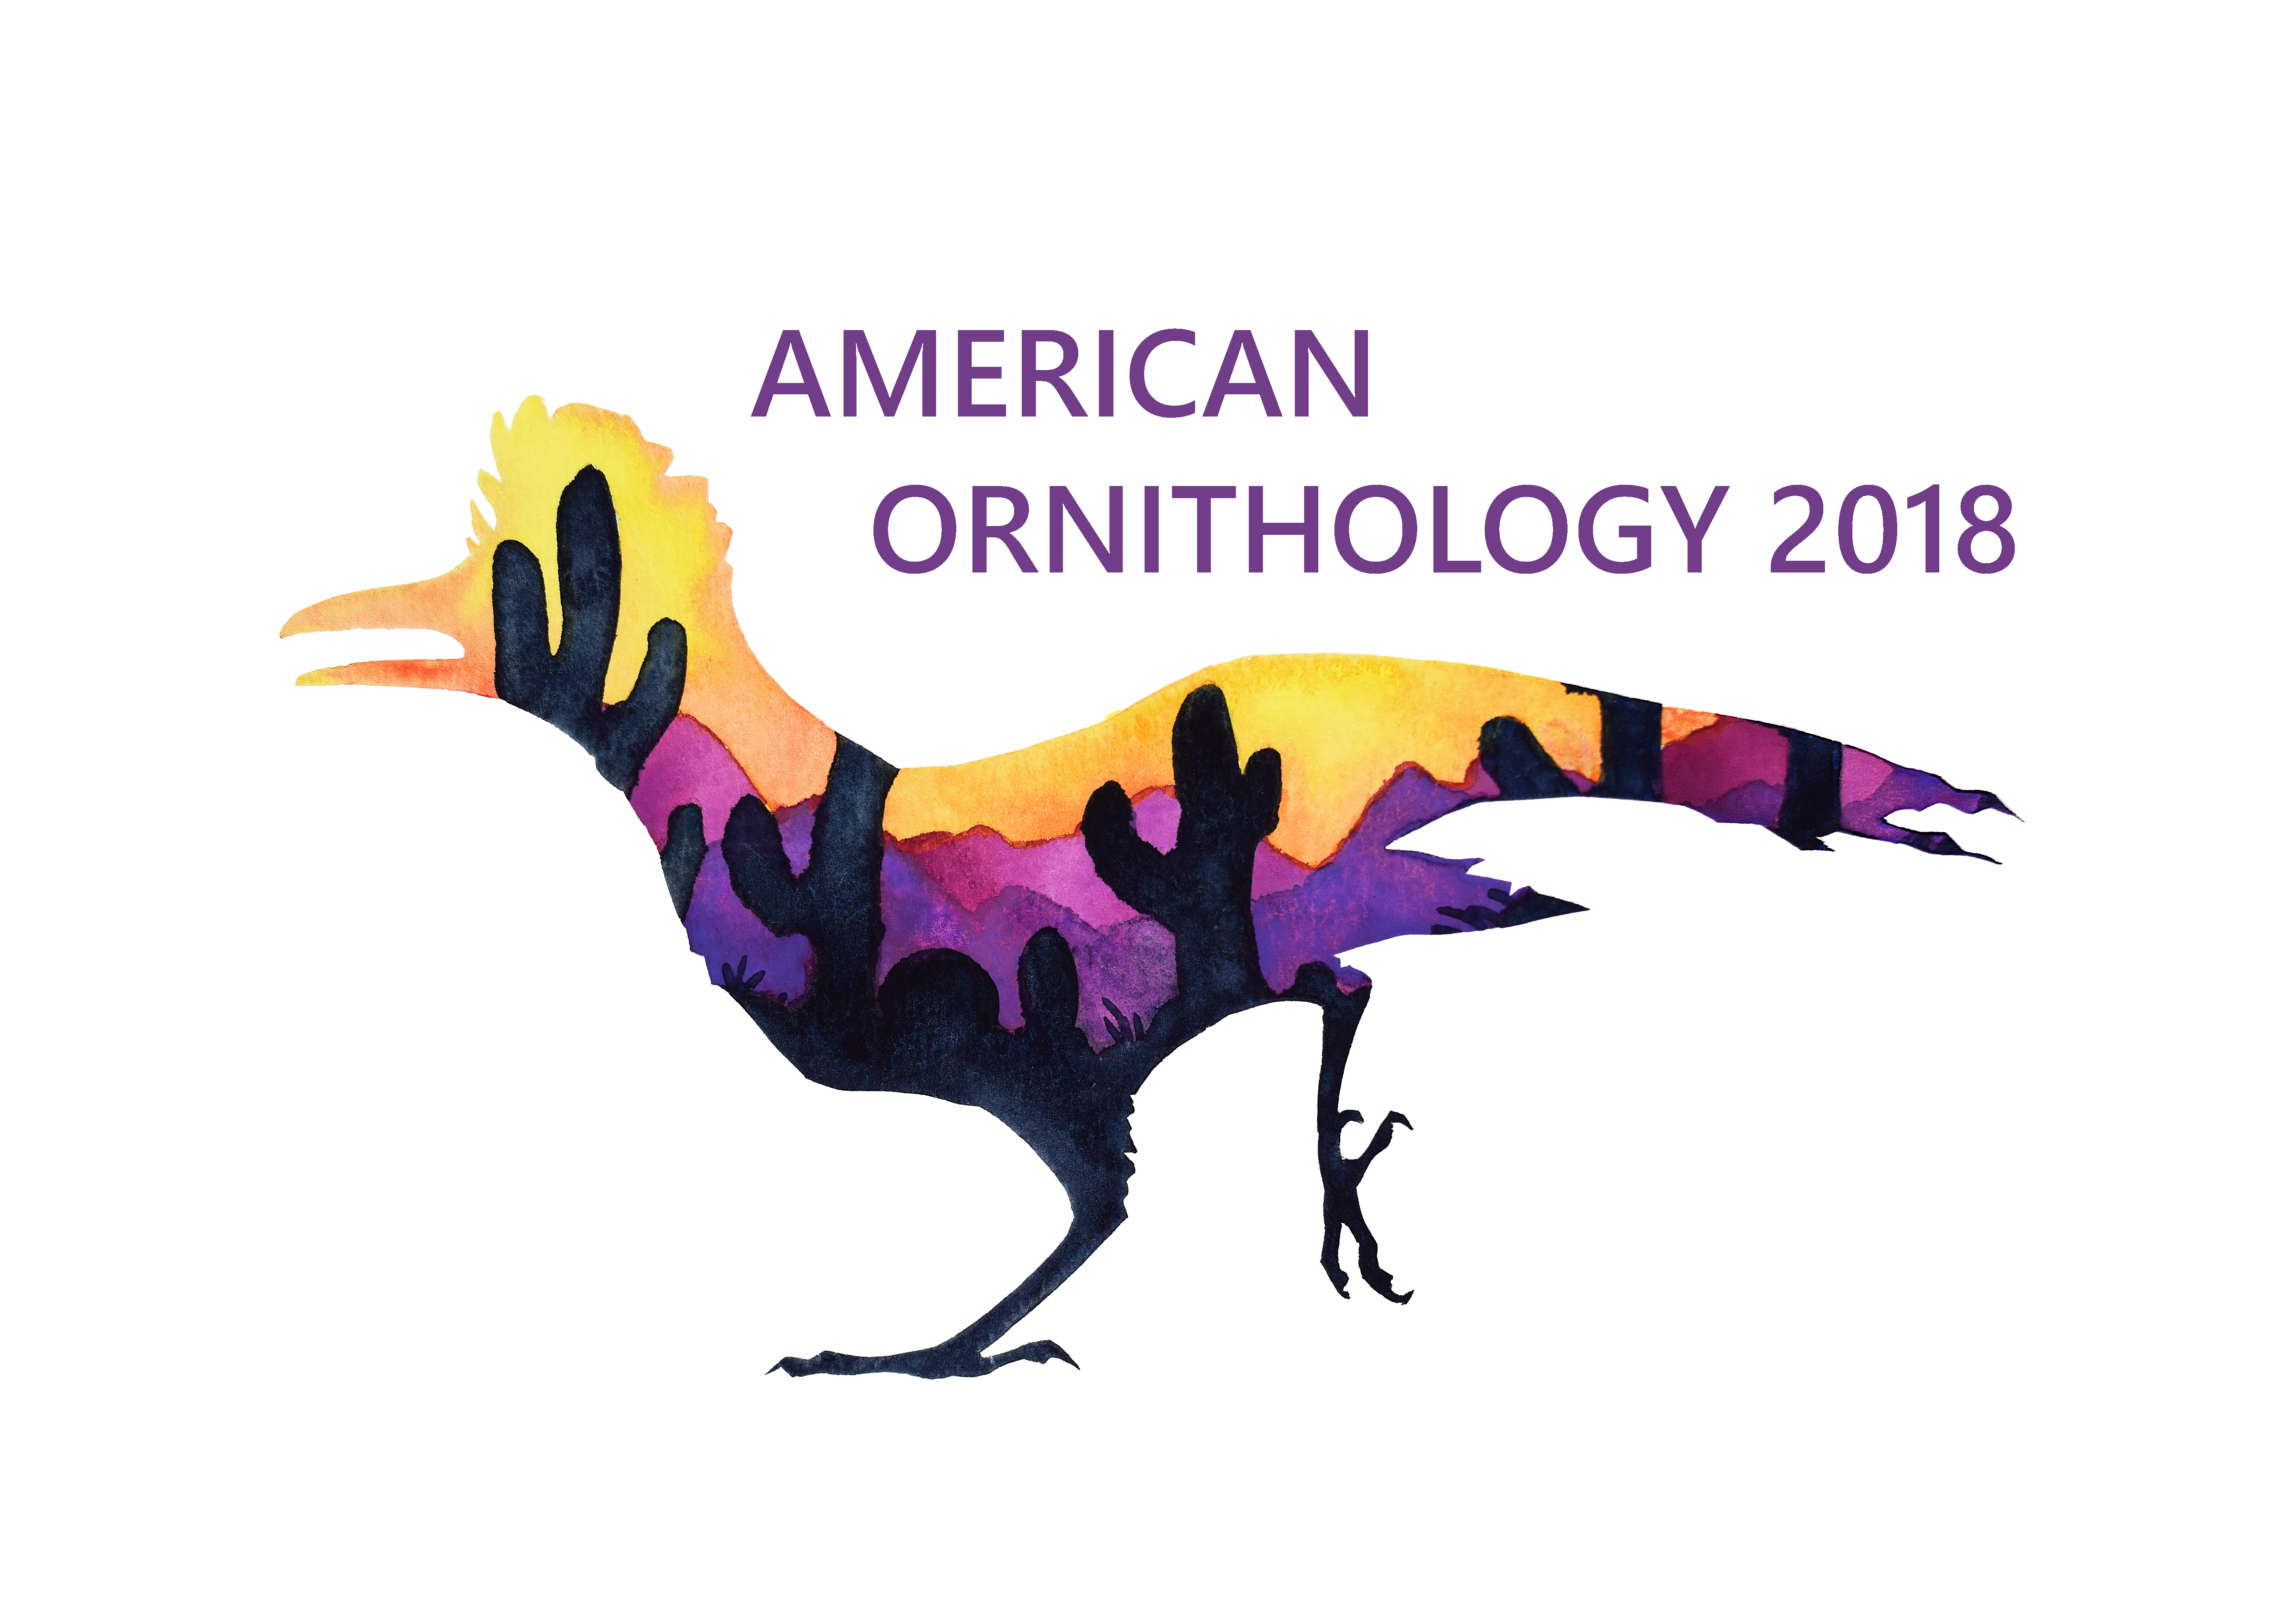
\includegraphics[width=\textwidth]{/Users/NickMason/Desktop/Service/AOS_ProgramBooklet/Tucson2018/AbstractBooklet/AOS2018logo-transparent.png}
    
    \vspace{20pt}
    
    \huge{ABSTRACT BOOK}
   
    \vspace{20pt}
    
    \huge{Listed alphabetically by last name of presenting author}
    
    \tableofcontents

	
\end{center}

\newpage

\begin{center}
\addcontentsline{toc}{subsection}{Oral Presentations}
\Large{\textbf{ORAL PRESENTATIONS}}
\end{center}

\begin{multicols*}{2}
\normaltalk{Combining citizen science with targeted monitoring for Gulf of Mexico tidal marsh birds}{Evan M Adams\\Mark S Woodrey\\Scott A Rush\\Robert J Cooper}{In 2010, the Deepwater Horizon oil spill affected many marsh birds in the Gulf of Mexico; yet, a lack of prior monitoring data made assessing impacts to these the population impacts difficult. As a result, the Gulf of Mexico Avian Monitoring Network (GoMAMN) was established, with one of its objectives being to maximize the value of avian monitoring projects across the region. However, large scale assessments of these species are often limited, tidal marsh habitat in this region is extensive and marsh birds are notoriously difficult to detect on surveys. Citizen science projects could fill in some of these survey limitations and provide better estimates of abundance or distribution but they also could have detectability rates that are too low to be useful. Using observations reported by eBird, we determined how often marsh birds were reported in and around tidal marsh habitats. Clapper Rails were observed in 4.3\% of such surveys; Seaside Sparrows and Least Bitterns were observed in 0.9\% and 2.6\%. Detection rates improved with the type of eBird survey protocol used, survey time, number of observers and proximity to tidal marsh habitat. By selecting citizen science survey effort that has a higher chance of detecting marsh birds, we could be able to achieve reasonable estimates of occupancy with enough survey effort. Integrating citizen science data with data from targeted monitoring projects could then be useful to better describe the distribution of marsh birds in the Gulf of Mexico.}

\normaltalk{Using a structured decision making framework to support large-scale inference}{Evan M Adams\\Auriel M Fournier\\James E Lyons\\Mark S Woodrey}{In the previous talks in this symposium we discuss how a structured decision making (SDM) framework is used to prioritize various kinds of monitoring efforts and craft monitoring plans in the Gulf of Mexico. Here, we argue how the framework allows for effective large-scale inference and integration of multiple monitoring efforts. Scientists and decision-makers are interested in a range of outcomes at the regional scale, including estimates of population size and population trend to answering questions about how management actions or ecological questions influence bird populations. The SDM framework supports these inferences in several ways by: (1) monitoring projects with synergistic activities ranging from using approved standardized protocols, flexible data sharing policies, and leveraging multiple project partners; (2) rigorous data collection that make it possible to integrate multiple monitoring projects; and (3) monitoring efforts that cover multiple priorities such that projects designed for status assessment can also be useful for learning or describing responses to management activities. By prioritizing large-scale inference, we will be able to establish regional baseline population sizes for many bird species and better distinguish reasons for population change and what kinds of management actions are viable recovery options. Previous to this regional focus, we lacked the data and the partnerships to even consider answering questions at the scale of the Gulf of Mexico; by using a structured decision making framework with a focus on regional objectives we are able prioritize such outcomes and support the needs of conservation decision-makers.}

\normaltalk{Genomic data provide a flicker of hope for differentiating taxa in the Northern Flicker complex}{Stepfanie M Aguillon\\Leonardo Campagna\\Richard G Harrison\\Irby J Lovette}{Next-generation sequencing technologies are increasingly being employed to explore patterns of genomic variation in avian taxa previously characterized using morphology and/or traditional genetic markers. The hybridization dynamics of the Northern Flicker complex have received considerable attention, primarily due to the conspicuous plumage differences among these birds and the geographically extensive hybrid zone between the Red-shafted (Colaptes auratus cafer) and Yellow-shafted (Colaptes auratus auratus) flickers in the Great Plains region of North America. However, no traditional molecular techniques have been able to differentiate these two morphologically well-defined taxa from one another, or from the closely related Gilded Flicker (Colaptes chrysoides). Here, we use a next-generation sequencing approach to assess the genetic diversity and evolutionary history of these three taxa. We confirm the overall low levels of differentiation found using traditional molecular markers, but are able to distinguish between the three subgroups for the first time, using a dataset of thousands of SNP loci distributed across the genome. Through demographic modeling and phylogenetic reconstructions, we find that Red-shafted and Yellow-shafted flickers are likely sister taxa, and that their divergence from the Gilded Flicker was comparatively ancient. The low level of divergence and lack of fixed differences between Red-shafted and Yellow-shafted flickers, in particular, suggests whole genome re-sequencing may be necessary to assess the dynamics of their hybridization and identify the genetic basis of their striking differences in plumage.}

\normaltalk{Habitats and Conservation of Molt-migrant Birds in Southeastern Arizona and Northwestern Mexico}{Steven K Albert\\Peter Pyle\\Mary Chambers\\Wade Leitner\\Rodney B Siegel}{Adults of several species of western North American passerines are known to migrate to the monsoon regions of the southwestern U.S. and northwestern Mexico from July to October to undergo molt, and there is growing concern about conservation of habitats needed by these birds during this energetically-demanding time. For two seasons, we documented habitat use by 12 species of monsoonal molt-migrants using mist-netting and area-search. Molt-migrants generally selected habitats similar to those used in their breeding territories; however, in some cases, species appeared to shift habitats for molt in response to environmental effects, including relative strength of the monsoon season. In a separate study, we used archival micro-GPS tags to track the movements of two male Black-headed Grosbeaks (Pheucticus melanocephalus) during their full annual cycle. The seasonal timing of their movements and a prolonged late summer stopover in Sonora, Mexico are consistent with the expected behavior of a molt-migrating bird. Remote-sensed enhanced vegetation index (EVI, a measure of the quantity of live vegetation) data indicated that the grosbeaks arrived in the monsoon region near the area's annual EVI peak, and left as the index was sharply declining. Our results underscore the need to conserve native grasslands and riparian areas -- habitats in which we detected molt-migrants most frequently -- and the need to conserve a mosaic of habitats to account for adaptive selection in response to variable environmental conditions.}

\normaltalk{New initiatives at cooperative bird banding stations aid the conservation of migratory species}{Steven Albert\\James Saracco\\Kristen Ruegg}{The Monitoring Avian Productivity and Survivorship (MAPS) and Monitoring Overwinter Survival (MoSI) Programs comprise the hemisphere's longest-running and geographically most-extensive network of demographic monitoring and bird banding stations, covering nearly 500 active stations in nearly every U.S. state, several Canadian provinces, and 13 countries in Latin America. Many stations are run or aided by citizen scientists. The network was originally established to monitor avian vital rates – especially productivity, survivorship, and recruitment – but new technologies, methods of analysis, and emerging threats have broadened the scope of work carried out at these stations. We will describe three areas of new and emerging research aided by the citizen scientists of the MAPS and MoSI network. (1) Studies of avian disease dynamics: MAPS operators contributed to a study of the ways in which west Nile virus affected survival in 49 species of landbirds. Results indicated that the virus negatively impacted survival in some species only during initial spread of the disease, while others showed no signs of recovery since disease introduction. (2) Studies of migratory connectivity - MAPS and MoSI operators collect feathers from the same species on the breeding, migration, and wintering grounds. Subsequent genetic analysis demonstrates links between discrete populations of breeding and wintering populations and sites, and differences in the timing of migration by different populations. (3) Integrated population models: Models that combine data from MAPS with the North American Breeding Bird Survey improve inferences about causes of population change across many species' ranges.}

\normaltalk{Integrating an eBird portal and an Avian Knowledge Network node for improved citizen science and bird conservation}{John D Alexander\\Ellie E Armstrong}{eBird Northwest, a regional portal of the international eBird program, serves as the primary citizen science application of Avian Knowledge Northwest, a regional node of the Avian Knowledge Network (AKN). Through this regional integration of eBird and Avian Knowledge Network (AKN) we are demonstrating how these data management and science delivery programs add value to and complement each other. eBird Northwest provides content and services to both bird‐watching and natural resource management communities to better develop, promote, facilitate, and improve upon citizen science throughout the Pacific Northwest. eBird Northwest takes advantage of the eBird platform for the entry, management and analysis of simple bird survey data. For more complicated survey data, Avian Knowledge Northwest uses AKN data structures that account for more detail including specific time intervals, distance bins, and site conditions. Avian Knowledge Northwest also offers a platform for the delivery of regionally-relevant and data-rich decision support tools. By integrating the regional nodes of eBird and Avian Knowledge Network, we can take advantage of unique opportunities that add value to both data management programs. We will provide examples of how the integration of eBird Northwest and Avian Knowledge Northwest is facilitating a diverse range of citizen science projects that are being implemented at both local and regional scales. Our approach demonstrates that the integration of eBird Northwest and Avian Knowledge Northwest can improve data collection, data management, and science delivery, and represent an opportunity for enhancing regional bird and habitat conservation programs.}

\normaltalk{Survival, site persistence, and movement dynamics of a non-territorial Neotropical migrant during the nonbreeding period}{Elizabeth M Ames\\Chris Tonra\\Lesley Bulluck}{Understanding survival rates and movement patterns during the nonbreeding period is fundamental to understanding changes in migratory populations as many migrants spend greater than half the annual cycle overwintering. The objective of this study was to estimate survival rates and examine movement patterns of a non-territorial migratory songbird during the overwinter period across a habitat gradient. The Prothonotary Warbler (Protonotaria citrea) is a Neotropical migrant that specializes on forested wetland habitat: bottomland hardwoods during the breeding season and mangrove forest, one of the most endangered forest types globally, during the winter season. In order to estimate survival and track movement patterns we deployed nanotags on individuals across five sites (n=29) located along the Panama Canal. We estimated monthly survival to be 0.966 for after second year birds and 0.967 for second year birds. The best model for predicting survival over the duration of the study contained scaled mass index and time since tagging. The top model describing site persistence included time since tagging and estimated overall site persistence at 0.702. However three other models were closely ranked: time and sex, mangrove habitat and time, and age and time. As the Neotropical dry season progressed, mangrove habitat retained more birds and those birds moved less than those in non-mangrove habitat. Focusing conservation efforts on high quality, wet mangroves would likely provide the best habitat for the greatest number of birds, however conserving secondary forests and wooded wetlands, especially those adjacent to mangroves, may also provide useful habitat.}

\normaltalk{Avian responses to indigenous community forest management in western Amazonia}{Nico Arcilla\\Madison Sutton\\Oscar Tsamajain-Shiwig\\Robert J Cooper}{Tropical forests are singularly critical to maintaining the Earth's biodiversity. Birds play a major part in maintaining tropical forests, where up to 90\% of plant species are dependent on animal pollination and dispersal, and in turn, approximately 30\% of the world's bird species are dependent on tropical forest for survival. Half of the world's remaining tropical forests are in Latin America, especially Amazonia. Indigenous territories comprise about a third of the land area in Amazonia, where they form a major barrier to deforestation, but the effects of indigenous forest management on birds have not been quantified until now. We documented forest management practices in indigenous territories in the northern Peruvian Amazon and investigated their impacts on understory bird communities. We sampled birds in forest stands with different logging histories and used quantitative models to estimate and compare bird community responses. Indigenous logging practices did not result in significant decreases in bird abundance or species richness. However, a third of unlogged forest understory bird species were absent from logged forest between 1 and 5 years post-logging, a loss that was offset by influxes of nearly equal numbers of other avian species that may be better adapted to forest with more open canopy. While indigenous logging practices influenced bird community dynamics, they appeared to be far less detrimental for birds than either conventional or reduced-impact logging. Our results suggest that indigenous territories may approximate sustainable forest and wildlife management to a greater extent than any other logging practices documented in tropical forests.}

\normaltalk{Temperature \& life history: effect of temperature manipulation during incubation on immunity and thermoregulatory performance}{Daniel R Ardia}{Developmental conditions during early life can have effects on physiology in later life history stages. Using temperature modifications during development I have studied how temperature programs organismal performance. Temperature can drive physiological development through simple allocation tradeoffs or can adjust developmental programming, such as through perinatal programming. Experimental heating of developing tree swallow eggs led to transient increases in body condition and body mass in nestlings, whereas experimental cooling led to long-term lower innate immunity measured as bacteria killing ability. Temperature manipulation during embryonic development also affected thermoregulatory ability. Cooled nestlings were less effective at holding body temperature against a thermal challenge. However, cold conditions led to improved performance; by day 12 nestlings in the cooled treatment incur lower thermoregulatory costs, measured by metabolic rate, during a cooling challenge. In captive studies using artificial incubation, both zebra finches and bobwhite quail show effects of temperature manipulation on bacteria killing ability, with embryos cooled during incubation showing reduced performance as nestlings. In quail, individuals experiencing cooler incubation conditions had lower basal metabolic rates, which in turn drove differences in thermoregulatory performance. These results suggest that embryonic development conditions can have developmental effects on immunity, thermoregulatory performance, and metabolic rate.}

\normaltalk{Parrot border crossing?: Biology and conservation of endangered red-crowned parrots in the Rio Grande Valley of Texas}{Caleb M Arellano\\Anthony K Henehan\\Clifford E Shackelford\\Karl S Berg}{Parrots are among the most threatened groups of birds. This is especially true of neotropical parrots, some of which have become established in metropolitan areas of the U.S. Most cases are the likely result of accidental introductions from escaped pets. One interesting exception is the globally endangered Red-crowned Parrot (Amazona viridigenalis), recently established in the Rio Grande Valley of South Texas. Historically considered endemic to northeastern Mexico, the species' original northern range extended close to the U.S. Mexico border, raising questions of the population's origins. . Regardless, the area contains one of the fastest growing human populations in the U.S., leading to destruction of nest sites and illegal pet trafficking., Despite these threats, little is known about population size or breeding requirements. We studied nesting biology and conducted monthly estimates of population size at a communal roost in Brownsville, Texas from Jan 2016 – Dec 2017. Red-crowned Parrots bred almost exclusively in cavities in dead palm trees. Breeding occurred from Mar – Jul in each year and broods contained up to three nestlings. Roosting estimates during the breeding period (ca. 150 individuals) were typically more than half that recorded during the non-breeding period (ca. 250) in both years, suggesting that less than half of the population may have attempted to breed each year. We documented the destruction of a significant portion of nest cavities raising the question of whether artificial nest cavities may mitigate any future shortages.}

\normaltalk{Definition of arid-Zone Carduelini Finches by DNA Phylogeography:American and Asian G. Carpodacus is Taxonomically Split}{Antonio Arnaiz-Villena\\Valentin Ruiz-delValle\\Jose Palacio-Gruber\\Cristina Campos\\Ester Muniz}{A group of bird species included within the Carduelini tribe (genera Rhodopechys, Carpodacus and Leucosticte) belongs to the same radiation according to molecular phylogenetic analyses. Our phylogenetic analyses based on nucleotide sequences of the cytochrome b gene (cyt-b) indicate that some of these species (Rhodopechys mongolica, R. githaginea and Carpodacus nipalensis) do not cluster together with their respective phenetically defined allies. Thus, a new group of birds thrives in both hot and cold arid zones and are phenetically distinct, probably because of their adaptation to different extreme environments but may be considered as a new Genus group.. Both maximum likelihood and Bayesian inference methods support the existence of this new evolutionary basal group among finches which might have originated about 14 MYA. A redefinition of genus Carpodacus is needed: one American, and one different Eurasian evolutionary group at least. Also, a new definition of genus Rhodopechys is found: Rhodopechys obsoleta is a greenfinch ancestor, while R. githaginea and mongolica, along with Carpodacus nipalensis, Leucosticte arctoa, and L. tephrocotis, at least, are the “Arid Zone” group of finches defined in this work. The possibility of existence of more phylogenetic splits within genus Carpodacus is put forward.arnaizantonio@gmail.com}

\normaltalk{The Bobolink Project: Helping Farmers Protect Grassland Birds}{Jonathan L Atwood\\Mark LaBarr\\Allan Strong\\Stephen Swallow\\Anwesha Chakrabarti\\Pam Hunt}{Grassland-nesting birds are disappearing in the northeastern United States. This decline is largely due to mowing of hayfields during the weeks that birds like Bobolinks (Dolichonyx oryzivorus) are actively breeding. To protect these birds we are exploring new strategies for promoting conservation on private farms. New England's working farmers face financial pressures that force them to mow earlier and more frequently. The Bobolink Project collects funds from conservation-minded donors that are used to pay participating farmers to modify their mowing schedules, thereby allowing grassland-nesting birds to successfully complete their breeding cycles. We follow a single price, reverse auction process that encourages farmers to offer their acres at the lowest possible cost, thus integrating conservation into the farm business in a way that is comparable and competitive to traditional farm products. In 2017 a total of 17 farms, totaling 257 ha, were included through donations totaling \$38,000. However, available donations only allowed the Project to accept about 50\% of the farmers who sought to participate, raising a fundamental question about whether annually repeated donor solicitation, aimed at short-term “rental” of fields that in the next year will once again need to be subsidized, is a more successful approach than efforts focused on outright purchase of these properties.}

\normaltalk{Genomic underpinnings of acrobatic social displays in neotropical manakins (Pipridae)}{Christopher N Balakrishnan\\Robert J Driver\\Lainy B Day\\James B Pease\\Matthew J Fuxjager}{Manakins are neotropical suboscines with acrobatic sexual displays performed using the fastest known vertebrate limb muscles. The Scapulohumeralis caudalis (SH) muscle is responsible for medial movement of the humerus and is integral for manakin displays with complex wing movements. Previous studies have revealed elevated androgen receptor (AR) expression in the SH muscle of species with complex wing displays. In this study we used RNA-seq to characterize in detail the regulatory changes associated with the evolution of complex wing displays in manakins. We obtained transcript expression levels derived from the SH and Pectoralis (PEC) muscles from six manakin species and a flycatcher (Tyrannidae). We compared expression levels of 7,194 transcripts between species with and without rapid wing movements, and found differential expression associated with skeletal muscle contraction, muscle filament sliding, and actin-mediated cell contraction gene ontology (GO) categories. Our analyses confirm the up-regulation of AR but also reveal differential expression of AR-associated heat shock proteins and downstream transcription factors. Ongoing analyses will examine rates and patterns of molecular evolution and test for signatures of positive selection on these genes.}

\normaltalk{Response of a native Hawaiian bird to the removal of an invasive predator in a mesic, montane forest}{Paul C Banko\\Kelly A Jaenecke\\Robert W Peck}{Introduced rats are notorious predators of birds and their nests worldwide, but especially on remote islands. Rats (Rattus exulans) first arrived in Hawai‘i with Polynesian colonists about 1,000 years ago, resulting in deleterious consequences for native birds and ecosystems. Since Western contact in 1778, two additional rat species have become established in Hawai‘i, including the highly invasive black rat (R. rattus), which arrived in the late 1800's. Black rats have contributed substantially to the historical loss of native forest bird populations, in part through nest depredation. We assessed the impact of rat depredation on the reproduction of a relatively common native forest bird, Hawai‘i ‘elepaio (HAEL; Chasiempis sandwichensis) by reducing rat populations in two treatment plots in a Before-After-Control-Impact study in mesic montane forest in Hawai‘i Volcanoes National Park. After monitoring rat abundance and HAEL nesting success for two years (2015-16), we distributed diphacinone rodenticide at the beginning of the HAEL nesting season in 2017. Diphacinone bait stations were distributed at 50-m intervals within 700x700m plots at low (1360m) and high (1670m) elevations, which also differed in habitat structure. By the end of the nesting season, rat abundance on treatment plots had been reduced to $<$10\% of levels observed in the previous two years, while it remained relatively unchanged on untreated plots. Analyses indicated that HAEL nest success and daily survival rate (n=206 nests, 3 years) increased on treatment plots during the application of rodenticide. Our results highlight the conservation benefits of removing invasive predators from island ecosystems.}

\normaltalk{The life cycle of Toxoplasma gondii and its impact on wildlife}{Michelle M Barbieri}{Toxoplasma gondii infections are common and widespread among avian and mammalian wildlife from polar to tropical regions. Infections range from asymptomatic to lethal and may vary based on the strain of T. gondii and the immune status of the host. In some threatened and endangered species, they have caused concerning levels of morbidity and mortality. Exposure in wildlife occurs through direct ingestion of oocysts or tissue cysts in prey. Transplacental infections have also been described. T. gondii is a coccidian parasite and its two-stage life cycle is dependent upon felids, the definitive host, for sexual reproduction. This definitive host, which includes outdoor and feral cats, is abundant and each individual can shed millions of oocysts into the environment through feces. A single oocyst is sufficient to transmit infection and oocysts are persistent in the environment, surviving in soil, salt and fresh water for months to years. Oocysts deposited in the terrestrial environment threaten aquatic species via runoff, where they may be taken up by filter feeding fish and invertebrates and transferred to higher trophic levels. Discerning the risk factors for exposure and the development of clinical toxoplasmosis is challenging in wildlife, especially in species that are highly mobile and have diverse foraging habits. The cryptic nature of failed pregnancies, the lack of carcass detection, and the potential sub-lethal impacts of infections further complicate this risk assessment for many populations.}

\normaltalk{Avian communities are decreasing with pi\~{n}on pine mortality in the southwest}{Andrew W Bartlow\\Charles D Hathcock\\Jeanne M Fair}{Tree mortality is expected to increase worldwide due to climate-induced drought and increasing temperatures. The 2000–2002 drought in the southwestern U.S. led to severe outbreaks of bark beetles that resulted in high mortality of ponderosa pine (Pinus ponderosa), Douglas-fir (Pseudotsuga menziesii), and piñon pine (P. edulis) trees. Many areas in piñon-juniper habitat had entire stands of piñon die, especially on the Pajarito Plateau in Northern New Mexico. We compared avian use in areas on Los Alamos National Laboratory (LANL) and Bandelier National Monument property with high pine tree mortality and low tree mortality. LANL sites had also been thinned in 2002, while Bandelier sites were not thinned. We used mist net data and point count surveys to determine avian responses to tree thinning and tree mortality. We continued point counts until 2013. In 2003, avian use of thinned sites did not differ from unthinned sites. Furthermore, tree mortality did not result in fewer species or fewer individual birds, suggesting avian use was not negatively impacted the first year following tree thinning or tree mortality. In 2013, piñon mortality was nearly 100\% at each site. Point counts showed species richness and abundance declined from 2003 to 2013. There was an 83\% decrease in abundance and a 44\% decrease in richness. Abundance declined faster in thinned sites than unthinned sites during this period, but richness decreased similarly in both treatments. Piñon mortality is a threat to bird communities in the southwest, and tree thinning to control fire may be an added risk.}

\normaltalk{Heavy babies and skinny youth: Density dependence in a highly social bird}{Sahas S Barve\\Walter D Koenig\\Eric L Walters}{Increasing population size leads to density-dependent effects that substantially influence species. For group-living, territorial species, density dependence might act at both the group and population levels. We teased apart the relative importance of group- versus population-level density-dependent effects on the body mass of cooperatively breeding acorn woodpeckers (Melanerpes formicivorus) using a 33-year dataset of a dramatically increasing population. Additionally, we examined how density-dependent effects are nuanced by the social status (helper or breeder) of individuals, highlighting its relevance to their sociobiology. On one hand, we show that nestling body mass increases with population density but is unaffected by group size. On the other hand, adult body mass is strongly driven by group-level effects, declining with increasing group size. Density dependence thus works at both group and population levels and leads to opposing outcomes on the size of nestlings and adults. Notably, the body mass of helper males, the philopatric sex, was not only affected by group size but also declined with increasing population density. This result demonstrates a social context driven density-dependent effect previously unknown in cooperatively breeding birds. While multiple hypotheses predict that group size of cooperative breeders should increase with population density, our results reveal strong costs of living in large groups on the body condition of helpers, which likely regulate the decision to remain on the natal territory as helpers or to disperse to become breeders, limiting group size in cooperative breeders.}

\normaltalk{Uncovering the effects of climate change on bird species using structured citizen science: Audubon's Climate Watch program}{Brooke L Bateman\\Nicole Michel\\Kathy Dale\\Zach Slavin\\Chad Wilsey\\Gary Langham}{Species are facing an unprecedented rate of climate change, with over half of North American bird species at risk to lose 50\% or more of their current climatic range by the end of the century. In an uncertain future, we must be able to both forecast and monitor how species are responding to climate change. To track climate effects throughout species' ranges requires a landscape-scale coordinated and a structured effort. Historically, citizen science efforts have been integral in providing bird data through time, however often do not provide structured protocols designed to answer specific research questions. Monitoring change on the landscape in relation to climate change requires a coordinated and more structured effort- monitoring with purpose. Here we will highlight the history of bird citizen science programs, and how we are developing new methods that are better able to detect and forecast change in bird populations in the face of climate change. We will focus on Audubon's newest citizen science effort, Climate Watch, which integrates climate projections and an occupancy modeling framework with community scientists' local knowledge to track how birds are responding to climate change. By monitoring bird responses to climate change as it is happening using a structured monitoring protocol, we can directly test hypotheses about bird climate change responses.}

\normaltalk{Sorting of some basic concepts associated with diversification in birds}{John M Bates}{Diversification is a general term covering processes underlying how groups like birds have evolved. The processes by which different birds have come to occur throughout the world are the subject of new types of data and a range of modern analytical tools allowing both broader and more detailed analyses. I discuss two terms commonly associated with diversification in birds and other organisms, these terms: dispersal and vicariance, are both important, but I argue that there are common issues associated with how these words frequently are used that impede accurate interpretation of diversification throughout the avian tree. I suggest considering these process in a broader biological context is a valuable framework to better understand the forces shaping avian diversification.}

\normaltalk{Low amplitude vocal signaling by rock wrens}{Lauryn Benedict\\Nadje Najar\\Stephanie Pitt}{Birds produce a staggering diversity of sounds. The vast majority of research on this topic focuses on high amplitude broadcast song given by males, but studying other acoustic signal types can reveal much about functional avian communication. Many species produce low amplitude vocalizations that have been variously classified as calls and songs, and generally seem to mediate close-distance encounters between rivals or mates. Rock wrens (Salpinctes obsoletus) frequently use a stereotyped low amplitude signal that differs from both broadcast song and typical contact calls. Measurements indicate that these low amplitude vocalizations have significantly less power than broadcast song (p $<$ 0.0001) and observations indicate that they transmit shorter distances. Rock wrens use the signal most frequently in two contexts: 1) during mate interactions, and 2) when challenged by a conspecific. In the latter context, they often embed the signal within bouts of broadcast song. The varied use of this low-amplitude vocalization implies multifunctionality within close-range encounters. Like song, it appears to function both in mate communication and resource defense, but allows individuals an alternative signaling option within these contexts.}

\normaltalk{Higher spring temperatures increase food scarcity and limit the distribution of crossbills}{Craig W Benkman\\Eduardo T Mezquida\\Jens-Christian Svenning\\Ron W Summers}{Understanding how climate affects species distributions remains a major challenge, with the relative importance of direct physiological effects versus biotic interactions still poorly understood. Here, we focus on three species of crossbill (Loxia spp.) in Europe. Although crossbills will feed on seeds in the cones of Scots pine (Pinus sylvestris) throughout its wide range in Europe, crossbills specialize on Scots pine in only northern Europe and Scotland, where parrot (L. pytyopsittacus) and Scottish crossbills (L. scotica) reside, respectively. The widespread common crossbill (L. curvirostra) feeds primarily on seeds in the cones of spruce (Picea) in northern Europe and various species of pine in southern Europe. We test the hypothesis that warmer temperatures in the spring accelerate seed release from Scots pine cones, thereby lengthening the period of food scarcity before the following seed crop is available in summer, and thus preventing year-round specialization on Scots pine seeds outside of northern Europe and Scotland. We found that seed fall occurred 1.5–2 months earlier in southern Europe (Spain) than in Sweden and Scotland, and was associated with variation in spring maximum temperatures and precipitation. These climate variables and area covered with conifers relied on by the crossbills explained much of their observed distributions, consistent with an indirect influence of climate through its effect on food plants and seed availability. Using these relationships to project future distributions (2070) under global change scenarios revealed reductions in potential crossbill distributions, especially for Parrot Crossbills.}

\normaltalk{Can citizen scientists provide reliable avian count data in low diversity neotropical areas?}{Nicholas P Bergen\\Nicola Koper}{Monitoring projects in neotropical areas often lack the necessary resources and professional personnel to conduct consistent, large scale monitoring. Few studies have considered using non-expert observers to collect avian abundance data. However, citizen scientists have the potential to contribute meaningful data to this knowledge gap in low diversity areas. In this study, citizen scientists in Grenada carried out dependent double observer surveys of resident land birds. 34 volunteers were trained in audio and visual species identification and standardized survey methods. We used models in the program DOBSERV to test for species-specific, observer-specific and group-specific differences in detectability. We also tested the effects of observer ability on observed abundance and species richness. Expert observers had significantly higher observed abundance compared to novice observers for difficult to detect species, but we found no evidence of different observed abundance for most common species. We found evidence of observer effects on detectability for 19 of 23 field trials. While individual observer detection probabilities increased with ability, the probability that at least one observer detected an individual was high ($>$90\%) for 20 of 23 trials. This suggests that in areas with low diversity, pairs of well trained observers with little previous experience can collect reliable abundance data, especially for common species, and that dependent double observer methods would increase the accuracy of abundance estimates for non-expert observers.}

\normaltalk{Twenty-five Year Impact of the Northwest Forest Plan on Forest Composition and Bird Populations}{Matthew G Betts\\Benjamin T Phalan\\Joseph M Northrup\\Zhiqiang Yang\\Robert Deal\\Jos\'{e}e Rousseau}{The 1994 implementation of the Northwest Forest Plan in Oregon, Washington and California resulted in one of the most rapid and broad-scale changes to forest management in the world, ultimately affecting practices on 24.5 million acres. This provides an unprecedented opportunity to evaluate the degree to which policy has influenced biodiversity over the long term, a critical component of adaptive management. We relied on the 25 years of region-wide bird surveys, annual remotely sensed forest cover data, and landownership information to test hypotheses about the response by forest birds to the NWFP. Bayesian hierarchical models revealed that population trends of both early and late seral species were predicted well by changes in forest composition. However, counter to our expectations, mature-forest associated birds declined more rapidly following the NWFP than prior to its establishment. We hypothesize that temporal lags in bird responses to prior habitat loss, climate changes, and negative responses to contemporary thinning may explain these declines. Early seral species continue to decline on both federal and private lands, likely due to a combination of intensification of forest management practices on private and succession on federal lands. Overall, these findings indicate that although the NWFP has substantially slowed declines in old growth forest, this change has yet to have a positive impact on late-seral bird populations. This may also call into question the urgency to promote early seral habitat at the expense of the conservation and restoration of old forest on federal lands, at least for these bird species.}

\normaltalk{Conservation of Sick's Swifts (Chaetura meridionalis) in Southern Brazil: a successful citizen science initiative}{Renata N Biancalana}{The breeding habits of swifts from the genus Chaetura that live in urban environments are often associated with human made structures, such as chimneys. This behavior, in many cases, approximate people and birds, since they become part of each others everyday life for a certain period of time. In southeastern Brazil Sick's Swift is a common urban species that frequently uses chimneys to place their nests. Accidents with falling nests and nestlings are common, and mortality in rehabilitation centers is high due to a lack of information and protocols to recover swift nestlings. In the state of São Paulo, during two consecutive years a successful citizen science initiative has taken place to try to rehabilitate Sick's Swifts nestlings. From November to December 2016 three nestlings were found together with their nest in the bottom of a barbecue grill from a house. They had different stages of plumage. Two nestlings died and one successfully fledged. In November 2017 three nestlings were found in the same place and four nestlings from a neighboring city were brought to a swift rehabilitator. Again, both clutches had nestlings with different plumage development stages. From the seven rescued nestlings, five fledged between the beginning and the end of December 2017. Several aspects of the nestlings behavior that have never been reported before were observed. This is the first case of a initiative to rehabilitate swifts in Brazil and with more investment in education and training, further rescue projects can be implemented in the country.}

\normaltalk{Introgression across the Great Plains towhee hybrid zone characterized with historical DNA}{Shawn M Billerman\\Bronwyn G Butcher\\Irby J Lovette}{Hybrid zones—locations where two previously isolated populations come into secondary contact and interbreed—are often regarded as natural laboratories that can provide powerful insights into the differences that contribute most importantly to reproductive isolation between taxa. In part owing to their past prominence in classical studies of hybridization dynamics, the avian hybrid zones of the Great Plains represent a particularly powerful system in which to explore mechanisms important for the maintenance of biodiversity on a large geographic scale. While there is an extensive and valuable history of research on most of these hybrid zones, the hybrid zone between Eastern (Pipilo erythrophthalmus) and Spotted towhees (P. maculatus) has not been studied since the 1950s. We take advantage of a valuable series of specimens collected over 60 years ago, combined with new genomics tools, to investigate patterns of genetic and phenotypic introgression between towhees across the Great Plains. This first in-depth analysis of genetic introgression between Eastern and Spotted towhees will help us to understand hybridization and speciation in the context of other well-studied systems across the Great Plains. Analyses of phenotypes from the towhee hybrid zone suggest extensive introgression, with high proportions of intermediate phenotypes relative to parentals, differing from other hybrid zones of the Great Plains, where intermediate phenotypes represent a relatively small proportion of individuals. These differences suggest different selection pressures between these systems, and may help us better understand how and why these hybrid zones are maintained across the Great Plains.}

\normaltalk{Testosterone in a sex-role reversed and polyandrous bird: Female aggression, ornamentation, and reproductive success}{Misha A Blizard}{Despite abundant evidence of testosterone’s function in male behavior and ornamentation, its role in females is less clear. I studied testosterone in an avian species (spotted sandpipers; Actitis macularius) exhibiting sex-role reversal: females experience greater competition for mates than males, are aggressively territorial, and can have multiple mates in one season. I predicted that female plasma testosterone levels would remain high throughout the breeding season, as territory defense and sequential courtship of males continues, while male testosterone levels would drop when caring for offspring. I also expected that testosterone, particularly in females, would correlate with reproductive success and degree of melanized plumage ornamentation. Females maintained constant testosterone levels from courtship to egg laying and early incubation, with significantly lower levels than males during courtship. After courtship, male testosterone dropped to levels comparable to females, supporting previous research on sex-role reversed species. Considering behavior, females captured following a simulated territorial intrusion had higher testosterone levels than females not exposed to a simulated intrusion. Variation in both female and male ornamentation could be explained by models incorporating testosterone levels relative to reproductive stage. However, testosterone did not correlate with the reproductive success of females or males. The maintenance of female testosterone levels throughout the breeding season and the elevation in female testosterone levels following simulated territorial intrusions suggest that testosterone mediates female aggression in spotted sandpipers. The relationship between testosterone and ornamentation in both sexes further strengthens prior findings that this female-biased plumage ornament honestly signals competitive ability.}

\normaltalk{Manipulating badges of status only fools strangers}{Theadora A Block\\Alexis S Chaine\\Daizaburo Shizuka\\Theadora A Block\\Lynn Zhang\\Bruce E Lyon}{Conflict in nature is common and risky, and mechanisms like individual recognition or badges of status can reduce such costs. Badges of status and individual recognition are thought unlikely to coexist in the same population since badges are primarily useful in larger, fluid social groups whereas individual recognition requires smaller, stable groups. Social networks of winter flocks of golden-crowned sparrows (Zonotrichia atricapilla) exhibit intermediate levels of social community structure. We found that dominance mechanism depends on social context. Experiments showed that strangers use badges of status to determine dominance. Conversely, badge experiments with familiar flockmates had no effect on dominance, and these experiments showed decreased aggression relative to experiments with strangers. Our results provide among the first experimental evidence for coexistence of status signals and individual recognition, suggesting that variation in social context, and hence the feasibility of recognition, may help maintain coexistence of these two dominance resolution mechanisms.}

\normaltalk{Variation in male solo song dialects of White-eared Ground-Sparrows (Melozone leucotis; Passerellidae) through time}{Katherine Bonilla\\Luis Sandoval}{For most tropical bird species that learn songs is unknown where or when learning occurs, but, to know this is critical to understand the occurrence or not of song dialects. Three possible hypotheses may explain the dialect occurrence in species that learn songs: (1) Males learn songs from birds in the area where born and stay close when adult, this produces similar songs among individuals in the area. (2) Males learn songs from birds in the area where born but migrate to new areas as an adult, producing a mix of songs in the area where establish the territory. (3) Males learn songs after establishing a territory, producing similar songs among individuals in the area. Our goal was to analyze the dialects change through time on White-eared Ground-Sparrows (Melozone leucotis; Passerellidae) males, as a proxy to understand when or where these males learn to sing, and therefore how dialects are produced in this species. We sound recorded four White-eared Ground-Sparrow populations during seven years (each male was color banded) in Valle Central, Costa Rica. During the study period, we recorded the number arriving and departing males in each population. We found that song dialects have a small variation through time, although individuals in each population changed. Our data are consistent with hypotheses one and three, but without a genetic study is impossible to discriminate between both. However, we are sure that White-eared Ground-Sparrow males learned songs from conspecifics at the population when they establish the breeding territory.}

\normaltalk{Rapid evolution of plumage traits in African white-eyes: a genomic perspective}{Rauri CK Bowie\\Guinevere O Wogan\\Ke Bi\\Graeme Oatley\\Gary Voelker}{White-eyes (Zosterops) have earned the moniker the “great speciators” by exhibiting among the highest rates of diversification estimated for vertebrates. The rapid speciation among the birds of this group, and the extremely wide geographic distribution (Old World tropics) makes them an interesting group within which to investigate the processes underpinning speciation and adaptation. Here we make use of several thousand genome-wide SNPs to investigate phylogenetic and phylogeographic divergence among African white-eye taxa. We demonstrate that plumage traits have evolved rapidly, with several examples of parallelism reflecting adaptation to local habitats. Finally, by quantification of plumage in modern and historical specimens, we demonstrate that the belly and flank plumage of southern African white-eyes have continued to be selected upon over the past 100 years.}

\normaltalk{Picky eaters: An undergraduate laboratory exercise}{Melissa S Bowlin}{Here, I present a four-hour laboratory exercise suitable for either an ornithology or a comparative animal physiology course. In it, students use calorimetry to measure the energy contained in several different food items. They then observe House Sparrows (Passer domesticus) selecting food items to determine whether or not birds preferentially select the most energy-dense food items. Depending on how it is presented, this lab can teach students about optimal foraging, feeding energetics, essential nutrients (i.e., that birds eat for reasons other than obtaining energy), individual variation in feeding strategies, and basic statistics (importance of multiple samples, Chi-square and ANOVA). I will discuss solutions to problems I have encountered while performing this lab in the past as well as the permissions necessary to perform the experiment.}

\normaltalk{The roles of interspecific aggression and thermal physiology in limiting elevational ranges of tropical birds}{Andy J Boyce\\Blair O Wolf\\Thomas E Martin}{Climate and competition are both strong forces that set range limits and have both been posited as drivers of narrow elevational ranges typical of tropical birds. Narrow elevational ranges result in rapid species turnover across elevations and produce massive biodiversity on tropical mountains, yet our understanding of the forces that produce this pattern are still evolving. To assess the relative importance of climate and competition in setting elevational range limits of tropical birds, we measured thermal physiology and interspecific aggression across a large elevational gradient in Malaysian Borneo. We estimated multiple metrics of thermal physiology (RMR, conductance, LCT) for 28 songbird species from mid (1500m) and high (3200m) elevation communities. Furthermore, we performed playback experiments on two parapatric species pairs and one sympatric species pair. Thermal physiology was similar between mid and high elevation species and there were no consistent differences between parapatric species pairs. We found interspecific aggression in one parapatric pair (Pycnonotidae) and a complete absence of aggression in another (Zosteropidae). We also found interspecific aggression between two species of sympatric flycatchers (Muscicapidae). Our results suggest thermal physiology is not a direct driver of elevational range limits in tropical songbirds. Additionally, interspecific aggression may set range limits in some cases, but the absence of aggression in one parapatric pair and the presence of aggression between co-occuring species indicates aggression is not a prerequisite for parapatry and aggression alone is not evidence that competition sets range limits.}

\normaltalk{Breeding season carry-over effects of forest fragmentation on Wood Thrush (Hylocichla mustelina)}{Brendan Boyd\\Sue Hayes\\Bridget Stutchbury}{The Wood Thrush is an iconic forest-dwelling North American long-distance migrant that has been steadily declining for decades. Habitat loss and fragmentation on the breeding grounds has been shown to cause short-term negative effects on immediate breeding success. However, long-term impacts on adults, or carry-over effects, have not been studied, in part due to the difficulty of tracking individuals across large geographic distances. The Motus Wildlife Tracking System is an innovative new automated radio telemetry array that, for the first time, can link breeding fragment size to fall migration and annual survival. Wood Thrush occupying small fragments are expected to experience high rates of brood parasitism and nest predation, which could directly delay fall migration due to timing constraints from late re-nesting or indirectly delay migration if adults are in poorer condition. Wood Thrush are large enough to carry radio-tags with a one year battery life, allowing detection of adults who return within the 100,000 km2 study site in SW Ontario. I captured adult Wood Thrush (n=47) in large and small forest fragments in SW Ontario during the 2016 and 2017 breeding seasons and fitted them with coded radio transmitters in order to track their movements using the Motus Wildlife Tracking System. I will present results to test two predictions (1) the initiation of fall migration will occur later for birds breeding in small versus large fragments and (2) there will be a lower annual return rate for birds breeding in small versus large fragments.}

\normaltalk{Movement ecology of grassland sparrows and why it matters for conservation}{Alice Boyle}{Understanding the causes of individual-, population-, and species-level differences in dispersal and migration remains a central challenge in ornithology because movements are inherently hard to study but have major implications for their population dynamics. Grassland birds appear to be among the most mobile groups of terrestrial birds. Here I summarize results of studies of Ammodramus sparrows from the tallgrass prairies of Eastern Kansas based on marked individuals, landscape-level attributes, and tracking. Both Grasshopper and Henslow's sparrows exhibit high rates of within-season and between-year breeding dispersal, and in Grasshopper Sparrows, both dispersal propensity and the resulting pay-offs are affected by predation but not brood parasitism risk. Henslow's Sparrows move to larger, less fragmented tracts of grassland as the season progresses. Occupancy, isotopic, and re-sighting data all suggest that (frequently long distance) dispersal between years is the norm in both species. Between-year dispersal occurs in conjunction with migration; thus, I provide preliminary evidence for the non-breeding ranges of Kansas-breeding Grasshopper Sparrows and discuss associations between migration, dispersal, and demographic parameters. Some implications of these studies are bad news for conservation; despite their small size, these birds do best in very large grasslands, they apparently respond to environmental conditions over large scales, and standard approaches do a poor job at revealing links between management and population processes in such dynamic systems. Conversely, the birds' mobility makes them responsive to changing management and local environmental conditions, minimizing the role of dispersal limitation.}

\normaltalk{Problematic Pachycephalidae: a new phylogenetic hypothesis using ultraconserved elements}{Serina S Brady\\Leo Joesph\\Robert G Moyle\\Michael J Andersen}{The utility of islands as natural laboratories of evolution is exemplified in the patterns of differentiation in widespread, phenotypically variable lineages. Pachycephalidae is one of the most complex avian radiations spanning the vast archipelagos of the Indo-Pacific, making it an ideal group to study the patterns and processes of diversification on islands. Here, we present a robust phylogenetic hypothesis for all five genera within Pachycephalidae, based on thousands of ultraconserved elements (UCEs) that we generated with a target-capture approach and high-throughput sequencing. Our dataset comprises 104 individuals and includes 50 species in the family. We sampled more densely within taxonomically recalcitrant clades, such as the Pachycephala pectoralis complex. We estimated a species tree for all whistlers within a multispecies coalescent framework and explored questions pertaining to the groups' systematics and biogeographical origins at multiple taxonomic levels within this clade (e.g., from the entire family to within species-complexes). This work further refines our understanding of one of the regions' most enigmatic bird lineages and adds to our growing knowledge about the patterns and processes of diversification on island systems.}

\normaltalk{Extraordinary genetic similarity between Rufous and Allen's hummingbirds inferred from whole genome sequences}{Alan Brelsford\\German Lagunas-Robles\\Brian Myers\\Kevin Burns\\Chris Clark}{Rufous and Allen's hummingbird males differ in several traits that are likely to be under sexual selection, including coloration, the shape of tail feathers involved in sound production, and courtship display behavior. The recent discovery of a hybrid zone in southern Oregon and northern California raises the possibility of determining the genetic basis of these traits by admixture mapping. In order to determine the extent of genetic differentiation between the species and how differentiation varies among genomic regions, we sequenced the genomes of 7 Allen's and 9 Rufous hummingbirds collected far from the hybrid zone. Out of 1.6 million SNP markers identified, only 81 were fixed for alternative alleles in the two species. These fixed differences were overwhelmingly (82\%) located on the Z chromosome, further supporting the important role of sex chromosomes in speciation. Most of the fixed differences fall outside protein-coding regions, and none cause amino acid substitutions, suggesting that the functional differences between the species are regulatory, not structural. Because fixed differences are limited to a few small regions of the genome, prospects are good for identifying their associations with behavioral and morphological traits by admixture mapping.}

\normaltalk{Urban and Endangered: the complex realities of Red-crowned Parrots in Texas}{Donald J Brightsmith\\Simon Kiacz\\Janice D Boyd}{The US Endangered Species Act was created to protect species and the habitats on which they depend, but like much legislation it sometimes has unexpected impacts. In 2011, the USFWS declared the Red-crowned Parrot (Amazona viridigenalis) as a candidate for listing. This parrot is endemic to northeastern Mexico and is listed as endangered by the IUCN. In the Lower Rio Grande Valley of Texas (LRGV), the species began to appear in the wild in the early 1980's and the population has grown steadily since 1995. Despite ongoing debate, the USFWS and State of Texas consider the population native. Since 2016, we have studied nest trees (98) and roosts (181 counts) throughout the LRGV. Over 70\% of nest trees were standing dead palms of introduced species. Typical roost and nest locations were within 5 meters of residential streets, often in the front yards of private houses. In fact, all roosts and nest sites were in planted trees in suburban areas. Despite the presence of sizeable protected areas, no roosts or nests were discovered in patches of natural vegetation. Nationwide other endangered species exist in suburban environments, but their persistence is normally tied to remnant native vegetation. However, if the Red-crowned Parrot is listed on the US Endangered Species Act, it will present a unique set of challenges for homeowners, governments, and urban ecologists as they struggle with how to maintain critical habitat elements of anthropogenic origin in wholly manmade habitats.}

\normaltalk{Indirect effects of a competitor on life history and reproductive traits in a cavity nesting bird}{Sarah E Britton\\Barbara Ballentine}{Research on life history evolution in birds has revealed both direct and indirect effects of predation. Increased levels of nest predation favor reproductive behaviors that reduce the threat of predators on offspring or allow parents to bet hedge for future reproductive attempts. In this study, we investigate whether the presence of a competitor, the house wren (Troglodytes aedon), results in similar indirect effects on life history and reproductive behaviors of Carolina chickadees (Poecile carolinensis). House wrens compete for nesting cavities and will kill Carolina chickadee eggs and nestlings. We monitored nest boxes in Western North Carolina where exposure to house wrens varies. We surveyed house wren presence at active Carolina chickadee nests and measured clutch size and mass, incubation, provisioning rates, nestling growth rates, development, and fledging success of chickadees. House wren takeover accounted for 38.77\% of nesting failures, more than any other cause of failure in our study. We found that the presence of house wrens resulted in smaller Carolina chickadee clutch sizes. However, we did not detect any effects of house wren presence on chickadee egg size, incubation, provisioning, growth, or development. These results suggest that house wren presence affects a narrow range of life history traits early in the nesting period, possibly because this is when house wrens are the biggest threat. Reducing clutch size may be a strategy used by Carolina chickadees to decrease reproductive investment in an environment where early nest failure is probable, allowing adults to reserve energy for future reproduction.}

\normaltalk{Using Structured Decision Making to Balance Stakeholder Objectives for Red-cockaded Woodpecker Management}{Emily J Brown\\Paige F Ferguson}{The Red-cockaded Woodpecker (Picoides borealis; RCW) is listed as Endangered under the United States Endangered Species Act. The Oakmulgee Ranger District of the Talladega National Forest harbors the largest RCW population in Alabama. Despite efforts to restore RCW habitat and install artificial cavities in the Oakmulgee, the number of active RCW clusters has not exceeded 120, although the District's Recovery Plan objective is 394 active clusters. Our objectives are to identify factors limiting RCW population growth and identify management methods that could reduce these limitations. We held four structured decision making workshops with representatives from the United States Forest Service, the Animal and Plant Health Inspection Service, the Longleaf Alliance, the Birmingham Audubon Society, and local residents. We built a decision network that predicted the relative likelihood of a range of management options to meet stakeholder objectives, including increase the number of RCW clusters. In addition, we collected field data related to factors the decision network identified as influencing the number of RCW clusters. Cavity insert installation had the greatest probability of increasing the number of RCW clusters and prescribed burning was most likely to meet the combination of stakeholder objectives. There was some support for midstory removal meeting stakeholder objectives. Sensitivity analysis of the decision network suggested that the number of RCW clusters is affected by helper and breeder survival, recruitment rates, food availability, and herbaceous understory. The decision network based on stakeholder objectives will be the framework for addressing future questions.}

\normaltalk{Hybridization and introgression after the 19th century invasion of Glossy Ibis (Plegadis falcinellus) into the New World}{Robb T Brumfield\\Jessica A Oswald\\Michael G Harvey\\Rosalind C Remsen\\DePaul U Foxworth\\Donna L Dittmann}{The Glossy Ibis (Plegadis falcinellus) of the Old World colonized the East Coast of the United States in the early 19th Century, and subsequently expanded and came into contact with the indigenous New World White-faced Ibis (P. chihi). Putative hybrids between the two species have been observed across a large portion of North America. To characterize the extent of hybridization and introgression we sequenced 4,616 ultraconserved loci (UCEs) from 66 individuals sampled across the distributions of falcinellus, chihi, and the range-restricted Puna Ibis (P. ridgwayi) of South America, including samples from a contact zone between falcinellus and chihi in southwestern Louisiana. We found differentiation across the genome among the three currently recognized species. Our results also revealed extensive genetic admixture between chihi and falcinellus in birds with both intermediate and parental phenotypes where species are sympatric and also in some individuals sampled far from the contact core area of sympatry. Genomic cline analyses revealed evidence of greater introgression into falcinellus from chihi than vice versa, but did not detect cline width outlier loci that would suggest selection against hybrids. Surprisingly, we also found evidence of admixture between ridgwayi and nearby South American populations of chihi. We expect further population expansion in Plegadis, perhaps driven by anthropogenic environmental changes, to contribute to additional dynamic secondary contact and more introgression among species in the future.}

\normaltalk{Evaluating the relationships between eastern hemlock decline and Louisiana waterthrush demographics and behavior in Tennessee}{Lee C Bryant\\Tiffany A Beachy\\Than J Boves}{Eastern Hemlock (Tsuga canadensis) is declining throughout the eastern United States due to the invasive Hemlock Woolly Adelgid (Adelges tsugae). In the southern Appalachians, hemlock is concentrated in moist ravines and its loss may threaten riparian habitat quality. With respect to birds, most research has examined changes in community diversity but few studies have evaluated the consequences for, and responses by, single species to hemlock decline. The Louisiana Waterthrush (Parkesia motacilla) is an obligate riparian species that could be sensitive to hemlock condition in the southern Appalachians. Environmental changes including habitat fragmentation and stream acidification negatively impact waterthrushes, but how hemlock decline might impact them is currently unclear. To address this issue, we evaluated how hemlock condition was associated with a suite of metrics related to waterthrush behavior or fitness. We found that hemlock condition was unrelated to territory size, provisioning, nestling condition, foraging habitat selection, or adult survival. However, with respect to nest site selection, waterthrushes selected for areas with more exposed roots when hemlock condition was poor. Nest survival was reduced in areas where hardwood species dominated the understory, suggesting that hemlock decline could indirectly impact waterthrush fitness dependent on how succession proceeds following hemlock mortality. In total, our results suggest that short-term consequences of hemlock decline for this charismatic riparian species in Great Smoky Mountains National Park appear minimal but are likely dynamic and complex. Adult waterthrushes may be able to adjust their foraging behavior following hemlock decline, but subsequent habitats could have negative consequences for reproduction.}

\normaltalk{Winter diet composition of Montezuma quail in southern Arizona}{Oscar E Lopez Bujanda\\Alberto Macias Duarte\\Reyna A Castillo Gamez\\Angel B Montoya}{Montezuma quail (Cyrtonyx montezumae) is a popular game bird that inhabits semiarid oak grasslands in southern Arizona, New Mexico, Texas and Mexico. Montezuma quail's diet has been poorly investigated in their northern edge of its distribution. In this regard, investigating the diet composition of Montezuma quail, as well as its temporal and geographic variation, is a fundamental tool for understanding the species' ecology and provides relevant tools for harvest and habitat management. The objective of this research is to determine the composition of the winter diet of C. montezumae in Arizona from quail harvested during the hunting seasons of 2016-2017. We found that acorns of Quercus spp. (46\%) are the most frequent food item in the crops of C. montezumae, followed by grass seeds (19\%), rhizomes of sedge Cyperus fendlerianus (11\%), bulbs of woodsorrel Oxalis spp. (7\%), insects (5\%), seeds of wildbeans Phaseolus (4\%), bulbs of sedge Cyperus spp (2\%) and the rest of the diet (6\%) is represented by 37 plant species and one desert snail (Gastropoda). This result differs from the only two previous studies in Arizona, where the principal food item in winter were the bulbs of Oxalis (up to 65\% of their diet) and the large presence of acorn was only in the spring (41.8\%). This variation in the diet composition suggest a plasticity in resource utilization in response to yearly variation in humidity and temperature.}

\normaltalk{Habitat specific abundance and occupancy dynamics of a non-territorial overwintering songbird in Panama and Colombia}{Lesley P Bulluck\\Nick Bayly\\Elizabeth Ames\\Cathy Viverette\\Chris Tonra}{Despite numerous studies of territorial overwintering migratory songbirds, little is known about the nonbreeding ecology of most migratory species. Non-territorial species present an additional paradigm, as they display more complex movement patterns than territorial species. Recent studies of migratory connectivity in non-territorial Prothonotary Warbler (PROW) indicate that individuals from across disparate breeding populations overwinter in a relatively small region, but little is known about how abundance and occupancy varies among habitats. We surveyed for PROW across $>$300 points in 15 sites throughout this region and used these data to estimate habitat-specific abundance. We found that PROW abundance increases with canopy height in cienaga (lagoon) and mangrove habitats from {raise.17exhbox{\$scriptstylemathtt{sim}\$}}1 bird/ha, when canopy height is 5m, to 3-4 birds/ha when canopy height is 20m. PROW abundance was low ($<$1 bird/ha) in secondary forests and woody wetlands, regardless of canopy height. Survey points were visited twice to develop dynamic occupancy models and assess movement into and out of habitats as the dry season progresses. The probability of PROW site occupancy increased with increasing canopy cover, and mangroves and cienagas are less likely to experience local extinction as the dry season progresses compared with wooded wetlands. Consistent use of sites into the dry season suggests vital resources are present during the pre-migratory period. This study enhances our understanding of Prothonotary Warbler non-breeding habitat use and movement and is one of the first to demonstrate that habitat quality may be correlated with the probability of local extinction in a non-territorial overwintering migrant songbird.}

\normaltalk{Extrapair parentage in a rapidly moving chickadee hybrid zone: confounding factor for analysis of fitness consequences of interbreeding?}{Emily S Burton\\Robert L Curry}{In songbirds that hybridize, extrapair parentage may confound analysis of key fitness consequences such as hatching success if the species-level genotypes of extrapair parents differ from those of social parents. Our research on black-capped and Carolina chickadees in southeastern Pennsylvania has revealed rapid northward hybrid zone movement associated with climate change; hatching success has changed correspondingly, with fewer eggs hatching in populations experiencing interbreeding, but whether the patterns are obscured by extrapair parentage is unknown. Using eight species-diagnostic single nucleotide polymorphism (SNP) markers, we genotyped 54 breeders and 137 nestlings from 30 nests over 2 years in one hybrid-zone population (at Hawk Mountain Sanctuary) and conducted parentage analysis to identify extrapair offspring (EPO). At least 30\% of nestlings had genotypes that could not be explained by those of their social parents and were therefore EPO, even though species-diagnostic SNPs yield low detection power. Initial analyses suggest a potential relationship between hatching success and \%EPO in a nest. Therefore, extrapair mating does potentially confound analysis of hatching success at Hawk Mountain. Work in progress focuses on using these results to refine analysis of hatching success in this hybrid-zone population.}

\normaltalk{Degree of immune challenge differentially affects oxidative stress and metabolism}{Michael W Butler\\Ellen M Armour}{Mounting an immune response destroys pathogens, but this response comes at a physiological cost, including the production of oxidative damage or the modification of nutrient metabolism. Many investigations into the effects of immune challenges employ a single high dose, meaning that the consequences of more mild (and common) immune challenges are poorly resolved. We tested how degree of immunological challenge modifies oxidative physiology, markers of the immune response, and lipid metabolism. We injected 5 different doses of lipopolysaccharide (LPS) into northern bobwhite quail (0, 0.001, 0.01, 0.1, or 1 mg LPS / kg body mass) and quantified oxidative damage (d-ROMs), antioxidant capacity (OXY), biliverdin concentration (a putative antioxidant) in liver and spleen, haptoglobin (an acute phase protein that is part of the immune response), circulating triglyceride and glycerol levels (metrics related to lipid metabolism), and change in body mass over the 19-hr experiment. Only the highest dose of LPS reduced body mass and lowered circulating triglyceride levels, while lower doses had no effect on these metrics, suggesting minimal metabolic costs of mild immune challenges. However, all doses of LPS induced oxidative damage, with the highest dose generating the most oxidative damage, demonstrating that even mild immune challenges affect oxidative physiology. We also found an inverse relationship between oxidative damage and biliverdin amount in the spleen, which may indicate that biliverdin physiologically acts as an antioxidant. Lastly, oxidative damage was most robustly predicted by amount of circulating haptoglobin, providing insights into the interplay between immune challenges and oxidative physiology.}

\normaltalk{Effects of Drought on Brood Parasite Body Condition, Follicle Development and Parasitism: Implications for Host-Parasite Dynamics}{Valerie L Buxton\\Wendy M Schelsky\\Than J Boves\\Scott Summers\\Patrick J Weatherhead\\Jinelle H Sperry}{Temporal variation in avian brood parasite condition and reproduction seem to affect host-parasite dynamics. Few studies, however, consider dynamics from the perspective of the parasite. Here we examined how brood parasite body condition and reproductive output vary both seasonally and annually and investigate the resultant impacts on nest parasitism rates of an endangered host species. In the breeding seasons of 2011 and 2012, we collected female Brown-headed Cowbirds from Fort Hood, Texas and conducted morphometric, phenotypic, and physiological measurements on carcasses. During the same period, we also monitored nests of Black-capped Vireos and recorded parasitism occurrence. Based on an analysis of $>$ 400 cowbirds, we found that cowbird body condition was significantly lower in 2012 than in 2011. Fewer females developed follicles in 2012 and follicle development was substantially delayed. Correspondingly, nest parasitism rates were significantly lower in 2012 and vireo nest success was significantly higher. The substantial variation we observed in cowbird body condition, follicle development, and parasitism may be related to a record-breaking drought that occurred in 2011. Cowbirds appeared to suffer negative carry-over effects from the drought, likely due to reduced food resources, although similar effects on vireos were not observed. Detrimental effects of drought on cowbirds but not on vireos may have significant implications for host-vireo dynamics under changing climate conditions.}

\normaltalk{Does the Working Coast work for wildlife? Effects of saltmarsh restoration on avian communities in the Gulf of Mexico}{Paige A Byerly\\Hardin J Waddle\\Paul L Leberg}{Restoration of vanishing barrier islands is an important component of coastal management in Louisiana. Preventing erosion of back barrier saltmarsh marsh on these islands has become a major focus of the Coastal Wetlands Planning, Protection and Restoration Act (CWPPRA); however, restoration efforts may prioritize mitigation of island erosion over re-creation of lost wildlife habitat. Here, we investigate the success of saltmarsh restoration in creating wildlife habitat on two Louisiana barrier islands, using marshbird presence as a metric of restoration success. Marshbird occupancy was measured over four seasons in 2016 and 2017 through use of 43 acoustic recording units (ARUs) and complementary point counts. Sampling efforts were divided between restored and intact marsh patches, with the latter serving as reference habitat. ARUs were set to record for 10 minutes, 3 times daily to cover primary vocalization periods of target species. An index of 12 marshbird species was developed to evaluate habitat quality, including Clapper Rails, Seaside Sparrows, Nelson's Sparrows, Yellow-crowned Night Herons, and Least Bitterns. Key habitat characteristics were evaluated for each sampling point, including vegetation type, standing water depth, and distance from edge. We predicted higher species diversity in intact marsh patches due to higher habitat quality of mature vegetative communities. Instead, we found mixed results between islands, with vegetation type as the highest predictor of species diversity. Our results indicate that saltmarsh restoration is not always successful in creating wildlife habitat, and that follow-up assessments to evaluate ecosystem functioning should be included in barrier island restoration planning.}

\normaltalk{Selection on pigmentation genes leads to rapid phenotypic evolution in a finch radiation}{Leonardo Campagna\\Irby Lovette}{The search for molecular targets of selection is leading to a better understanding of how evolution shapes biological diversity. Instances of recent and rapid speciation are suitable for associating phenotypes with their causal genotypes, because gene flow may homogenize areas of the genome that are not under divergent selection. Locating differentiated genomic regions among taxa allows us to test associations between the genes in these regions and their contributions to phenotypic diversity. Here we study a rapid radiation of nine sympatric bird species known as southern capuchino seedeaters, which are strikingly differentiated in sexually selected characters of male plumage and song. We sequenced the genomes of individuals representing a diverse set of species and associated phenotypes to search for differentiated genomic regions. We asked what genes are harbored in divergent regions and to what extent has selection on the same targets shaped phenotypic diversity across different lineages. Capuchinos show differences in a small proportion of their genomes, yet selection has acted independently on the same targets during the groups' radiation. Many divergence peaks contain genes involved in the melanogenesis pathway, with the strongest signal originating from a regulatory region upstream of the gene coding for the Agouti-signaling protein. Across all divergence peaks, the most differentiated areas are similarly likely regulatory. Our findings are consistent with selection acting on the same genomic regions in different lineages to shape the evolution of cis-regulatory elements, which control how more conserved genes are expressed and thereby generate diversity in sexually selected traits.}

\normaltalk{Tracking grassland fledglings: using radio-telemetry to study post-fledging survival of a threatened grassland songbird}{Hannah C Carey\\Barry Robinson\\Nicola Koper}{Grassland birds are experiencing continued population declines due largely to habitat fragmentation and degradation. Energy development and the associated infrastructure (i.e. roads, powerlines) have caused signification alterations to remaining grassland habitat, and this has been shown to alter grassland songbird behavior and, in some cases, contribute to population declines. The presence and continued efforts of energy development through built infrastructure and altered soundscape can influence adult inter- and intraspecific communication and intraspecific juvenile-adult communication potentially leading to lower survival because of masked alarm-calls. Fledglings are thought to experience significantly higher mortality rates than adults; however, post-fledging mortality rates are understudied, especially in grassland songbirds. To study the effects of oil infrastructure and the associated noise on chestnut-collared longspur fledgling survival we used an experimental playback infrastructure and radio-telemetry. Radio-tags were fitted to nestlings and observations took place every day until the individual died or the radio-tag battery died. We found no effect of treatment type on fledgling survival, however, there is a significant positive correlation between survival and seasonal peak fledgling abundance. We also found that fledgling survival increases with age. This research contributes information to an understudied life history phase of a threatened grassland songbird. Understanding survival rates at this life stage allows management efforts to focus on known negative effects leading to more effective mitigation strategies for grassland songbirds. Mitigating impacts at other life stages such as minimizing depredation of nests, which is higher near some oil wells, may have a greater conservation impact on declining grassland songbird populations.}

\normaltalk{Developing actionable science for multiple-use lands: from landscapes to sage-grouse in the Bureau of Land Management}{Sarah K Carter\\Travis Haby\\Kevin H Miller\\Natasha B Carr\\Zachary H Bowen}{In an era of uncertainty and rapidly changing policies, resource management agencies need actionable science that helps them make better decisions faster. Multiple use agencies, which manage lands for diverse resource objectives and values, are under particular pressure to accommodate and balance different resource uses across public lands. Actionable science that helps improve both resource outcomes and the defensibility and durability of land use plans can help agencies continue to make sound environmental decisions. The US Geological Survey, as a science agency within the Department of the Interior, has developed a strong working relationship with the Bureau of Land Management to help accomplish just that. A newly proposed framework describes the basic science needs of the Bureau of Land Management for decision making: the development and use of quality data as a foundation for decisions, relevant science about relationships between key resources and processes, standardized methods for quantifying potential impacts of proposed actions, and research on the effectiveness of alternative management and mitigation actions. Two recent efforts – understanding a landscape approach to resource management and synthesizing recent sage-grouse science - demonstrate challenges and opportunities in providing and packaging timely and relevant science that resource managers and policy makers can use. Underlying efforts to better integrate science into management is a need to continually examine its role – why is science needed, how can it help managers make better decisions faster, and how can it support decision makers as they accommodate and respond to changing policies, environmental conditions, and social desires.}

\normaltalk{Context-dependent influences of vegetation structure on nest survival in the shortgrass steppe}{Amber R Carver\\David J Augustine\\Michael B Wunder}{Breeding grassland birds exhibit coarse- and fine-scale habitat use patterns. These patterns are reinforced through natural selection, but it is unclear how much juvenile mortality contributes to selection pressure. Depredation is the main cause of nest failure, and despite habitat selectivity most grassland bird nesting efforts are unsuccessful. Evidence that North American grassland birds select habitats that favor nest survival is equivocal. We quantified the extent to which vegetation composition and structure at varying spatial scales influenced nest depredation probability in ground-nesting passerines in the shortgrass steppe. During 2011-2017, we located and monitored 1369 nests at the Central Plains Experimental Range in northeastern Colorado. We measured foliar cover of plant functional groups and vegetation density at nest sites and across pastures where birds nested. We estimated vegetation impacts on bird nest survival through logistic-type nest survival models. We hypothesized that nest survival increases with cover of tall vegetation for species associated with tall vegetation and decreases for species associated with short vegetation. In all focal bird species, nest survival was explained well by at least one of the explanatory vegetation variables at the territory scale, generally supporting the above hypothesis. At the nest-site scale, effects of those same attributes were minimized or reversed. Furthermore, responses to specific vegetation attributes differed within tall- and short-vegetation bird guilds and was often dependent on weather and vegetation context. Our study underscores the importance of considering context and scale in habitat studies and the complexity of grassland bird reproductive dynamics.}

\normaltalk{Urban characteristics related to urban bird community in the desertic city of Hermosillo, Sonora, Mexico}{Reyna A Castillo-G\'{a}mez\\Karina Johnston-L\'{o}pez\\Alberto Mac\'{i}as-Duarte}{We surveyed urban avifauna in Hermosillo, Sonora, Mexico, to determine which species make up the urban bird community and to characterize their spatial variation according to different levels of urban impact. From March to August 2013, we sampled 240 randomly-distributed sites within the city of Hermosillo, and its surroundings; we visited each plot three times. At each sampling plot, we measured urban characteristics (type of land use and land cover percentage) to determine the degree of association between each detected species' distribution and the environmental characteristics. We identified 72 bird species, including six non-native species. Only three of the non-native species represent 41\% of the urban community, and the individuals of the order Columbiform represent 40\% of the bird community in Hermosillo. We observed that the bird abundance increased with increasing urban impact, and that species diversity increased with decreasing urban impact.}

\normaltalk{Effects of Habitat Loss and Nesting Density on Survival and Breeding Propensity of an Endangered Shorebird}{Daniel H Catlin\\Daniel Gibson\\Kelsi L Hunt\\Meryl J Friedrich\\Chelsea E Weithman\\James D Fraser}{Habitat loss plagues many species and is a primary driver in the loss of global biodiversity. Although the connection between a species and its habitat is clear, the specific mechanisms by which habitat loss affect populations is less well understood. We investigated the relationship between fluctuating amounts of habitat on the breeding propensity and demography of a pioneer species, the piping plover (‘plover,' Charadrius melodus). In 2010 and 2011, historically high water levels and flooding inundated much of the plover's sandbar nesting habitat on the Missouri River. We captured and marked adult and hatchling plovers on the Gavins Point Reach of the Missouri River from 2005 to 2014. Although plovers are conspicuous, breeding status can be difficult to establish with certainty. To address this issue, we developed a Bayesian formulation of a multievent model, or a multistate model with state uncertainty. With this model, we investigated the effect of sex, habitat availability, river flow, and density (birds/ha nesting habitat) on survival of hatch year and breeding and non-breeding adult plovers. In addition, we estimated the transition rates for these age classes between breeding and non-breeding states. Non-breeding adults ( = 0.58 ± 0.06) had lower survival rates than breeding adults ( = 0.80 ± 0.04). Breeding propensity decreased significantly during and immediately following the flooding in 2010 and 2011. Our models indicated that in general, abundant habitat, low densities, and low flows were positively correlated with breeding propensity.}

\normaltalk{Thy neighbors matter: An experimental test of the prey site partitioning hypothesis}{Anna D Chalfoun\\Lindsey Sanders\\Tayler Scherr}{Selection of safe reproductive sites is critical for the successful production of offspring. Whereas within-species factors such as microhabitat selection can clearly influence nest predation risk, whether neighborhood effects such as the distribution and attributes of conspecific and/or heterospecific nests influence nest survival, however, remains a largely open question. We conducted a field experiment within sagebrush steppe habitats in western Wyoming, USA to examine whether greater vertical variation in surrounding nest sites decreased nest predation rates of ground and/or shrub nests. We used actual Brewer's sparrow nest cups collected at the end of the previous nesting season, and clay eggs of approximately the size and blue color of Brewer's sparrow (Spizella breweri) eggs. All three experimental treatments (all ground nests, all shrub nests, and half of each type) consisted of equal nest densities (N = 30) and spacing (N = 20 m). In general, ground nests had the highest rates of nest discovery and loss. Ground nests within the mixed nest-type treatment, however, experienced significantly lower nest predation rates than when surrounded just by other ground nests. Observational data from nearby long-term study sites, moreover, also suggested that areas with higher variability of nest heights across species experienced higher nest survival. Together, our results suggest that similar nest types within the same vicinity can facilitate predator search images, and that the evolution of nest site selection is influenced not only by individual species' traits but also by the behavioral choices of neighbors.}

\normaltalk{Effects of anthropogenic activities on haemosporidian infection in birds of the highland plateau of central Mexico}{Leonardo Chapa-Vargas\\Karina M \\Guadalupe M Ruiz-Garc\'{i}a\\Gerardo Ham-Due\~{n}as\\Julio C Canales-Delgadillo\\Romeo J Tinajero}{Knowledge about effects of anthropogenic activities on interspecific relations, especially those involving parasites and their hosts, is limited. Haemosporidian parasites of birds have complex lifecycles including different life stages both in vectors (dipterians) and in their avian hosts. These parasites cause diseases in their hosts and thus may affect their population ecology. We aimed at evaluating if prevalence and intensity of infection (Parasitaemia) increase as a response to land use changes to agriculture, habitat degradation through overgrazing and tree extraction, and exposure to organochlorine compounds, and metals in dryland habitats of Central Mexico. For this purpose, we screened birds from twenty different dryland sites for presence and intensity of infection through microscopy and PCR methods. Through our sampling we found that haemosporidian parasite diversity in the region is high. We also fund higher prevalence and parasitaemia during the reproductive than in the non-reproductive season. Responses to anthropogenic activities varied among bird species, but in general, prevalence and intensity of infection increase with increasing habitat degradation caused by land use changes, overgrazing, and tree extraction. Contrastingly, prevalence and parasitaemia decrease with increasing concentrations of metals and organochlorines in soil and in bird tissues in spite of the fact that physiological stress in birds increases with exposure to these compounds. This result suggests that vectors and perhaps haemosporidian parasites could be susceptible to pollutants as well.}

\normaltalk{Within-scale and cross-scale interactions of temperature and socioeconomic factors affect Neotropical migrant persistence}{Anand Chaudhary\\Kevin J Gutzwiller}{Little is known about how human socioeconomic factors and their interactions with breeding-season climate at different spatial scales affect avian persistence. Neotropical migrant persistence may be especially vulnerable to such interactions because of additional stressors these species face on their wintering grounds and during migration. Across fourteen EPA Level III Ecoregions in the eastern United States, we explored whether within-scale (landscape only) and cross-scale (region-landscape) interactions involving regional- and landscape-scale maximum temperature during the breeding season and landscape-scale socioeconomic factors (median age, median income, percentage of the population with a college education, and percentage of the population that was female) influenced the persistence of four Neotropical migrant species. We assessed the influences using negative-binomial regression. A cross-scale interaction involving percent college educated affected Acadian Flycatcher (Empidonax virescens) persistence. Within-scale interactions involving median income influenced the persistence of the Kentucky Warbler (Geothlypis formosa), Ruby-throated Hummingbird (Archilochus colubris), and Yellow-breasted Chat (Icteria virens). Within-scale interactions involving percent college educated influenced the persistence of the Kentucky Warbler and Yellow-breasted Chat. These results indicate that breeding-season temperatures at different spatial scales can affect persistence of Neotropical migrants, and that human socioeconomic factors can modify the effect of these temperatures. Temperature may affect food availability for birds, and socioeconomic factors may influence where people live, the quality of backyard habitats for birds, and peoples' propensity to contribute to bird conservation. Failure to consider these socio-ecological factors and their interactions at different spatial scales may lead to ineffective use of limited resources for Neotropical migrant conservation.}

\normaltalk{Managing the CATastrophe: exploring the options for reducing the numbers of free-roaming felines}{Linda M Cherkassky}{Urban, suburban, and rural areas continue to be plagued by free-roaming owned and un-owned cats, posing substantial threats to native wildlife, significant risks to human and wildlife health, and causing nuisances to landowners. Some academics and organizations have employed tactics and pushed policies that favor the domestic cat above everything else. These strategies and management approaches will be discussed, including their advancement by means of the no-kill movement. Trap-Neuter-Return (TNR), a process by which cats are trapped, sterilized, and released, is a fundamental component of no-kill. TNR has been promulgated as the only humane and effective method for reducing the feral cat population. Conversely, cats receive no regular veterinary care or proper shelter and colonies are perpetually maintained as newcomers join. Discussion will include the need for euthanasia, support for open admission shelters, and examples of non-lethal solutions that do not come at the expense of wildlife. We will briefly review what has taken place in some municipalities, counties, and state legislatures.}

\normaltalk{eBird records show substantial growth of the Allen's Hummingbird population in urban Southern California}{Chris J Clark}{The sedentary subspecies of Allen's Hummingbird (Selasphorus sasin sedentarius) was originally endemic to the Channel Islands off the coast of Southern California, but colonized the mainland at the Palos Verdes peninsula sometime before 1966. In the decades since, its population has expanded in Southern California. Here, I track its growth using eBird checklists. The mainland range of S. s. sedentarius has grown from roughly 70 km2 in 1970 to about 13,000 km2 today, representing an increase of up to 23\% in the total range of the species as a whole. Its main habitat within Los Angeles, Orange, San Diego and western Riverside Counties is urban parks, gardens and campuses. The range expansion of sedentarius seems driven by food availability, although as it is found in urban habitats that S. sasin sasin does not seem to utilize, a subtle change in ecology of the two subspecies is also implied. eBird data suggest that breeding S. s. sedentarius met S. s. sasin near Santa Barbara perhaps as early as 2005, raising the possibility of a new zone of intergradation of the forms. As S. s. sedentarius has a substantially longer breeding season and thus a potential fecundity advantage over S. s. sasin, it is possible that the island sedentarius will outcompete the mainland subspecies. Partners in Flight has Allen's Hummingbird on its 2016 watchlist because analysis of Breeding Bird Survey data suggest this species has undergone an 83\% decline since 1970. This estimate is not credible for three reasons: it implies a 1970 population of 10 million Allen's within the restricted range of this species; there are no suggestions that S. s. sasin has become extirpated anywhere throughout its historic range; and the geographic range occupied by S. s. sedentarius has grown by nearly 700\% in this same time period.}

\normaltalk{Weather over the Gulf of Mexico influences broad-scale stopover patterns of migrating birds in the spring}{Hannah L Clipp\\Emily B Cohen\\Jaclyn A Smolinsky\\Jeffrey J Buler}{Weather can shape biogeographical patterns of migrating birds at multiple scales. Understanding the relationship between weather and stopover ecology can help us predict where species occur during migration. We used archived data from weather surveillance radars and daily weather maps to quantify the influence of synoptic weather on spring stopover distributions of birds along the northern Gulf of Mexico coast. Specifically, we 1) mapped daily bird stopover density with 10 radars during spring 2008–2015, 2) quantified the frequency of occurrence of synoptic weather type patterns; 3) determined the relative influence of different synoptic weather types on bird stopover density via boosted regression tree models; and 4) described the stopover distributions under different synoptic weather types. Models indicated that synoptic weather type had the strongest influence in explaining mean and coefficient of variability of stopover density among predictors including longitude, latitude, distance from the coast, and proportion of hardwood forest within 5 km. Interactions among predictors indicated that weather influenced distributions more strongly with longitude than with distance from the coast. Two synoptic weather types dominated most days. Meanwhile, the two least commonly occurring weather types had the greatest influence on bird distributions and resulted in characteristic stopover distribution patterns. For instance, on nights when a cold front has passed over the Gulf region and created westerly winds, stopover density was high in Texas and the corresponding exodus was relatively large. Our results offer evidence that synoptic-scale weather can affect migration flow and the spatial distribution of migrants during stopover.}

\normaltalk{Divergent selection and drift shape the genomes of two avian sister species spanning a saline-freshwater ecotone}{Gemma V Clucas\\Jennifer Walsh\\Matthew MacManes\\Adrienne Kovach}{The role of adaptation to divergent environments – or ecological speciation – in generating and maintaining biodiversity is a central question in evolutionary biology. Comparison of the genomes of phylogenetically related taxa spanning a selective habitat gradient enables discovery of divergent signatures of selection and thereby provides valuable insight into the role of divergent ecological selection in speciation. Tidal marsh ecosystems provide tractable opportunities for studying organisms' adaptations to selective pressures that underlie ecological divergence. Sharp environmental gradients across the saline-freshwater ecotone within tidal marshes present extreme adaptive challenges to terrestrial vertebrates. Here we sequence 20 whole genomes of two avian sister species endemic to tidal marshes – the Saltmarsh Sparrow (Ammodramus caudacutus) and Nelson's Sparrow (A. nelsoni) – to evaluate the influence of selective and demographic processes in shaping genome-wide patterns of divergence. Genome-wide divergence between these two recently diverged sister species was notably high (genome-wide FST = 0.32). Divergent regions were widespread across the genome, as opposed to focused within islands of differentiation; these patterns may in part be the result of genetic drift acting during past tidal marsh colonization events. We identified several candidate genes that exhibited elevated divergence between Saltmarsh and Nelson's sparrows, including genes linked to osmotic regulation, circadian rhythm, and plumage melanism – all putative candidates linked to adaptation to tidal marsh environments. These findings provide new insights into the roles of divergent selection and genetic drift in generating and maintaining biodiversity.}

\normaltalk{Spatial Distribution and Site Fidelity of Long-billed Curlews Wintering in California and Mexico}{Stephanie E Coates\\Jay D Carlisle}{Migratory birds face threats throughout the annual cycle, and cumulative effects from linkages between the breeding and non-breeding grounds may impact species at the population level. Mapping connectivity and spatial distribution within varied habitats pinpoints conservation issues, yet for many species we lack fundamental knowledge. Long-billed Curlews are a migratory shorebird of conservation concern that show population decline at some regional and local scales. Little information is available regarding their spatial distribution habitat use patterns during the non-breeding season, particularly for Mexico. We used satellite transmitters to track 21 curlews that bred in the Intermountain West and wintered in California and Mexico, examined home range size with dynamic Brownian Bridge Movement Models, and for 14 individuals with multiple winter seasons, compared inter-annual site fidelity with a Utilization Distribution Overlap Index. We documented four main wintering areas: the Central and Imperial/Mexicali Valleys of California, the Chihuahuan Desert of inland Mexico, and coastal areas of western Mexico and the Baja Peninsula. Coastally-wintering birds had significantly smaller home ranges and fewer core use areas than inland birds. Home ranges in the Central Valley were larger than other inland areas, and Central Valley females had larger home ranges than Central Valley males. We found that inter-annual fidelity for wintering curlews was high, regardless of habitat type or sex. These findings provide valuable information for full annual cycle conservation, and will be particularly constructive for conservation planning once range-wide migratory connectivity is mapped.}

\normaltalk{Spatial and temporal patterns in spring stopover habitat use around the Gulf of Mexico}{Emily B Cohen\\Jeffrey J Buler\\Hannah L Clipp\\Peter P Marra}{Habitats along the US coast of the Gulf of Mexico provide critical resources for North America's migratory birds. The majority of the bird species that breed in North America travel across the Gulf of Mexico every spring and fall during migration. We sampled emigrant bird densities at the peak of nocturnal exodus to quantify stopover habitat use for 13 weather surveillance radars around the Gulf of Mexico from Brownsville, Texas to Key West, Florida. We mapped spring bird stopover densities bi-weekly (March - May) and annually (2008 - 2015) and used boosted regression trees to model the relationship of departure densities with geographic and environmental variables around each radar. We used these relationships to predict the stopover distributions of migrating birds around the entire U.S. coast of the Gulf of Mexico, including areas not sampled by radar, annually and from early to late spring. The most consistently influential variables in predicting the stopover densities of migrants were the longitude, amount of hardwood forest in the surrounding landscape, air temperature, wind speed and direction, and distance to artificial bright lights at night. Seasonal intensity peaked in late April and early May with the highest densities along the western Gulf Coast and the lowest in Mississippi and Alabama. In Florida, stopover densities shifted west to east from early April to early May. This is the first comprehensive assessment of where and when migratory birds occur across this critical region, information fundamental to identifying priority stopover habitat for conservation of North America's migratory landbird populations.}

\normaltalk{Demography of birds killed at solar energy facilities}{Tara J Conkling\\Hannah B Vander Zanden\\Jay E Diffendorfer\\Adam E Duerr\\Scott R Loss\\David M Nelson}{With the increased interest in development of renewable energy facilities, there has also been concerns about detrimental environmental impacts of these facilities, including those to wildlife. However, there is limited research examining the significance of renewable-driven wildlife fatalities and habitat loss on demography of affected avian species. We surveyed expert opinion to identify 32 priority species in California for which there was the greatest need to better understand how renewable energy may be affecting their biology and we examined the significance of solar-induced fatalities on population growth rates of these species. We developed a matrix model framework to analyze this data and parameterized our models with vital rates from existing literature and BBS survey data. To parameterize the immigration rates of the populations affected by fatalities we determined the likely origin of individuals killed at six solar facilities in California by measuring hydrogen stable isotope (δ2H) ratios from bird carcasses. We detected substantial among-species variability in the proportion of migrant individuals killed at solar facilities, demonstrating the highly species-specific nature of the geographic and thus demographic impact of fatalities to these populations. Likewise, preliminary analyses for several species highlighted important discontinuities between model outputs and BBS survey demographic trends. These results indicate the importance of accurately incorporating immigration and emigration data into these models to improve understanding of assessment and consequence of renewable energy effects on wildlife populations.}

\normaltalk{Investigating the molting and migration strategy of the Painted Bunting through genomics and stable isotopes}{Andrea Contina\\Jeff Kelly\\Eli Bridge\\Kristen Ruegg}{The Painted Bunting is a North American migratory songbird with two allopatric breeding populations which have been observed to adopt different migration and molting strategies in the eastern and western part of their breeding ground in the United States. Birds from the eastern population are known molting their feathers at the breeding ground before commencing the migratory journey while birds from the western population are molt-migrants, meaning that they molt their feathers on migration and at specific molting sites away from the summer breeding grounds. However, little is known about the migration and molting strategy of the western breeding populations occurring in Mississippi and Louisiana. We investigated the migration and molting strategies of western and eastern Painted Bunting populations through molecular markers. We implemented a stable isotope approach (hydrogen) to assign migratory birds to their molting locations and a single nucleotide polymorphisms (SNPs) approach to identify the breeding population origin of the migrants captured at the stopover sites in northwestern Mexico. Our preliminary results confirmed the molting patters of the western and eastern populations and refined the migratory connectivity maps for this species across its breeding and wintering range.We also present a list of candidate genes possibly regulating migration and molt in this songbird.}

\normaltalk{Intraspecific niche divergence within a geologically novel ecosystem}{Meaghan Conway\\Adrienne I Kovach\\Brian J Olsen}{The degree of an organism's specialization, or niche breadth, can influence its distribution across space. Specialization is also positively correlated with both extinction risk and diversification rates, and understanding factors that influence these two processes is critical for conservation. A species niche varies over space and time, but how these changes mediate extinction and diversification remains unclear. Niches may change both their breadth and position, and we tested three mechanisms proposed to explain these changes. The Ecological Opportunity Hypothesis (EOH) predicts niche breadth expansion following colonization of novel habitats. The Niche Variation Hypothesis (NVH) suggests intraspecific competition increases niche breadth, while interspecific competition constrains niche. Finally, ecological variation among populations can increase variation in niche position, increasing niche breadth at the species level. We test these hypotheses by examining patterns of variation in bill size (a functional trait related to diet and thermoregulation) among populations of three species of Emberizid sparrows that colonized tidal marshes at different time scales. We quantified the effect of inter- and intraspecific competition and habitat characteristics on niche breadth and position. In support of the EOH, we found that among population divergence increased with time since colonization. We also found support for the effect of habitat characteristics on variation in niche position. Contrary to the NVH, competition did not appear associated with niche breadth. Our results suggest that ecological adaptation and not relaxed interspecific competition produces tidal-marsh specialists, and understanding these processes provides insight into how to conserve diversity in these North American endemics.}

\normaltalk{The Salton Sea: California's Most Imperiled Wetland?}{Daniel S Cooper\\Andrea Jones}{Located in the Sonoran Desert in extreme southeastern California, the Salton Sea has had its ups and downs throughout its 100-year history, it being the latest iteration of a massive wetland area appearing irregularly in the delta of the Lower Colorado River for millennia. Since 2012, certain bird populations, particularly fish-eating waterbirds, have been in decline as freshwater inputs into the sea have decreased. Here we discuss the sea's recent history as it relates to waterbird populations throughout the arid West, and present the results of recent bimonthly point counts of waterbirds. From January to November 2017, we recorded more than 40,000 individuals of 62 waterbird species, including roughly 20 species of waterfowl, 20 shorebirds, 15 gulls and terns, plus herons and pelicans. The most numerous species were Northern Shoveler, Ruddy Duck, gulls (mainly California Gull), peeps (mainly Least Sandpiper and Western Sandpiper), and Black-necked Stilt, all exceeding 1,000 individuals on counts in 2017. Notably absent from recent counts are Eared Grebes, which had been estimated using the sea by the hundreds of thousands in recent decades. Numbers of American White Pelican, Brown Pelican and Double-crested Cormorant have also plunged at the sea, as rising salinity levels have depressed fish reproduction here. We briefly discuss planned restoration efforts, and identify species/populations most at risk as water transfers direct more Colorado River water out of the Imperial Valley to urban uses along the coast.}

\normaltalk{A Baird's life: a full-annual-cycle perspective of Baird's and Grasshopper Sparrows of the Northern Great Plains}{Maureen D Correll\\Jacy Bernath-Plaisted\\Erin H Strasser\\Irene Revulcaba-Ortega\\Jose H Martinez\\Mieke Titulare}{Grassland passerines are among the most rapidly declining birds in North America. Baird's and Grasshopper Sparrows are part of this declining guild, and are at risk due to habitat loss and degradation on both their breeding grounds in the Northern Great Plains and their wintering grounds in the Chihuahuan Desert of Mexico and southwestern US. Conversion of grassland areas to agriculture combined with poor grazing practices on the areas that remain have resulted in particular habitat damage in Mexican rangelands, which may be limiting these populations more than conditions on their breeding grounds. We combined adult survival data for both species with remotely sensed habitat data collected via Unmanned Aircraft Systems to identify A) where in their annual cycle birds are most limited and B) what habitat characteristics drive differences in survival on the breeding and wintering grounds. We are also using connectivity information collected via light-level geolocators to connect populations and identify potential stopover areas and corridors used by Baird's and Grasshopper Sparrows in the NGP. We found that adult survival is comparatively high and invariant on the breeding grounds across years but varies widely on the wintering grounds. We explore and discuss the effects of shrub density, height, and volume on adult survival and discuss our plan to combine these data with nest and juvenile survival data in the Northern Great Plains into an integrated population model to efficiently identify areas of conservation need within the annual cycle of these two species.}

\normaltalk{Estimating free-ranging cat abundance: an overview of techniques, study designs, and models}{Michael V Cove}{Feral and free-ranging domestic cats (Felis catus) can exert strong negative effects on birds and other wildlife, particularly in human-altered ecosystems. However, quantifying the effects of these exotic predators is difficult because they are elusive and difficult to detect, which hinders population assessments and management plans. The development of hierarchical models, when paired with camera trap data or repeated count data, have helped to improve cat population estimates. Here, I give an overview of applicable models and study designs to estimate cat abundance on the landscape depending on study objectives. Camera traps and spatial capture-recapture models provide the most robust estimates of cat abundance and individual movements on the landscape, but these methods are associated with high costs and require substantial logistical support. Other methods, including volunteer surveys and N-mixture models, are less robust but may be representative of general population trends. Finally, I highlight a case study of free-ranging cats in the Florida Keys, USA, using spatial capture-recapture models. Top population models separated cats based on differences in movement and detection with multiple latent groups, likely representing feral, semi-feral, and indoor/outdoor house cats based on the estimated movement parameters of each group. Cat population assessment methods will vary depending on resources, scale, and desired outcomes.}

\normaltalk{Genomic Consequences of Secondary Contact in the Kolombangara White-eyes}{Sarah A Cowles\\J AC Uy}{Examining what happens when two closely-related species come into secondary contact provides unique insights into the final stages of the speciation process. The Zosterops genus of birds is one of the most rapidly speciating vertebrate lineages. Members of this speciose genus, however, are highly vagile and are geographically widespread, begging the question of how divergence can occur if populations can easily come into contact. On the small, mountainous island of Kolombangara within the New Georgia Province of the Solomon Islands, two closely-related non-sister species of White-eyes, Z. kulambangrae and Z. murphyi, are distributed along an elevational gradient, with one species endemic to high altitude while the other is found in lower elevations. At mid-elevation, the two species come into secondary contact. Over the summers of 2016-2017, we captured 134 individuals of both species along two elevational transects on different slopes of Kolombangara Island. Using genotype-by-sequencing SNP data, we find evidence of past hybridization events and the persistence of present-day species boundaries. This evidence for limited hybridization at the contact zone from nuclear markers is consistent with patterns from mitochondrial markers. We explore potential reproductive barriers that allow the two species to coexist in sympatry, including premating isolation based on divergence in plumage color and body size.}

\normaltalk{Avian Feeding Guild Responses to Forest Fragmentation in Costa Rica}{Cody M Cox\\Nate P Nibbelink}{Neotropical forest fragmentation can adversely affect forest-dependent bird species by reducing habitat area and connectivity, limiting access to food and mates and increasing competition. While many studies show declines in populations and species richness of understory insectivores in fragmented landscapes, few have examined effects on other feeding guilds. We hypothesize that understory nectarivores, understory frugivores, and canopy frugivores will respond positively to forest fragmentation at fine scales since flowering and fruiting plants are often abundant along forest edges, but negatively at coarser scales as forest nesting area decreases. In a fragmented landscape in northwestern Costa Rica, we collected occupancy data using 10 minute dependent double observer point counts at randomly selected sites within 10 zones designed to capture major landscape gradients (e.g., elevation, patch size). We conducted point counts at 287 sites from May – December 2016 and 2017, recording 10,176 individuals representing 280 species. Species were grouped into 15 feeding guilds based on diet and foraging stratum. Logistic models were used to determine how landscape gradients were related to bird presence by guild. Canopy frugivores and understory nectarivores displayed negative relationships with mean forest patch size, while understory frugivores had a positive relationship. These guilds all displayed positive relationships with percent forest at coarser scales, but canopy frugivores showed a negative relationship at finer scales. Thus, for birds of these guilds, small subsistence farms and shade grown coffee that leave sizeable forest patches intact will likely provide adequate habitat, while more intensive human land use likely will not.}

\normaltalk{Habitat Network: Coupling bird conservation with citizen science to scale-up impact}{Rhiannon L Crain}{Habitat Network seeks to address two problems facing bird conservation. 1) While there is substantial research beginning to characterize the special ecology of residential spaces it does not always help answer individuals' questions about how they should best utilize their personal yards and other green spaces in their communities to support birds. Habitat Network aims to collect detailed spatial and practice data from 1000s of people engaging in their own version of bird conservation to better understand what works across a diversity of ecological assemblages and what works for people (e.g. what practices and landscapes are people gravitating towards and which do they avoid). 2) When it comes to bird conservation scale can matter a lot. As valuable as NGO and government-led conservation and restoration efforts may be, there are many conservation practices that are most valuable when done by vast numbers of people across wide geographic areas, including on privately-held parcels. Understanding how to scale-up the adoption of conservation practices is a primary objective for Habitat Network. This presentation will examine both of these issues and explore how The Nature Conservancy and Cornell Lab of Ornithology are putting our citizen-science framework to use to study both problems at once. www.Habitat.Network}

\normaltalk{Fifty years and still eating the same: a tale of refueling performance from two long-term banding stations}{Andrea L Crary\\Lucas W DeGroote\\Mark C Shieldcastle\\Henry M Streby}{Migratory songbirds face many anthropogenic threats throughout their annual cycles, one of which is a steadily warming global climate. Studies of changes in migratory behavior show clear, but inconsistent, responses to changing climate, with many species shifting the timing or rate at which they migrate. Birds increase fat accumulation prior to migration to fuel their long-distance flights and periodically stop to refill fat stores before continuing or completing migration. Some birds may be forced to adjust the rate at which they refuel in response to advanced or delayed migratory behavior, changes in stopover habitat quality, or other environmental factors related to climate change. We used data from two long-term bird banding operations, Powdermill Nature Reserve, southwestern Pennsylvania (1961-2017) and Black Swamp Bird Observatory, northwestern Ohio (1992-2012) to compare refueling rates of short- and long-distance migratory songbirds during spring and fall migration 1) at each station to determine if refueling rates have changed over time, and 2) between stations to determine whether refueling rates differ between an inland non-stopover site and a lake-shoreline stopover site. We used linear models to estimate hourly mass gain by regressing size-corrected mass by capture time (i.e., time elapsed since sunrise). Estimates of hourly mass gain varied among years and species, with few species exhibiting significant long-term patterns. Our results indicate that refueling performance varies with annual fluctuations in local temperature and precipitation, but has not varied linearly with long-term climate trends.}

\normaltalk{Spatiotemporal structuring and genomic architecture of multiple transects across an avian hybrid zone}{Claire M Curry\\Michael A Patten\\Jason Weir}{Most work on hybridization has examined introgression of loci or phenotype over space in single transects. Analysis of multiple transects over time provides additional insight into stages of reproductive isolation by providing evidence that patterns observed are not results of drift or selective sweeps. Thus we can obtain evidence of selection pressures shaping genomic architecture, particularly in contact regions of differing ages. One such spatiotemporally complex hybrid zone exists between Tufted (Baeolophus bicolor) and Black-crested (B. atricristatus) Titmice, which are sister species (family Paridae) that hybridize in Texas and southwestern Oklahoma. The hybrid zone contains two regions of contact which differ in ages based on historical distribution records. We used nuclear single nucleotide polymorphisms, a 650-bp sequence of mitochrondrial cytochrome b, and a plumage-based hybrid index to examine genomic architecture of this hybrid zone and provide corroboration of zone age. Genomic hybrid index correlated (r$>$0.95) with plumage hybrid index. Geographic cline widths of putative neutral genes (i.e., not identified as outliers in genomic clines) were wider in the younger zone than the older zone. One genomic cline outlier was shared between zones and had a narrower geographic cline in the older zone, as expected after stabilizing selection. High Fst loci were scattered throughout the genome in both zones. These data suggest a genomic architecture of scattered divergent loci and support previous work on zone age.}

\normaltalk{Spatiotemporal variation in hatching success and nestling sex ratio in a rapidly moving chickadee hybrid zone}{Robert L Curry\\Robert J Driver\\Valentina Ferretti\\Emily Burton}{Moving hybrid zones provide powerful opportunities for investigating fitness consequences of interbreeding, including Haldane's rule. To study spatiotemporal variation in hatching success and nestling sex ratio associated with northward movement of the Black-capped × Carolina chickadee contact zone, we used longitudinal data (2000 – 2017) from Hawk Mountain, Pennsylvania, supplemented by data from three other regional sites. Analysis of genotypes using eight transcriptomic single nucleotide polymorphism (SNP) markers confirmed that the Hawk Mountain breeding population changed over the 18 years from pure Black-capped Chickadee to strongly mixed, with numerous mixed-species pairs, as Carolina Chickadees moved in. Over this interval, mean hatching success declined from $>$ 90\% to $<$ 60\%. Pair-level analysis confirmed that very low hatching success in clutches produced by mixed pairs drove the overall hatching success decline. Contrary to Haldane's Rule expectations, within-brood nestling sex ratio did not vary with genetic compatibility of parents or with hatching success; however, sire genotype was associated with brood sex ratio, with hybrid fathers overproducing sons. Our additional data were consistent with Hawk Mountain results: at two sites outside the hybrid zone, hatching success did not change over time, but at a fourth site where population composition shifted from mixed to nearly all Carolina Chickadees, annual mean hatching success improved over time. Our study shows that hybridization in chickadees confers substantial fitness costs, but our data yield only minimal evidence for Haldane's Rule.}

\normaltalk{Grazing and grassland birds: Does management affect abundance in Colorado's shortgrass steppe}{Kristin P Davis\\Cameron L Aldridge\\David J Augustine\\Susan K Skagen}{Grassland birds have declined more precipitously than most other guilds of birds in North America since the 1970s. Rangelands managed primarily for cattle production support most of the limited grassland bird habitat that remains, but grazing impacts on grassland birds are not well described for species breeding in shortgrass prairie. In 2013, we initiated a grazing experiment at the Central Plains Experimental Range (CPER) in northeastern Colorado's shortgrass steppe to examine the effects of grazing on a variety of ecosystem services. Specifically, our objective was to evaluate how season-long grazing compared to adaptive rotational grazing, in the context of habitat and weather characteristics, affected breeding songbird abundance. We collected point count data (2013–2017) and used Bayesian N-mixture models to assess how grazing treatment, topography, soils, vegetation and weather affect the abundance of McCown's longspur, grasshopper sparrow and lark bunting. From some of our results, McCown's longspurs remained restricted to higher elevation sites with fine-textured soils on the CPER, even though portions of the CPER were grazed heavily to increase available habitat for this species. Grasshopper sparrows responded positively to a lack of grazing (rest) across the site and were more abundant in areas with taller vegetation and saline soils. In contrast, lark bunting abundance was significantly lower in areas with saline soils, and their abundance appeared driven by precipitation conditions rather than grazing treatment. These species-specific responses illustrate how teasing apart the influence of grazing practices and abiotic/biotic environmental conditions is critical to effective conservation for grassland birds.}

\normaltalk{Grazing management for conserving grassland birds: the need to consider local environmental context and species philopatry across landscapes}{Kristin P Davis\\David J Augustine\\Cameron L Aldridge\\Susan K Skagen}{Research in the shortgrass steppe of northeastern Colorado provides an increasingly complex picture of how disturbance regimes interact with topography, edaphic conditions, and vegetation heterogeneity to influence grassland bird distribution and abundance. Studies during the 1960 – 1990's in upland communities primarily emphasized the influence of livestock grazing intensity on vegetation structure as a primary driver of variation in bird habitat. It is becoming clear, however, that livestock movement, weather variability, and topoedaphic gradients all interact to generate vegetation mosaics for bird species with divergent breeding habitat requirements. For example, in an ongoing grazing experiment in Colorado's shortgrass steppe, McCown's longspurs were most abundant in heavily grazed areas in the southern/western portion of the site but did not respond to intense grazing in other portions of the landscape. In stark contrast, lark bunting distribution on the site primarily fluctuated in response to precipitation conditions, with grazing or fire management only altering habitat quality in dry years. These species-specific distributional patterns significantly influence how, when and where adaptive grazing management can enhance grassland bird habitat, highlighting the importance of understanding species-specific patterns of philopatry at scales from individual territories to landscapes larger than individual ranches. Managers currently lack context to know whether population declines at an individual site are due to local management actions or population redistributions across larger landscapes. Disentangling these drivers of grassland bird distribution and abundance is a key need for effective application of grazing management to achieve conservation outcomes.}

\normaltalk{Trends in carotenoid-consistent coloration across non-passerine birds}{Sarah N Davis\\Julia A Clarke}{Carotenoids are a diverse group of pigment molecules used for coloration within birds that produce vibrant reds, oranges, and yellows. Large-scale phylogenetic studies of avian carotenoid expression focus nearly exclusively on the presence or absence of plumage pigments, despite their presence in other integumentary features (e.g. skin, beaks). As a first step in assessing the evolution of carotenoid expression it is necessary to study all aspects of carotenoid use. To better understand the scope of carotenoid coloration across Aves, we compared the presence of carotenoid-consistent coloration in the beak keratin, face skin, leg skin, leg scales, and plumage of approximately 2,000 species across basal avian families. We assessed the co-occurrence of different areas of color expression and used ancestral state reconstructions to estimate when the reported expression of coloration in different integuments arose. We show that previous emphasis on plumage has led carotenoid-consistent coloration to be under-described, and inclusion of other body regions of pigment expression influence predictions of when and how this complex method of coloration may have arisen. We quantitatively demonstrate that the location of pigment expression is correlated by body region (i.e. leg skin and leg scales are associated in expression of pigments) and not by integument type (ex. different regions of skin tissues). Furthermore, the expression of carotenoid-consistent coloration in integumentary structures is likely ancestral to several avian families. This lends added support to the importance of coloration across Aves and highlights areas where mechanisms of color expression warrant further study to better understand its use.}

\normaltalk{The Left Testis Differs from the Right Testis in Composition and Function Within Male Waterfowl and Game Birds (Galloanserae)}{David J Delehanty\\Pamela P O'Hearn}{Sperm production is central to avian reproduction and is shaped by strong selection on male reproductive physiology and behavior. A male bird possesses two functional testes, each producing sperm and androgen. Commonly, the left testis is larger than the right testis within individual males. Studies involving avian testicular function make a fundamental assumption that regardless of overall bilateral asymmetry in size and mass, the left testis and right testis within male birds are compositional and functional analogues of one another. Using adult male chukar (Alectoris chukar), we tested this assumption and found it to be false. The left testis is not simply a larger analogue of the right testis. Rather, the left testis contains a higher proportion of spermatogenic cells per area of tissue than the right testis, whereas the total number of androgen-producing Leydig cells is equal between the testes despite the bilateral difference in size and mass. Chukar produce more sperm from their left testis, due both to greater size of the left testis relative to the right and also to greater density of spermatogenic cells within left-testis tissue. We then tested bilateral asymmetry of spermatic cell density across a suite of monogamous and polygynous waterfowl and game birds (the monophyletic Galloanserae) and observed a consistent pattern of left-side specialization for sperm production regardless of mating system or taxonomic order. We hypothesize that sperm and androgen production are under independent selection within Galloanserae, with sperm production capacity augmented within the left testis during embryonic development.}

\normaltalk{From Alaska to the Amazon: migratory behavior of blackpoll warblers (Setophaga striata) across their breeding range}{William V DeLuca\\Bradley K Woodworth\\Stuart A MacKenzie\\Hilary A Cooke\\Amy Newman\\D R Norris}{Every fall blackpoll warblers (Setophaga striata) embark on one of the most extraordinary migratory feats on the planet, a nonstop crossing of the Atlantic Ocean. However, this exciting discovery is only based on two populations in the extreme southeastern portion of the species' range. We tested the hypothesis that blackpolls from western populations first migrate east, traversing North America before embarking on a transoceanic flight toward South America to overwinter. In 2016 we deployed 30 geolocators at each of four locations and recovered a total of 27 geolocators in 2017; Churchill, MB (n=12), Whitehorse, YT (n=5), Denali, AK (n=5), Nome, AK (n=5). We found evidence that blackpolls use a loop migration strategy, generally moving directly east across the continent before heading south, primarily staying along the North American coastline, before traveling to the Amazon Basin to overwinter. During spring migration blackpolls cut across the interior of North America, migrating directly toward their breeding locations. Contrary to previous studies on eastern breeding blackpolls, we found little evidence that western breeding blackpolls embark on a prolonged transoceanic flight during fall migration. Although blackpolls from the eastern most site, Churchill, depart the breeding grounds earlier than those from more western breeding locations, there is no difference in their arrival to the wintering grounds based on breeding origin. As one of the fastest declining songbirds in North America, it is imperative that we gain a better understanding of blackpoll ecology throughout the annual cycle.}

\normaltalk{Convergent morphological evolution within the largest radiation of Neotropical songbirds (Thraupidae)}{Amelia-Juliette C Demery\\Kevin J Burns}{Although convergence is a common evolutionary phenomenon, few studies have quantified its prevalence across a large, densely sampled clade. Newly available, large-scale phylogenies and the advent of new methods allow for the unbiased identification of convergent events and their statistical significance for the first time. Tanagers (subfamily Thraupidae, the largest family of songbirds) offer an ideal opportunity to study the extent of phenotypic convergence in response to ecological specialization across a broad regional scale. Using the largest multivariate morphological dataset to date for the clade, we found multiple convergent events that grouped species in morphospace associated with distinct diet guilds and assessed significance of their magnitude and frequency through simulations. For example, granivorous birds grouped in convergent regimes of morphospace and diet guild across the clade while specific lineages (e.g. Cyanerpes and Oreomanes) grouped in morphospace unique from the rest of the system. Our study shows that across Thraupidae various bill shapes have convergently evolved to fill multiple distinct sections of ecological niche space, likely in response to ecological opportunity.}

\normaltalk{Population genetics and migratory connectivity of the Prothonotary Warbler}{Matthew G DeSaix\\Lindsay S Miles\\Catherine B Viverette\\Rodney J Dyer\\Lesley P Bulluck}{The Prothonotary Warbler (Protonotaria citrea) is a neotropical migrant songbird designated as a species of conservation priority. Although clearing of bottomland forest breeding habitat has decreased in recent decades, mangrove forests are increasingly being destroyed across the wintering range and these disturbances may contribute to the observed population declines on the breeding grounds. Disentangling the linkage between breeding and wintering populations is essential for elucidating the effects of disturbances on population dynamics throughout the annual cycle. We utilized genetic markers to explore population genetic processes and migratory connectivity in P. citrea, filling crucial gaps in our knowledge for effective conservation and management of this species. Between 2014 and 2017, we collected genetic samples from 288 individuals across 18 sites distributed throughout the breeding, nonbreeding, and migratory range. We used double digest RAD-sequencing to produce 233,220 variable loci and identify genomic SNPs. We analyzed regional geographic population substructure by identifying possible spatially distinct genetic clusters and we explored patterns of gene flow for breeding populations by analyses of isolation by distance. To infer connectivity with the breeding range, we used population assignment of wintering individuals. We compared these results to preliminary findings from geolocator and stable isotope studies on P. citrea, and discussed the management implications of our results in the context of full annual cycle conservation of the species.}

\normaltalk{Levels of inbreeding driven by limited dispersal in Florida Scrub-Jays}{Jennifer Diamond\\Reed Bowman\\John W Fitzpatrick\\Nancy Chen}{Natal dispersal and mate choice are important determinants of levels of inbreeding in natural populations, which in turn affect genetic diversity and fitness. We investigated the genomic consequences of limited dispersal and mate choice from 1990-2013 in a long-studied population of Florida Scrub-Jays (Aphelocoma coerulescens) at Archbold Biological Station. Previous work in this population showed evidence of inbreeding depression at multiple life history stages, which often results in selection for inbreeding avoidance. Here, we tested for inbreeding avoidance but instead found evidence that individuals prefer to mate with relatives: levels of relatedness in observed breeding pairs were higher than expected under a model of random mating among available mates at Archbold each year. We demonstrated that this observed inbreeding preference was largely driven by limited dispersal. Conditional on dispersal distance, observed patterns of inbreeding were consistent with random mating, suggesting a lack of active kin discriminative mate choice in this system. Individuals who dispersed farther paired with mates who were significantly less related, which is consistent with previous work showing fine-scale isolation-by-distance. However, we found that the probability a potential mating pair forms was negatively correlated with dispersal distance, and observed dispersal distances were significantly shorter than expected under random mating. Thus, this study shows how a strong preference for short dispersal distances can result in increased inbreeding in a natural population.}

\normaltalk{Migration through an unforgiving landscape: Implications for addressing solar-avian interaction issues}{Robert H Diehl}{Growth of utility-scale solar power generation in the southwestern US will continue as the hazards posed by a changing climate encourage investment in low-carbon-based renewable energy in the coming decades. Operational solar facilities in desert environments stand in stark contrast to their surrounding landscape, and these facilities are documenting varying degrees of presence and mortality of waterbirds and other avian species not typically associated with arid terrestrial habitats. A favored hypothesis explaining this presence/mortality suggests birds moving through the area may be responding to environmental cues that misidentify solar facilities as oases or open water. Perceived this way, solar facilities become ecological traps. Geography likely also plays a role. Some of these facilities lie along migration routes for waterbirds and myriad songbirds. For example, Eared Grebes departing Great Salt Lake in autumn follow traditional routes that carry them through this landscape. Grebe mortality has been documented at solar facilities and migrating grebes have been known to succumb en masse when attracted to anthropogenic surfaces that mimic open water. These supposed responses by birds to solar facilities are untested; it remains unknown how birds perceive, respond to, and arrive at solar facilities, and what drives variation in their presence and mortality across the broader arid landscape. Better understanding birds' behaviors in relation to solar facilities will help characterize the magnitude of the hazard and identify approaches for reducing or minimizing their impacts on birds.}

\normaltalk{Overview of solar-avian interactions in the Mojave Desert}{Thomas V Dietsch}{Within the last decade, there has been a considerable push towards increasing the amount of renewable energy produced on public lands in the desert Southwest. Utility-scale solar energy offer a clean alternative to more carbon-based sources of energy, but in doing so, these facilities have displaced thousands of acres of natural habitat. Moreover, as solar facilities become operational, they have reported higher than expected avian mortalities, including taxa not normally associated with arid habitats, such as waterbirds and long-distance Neotropical migrants. In response, government agencies are working with solar facilities and scientists to identify causes of mortality and appropriate measures to avoid, minimize, and mitigate these impacts. Mortality monitoring and reporting has been standardized and implemented across solar technology types. This monitoring has improved our understanding of the potential risks from utility-scale solar development, but has also raised questions that many of the presenters in the symposium have begun to address. This presentation will provide an overview of the solar-avian issue as background for the symposium.}

\normaltalk{Evidence for a relationship between the movements of boreal-breeding and temperate-breeding fringillids}{Paul J Dougherty\\W H Wilson}{Many bird species that breed at high latitudes exhibit irregular southward incursions in response to spatial and temporal variation in winter food availability. We analyzed Christmas Bird Count and eBird records to compare the migratory behavior of 13 fringillid species that breed in North America. Historic data indicate that east of the Rocky Mountains, many species overwinter in relatively uniform numbers across latitudes. By contrast, we found few significant positive correlations between winter records in different areas along the same longitude for each species. We attribute these patterns to the fact that resource levels and environmental conditions tend to be similar across latitudes. Our analyses not only support the hypothesis that many Arctic and boreal finches synchronously invade southward every other year, but also identify a similar biennial pattern in the movements of some temperate-breeding species, most notably the American Goldfinch (Spinus tristis). Because these two groups breed at different latitudes and show large-scale southward movements during the same years, areas across southern Canada and the northern United States alternate between having high winter abundances of certain northern-breeding species and certain southern-breeding species. We propose that these alternations are caused by a shared response to cyclical seed crop failure across the northern regions of North America. Further research is needed to ascertain the exact cause of this relationship between the migratory behaviors of these two groups of fringillids.}

\normaltalk{Binational Collaboration for Desert Bird Conservation in the southwestern U.S. and northern Mexico}{Jennifer N Duberstein\\Sallie Hejl\\Alberto Macias-Duarte\\Chris McCreedy}{The U.S.-Mexico borderlands share birds and ecosystems that do not recognize international boundaries. These species and places face common threats, including climate change, habitat loss due to development, unsustainable grazing and agriculture practices, exotic and invasive species, and impacts of border infrastructure. Effective conservation in this region requires innovative approaches for bridging these political boundaries. Adding to the complexity are differences in language, challenges in obtaining funding, difficulties in coordinating cross-border travel, and lack of capacity. The Sonoran Joint Venture is a binational, public-private partnership for bird and habitat conservation in the southwestern U.S. and northwestern Mexico. We bring together partners from both sides of the border to conserve birds and habitat, identify common priorities and actions to strategically study and protect species and places most in need, provide seed money for priority conservation efforts, and help provide the best available tools, training, and science to our partners on the ground. Some of our innovative resources include a bilingual decision support tool to help land mangers evaluate climate change impacts on birds and their habitats before undertaking management action; a bilingual, collaborative, online space for researchers to upload, share, analyze, and visualize their data; and tools and strategies for involving birders and citizen scientists in collecting needed information. Together, Sonoran Joint Venture partners from the U.S. and Mexico are working across international borders to determine and address the highest conservation priorities and provide tools and training to address the unique issues facing desert birds in the border region.}

\normaltalk{Look What the Cat Dragged In: Human Diseases}{David C Duffy}{Cats (Felis catus), whether feral or domestic but allowed outdoors, are involved as hosts or vectors in a wide array of diseases that affect humans. For many such zoonoses, the role of cats may be minor or little studied. However, there are three diseases where cats can have a significant and well-documented role in human health and are the focus of this talk: rabies, plague and toxoplasmosis. Plague and rabies, while historically urban diseases, are now primarily sylvatic in the United States. Free-ranging cats can serve as a bridge from sylvatic disease cycles, exposing humans in urban and peri-urban environments. Both diseases are routinely fatal for humans unless treated early but may not be looked for in diagnoses. In contrast, toxoplasmosis, for which felids are the obligate host, is primarily urban and peri-urban but can have disease effects on wildlife well beyond such peri-urban cores. For humans toxoplasmosis, primarily spread through cat feces, is a serious threat in utero and to the immunocompromised, while subclinical expressions of infection are increasingly linked to non-lethal human behavioral changes and mental illness such as schizophrenia. Cats, besides their effects on wildlife, are a public health issue and this needs to be considered in their management.}

\normaltalk{Incubation temperature alters sex ratios of avian offspring}{Sarah E DuRant\\William A Hopkins}{Many animals with genetic sex determination are capable of manipulating sex ratios via behavioral and physiological means, which can sometimes result in fitness benefits to the parent. Therefore, revealing the mechanisms for altered sex ratios in vertebrates remains a compelling area of research. Sex ratio manipulation in birds is not widely documented, and the ability of wild birds to alter sex ratios post egg-laying has largely been overlooked or thought unlikely. Incubation temperature is a key component of the developmental environment for birds, but despite its well-documented effects on offspring phenotype it has rarely been considered as a factor in avian sex ratios. Using ecologically relevant manipulations of incubation temperature within the range 35.0–37.0°C, we found greater mortality of female Wood Duck (Aix sponsa) embryos during incubation than males regardless of incubation temperature, and evidence that more female than male embryos die at the lowest incubation temperature (35.0°C). Our findings in conjunction with previous work in brush turkeys suggest incubation temperature is an important determinant of avian secondary sex ratios that requires additional study, and should be considered when estimating the impact of climate change and other human disturbances on avian populations.}

\normaltalk{Two Negatives Equal a Positive: How SoCal's Wild Parrots (Non-invasive, Non-native) Are Helping Conserve Mexican Species}{Brooke Durham}{To explore the possibility that non-invasive non-native species in the urban southern California setting may offer for at least two IUCN endangered species, wildlife rehabilitators have engaged conservationists and scientists to determine the role that these outcasts may play in the ultimate saving of their species in a wild setting. With up to thirteen species of naturalized urban wild parrots recorded in the southern California region, it is the common presence of the IUCN endangered species red-crowned amazon (Amazona viridigenalis) and lilac-crowned amazon (Amazona finschi) that brings added layers of complication to wildlife rehabilitation, conservation and science. Wildlife rehabilitators have an obligation to high standards of animal welfare, conservation and ecology and will have to overcome standardized eco xenophobia, lack of legal protections on the US side of the border and a lack of structured conservation on the Mexican side of the border along with a deficiency in background studies to determine what responsibilities take precedence in this complicated subject. Rehabilitators are using disease testing, microchipping, population studies, urban ecology studies, and a recently initiated genomic study to help determine what, if any, role these individual alien parrots can play in their species survival in the wild. Initial analysis seems to indicate an unusual resistance to disease, and the possibility of, at the very least, serving as a genetic reservoir should the natural populations in Mexico experience a sudden decline due to anthropogenic pressure or a natural disaster on the scale of 2017's hurricanes.}

\normaltalk{Quantifying the contribution of ranching to grassland birds of the northern Great Plains}{Kevin S Ellison}{Several of the species of greatest conservation concern are endemic within the grasslands of the North American Great Plains, breeding and wintering in the northern and southern plains, respectively. Five of these species have undergone $>$65\% population losses since the 1960s. Because the key species are associated with large areas of grasslands, yet $>$70\% of these lands are privately owned and infrequently surveyed, we estimated the diversity and abundances of the species that are supported through typical cattle ranching. Between 2015-2017, we surveyed primarily grassland habitats at 10-19 ranches per each of 3 geographies per year. The focal geographies in nc. Montana, nw South Dakota, and the Sandhills of Nebraska were selected based on proportions of intact grassland relative to annual cropland (unsuitable as habitat for birds) and to encompass the variation in biotic communities and land management throughout the region. Among ranches, the greatest proportion of expected species was 64\%, however across ranches within each geography, 85-94\% of expected species were present. This suggests that the current scale of grassland cover and variation in soils and management can provide for the full suite of species. This scale of habitat need exceeds that provided under traditional forms of land protection. We suggest that programs that can help ranching families continue to graze cattle, and thus keep land in grass, are a more cost-effective long-term strategy for maintaining grassland bird habitat in the region. We will use these results in outreach highlighting the benefits of cattle production for grassland conservation.}

\normaltalk{Influence of avian life history strategies on building collision risk at a continental scale}{Jared A Elmore\\Stehpen B Hager\\Bradley J Cosentino\\Scott R Loss}{Bird window collisions (BWC) kill approximately 1.49 billion birds annually in North America and poses substantial concern for conserving bird populations across the continent. Recent research has greatly increased our understanding of factors influencing avian vulnerability to BWCs but the role of different avian life history strategies in influencing BWC risk has yet to be rigorously evaluated across multiple study sites. We used a standardized BWC monitoring protocol at 40 universities across North America to examine variation in collision vulnerability among birds with different life history strategies (e.g., foraging, nesting, and migratory strategies), and assess building-, vegetation-, and landscape-related characteristics influencing mortality of top species and guilds. Species collision vulnerability estimates accounted for sampling biases associated with numbers of buildings and days sampled, North American population abundance, and degree of species range overlap with sampling locations. Linear models and pairwise comparisons were used to assess relationships between collision vulnerability and guilds. Generalized linear mixed models were used to compare highly vulnerable species and guilds to principal components analysis of building, vegetation, and landscape metrics. 272 birds (67 species) were found as BWC victims and used in analyses. Species such as Black-throated Blue Warbler, Ruby-throated Hummingbird, Ovenbird, Yellow-bellied Sapsucker, and Gray-cheeked Thrush had disproportionately high collision vulnerability. Woodland-nesting, migratory, and insectivorous guilds comprised the majority of fatalities and therefore appear more vulnerable than species with alternative life history strategies. Our study linking life history strategies to BWC risk both increases mechanistic understanding and will help effectively mitigate BWC impacts continent-wide.}

\normaltalk{Evolutionary genomics and transcriptomics of variable female plumage ornamentation in a New Guinea Malurus fairywren}{Erik D Enbody\\Simon YW Sin\\Michael S Webster\\Scott V Edwards\\Jordan Karubian}{A repeated theme in investigations of genomic landscapes of divergence between species is the presence of divergent loci related to male sexual signal production. In comparison to male traits, little attention has focused on how divergence in female ornamentation influences behavioral isolation and adaptation. We investigate the genomic and transcriptomic landscapes of divergence between populations of White-shouldered Fairywren (Malurus alboscapulatus) in New Guinea that vary by degree of female, but not male, ornamentation and female ornamentation is recently derived. We previously demonstrated that a more ornamented female phenotype is associated with increased aggression and is partially mediated by androgens. We now ask, what are the molecular mechanisms that maintain population variation in ornamentation in females? We search for selection on genomic regions that may be associated with plumage differentiation using whole-genome resequencing of populations with low, medium, and high female ornamentation. We found heterogeneous patterns of genomic divergence between populations with signatures of selection on regions specific to each comparison. We compliment these findings by searching the feather transcriptome for genes involved in generating both variation in patterning and coloration between discrete female phenotypes, and between males and females. Together, we link the evolutionary history of female ornament evolution with the genes and pathways putatively associated with both color production and that are upregulated by testosterone in feather tracts. Our findings advance our understanding of sex-specific coloration evolution on a mechanistic level, which is contextualized by our data on the current adaptive function of the trait.}

\normaltalk{What does the blue-green colour of robin eggs signal, if anything?}{Philina A English\\Lori D Parker\\Robert Montgomerie}{Several hypotheses have been proposed to explain the broad ecological and phylogenetic patterns in the occurrence of immaculate blue-green eggs in birds, from physical protection provided by the pigment molecules to their potential to act as a visual signal. We used avian visual models to study the signaling potential of egg color variation in $>$600 American Robin (Turdus migratorius) eggs. We evaluated whether this variation was related either to the physical strength of the eggshell, or to variables that might be important for signaling: female appearance and condition, or egg quality (e.g. carotenoid content). We found that the force required to crack eggs decreased for more elongate, colorful eggs, suggesting that higher biliverdin concentration does not strengthen shells. In contrast, yolk carotenoid content predicted both the blue-green hue and overall luminance of individual eggs, controlling for laying sequence and date. Both total carotenoid investment and average shell color of clutches were related to aspects of female condition (bill color, ectoparasite load, or relative body mass). This suggest that males who invest more in provisioning chicks hatched from more richly colored eggs (as we have previously shown experimentally) might be responding to information about the quality of both their mate and their offspring. While there are other naturally selected benefits of blue-green pigmentation, including protection from UV radiation, the color of robin eggs is not a strengthening mechanism, but does contain information on both female and offspring quality that can be used by male robins to inform their parental investment decisions.}

\normaltalk{Regional Observations and Trends in Avian Mortality at PV Solar Facilities}{Wallace P Erickson\\Daniel Riser-Espinoza}{Reporting of bird carcasses during construction and early operations of some utility scale photovoltaic (PV) solar energy facilities in California earlier in this decade led to concerns and scrutiny by state and federal wildlife agencies and other stakeholders. Some of the bird incidences at those facilities were water-associated birds (e.g. grebes and loons) leading to the hypothesis that the solar facilities may appear as water to some birds in some conditions. Several fatality monitoring studies that implemented standardized methods have been conducted in the southwest U.S. and the results from those studies are synthesized and summarized in this presentation. Overall bird fatality rates vary among sites and that variation is driven primarily by habitat and level of water-associated bird mortality. Few migrant songbirds or raptors are found as fatalities within the solar fields. Most of the passerine carcasses found are resident birds, and cause of the mortality is not well understood. Some of the sites have collected background mortality data, and evidence suggests some measurable portion of the solar field mortality, especially for resident passerines, may be background mortality. Fatality rates for water-associated birds is very low at most sites studied, with a few exceptions. Several hypotheses for explaining the variation in mortality of water-associated birds are introduced and discussed.}

\normaltalk{Diversity of Strategies of Remigial Molt among Sea Ducks}{Dan Esler}{Waterfowl undergo simultaneous remigial molt, which renders them flightless for several weeks. This “wing molt” period is considered a discrete annual cycle stage, regularly occurring at times and in places completely separate from breeding, fall migration, or wintering and often associated with a distinct “molt migration”. Across waterfowl, the timing and location of remigial molt is variable, presumably reflecting species-specific optimization among food availability, predation risk, and time constraints (e.g., freeze-up or optimal migration timing). I studied several species of wild sea ducks to explore variation in molt strategies, including Harlequin Ducks, Barrow's Goldeneyes, and Scoters (Surf and White-winged). Some aspects of molt strategies were markedly different among species: Barrow's Goldeneyes underwent a typical molt migration to a specialized inland habitat, Scoters used marine habitats that often were partially along their fall migration routes, and Harlequin Ducks molted on their marine wintering areas. Despite these differences, all species had high survival rates during remigial molt, as well as low foraging effort and little mass loss, indicating high prey availability. All species also had slow feather growth rates relative to other waterfowl, suggesting that they were not under time constraints to complete molt. Therefore, despite gross differences in overall timing and location of remigial molt, each of these species employs a tractable strategy using high quality molting habitat. There was some evidence for annual or site-specific variation in strategies; this warrants additional study to understand the degree of plasticity in remigial molt and to understand potential constraints under changing environmental conditions.}

\normaltalk{How does EPA assess risks of chemicals to birds?}{Matthew A Etterson\\Kristina Garber\\A Jarvis}{The U.S. Environmental Protection Agency (EPA) evaluates the risk of chemicals to birds and other non-target organisms using Ecological Risk Assessment (ERA). The specific evaluations conducted under an ERA typically vary by statutory authority and available data. Under the Federal Insecticide, Fungicide, and Rodenticide Act, risks of pesticides to birds are assessed using a tiered risk assessment method. Standard toxicity data are required to assess mortality, growth and reproductive effects of a pesticide on birds. The first tier of the risk assessment is conservative and intended to first identify and eliminate from consideration those pesticides that appear to have low risk. Subsequent tiers increase ecological and biological complexity and progressively relax conservatism. Ecological risk assessment processes used by different EPA Offices with different statutory responsibilities will be discussed. Where possible, practices specific to birds will be reviewed.}

\normaltalk{Measuring Total Plasma Protein in Wild Birds}{Jeanne M Fair\\Mark Jankowski\\Aaron Skinner\\Margret Hatch}{Total protein in serum or plasma has been used as a diagnostic tool for disease and condition in animals using several different methodologies− the biuret methodology (also known as a colorimetric method,) the Bradford assay, the Heska analyzer, and by the use of the refractometer. Our first objective was to compare four common methods for measuring total plasma protein (TP) in birds for variability within and between samples and review how the measurement of total blood proteins have been utilized in captive and wild birds. Using chickens (Gallus gallus domesticus), wild-caught Common Rock Doves (Columba livia domestica) and Northern Pintails (Anas acuta), we compared each sample for total plasma protein for the four different methods. The best model for TP included species, assay, species*assay, glucose, alkaline phosphatase, and calcium in which only species*assay was not a statistically significant effect. Thus, species patterns were robust to assay used given that assay*species was not statistically significant. Assays responded similarly to one another, but mean TP from the Heska assay was statistically significantly lower than the other assay means; and, mean TP from the Bradford assay was higher than the biuret mean TP from the biuret assay. Rock Doves had the lowest TP. To help answer the question of “what does TP tell us in wild birds?” over 250 studies measuring TP in wild birds are reviewed for the impacts of age, sex, reproductive status, and migration.}

\normaltalk{How do different bird species visually perceive solar panels? Implications for reducing avian mortality in solar facilities}{Esteban N Fernandez-Juricic\\Patrice Baumhardt\\K L Kelly}{Many of the hypotheses put forward to explain why birds are drawn to solar facilities suggest avian perceptual problems. However, no study has tested how solar panels are perceived by birds. Our goal was to use perceptual modeling to estimate the visual saliency of solar panels from the avian visual perspective considering three species of birds (songbirds, waterfowl). Perceptual models use specific parameters of the avian visual system, accounting for the amount of neural noise present in the retina, to predict the visual conspicuousness of an object in two dimensions (chromatic and achromatic) relative to the visual background. We found that avian visual perception of the solar panels varies substantially between different visual backgrounds and species. Nevertheless, birds should be able to perceive (chromatically and achromatically) solar panels as distinct habitat features, with some exceptions in the chromatic dimension for some backgrounds (asphalt, sand) and species (Canada goose). Additionally, we found that solar panels may be visually similar to certain bodies of water particularly for Canada geese. This is relevant because the similarity between water bodies and solar panels is often explained based on polarized light (lake effect hypothesis). However, we found that this similarity can also extend to the chromatic (and in some cases, achromatic) dimensions. We propose that birds may be using multiple sensory cues rather than the single cue (i.e., polarized light) when looking at solar panels and that some of these cues may cause some sensory confusion in some birds (waterfowl).}

\normaltalk{Reconstructing the geographic origin of the New World jays}{Sumudu W Fernando\\Andrew T Peterson\\Shou-Hsien Li}{The New World jays (NWJs) are a monophyletic lineage of corvids, presently considered to comprise 7 genera and {raise.17exhbox{\$scriptstylemathtt{sim}\$}}36 species, and represent the product of a radiation across much of the Americas. The group has long been a focus of research in behavioral ecology, in light of complex behavioral repertoires, particularly as regards social behavior. Several previous studies have examined NWJ evolutionary history, and biogeography, but invariably have been based on sparse representation of NWJ genera and limited outgroup sampling. This sampling has indeed been too thin to permit a thorough understanding of the geographic origin of NWJs, particularly in terms of representation of the deepest branches of the corvid phylogeny. Hence, we derived a denser phylogenetic hypothesis by deriving DNA sequences for the key early lineages, to permit development of more robust biogeographic analyses regarding the geographic origin of the NWJ clade. We produced a multilocus phylogeny from sequences of three nuclear introns and three mitochondrial genes, and included at least one species from each NWJ genus and 29 species representing the rest of the five corvid subfamilies in the analysis. We used S-DIVA, S-DEC, and BBM analyses implemented in RASP to create biogeographic reconstructions, and BEAST to estimate timing of NWJ diversification. Biogeographic reconstructions indicated that NWJs originated from an ancestor in the Eastern Palearctic or Eastern + Western Palearctic, diversified in Mesoamerica and spread to North and South America subsequently; our analysis indicates that the group has been diversifying in the New World since the late Miocene.}

\normaltalk{Habitat and Seasonal Effects on the Avian Community in a Fragmented Maritime Forest}{Holly J Ferreira\\Amanda L Fox\\James A Rotenberg}{Maritime forest ecosystems are one of the least-studied coastal habitats for birds. Coastal development has fragmented these forests, leaving habitat consisting of true maritime forest and evergreen shrub. How these fragmented habitats can support both migrant and resident bird species remains unknown. We surveyed fragments of maritime forest and shrub at Fort Fisher State Recreation Area in Kure Beach, North Carolina, to determine the bird community structure. Our objectives were to determine bird species richness, biodiversity, and seasonal differences in each habitat. We performed point counts and area searches within four habitat fragments, repeating each point count and area search three times per season in spring and summer to encompass both spring migration and the breeding season. Our surveys found a total of 33 species in spring and 33 species during summer with detection differences between point counts and area searches. We calculated species diversity indices per fragment and per habitat. Species diversity of fragments ranged from a low of 1.16 to a high of 2.46 using a Shannon diversity index. We created species area curves using rarefaction and extrapolation to estimate more accurate species diversity levels per habitat. Those results showed a higher number of species in the shrub habitat in spring and in the forest habitat in summer. The data indicated that there was a seasonal effect, possibly due to detection and temperature differences between habitats. Based on our findings, we formulated bird and habitat management and monitoring suggestions for this site.}

\normaltalk{Measuring the diversity of molting spatial strategies among western landbirds using long-term banding data}{Luiza Figueira\\Pedro VR Martins\\C J Ralph\\John D Alexander\\Jaime L Stephens\\Jared D Wolfe}{Breeding and molting are energetically costly components of the avian annual life cycle. Temperate birds have developed a diversity of strategies to successfully complete these activities prior to the onset of winter. For example, the prebasic molt of Neotropical migrants can occur at or near an individual's breeding territory, at different sites along the migratory route, or on the wintering grounds after migration. Conversely, resident birds might complete their breeding and molting activities at a single territory, or undergo the prebasic molt at nearby locations. To disentangle the diversity of molting strategies exhibited by western landbirds, we used 30 years of data from 60 banding stations in southern Oregon and northern California to determine where 20 species molt in relation to their breeding activities. Specifically, we used a cluster analysis based on the activities (breeding, molting, both, or neither) observed for each captured individual by location. We also examined site fidelity for each species at each location. Our results showed wide variation of molt strategies relative to breeding location. Most species used distinct breeding and molting sites; this pattern was more evident for some species (e.g. Lesser Goldfinch). Exceptions were Wrentit and MacGillivray's Warbler that routinely molted at their breeding site. Site fidelity was consistently higher where there was more breeding activity, but we also detected high site fidelity on wintering sites for some short-distance migrants, like Hermit Thrush. Our results suggest that western landbirds exhibit a diversity of behaviors to successfully complete breeding, molt and migration.}

\normaltalk{Interactive effects of climate, landcover change, and habitat quality on Ferruginous Pygmy-Owl populations in the U.S and Mexico}{Aaron D Flesch}{Climatic flux and anthropogenic landcover change pose major threats to wildlife especially in arid regions, but information on their combined impacts is limited. Ferruginous Pygmy-owls are iconic Sonoran Desert predators that are of major conservation concern given marked range contractions over the past century. I assessed spatiotemporal variation in territory occupancy across 14 watershed regions in northern Mexico and adjacent Arizona across 16 years (2001-2016), and evaluated hypothesized relationships between occupancy and variation in temperature, precipitation, landcover change, and local habitat quality. There was little evidence of systematic temporal declines in occupancy across this vast bi-national region or for population units in the U.S. or Mexico. Instead, occupancy dynamics varied at smaller scales among watershed regions. Subpopulations in six regions declined or marginally declined including two to extinction, six were stable, and two increased or marginally increased. Although variation in occupancy was associated with changes in temperature, precipitation, landcover, and habitat quality in the predicted directions, evidence for interactions among these factors was much greater than that for additive relationships. Occupancy declined with rising winter temperatures at a much greater rate in disturbed landscapes compared to those with little anthropogenic disturbance. Moreover, occupancy increased with precipitation at increasingly positive rates as local habitat quality increased. Such results suggest a complex set of processes simultaneously drove dynamics likely by influencing food abundance and the quantity, connectivity, and quality of habitat. Management focused on protecting high-quality habitat, creating and enhancing habitat, reducing landcover change, and increasing landscape connectivity will enhance conservation.}

\normaltalk{Region-wide Desert Thrasher Surveys: An Example of a Collaborative Conservation Effort}{Dawn M Fletcher\\Lauren B Harter\\Elisabeth Ammon}{Trends from recent Partners in Flight data show that LeConte's and Bendire's thrasher populations have declined by 64\% and 78\%, respectively, in the past 10 years. Both species are recognized as sensitive by wildlife agencies demonstrating the need for additional research and monitoring. LeConte's and Bendire's thrashers are traditionally under-sampled in bird monitoring programs because they are rare and relatively cryptic in their behavior. The Desert Thrasher Working Group (DTWG) was formed in 2011 to raise awareness, conduct habitat suitability modeling, and enhance monitoring strategies for these thrashers. Fifteen government agencies and partners that span the species' ranges collaborated to develop best thrasher monitoring and management practices. The DTWG has established a standardized field protocol for inventory and monitoring, developed species distribution models to guide random sampling, and is conducting initial surveys with the short-term objective of developing regional habitat suitability models. Secondary short-term survey goals include testing the DTWG field protocol and generating accurate species distributions on a fine scale. Longer-term goals include determining population sizes, monitoring trends, and refining existing habitat models that can lead to best habitat management practices. In 2017, partners of DTWG sampled 375 random plots in Nevada, California, and Arizona, with 68 plots occupied by LeConte's Thrasher and 23 occupied by Bendire's Thrasher. In this presentation, we discuss sampling design, 2017 survey results, expansion of the program in 2018, and how collaboration among states and federal partners successfully applied the best available science toward thrasher conservation on a regional scale.}

\normaltalk{Guiding Coordinated Bird Monitoring Decisions Through Structured Decision Making}{Auriel M Fournier\\James Lyons\\Evan Adams\\Janell Brush\\Robert Cooper\\Steve DeMaso}{The Deepwater Horizon oil spill presented a wide variety of challenges, as well as unique opportunities for the Gulf of Mexico bird conservation community, including demonstrating the many values and goals of the diverse stakeholders and funders who are invested in the Gulf of Mexico ecosystem and highlighting the need for Gulf of Mexico-wide information on birds and their habitats. The Gulf of Mexico Avian Monitoring Network used structured decision making to provide a framework for prioritizing bird monitoring decisions, and meet the bird conservation communities' common objectives in a transparent way. We first created a quantitative system for assigning a benefit score based on the bird conservation community's values to monitoring proposals. With the benefit scores and estimated costs, we show how to select an optimal combination of proposals to maximize benefit of monitoring investments yet meet any constraints on the decision maker (such as budget), such as may occur after a request for proposals. Second, we also used the bird conservation communities' values to prioritize questions about management actions, status and trends, and ecological processes. While our structured decision making process has been focused on birds that use the Gulf of Mexico, these methods are not specific to that area or to birds, and these two ways of using structured decision making to inform bird monitoring strategies could be used to address challenges in other systems, taxa and geographies.}

\normaltalk{Informing isotopic assignment of secretive marsh birds migratory connectivity with directed and opportunistic citizen science data}{Auriel M Fournier\\Alexis R Sullivan\\Marie Perkins\\Mark C Shieldcastle\\Sammy L King\\Kiel L Drake}{Stable hydrogen isotope methods for tracking animal movement and migratory connectivity are widely used yet often produce low resolution assignments. Incorporating prior knowledge of abundance, distribution or movement patterns can ameliorate this limitation, but data are lacking for most species. We demonstrate how observations reported by citizen scientists can be used to develop robust estimates of species distributions and to constrain isotopic assignments. We developed a Bayesian framework to refine isotopic estimates of migrant animal origins conditional on species distribution models constructed from citizen scientist observations. To illustrate this approach, we analyzed the migratory connectivity of three migratory rails. Citizen science observations enabled both estimation of sampling bias and construction of bias-corrected species distribution models. Conditioning isotopic assignments on these species distribution models yielded comparably high-resolution assignments. Our study demonstrates extensive data from organized citizen science monitoring programs are especially useful for improving isotopic assignments of migratory connectivity in birds, which can ultimately lead to better informed management decisions and conservation actions.}

\normaltalk{Using monitoring to reduce uncertainty in identifying key ecological drivers of populations - examples from the Everglades}{Peter C Frederick}{The ability to link avian population status with management actions requires understanding population responses to typical environmental drivers. This is particularly difficult at large spatial scales, and with highly mobile species. Here, I track the history of a long term monitoring effort directed at long legged wading birds in the Everglades of Florida, USA, to illustrate how directed ecological research and hypothesis-driven monitoring priorities can become integral to management and restoration planning. During the first 60 years of the previous century, ad hoc monitoring resulted in a hypothesis that wading bird reproductive effort and success was driven largely by hydrological variation. Subsequent research revealed that predation, substrate availability, disease and contaminants were not major drivers. Directed research and monitoring between 1985 and the late 1990s focused on food availability as the primary mechanistic relationship, made possible by the addition of a robust program monitoring aquatic prey dynamics. The avian monitoring program now tallies over 40 years of continuous data collected over a 16,000 km2 area. This program has been able to detect and measure the effects of ecological surprises like mercury contamination, invasive Burmese pythons, and aquaculture in other states. During the past ten years, the program has matured to the point that wading bird responses to both short term hydrological change, and longer term restoration scenarios have been modeled with credibility. This experience illustrates that long term investment in directed avian monitoring and targeted research can result in science-driven decision making in one of the largest wetlands in the world.}

\normaltalk{Climate change causes mountaintop extinctions in a tropical bird community}{Benjamin G Freeman\\Micah Scholer\\John W Fitzpatrick}{Climate change is causing most montane species to shift their distributions upslope towards cooler environments. Summit-dwelling species have nowhere higher to shift into, and are thus widely predicted to go extinct in the near future. But evidence for such mountaintop extinctions remains thin. We present results of a study to determine how birds on the Pantiacolla,a remote Peruvian mountain, have shifted their elevational distributions between 1985 and 2017 associated with temperature increases. We show that bird species on the Pantiacolla have shifted their distributions upslope by a magnitude similar to that expected given observed temperature increases. These upslope shifts have had three negative consequences for high elevation bird species: 1) reductions in size of elevational distribution, 2) declines in abundance, and 3) local mountaintop extinctions. We place our findings in the context of recent studies of bird distributional shifts associated with climate change in tropical vs. temperate regions, and suggest that mountaintop extinctions are especially likely in tropical taxa.}

\normaltalk{Effects of scale and land cover on Loggerhead Shrike occupancy}{Jennifer L Froehly\\Amy Tegeler\\Catherine B Jachowski\\David S Jachowski}{The Loggerhead Shrike (Lanius ludovicianus) is a species of concern throughout its range due to severe population declines over the past seven decades. Grassland habitat loss and fragmentation is widely viewed as contributing to the decline. Habitat associations have primarily been studied up to territory scale, with few studies assessing Shrike habitat selection at landscape scales. We conducted roadside passive-active point counts for Loggerhead Shrikes in the coastal plain of South Carolina to evaluate support for several competing hypotheses of how land use and habitat fragmentation at multiple spatial scales influenced the occupancy of Loggerhead Shrikes. Detection probability increased with fair weather and temperature, and decreased with noise. Our high probability of detection (p=0.486, SE=0.082) indicates support for the application of passive point counts in future Loggerhead Shrike monitoring. Occupancy was best predicted by percentage of pasture at 1km, where predicted occupancy increased from 2\% when there was 0\% pasture in a 1km radius, to 98\% occupancy when there was 43\% pasture in a 1km radius. There was considerable model selection uncertainty, and our model averaged occupancy estimate was low (ψ=0.166, SE=0.0465). Extrapolation of our model averaged confidence set suggested that only 8.7\% of the South Carolina coastal plain was occupied by Loggerhead Shrikes in the 2016 and 2017 breeding seasons. Our results suggest an importance of habitat beyond breeding territories, and highlight the need for higher concentrations of pasture and grassland at a 1km scale in order to increase the proportion of area in South Carolina occupied by Shrikes.}

\normaltalk{Evolutionary dynamics of elevational ranges in Andean birds}{Chauncey R Gadek\\Christopher C Witt}{Andean uplift reorganized the South American climate since the mid-Miocene, creating steep environmental gradients and novel habitats. This period of geologic dynamism coincided with diversification into the Andes by many avian groups. Bird lineages that successfully colonized and persisted in the Andes are marked by physiological adaptations and restricted elevational ranges. Genera and families tend to have similar elevational ranges, suggesting constraints on evolutionary shifts in elevation. Here we used phylogenies and elevational range data for Andean birds to estimate the history of elevational transitions and elevational stasis. We asked three questions that have implications for evolutionary mechanisms: 1) Have the timing of elevational transitions indeed coincided with Andean uplift? 2) Do the rate and magnitude of elevational transitions vary according to their ancestral starting point, suggesting threshold effects? and 3) Do upward and downward shifts occur with equal probability? We present evidence that elevational ranges are continuing to shift in conjunction with recent diversification, that the rate of elevational shifts changes with elevation, and that downward shifts are less common than upward shifts during the history of Andean bird diversification.}

\normaltalk{Effects of sex and inbreeding on reproductive senescence in three cooperatively breeding species}{Victoria Garcia\\Reed Bowman\\John W Fitzpatrick\\Walter D Koenig\\Jeffrey R Walters\\Eric L Walters}{Differences in reproductive senescence between males and females are hypothesized to occur based on differences in intra-sexual reproductive competition such that the sex that competes more has higher mortality and therefore faster senescence. We examined how sex and inbreeding affected reproductive senescence in Acorn Woodpeckers (Melanerpes formicivorus), Red-cockaded Woodpecker (Picoides borealis), and Florida Scrub-Jays (Aphelocoma coerulescens). Based on mortality rates and mating systems, we predicted that female Acorn Woodpeckers and Red-cockaded Woodpeckers would senesce earlier and faster than males, whereas there would be no sex-biased senescence in Florida Scrub-Jays. We predicted that inbred birds in each species and sex would senesce earlier and faster than non-inbred birds. Sex and inbreeding both affected reproductive senescence in Red-cockaded Woodpeckers, whereas neither did so in Acorn Woodpeckers and Florida Scrub-Jays. Our predictions were confirmed with respect to sex in that Florida Scrub-Jay males and females experienced senescence similarly, whereas reproductive senescence had a stronger effect on Red-cockaded Woodpecker females than males. Our prediction that inbred birds experienced greater reproductive senescence were not supported because even though Red-cockaded Woodpecker inbreeding was associated with a decrease in number fledged per year, inbreeding was also associated with decreased reproductive senescence. Our failure to find an effect of inbreeding on reproductive senescence in Acorn Woodpeckers and Florida Scrub-Jays may be due to low inbreeding in those populations.}

\normaltalk{Social network position correlates with exploratory behavior in Carolina Chickadees (Poecile carolinensis)}{Rebecca D Garlinger\\Sarah E Polekoff\\Robert L Curry}{An individual's social environment can both shape and be influenced by behavioral and ecological processes. Personality, defined as consistent behavioral differences between individuals, may play a role in an individual's social repertoire among conspecifics, and therefore play a role in fitness. Our goal was to examine the relationship between social status, network position, and personality in a wild population of songbirds. We used radio frequency identification (RFID) technology at feeders (N = 6) to investigate winter social relationships in a population of Carolina Chickadees (Poecile carolinensis) in southeastern Pennsylvania. We simultaneously tested an ecologically relevant component of personality, exploratory behavior, using a mobile aviary in the same population. Of the 73 Carolina Chickadees tested in the aviary assay, 29 ({raise.17exhbox{\$scriptstylemathtt{sim}\$}} 40\%) visited RFID-equipped feeders and were accordingly included in the analyzed social network. Among those 29 chickadees, we classified eight as slow explorers and 21 as fast, although a large amount of variation in exploratory behavior existed among individuals. Faster explorers had greater connectivity in the network (r = 0.51, p = 0.045) and were more central in the network (r = 0.70, p = 0.02). Slower explorers were less likely to be influential in changing the network's structure (r = 0.82, p $>$ 0.01) compared to faster explorers. Our data suggest that fast explorers may create more connections by moving around the population more frequently, rather than remaining stationary, while slower birds may stay in one part of the study area for longer periods.}

\normaltalk{Lack of nest defense behavior leaves endemic Caribbean ground-nesting birds more vulnerable to depredation by invasive mammals}{Holly M Garrod\\Robert L Curry}{For many island ecosystems, non-native mammals have been reported to cause detrimental effects on nesting success for native bird species. In particular, the small Asian mongoose (Herpestes javanicus) and black rat (Rattus rattus) have caused severe declines for many island endemic birds. Ground-nesting birds are particularly vulnerable to these mammalian predators. We used camera traps to monitor nests for two ground-nesting species in Hispaniola, the Broad-billed Tody (Todus subulatus) and the Narrow-billed Tody (Todus angustirostris). We took GPS coordinates of all nest locations and used ArcGIS to assess if location increased depredation risk. Using a mammalian decoy we then conducted behavioral experiments to assess the extent to which todies have acquired adaptive defense behaviors in response to recent depredation pressure. We found through camera footage that both mongoose and rats are causing the majority of nest failures, with 68.3\% of Broad-billed tody nests failing (n=41) and 26\% of Narrow-billed tody nest failing (n=15). Additionally, we found no response to predation events in either species, where todies continued to behave normally even with a “mammal” present near the nest. High rates of predation and a lack of adaptive defensive behaviors suggest that invasive mammals may be having a greater impact than previously thought.}

\normaltalk{Condition-dependent foraging strategies of brown pelicans (Pelecanus occidentalis) in the northern Gulf of Mexico}{Brock Geary\\Scott T Walter\\Paul L Leberg\\Jordan Karubian}{Animal movement decisions and associated rates of energy expenditure have important implications for survival and fitness, which in turn scale up to shape broader population dynamics. As regional environmental conditions create dynamic resource availability over space and time, the ability of foraging individuals to continually modify their behaviors is of great importance. However, animals are often diverted from optimal activities, potentially resulting in reduced efficiency of movement. Previous studies have allowed remarkable insights into the foraging behaviors of animal populations, but often lack characterizations of variability within individuals. From 2012-2017, we attached GPS transmitters and accelerometers to breeding adult Brown Pelicans (Pelecanus occidentalis) in the northern Gulf of Mexico, where the prey landscape is patchy and dynamic at a variety of scales due to both natural and anthropogenic stressors. We observed lower site fidelity and less variation in energy expenditure in birds of higher body condition, despite increases in fidelity in the overall cohort as the breeding season progressed. Additionally, assessments of traditional foraging metrics such as trip distance, linearity, or duration did not yield significant relationships among individuals, highlighting the importance of considering behavioral variation at multiple levels to more thoroughly characterize foraging strategies of interest. Future work will pursue incorporation of additional environmental and biologging data to further explore the mechanisms by which highly variable behaviors may be maintained within populations, as well as to further inform local assessments of brown pelican populations and island restoration efforts currently underway throughout the Louisiana coast}

\normaltalk{Renewable Energy and Birds}{Garry George}{Audubon is the leading voice for birds for over 100 years with a wingspan that extends across the hemisphere with 23 state offices, 41 nature centers, 463 chapters and 1 million members in each of the four Flyways and partnerships in Canada, and Central and South America. With the release of the Climate Report by Audubon's science team in 2014 that showed that 314 N. American birds were at severe risk of losing climate suitability in their wintering and/or breeding ranges, Audubon has rapidly expanded our work on Climate with the goal of reducing greenhouse gas emissions to 80\% of 1990 level by 2050. A key component of that emission reduction is a transformation of the energy sector to clean energy of wind, solar, and geothermal primarily among technologies. Audubon has set a goal of 50\% clean energy generation in the U.S. by 2030. But utility-scale wind and solar can have significant impacts on populations of species of birds and the places they need. This presentation will describe Audubon's national Renewable Energy Initiative to support rapid deployment of utility-scale wind, solar and geothermal while protecting birds, and the venues in which Audubon collaborates with the industry and conservation organizations on federal, state and local policies, individual projects, and on research and science to inform siting of renewable energy projects.}

\normaltalk{Ecology and conservation of grassland birds of the Great Plains: challenges and opportunities}{T L George\\Arvind O Panjabi\\Adam Beh}{The Great Plains of North America support a unique group of grassland bird species that are well-adapted to their treeless, arid and dynamic environment. Their nomadic behavior, both within and between seasons, is distinct from other birds and is one of the most poorly understood aspects of their ecology. Eighty-five percent are migratory and 90\% of those winter in the Chihuahuan Desert. More than 75\% of grassland bird species are declining, but those wintering in the Chihuahuan Desert have declined twice as much as species wintering elsewhere. Grassland birds face threats across their full annual cycle from habitat loss, degradation, fragmentation and disruption, and numerous sources of human-induced mortality. Climate change will exacerbate the already variable climate of the Great Plains and shift suitable climate envelopes latitudinally across great distances. Despite challenges, we are making advances, especially in our knowledge of distribution, habitat use, intra- and inter-seasonal movements, connectivity and survival. New technologies are emerging to assist with tracking and monitoring. New analytical tools such as dynamic occupancy models can help us better understand year to year movement, while integrated population models can help us understand the impacts of demographic rates across the full annual cycle. We are also making strides in conservation with several initiatives and partnerships focused on developing regional and continental conservation strategies. Grassland bird conservation has to occur primarily on private lands and we're doing a better job bridging the divide between scientists and managers through private lands outreach, grazing management and conservation.}

\normaltalk{Movements and demography of the Brown-capped Rosy-Finch}{T L George\\Erika Zavaleta\\Raymond VanBuskirk\\Garth Spellman}{Brown-capped Rosy-Finches (Leucosticte australis) (hereafter rosy-finches) nest at higher elevations than any other bird species in the United States, and their breeding distribution is limited to Colorado and the Snowy Range of Wyoming. Despite residing in an almost pristine environment for most of the year, Christmas Bird Count (CBC) data suggest that rosy-finches may have declined 85-95\% over the past 50 years and are on the Partner's in Flight Red List. To obtain a better understanding of their life history, we summarize information on the movements and demography of this poorly studied species. Limited information from recoveries of banded birds suggests that rosy-finches do not move far between years when captured in winter (mean=43±12 km, n=51) or between winter and breeding locations (30±14 km, n=5). Estimates of rosy-finch abundance from the Integrated Monitoring in Bird Conservation Regions program in Colorado over the period 2008-2017 varied between 6 and 55,000 individuals. Annual survival of birds banded at the Sandia Crest in New Mexico over the period 2004-2017 was 0.31±0.033. Juvenile-to-adult ratios of rosy-finches were slightly below those of taxonomically related species or species that reside in similar environments. Small population size combined with low annual survival and productivity suggest that rosy-finches could be in peril. Furthermore, limited movement of individuals suggests that “rescue” of populations by immigration from other locations may be unlikely.}

\normaltalk{Migratory shorebird adheres to Bergmann's Rule throughout the annual lifecycle through shifts in individual body mass}{Dan Gibson\\Angela D Hornsby\\Jonathon B Cohen\\James D Fraser\\Kelsi L Hunt\\Dan H Catlin}{Where spatial patterns of phenotypic variation are found across divergent taxa, ecogeographic rules have been proposed to explain convergent responses to similar environmental conditions. Bergmann's rule is the most widely known yet heavily contested rule of biogeography. However, the extent to which migratory species should adhere to it remains unclear, considering individuals inhabit a range of latitudes within a single year but 1) structural aspects of size are fixed and 2) size-related variation in migratory behavior or success may exist. Here, we tested whether piping plovers (Charadrius melodus) adhered to Bergmann's Rule throughout the annual life cycle. Using measurements collected from individuals on breeding and non-breeding habitats, we tested whether fixed (i.e., wing length) or plastic (i.e., body mass) determinants of size varied as a function of latitude, and its correlates, during both seasons. We found that wing length was correlated with latitude during only the breeding range, but body mass tracked latitude in both the breeding and non-breeding ranges, which suggested that individuals, to some capacity, could regulate body size to match local optima. Additionally, we found the most consistent relationships between body size and seasonal temperatures, which supported the Heat Conservation or Dissipation hypotheses, but found less support for associations among body size and predation pressure, day light length, or resource availability. We also found evidence that the minimum distance an individual travelled during migration was positively associated with body size, which suggested that larger birds were either more likely to successfully migrated longer distances than smaller individuals.}

\normaltalk{Prairie Strips for Birds: Increasing Biodiversity Alongside Agriculture}{Jordan C Giese\\Lisa A Schulte\\Robert W Klaver}{The STRIPS project (Science-based Trials of Rowcrops Integrated with Prairie Strips) is a long-term, interdisciplinary agricultural research project led by Iowa State University. The project aspires to determine how integration of strips of native prairie vegetation into agricultural landscapes can provide benefits to agriculture and wildlife. To investigate breeding bird use of prairie strips, we conducted point count surveys at 11 experimental study sites throughout Iowa during May-July, 2015-2017. Each site was divided into fields representing three land cover types: conventional crops, crops with low diversity grass strips, and crops with high diversity prairie strips. We calculated abundance, richness, and Shannon-Weaver diversity of each site and land cover. Fields with prairie strips tended to have higher bird abundance and richness than fields without prairie strips, but not higher diversity. This is likely due to the strong response of a few species [e.g., Red-winged Blackbirds (Agelaius poeniceus), Dickcissels (Spiza americana), and Common Yellowthroats (Geothylpis trichas)]. Dickcissels were significantly more abundant in fields with prairie strips than in fields with conventional crops (p = 01). Establishment of prairie strips within agricultural fields does not favor area-sensitive species like Bobolinks (Dolichonyx oryzivorous) and Henslow's Sparrows (Ammodramus henslowii) but can benefit other declining grassland species. The practice can be a valuable tool for increasing biodiversity and landscape heterogeneity in areas that are currently lacking both.}

\normaltalk{Evening point counts produce similar occupancy estimates as morning point counts for many species}{Neil A Gilbert\\Paige F Ferguson}{The point count is a methodological mainstay in avian research. Although numerous point count protocols can be customized according to the researcher's needs, the time of day during which point counts are conducted is seldom modified. Traditionally, ornithologists conduct point counts in the 3-4 hours following dawn. However, given the second peak of avian activity during the evening hours, we considered whether evening point counts can produce similar occupancy estimates as morning point counts. We hypothesized that the majority (i.e. $>$50\%) of the study species would not show a major difference between morning and evening estimates for occupancy probability. To address this hypothesis, we conducted morning (within 4 hours of sunrise) and evening (within 3 hours of sunset) point counts at 46 sites in Alabama and modeled occupancy for 20 species. We used Bayesian estimation to compare occupancy probabilities for the two periods and assessed whether the difference between the means fell within a predefined region of practical equivalence. Of the 20 species, 10 (exactly 50\%) showed no difference between morning and evening occupancy probabilities, thereby narrowly failing to support our hypothesis but nevertheless suggesting that evening point counts can produce similar results as morning counts for many species. Given this finding, we suggest that evening point counts are an appropriate alternative to morning point counts for some species and recommend that researchers implementing evening point counts should (1) conduct pilot fieldwork to ascertain evening detectability of focal species and (2) limit evening point counts to optimal survey conditions.}

\normaltalk{Exploring patterns of vocal performance across song types in field sparrows}{Sharon A Gill\\Maarten J Vonhof}{Songbirds that produce trill songs face a performance trade-off between trill rate and bandwidth. Due to mechanical constraints, rapid trills are often associated with narrow bandwidths and slow trills with broadband songs, with deviation from the optimal trill performance reflecting individual quality. Although considerable evidence regarding this trade-off exists, the influence of additional factors, in particular the presence of divergent song types within populations, on vocal performance remain unclear. Here, we test the hypothesis that vocal performance differs across song types in field sparrows (Spizella pusilla). We recorded 63 males across 27 sites across southwest Michigan and using automated procedures, measured frequency (peak, minimum and maximum, Hz), and duration (s) of entire songs and separately for the two portions of songs (sweeps and trills). Using a k-means cluster analysis, we identified four song types in our sample: two clusters contained broad bandwidth songs that differed in song rate and two clusters had songs with narrow bandwidths that differed in frequency. We then ran a linear quantile mixed model, with male as a random effect and song type as a fixed effect, to explore variation song types in vocal performance. The slope depicting the relationship between trill rate and bandwidth varied across song types, suggesting that patterns of vocal performance vary by song type. Accounting for variation in song types within populations may allow us to more accurately characterize the extent to which males deviate from optimal vocal performance.}

\normaltalk{Assessing Variation in Isotopic Signatures of Tissues for a Migratory Songbird (Tree Swallow)}{Rachel M Gingras\\Audrey R Taylor\\Douglas Causey}{Pinpointing the natal and breeding origins of migratory birds is critical for understanding migratory connectivity and population dynamics. Stable isotopes of hydrogen (δD) and oxygen (δ18O) can be used as intrinsic markers for the geographic location where an organism's tissues are grown. This tool is based on established isoscapes of geographic variation in the isotopic composition of precipitation, and known processes by which δD and δ18O are incorporated into animal tissues. However, the utility of this tool depends on a detailed understanding of the magnitude and sources of isotopic variation within and between individuals from the same origin. Using migratory Tree Swallows (Tachycineta bicolor; TRES) as a model avian organism, our study aims to examine sources of variation in the δD and δ18O values of tissues within and between individuals collected at a single breeding site. We collected adult primaries, nestling contour feathers, adult tissue samples (muscle, liver, blood serum, and RBC) and embryonic tissues from unhatched eggs from breeding TRES at Otter Lake in Southcentral Alaska, and analyzed these for δD and δ18O. Known-origin feather values were regressed against Otter Lake water samples to determine the natal isoscape signature for eggs and nestlings and to calculate a transfer function for each individual using a general linear model. We then examined how transfer functions varied across TRES tissues, ages, and sexes within a single year. Based on our results, we will discuss which tissues are the most consistent and reliable for assigning natal or breeding ground origins via isotope analysis.}

\normaltalk{Climate change and management implications for a declining Neotropical migratory songbird breeding in the Great Plains}{Alex J Glass\\Nicole Arcilla\\Andrew J Caven\\Daniel H Kim\\Madison Sutton\\Kelsey C King}{Grassland birds comprise the most rapidly declining group of birds in continental North America, and contend with longstanding threats including habitat loss and degradation as well as the emerging threat of accelerating climate change. Although grassland bird responses to habitat management are well-documented, much less is known about how external factors, such as climate, interact with management actions to affect grassland birds. We evaluated how habitat management and climate parameters influenced the abundance of the Grasshopper Sparrow (Ammodramus savannarum), a declining Neotropical migrant that breeds in the Great Plains, using mark-recapture data. Specifically, we investigated breeding populations' responses to management actions including patch burning, cattle (Bos taurus) grazing and haying, and their interactions with varying temperature and precipitation regimes on private conservation land in the Platte River Valley, Nebraska. We found that Grasshopper Sparrow abundance was primarily correlated with prescribed burning and spring precipitation. Total Grasshopper Sparrow abundance peaked around 25-28 months after burning, and declined with greater spring precipitation levels. Grasshopper Sparrows in grazed pastures responded favorably to higher cattle stocking rates, which in this study ranged from 0.75 to 5.3 animal unit months per hectare. Our results indicate that the effects of habitat management practices such as fire, grazing and haying are influenced by precipitation levels. Since the Grasshopper Sparrow population in this study was heavily affected by climate, we may expect ongoing climate change to have a disproportionate effect on Grasshopper Sparrows in the future.}

\normaltalk{Gulf of Mexico Marine Assessment Program for Protected Species (GoMMAPPS): a Nexus to Regulatory Decision-Making}{Jeffrey S Gleason\\Randy R Wilson\\Patrick GR Jodice\\James E Lyons\\Elise F Zipkin\\Emily D Silverman}{The coastal and pelagic waters of the Gulf of Mexico (GoM) are critically important to many species of waterbirds from North America, the Caribbean, and western Europe, during some point of their annual life-cycle. The Bureau of Ocean Energy Management (BOEM) and the U.S. Fish and Wildlife Service (USFWS) are interested in acquiring seabird data to inform O\&G planning decisions, National Environmental Policy Act (1969) analyses, Oil Spill Risk Analysis (OSRA) models, and to inform future consultations. Unfortunately, limited information is available for seabirds regarding species composition and seasonal and spatial distribution and abundance in near- and offshore waters of the GoM, even though the amount of O\&G activity in this Region (in waters of the Outer Continental Shelf) exceeds all other BOEM Regions combined. The Gulf of Mexico Marine Assessment Program for Protected Species (GoMMAPPS) is a federal partnership between BOEM, National Oceanic and Atmospheric Administration Southeast Fisheries Science Center, USFWS's Migratory Bird Program, and the U.S. Geological Survey's Wetlands and Aquatic Research Center. The seabird component of GoMMAPPS is anticipated to be the most spatially and temporally extensive avian research effort ever conducted in the GoM. The overarching objective of the seabird component is to collect broad-scale information on the distribution and abundance of priority seabird species in the GoM to inform seasonally- and spatially-explicit density estimates.}

\normaltalk{Ecomorphology of the introduced avian frugivores on the Hawaiian Island of Oahu and how it relates to rapid morphological change}{Jason M Gleditsch\\J P Kelley\\Corey E Tarwater\\Jeff T Foster\\Jinelle H Sperry}{Many morphological traits of organisms are thought to be the product of adaptive evolution resulting in direct relationships between a species' ecology and morphology – termed ecomorphology. However, anthropogenic impacts on ecosystems can cause rapid changes in a species' environment which may lead to a mismatch in ecomorphological relationships creating strong evolutionary pressures. The impact of rapid changes to environments on ecomorphological relationships is evident by the commonness of rapid evolutionary change in introduced species. We assessed the ecomorphological relationships of five frugivorous bird species on Oahu, Hawaii, USA with field observations and aviary experiments. The diets of the birds were determined by fecal sample analysis. Seven morphological measurements were taken and related to the observed ecological traits using principal components analysis and linear models. We found relationships between leg and wing morphology with foraging strata and bill morphology with diet breadth. Species with shorter wings and longer legs occupied the dense understory and species with larger bills incorporated more food types in their diets. Fruit preferences were weak and showed little relationship with morphology. In addition, the species that showed the most morphological change since introduction exhibited a narrower foraging niche than the species that exhibited the least morphological change. The ecomorphological relationships of introduced species may provide important information about the evolutionary pressures acting on them and how species could change over ecological timescales. Morphological changes created by mismatches in a species' ecomorphology can influence the long-term stability of novel ecosystems, which is often overlooked in the literature.}

\normaltalk{Does use of exotic shrubs influence nesting success of Veeries in northeastern Pennsylvania?}{Christopher B Goguen\\Les D Murray}{Exotic plants are common components in many modern habitats and are often used as nesting substrates by songbirds. However, there has long been concern that exotic substrates represent less safe and lower quality nesting sites than native plants. Over five summers (2012-2016), we located and monitored the fate of Veery (Catharus fuscescens) nests in a state park in northeastern Pennsylvania. Our objective was to determine if placement of nests in exotic nesting substrates influenced nest survival or other measures of productivity in this population. Over five years we located and monitored 289 Veery nests. Of these nests, 59.1\% were supported either entirely (58.1\%) or partially (1.0\%) by exotic substrates, particularly Japanese barberry (Berberis thunbergii; 31.1\%) and multiflora rose (Rosa multiflora; 22.5\%). Based on logistic exposure analyses, daily survival rate of nests varied substantially by year, but nest substrate category (“native plants”, “multiflora rose”, “Japanese barberry”, or “other exotic species”) as an explanatory variable did not improve the data fit compared with the null model. We also found no difference in mean clutch size or mean number of young fledged per successful nest among nest substrate categories. Overall, exotic shrubs appear to be of similar quality as native plants when used as nesting substrates by Veeries on our study site.}

\normaltalk{Carry-over effects of spring migration distance on reproductive success of tree swallows}{Elizabeth A Gow\\Samantha M Knight\\David W Bradley\\Robert G Clark\\Russell D Dawson\\Ryan D Norris}{Migration is costly and these costs generally increase with migration distance. Thus, migration distance may carry-over through direct or indirect pathways to influence the reproductive success of individuals. Breeding populations of tree swallows (Tachnycineta bicolor) have differing degrees of migratory connectivity. Thus, some breeding populations have a low degree of variation in migration distance (strong connectivity), while others have a high degree of variation in migration distance (weak connectivity). We expect that in populations with strong connectivity there may be little effect of migration distance on reproductive success, while in populations with weak connectivity, reproductive success may through indirect pathways on the timing of breeding site arrival and the timing of breeding initiation be negatively influenced by migration distance. Using migration data generated from 133 light-level geolocators from 12 breeding populations from across North America we assessed how wintering location and migratory distance may carry-over to impose differing direct or indirect pathways on reproductive success in breeding populations with strong and weak connectivity. Path analyses revealed that the direct and indirect pathways on reproductive success differ between weak and strong connectivity populations. In populations with weak connectivity, clutch size was indirectly negatively affected by migration distance, which was mediated through breeding arrival date and timing of breeding. In populations with strong connectivity, there were no such carry-over effects. These results suggest that migration distance may impact reproductive success through indirect pathways.}

\normaltalk{Does noise affect male house wren detection and response to a territorial intruder?}{Erin E Grabarczyk\\Sharon A Gill}{Anthropogenic noise decreases the area over which male bird song can be detected in the environment. For territorial males, noise may make it more difficult to detect and respond to territorial challenges, which in turn may influence whether males maintain territory ownership. We tested whether noise affected male house wrens (Troglodytes aedon) ability to detect intruders and altered responses to them. Because males tend to maintain territory ownership following an intrusion during later breeding stages versus early, we tested males either prior to clutch initiation or during incubation to determine if breeding stage influenced male response. During experiments, we broadcast pre-recorded male song and pink noise on territories to simulate intrusions with and without noise, as well as to noise alone. We recorded vocal responses and counted the number of flyovers and attacks towards the speaker. From our recordings we measured how long it took males to respond to playback, and found noise had no effect on their ability to detect an intruder. Next we explored if responses differed by breeding stage and treatment. Males responded similarly to intrusions across breeding stages by increasing song length and rate, and displayed similar aggressive behavior in response to an intruder, regardless of whether or not noise was present. Males increased song peak frequency in response to an intruder alone compared to an intrusion with noise. If higher frequency songs are perceived as more aggressive signals and under noisy conditions, males do not produce them, then noise may compromise responses to territorial challenges.}

\normaltalk{Anthropogenic habitat disturbances and hybridization}{Kathryn C Grabenstein\\T M Burg\\K A Otter\\S A Taylor}{Determining how species boundaries are maintained is critical for conserving biodiversity and for better understanding the speciation process. Hybridization following anthropogenic habitat disturbances (e.g., urbanization) has been documented in a diverse array of both terrestrial and aquatic species around the globe. Although there are a growing number of examples of disturbance-mediated hybridization, we generally lack information on the mechanism by which disturbance breaks species barriers. Black-capped (Poecile atricapillus) and mountain (P. gambeli) chickadees are non-migratory birds that, despite broad range overlap, appear to hybridize predominantly in disturbed areas (e.g., logging sites or urban centers). As a first step towards understanding the influence of human-meditated habitat changes on species boundaries between these chickadee species, I will use genomic data from a large sample of black-capped and mountain chickadees to compare the relationship between patterns of human-driven habitat disturbance and hybridization. Specifically, I will assess if chickadee populations are more admixed in disturbed areas. Using reduced-representation genome sequencing I will determine patterns of genomic admixture in regions of overlap between the species and compare levels of admixture to multiple metrics of human habitat alteration. Assessing the correlation between disturbance and hybridization between black-capped and mountain chickadees will be followed by experimental manipulations of resources to determine the specific mechanisms that break down when these chickadee species interact in human-altered environments.}

\normaltalk{Multi-species bird occupancy in pasturelands, and use of conspecific stimuli to increase Loggerhead Shrike detection}{Laura D Graham\\Christopher M Lituma}{Pastures in Appalachian West Virginia and Virginia are a persistent source of early successional habitat supporting a range of bird species, including Loggerhead Shrikes (Lanius ludovicianus), which have declined range-wide in the last 50 years. Loggerhead shrikes are a species of regional conservation concern and may act as an umbrella species for other early successional birds. My objective is to determine whether Loggerhead Shrikes are an umbrella species for other Appalachian pastureland birds, and whether conspecific stimulus can increase shrike detection. To characterize this bird community, I conducted 893 roadside and 63 off-road point counts in pasture-dominated landscapes from April 28- July 31, 2017. Results were coupled with habitat covariates at the patch and landscape scale to develop multi-species occupancy models, and a single-species occupancy model to define loggerhead shrike habitat associations and habitat availability. I also tested whether conspecific stimuli can increase loggerhead shrike detection during point count surveys by experimentally applying audio playback and/ or 3D-printed decoys on roadside and off-road surveys. Most common early successional species by proportion of points where detected were Song Sparrow (Melospiza melodia) [82\%], followed by Red-winged Blackbird (Agelaius phoeniceus) [76\%] and American Goldfinch (Spinus tristis) [76\%]. I detected Loggerhead Shrikes on $<$1\% of survey points, with 20 observations recorded on surveys. Multi-species occupancy results will provide guidance for multi-species management recommendations to benefit this Appalachian pastureland bird community, as well as elucidate if conspecific stimuli can be used on point counts to increase Loggerhead Shrike detection.}

\normaltalk{Utilizing social science to advance the dialogue about free-ranging domestic cats}{Ashley R Gramza\\Kirsten Leong\\Chris Lepczyk\\Tara L Teel\\Kevin R Crooks}{When domestic cats roam outdoors unrestricted, they incur and impose risks on ecosystems. These cats embody a complex issue of critical importance to bird conservation and cat and human health globally. Why then do people continue to feed and care for outdoor cats that they do not own or give their own cats unrestricted access to the outdoors? Why can't bird conservation professionals and other entities agree on how to manage cats? We can shed light on some of these questions through the use of cultural framing and modeling. This presentation will provide an overview of free-ranging domestic cats as a social construct, where meaning is assigned by society via cultural rules. Assigning different meaning to and rules about free-ranging cats often leads to controversies over management. These meanings can be based on factors as human group membership (i.e. bird conservation vs. animal welfare organizations) and the type of cat involved (i.e owned vs. unowned). We will present a conceptual framework outlining the range of elements that have factored into controversies over the management of free-ranging outdoor cats. This conceptual framework will be used to illustrate how the differences in frames utilized by various stakeholder groups can lead to talking past each other with respect to the way the cat problem is identified and management solutions are suggested. Management and conservation planning of free-roaming outdoor cats will require acknowledging the multiple ways that people understand and relate to these animals to identify effective and socially acceptable management strategies.}

\normaltalk{Winter distribution of Atlantic and Great Lakes Piping Plovers}{Cheri L Gratto-Trevor\\Jen Rock\\Francois Shaffer\\Dan Catlin\\Kelsi Hunt\\Jim Fraser}{Piping Plovers (Charadrius melodus) are listed as a species at risk in Canada and the United States. To accurately assess nonbreeding threats, direct conservation efforts, and determine potential effects of catastrophic events (e.g., hurricanes, oil spills) to a particular breeding population, we need to know where specific breeding populations concentrate in winter. Recent discovery of large numbers wintering in the Bahamas, as well as current banding efforts on the Canadian and U.S. Atlantic coast and the Great Lakes, allows us to begin to tease apart differences in winter distribution of these breeding populations. We examined winter resighting data from plovers uniquely marked in Eastern Canada (NL, QC, PE, NB, NS), the U.S. Atlantic (MA, RI, NY, NJ, NC), and the Great Lakes from Nov 2013 through Feb 2017. Sixty-two percent of Great Lakes birds seen in winter, concentrated in the U.S. Atlantic (NC, SC, GA, FL Atlantic), compared to about 20\% of the other populations. U.S. Atlantic breeders (68\%) and those from Eastern Canada (56\%) were most often found in the Caribbean (the Bahamas, Turks and Caicos, Cuba), while only 4\% of Great Lakes birds were seen there. The remaining observations of marked birds were in Florida Gulf (and 4\% of Great Lakes birds from AL to TX). While 74\% of uniquely marked Great Lakes adults have known wintering locations, this is true for only 34\% of those from Eastern Canada and 25\% of U.S. Atlantic breeders. This may suggest unknown wintering locations elsewhere in the Caribbean.}

\normaltalk{Response of nomadic grassland birds to temporal variation in habitat conditions}{Adam W Green\\David C Pavlacky\\T L George}{Grasslands are dynamic ecosystems and species that use these habitats must respond to changing conditions. Many species have evolved nomadic behaviors to take advantage of sites these changing conditions. Distribution models are increasingly being used to understand how landscape changes are affecting the spatial and temporal distributions of plants and animals, yet they only describe patterns, not the processes resulting in those patterns. We extended the Bayesian multi-scale occupancy model to estimate extinction and colonization for large-scale occupancy and applied it to data of two grassland bird species, the Chestnut-collared Longspur (CCLO) and Lark Bunting (LARB), collected as part of the Integrated Monitoring in Bird Conservation Regions program. We included covariates for landscape composition and annual vegetation greenness to explain large-scale occupancy, extinction and colonization, and point-level habitat structure to predict small-scale occupancy. Large- and small-scale occupancy of CCLO increased over the period, despite declining regional abundance, and LARB occupancy and abundance remained stable. Both species colonized new sites containing less than ideal habitat and went locally extinct at sites with poor habitat, and the species used local features similar to those chosen at the landscape level. In addition to applications at multiple spatial scales, our model can be used to estimate dynamic parameters influencing temporal habitat use and can be easily extended to accommodate additional scales. Our extension of the multi-scale model allows us to better understand the dynamic processes influencing the distribution of nomadic and is well-suited for addressing ecological questions within the theory of hierarchical habitat selection.}

\normaltalk{The Evolution of Tarsal Spurs in Galliformes}{Emily V Griffith\\Rebecca Kimball}{Animal weaponry has long been of interest to biologists. While most birds lack structures that likely evolved specifically as weapons, birds in the order Galliformes (guineafowl, pheasants, partridges, etc.) are unique in possessing tarsal spurs. These horn-like structure located on the back of the tarsus vary vastly in size, shape and number between species; and although spurs are known worldwide for their role in male-male competition (see: cockfighting) spurs are also present in the females of many species - for unknown reasons.  Although several papers have proposed hypotheses about tarsal spurs, this study is the first to examine spurs in a phylogenetic context. Using data collected from museum skins and literary sources, our results thus far support the hypothesis that tarsal spurs originate from a common ancestor in both males and females, and that there has been a rapid loss of tarsal spurs in females whereas males have largely retained them. Further, we have begun to analyze the correlation of spur presence and other characteristics, such as mating system, parental care mode, nesting habitat, and dimorphism in a phylogenetic framework in order to explore “why” tarsal spurs may have evolved. Initial analyses have suggested some correlated traits for male spur presence; however, thus far there are no clear correlates with the presence of spurs on females of a species. How this, and other findings, contradict previous hypotheses about spur origin and function will be discussed further, along with future directions for research on this subject.}

\normaltalk{Unexpected conspecific Leucocytozoon infection in woodpeckers and passerines}{Tierra C Groff\\Teresa Lorenz\\Ravinder Sehgal}{Haemosporidians, protozoan blood parasites that cause malaria-like disease, have been studied in many wild bird populations throughout the world but no basic prevalence studies have been done on woodpeckers in the Western United States. One genus of haemosporidian parasites that is commonly found in woodpeckers is Leucocytozoon, which is spread by blackflies. It was previously thought that species of Leucocytozoon are order-specific. Here we test the hypothesis that woodpeckers, which share habitats with many passerine birds, are exposed to and harbor their common blood parasites. Blood samples were taken from 138 individuals, both juveniles and adults, of six different species of woodpeckers. Analysis of the mitochondrial cytochrome b gene and the morphology of infected white blood cells indicates these woodpeckers are infected with lineages closely related to L. fringillinarum, which had previously only bee found in Passeriformes. Four distinct lineages were found in juvenile and adult Northern Flickers (Colaptes auratus), in one juvenile Black-backed Woodpecker (Picoides arcticus) and in one juvenile White-headed Woodpecker (Picoides albovartus). This is the strongest conclusive evidence of a haemosporidian in the genus Leucocytozoon infecting birds from different orders.}

\normaltalk{Dietary niche dynamics of two alcids in northeastern Newfoundland under varying prey availability}{Julia E Gulka\\Gail K Davoren}{Breeding seabirds are spatially constrained within limited range of colonies and thus are strongly influenced by prey abundance, distribution, and predictability. In northeastern Newfoundland, inshore migration of spawning capelin (Mallotus villosus) provides an influx of abundant prey partway through the breeding season, transforming prey availability from low to high. This study aimed to examine the impacts of capelin availability on the diet of common murres (Uria aalge) and razorbills (Alca torda). Diet was estimated during both prey periods using stable isotope analysis (15N, 13C) of blood plasma and red blood cells (RBC) to examine different temporal scales of diet relative to prey availability. The arrival and spawning of capelin corresponded with an increase in trophic level (15N) for both species and tissues. Niche breadth (standard ellipse area), also narrowed, but to varying degrees. Short-term dietary niche (plasma; 1-3 days) narrowed from 3.17 to 0.22‰2 for common murres and from 4.66 to 0.37‰2 for razorbills, suggesting an increased reliance on one or few prey types. Longer-term dietary niche (RBC; 2-3 weeks), showed a less dramatic narrowing of niche from 0.66 to 0.11‰2 for razorbills, and a much smaller change from 0.16 to 0.15‰2 for murres, suggesting the dietary niche of murres is smaller regardless of prey availability, whereas razorbills appear to shift from a more generalist diet to a specialist diet, corresponding with the arrival of capelin. These findings suggest that capelin is an important resource and that both species take advantage of the influx of this nearby highly abundant prey.}

\normaltalk{Parasitic Indicators of Foraging Strategies in Wading Birds-A Great Blue Heron Case Study}{Sarah E Gumbleton\\David W Kerstetter\\Christopher A Blanar\\Amy C Hirons}{Feeding ecology and trophic interactions of great blue herons were explored through a combined analysis of stable isotope profiles and endoparasite communities. Stable isotopes broadly characterize the feeding preferences and geographic information of individuals, while parasite communities reflect long-term trends in diet, feeding ecology, movements, and environmental changes. We obtained deceased birds from four South Florida wildlife rehabilitation organizations. Stable nitrogen (δ15N) values for pectoral muscle tissue, representing a timescale of approximately 24 days, ranged from 8.54 to 13.48; x ± SD (‰): 11.08 ± 1.23, while stable carbon (δ13C) values for muscle tissue ranged from -28.15 to -11.66; x ± SD (‰): -19.57 ± 5.47. Of the 30 birds dissected, 26 contained parasites. Host biometrics, stable isotope values (analyzed together), and the parasite community were analyzed at phylum resolution. Stable isotope values were significantly correlated with biometrics (rho=0.203; p=0.003). Parasite community structure and composition were not significantly correlated with host biometry (rho=0.024; p=0.353) or stable isotope profile (rho=0.067; p=0.109). ANOSIM was then used to examine the differences in biometrics, stable isotope profile, and parasite community structure among sampling locations. Great blue heron biometrics did not vary significantly among locations (R=0.068; p=0.277). However, there was a significant difference in stable isotope profiles (R=0.495; p=0.001), largely driven by variation in carbon rather than nitrogen. This result, combined with a lack of variation in community structure of trophically acquired parasites, suggests that variation in stable isotope profile is being driven by differences in feeding location rather than diet.}

\normaltalk{Forest Bird Initiative: Keeping Birds and People on Common Ground}{Steve E Hagenbuch}{The forested landscape of the northeast US provides breeding habitat for some of the greatest number of bird species in the country. Many are listed as priority species by Partners in Flight, National Audubon Society, and others. In Vermont 80\% of the state's 4.46 million acres of forestland is controlled by private landowners. With nature protection listed in the top three reasons for ownership, private landowners are key to successful forest bird conservation in the region. In 2006 Audubon Vermont developed its Forest Bird Initiative program to engage landowners, foresters, and other land managers in understanding the importance of the region's forestland to bird conservation and promote forest management that creates or enhances habitat for priority species. The national award winning Foresters for the Birds project was developed in partnership with the VT Department of Forests, Parks, and Recreation in 2008 providing foresters with tools and resources to integrate timber and habitat on lands they manage. More recently a market-based approach to bird conservation, the Bird-Friendly Maple Project, has been developed in partnership with the State of Vermont and the Vermont Maple Sugar Maker's Association. To date these innovative programs, projects, and partnerships have led to engagement of over 100 foresters, direct technical assistance to nearly 500 landowners and maple syrup producers, and improved management for priority bird species on over 290,000 acres of forestland.}

\normaltalk{Does diet composition or habitat biogeochemistry drive mercury concentration in a threatened wetland bird?}{Laurie A Hall\\Isa Woo\\Susan E De La Cruz\\Mark Marvin-DiPasquale\\David P Krabbenhoft}{Methylmercury (MeHg) is a globally pervasive contaminant with known toxicity to birds. Variation in MeHg concentrations among individuals of the same species may be driven by variation in the biogeochemical pathways involved in MeHg production or by differences in diet composition among individuals. We examined diet composition, trophic structure, and MeHg biomagnification in the food web of a state-threatened, wetland bird, the California black rail (Laterallus jamaicensis coturniculus), along with 13 measures of sediment biogeochemistry, to determine whether differences in MeHg concentrations among rails from three adjacent wetlands were driven primarily by differences in diet or habitat biogeochemistry. Black rails were dietary generalists with similar diets among wetlands (percent similarity indices $>$ 72\%). The trophic structure of the black rail food web was also similar among wetlands, with trophic magnification slopes for MeHg ranging from 0.07 to 0.15. We identified four sediment measurements that were significantly related to MeHg concentrations in taxa at the base of the black rail food web: acid volatile sulfur concentration (p = 0.002), microbial sulfate reduction rate (p = 0.008), MeHg production potential rate (p = 0.026), and percent of total Hg as MeHg (p = 0.014). Among these, the microbial sulfate reduction rate and percent MeHg differed significantly among wetlands (all p $<$ 0.05). Given the similarities in diet composition, trophic structure, and MeHg biomagnification among wetlands, we concluded that variation in habitat biogeochemistry and associated sediment MeHg production was the primary driver of differences in MeHg concentration among rails from different wetlands.}

\normaltalk{Insights into the Black Box of Long-Distance Migration Revealed by Emerging Tracking Technology}{Michael T Hallworth\\Nathan W Cooper\\Emily B Cohen\\T S Sillett\\T B Ryder\\Peter P Marra}{Understanding of long-distance migration has increased rapidly since the emergence of miniaturized tracking devices but knowledge gaps still exist – especially for small migratory songbirds. We compiled tracking data from 11 long-distance Neotropical migratory songbird species to test several assumptions of what are generally considered as truth and to determine whether there are migratory behaviors that hold across species. We found several patterns that emerged and that applied across species after controlling for phylogeny. First, migration duration is shorter and airspeed (m/s) is faster after controlling for wind generated flow-assistance during spring. However, species appear to use time minimization strategies in both seasons. Second, departure dates determine arrival in the subsequent season during both spring and fall which is affected by latitude. Third, loop migration is not universal within or across species, some individuals' exhibit loop migration while others do not. Lastly, individuals undertake riskier migratory behaviors (energetically costly) over ecological barriers during spring compared to fall and when behind in their annual program – regardless of season. The patterns we found are nearly ubiquitous across the long-distance Neotropical migratory songbirds studied here suggesting there are general ‘rules' of migration.}

\normaltalk{Modeling transitory habitat in a dynamic agricultural landscape for the Streaked Horned Lark}{Christopher M Hamilton\\Brooke L Bateman}{Land managers are often asked to take on-the-ground actions based on scientific research, but are provided little practical guidance on how and where to take action. To see if simple modeling efforts provided in easily-digested information could direct conservation actions, we developed a basic model predicting habitat use for the threatened Streaked Horned Lark (Eremophila alpestris strigata) in the Willamette Valley of Oregon. The Streaked Horned Lark is a subspecies of the Horned Lark which inhabits the Puget trough and, like its conspecifics, prefers sparse, short-stature vegetation for nesting and foraging. The core of the remaining population, and focus for recovery of the lark, is in the Willamette Valley which is largely in agricultural use. Agricultural land-use is assumed to be attractive to the lark because it often provides the habitat structure they seek. Based on this assumption, we created a habitat selectivity index for the lark using NASS crop cover and breeding bird survey data from 2008. The index identified several strongly positive and negative associations with crop/cover classes. We then developed a Species Distribution Model using those cover classes to identify probable “hot spots” where conservation efforts might be more successful. We then ground-validated the model and detected Streaked Horned Larks at additional locations, including areas that had not been formally surveyed for the species. The usefulness of our model lies in : 1) providing a direct answer to a simple question (where should we work?), 2) rapid development and 3) its simplicity in addressing the question of how should we approach this?}

\normaltalk{Characterizing adult and juvenile use of red-pine dominated plantations in Wisconsin's population of Kirtland's warblers}{Ashley M Hannah\\Kim Grveles\\Sarah Warner\\Davin Lopez\\Christine Ribic\\Anna Pidgeon}{Federally endangered Kirtland's warblers are habitat specialists with 99\% of the population breeding in jack pine plantations in Michigan. Due to successful management the population has exceeded the recovery goal and Kirtland's Warblers have dispersed to areas outside of Michigan for breeding. In Wisconsin, breeding has occurred since 2007 in red pine-dominated stands, not typically a focus of conservation plans. We investigated the breeding ecology of Kirtland's Warbler in Wisconsin from 2015-2017. During the three breeding seasons, we monitored 43 nests. In 2017 six fledglings were tracked daily using radio-telemetry. Vegetation was characterized at male territories, nests, fledgling locations, control points, and nearby comparable but unoccupied stands. Nest success varied among years (0.2 to 0.85). Occupied stands had higher cover of pine litter, grass litter, bare ground, blueberries, hazelnut, and woody debris, while unoccupied stands had higher cover of broadleaf litter, sedge and forbs. Male territories had lower cover of bare ground, woody debris, and sedge, but higher cover of pine litter than control points. Nest microsites had greater cover of low tree branches and litter, and lower cover of bare ground than control points. Fledglings were found in areas with taller trees, greater cover of litter and trees, and lower cover of bare ground, grasses, sedges, and forbs than control points. Fledglings used larger areas (14 ha) than breeding males (2.9 ha). This study contributes insights that will be useful for fine-tuning management actions and increasing efficacy of habitat management for this conservation-reliant species.}

\normaltalk{The skull and brain in birds and their relatives reveal a deep evolutionary and developmental relationship}{Michael D Hanson\\Matteo Fabbri\\Nicol\'{a}s Mongiardino Koch\\Adam C Pritchard\\Mark A Norell\\Bhart-Anjan S Bhullar}{Brain enlargement in the early history of birds involves extensive modification of the bones in the archosaur skull roof. While this correspondence suggests a deep evolutionary and developmental linkage between the archosaurian brain and surrounding skeletal structures, this relationship has not been formally addressed in most recent studies focusing on the otherwise well-understood dinosaur-bird transition. We conducted a 3D morphometric analysis on a dataset of brain, endocast, and skull landmarks from a phylogenetic sequence of taxa extending from living birds, through coelurosaurs, early dinosaurs, non-dinosaurian archosaurs, to stem diapsid reptiles. We also included developmental series composed of embryos of a bird, Gallus, a non-avian archosaur, Alligator, and a non-archosaurian reptile, Anolis, to test for early ontogenetic and heterochronic relationships between the skull and brain. The results demonstrate a statistically significant correspondence between the forebrain and frontal bone, and the midbrain and parietal bone. In embryos, the primordia for these skeletal elements correspond directly to the respective brain regions, with a slight decoupling of this relation occurring in coelurosaurs in late ontogeny. Avialans and deinonychosaurs exhibit a strong paedomorphic signal involving brain enlargement, demonstrating the importance of heterochrony in the origins of the avian skull. Our study contradicts the hypothesis suggested in some developmental studies that the avian skull roof is restructured relative to other reptiles and composed of the parietal and postparietal bones. Instead, the bones of the avian skull roof are conservative in their composition, arising from ossification centers homologous with the frontal and parietal bones of other reptiles.}

\normaltalk{Brood size differentially affects the nestling stress response in sympatric swallows, but does not impact growth or survival}{Braelei M Hardt\\Daniel R Ardia\\Meredith J Bashaw\\James W Rivers}{Rearing environments can shape offspring phenotype across taxa and depend on the types and magnitude of stressors young experience during development. However, little is known about how brood size, a key component of rearing environment for many taxa, influences the way in which the physiological stress response develops, and how development may vary between sympatric, closely related species. Using free-living, box-nesting populations of Tree Swallows (Tachycineta bicolor) and Violet-green Swallows (T. thalassina), we evaluated how brood size influenced stress axis functioning, growth rates, and survival of nestlings. Specifically, we tested whether experimentally manipulated brood sizes resulted in changes to corticosterone concentrations in offspring, if changes in corticosterone traded off with growth, and how these measures varied between two related species when they experienced identical rearing environments. Nestlings of both species experienced elevated concentrations of corticosterone when raised in enlarged broods relative to control and reduced broods, but neither measurement traded off with growth or was linked to survival. Against our predictions, we found marked divergence in the magnitude of the corticosterone stress response between species, with greater stressor-induced corticosterone concentrations in the Violet-green Swallow. Our study showed that corticosterone responses can vary between even closely related species experiencing the same environments. We conclude that corticosterone appears to play a key role for balancing energetic demands that arise in the face of nestmate competition in Tachycineta swallows, and that elevated concentrations of corticosterone may sustain offspring survival during challenging environmental conditions, such as when brood competition is high.}

\normaltalk{Selection of nest-site aspect and vegetation structure results in cooler microclimates for Gray Vireo (Vireo vicinior) nests}{Jonathan P Harris\\Scott T McMurry\\Loren M Smith}{Ecologists have recognized that species in arid systems respond to thermal landscapes. This has been shown in terms of nest-site selection of ground nesting avian species, although little has been done to demonstrate thermal components of selection for cup-nesting species. The goal of this study was to determine the role of nest-site aspect and vegetation structure on the microclimate of vireo nests on Kirtland Air Force Base in New Mexico. We placed temperature data loggers in 47 vireo nests, along with paired locations at the opposite aspect of the nest and in adjacent trees with the same aspect as the nest, to determine the influence of nest aspect and vegetation structure on microclimate. Temperature was recorded every 30 minutes for seven days after nesting completion. We compared average temperatures at each 30-minute time interval from 0700h to 1900h. On average, temperatures for all data loggers between 0700h and 1100h were similar. However, between 1130h and 1530h, nests were approximately 2°C cooler on average than for locations with differing vegetation structure (adjacent trees). Lastly, from 1630h to 1900h, nests were approximately 4–5°C cooler than locations with opposite aspects of the nest tree. These findings suggest that vireos may be selecting nest-sites with aspects that take advantage of morning and mid-day solar radiation, and cooler afternoon temperatures, resulting in minimal daily variation in microclimate. More data are needed to determine if these trends are consistent across years with high thermal variation.}

\normaltalk{Are solar facilities in the southwestern U.S. a threat to Yuma Ridgway's rails?}{Eamon J Harrity\\Courtney J Conway}{Yuma Ridgway's rails (Rallus obsoletus yumanensis) are federally endangered marsh birds endemic to wetlands throughout the Lower Colorado River basin. The U.S. population has declined in recent years for unknown reasons. Yuma Ridgway's rails depend on wetland habitat patches that are separated by large expanses of non-habitat, primarily agricultural lands or desert. Yuma Ridgway's rails are thought to be largely non-migratory, but recent rail mortalities at solar energy facilities suggest that these rails fly over desert regions during dispersal or migratory movements. Efforts to prevent future mortalities and potentially mitigate the effects of solar facilities require information on dispersal and migratory behavior of these rare birds (information that is currently lacking). We attached solar satellite transmitters to Yuma Ridgway's rails in 2016 and 2017 to document dispersal behavior and 3 of the radio-marked rails moved as far as 250km south to estuaries along the Gulf of California. These movements are the first documented records of rails moving from the U.S. to Mexico. Additional information on the distance, direction, and phenology of dispersal movements by Yuma Ridgway's rails will help inform land management and permitting decisions in the region, especially at solar facilities that may need to account for their impact to this endangered species.}

\normaltalk{Ecological and biogeographical drivers of diversification in New World suboscine birds (Aves; Tyranni)}{Michael G Harvey\\Gustavo Bravo\\Santiago Claramunt\\Graham Derryberry\\Elizabeth P Derryberry\\Robb T Brumfield}{The Neotropics harbor the highest avian diversity in the world, in large part due to the radiation of New World suboscine passerines (Aves; Tyranni). The mechanisms responsible for the origins of the roughly 1,300 species of suboscines are unclear, but could be determined by comparing speciation rate variation across the suboscine phylogeny with variation in potential causes of diversification. We first estimate speciation rates across the suboscine phylogeny using alternative approaches. We then test for associations between speciation rates and broad ecological and biogeographic traits of species using a simulation-based, semi-parametric approach. In addition to traits, processes like the rate that newly formed species occur in sympatry could limit diversification rates. We develop a novel probabilistic method and use it to assess variation in the rate that species evolve to occur in sympatry across suboscines. We then compare rates of sympatry evolution to speciation rates. We find mixed evidence for links between speciation rate variation across suboscine and ecological and biogeographical variables. We do not find strong support that the rate of evolution of sympatry is linked to speciation rates. These results suggest that there is no single explanation for the proliferation of suboscine birds, but instead that distinct factors contribute to species diversity in different suboscine groups.}

\normaltalk{Loggerhead Shrike Predation on Dunes Sagebrush Lizards in Southeastern New Mexico}{Charles D Hathcock\\Michael T Hill}{Predation of Dunes Sagebrush Lizards (Sceloporus arenicolus) by Loggerhead Shrikes (Lanius ludovicianus) is a relationship that is not well understood. The goal of this project was to determine if predation rates of Dunes Sagebrush Lizards by Loggerhead Shrikes had a larger impact on the lizard in areas that were fragmented by oil and gas development. We deployed motion activated game cameras at shrike nests to determine what prey was being fed at the nests, quantified the amount of time shrikes spent hunting from power lines or other anthropogenic perches, and collected shrike pellets to look for the presence of Dunes Sagebrush Lizard scales. The results from the power line surveys indicate that Loggerhead Shrikes hunt from anthropogenic perches upwards of 50\% of the time. Results from the camera data indicate that lizards make up approximately 10\% of the prey items being taken to the nest by Loggerhead Shrikes. The difference in lizard captures between fragmented and unfragmented habitat was not statistically significant. The pellet and camera analyses determined that Dunes Sagebrush Lizards were only being predated by Loggerhead Shrikes in areas where the lizard occurred in high densities. These results indicate that Loggerhead Shrikes do predate Dunes Sagebrush Lizards and these predation rates are higher in areas of high lizard density where effects from habitat fragmentation have not yet impacted Dunes Sagebrush Lizard populations.}

\normaltalk{Elucidating Black-capped Vireo movement ecology in central Texas using genetics and modeling}{Samantha S Hauser\\Lauren Walker\\Paul Leberg}{Dispersal between isolated populations is critical to a species future, especially those threatened by habitat fragmentation. The Black-capped Vireo (Vireo atricapilla) is an endangered migratory passerine that has been threatened by habitat fragmentation and brood parasitism. It has been suggested that there may be source-sink dynamics in central Texas through indirect methods, but genetics provides an opportunity to study dispersal directly. Our goal was to understand Black-capped Vireo dispersal in central Texas adjacent to Fort Hood, which houses the largest and most stable population of Black-capped Vireos. Movement ecology in this area is crucial to understand for effective conservation. We genotyped 343 individuals using microsatellite and SNP loci and estimated gene flow among populations using genetic differentiation, migration rates and estimates, and parentage assignment. Across analyses, we found evidence for asymmetrical movement from Fort Hood to other central Texas sites, suggesting that there are source-sink dynamics. Secondly, we used gravity models to elucidate landscape features that may influence gene flow. Our models indicated that agriculture impedes gene flow while wetlands associated with riverine systems facilitate gene flow. Rapid habitat fragmentation in central Texas may be an ever-growing threat to connectivity, but riverine systems could act as corridors between populations. Lastly, we used a spatially-explicit individual-based model to assess Black-capped Vireo population viability given 5 projected land-use scenarios. The present research helps elucidate the movements and factors influencing dispersal of Black-capped Vireo populations in hopes of informing conservation efforts for the endangered species.}

\normaltalk{Tracking the movements of juvenile Wood Thrush (Hylocichla mustelina) at local and national scales to uncover the 'black box' in juvenile dispersal}{Sue M Hayes\\Bridget Stutchbury\\B Boyd}{The survival of juvenile songbirds has been an under-studied area in population dynamics of songbirds because of the difficulty in tracking their movements once they leave the natal territory and no longer require parental care. My research is focused on the question of how forest fragmentation affects survivorship, dispersal and the on-set of fall migration in juvenile Wood Thrush (Hylocichla mustelina). I am testing if there are negative carry-over effects for Wood Thrush originating from small forest fragments that put them at a disadvantage compared to offspring originating from larger fragments. This study is unique as it has only recently been made possible to execute through the innovation of the automated long-distance radio telemetry collaborative Motus Wildlife Tracking System. This system is built on an array of $>$300 receiver towers that allows researchers to track tagged wildlife movements over larger spatial scales. Using long-life radio-tags, I am able to detect and track tagged juvenile Wood Thrush dispersal movements at a spatial and temporal scale that has never been done before. Initial results indicate that using the Motus towers in addition to manual radio-tracking, provide very different results than relying solely on manual methods. Fledgling mortality rates were 66\% but combined with Motus tower detections, mortality rates fall to 28\%. First year results using the combined tracking methods indicate that if the fledglings can reach independence the juvenile pre-migration survival rates are 94\% while return rates to their natal area are 46\%.}

\normaltalk{Growing up in a noisy world: can grassland songbird nestlings cope with oil development?}{Alexandra L Heathcote\\Nicola Koper}{In recent decades oil and gas development and the associated infrastructure has increased in central North America; fragmenting the landscape, reducing habitat suitability and introducing anthropogenic noise to the soundscape. The non-lethal effects of human disturbance may be contributing to the rapid decline of grassland songbirds. Physiological mediators, such as corticosterone, are increasingly being used to measure an organism's ability to respond to and cope with environmental and anthropogenic disturbance. Chronic disturbances on the landscape may impact corticosterone levels in altricial nestlings, potentially influencing growth rate, fledgling success, or adult behaviour. To determine how anthropogenic disturbance and chronic noise impact the development of the stress response in chestnut-collared longspur (Calcarius ornatus) nestlings, we measured basal and acute plasma corticosterone levels. We isolated noise from the associated infrastructure by broadcasting screwpump recordings on the short- and mixed- grass prairies of southeastern Alberta using solar-powered playback units in addition to sampling nestlings at sites with active screwpump leases. Our results indicate that basal corticosterone is lower in nestlings close to real infrastructure but not active playback sites, suggesting that the physical footprint of oil development and the associated disturbance has a greater impact on nestlings' corticosterone levels than noise alone. Surprisingly our results show that nestlings with lower basal corticosterone are heavier indicating that the effect of disturbance might not be negative. Disentangling the effects of noise from anthropogenic disturbances will aid land managers in the difficult task of mediating human impact on declining species during vulnerable stages of their life history.}

\normaltalk{Putting the Right Habitat, in the Right Places, at the Right Time: The Integrated Waterbird Management and Monitoring Initiative}{Patricia J Heglund\\Brian Loges\\Jana Newman}{Wetland managers typically count waterbirds and share the numbers locally with the public but the effort any one manager puts towards consistent surveys is subject to changing budgets, staff, and competing priorities. In addition, managers have not had a straightforward means for comparing results from one management area to another nor have they had the ability to clearly link waterbird abundance to their management actions. Understanding where along a flyway more habitat is needed, and when it is needed, as well as what management actions are successful has been hindered by this lack of consistency, the inability to compile and analyze data from many areas and to broadly share results.The vision of the Integrated Waterbird Management and Monitoring (IWMM) initiative is to support a landscape where non-breeding waterbirds have the right habitat in the right places at the right time. Therefore, the IWMM initiative has developed standard monitoring protocols that track management actions, habitat conditions, and bird abundance and are supported by a publicly available database. The IWMM initiative provides for consistency in monitoring, compiling of the results management, and the sharing of information needed for managers to learn and make better decisions.}

\normaltalk{A novel virus associated with beak deformities in wild birds}{Caroline Van Hemert\\Maxine Zylberberg\\Colleen M Handel\\Lisa M Pajot\\Joseph L DeRisi}{Avian keratin disorder (AKD) is an emerging avian disease responsible for debilitating beak overgrowth that interferes with a bird's ability to feed and preen. Over the past fifteen years, we have documented high prevalence of AKD in Black-capped Chickadees and Northwestern Crows in Alaska, which exceeds all published rates of gross abnormalities in wild birds. Additionally, similar reports from throughout North America and parts of Europe suggest that AKD may occur across a broad geographic area and affect many different species. We previously detected a novel picornavirus, Poecivirus, in a small cohort of Black-capped Chickadees with AKD. To test for an association between AKD and Poecivirus infection, we screened 124 individuals for Poecivirus and found that it was present in 29/29 (100\%) of individuals with AKD, but only 9/95 (9.5\%) of individuals with apparently normal beaks. We subsequently initiated a captive experiment to determine whether infection with Poecivirus causes clinical signs of AKD in naïve Black-capped Chickadees. Results from this experiment indicate that birds exposed to Poecivirus have an increased probability of developing AKD-like beak deformities. Preliminary genetic analyses also suggest a common cause of beak deformities across multiple species. Taken together, this body of evidence supports the hypothesis that Poecivirus is a strong candidate etiological agent of AKD in wild birds.}

\normaltalk{Genome-wide analysis of differentiation and introgression in Anna's and Costa's hummingbirds}{Elisa C Henderson\\Alan Brelsford}{Hybridization is common among avian species and understanding how gene flow contributes to the process of speciation is a central issue in evolutionary biology. Genomic studies of hybrid zones can help shed light on the mechanisms of speciation. These studies often uncover heterogeneous patterns of genetic differentiation, but the interpretation of these patterns remains controversial. Do regions of high differentiation contain “barrier loci” that reduce gene flow between the species, or do they reflect low variation resulting from within-species selection? Here, we document patterns of genetic differentiation (FST­) and signatures of introgression between two hybridizing bird species, the Anna's Hummingbird (Calypte anna) and the Costa's Hummingbird (Calypte costae). We ask whether introgressed regions, identified by a sliding-window ABBA-BABA test, are associated with high or low differentiation between the two species. We collected whole-genome sequence data from sympatric Anna's and Costa's populations in southern California and from an allopatric Anna's population in northern California. We found that introgression occurs between Costa's and Anna's throughout the genome, but less frequently on the Z chromosome than on autosomes. A single large, continuous block of the genome with evidence of gene flow may indicate introgression of an adaptive haplotype and/or a region of very low recombination. Introgressed blocks were associated with high rather than low differentiation, supporting the emerging consensus that high FST is an unreliable indicator of barrier loci.}

\normaltalk{The effects of bison reintroduction on grassland nesting birds in tallgrass prairie}{Heather A Herakovich\\Holly P Jones}{Agriculture conversion of tallgrass prairie has severely fragmented the landscape and many grassland birds are now in decline due to this loss of habitat. Restoration projects have sought to increase the quality and size of prairie fragments, hypothetically increasing breeding habitat for these birds. Bison are now being reintroduced to prairie restorations as a management tool to increase habitat heterogeneity. The goal of our study was to understand how the immediate impact of bison influences nest survivorship of all grassland nesting birds at Nachusa Grasslands in Illinois. We hypothesized that Daily Survivorship Rate (DSR) would be lower in areas with bison grazing, because of increased trampling, dislodging, decreased vegetation height, and potential increase in nest parasitism. We measured nest survivorship, parasitism, fire frequency, and vegetation characteristics around nests at six sites from 2014-2017. We found 210 nests of fourteen different species. DSR was calculated for all species and for Field Sparrows using RMark and compared using AICc for 16 different variables that could affect nest survivorship. We found that bison presence and parasitism did not influence survivorship of nests. Vegetation density around the nest was the only variable that explained DSR for all species, but none explained DSR of Field Sparrow nests. Three years post reintroduction may be too soon to see an influence of bison grazing in a tallgrass prairie restoration site. However, any decrease in the vegetation density at this site by bison grazing and trampling may indirectly decrease the DSR of these nesting birds in the future.}

\normaltalk{Conservation of Henslow's Sparrow in the Chicago Metropolitan Area: An Area With Surprisingly Good Long-term Potential}{James R Herkert}{Henslow's sparrow is a species of conservation concern that was once among the fastest declining songbirds in North America. Populations rebounded in the late 1980s and early 1990s following the establishment of large areas of grassland as a result of the United States' Conservation Reserve Program (CRP). CRP is, however, an ephemeral habitat that exists under 10-year rental contracts. Therefore the long-term stability of the program, and therefore its habitat, is uncertain. As a result, long-term conservation of Henslow's sparrow may depend on areas capable of supporting the species in the absence of CRP. Recent analyses of data from several sets of monitoring programs indicate that the Chicago Metropolitan Area may be one area capable of supporting a large population in a post-CRP landscape. Monitoring data show that the Chicago regional population is increasing, with indications that it is increasing more than other parts of Illinois. Monitoring data also show the presence of several large population centers, and a relatively large concentration of persistent populations. The area also contains a large habitat base with more than 220,000 ha of protected land, and recent research has estimated that nearly three-fourths of the regional Henslow's sparrow population occurs on protected lands. These features combine to provide a large geographic area where the prospects for long-term conservation of the species appears bright.}

\normaltalk{Ground-dwelling songbirds as competent carriers and reservoirs of vector-borne disease (Lyme disease)}{Amanda J Hill\\Christopher M Lituma\\Matthew E Wilson\\B J Meade\\Brian M Hendricks\\Lucas W DeGroote}{The One Health initiative, focused on increasing interdisciplinary collaboration between the fields of human medicine, veterinary medicine, and environmental health, considers zoonotic diseases to be a primary concern due to their impact on both humans and animals. Lyme disease is the most common vector-borne zoonosis in the United States. It is spread among species through interactions between ticks and several hosts, including small and large mammals, birds, lizards, and humans. Both Borrelia burgdorferi (causative agent of Lyme disease) and Ixodes scapularis (primary vector for Lyme disease in the Northeastern United States) are expanding their ranges. Our goal is to understand the role that migratory songbirds play in the geographic expansion of Lyme disease. We captured birds of 14-target ground-dwelling species at banding stations in New York, Pennsylvania, and West Virginia during the Spring and Fall of 2017. We removed ticks (nymphs) from all infested birds and collected blood from a random sample of both infested and non-infested birds. We used PCR to determine Borrelia burgdorferi presence in ticks and avian blood. The prevalence of ticks on birds was 35.58\% (n = 371). Of the 284 ticks removed from the infested birds, 25.35\% were PCR positive for Borrelia burgdorferi. We detected Borrelia burgdorferi in 7.87\% (n = 178) of avian blood samples. These results indicate that ground-dwelling migratory songbirds are competent carriers of the primary vector and causative agent of Lyme disease, and likely play a significant role in its geographic expansion and increased prevalence in humans.}

\normaltalk{The response of birds to habitat restoration and environmental flows in the Colorado River Delta, Mexico}{Osvel Hinojosa-Huerta}{After decades of degradation in the Colorado River delta, the area experienced a recovery in response to inadvertent flows during the 1980s and 1990s. However, the basin has endured a severe drought since 2002, and flows were drastically reduced. Since 2010, a series of initiatives have been launched to restore key riparian and wetland habitats, including the recovery of 540 hectares and the release of 195 million cubic meters during a 5-year period (2012-2017), as part of a binational agreement between Mexico and the U.S, known as Minute 319. An average flow of 800 liters per second in the Hardy River has also been maintained, doubling the volume of water reaching the lower delta. To evaluate the effect of these efforts on birds we have maintained a monitoring program since 2002, including variable distance point counts at 192 sites and call-response surveys for marshbirds at 410 survey points. In response to the drought, between 2002 and 2013 the diversity of birds decreased 55.8\% and 34 species had significant downward trends. After the environmental flow releases in 2014, bird diversity increased 42\%, and the abundance of riparian landbirds and nesting waterbirds increased (22\% and 81\%). In the lower Hardy River, the abundance of Yuma Ridgeway's Rails has increased from just 4 detections in 2002 to 280 detections in 2016. The restoration efforts are successfully establishing habitat for birds. This has been possible as a result of international policy, collaboration among water users, market-based strategies, and community organizing.}

\normaltalk{Mexican spotted owls and the Mescalero Apache}{Serra J Hoagland}{Fostering successful partnerships that enhance tribal stewardship and sovereignty may offer opportunities to conserve bird populations given the inherent, deeply-rooted values of Indian people towards wildlife. The Mescalero Apache people, like many Native American tribes, exhibit remarkable resiliency and hold what remains of their ancestral land with the highest reverence. Thus, their management practices reflect their cultural norms related to ultimate respect and care for the environment. In 2012, we created a partnership between the US Forest Service, Northern Arizona University and the Mescalero Apache tribe which resulted in a more robust understanding of the impacts of tribal forest management actions on the Mexican spotted owl (Strix occidentalis lucida). Our partnership added more rigorous demographic monitoring, habitat analysis and suitability models that have helped justify tribal management practices for a highly controversial species. This presentation will 1) review current threats to the Mexican spotted owl; 2) describe the research and partnership that assessed habitat for the Mexican spotted owl on tribal and non-tribal lands where management practices differ and 3) highlight Native American conservation ethics that sustain people and Mexican spotted owls. The Mescalero Apache tribe has been successful with their unique forest management practices that sustain Mexican spotted owls without compromising the economic and social needs of the Mescalero Apache people where timber is one of the largest economies on the reservation. Both the owls and the people have benefited in that the tribes' management practices reduces wildland fire risk, which is currently the top threat to the bird.}

\normaltalk{Big Data beget bigger models: adventures in analyzing the output of species distribution models from eBird data}{Wesley M Hochachka\\Daniel Fink\\Tom Auer\\Alison Johnston\\Steve Kelling}{Species distribution models can provide a far wider range of information than a simple description of where species occur: they can also be used to estimate variation in occurrence rates and abundance within a distribution, habitat associations, and changes through time in all of these. The year-round data available from eBird can be used to extract these insights from species distribution models across an entire continent and at any time of the year. However, analyses of these data also present challenges that include working with large volumes of raw data, and defining appropriate models to account for complex and varying relationships between birds and their environments. We are developing a distribution modeling workflow to tackle these challenges and automate the generation of distributional information across a species' full range with moderately high resolution. In our talk, we describe the characteristics of the distribution model, and in particular how its design allows it to handle relationships between predictor and response that vary through space and time (i.e. statistical non-stationarity). We then describe data products that we produce from these models, and our development of a web-based tool, BirdVis, for exploring the output from these models.}

\normaltalk{Audubon's Conservation Ranching Program}{Alison G Holloran}{Audubon Rockies: Conservation Ranching Program Our native grasslands are disappearing faster than any other landscape in North America, these are working lands that are heavily depended upon for their economic productivity. Grasslands support ranch families and regional agricultural economies. Since 85\% of native grasslands in the U.S. are privately owned, impactful and scalable grassland conservation requires innovative strategies that engage producers in land management practices that support their bottom line while also maintaining healthy habitats for wildlife. Therefore, more than four years ago, in an effort to reverse the decline in grassland birds, Audubon began to explore an ambitious new approach that seeks to create market-based incentives for bird conservation on rangelands. Rather than continue to accept the foregone conclusion that economic forces in agricultural markets will inevitably lead to further losses of grassland wildlife, Audubon sought to create markets that actually incentivize conservation practices by rewarding producers that adopt bird-friendly management practices on their farms and ranches. Audubon has initiated a Conservation Ranching Program to coordinate market-based efforts around a bird-friendly habitat certification to enhance grassland bird conservation on private lands throughout the Great Plains. The program has worked with producers, state and federal agency partners, industry experts, and other NGOs to establish pilot sites in six states, building a framework that eventually will connect participating producers to premium retail markets while conserving and restoring grassland bird habitat.}

\normaltalk{Chromosomal inversions and reproductive isolation in an avian hybrid zone}{Daniel M Hooper\\Simon C Griffith\\Trevor D Price}{Hybrid zones have long been recognized as powerful natural laboratories of speciation as the genes involved in reproductive isolation between hybridizing taxa are directly exposed to selection in hybrids. And while gene flow generally acts to homogenize differences between incipient species it can, paradoxically, sometimes play a creative role in the speciation process by promoting the evolution of chromosome inversions that encompass and keep together genes involved in hybrid loss of fitness. Using a combination of genomic and morphological analyses, we analyze the hybrid zone between two subspecies of the long-tailed finch (Poephila acuticauda), a songbird endemic to northern Australia that differ prominently in bill color: yellow in the west and red in the east. We find that the highly heterogenous landscape of genetic differentiation between subspecies is enriched on the Z chromosome and almost entirely explained by chromosomal inversions. Moreover, we find that the centers of bill color and genomic admixture are displaced by 350km, suggesting that the targets of reproductive isolation are largely independent of this subspecies identifying trait.}

\normaltalk{How do geographic barriers structure population genomic variation in Philippine birds?}{Peter A Hosner\\Robert G Moyle}{Biodiversity hotspots frequently feature complex landscapes that provide ample opportunities for population fragmentation, which may explain in part how biodiversity is concentrated therein. To understand the relative roles of permanent marine, periodic marine, and landscape barriers in structuring genomic variation, we sequenced RAD markers from eight co-distributed Philippine lineages, with each lineage containing multiple close relative species or well-differentiated subspecies. We then inferred population structure with clustering algorithms (fineSTRUCTURE, ADMIXTURE), and used downstream goodness of fit tests (BADMIXTURE) to examine complex population structure due to recent admixture, ghost admixture, and recent bottlenecks associated with geographic barriers. We then examined spatial patterns in population connectivity with Estimated Effective Migration Surfaces (EEMS). Permanent marine barriers uniformly structured avian populations, whereas periodic marine barriers were idiosyncratic and lineage specific. Topographic features, notably narrow isthmuses, also structured some populations, albeit more finely than marine barriers. Bottlenecks influenced population structure and divergence only on very small, isolated islands. Overall, complex topography plays a substantial role in generating population structure and recent divergence in Philippine bird populations.}

\normaltalk{Phylogeny of avian orders based on genome-wide coalescent analysis of insertion/deletion mutations (indels)}{Peter Houde\\Edward L Braun\\Siavash Mir Arabbaygi}{Jarvis et al 2014 presented an interordinal phylogeny of birds estimated using the MP-EST* multispecies coalescent (MSC) from 2022 binned gene trees built from 14,446 exonic, intronic, and UCE loci. MSC analyses are a class of methods designed to overcome gene tree conflict accruing from the vagaries of segregation and incomplete lineage sorting (ILS). While gene tree conflict may represent truly distinct evolutionary histories of different genes, it may also result from incorrectly reconstructed gene phylogenies. Gene phylogenies maybe particularly susceptible because there are often insufficient phylogenetically informative characters in short, selectively constrained gene sequences to resolve all nodes in large phylogenies. Structural variants (SV), like indels, could complement nucleotide data. Indeed, Jarvis et al 2014 presented a maximum likelihood analysis of concatenated indel data. We reanalyzed 2,515 binned indel gene trees using the MSC ASTRAL program modified for binary indel data. We recover a well-resolved and strongly-supported phylogeny that is highly congruent with that produced using nucleotide sequence data. Interestingly, we detected high levels of gene tree conflict, especially on short internodes. While this is consistent with ILS, we caution that the input data for ASTRAL consist of indel trees, which, like gene trees, may be poorly resolved. We envision methods by which indels may be filtered for reliability and treated as discrete character data rather than tree data, circumventing a potential source of error in the MSC approach. We conclude that indels and other SVs will provide valuable phylogenetic data that will improve future phylogenomic analyses.}

\normaltalk{Plover paparazzi: using nest video cameras to estimate survival and population size of breeding Piping Plovers}{Kelsi L Hunt\\Daniel Gibson\\Daniel H Catlin\\Meryl J Friedrich\\Coral J Huber\\James D Fraser}{Recently, wildlife camera technology and ecological modeling techniques have improved substantially. In this study, we paired methods of nest camera video monitoring and modeling for a novel approach to estimate survival and population size of threatened Piping Plovers (Charadrius melodus) breeding on the Missouri River. The objective of this study was to estimate shifts in breeding abundance in the absence of rigorous resighting efforts, following a ten-year demographic study. From 2015–2017, we placed small video cameras at nests to determine whether the associated adults were banded and, if so, to conduct ‘resightings' and record the unique band combination. Using the video data, we estimated survival and population size using the Jolly-Seber superpopulation and binomial band ratio models. During this study, we observed an increase in the number of breeding individuals (N2015 = 455.75 ± 39.65, N2016 = 527.71 ± 34.98, N2017 = 595.11 ± 62.90), which was associated with a major habitat creating event. Additionally, we found that mean apparent survival was 0.76 ± 0.05, which was similar to previous estimates from an extensive capture-mark-recapture study based in this system. Videography has been used to improve resight rate, but our novel application of the Jolly-Seber model illustrates the 1) flexibility of both the model and the data; and 2) utility of integrating data sources to answer ecological questions. Our approach is applicable to other avian species, and could be used to estimate survival and breeding population size with relatively low effort, when compared to traditional mark-resight field methods.}

\normaltalk{National and International Legal Approaches to Curbing Cat Predation}{David B Hunter}{U.S. Federal legislation, particularly the Endangered Species Act (ESA) and the Migratory Bird Treaty Act (MBTA), clearly includes provisions that could respond to the threat of cat predation at least on threatened and endangered bird populations. Yet, with the notable exception of the American Bird Conservancy's lawsuit under the ESA, the legal responses have been limited. There appear to be significant political and cultural obstacles to using available legal strategies.   As the scientific evidence of the impact of cat predation on bird populations grows, however, conservationists will look increasingly to use national and international law. This survey explores potential legal theories available under US law, including the ESA, MBTA, and various statutes governing public lands management. The survey will also explore legal approaches in other countries including Australia and New Zealand, and the potential role of international treaties such as the Convention on Migratory Species or the Convention on Biological Diversity.   Emerging from the survey is a potential strategy for addressing the gaps in the legal framework and strengthening the application of existing provisions.}

\normaltalk{Afro-tropical lowland forests: cradles or museums of avian diversity?}{Jerry W Huntley\\Gary Voelker}{Biologists have long been interested in characterizing the tropical regions of the world as "cradles" or "museums" in terms of their ability to create and structure genetic diversity across a variety of species. This has certainly been true for avian species within the Guineo-Congolian forests of tropical Africa. Over the past three decades, these forests were first described via morphology as centers of avian diversification (“cradle”) and followed by their classification via molecular data as evolutionarily stagnant (“museum”). Using a two-part molecular data set composed of 1) intensive sampling from three forest genera (Bleda, Criniger, and Sylvietta) and 2) widespread, shallower sampling from 75 species, we investigate the structure of genetic diversity across these species as well as the potential drivers for its creation and maintenance. We recover both extensive and deep genetic structuring for many species across the Guineo-Congolian forests and shallow structuring for many others. Our data, both spatial and temporal, supports multiple bouts of Plio-Pleistocene landscape fragmentation as a major mechanism for creating the structure and depth of genetic diversity patterns. Additionally, behavioral characters regarding dispersal ability proved to be crucial regarding the depth and discreteness of genetic spatial patterns. Ultimately, we conclude that the Guineo-Congolian forests have acted as both “cradles” and “museums” across our sampled species.}

\normaltalk{An estimate of natural avian mortality in the Mojave Desert}{Manuela M Huso\\Amy L Fesnock\\Linda Allison}{Avian fatalities discovered at industrial-scale solar facilities in the southwestern US have led to concern about the potential impact of this growing industry on avian species. Annual fatality estimates can exceed 1000 per square mile and these facilities often cover several square miles. Yet it is unknown whether mortality measured at solar facilities is elevated relative to naturally-occurring (background) avian mortality in these desert habitats. Our objective was to provide a rough estimate of background mortality in the Mojave Desert to provide context with which to evaluate mortality at solar facilities. We conducted searcher-efficiency and carcass-persistence trials to estimate detection probability and effective search interval. We searched for avian carcasses March - May, 2017 along 4,848 km of transects, 20 m wide. Our total search area comprised 97 km2. We found evidence of 6 carcasses: 1 adult and 1 juvenile Red-tailed Hawk, 1 rock wren, and 3 feather spots. For each size class, we estimated median mortality (95\% credible limits) for the searched area during the effective search interval then extrapolated to mortality per square mile for a full year. Preliminary results suggest background mortality to be 0.28 (95\% CI: 0.03, 1.35), 1.7 (95\% CI: 0.1, 5.4) and 13.7 (95\% CI: 4.6, 32.2) birds per square mile for large, medium and small birds, respectively. Our preliminary estimates of background mortality are one or two orders of magnitude less than rates published in publicly available reports from solar power facilities.}

\normaltalk{Methods to correct for species labeling errors in citizen science data}{Rebecca A Hutchinson\\Liqiang He\\Sarah C Emerson}{Citizen science data on species occurrences pour in daily across vast spatial scales, far outpacing the rate of data collection that could be achieved by expert observers alone. These data have great potential to inform questions about the ecology of species communities and what actions may prevent population declines as climate and land use change. However, labeling errors in these data challenge our ability to infer aspects of species' ecology and the likely effects of management actions. Since volunteers have variable levels of expertise, citizen science data may contain both false positives and false negatives in species reports. While false negatives are commonly addressed by occupancy models and their variants, approaches that incorporate both false negatives and false positives have been more challenging to develop and apply robustly. In this talk, I will discuss our recent work linking ecological models for this problem with work in machine learning on classification problems with class-conditional noise. Our approach is a generalization of several existing models and focuses on leveraging covariates of false negatives and false positives that are distinct from the covariates driving species occurrence. I will describe the conditions under which the parameters of our proposed model are identifiable, simulation experiments, and an analysis of data from the eBird citizen science project. Our results are promising when sufficient data (such as large citizen science datasets) are available for model fitting.}

\normaltalk{Bridging the gap between science and avian conservation: Lessons learned on Integrating research into management actions}{Charles van Riper III\\James D Nichols\\Carena J van Riper\\William P Stewart}{Science and avian conservation management are based on “hypotheses” about how systems “work” (science), and more specifically how they “respond” (management). A key step in this process entails the comparison of model-based predictions with what actually happens in the system, as observed via a manager's monitoring program. We provide examples of an approach to conservation that better integrates science into the manager's decision process. Under this recommendation, context and direction in investigations are provided by the decision making process, by embedding science within this process to reduce uncertainty and thereby increase management effectiveness. An integrated decision making framework begins with the development and articulation of: (1) management objectives, (2) potential management actions, (3) models projecting avian response to management, (4) in the case of multiple models, credibility measures that reflect the relative degrees of confidence in the different models, (5) monitoring protocols, and (6) a decision tree for identifying a recommended action. Some of these components (e.g., potential monitoring) are largely the purview of managers, whereas others are primarily the concern of scientists (e.g., models and monitoring analyses). But a key point is that all components require input and interaction by members of both groups. In sum, we will demonstrate that science can play an important role in avian conservation management by reducing the uncertainty that impedes management decisions and their effectiveness. Similarly, management can play an important role in the conduct of science by providing information from “monitoring treatments” that enhances future conservation actions.}

\normaltalk{Drivers of molt-migration in intra-tropical migratory birds}{Alex E Jahn\\Andr\'{e} C Guaraldo\\Maggie MacPherson\\Thomas B Ryder}{The timing of breeding, molting and migration is still poorly known for many birds that breed in the Neotropics. However, a growing body of knowledge suggests that molt-migration is likely widespread in passerines that migrate within the Neotropics. We studied migration and molt timing of intra-tropical migratory Fork-tailed Flycatchers (Tyrannus savana) breeding in Brazil and whether molt overlaps with fall migration, as in congeners breeding in North America. Geolocator data from flycatchers captured in Brasilia and São Paulo indicated that flycatchers stopover in Mato Grosso do Sul State, Brazil for a prolonged period during fall migration. To investigate further, we captured flycatchers during the period of stopover in Mato Grosso do Sul. Of two adults and two juveniles captured, one adult female was symmetrically molting the first primary feather, suggesting that some Fork-tailed Flycatchers undertake fall molt-migration. Further research on molt dynamics across a wide range of taxa is imperative to appreciating the conditions under which a given molt strategy evolves, the tradeoffs between molt strategies and other life history strategies, and the challenges to survival that birds face throughout the year.}

\normaltalk{Exploring abiotic and biotic drivers of avian distributions and community turnover across Neotropical mountains}{Jill E Jankowski}{Tropical mountains have more bird species than any other region on earth. One reason for this high diversity is that communities change dramatically from the lowlands to mountaintops as species drop out and are replaced by others. Our research aims to understand the factors that restrict species to narrow elevational ranges on tropical mountainsides and to examine the patterns and correlates of species turnover with elevation. We draw upon multi-year datasets from two Neotropical gradients in Costa Rica and Peru, which are global diversity hotspots and centers of avian endemism, to compare and contrast drivers of species ranges and community change and forecast how these regions will shift in future climates. We show how bird species may have different responses to climate change, which are in part reflected by their current distribution, habitat affinity and the strength of biotic interactions. Cloud forest endemics, in particular, are likely to be among those most threatened by continued warming. The strength of competitive interactions, and the dominance of low-elevation species may facilitate upslope range shifts, further constraining high elevation cloud forest species to shrinking ranges on mountaintops. Upslope shifts in key nest predators will likely threaten naïve high elevation avian communities. Tropical mountains have been targeted as regions where climate change will have large impacts on plants and animals. This research helps to fill important knowledge gaps for tropical bird communities while focusing our conservation targets for these biodiversity hotspots.}

\normaltalk{Influence of Spawning Capelin on Marine Predator Diet and Food Web Structure in Coastal Newfoundland}{Edward J Jenkins\\Gail Davoren}{The marine predator community of coastal Newfoundland is altered in the summer when the breeding seabird assemblage is supplemented by migratory non-breeding species. This change coincides with the arrival of capelin (Mallotus villosus), the dominant forage fish species, which migrates inshore to spawn during July. To investigate the impact of this annual pulsed resource on both species-level diet and food web structure, we tissue sampled multiple predator species when capelin biomass was low (pre-arrival) and high (post-arrival) for stable isotope analysis. Breeding seabirds included Atlantic puffins (Fratercula arctica), razorbills (Alca torda), common murres (Uria aalge), Leach's storm-petrels (Oceanodroma leucorhoa), northern fulmars (Fulmarus glacialis), while non-breeding species included great shearwaters (Ardenna gravis), sooty shearwaters (A. grisea), Atlantic cod (Gadus morhua), and humpback whales (Megaptera novaeangliae). Stable isotope ratios (δ15N, δ13C) in blood (seabirds), skin (whales) and muscle (fish) were analysed using Bayesian mixing-models (MixSIAR) to quantify species-level dietary composition, and community metrics were used to examine changes in community-level trophic diversity. When capelin biomass switched from low to high, the proportion of capelin in the diet increased for most predator species, resulting in a decrease in trophic diversity among marine predators (i.e. higher dietary overlap among species). Therefore, findings indicated a community-level dietary shift, signifying an alteration in energetic pathways within the coastal food web. Our results emphasize the importance of capelin as a prey resource for seabirds and a key part of the food web of coastal Newfoundland, highlighting the necessity for sustainable management of capelin in the future.}

\normaltalk{Seasonal Resource Partitioning between Northern Spotted Owls and Barred Owls in the Oregon Coast Range}{Julianna MA Jenkins\\Jonathan T Kane\\Van R Kane\\Damon B Lesmeister\\Jake Verschuyl\\J David Wiens}{Populations of the federally threatened, Northern Spotted Owl (Strix occidentalis caurina) have declined considerably since population monitoring began in 1985. Increased competitive interaction with Barred Owls (S. varia), historically absent from the Pacific Northwest, is increasingly considered a primary threat to Northern Spotted Owls. In areas of sympatry, both species utilize and benefit from resources associated with high cover of old conifer forest. However, there is uncertainty in their partitioning of forest areas at finer scales, particularly with regard to forest canopy structure and understory vegetation. Telemetry data on 41 northern spotted owls (93 seasonal home ranges) and 38 sympatric Barred Owls (105 seasonal home ranges) were compiled for two sites in the Southern Coast Ranges of Oregon from 2007-2009 and 2012-2014. We used discrete-choice models of resource selection to compare alternative hypotheses about the influence of topography, forest structural conditions, and forest cover on species-specific patterns of resource selection in the breeding (March-August) and nonbreeding (September-April) seasons. We used a Bayesian hierarchical modelling framework that accounted for individual and temporal effects on selection coefficients. Metrics of forest structural conditions were generated using light detection and ranging (LiDAR) data acquired between 2007 and 2015. Identifying differences in these species' use of canopy conditions or understory vegetation can help land managers recognize specific forest structural conditions that benefit Spotted Owls the most.}

\normaltalk{Wood Thrush movements within the breeding season: Implications for availability for survey in distance and occupancy sampling}{Vitek Jirinec\\Matthias Leu}{Distance and occupancy sampling are common methods of estimating population parameters in birds. Due to imperfect detection of cryptic and mobile species, researchers often conduct repeated visits to field sites to estimate detection probability and adjust density and occupancy accordingly. However, whether birds remain in their home ranges across the survey period and thus are “available for survey” is usually not verified. In this study, we asked whether male Wood Thrush (Hylocichla mustelina) remained available for survey across a point count period spanning one month of the breeding season. We radio-tagged 39 individuals near 39 point count stations in coastal Virginia in the summer of 2013 and 2014, and conducted simultaneous telemetry and point count surveys (8-min variable distance counts; three visits per year) in June of both years. We found that 46\% of birds switched home ranges at least once, typically following nest failure. Birds moved a (mean ± SE) 21 ± 3 days after capture (range: 5-43 days), and traveled up to 4 km to establish new home ranges. Accordingly, study birds were often detectable at multiple point count stations. Across 117 point count surveys, the Wood Thrush was available for survey and detected at 43\% of counts, available but undetected at 34\%, unavailable but detected at 4\% (detection of other individuals), and unavailable and undetected at 18\% of counts. Our results indicate Wood Thrush home ranges to be dynamic during the breeding season, which could lead to inflated population parameters in both survey designs.}

\normaltalk{Call of the Wild: Using Natural Sounds Recordings to Give Voice to Avian Conservation}{Jacob R Job}{Audubon's 2015 ‘Birds and Climate Change Report' revealed that over three hundred North American bird species are threatened by climate change. While the scientific community has rallied around this issue, broader engagement with the general public is needed for political action to support scientific endeavors. To better connect the public with the climate imperiled avian community, in 2015 I created the ‘Birds of Rocky Mountain National Park' audio recording project, using natural sound recordings as a potentially powerful emotive and conservation force. The project goal is to deliver high quality audio recordings of bird species and soundscapes at risk to people across the country in order to raise awareness and increase support for their conservation. Recordings are now widely accessible on the park's website, and with the help of a team of undergraduate students, have been turned into science communication products that engage the public. Due to overwhelming positive feedback surrounding the project, it has since expanded to include other national parks. This has increased the reach of this messaging to millions of people, illustrating the power of focused messaging and natural sounds as effective conservation tools.}

\normaltalk{Cooperative breeding in the variegated fairy-wren: is promiscuity an alternative strategy in the absence of help at the nest?}{Allison E Johnson}{Reproductive monogamy is expected in cooperatively breeding species, as it increases the inclusive fitness gained by helpers. This expectation generally holds true for cooperatively breeding birds, but fairy-wrens are a striking exception. Fairy-wrens exhibit a range of reproductive promiscuity, with extra pair sires accounting for up to 76\% of young across species. Here I examine helping behavior and reproductive promiscuity in the variegated fairy-wren. Between 2012 and 2015 I observed provisioning behavior (n = 35 nests), measured nest success (n = 220 nests), and quantified paternity (n = 121 nests) for variegated fairy-wrens in South Australia. More male helpers provisioned than female helpers, and male helpers provisioned at a higher rate than female helpers. Nests were more likely to fledge when male helpers were present. Extra-pair paternity occurred in 54\% of nests and 39.8\% of all offspring were sired by extra-pair males. The presence of both male and female helpers correlated positively with the percent of within-pair young sired by breeding males, however, the presence of male helpers had a stronger impact than the presence of female helpers. The number of extra-pair young sired by dominant breeding males decreased as the number of male helpers increased. In variegated fairy-wrens there is less reproductive promiscuity in the presence of helpers, especially males. I hypothesize that reproductive promiscuity is an alternative reproductive strategy utilized when help at the nest is unavailable, and nest success is expected to be low.}

\normaltalk{Evaluation of Southwestern Willow Flycatcher Breeding Records Along Southern Range Boundary}{Glenn E Johnson\\Charles van Riper III}{Throughout the 20th century, Southwestern Willow Flycatchers (Empidonax traillii extimus) declined across their range in the southwestern United States, resulting in a listing as federally endangered in 1995. We reviewed late-spring and summer records of Willow Flycatcher from the southern portion of the generally-agreed upon summer range of extimus, i.e. south of 34 degrees north latitude within the area in North America where specimen examination and/or genetic analyses has verified the subspecies. We considered descriptions of nesting “confirmed”, “questionable” (i.e. possible but evidence lacking/inconclusive), or “migrant”. After excluding currently active breeding sites in Arizona (e.g., confluence of San Pedro and Gila Rivers) and sites where well-documented breeding populations were extirpated (e.g., Tucson), we evaluated 97 records from 43 localities. Of these records, 28\% were confirm-able breeding records (verified nest descriptions or specimens), 57\% were likely migrants (no evidence of breeding presented, and not within mid-June to mid-July), and 14\% were questionable (incorrect assumption of breeding based on date, specimens later determined to be other Empidonax species, etc.). We found evidence of a relatively large number of confirmed nests (n = 20) from the upper San Pedro River in southeastern Arizona, the majority of which are historical records (n = 17) not specifically known to contemporary workers, whereas evidence was lacking for purported E. t. extimus breeding localities further south in latitude (i.e, Texas and northwestern Mexico).}

\normaltalk{Maintaining critical habitat for birds at the Salton Sea}{Andrea L Jones\\Katie Krieger\\Leonardo Salas\\W D Shuford\\Daniel S Cooper}{The Salton Sea is one of the most critical inland wetland habitats along the Pacific Flyway. Recent declines in water levels from agriculture-to-urban transfers of Colorado River entitlements will accelerate in 2018, affecting waterbirds and creating public health issues caused by air-borne dust from the exposed playa. The State of California recently initiated a Salton Sea Plan to manage habitat and dust mitigation over time in the context of reduced water input. To inform that process, we quantified the types and extent of habitat associated with bird populations at the sea. We developed habitat suitability models for 18 indicator bird species that represented five habitat types: playa; mudflats and shallow water; mid-depth water; deep water; and permanent vegetated wetlands. We used data from eBird and the Pacific Flyway Shorebird Survey to estimate the probability of presence of the indicator species. We defined thresholds for preferred habitat and summarized the extent of preferred habitat under baseline (1999) and current (2015) conditions to provide essential context for decision-making. Approximately 58,000 acres of preferred habitat were available to waterbirds in both years, despite changes in the locations of habitats as the sea receded. Four factors appeared to be strong drivers of habitat use patterns: amount of shallow water, sediment composition, amount of open water, and proximity to river mouths. It is our hope that this project will help the State develop and implement a Salton Sea Management Plan that sustains desired habitat quantity and, hopefully, functionality for avian species as the sea recedes.}

\normaltalk{Declining old-forest species as a legacy of large trees lost}{Gavin M Jones\\John J Keane\\Rocky J Guti\'{e}rrez\\M Z Peery}{Global declines in large old trees from selective logging have degraded old-forest ecosystems, which could lead to delayed declines or losses of old-forest-associated wildlife populations (i.e., extinction debt). We applied the declining population paradigm and explored potential evidence for extinction debt in spotted owls (Strix occidentalis) in the Sierra Nevada, California, USA. We tested hypotheses about the influence of forest structure on territory extinction dynamics using detection/non-detection data from 1993 to 2011 across two land tenures: national forests, which experienced extensive large tree logging over the past century, and national parks, which did not. Large tree/high canopy cover forest was the best predictor of extinction rates. Owl territories with more large tree/high canopy cover forest had lower extinction rates, and this forest type was {raise.17exhbox{\$scriptstylemathtt{sim}\$}}4 times more prevalent within owl territories in national parks (x=19\% of territory) than national forests (x=4\% of territory). As such, predicted extinction probability for an average owl territory was {raise.17exhbox{\$scriptstylemathtt{sim}\$}}2.5× greater in national forests than national parks, where occupancy was declining (λ$<$1) and stable (λ=1), respectively. Large tree/high canopy cover forest remained consistently low, but did not decline, during the study period on national forests while owl declines were ongoing—an observation consistent with an extinction debt. We provide evidence suggesting past logging of large old trees may have contributed to contemporary declines in spotted owls, and suggest that protections for remaining large old trees and promoting their recruitment in the future will be critical for biodiversity conservation in the world's forests.}

\normaltalk{Does variation in nestling wing development and body condition drive post-fledging survival within and among songbird species?}{Todd M Jones\\Michael P Ward\\Thomas J Benson\\Jeffrey D Brawn}{Phenotypic traits developed in one life history stage can carryover and affect survival in subsequent stages. For songbirds, carryover effects from the pre- to post-fledging period may be crucial for survival but are poorly understood. Our research examines whether juvenile body condition and wing development at fledging carryover and influence patterns of post-fledging survival within and among altricial songbird species. Our initial efforts focused on a single species, the Dickcissel (Spiza americana), where we documented pre- to post-fledging carryover effects on fledgling survival for wing development and body condition during the early part of the post-fledging period. Survival benefits of each trait were conditional upon cause-specific sources of mortality; individuals in better body condition were less likely to die from exposure, whereas those with more developed wings were less likely to be preyed upon. Thus, our findings provided some of the first evidence linking development of juvenile phenotypic traits to survival against specific sources of post-fledging mortality in songbirds. Subsequently, we have broadened our study to explore inter- and intraspecific variation in—and relationships among—age-specific mortality (nest and post-fledging survival), nestling wing development and body condition, fledgling locomotor (flight) ability, and other life history characteristics for a grassland-shrubland songbird community ($>$20 species) in east-central Illinois, USA. Preliminary results from our research suggest that interspecific variation in juvenile development during the nesting stage culminates in a gradient of expressed phenotypic traits at the point of fledging, which carryover and drive patterns of post-fledging survival within and among species.}

\normaltalk{Effectiveness Monitoring to Evaluate Contributions of Lesser Prairie-Chicken Conservation to Biodiversity in the Great Plains}{David C Pavlacky Jr\\Adam W Green\\Anne M Bartuszevige\\Rich Iovanna\\Christian A Hagen}{Long-term population declines have elevated the recovery of the grassland avifauna to among the highest conservation priorities in North America. We evaluated the ability of conservation practices for the lesser prairie-chicken (Tympanuchus pallidicinctus) to increase the site occupancy of grassland birds. We studied core practices under the Lesser Prairie-Chicken Initiative (LPCI), including private lands enrolled in prescribed grazing and the Conservation Reserve Program (CRP). We developed control-impact designs in tandem with the Integrated Monitoring in Bird Conservation Regions (IMBCR) program, and Hierarchical Bayes multi-species occupancy models to evaluate the effectiveness of conservation practices relative to IMBCR reference regions. We hypothesized the occupancy of grassland obligates would be greater on lands enrolled in conservation practices than reference regions. In addition, we predicted the occupancy of grassland obligates would be greater on native than introduced CRP plantings. Two of the 11 grassland obligates, Cassin's sparrow (Peucaea cassinii) and lark bunting (Calamospiza melanocorys), showed greater occupancy on LPCI grazing lands than reference grasslands. The Cassin's sparrow, grasshopper sparrow (Ammodramus savannarum) and eastern meadowlark (Sturnella magna) occurred more often on CRP than agricultural lands. Five of the 11 grassland obligates, the horned lark (Eremophila alpestris), lark bunting, grasshopper sparrow, western meadowlark (S. neglecta) and dickcissel (Spiza americana) occurred more often on native than introduced CRP plantings. Derived estimates of area occupied indicate the core LPCI conservation practices are able to increase the extent of occurrence for several declining grassland obligates in the southern Great Plains.}

\normaltalk{Genomic approaches to understanding speciation in Jamaican-endemic streamertail hummingbirds}{Caroline D Judy\\Gary R Graves\\Robb T Brumfield}{The Jamaican streamertail hummingbirds (Trochilus polytmus and T. scitulus) represent a potential rare example of avian in-situ speciation to occur on a small oceanic island. These spectacularly plumed island endemics form a narrow hybrid zone where their ranges meet in eastern Jamaica. Streamertail hummingbirds are highly volant, yet bill color, the secondary sexual ornament that distinguishes the taxa, changes from ruby red (T. polytmus) to jet black (T. scitulus) over less than a few kilometers. Previous work to identify targets of selection and reconstruct the evolutionary history for these young lineages has been hampered by the lack of divergence at the majority of loci examined, including the mitochondrial control region, three independently segregating nuclear introns, and six microsatellite loci. Here, I use a genotyping-by-sequencing dataset (6,451 SNPs) to resolve the structure of the hybrid zone and test the prediction that it is a ‘tension zone,' maintained as a balance between selection against hybrids and dispersal into the zone. Using a combination of multivariate and population genetic techniques, I recovered signal for two genetic clusters that match species definitions, and clinal variation in admixture assignments across the island. The range of admixture assignments (0.03 - 93\%) in the hybrid zone populations supports the hypothesis that hybrid zone individuals represent a spectrum of parental types, F1 hybrids, and advanced backcrosses. I discuss the potential drivers of this unusual in-situ speciation event in the larger context of island diversification patterns.}

\normaltalk{Feral Cats and One Health}{Anne Justice-Allen\\David Jessup}{National Geographic has declared 2018 ‘The Year of the Bird' and paraphrasing Thomas Lovejoy noted "It you take care of the birds, you take care of most of the big problems of the world". Cat advocacy groups claim that feral cats, ‘community cats', and outdoor owned cats, are not a serious threat to bird (and small animal) populations. This, despite very strong agreement among essentially all studies as to the negative impacts of free-living cats on both local and regional bird populations. For the last 15-20 years the veterinary profession has been promoting ‘One Health'. Although definitions and applications vary, the concept is that animal health, human health and environmental health are inextricably bound together. That when conflicts arise, the best solutions are those optimizing all three, and that human health professionals, animal health professionals, and ecologists and environmental scientists should work together to find solutions and compromises. Strongly endorsed by the AVMA, One Health has become so important that most veterinary schools now have a One Health institute, program, or professorship. But, many veterinarians and veterinary schools also embrace, participate in, or endorse ‘TNR', trap-neuter-re-abandonment (although they call it ‘release) as a tool for managing feral cats. This despite few in any examples of TNR actually resulting in stable or declining feral feline populations over any meaningful landscape or time period. Is it possible to support maintaining cats outdoors (TNR) and also optimize human health, animal health and environmental health (practice One Health) ?}

\normaltalk{Within-group relatedness and patterns of cooperation and reproductive sharing in the cooperatively breeding chestnut-crested yuhina}{Sara A Kaiser\\Thomas E Martin\\Juan C Oteyza\\Julie E Danner\\Connor Armstad\\Robert C Fleischer}{In cooperatively breeding animals, the degree of genetic relatedness among group members often determines the extent of cooperation, competition, and reproductive sharing within a group. According to reproductive skew theory, reproductive sharing should occur most often in kin-based groups wherein male breeders gain inclusive fitness benefits from offspring sired by relatives. Male breeders are expected to share paternity with same-sex group members when the fitness costs of losing parentage does not exceed the benefits of cooperation. We tested the hypothesis that group members gain parentage depending on their relatedness to the same-sex breeder and level of helping in the tropical chestnut-crested yuhina, Yuhina everetti. We studied a marked population at Kinabalu Park, Malaysian Borneo; 2009-2015. Combining behavioral and molecular data, we provide a first description of their social and genetic mating system. Breeding groups consisted of a breeding pair and up to 12 group members (mean ± SD = 4.15 ± 3.22, n = 39 groups). The sex ratio of group members was strongly biased toward males (83.8\%), based on molecular sexing. Group members assisted with incubation, brooding, nestling provisioning, and more rarely, nest building (60\% of 65 breeding pairs had at least one helper). We genotyped 384 offspring and candidate parents (breeding pairs and helpers) from 116 broods at eight microsatellite loci and present results for genetic relatedness among group members, parentage, and kinship. We discuss how the degree of genetic relatedness between breeders and helpers within a group explain patterns of cooperation in parental duties and reproductive sharing.}

\normaltalk{Agriculture erases climate-driven $\beta$-diversity in Neotropical bird communities}{Daniel S Karp\\Luke O Frishkoff\\Alejandra Echeverri\\Pedro Juarez\\Pedro Juarez\\Kai M Chan}{Earth is experiencing multiple global changes that will, together, determine the fate of many species. Yet how biological communities respond to concurrent stressors at local to regional scales is largely unknown. In particular, understanding how local habitat conversion interacts with regional climate change to shape patterns in β-diversity—differences among sites in their species compositions—is critical to forecast communities in the Anthropocene. Here, we study patterns in bird β-diversity across land-use and precipitation gradients in Costa Rica. We mapped forest cover, modeled regional precipitation, and collected data on bird community composition, vegetation structure, and tree diversity across 120 sites on 20 farms to answer three questions. First, do bird communities respond more strongly to changes in land-use or climate in northwest Costa Rica? Second, does habitat conversion eliminate β-diversity across climate gradients? Third, does regional climate control how communities respond to habitat conversion and, if so, how? After correcting for imperfect detection, we found that local land-use determined community shifts along the climate gradient. In forests, bird communities were distinct between sites that differed in vegetation structure or precipitation. In agriculture, however, vegetation structure was more uniform, contributing to 7-11\% less bird turnover than in forests. Additionally, bird responses to agriculture and climate were linked: agricultural communities across the precipitation gradient shared more species with dry than wet forest communities. These findings suggest that habitat conversion and anticipated climate drying will act together to exacerbate biotic homogenization.}

\normaltalk{Avian diversity in a fragmented Neotropical landscape: 2003 - 2017}{Jordan Karubian\\Luke Browne\\Fernando Castillo\\Luis Carrasco\\Scott Walter}{Understanding the effects of habitat loss and fragmentation on avian diversity and community composition is challenging because effects are likely to be heterogeneous across guilds and contexts, and there is limited understanding of how patterns may change over time. We assessed avian response to forest fragmentation in a working landscape in northwest Ecuador to gain a better understanding of these dynamics. We evaluated richness, diversity, and community composition of understory bird species in fragments vs. continuous forest, and compared changes over time over a 14-yr period. Our findings suggest that patterns of diversity and community composition in fragments vs. continuous forest vary among guilds, as does the relative impact of different environmental variables. Similarly, we observed substantial variation among species and guilds in the magnitude and direction of change over time in fragments, though overall there was a general trend of steady declines in fragments relative to continuous forest. This study highlights the variety of responses that avian species and guilds may exhibit in the context of forest fragmentation and habitat loss, and also illustrates how patterns of diversity and community composition may shift in important ways time.}

\normaltalk{Call Development in Grasshopper Sparrows}{Manpreet Kaur\\Bernard Lohr}{The songs and other vocalizations of adult Grasshopper Sparrows (Ammodramus savannarum) have been well studied but little is known about the early vocalizations that are critical to the survival of chicks from hatching to post-fledging. In the field, we recorded vocalizations of wild Grasshopper Sparrow nestlings from hatching (day zero) until fledging (day eight or nine) and measured how the early vocalizations change as nestlings grow into mobile, full-sized juveniles similar in size to adults. We also recorded the vocalizations of captive reared chicks from shortly after hatching (day three onwards) through the post-fledging period until they were fully independent of adults (day 23). We measured four variables in this study, the frequency, duration, frequency modulation (FM), and amplitude modulation (AM) of nestling calls. Results showed that over the nestling period calls followed a similar progression in wild and captive chicks, with calls becoming longer in duration, higher in frequency and more complex in terms of FM and AM. By day 10, after leaving the nest, chicks developed a new vocalization, most like an adult disturbance call. This change may signal the transition of fledgling calls into adult vocalizations.}

\normaltalk{Landscape heterogeneity explains taxonomic, not functional or phylogenetic, bird diversity across agricultural landscapes}{Alison Ke\\Muzi Sibiya\\Chevonne Reynolds\\Robert A McCleery\\Ara Monadjem\\Robert J Fletcher}{There is an ongoing need to integrate agricultural production with wildlife conservation to maintain biodiversity, especially in developing countries. The landscape heterogeneity hypothesis presents a potential means for promoting biodiversity in agricultural landscapes. However, the importance of landscape heterogeneity relative to alternative biodiversity-generating hypotheses is poorly understood, particularly the relative importance of different components of landscape heterogeneity. We investigated how non-breeding bird taxonomic, functional, and phylogenetic diversity responded to two components of landscape heterogeneity, composition and configuration, and compared the importance of the landscape heterogeneity hypothesis relative to the habitat amount hypothesis and vegetation structural heterogeneity hypothesis. To do so, we conducted point counts at 80 plots across 16 landscapes during June – July 2016 in northeastern Swaziland, a sub-tropical savanna. We used linear mixed-effects models to compare the effect of each component of landscape heterogeneity on non-breeding bird diversity, and to compare the relative importance of landscape heterogeneity to the habitat amount and vegetation structural heterogeneity hypotheses. We found support for a positive effect of landscape heterogeneity over the alternative biodiversity-generating hypotheses for only taxonomic diversity, and found a positive effect of habitat amount on phylogenetic diversity. In agricultural mosaics in subtropical savannas, conservation value may be created if landscape compositional heterogeneity is incorporated with large areas of habitat in land planning.}

\normaltalk{BirdReturns: delivering dynamic cost-effective habitat for migratory birds in agricultural landscapes}{T R Kelsey\\Greg H Golet\\Mark D Reynolds}{With large-scale loss of natural habitats, birds now depend on farmlands as habitat in many regions globally, creating important opportunities to collaborate with farmers. However, conservation on agricultural lands has many challenges. Agriculture and birds are spatially and temporally dynamic and knowledge of where and when birds need habitat the most can be scarce. Habitat management can also be costly and out of sync with farming activities. Thus, to achieve high conservation benefit with limited funding, we need to apply the best information about when and where to create habitat, as well as create dynamic and cost-efficient modes of implementation. Building off a collaboration with farmers, agencies and NGOs, we developed BirdReturns, a program designed to dynamically deliver quality habitat for migratory wetland birds by renting habitat on farms. First, we combined high resolution spatial and temporal maps of bird abundance and habitat availability to enable precise delivery of habitat investments. Second, we developed a flexible habitat procurement market in which farmers are awarded contracts through a reverse auction and paid to create targeted bird habitat at times and places when it is needed most. Third, we implemented a comprehensive monitoring program to quantify the benefits of our program. We demonstrated that temporary habitat provides significant benefit for birds, especially during periods of habitat scarcity, and can be more cost-effective than permanent protection. These approaches and tools combined have resulted in over 100,000 hectares of habitat delivered, in partnership with over 200 farmers, demonstrating the large-scale applicability of these approaches.}

\normaltalk{Dietary overlap and differences among coexisting, food-limited birds in relation to available prey and foraging behavior}{Cody M Kent\\Thomas W Sherry}{Studies of niche partitioning based on diet have a long history in ornithology, and ecology generally. However, most of these studies are based on dietary proxies, such as foraging behavior, and fail to ensure that these dietary proxies lead to differences in resource use. Furthermore, studies of actual diets rarely explicitly test what phenotypic differences (e.g. behavior, morphology, etc.) lead to the measured differences in diet. Here we combine foraging behavior, available prey, and diet in a niche partitioning framework. Working on four species of coexisting wintering warblers in Jamaica, we quantified the use of three substrates by foraging birds (bark, leaves/branch tips, and airspace), and measured the abundance of different arthropod taxa on each of these substrates. We combined these two data sets to generate expected diets for each species. In addition, we obtained observed diets from each species with the use of an emetic. Overall, we found generally high levels of dietary overlap between species, largely driven by universally high consumption of Formicidae. Despite these high overlaps, we also detected distinct differences in diet between all warbler species. Importantly, we found that our expected diets strongly predicted observed diets and performed better than several other potential models. Finally, we found that differences in expected arthropod consumption between bird species based on substrate use predicted differences in observed arthropod consumption. Overall, these findings indicate that despite high levels of dietary overlap and likely interspecific competition, evolved differences in foraging behavior directly generate differences in resource use allowing for coexistence.}

\normaltalk{Threatened birds, dynamic habitats and disturbance processes: conservation ecology in one of the worlds most understudied savanna ecosystems}{Jo Kingsbury\\G M Davies\\Chris Tonra\\Ross Macleod}{In the Beni Savanna's of Bolivia vegetation dynamics are driven by complex interacting environmental and agricultural disturbance processes, including flooding, fire and cattle grazing. In turn, the distribution of bird communities is shaped by how these processes influence prevailing vegetation composition and structure. We explore how the distribution and habitat use of avian grassland specialists is influenced by habitat structure and disturbance history along the cerrado-grassland gradient, focuing on three key conservation species, Alectrurus tricolor (cock-tailed tyrant), Coryphaspiza melanotis (black-masked finch), and Emberizoides herbicola (wedge-tailed grass-finch). Our results indicate: i) Cock-tailed tyrants specialize on specific disturbance-sensitive micro-habitats, while black-masked finch and wedge-tailed grass-finch are generalists but track food resources that may be influenced by the timing and severity of disturbance processes; ii) Black-masked finch and cock-tailed tyrants have greater sensitivity to agricultural disturbances than the more common wedge-tailed grass-finch – a factor likely contributing to their currentglobal decline; iii) Prescribed burning is integral for the conservation of avian communities within this region, but scale, timing and frequency are likely important considerations due to their influence on key habitat resources; and iv) Management within protected areas that aims to retain a range of post-burn stages in a shifting mosaic could help to support wider avian communities. Our study develops a better understanding of how disturbance processes influence biodiversity in this understudied region. Our results will be critical for strengthening management protocols in protected areas like the Barba Azul Nature Reserve, and more sustainable approaches to agriculture in the wider Beni region.}

\normaltalk{Flight behavior of Sandhill Cranes (Grus canadensis) in the vicinity of wind turbines}{Eileen M Kirsch\\Michael Wellik\\Robert Diehl\\Manuel Suarez\\Richard Sojda\\Wendy Woyczik}{Horicon Marsh is the largest cattail marsh in the contiguous United States, providing important habitat for Sandhill Cranes (Grus canadensis) during fall roosting and migration staging. Sandhill Cranes make daily flights from the marsh to feed in near-by agricultural fields, and pastures. Eighty-six commercial wind turbines were erected 3.2 km northeast of the marsh in areas Sandhill Cranes are known to use. During fall migration 2009 and 2010 we tracked Sandhill Crane movement aloft from the roost to feeding areas including areas in the wind turbine development. We also mapped the distribution of feeding cranes in this landscape using roadside surveys during fall migration. We observed that cranes typically flew lower than 250m above ground level and 68\% of recorded flights in the turbine area were at altitudes within the rotors swept zone (42-119m AGL). Flights that occurred within 77m of a wind turbine were either above or below the rotor swept zone. In 2009, a wet year with delayed crop harvest, 45\% of the feeding flocks were within in the turbine area: however, in 2010, a dry year when crops were harvested early, only 12\% of feeding flocks were in the turbine area. Sandhill Cranes can see and avoid turbine rotors during diurnal feeding flights, although in this landscape cranes may not venture near turbines unless foraging opportunities are limited by delayed crop harvest.}

\normaltalk{Legal considerations for addressing feral and free-ranging cats at the State level}{Lane S Kisonak}{Several state fish and wildlife agencies have adopted regulations, and several state legislatures have passed statutes, to address the presence of domesticated animals (including feral and free-ranging cats) on agency lands managed for conservation of native wildlife. However, many of these provisions are unclear in their reach, and many states have no explicit cat policy at all. A multi-disciplinary workgroup coordinated by the Association of Fish and Wildlife Agencies examined delegations of authority to municipalities, rules to prevent the spread of cat populations and control existing populations, and prohibitions on bringing cats onto state lands (including applicable penalties). We also examined Trap/neuter/vaccinate/release (T/N/V/R) programs. The workgroup conducted a survey of state agency attorneys, wildlife managers, and law enforcement personnel, to determine which provisions are routinely put to use. Our findings indicated that many personnel were not fully familiar with the relevant sources of law or engaged in the free-ranging cat issue area. Because this issue is gaining salience within the broader legal community (a section of the American Bar Association passed a resolution in August advocating for T/N/V/R programs), lawyers outside of state agencies may influence how science is used to balance conservation concerns with animal welfare interests. Novel forms of litigation may develop as the issue gains a higher profile among NGOs.}

\normaltalk{Resilience and resistance of songbird communities to wildfire in the northern boreal forest}{Michelle Knaggs\\Samuel A Hache\\Scott E Nielsen\\Erin M Bayne\\Rhiannon F Pankratz\\Diana Stralberg}{Climate change is expected to substantially alter fire regimes in northern boreal ecosystems by increasing fire frequency and severity. However, the resistance and resilience of songbird communities breeding in these regions remain largely unknown. This information is, however, required to help anticipate the effects of climate change and inform conservation strategies.  In this study, we quantified the response of a songbird community to wildfires in the Northwest Territories, Canada.  Specifically, we estimated abundance of 50 songbird species in stands 1, 2, 3-10, 11-30, 31-50, and $>$ 50 years post-disturbance, and 45 species in unburned controls and stands burned at low, medium, and high severity in 2014.  We then tested for effects of time since disturbance, burn severity, and land cover (uplands vs. peatlands) on species richness, community composition, and functional diversity to assess the resilience/resistance of the songbird community.  Species richness in stands 3-50 years post-disturbance was higher (8-35\%) than unburned controls. There were significant burn severity × land cover interaction effects on species richness and community composition.  Functional diversity decreased significantly with burn severity (p < 0.004), but not in response to time since disturbance. Overall, the songbird community showed relatively high resilience and to a lesser extent resistance to wildfires in northern boreal regions.  We also present a framework to integrate data from this study with simulation tools to predict changes in songbird communities in response to climate change and fire regime scenarios.}

\normaltalk{Effects of supplemental feeding on gut microbiota and parasite resistance in Eastern Bluebirds}{Sarah A Knutie}{Supplemental feeding of birds by humans can affect host-parasite interactions. For example, increased food availability can have both a positive and negative effect on parasite resistance in the host. These interactions could be mediated by the host's gut microbiota because studies have found that host diet can affect their gut microbiota and gut microbiota can affect the immune system. In this study, I determined the effects of supplemental feeding on interactions between Eastern Bluebirds (Sialia sialis) and their parasitic nest flies (Protocalliphora sialia) in northern Minnesota. Specifically, I tested whether experimental manipulations of mealworm availability and parasite abundance affect gut microbiota and the antibody-mediated immune response in Bluebirds. I found that supplemental feeding of Bluebirds dramatically reduced parasite abundance compared to unsupplemented birds, which was mediated by the antibody response. The effect of the treatments on gut microbiota will also be discussed. These results suggest that supplemental feeding of bluebirds can improve the health of the birds by increasing their resistance to parasites.}

\normaltalk{Effects of Land Management Type on American Kestrel (Falco sparverius) Occupancy and Recruitment}{Allison K Kohler\\Mary R Sellars\\Erik R Olson\\Thomas C Doolittle\\Brian Heeringa}{The American kestrel (Falco sparverius) is the smallest falcon species in North America. F. sparverius has experienced drastic population declines in recent decades, although the causes for the declines are unknown. To examine the effects of land management on F. sparverius nest box occupancy and recruitment, we installed 52 nest boxes on private agricultural lands and public lands within the Moquah Barrens of the Chequamegon-Nicolet National Forest. We documented high F. sparverius nest box occupancy rates in 2015 (54.5\%), 2016 (60.0\%) and 2017 (53.8\%) relative to the national average (37.7\%). Nest box occupancy on public lands was higher than occupancy on private lands across all years and this difference was statistically significant. Although we observed a 70\% female-biased sex ratio in 2015 across our study site, the ratio is becoming less female-biased over time. It is possible that F. sparverius exhibits a density-dependent sex ratio. 141 nestlings and 26 adults were banded thus far for the project with only one adult recapture in 2016. In the summer of 2017 we implemented a “Smart-box” pilot study to better monitor nesting behavior. Future efforts will include a continuation and expansion of the Smart-box pilot study and examination of nest box contents to better understand the species and potentially provide insights to their decline.}

\normaltalk{Breeding season prey selection trends by the Little Blue Heron (Egretta caerulea) in coastal south Florida}{Emilie RT Kohler\\Dale E Gawlik\\Marisa Martinez\\Stephanie S Romanach}{Little Blue Herons (Egretta caerulea, hereafter heron) are reportedly generalists that eat insects, crustaceans, and fish; however, the proportions of prey items may shift spatially from freshwater to marine systems or temporally between breeding and non-breeding periods. Identifying prey species preferences for herons in coastal areas is an important step in understanding how the foraging habitat of this species may be affected by environmental stressors. We investigated prey selection by herons in Great White Heron National Wildlife Refuge, in the lower Keys of Florida during 2016 and 2017. In 2016, we sampled prey communities at 74 locations along mudflats near low tide using a 1-m2 throw trap to measure the available prey community. To assess prey selection we compared these samples with 53 samples of stomach regurgitate from 26 heron nests with chicks 1 to 4 weeks in age. Gulf toadfish (Opsanus beta) occurred in 57\% of nests, and contributed to 38\% of the diet and 12\% of the available prey community. While shrimp (Penaeus spp. and Alpheus spp.) were the most abundant taxa in throw traps, contributing to 23\% of the available prey community, they occurred in 89\% of nests and 39\% of the boluses. Herons did not select for crabs as they made up 45\% of the available prey biomass, but were only found in 1\% of boluses. In addition to estuarine species, herons also consumed terrestrial prey suggesting foraging habitat is not exclusive to tidal flats and underscoring their characterization as a generalist.}

\normaltalk{Autumn social familiarity preferences predict reproductive output in Brown-headed Cowbirds (Molothrus ater)}{Gregory M Kohn}{Fission–fusion dynamics create social instability, as individuals must adjust to changes in group size and composition. In many social species, group changes are associated with increases in aggression, stress responses, and individual mortality. It has been hypothesized that fission–fusion dynamics select for strong bonds that provide a predictable social environment across group changes. I explored whether social networks remain predictable across periods of social instability in brown-headed cowbird, Molothrus ater, flocks, and whether such networks predict later reproductive output. During autumn, the organization of female social networks remained predictable across a series of introductions with novel flocks. Females formed sub-group communities of familiar conspecifics within the larger group. Here they were able to maintain individual relationships with familiar group members despite large-scale group perturbations. During the spring, I found that strength of autumn familiarity preferences were the only predictor of female reproductive output. Female cowbirds that sustained the strongest familiarity preferences laid more eggs than other females. These findings suggest that familiarity preferences have a cascading influence on later reproductive performance, and that the social dynamics of fission–fusion groups select for a familiarity-based social organization.}

\normaltalk{Physiology and behavior of grassland songbirds exposed to oil wells and anthropogenic noise}{Nicola Koper\\Paulson Des Brisay\\Alexandra Heathcote\\Christoph Ng\\Claire Curry\\M Warrington}{New oil wells are continually being developed across the Northern Great Plains, but the reasons for their generally negative effects on grassland songbirds, and the extent to which they might thus contribute to declines of this species group, are not well understood. We assessed effects of oil infrastructure, and its noise, on stress physiology and how this might interact with reproductive behavior in Savannah sparrows, chestnut-collared longspurs, and Baird's sparrows. In several cases basal or acute stress responses by parents were higher near oil wells. This might partially explain why parental care at nests, such as incubation and nest attentiveness, were consistently lower near infrastructure. Male Savannah sparrows with territories near wells were also younger, suggesting that more experienced males consider these sites to be poor quality. Several effects of the presence of oil wells were indirectly caused by roads, which were correlated with both higher acute stress responses by some adult females, and declines in care of offspring by female parents. Surprisingly, however, stress levels are lower in nestlings near oil wells, a characteristic correlated with heavier, higher-quality nestlings and thus unlikely to indicate negative impacts. Cumulatively, our data suggest that parental condition and parental care are both compromised in the presence of oil wells and associated infrastructure. This seems not to negatively impact nestling size or stress levels, but is correlated with decreasing numbers of fledglings per nest near roads, which may ultimately impact population trends.}

\normaltalk{Range-wide migration patterns in Vermivora warblers}{Gunnar R Kramer\\David E Andersen\\David A Buehler\\Petra B Wood\\Sean M Peterson\\Justin A Lehman}{Golden-winged Warblers (Vermivora chyrsoptera) and Blue-winged Warblers (V. cyanoptera) are Neotropical-Nearctic migrants experiencing varied regional population trends that have recently been linked to strong migratory connectivity and historical forest loss at population- specific nonbreeding areas. Preliminary evidence also suggests populations of Vermivora may exhibit different migratory strategies (e.g., different routes, timing) but the extent to which these differences are associated with population trends is currently unknown. We used geolocators to track annual movements of 70 individual Vermivora from 24 North American breeding locations from 2013-2017 and investigated whether potential differences in population-specific migration ecology may be linked to breeding population trends. Overall, Vermivora exhibited a broad range of migration strategies. Blue-winged Warblers generally migrated earlier than Golden- winged Warblers in spring and fall, travelled shorter distances between breeding and nonbreeding sites, and showed less variation in route use. Fall migration took longer than spring migration in both species of Vermivora. Fall migration routes around the Gulf of Mexico were population-specific, whereas spring migration routes were variable within and among species and populations. We tracked 6 individual Vermivora over 2 annual cycles and found the timing of migration was highly repeatable, although individuals used different routes in different years. Our results suggest that Vermivora from declining populations tended to travel greater distances during migration than those from stable or increasing populations. Identifying the effects of factors occurring throughout the annual cycle on the population trends of migratory species can identify limiting factors and lead to more effective conservation.}

\normaltalk{Cats are always scary: corticosterone response to live predator presentation in captive house sparrows}{Aurelia C Kucera\\Britt J Heidinger}{Exposure to stressors activates the vertebrate stress axis (hypothalamo-pituitary-adrenal axis), and the ensuing release of the stress hormone corticosterone causes physiological and behavioral responses that enhance an individual's immediate survival, but also lead to long-term fitness consequences. Field studies often use maximal circulating corticosterone as an indicator of an individual bird's stress responsiveness, but less is known about real-time corticosterone response to ecologically relevant stressors like predators. We exposed captive house sparrows (Passer domesticus) to two live predators to address the following questions: Is an individual's magnitude of corticosterone response similar for both predators? Do birds habituate to predator presentation? Is maximal corticosterone indicative of response to predators? We measured circulating corticosterone using ELISA in response to predator presentation. We found that sparrows did not habituate to predator presentation, and that individual birds had a correlated response to both predators. Additionally, maximal corticosterone was indicative of an individual's rank response to predator presentation.}

\normaltalk{Identifying the genetic control and role of pleiotropy in melanin pigmentation with the Eastern Screech-owl }{Sarah M Kurtis\\Jonathan Schmitt\\Rebecca T Kimball\\Scott V Edwards}{Melanin pigmentation can have many direct influences on fitness and is considered a very important adaptive trait in birds. However, published correlations between variation in coloration and several other traits support pleiotropy of melanin-based genes, particularly in owls. Despite correlated patterns of coloration gene expression differences between plumage morphs and knowledge of melanin production factors influencing multiple pathways, no one has identified the genomic region(s) responsible for these phenotypic associations in owls. The Eastern screech-owl (Megascops asio: Strigidae) provides an ideal model to address this issue with color polymorphism governed largely by Mendelian inheritance and associated with oxygen uptake. Whole-genome resequencing was performed on 24 samples (10 red, 10 gray, and 4 brown morphs) collected from the U.S. Midwest during 2004-2014. Candidate pigmentation genes especially those with suggested pleiotropic effects such as agouti, POMC, PCSK1/3, PCSK2, SLC7A11I, and SLC45A2 will be mapped from the published spotted owl (Strix occidentalis: Strigidae) reference genome to the resequencing data to assess whether color variation is explained. After mapping all raw data, pairwise fixation index between plumage morphs will be calculated to identify other potential functional loci. We expect polymorphism to be explained either by a single genomic region involved melanin production and other biological pathways or by tight linkage between two or more genes with distinct biological functions, such as with a chromosomal inversion. Genomic confirmation of pleiotropy in melanin pigmentation genes could provide reason to rethink the theorized adaptive roles of coloration in birds.}

\normaltalk{Regional Occupancy and Post-fire Recovery of California Gnatcatchers in Southern California}{Barbara E Kus\\Kristine L Preston\\Alexandra Houston}{The California Gnatcatcher, a federally threatened species, is the flagship species for regional conservation planning in southern California. An inhabitant of coastal sage scrub vegetation, the gnatcatcher has declined in response to habitat loss and fragmentation, exacerbated by catastrophic wildfires. We undertook two inter-related investigations to examine post-fire recovery of gnatcatchers and their habitat, and to document the status of gnatcatchers throughout their California range to establish a baseline for future trend analyses. We used GIS to develop a habitat suitability model for California Gnatcatchers using PRISM (climate, topography) covariates, and selected over 700 sampling points in a spatially balanced manner. Bird and vegetation data were collected at each point between March and May in 2015 and 2016. Presence/absence of gnatcatchers was determined during three visits to points, using area searches within 150 x 150 m plots. We used an occupancy framework to generate Percent Area Occupied (PAO) by gnatcatchers, and analyzed PAO as a function of time since fire. At the regional scale in 2016, 23\% of the points surveyed were occupied by gnatcatchers, reflecting the effect of massive wildfires in the last 15 years. Similarly, PAO in the post-fire subset of points was 24\%, with the highest occupancy in unburned (last fire $<$2002) habitat. Positive predictors of occupancy included percent cover of California sagebrush, California buckwheat, and sunflowers, while negative predictors included laurel sumac and total herbaceous cover. Our findings indicate that recovery from wildfire may take decades, and provide information to speed up recovery through habitat restoration.}

\normaltalk{Contrasting responses of neighboring piping plover populations toward habitat creation, conservation, and potential disturbance}{Eunbi Kwon\\Chelsea E Weithman\\Daniel H Catlin\\Sarah M Karpanty\\James D Fraser}{The southernmost breeding population of federally threatened piping plover (Charadrius melodus) nests on the Outer Banks, NC, where they share the beach with more than two million tourists each summer. At two neighboring national seashores, Cape Hatteras and Cape Lookout, the annual counts of breeding pairs showed a linear decrease by -87\% and -62\% respectively from 1989–2002, but subsequently recovered to 4 and 7.5 times larger than its historic low population size by 2012. To identify factors correlated with population changes at both seashores, we tested the effects on the population size of 1) climatic condition at both wintering and breeding locations, 2) reproductive output at the seashore and the surrounding region, 3) management practices (i.e., protection from off-road vehicles [ORV] and predator control), 4) the number of park visitors, and 5) a stochastic, habitat-creating hurricane event. The number of park visitors showed the strongest, negative correlation with breeding pair counts at both seashores. This effect disappeared when protection buffers from ORV traffic were implemented for nests and chicks, and after a habitat creating storm, but only at Cape Lookout where human-use was much lower and natural storm overwash was allowed to occur. Breeding pair counts also were greater following higher reproductive success the previous year or following a warmer winter in the Bahamas where the two populations winter. Our study shows the potential negative human impact on the long-term growth of a marginal population, and the effect of localized management practices and habitat in regulating those effects.}

\normaltalk{Monogamous shorebirds breed earlier and match with food peak better than sympatrically breeding polygamous shorebirds}{Eunbi Kwon\\Emily L Weiser\\Richard B Lanctot\\Stephen C Brown\\River Gates\\H Grant Gilchrist}{Responses to climate change can vary across trophic levels, leading to a temporal decoupling of trophic interactions or ‘phenological mismatch.' Phenological shifts of food peaks are shared among sympatric species that raise their offspring on similar diets. However, different life history traits can constrain changes in breeding timing leaving some species more prone to a mismatch with a food peak than others. We monitored 3180 nests of six shorebird species that breed sympatrically at ten coastal Arctic sites in North America, and estimated the extent of the phenological mismatch between invertebrate prey and shorebirds at both an individual nest level and at the population level. Across sites and years, three polygamous species (Pectoral Sandpipers, Red Phalaropes, and Red-necked Phalaropes) initiated their clutch significantly later than three monogamous species (Western Sandpiper, Dunlin, and Semipalmated Sandpipers). Laying order of six species was positively correlated with the extent of phenological mismatch at the individual nest level, and two of the three polygamous species and Dunlin were significantly more mistimed with local food peaks than the other species. The two polygamous species and the Central Arctic population of semipalmated sandpiper, tended to be more mistimed than others also showed significant population declines over the past 30-years. Desynchronization of phenology can be costly to reproductive success and recruitment. Our results showed a significant species-specific effect on the extent of phenological mismatch and suggest that phenological mismatches may help explain variation in the population trends of sympatrically breeding species.}

\normaltalk{Measuring Winged Warbler (Vermivora sp) Occupancy as a Function of Landscape Structure at Multiple Spatial Scales in the Champlain Valley of Vermont}{Steven A Lamonde\\Lisabeth Willey}{Despite widespread acknowledgment of the importance of multiple spatial scales in species conservation, few studies employ scale-optimization methods to identify biologically justified scales at which an ecological process or pattern occurs. Depending on the spatial scale of observation, patterns in habitat selection and availability can appear dramatically different. Thus, empirically identifying the appropriate scale(s) at which habitat selection occurs can improve the analytical strength and ecological interpretability of habitat selection models. Scale optimization is especially critical for gaining a better understanding of ecological patterns in threatened species. Golden-winged Warblers (Vermivora chrysoptera) are sharply declining due to habitat loss and hybridization with Blue-winged Warblers (V. cyanoptera), and previous research indicates landscape characteristics, including forest cover, act as important determinants of breeding winged-warbler distribution. During the 2017 breeding season, 89 points were sampled across the Champlain Valley ecoregion of Vermont, USA, yielding observations of 11 Golden-winged Warblers, 21 Blue-winged Warblers, and 10 hybrids. Optimum scales of habitat selection were identified by comparing the AIC of models built over a variety of spatial scales, ranging from half-territory to nine-times dispersal distance (50m to 120km). Each scale was placed into a competing generalized linear model predicting either Golden-winged, Blue-winged, or hybrid Warbler occupancy from percent forest cover derived from classified LandSat imagery. Scales and habitat associations were then compared between phenotypically pure adults and hybrids. By incorporating these optimal scales into current forest management practices, land managers in the Champlain Valley can better assist Golden-winged Warbler recovery.}

\normaltalk{Broad-scale occupancy monitoring of the threatened Mexican Spotted Owl (Strix occidentalis lucida)}{Wendy E Lanier\\Jennifer A Blakesley}{Population monitoring is a critical element of many imperiled species' conservation strategies. However, designing and implementing a monitoring plan that is effective and efficient across the range of a species can be very challenging. We designed a landscape-scale occupancy monitoring program for the federally threatened Mexican Spotted Owl (MSO) through a partnership with the Southwestern Region of the U.S. Forest Service. We used potential vegetation cover types and a geospatial model to define a sampling frame for MSO so that survey effort would be focused in areas of potentially suitable MSO habitat. We have conducted 2 broadcast surveys per year at each of 200 randomly selected sampling units across Arizona and New Mexico in 2014-2018. We analyzed the data under a multistate occupancy modeling framework. Using this model we were able to estimate the site occupancy probabilities for MSO in 2014-2017 as well as the probability that an occupied site contained a pair of MSOs. The probabilities of overall occupancy and conditional occupancy by pairs of Mexican Spotted Owls show similar trends. Both increased from 2014 to 2015 then held stable from 2015 to 2017. Under this design we are able to estimate occupancy probability with enough precision to closely monitor trends in $>$ 80\% of MSO population in the United States. This framework may be adapted for monitoring Mexican Spotted Owls in additional areas of their range.}

\normaltalk{The role of weather in bird-building collisions in a downtown area of a major U.S. city}{Sirena Lao\\Abigail W Anderson\\Robert B Blair\\Joanna W Eckles\\Reed J Turner\\Scott R Loss}{Collisions with buildings are a major source of human-caused bird mortality that largely impact migratory species. Most studies of bird-building collisions have assessed building or landscape-related factors that are positively correlated with mortality, such as glass area, proximity of windows to vegetation, and the amount of surrounding greenspace. However, very little research has investigated factors causing temporal variation in bird-building collisions, and in particular, there is no published research that rigorously quantifies the role of weather conditions in influencing collision rates of migrating birds. During spring and fall migration, we hypothesize that more collisions are expected under two scenarios: when conditions for migration are favorable, and hence more birds are moving (e.g., clear conditions, favorable tailwinds, and/or after the passage of a cold front); and when visibility is poor, potentially causing migrating birds to “fall out” (e.g., fog and/or low cloud ceiling). To assess the effect of weather on collisions, we used counts from daily carcass surveys conducted during spring and fall migration of 2017 at 21 buildings in downtown Minneapolis, Minnesota, and we compiled hourly weather data from the Minneapolis-Saint Paul weather station. We found that weather variables such as wind direction affected collision mortality, and that the weather variables predicting collision rates varied between spring and fall migration. Understanding the effect of specific weather conditions on bird-building collisions will allow the use of weather forecasts to predict when major collision events will occur, and will therefore allow for preemptive actions to be taken to reduce collision mortality.}

\normaltalk{A community-based approach to conserving the island-endemic Calayan Rail}{Cynthia A Layusa\\Jameson B Reynon\\Albert G Guimayen\\Carl H Oliveros}{Local communities are valuable partners in bird research and conservation, especially of species in understudied, remote small islands. In 2007, we established a community-based conservation program to increase local involvement in biodiversity monitoring and environmental campaigns on Calayan Island, a remote island in the northernmost Philippines. We trained local volunteers and field guides in conducting the annual population census of the Calayan Rail, a species endemic to the island presently classified as vulnerable by the IUCN. The surveys, conducted between 2007 and 2017 employed the playback method in established points along existing trails around the island. The surveys aimed to estimate the population and area of occurrence of the rail. Survey results estimated the rail's area of occurrence at 57.5 km2, while individuals counted ranged from 200-300 individuals per year. The surveys showed a fluctuating abundance, and a patchy distribution of the Calayan Rail, showing the vulnerability of the species. Apart from field surveys, the volunteers have been active in local conservation efforts from conducting environmental education campaigns in their local communities to the protection of the island's designated wildlife sanctuary. Our work illustrates the benefits of a community-based conservation program as an effective approach to bird research and conservation in small islands.}

\normaltalk{The Audubon Christmas Bird Count: Over 100 years of Citizen Science data informing conservation and management}{Geoffrey S LeBaron}{Audubon's Christmas Bird Count (hereafter “CBC”) is a community science bird census program that has been continuously conducted for 118 years. From its origins as a citizen science activity to promote conservation of birds, the cumulative results have become one of the two most important sources of data for the study of bird distribution and population trends across North America. While the CBC was begun as a conservation activity, from the beginning effort data were collected in addition to the avian results. The evolution of the embracing of such citizen science data sets was long in coming, but in the past few decades the CBC, and by default other citizen or community science data sets, have become widely utilized by the scientific community as a valuable source of information for study. This presentation will explore the acceptance of the Christmas Bird Count by the ornithological and conservation communities as a crucial resource, and document some of its many uses in past, present, and future ornithological studies and conservation efforts. Also discussed will be the growing set of tools utilizing CBC data that are becoming available to the conservation science community.}

\normaltalk{Cats in Australia: numbers, management and impact on birds}{Sarah M Legge\\John C Woinarski}{Due to Australia's long isolation, much of its biota is endemic. There are no native felids. Cats were introduced to Australia in 1788 and by the 1880s their range encompassed the entire mainland and large islands. Cat density is now highest on islands and in arid areas after good seasonal conditions. We calculated that there are 2.8 million feral cats in Australia, and 3.9 million pet cats. This is appreciably fewer than for the US. Feral cats (and the introduced red fox) were a major cause of the extinctions since 1788 of 30 Australian endemic mammals; but impacts on birds are less well resolved. From many cat dietary studies, we calculated that an individual feral cat kills 129 birds annually; 316 million birds are killed annually by feral cats and 61 million by pet cats; and $>$98\% of these are native birds. Highest per-cat kill rates are on islands and in arid areas. This overall toll comprises about 4\% of Australia's bird population. 338 Australian bird species are known to be cat-predated. Species that nest and roost on the ground, weigh 60-300 g, and occur in open habitats are most likely to be cat-eaten. Management of feral cats is recognised by Australian governments as a high priority, and generally receives strong community support, although with some vocal opposition. Management includes broad-scale poisoning, eradication from islands, establishment of predator-proof exclosures, and encouragement of cat-owners to neuter and contain their pets. These actions are providing some benefits, but cat management remains challenging.}

\normaltalk{Social and Ecological Influences on Repertoire Size Across Birds}{Gavin M Leighton}{Delimiting the evolutionary forces that influence vocal complexity has been a somewhat intractable problem for biologists. However, avian lineages represent an opportunity to understand the evolutionary drivers of repertoire size since avian repertoires have been recorded and estimated for many species. We compiled a dataset of several hundred avian species from over 50 families to ask whether social or ecological variables predict repertoire size. Repertoires were acquired from multiple sources, including both primary literature and secondary literature. Using macroevolutionary analysis, we find evidence that both social variables (particularly cooperative breeding) and ecological variables influence avian repertoire size. The influence of social variables on repertoire size suggest that social complexity influences the evolution of vocal complexity, though the direction of causality remains unclear. These results represent the first large-scale tests of variables that influence repertoire size in birds. Given these results we suggest new avenues forward for understanding vocal complexity in birds, and consequently, the evolution of communicative complexity in animals.}

\normaltalk{Comparing Demography of Sympatric Scaled and Gambel's Quail Populations in Response to Weather in the Chihuahuan Desert}{Elizabeth A Leipold\\Scott A Carleton\\William R Gould}{Quail populations in the Southwest have been declining since the 1960s with possible causes including habitat loss, degradation, and droughts. Previous research in the Southwest has also indicated a possible link between the timing and duration of seasonal rainfall patterns and population size of scaled and Gambel's quail species. We investigated the effects of precipitation and temperature on demographic rates for sympatrically occurring populations of scaled and Gambel's quail on the White Sands Missile Range in the Chihuahuan Desert of New Mexico. The White Sands Missile Range has been closed to grazing for nearly 60 years and thus provides a unique opportunity to study the effects of weather on demography without the confounding effects of cattle grazing. For two breeding seasons, scaled and Gambel's quail were trapped and tracked using VHF transmitters to study adult survival, nest success, nest site selection, brood success, and brood habitat selection. Survival and nest success data was analyzed using program Mark and the RMark package in Program R. We will present our preliminary results for adult survival and nest success, as well as descriptive statistics on nest site selection. By learning more about scaled and Gambel's quail, we hope to fill some of the current gaps in our understanding of their ecology, which will in turn assist in more informed management decisions for these species.}

\normaltalk{Hawaii as a case study in free-ranging cat problems and solutions in the United States}{Christopher A Lepczyk}{Free-ranging cats pose significant conservation challenges to wildlife and ecosystems as well as problems for human health. A leading place where the free-ranging cat problem is being met with is Hawaii, where cats depredate a wide variety of fauna, including endangered seabirds and forest birds, and been responsible for the spread of diseases. In addition, free-ranging cats are considered a public nuisance, particularly on public lands, where subsidized in colonies can be found. Research and management in the state has identified a number of key issues, management options, and potential solutions to the issue of free-ranging cats, which can be used as a guide both in the state and elsewhere. An overview of these issues and ongoing management and policy items will be discussed.}

\normaltalk{Backyard habitats: The next frontier in bird conservation}{Susannah B Lerman\\Mark Goddard\\Peter P Marra\\Karen Ikin}{Habitat loss resulting from urban development is recognized as one of the greatest threats to bird populations and biodiversity on a global scale. Nonetheless, the resulting yards and gardens embedded within the urban matrix cover roughly 40-50\% of urban areas, and thus have the potential to contribute to bird conservation. Although individual yards result in small fragments of non-cohesive parcels, collectively individual households and their associated management decisions have a significant role to play by providing bird habitat and reducing hazards. The presentation will review research on how birds respond to these novel ecosystems, highlight the conservation challenges for coordinated management, and provide suggestions on how to increase implementation through effective policies and incentives. Backyard habitats also have implications for human well-being since people have their primary interaction with the natural world in their backyards and neighborhood parks. Increased exposure to and experiences with birds and other forms of nature are vital for physical and mental health, increasing scientific literacy, and can serve as precursors for pro-environmental behaviors such as supporting bird conservation initiatives and further enhancing habitat. Given that more than half the world lives in urban and urbanizing areas, coupled with the considerable spatial extent of yards, developing and promoting land-use plans for private yards that incorporate bird conservation goals will develop a ‘humanity for habitat' ethos, ultimately benefiting both birds and people.}

\normaltalk{Testing for ecological speciation across an elevational gradient in New Guinea forest kingfishers}{Ethan B Linck\\Benjamin G Freeman\\John P Dumbacher\\John Klicka}{Speciation across elevational gradients due to disruptive natural selection is widely discussed as a possible explanation for congeneric elevational replacements in tropical mountain bird communities. To date, phylogenetic comparative methods have provided little empirical support for this hypothesis, suggesting instead that allopatric divergence followed by secondary contact and upslope or downslope displacement predominates. However, few studies have used genome-wide data to explicitly test for ecological speciation between elevational replacements known to be each other's closest relatives. Here, we ask whether natural selection drove speciation in sister New Guinea kingfishers with parapatric elevational ranges, Syma torotoro and S. megarhyncha. We integrate multiple types of data to evaluate predictions of phylogenetic relationships, phenotypic patterns, and demographic history under alternate speciation scenarios. We describe the genomic landscape of divergence, and test for architectural features putatively contributing to reproductive isolation. Our study sheds light on reasons for the relative rarity of speciation with gene flow in birds, and expands our understanding of the origin of species in a poorly-known biodiversity hotspot.}

\normaltalk{Ecosystem services provided by American kestrels in fruit crops: farmer, consumer, and economic perspectives}{Catherine A Lindell\\Stephanie Shwiff\\Megan Shave\\Christopher McClure\\Philip Howard\\Julie Elser}{Ecosystem services are distinguished from ecological functions by the benefits humans derive. For many apparent ecosystem services, however, we have limited knowledge of the economic benefits of the services and the ways in which humans may interact with natural systems to enhance the services. In our multi-year, multi-disciplinary project we have investigated the deterrence of crop pests in fruit production regions of Michigan by the American kestrel, Falco sparverius. We installed nest boxes in orchards to attract kestrels. Using transect surveys we determined that nest boxes increased kestrel presence in local areas. Based on observations of kestrels and fruit-consuming birds in orchards, and macroeconomic analyses, we estimated that, if all sweet cherry farmers in Michigan attracted kestrels to their orchards with nest boxes, state income would increase between \$2.4 and \$2.6 million, and between 52 and 55 jobs would be created, over five years. Consumer surveys indicated consumers were willing to pay more for fruit produced using kestrels as a pest management technique, indicating farmers could benefit from informing consumers about their pest management practices. Preliminary results from our farmer surveys suggest that the timing of required activities is a key influence on whether farmers employ particular pest management strategies and that those farmers interested in using natural predators tend to use other conservation practices as well. Our results indicate that enhancing agricultural landscapes to increase their attractiveness to natural predators increases predator presence in local areas, has local and regional economic benefits, and is appealing to consumers.}

\normaltalk{Long-term patterns in breeding phenology and productivity of Flammulated Owls in a changing climate}{Brian D Linkhart}{Many studies have now linked changes in climate to alterations in phenology, distribution, and demographic performance of birds across taxa and geographic regions. While the past decade has witnessed an increased focus on effects of climate change on raptors throughout the world, relatively few studies have focused on raptors compared to other taxa in North America, and how changes in climate have affected their demographic performance. I examined the long-term patterns in breeding phenology and reproductive performance of Flammulated Owls (Psiloscops flammeolus) in central Colorado from 1981-2017, in an attempt to elucidate the relationship between breeding parameters and climatic factors. Data from 205 nests revealed that Julian dates of incubation onset, which decreased by 0.15 d/yr, were negatively correlated with mean temperature for the month of May, a time period coinciding with the onset of territory defense, courtship, and incubation in the owls. Number of fledglings/brood also was negatively correlated with onset of incubation, and with January-to-June precipitation, which declined by nearly half over the study period. The mean number of fledglings/brood declined by more than 35\% in years when January-to-June precipitation fell below 10 cm (2.1 + 0.1 fledglings/brood vs 1.3 + 0.3 fledglings/brood), and this decline in productivity was associated with increased nest predation by Red Squirrels (Tamiasciurus hudsonicus). No changes in density of breeding pairs were detected. Further study is needed to reveal how changes in climate may affect demographic parameters of raptors and mediate interactions across trophic levels in ecosystems.}

\normaltalk{Female competition facilitates hybridization in sex-role reversed jacanas}{Sara E Lipshutz\\Elizabeth P Derryberry}{Mating behavior between recently diverged species in secondary contact can either impede or promote reproductive isolation. Traditionally, researchers focus on the importance of female mate choice and male-male competition in maintaining species barriers. However, female-female competition is taxonomically widespread and yet little is known about its role in the speciation process. Here, we investigate how female competition compares to male competition as a proximate mechanism of hybridization. We examine a hybrid zone between sex-role reversed, Neotropical jacana species, Jacana spinosa (Northern Jacana) and J. jacana (Wattled Jacana), in which female-female competition is a major determinant of reproductive success. We find that females of the more aggressive and larger species, J. spinosa, disproportionately mother hybrid offspring, potentially by monopolizing breeding territories in sympatry with J. jacana. We also find asymmetric introgression of female body mass, a predictor of territorial status and reproductive success, relative to the genetic center and width of the hybrid zone. We conclude that sex-role reversed females appear to behave like their male counterparts in traditional hybrid zones by facilitating hybridization.}

\normaltalk{Relationship of conservation practices to priority grassland bird occupancy in the Central Hardwoods Bird Conservation Region}{Christopher M Lituma\\Cara J Joos\\David A Buehler}{Avian species in the eastern United States that require grasslands for nesting continue to exhibit substantial population declines despite numerous state, federal, and private conservation efforts. Our objectives were to determine if presence of, amount of, or distance to a Natural Resources Conservation Service (NRCS) practice at a survey point were related to species occupancy and determine the relative importance of conservation practices in explaining avian occupancy compared to other covariates. We surveyed for 9 grassland bird species using roadside 5-min point-count surveys in 37 counties in the Central Hardwoods Bird Conservation Region from 2009–2012. We modeled land cover in conjunction with NRCS conservation practice information within a 200-m buffer of each point using a multi-season robust-design occupancy model. Land-cover covariates were most important in models for species occupancy. For every species except Prairie Warbler (Setophaga discolor), addition of conservation covariates to best-supported land-cover models improved occupancy model fit, though effects of conservation practices on occupancy were generally weak. Dickcissel (Spiza americana) occupancy was 4\% greater for points with conservation within 200 m than points without conservation. Northern bobwhite (Colinus virginianus) occupancy declined by {raise.17exhbox{\$scriptstylemathtt{sim}\$}}9\% when the closest conservation practice was 2 km away compared to being located at the point. Conservation occurred minimally throughout landscapes (4–6\% of points), and conservation effects were masked by variation in land-cover conditions. If conservation cost-share programs are contributing significantly to priority grassland bird population recoveries, then species occupancy should respond positively to overall amount or proximity of conservation on the landscape.}

\normaltalk{The recent expansion of Fox Sparrow breeding range into the northeastern United States}{John D Lloyd}{Fox Sparrow (Passerella iliaca) is a relatively abundant breeding species in southeastern Canada, although generally found only in krummholz, taiga, and other environments infrequently visited by people. In the adjacent northeastern United States, Fox Sparrow is known largely as a passage migrant. Historical descriptions of the avifauna of this region do not identify Fox Sparrow as a breeding species. However, anecdotal reports from the past 20 years suggest that Fox Sparrow has rapidly expanded its breeding range into New England. I evaluated the status of Fox Sparrow via a qualitative review of the region's ornithological literature coupled with a quantitative analysis of changes in the incidence of Fox Sparrow occurrence on eBird checklists. It appears that the species established breeding populations in Maine during the early 1980s and since then has quickly expanded its range east and south. In appropriate habitat – krummholz forest or young stands of regenerating balsam fir – it is now commonly found during the breeding season throughout northern Maine and New Hampshire. This represents a remarkable but generally unrecognized southward range expansion of a typically boreal species. The drivers of range expansion are unclear, but may involve the substantial increase in the extent of young balsam fir stands regenerating after the most recent spruce budworm (Choristoneura fumiferana) epidemic.}

\normaltalk{Do Grasshopper Sparrows have a Caribbean accent?}{Bernard Lohr}{The structure of the primary territorial ("buzz") song of Grasshopper Sparrows (Ammodramus savannarum) consists of several brief introductory notes followed by a longer, rapidly amplitude-modulated "buzzy" sequence, followed in turn by a final short note. I compared the songs of North American subspecies with two subspecies from the Caribbean: A. s. borinquensis, found on Puerto Rico, and A. s. intricatus, found on Hispaniola. While all songs maintained the same basic structural framework, Caribbean songs differed from mainland North American songs in several ways. Typically, Caribbean songs contained only two introductory notes rather than four, and had a less discrete transition between song sections. The acoustic frequency of the first note was higher in Caribbean than in mainland songs, and the introductory portion of the rapidly amplitude-modulated sequence was significantly longer in Caribbean songs. While Caribbean songs were more consistent than North American songs within populations and subspecies, there were also subtle differences between songs of the two Caribbean subspecies, especially in the frequency of the last note, which was significantly higher in Hispaniolan songs than in Puerto Rican songs. These results suggest that further work investigating the songs of other Caribbean subspecies of this bird would provide additional interesting contrasts to the songs of North American subspecies, including comparisons of the more complex "warble" song.}

\normaltalk{Identifying error in forest bird landscape capability models}{Zachary G Loman\\Daniel Harrison\\William V Deluca\\Cynthia S Loftin\\Brian W Rolek\\Petra B Wood}{Habitat models typically incorporate remote-sensed information and are parameterized with species occurrence data. Models, including the Landscape Capability models (LC), provide a continuous surface correlated with some measure of animal use across landscapes. How to best apply models depends on relevant ecological scales at which animals choose habitat. Forest structure influences bird habitat selection, and at fine scales may limit capability of models to predict broader patterns of animal occurrence. We sought to test how prediction errors from LC models used to predict three songbird species' abundances were influenced by point-scale forest structure. We used 10-minute point counts from 592 points in Maine, Vermont, and New Hampshire during 2013−2015, and 110 points from West Virginia. We developed a hierarchical model of LC as a predictor of point-level abundance with scale-dependent covariates. We used a distance sampling approach, and used latent indicator selection to determine form of LC data best used for prediction. In a second tier, we compared residuals between corrected point abundance estimates and the LC point predictions with forest structure metrics. We used Bayesian model selection to derive inclusion probabilities for each variable. We repeated this process for Northern Waterthrush (Parkesia noveboracensis), Blackburnian Warbler (Setophaga fusca), and Ovenbird (Seirurus aurocapillus). Point-level structural information did not influence model predictions of Blackburnian Warbler abundance, whereas forest structure increased overall model fit from R2 =0.62–0.71, and marginally from R2 = 0.69–0.71, for Northern Waterthrush and Ovenbird respectively. Even within taxonomic family, incorporating finer-scale habitat knowledge improved predictive model application.}

\normaltalk{A review of the impacts of free-ranging domestic cats on North American wildlife}{Scott R Loss\\Peter P Marra}{The domestic cat is one of the most widespread and environmentally damaging invasive predators on earth. Free-ranging domestic cats have contributed to at least 63 vertebrate extinctions worldwide, and cat predation is the single greatest source of direct human-caused bird mortality in North America. Cats are estimated to annually kill 1.3–4.0 billion birds in the United States and 105–348 million birds in Canada. Beyond these massive fatality counts, cats are also capable of impacting birds and other wildlife at the population level. Numerous observational studies illustrate associations between cat populations and wildlife population abundance, population dynamics, and extinction probability, and experimental evidence supports that cat predation can cause wildlife population declines. In addition to predation, cats can affect wildlife populations through disease and fear-related effects, and beyond reducing wildlife population sizes, cats can suppress populations below their respective carrying capacities and alter demographic processes such as source–sink dynamics. Further research is needed to assess variation in population-level vulnerability to cats among species of birds and other wildlife, and estimates of cat population abundance, especially for unowned feral and semi-feral cats that cause the greatest bird mortality, are needed to better predict impacts and inform cat management and wildlife conservation. Cat population management should be based on the overwhelming body of scientific evidence illustrating the substantial impacts of free-ranging cats on North American wildlife.}

\normaltalk{Novel analysis of isolate song reveals interspecific variation in learned components}{Jay W Love}{Studies of avian vocal development in the absence of exposure to conspecific song have been conducted widely in Passerines. Individuals raised in such conditions develop so-called “isolate song” that can be seen to represent an expression of the genetically encoded song template. In part due to these studies, it is widely recognized that Oscine Passerines exhibit vocal learning ability, but to what degree different species rely on learning by imitation for normal development of specific song features has not been assessed. Using a novel technique to make published spectrograms available for quantitative analysis, I compare isolate song with tutored song in 23 species using 3 different song features that reflect different aspects of neuromuscular control of production (i.e., rhythm, syllable morphology, and syntax). My results show that there is significant interspecific variation in the manner in which isolate song differs from normal song, which suggests that the genetically encoded template varies in specificity by song features and across taxa. The analysis of variation in the genetic coding of these components allows a deeper understanding of the selective pressures that have shaped the evolution of song in passerines. Substantial differences between species show that more comparative data are needed to gain a full understanding of variation in vocal learning in passerines.}

\normaltalk{The role of domestic cats in the admission of injured birds to rehabilitation and rescue centers}{Kerrie Anne T Loyd\\David L McRuer\\Sonia M Hernandez}{Free-roaming domestic cats are a primary threat to songbirds in urban and suburban areas. We used a database of records from wildlife rescue and rehabilitation centers to examine nationwide patterns of avian injury and mortality. I will share results of a retrospective analysis of cat impact on songbirds collected over a 4 year period from facilities across the US and included in the WILD-ONe database managed by the Wildlife Center of Virginia. I will also summarize cat-related statistics from 10 years of records at the Wildlife Center of Virginia. Domestic cats were responsible for 8\% of wildlife rehabilitation center admissions across the US and 14\% of bird admissions over 10 years at the Wildlife Center of Virginia. Nationwide, birds were 4 times more likely than mammals or reptiles to be admitted for rehabilitation due to cat attack and 78\% of these did not survive. Eighty percent of cat-related avian cases at the Wildlife Center also ended in death or euthanasia. Species most vulnerable to cat attacks are those common to urban and suburban areas (including American Robin, Mourning Dove, White-winged Dove and Northern Cardinal). Passerine and columbine birds are the most frequent victims but birds representing diverse orders were recorded as injured by domestic cats (including Accipitriformes, Strigiformes, Galliformes, Anseriformes, Piciformes, Apodiformes). We hope the baseline information offered by our analysis of the WILD-ONe database will inspire discussion by urban/suburban communities and ultimately, result in management actions to reduce animal injuries and losses due to domestic pets.}

\normaltalk{Latitudinal variation in nest microclimate explains variation in hatching success, nestling growth, and nestling survival in burrowing owls}{Carl G Lundblad\\Courtney J Conway}{Climate change might impact wildlife population dynamics via numerous direct and indirect mechanisms that may not be captured by simple “climate envelope models”. Our objective was to evaluate whether thermal conditions in nest burrows affect Burrowing Owl (Athene cunicularia) reproductive success. The egg viability hypothesis predicts that owls in warmer burrows must either begin incubation before their clutches are complete, and therefore risk increased nestling mortality associated with asynchronous hatching, or delay incubation until their clutches are complete and risk embryo mortality caused by thermal intolerance. We used infrared video cameras and temperature loggers to document fecundity, incubation behavior, hatching patterns, hatching success, nestling growth, and nestling survival of 5 Burrowing Owl populations spanning a latitudinal gradient from southeastern California to northeastern Oregon. Owls in warmer burrows: 1) laid smaller clutches, 2) suffered increased hatching failure, 3) initiated incubation earlier, relative to egg-laying (presumably an adaptation to maintain egg viability), 4) hatched their clutches more asynchronously, 5) had more extreme within-brood size hierarchies, and 6) suffered greater nestling mortality. Furthermore, nestling size 10 days post-hatch was negatively associated with average burrow temperature during the egg-laying period. Our results emphasize that climate envelope models are not enough; we need to document the impacts of climate change on avian reproductive behavior and life history traits because some birds may not merely shift their distribution as the climate warms. Moreover, reproductive success in Burrowing Owls is constrained by thermal conditions at temperatures that are unlikely to approach the thermal tolerance of adults.}

\normaltalk{Ornamental chick coloration in American coots: selection within or between broods?}{Bruce E Lyon\\Daizaburo Shizuka}{Parental choice can favor ornamental traits in offspring just as mate choice favors adult sexual ornaments. Previous plumage manipulations revealed that parental choice favors the extraordinary fluorescent natal plumage of American coot chicks, but why parents show this preference in the first place is unclear. To address this question we explored patterns of natural variation in coot chick color. Within families, later-hatched chicks had redder plumage and beaks (measured by chroma and hue). This pattern is notable because previous experiments showed that parental preference for colorful plumage benefits only later-hatched chicks. Conspecific brood parasitism is common in coots and chick color could allow parasites to exploit host parental preference for ornamental plumage. However, brood parasitic chicks tend to be less colorful than non-parasitic chicks, not more colorful, a pattern that may reflect the fact that parasites are nesting females who lay the first eggs in their laying sequence parasitically. Natural variation in chick coloration also predicted chick survival, but the patterns did not follow the hatch order survival patterns found in the earlier experimental study. We discuss the implications of these patterns for the alternative hypotheses that chick coloration is selected for by within family effects versus fitness from brood parasitism.}

\normaltalk{Seeking the Knowledge-Action Boundary: Decision Analysis for Collaborative Conservation}{James E Lyons}{Implementation of meaningful bird conservation is beset with challenges, including but not limited to: multiple decision makers and stakeholders with different value systems; uncertainty about complex ecosystems and their dynamics as a result of changing climate and land use practices; limited budgets for research and monitoring; and overlapping or unclear jurisdictional boundaries of decision makers. Structured Decision Making and Adaptive Management, two types of decision analysis, provide a collaborative framework for conservation that can transform controversial and competitive scenarios with multiple stakeholders into one of shared learning while achieving multiple objectives. The steps in an effective decision analysis include a clear articulation of stakeholder objectives, consideration of an array of creative and attractive alternatives, evaluation of alternatives with the best available science, transparent trade-offs among objectives, and purposeful monitoring of outcomes. We highlight practical tools and techniques for each step in decision analysis, including how to build a stakeholder value model, identify research priorities using a value of information analysis, and ensure that research and monitoring will inform conservation action. Structured Decision Making and Adaptive Management provide a clear process for not only engaging stakeholders and the public in successful bird conservation but also showing bird conservation scientists how to engage with the knowledge-action boundary and maximize the impact of their research.}

\normaltalk{A city of Oropendolas: A characterization of Psarocolius decumanus nesting colonies in an urban landscape}{Fernando Machado-Stredel\\Ana M Fernandes\\Fernando Riera\\Jorge L P\'{e}rez-Em\'{a}n}{Cities are novel ecosystems that represent an opportunity to tackle biological inquiries on bird populations. The Crested Oropendola, Psarocolius decumanus, is a widespread Neotropical passerine that exhibits social nesting behavior in isolated trees, occurring in clearings of agricultural areas and forest edges. In the present study, we aimed to characterize Crested Oropendola colonies in Caracas, Venezuela. This city has more than 350 bird species, and constitutes a mosaic of disturbed areas and secondary forest patches. During 2017, we determined the number of complete nests on each colony, and compared their median and mean sizes according to nesting tree characteristics, presence on parks and roads, amount of vegetation, and type of predominant buildings in a 100m radius area. We found 32 colonies with 245 nests (mean= 7.7, SD= 3.3, median= 7.5), with a mean minimum distance of 1.3km between them. Colonies reported elsewhere (n= 25; eBird) showed a wider size range but were not significantly larger (mean= 13.4, SD= 11.6, median= 9; W= 311.5, p $>$ 0.1). Although colonies associated to roads showed significantly larger sizes than colonies without association, the rest of the selected habitat descriptors were uncorrelated with size, which suggests that preferences for nesting sites might be variable. Moreover, in contrast to previous authors, we found colonies on multiple trees and signs of solitary nesting behavior. To the best of our knowledge, Caracas shows the largest number of Crested Oropendola colonies recorded for any site, conforming an exciting scenario to unravel ecological and behavioral aspects for this taxon.}

\normaltalk{Natal dispersal of Aplomado Falcons under drastic habitat loss in the Chihuahuan Desert of Mexico}{Alberto Macias-Duarte\\Jose A Alvarado-Castro\\Oscar G Gutierrez-Ruacho\\Carmen I Ortega-Rosas\\Jose R Rodriguez-Salazar}{The study of natal dispersal (movement of wandering individuals from their birthplaces to their first breeding locations) in endangered species may potentially reveal mechanisms of habitat selection and help to identify critical habitat suitable to protection. In this regard, the Chihuahuan Desert population of the endangered Northern Aplomado Falcon (Falco femoralis septentrionalis) is currently threatened by the extensive conversion of breeding habitat from open desert grasslands to irrigated farmland in Chihuahua, Mexico. However, why the species has not been able to occupy apparently-available breeding habitat in the Chihuahuan Desert of Mexico and southwestern United States remains a mystery. In this regard, we tracked the movements two wild Aplomado Falcon (female and male) in Chihuahua from their fledgling stage to demise or first reproduction using Argos 5g-PTT satellite transmitters deployed on May of 2015. Falcons dispersed from their natal territory about 100 days after fledgling. These falcons wandered around breeding territories (delineated by a long-term demographc study), either intact or converted to farmland. However, these falcons occasionally explored areas outside the core breeding areas, only to reveal potential breeding habitat being converted to farmland. The male falcon unsuccessfully nested with an unbanded female in his second year, only 15 km away from its natal territory and in a breeding territory vacant since 2000. Our telemetry data suggest that suitable Aplomado Falcon breeding habitat, in spite of its apparent availability, is actually limited to central Chihuahua and its current loss rate seriously questions the potential recovery of the species in the Chihuahuan Desert}

\normaltalk{Biological control of tamarisk reduces bird abundance, density and richness: Implications for southwestern riparian habitat and management}{Sean M Mahoney\\Matthew J Johnson\\Jennifer A Holmes}{Tamarisk (Tamarix spp.) are among the most successful non-native invasive plants in southwestern United States riparian systems and tamarisk control has become a high management priority in the southwest. In 2001, the tamarisk leaf beetle (Diorhabda carinulata) was released as a biological control agent to control tamarisk. Since 2001, tamarisk leaf beetles have spread throughout the southwest including riparian habitat previously thought to be inhospitable. The primary effect of tamarisk leaf beetles on tamarisk is defoliation, and this can potentially change habitat structure and insect food base for riparian nesting birds. Unfortunately, little information is available on how birds respond to the tamarisk leaf beetle and the changes it causes to riparian areas, but these data could be important for management purposes. During the summer of 2013 and 2014 we used point counts to quantify avian abundance, density and richness in areas that varied in the amount of native vegetation and tamarisk defoliation along the Virgin River. We found bird abundance, density and richness were positively correlated with percentage of native vegetation cover and were negatively correlated with percentage of tamarisk defoliation. Our results highlight the need for active restoration in areas where tamarisk defoliation has occurred to maintain bird abundance, density and richness along riparian systems in the southwest.}

\normaltalk{Annual habitat selection of the endangered, island-endemic Hawaiian Duck on Kauai}{Christopher P Malachowski\\Bruce D Dugger\\Michelle H Reynolds\\Kimberly J Uyehara}{Hawaiian Duck (Anas wyvilliana) is a non-migratory and federally endangered species that has experienced range contraction and population declines during the past century, partially due to habitat loss. One objective for Hawaiian Duck recovery is to establish a protected and managed network of core and supporting wetlands; however, protecting and managing appropriate habitat is contingent upon understanding patterns of habitat use and the selection process throughout the annual cycle. During November 2012 – December 2014, we captured, radio-tagged, and monitored 117 Hawaiian Ducks (nfemale = 50, nmale = 67) on north Kaua‘i to assess annual habitat selection patterns. We used triangulation and visual observation to directly and indirectly assign 14,491 locations to land cover type. We then used GIS to compare habitat use to habitat availability at the local (home range) and regional (study area) scales. Throughout the two-year monitoring period, birds of both sexes primarily used managed seasonal wetlands and agricultural wetlands used to produce taro, and preliminary analyses indicated that Hawaiian Ducks selected for managed wetlands and taro over all other cover types, and managed wetlands over taro. Use of nine other cover types (e.g., upland, unmanaged emergent wetland, forested wetland) was considerably lower, but for some individuals, use of these habitats was common. This study provides evidence for the value of protected and managed wetlands for the endangered Hawaiian Duck.}

\normaltalk{Creeper Genomics}{Joseph D Manthey}{The Brown Creeper (Certhia americana) is a widespread and forest-associated North American songbird. It has several geographically-structured clades across its range. The deepest divergences are between northern and southern populations, with the geographic split in the southwestern USA at approximately 32 degrees in latitude. These two main lineages—the northern americana group and the southern albescens group—exhibit interesting patterns of genome-wide genetic variation. In previous studies using reduced-representation genomic sequencing, larger chromosomes showed relatively higher genetic differentiation between lineages and lower genetic diversity within lineages. However, given a low density of genetic markers in the previous studies, we were unable to identify underlying processes causing the observed patterns. Here, using whole-genome shotgun sequencing data, I characterize genome-wide patterns of variation in the Brown Creeper, and assess the underlying population genetic processes responsible for the observed patterns. Additionally, I compare genome-wide evolution in the two Brown Creeper lineage relative to an outgroup Certhia species from Europe.}

\normaltalk{Isolation and gene flow affect the diversification of a South Pacific bird: the Foulehaio honeyeater complex}{Xena M Mapel\\Alice Cibois\\Tejashree H Modak\\Robert G Moyle\\Alivereti Naikatini\\Joshua O Seamon}{Islands are natural barriers that prevent gene flow between populations and promote allopatric diversification. Birds in the South Pacific are an excellent model to explore the interplay between isolation and gene flow due to the region's extensive archipelagos and relatively well characterized avian communities. The Wattled Honeyeater complex (Foulehaio spp.) comprises three allopatric taxa that are widespread and common across Fiji, Tonga, Samoa, and Wallis and Futuna. Previous work using mitochondrial DNA found three well-differentiated lineages that are up to 8\% diverged, but questions remain about what, if any, genetic structure exists within the nuclear genome of Foulehaio. Here, we explore patterns of gene flow within and between these lineages using a dataset of ultraconserved elements (UCEs). We sampled 134 individuals (132 ingroup plus two outgroup taxa: Xanthotis provocator and Gymnomyza viridis) from 21 islands across the entire range of Foulehaio. Our 95\% complete datamatrix comprised 1,341 UCEs (mean contig length = 1,077 bp; total alignment = 1.4 Mb) from which we called SNPs. We used tree-based and population genetic approaches in a multispecies coalescent framework to study patterns of gene flow within Foulehaio. We found strong support for three lineages of Foulehaio, each pertaining to previously identified mitochondrial lineages (F. carunculatus, F. procerior, and F. taviuensis). There is minimal gene flow between these lineages, supporting treatment as three species; however, we detected interesting patterns of gene flow between populations of F. carunculatus, the most widespread taxon from Eastern Fiji to Samoa.}

\normaltalk{Fifty Shades of Brown: evolution of plumage brightness in a large clade of Neotropical passerines}{Rafael S Marcondes\\Robb T Brumfield}{The evolution of bird color has long fascinated ornithologists, but most research in that area has focused on ornamental coloration. Less attention has been paid to the evolution of non-ornamental plumage colors, even though they predominate in most bird species. Here, we use phylogenetic comparative methods to study the evolution of plumage brightness in the Furnarii, an ecologically very diverse clade of more than 600 species of tropical passerines. We generated a nearly complete color dataset for the clade, including over than 3,000 specimens. We found that for each plumage patch in each sex, there is overwhelming support for models of directional evolution versus models of undirected evolution, and for models with multiple adaptive peaks corresponding to habitat types versus models with only one adaptive peak. The adaptive peak of brightness is lower (that is, corresponds to darker plumage) for forest than nonforest taxa, which, from the perspective of sensory ecology, is consistent with a selective pressure for the maximization of crypsis rather than of conspicuousness. For the ventral plumage there was support for a model in which the rate of evolution is faster in forest than nonforest lineages, while for the dorsal plumage there was support for a model in which the rate is the same across habitats. That is consistent with an important role of sexual selection in driving ventral color in forest taxa, as well as with natural selection driving adaptation to multiple forest microhabitats.}

\normaltalk{Made in the shade: How Bird Friendly\textregistered ~ is good for people and biodiversity}{Peter P Marra}{Since the early 1990s, researchers at the Smithsonian Migratory Bird Center have been studying avian communities in the biologically rich mid- elevations of southern Mexico, Guatemala and Peru. SMBC scientists documented the attraction that shade coffee can have for both resident and migratory birds. SMBC created the “Bird Friendly®” shade certification that delivers consumers a seal and set of strict criteria based on science and years of thoughtful planning that links conservation to the marketplace in coffee's rural-to-urban pathway. In this way, SMBC has brought conservation to the marketplace, allowing consumers to make a bird friendly choice when it comes to coffee. Since it's inception, the BF program has grown many-fold, incorporating growers, importers and roasters in its efforts. Sales increased more than 64\% between 2012 and 2016. Today, more than 2,000 growers of Bird Friendly® coffee worldwide produce over 1.2 million pounds of coffee beans. The BF program's rigorous criteria, deemed the “gold standard” for shade by many coffee experts, identifies certified organic farms with those shade characteristics that maintain a forest-like cover for migrant songbirds like warblers, thrushes, tanagers and orioles, among many others. It's an effective model for producing food for people while still protecting biodiversity.}

\normaltalk{Patterns of Borrelia burgdorferi prevalence in Northern Illinois birds}{James S Marshall\\Cassidy Hanson\\Sean M Beckmann}{Borrelia burgdorferi, the bacterium that causes Lyme borreliosis, has a well-established transmission cycle involving Ixodes tick vectors and mammalian hosts. Research indicates that birds also carry B. burgdorferi, but their role in the transmission cycle, if any, is poorly understood. Northern Illinois and southern Wisconsin are contemporary hots spot for Lyme borreliosis in humans, with a corresponding high incidence of infection in local rodent populations. This study sought to determine if there is a corresponding high incidence of infection in local bird populations. Data collected in 2016 indicated a prevalence of nearly 50\% in all birds sampled. Although we expected ground-dwelling species to experience greater exposure to ticks and therefore higher incidence of bacterial infection, the prevalence did not differ significantly between canopy and ground-dwelling species. Additional samples were collected in 2017 to determine if the same high prevalence continued with similar patterns, if infected birds from 2016 recaptured in 2017 still carried the bacterium, and if we could identify specific B. burgdorferi strains in birds from both years. These results allow us to begin to compare bacterial populations in birds versus mammals to give us a better picture of where birds fit in the transmission cycles of Lyme borreliosis. We can also begin to look for trends in prevalence.}

\normaltalk{Use of non-breeding sites for prebasic molt by the long-distance migrant Swainson's Thrush}{Pedro VR Martins\\L Figueira\\Robert I Frey\\C J Ralph\\John D Alexander\\Jaime L Stephens}{In North America, most birds perform their annual pre-basic molt immediately following breeding. Migratory behaviors present additional temporal constraints for birds, which have presumably given rise to different strategies for completing their prebasic molt prior to the onset of winter. These strategies include molting before departing the breeding grounds, at one or multiple sites along the migratory route, or after arriving on the wintering grounds. In this study we investigated strategies exhibited by western populations of Swainson's Thrush (Catharus ustulatus) at the landscape scale. We used data from 69 long-term bird banding studies in southern Oregon and northern California to detect where and when individuals were breeding and molting. Specifically, we compared strategies and site fidelity between breeding and non-breeding individuals across the study area. Our results suggest that Swainson's Thrush can molt at both breeding and non-breeding sites, with a lower number of individuals captured molting at breeding sites. The prebasic molt occurred later at non-breeding sites, and individuals captured molting at non-breeding sites had a longer length of stay (average of 15.54 days) than non-molting individuals (4.94). We found that some molting individuals exhibited site fidelity between years at non-breeding sites. Our results suggest that Swainson's Thrush are locally adapted and capable of exhibiting a diversity of strategies, from molting on a breeding territory to exhibiting site fidelity to non-breeding molting grounds.}

\normaltalk{Rapid phenotypic \& trophic change in Horned Lark (Eremophila alpestris) after conversion of the Colorado desert to agriculture}{Nicholas A Mason\\Phil Unitt\\Jed P Sparks}{Humans are modifying our planet's ecosystems with increasing frequency and intensity. Exploring population responses to anthropogenic modifications of natural habitat provides insights into how species persist in the Anthropocene. Here, we leverage natural history collections to document rapid phenotypic and trophic change within a native bird population following 80 years of agriculture in the Colorado Desert of southeastern California. By comparing spectrophotometric measurements of Horned Lark (Eremophila alpestris) specimens collected in the Imperial Valley from 1918 to 1934 to those collected from 1984 to 2014, we found that more recent birds have darker backs, napes, and crowns. This dorsal darkening may have resulted from a shift in selective pressures for camouflage induced by land use: previously, the lark population nested on light-colored desert flats, whereas contemporary larks occupy darker soil associated with agricultural fields. Furthermore, stable isotope analyses suggest contemporary larks occupy a lower trophic level than historical larks and that this shift is in the opposite direction of baseline isotope changes in the region. Various ecological and evolutionary processes could underlie these observations: adaptation via “hard sweeps” or “soft sweeps” and/or introgression may have contributed to this instance of rapid phenotypic and trophic change following the rise of agriculture in the Imperial Valley.}

\normaltalk{Urban intensity influences white-winged dove abundance and survival across the Texas}{Heather A Mathewson\\Conor McInnerney\\Jared Hall\\Shaun Oldenburger\\Mike Frisbie\\T Wayne Schwertner}{Effective management of game species requires an understanding of abundance and survival of the species. In Texas, white-winged doves are an important game species and they have undergone a range expansion, with increased prevalence in urban areas. Texas Parks \& Wildlife added this dove species to statewide banding and surveys in the 2000s. We used these long-term data sets to determine subpopulations across Texas, and to evaluate factors influencing abundance and survival. We used a Multi-Response Permutation Procedure in R using banding and recovery locations to determine subpopulations in Texas. We used the ‘unmarked' package in R to examine detection probability and abundance of dove at the city level and Program MARK to examine recovery and survival. We used Akaike's Information Criterion to evaluate candidate models representing our a priori hypotheses. We hypothesized that ecological factors, geography, or human-associated factors would influence abundance and survival. We identified four subpopulations across the state, not including East Texas. Abundance changed with Ecoregion, increased with urban greenspace and human population size, and decreased with drought and latitude. Urban intensity and the size of the urban center influenced survival. Our results suggest that cities that have increased greenspace, providing habitat for doves within a city, predict higher abundances and survival. Although dove density was highest in their native South Texas range, abundance is higher in central and north-central Texas where mid-level urban centers are dense. Weather was less important for abundance or survival. Our study informs our understanding of abundance and survival of doves.}

\normaltalk{Fitness consequences of hybridization in Saltmarsh and Nelson's sparrows}{Logan M Maxwell\\Jennifer Walsh\\Brian J Olsen\\Adrienne I Kovach}{Interspecific matings often produce offspring that exhibit differential fitness to parental taxa. In addition to genetic incompatibilities that may decrease survival, hybrids may be less adapted to specialized habitats or inferior mate competitors, yielding negative fitness consequences. In recently diverged taxa in secondary contact, behaviors including assortative mating may minimize hybridization and reinforce species boundaries. Saltmarsh and Nelson's sparrows are sister species endemic to tidal marshes; they interbreed where they co-occur in a 200 km hybrid zone along the northeastern Atlantic coast. Previous work showed that first generation hybrids occur in low frequency across the hybrid zone and assortative mating occurs in the southern range. However, it is unclear to what extent inter-specific pairings occur in sympatric populations of similar abundance and if hybrids have reduced fitness. We examined these questions using demographic and genetic data from the center of the hybrid zone. To determine female fitness, we modeled nesting success in relation to genotypic, environmental (tidal water level), and nest structure characteristics. We determined the hybrid index of adults (n = 203) and the paternity of offspring (n = 281), to characterize male reproductive success, using a panel of SNPs (ddRAD Sequencing). Fitness differed among pure and hybrid individuals of both sexes. Hybrids had higher reproductive success than Nelson's sparrows, but lower than Saltmarsh Sparrows. Differences in fitness were attributed to nest structure/timing adaptations in females, and mate competition in males. Further, interspecific matings were rare, supporting that assortative mating may be maintaining species boundaries.}

\normaltalk{Integrating remote sensing and citizen science to study the colonization of urban environments by a returning avian predator}{Jennifer D McCabe\\Benjamin Zuckerberg\\He Yin\\Jen Cruz\\Volker Radeloff\\Anna Pidgeon}{Urbanization causes the simplification of animal communities dominated by exotic and invasive species with few top predators. However, recently many predators have become increasingly common in urban environments. One such predator that is recovering from decades of widespread population declines are accipiter hawks. Using data from Project FeederWatch, a national citizen science program, we quantified 20 years of changes in the colonization dynamics of accipiter hawks in Chicago. Using dynamic occupancy models and satellite observations, we found that prey availability (backyard birds) and urban features (tree canopy cover and imperviousness) mediated hawk colonization and persistence. Hawks were less likely to colonize sites with high impervious surface and more likely to persist in landscapes with higher prey biomass. Furthermore, accipiter hawks represent a potentially novel predator influencing the behavior of urban birds. As hawks become established in city environments, we would expect that susceptible prey species adjust to increased predation risk through anti-predator behaviors such as flocking or higher vigilance. To test this, we developed a playback experiment allowing citizen scientists to quantify the behavioral responses of birds to vocalizations of accipiter hawks. In the winter of 2016/17, we distributed 10 “Hawk-kits” to citizen scientists in Chicago. During the playback experiment, flock sizes decreased, birds increased their vigilance and decreased foraging during predator calls. The implications of returning predators in urban environments is of critical importance to conservation biology, and integrating remote sensing observations and citizen science allowed for an unprecedented investigation of predator colonization.}

\normaltalk{Drought-caused delay in nesting and its facilitation of parasite- and predator-mediated variation in reproductive success}{Christopher L McCreedy\\Charles van Riper III}{Climate models are nearly unanimous in their predictions for increased drought frequency in southwestern North America, and delays in nest initiation due to drought may influence nesting success and productivity for many Sonoran Desert bird species. In southeastern California and western Arizona in 2004–2009, we found negative correlations for 13 of 13 species between nest initiation date and rainfall accumulation during the preceding 4-month winter rainy season. Nesting was delayed over 3 weeks for some species during droughts in 2006 and 2007. From 2004–2009, we found a significant negative effect of nest initiation date on nest survival probability for the four species of greatest sample size. To investigate the role of nesting delay in nesting success and productivity, in 2010 we conducted a manipulative experiment with Black-tailed Gnatcatchers (Polioptila melanura; BTGN) and Verdins (Auriparus flaviceps; VERD). Following a wet winter, we delayed clutch initiation dates for treatment pairs to match first-egg dates that we observed during droughts in 2006 and 2007. Nest initiation date had a significant negative effect on nest survival of both species. Treatment pairs were unable to overcome the lost period of high productivity in early spring, and had lower productivity than control pairs over the entire breeding season. As nest predation and Brown-headed Cowbird (Molothrus ater) parasitism were the most common causes of nest failure, we conclude that the impacts of climate change–caused drought on annual reproductive output in the Sonoran Desert will be further compounded by parasitism and predation for BTGN and by predation for VERD.}

\normaltalk{Biogeography and trait evolution of the pantropical avian order Coraciiformes}{Jenna M McCullough\\Robert G Moyle\\Brian T Smith\\Michael J Andersen}{Factors ranging from large-scale environmental change to local resource competition can drive diversification within groups of organisms. Determining the drivers of diversification requires the reconciliation of biogeography with niche and trait evolution in a phylogenomic framework. Though the avian order Coraciiformes (kingfishers, motmots, bee-eaters, and allies) has radiated into assemblages with diverse ecologies and morphological characteristics, the group lacks a coherent species tree in which to study the evolutionary dynamics and disparate species richness of the order. This study investigates species-level diversification dynamics using the first species-level, time-calibrated phylogeny of Coraciiformes. We used ultraconserved elements (UCEs) and high-throughput sequencing to produce a 75\% complete matrix of over 3,061 loci totaling 1.6 Mb. Our dataset comprised all 177 extant species currently recognized by the IOC checklist (v 7.1). We recovered a time-calibrated species tree based on stem- and crown-group fossils of rollers, todies, motmots, and kingfishers. We used BioGeoBears to investigate the biogeographic origins of the group since its divergence from Piciformes during the Eocene, as well as to explore patterns of global colonization. To better understand trait evolution of bills (a trait intimately tied to a species' niche) within the order, we discuss morphometric analyses of linear bill measurements. Finally, we review novel species limits revealed by our analysis and discuss the extent of selective forces that have shaped diversification dynamics within Coraciiformes.}

\normaltalk{Gray-cheeked Thrush decline in Newfoundland: associations with habitat, forestry practices, and the introduction of red squirrels}{Jenna P McDermott\\Darroch M Whitaker\\Ian G Warkentin}{The Gray-cheeked Thrush is a Neotropical migrant that breeds across the northern boreal forest. Once widespread and abundant on Newfoundland, it has declined by as much as 95\% since 1975. We hypothesized that the introduction of red squirrels to the island may have driven this decline but, prior to this study, there has been no formal comparison of the distribution of squirrels and thrushes or assessment of thrush habitat use across a broad elevational gradient. During 2016 and 2017 we surveyed 250 km2 in the Long Range Mountains, Newfoundland to delineate the ranges of both squirrels and thrushes and to better understand the Gray-cheeked Thrush's habitat associations, especially in the context of harvested and pre-commercially thinned stands. Red squirrels occurred at elevations up to 500m but were most abundant at low elevations with numbers dropping off above 300m. Thrushes were historically present at all elevations but now appear restricted to elevations above 325m and increase in abundance up to 500m elevation. While elevation and squirrel presence influence the probability of thrush occurrence, there are indications that Gray-cheeked Thrushes may avoid pre-commercial thinned stands, and select regenerating coniferous stands, mature coniferous stands, second growth mixed stands, and regenerating clearcuts. Our findings point to beneficial forest management practices for thrush recovery planning, the importance of limiting further spread of squirrels across the Newfoundland archipelago, and the need to make informed decisions before introducing species to island ecosystems.}

\normaltalk{Pattern and paradox in passerine nest types}{Jay P McEntee\\J G Burleigh}{The diversity of passerine nests have long interested ornithologists. Despite the great diversity of forms, this diversity can be categorized into three main types - hole (or cavity) nests, domed nests, and open cup nests. Here we investigate the macroecology of passerine nest type in light of the macroevolution of the same. Specifically, we investigate the relative prevalence of nest type use along latitudinal and elevational gradients, the probability of transitioning to nest types along these gradients, and the association of nest type with body mass evolution for 3,112 passerine species. Our results underscore the extent to which the diversity of dome-nesting species is concentrated in the lowland tropics, and the success of open cup-nesting clades at high latitudes. We find little evidence, though, for the role of these gradients in altering transition probabilities to different nest types. Lastly, we find a strong negative relationship between body size and latitude for cavity-nesting species while accounting for phylogenetic effects, a pattern that runs counter to the body size – latitude association in Bergmann's rule. This relationship is not seen in dome or open-cup nesting species. We suggest that latitudinal variation in breeding season length may be a contributing factor to this pattern.}

\normaltalk{Evaluating extinction probabilities and recovery strategies for Maui Parrot Bill}{Conor P McGowan\\Hanna L Mounce\\Christopher Warren\\Eben Paxton\\James Groombridge}{Forest birds in the Hawaiian archipelago have exhibited high extinction rates over the last century. Captive propagation, reintroduction and translocation are conservation tools that may be used to manage and recover some of the remaining endangered species. Population viability analyses can be used to assess risks to vulnerable populations and evaluate the probability of success and relative benefits of conservation strategies. Here we present a population viability analysis to assess viability for Maui parrotbill (Kiwikiu, Pseudonestor xanthophrys), a federally endangered species on Maui, Hawaii. To evaluate and compare management options involving captive rearing and translocation strategies we built a female-only age-structured, meta-population simulation model. Our model treated two extant populations in the remote high elevation rain forests as independent populations with limited immigration in between. We further treated experimental captive and potentially new wild populations on the leeward side of Maui as independent populations and translocation actions from existing wild populations to experimental populations were incorporated as specified immigration rates. We incorporated environmental stochasticities into population vital rates and management actions (i.e., partial controllability). Our model indicates and population viability is low under all management scenarios however a reintroduction strategy that incorporates minimal contribution from captivity and translocates mostly wild individuals was found to be the most feasible management option. Our model provides managers with benchmarks for fecundity and survival needed to ensure reintroduction success, and highlights the importance of establishing a new population in potentially favorable habitat to ensure long-term persistence.}

\normaltalk{Beyond bird counts: volunteer monitoring of shorebird productivity along the US west coast}{Timothy D Meehan\\A L Harvey\\Nicole L Michel\\Gary M Langham\\Anna Weinstein}{Since 2012, Audubon California has coordinated a community science program focused on Black Oystercatcher productivity. To date, local volunteers have identified and monitored over 500 nests along the California coast, reporting annual nest success and pair productivity, along with nest characteristics and disturbance observations. These data have allowed spatiotemporal modeling, with the potential to identify local population sources and sinks, and local and landscape drivers of productivity. In this presentation, we discuss organization of the program, qualities of the data, and insights from the latest modeling efforts. We also discuss efforts to deploy a user-friendly data collection app that streamlines volunteer data entry and automates quality control. These developments could lower the effort and cost associated with program administration, facilitating productivity monitoring by volunteers for other species along other costs.}

\normaltalk{Genome-wide patterns of divergence in Passerina and Cyanocompsa buntings}{Libby C Megna\\Matthew D Carling}{Recently, genomic datasets have been harnessed to elucidate the underlying genetic architecture of speciation and thus can illuminate important evolutionary processes. Here, we take a novel approach to correlate patterns of genome-wide divergence with degree of reproductive isolation among three closely related species pairs within Cardinalidae (Aves: Passeriformes). These species pairs represent varying degrees of reproductive isolation (hybridizing vs. non-hybridizing) and different geographic relationships (allopatric vs. sympatric). Our study provides empirical data to inform theory of genome-wide divergence by making comparisons of 1) different geographic outcomes of speciation, and 2) different levels of reproductive isolation upon secondary contact. We first generated a reference genome for Passerina amoena. Our sequencing generated {raise.17exhbox{\$scriptstylemathtt{sim}\$}}760 million reads; the resultant assembly is 0.92 Gb with a contig N50 of 62.7 kb. We will align whole-genome resequencing data ({raise.17exhbox{\$scriptstylemathtt{sim}\$}}1.5 billion reads) from 56 individuals of P. amoena, P. cyanea, P. ciris, P. versicolor, Cyanocompsa parellina, and C. brissonii to this reference. P. amoena and P. cyanea hybridize extensively in the Great Plains, while P. ciris and P. versicolor do not hybridize despite sympatry in Texas and Mexico. The Cyanocompsa species are completely allopatric. We will quantify patterns of genome-wide divergence for these species pairs and identify specific genomic divergence patterns associated with degree of reproductive isolation by comparing among species pairs. For example, comparing the location of divergence peaks between the hybridizing, sympatric species pair to those between the non-hybridizing, sympatric species pair will allow us to investigate how gene flow impacts patterns of genome-wide divergence.}

\normaltalk{Impacts of solar energy development on breeding birds of the Nutt Grasslands, NM}{DeeAnne T Meliopoulos\\Martha J Desmond\\David Daniel}{Solar energy is growing at unprecedented rates, yet its effects on wildlife remain largely unexplored. We examined the influence of a solar facility on avian communities by comparing abundances within the facility and at different distances up to 1600 m from the facility edge in the Nutt grasslands of south-central New Mexico. We conducted point count surveys on circular plots (n = 100) in 2014 and 2015, and evaluated relationships between avian abundance and distance to solar facility, distance to other edges, vegetation parameters, and insect abundance using negative binomial regression. Year had the strongest influence, with grassland-associated bird abundance significantly increasing in 2015 (year with above-average precipitation) compared to 2014 (drought year). Grassland-associated bird abundance relative to the facility shifted patterns between years, producing a significant interaction between year and distance to facility. Conversely, columbids responded only to vegetation. Eurasian collared-doves and house finches were almost exclusively on the solar facility and increased significantly between years, suggesting that even developments in natural habitats can facilitate synanthropic populations. These results demonstrate the variability in interspecific responses to a solar facility, highlighting the need for further research. We did not find strong overall impacts of the facility on grassland birds or specific species for pooled years. We detected different responses to the facility among guilds and species and between years, suggesting that: 1. climate conditions may interact with facility presence, 2. there is potential for a time lag effect, and 3. species vary in their responses to this type of disturbance.}

\normaltalk{Color evolution in the lories and lorikeets}{Jon T Merwin\\Glenn F Seeholzer\\Brian T Smith}{The extraordinary color variation of bird plumage is the product of drift, natural selection, and sexual selection. Whereas most macroevolutionary research has focused on the role of natural selection, drift and sexual selection likely play a more important, but less studied, role in the origins of brilliantly colored and patterned groups of birds. One such group is the nectar feeding lorikeets and lories (Loriini) that have radiated across the Australasian region. The high color variation and complexity of color patterns of this clade serves as interesting system for studying how plumage color has evolved in the absence of obvious adaptive explanations. To quantify and characterize plumage color, we photographed 99 ingroup taxa using both visible-light and UV photography of museum specimens. We measured color from 35 plumage patches from each specimen, plotted these measurements in tetrahedral color space, and explored the color space of individuals, clades, communities and plumage patches. We found that while each patch had highly variable colors across the phylogeny, some patches varied much more than others. We found that the evolution of individual color patches was best explained by an evolutionary model where rates of plumage color divergence accelerated during cladogenetic events. In sum, we provide the first exploration of color variation and space in one of the most brightly colored groups of birds (the Loriini), and demonstrate the formative role that stochastic processes can play in trait evolution.}

\normaltalk{Integrating citizen science and structured data to inform conservation and management}{Nicole L Michel\\Timothy D Meehan\\Chad B Wilsey\\Gary M Langham}{Citizen science bird data are used to produce long-term trends and indices, but new structured citizen science protocols and methods for analytically integrating structured and unstructured data enable estimation of metrics such as occupancy and abundance. Citizen science data, and the metrics they produce, provide valuable information for conservation and management. In this opening presentation for the citizen science symposium, we provide an overview of how citizen science data are used to inform conservation and management and review recent methodological developments enabling integration of structured data with unstructured citizen science data. We present a case study in which we integrate citizen science data from two sources, the North American Breeding Bird Survey and eBird, with structured point count data from the Integrated Monitoring in Bird Conservation Regions program, to develop density estimates for 37 grassland and aridland bird species in the Northern Great Plains of North America. These density estimates are combined with conservation scores and functional diversity estimates to produce a multispecies metric used to evaluate success of bird-friendly management practices through National Audubon Society's Conservation Ranching program. We compare two methods of data integration, treating citizen science data as coequal (shared) or as a covariate in density estimation (correlation), and evaluate their effects on precision of density estimates and the resulting composite metric. Data integration holds the potential to combine the statistical rigor of structured data with the spatial extent of citizen science data, improving precision, applicability, and quality of information used to inform conservation and management.}

\normaltalk{Prioritizing and Evaluating North American Grassland Bird Conservation Efforts}{Nicole L Michel\\Joanna Grand\\Chad Wilsey\\Gary Langham}{Grassland birds are facing numerous spatially-extensive and –intensive threats across North America. In the face of these threats, similarly extensive and intensive efforts are needed to prioritize grasslands for conservation and evaluate the success of management actions. Although many recognize the potential for market-based solutions to mitigate the continued degradation of healthy grassland habitat, future-proof decision-support tools to guide strategic targeting of grasslands for these programs is lacking. Here we present, first, a North American grassland prioritization intended to complement the GPCAs with projected climate and land-use change impacts on the full annual cycle of grassland birds, using an optimization approach. Our results are being used to target private ranches for enrollment in Audubon’s Conservation Ranching program. Once enrolled, Audubon works with provate ranchers to develop and implement bird-friendly habitat management protocols. In order to evaluate the impact of management on the grassland bird community, we developed a multispecies metric quantifying changes in composition and resilience of bird communities over time. The Bird-Friendliness Index consists of four components: abundance estimates; conservation weighting; a functional diversity metric to incorporate resiliency of bird communities and their ecosystems; and a standardized scoring system to control for interannual variation caused by extrinsic factors (e.g., climate). We present results from Audubon Conservation Ranches enrolled during 2016-2017.}

\normaltalk{Woodpecker plumage evolution: convergence, mimicry, or neither?}{Eliot T Miller\\Gavin M Leighton\\Alexander C Lees\\Benjamin G Freeman\\Russell A Ligon}{Woodpeckers are diverse group of birds distributed across most of the globe. The 230 species exhibit a dizzying range of plumage colors and patterns. What drives species to look the way they do? How are species' plumages shaped by the habitats and climate conditions they encounter? Moreover, there appear to be a number of remarkable cases of plumage convergence between rather distantly related woodpeckers. Downy and Hairy Woodpeckers, for example, are separated by approximately 6.5 million years of evolution; each is more closely related to quite dissimilar looking species than they are to one another. What has caused these remarkable convergences in woodpecker plumage? We measured the plumage of all woodpecker species, and quantified to what degree habitat, climatic, genetic, and social interactions have acted in concert to shape woodpecker colors and patterns. We found that all of these factors are relevant in shaping the way species look. In accordance with Gloger's rule, species are darker in more humid regions. They are also less patterned in such areas. Woodpeckers are brighter and more heavily marked in open, arid, and seasonal environments. Moreover, certain species pairs appear to have converged in plumage above and beyond what would be expected based on shared evolutionary history, habitat, and climatic preferences alone. We identify a number of such pairs (and trios), and propose that these remarkable instances of apparent mimicry are driven by the benefit to smaller species of fooling third parties into relinquishing resources they would otherwise be able to defend.}

\normaltalk{Phylogeny, taxonomy and geographic diversity of diurnal raptors}{David P Mindell\\J\'{e}rôme Fuchs\\Jeff A Johnson}{We present analyses of phylogeny and classification for diurnal raptors (Accipitriformes, Cathartiformes, Falconiformes). This includes equilibration of orders and families by age, and new supermatrix analyses of published DNA sequences from 10 loci for Accipitriformes. We estimate that divergences within the family Accipitridae began around the Eocene/Oligocene boundary 34 million years ago (mya), with the split of the Elanus/Gampsonyx clade from the other Accipitridae genera. Point estimates for ages of current Accipitridae genera range from 2 to 20 mya. This fits a broad pattern of age inconsistency for avian genera. In our phylogenetic analyses of 33 of 51 (65\%) currently recognized Accipiter species, the genus was found to be non-monophyletic stemming from placement among Accipiter species of eight other Accipitriformes genera (Circus, Megatriorchis, Erythrotriorchis, Melierax, Urotriorchis, Micronisus, Kaupifalco, Harpagus). Taxonomic revisions for Accipitridae genera are warranted, but sampling of taxa remains incomplete. Within Falconiformes, we suggest recognition of Herpetotheridae based on similarity of age to Falconidae. Comprehensive assessment of within species genetic variation has not been done for most diurnal raptor species, and has potential to reveal currently unrecognized species, especially for morphologically distinctive subspecies, geographically isolated populations and polytypic species. We also assess geographic distribution of species richness (SR) and phylogenetic diversity (PD). Accipitriformes has its highest SR and PD measures in African East Sudanian savanna and Victoria Basin forest-savanna. Falconiformes has its highest SR and PD measures in South American Eastern Cordillera real montane forest and Northern Andean páramo eco-regions.}

\normaltalk{Estimating Population Trends with Dynamic N-mixture Models: When do Repeated Visits Count?}{Adrian P Monroe\\Gregory T Wann\\Cameron L Aldridge\\Peter S Coates\\Mark A Ricca}{Population monitoring is important for informing conservation, and N-mixture models increasingly are used to account for variation in detection probability with repeated counts when estimating population size and trends. However, simulations to evaluate efficacy of N-mixture models and inform survey effort (i.e., number of repeated visits) typically do not consider scenarios with systematic trends in detectability. As a result, it is unclear how these models perform when trends in detectability confound inferences on population trends, and conclusions regarding survey effort may be overly optimistic. Here, we used GPS data from greater sage-grouse (Centrocercus urophasianus) to parameterize simulations of the detection process during lek counts, and then we compared estimates of population size (N) and trends (l) from state-space models with either uncorrected peak counts or with N-mixture models that used repeated counts to account for detectability (p). When p varied randomly each year, we found that although peak count models consistently underestimated N by $>$40\%, estimates of l were accurate and similar to estimates from N-mixture models. When p systematically declined across years, N-mixture models estimated l with little bias whereas peak count models strongly underestimated l. However, as the number of sites with repeated visits decreased, absolute bias in estimates of l from N-mixture models increased and resembled estimates from peak count models. We therefore recommend that researchers evaluate population trend models with systematic trends in p to better understand potential biases and inform survey design.}

\normaltalk{Male Song Behavior in a Black-Capped and Carolina Chickadee Hybrid Zone}{Katherine A Monroe\\Robert L Curry}{Mate choice is a fundamental mechanism of hybridization, and song is known to be important mate cue in passerines. The Black-capped Chickadee (BCCH) and Carolina Chickadee (CACH) hybrid zone provides an excellent opportunity for investigating the role of song in hybridization, and the genetic basis of variation in song production. We compared spontaneous and induced song production by male chickadees in the currently mixed population at Hawk Mountain Sanctuary, Pennsylvania, to evaluate whether their vocal behavior ‘honestly' reflects genotypes, and to ask how genotypes affect ability of males to produce different songs. To assess each male's repertoire (n = 17), we combined recordings of male repertoires during males' dawn chorus using autonomous recording units (ARUs) with two-speaker playback experiments that measured responsiveness to BCCH vs. CACH songs. We used eight species-diagnostic SNP loci to characterize male genotypes. Overall, 89\% of songs analyzed to date were BCCH; CACH and mixed songs (combining notes of both species) made up 5\% and 6\% of songs respectively. Individual males sang 7\% to 100\% BCCH (mean = 65\% BCCH), with 10 males (59\%) only singing BCCH. Genotype scores (proportion of CACH alleles) ranged from 0 to 0.94 (mean = 0.65), and there was no correlation with song repertoire (r = 0.18, p = 0.18). These results reveal strong cultural “lag” in song production in this rapidly moving hybrid zone, consistent with our results from a more site 30 km south a decade ago but with greater genotypic resolution for individual males in the present study.}

\normaltalk{Apparent buffering of population decline after habitat loss in an endangered cooperatively breeding songbird}{Jennifer L Mortensen\\Helen J Temple\\Robert L Curry\\J M Reed}{Animal behavior can play a large role in shaping extinction risk. It is well accepted, e.g., that some social behaviors can lead to increased risk when populations are small (Allee effect). However, less appreciated is the reversed phenomenon, that some social behaviors might buffer small populations against extinction. Cooperative breeding – whereby some individuals forgo breeding to assist in rearing the next generation of young – may be one such social behavior because (1) cooperation may minimize density dependent feedback when adult numbers suddenly increase and (2) helpers are a pool of potential breeders. Here we propose that cooperative breeding buffers the short-term population dynamics of the endangered White-breasted Thrasher (Ramphocinclus brachyurus) after habitat loss. We tested our hypothesis in the largest extant population, comparing demographic and behavioral data collected before, immediately after, and 5+ years after habitat loss. Consistent with our prediction, cooperative breeding increased after habitat loss, driven by a shift from a population comprised largely of pairs to one of trios. Peak group size occurred six years post-habitat loss and then declined to pre-habitat-loss levels. Also as predicted, time since habitat loss was not an important factor in any of the reproductive parameters measured; the temporal variables day of year and clutch age were the only predictors with strong effects on clutch survival rates, as is found in many birds. These results suggest that anthropogenic disturbance affects thrasher social organization by directly influencing population density, and that cooperative breeding appears to buffer population responses to habitat loss.}

\normaltalk{Cultural selection as a mechanism of acoustic adaptation to city noise for songbirds}{Dana L Moseley\\Graham E Derryberry\\Jennifer Phillips\\Julie E Danner\\Ray M Danner\\David A Luther}{Anthropogenic noise imposes novel selection pressures, especially on species that communicate acoustically. Many animals – including insects, frogs, whales, and birds – now produce sounds at higher frequencies in noise-polluted areas, but the mechanism is largely unknown. We hypothesize that cultural selection through preferential learning of vocalizations less masked by noise is a mechanism to avoid noise interference. We test this hypothesis by raising nestling white-crowned sparrows (Zonotrichia leucophyrs nuttalli) and exposing them to tutor songs either masked by anthropogenic noise (noise-tutored treatment) or not masked (control treatment). For the control treatment, noise was played at a time separate from song tutoring to control for the potentially stressful effects of noise-exposure. We find that noise-tutored males learn less-masked songs significantly more often, whereas control males show no copying preference. Further, noise-tutored males reproduce songs at higher frequencies but lower vocal performance than their tutor songs. This is the first experimental support for cultural selection in response to anthropogenic noise. These results suggest how anthropogenic noise may impact cultural evolution by shifting the soundscape to higher frequency songs with elements less masked by noise. We discuss the evolutionary implications of these findings for how birds cope acoustically in urbanized environments.}

\normaltalk{Discrepancy in the amount of wintering versus breeding grassland bird publications: Using text analysis to quantify seasonal bias in life-cycle studies}{John A Muller\\Jeremy D Ross}{Field studies of obligate grassland birds disproportionately underrepresent the wintering period of the life cycle. This is despite increasing evidence that survival during the nonbreeding season has a strong influence on the population trends of declining migratory species. We used a combination of tools to quantify the numbers of breeding versus wintering-season studies. First, we used Web of Science to search and download all articles pertaining to relevant search terms (e.g., grassland birds, Savannah Sparrow, Sprague's Pipit, etc.) and then ran a text analysis on the abstracts of those articles using packages tm and topicmodels in R to extract common words and trends. Second, we manually examined the last five years of articles in several ornithological journals to derive a precise count of papers explicitly occurring during the breeding or wintering season. We found that the ratio of breeding studies to wintering studies was 5.4:1 using a text-analysis approach, which was only slightly different than our manually assessment of ornithological journals (5.9:1). We present several reasons why the wintering period, which generally occupies a large part of the life-cycle, may be underrepresented in the literature, including: ecological factors (e.g., species distribution, detectability), observer factors (e.g., shorter daylength, weather aversion, equipment operation), and systemic factors (e.g., academic calendar, grant/report deadlines, observed holidays). We suggest possible ramifications of this life-cycle bias and suggest possible approaches to mitigate this imbalance.}

\normaltalk{Testing the ancient Amazonian origins of a group of open-habitat suboscine birds (Pachyramphus)}{Lukas J Musher\\Anya Auerbach\\Jessica S McKay\\Joel Cracraft}{The open and semi-open habitats of the Neotropics harbor a large portion of South America's endemic biodiversity, yet the biogeographic history of these regions is poorly-studied when compared with other high biodiversity regions. As the South American continent dried during the Miocene, large swaths of open habitat developed across the continent, perhaps facilitating the diversification of many open-habitat groups of organisms. Around the same time, the ancient Amazonian landscape was dominated by a wetland system that likely consisted of open-canopy environments similar to the Pantanal today. How these changing habitats affected diversification in organisms that specialize on open habitats across the Neotropics is uncertain. One clade of birds that is common in open habitats is the becards (Pachyramphus). Using this genus as a case study, we evaluated the clocklike tendency of over 4,000 genomic markers, and used the most clocklike loci to (1) estimate the timing of divergence events across the tree, (2) model the biogeographic and ecological history through time, and (3) test the hypothesis that either the ancient Amazon or arid corridor were diversification sources for open-biome diversity in the Neotropics. We found that Pachyramphus originated in Amazonian open habitats during the late Miocene, and showed higher rates of in situ diversification within the Amazon than other regions. These results suggest that ancient Amazonia served as a source for Pachyramphus diversity.}

\normaltalk{New material of Pellornis clarifies pattern and timing of the extant gruiform radiation}{Grace M Musser\\Daniel J Field\\Daniel Ksepka}{Phylogenetic relationships at the base of Neoaves—a group comprising approximately ninety five percent of all living birds—conflict across morphological and genomic studies. Robust phylogenetic placement of early neoavians is therefore critical for discerning the pattern and timing of deep divergences within the major neoavian subclades, such as Gruiformes. Pellornis mikkelseni represents an early gruiform-like-taxon from the latest Paleocene-earliest Eocene Fur Formation of Denmark. At approximately 54 million years old, it is among the earliest clear examples of a gruiform-like fossil. The holotype was initially described as a partial postcranial skeleton, but our additional mechanical preparation of the nodule containing the holotype has revealed the skeleton is in fact nearly complete and includes a well-preserved skull. We also identified and described two additional specimens of P. mikkelseni, which provide further morphological information. These specimens together reveal that P. mikkelseni possessed a schizorhinal skull and shares many features with the contemporary “Messel rail” Messelornis. To reassess the phylogenetic position of P. mikkelseni, we added 16 characters, 6 gruiform taxa, and novel scorings based on the holotype and referred specimens to existing morphological datasets. Preliminary phylogenetic analyses confirm P. mikkelseni as a member of the extinct Messelornithidae, and one of the oldest crown group members of Gruiformes. P. mikkelseni illustrates that recent divergence time analyses have underestimated the age of crown Gruiformes. Our results move crown Gruiformes into the early Paleogene, thereby bolstering evidence for a rapid early radiation of Neoaves following the end-Cretaceous mass extinction.}

\normaltalk{Latitude predicts repertoire size in migratory, but not sedentary, rock wrens (Salpinctes obsoletus)}{Nadje A Najar\\Lauryn Benedict}{Bird song ranges from fairly simple to dizzyingly complex, and much research effort has been spent examining the selective pressures shaping song form. Song complexity has been proposed to be associated with latitude or migratory behavior by several authors, who generally find that song complexity increases with latitude and/or more migratory behavior, and who collectively propose at least six different hypothetical frameworks driving this pattern. A review of the literature suggests the evidence is more mixed, with a similar number of authors finding no association between latitude, migratory behavior, and song complexity, and no study has comprehensively examined one species. This study examines whether and how repertoire size can be predicted by migratory status and latitude in the rock wren (Salpinctes obsoletus), a widespread, partially migratory, monomorphic wren with a large distribution and variable song repertoire sizes in western North America. Little is known of rock wren life history and migratory habits, so morphological measurements and analysis of genome-wide variation were used to test our assumptions on rock wren dispersal and migration patterns. Repertoire size varies with latitude in migratory populations (5 populations, 22 individuals, p=0.02) but not sedentary populations (6 populations, 18 individuals, p=0.8), and sedentary birds (mean=104) have larger repertoires than migrants (mean= 82). These findings suggest there is evidence for the idea that migration and latitude drive song repertoire size, but not in a manner previously predicted.}

\normaltalk{A N15 isotope tracer experimentally demonstrates that nonnative plants limit energy flow to higher order consumers like birds}{Desiree L Narango\\Tomas A Carlo\\Douglas W Tallamy\\Peter P Marra}{Nonnative plants may limit food availability for breeding birds by reducing important arthropod prey biomass; however, no study has directly compared the contributions of native and nonnative trees to individual bird diets. To test whether more energy is transferred to the terrestrial food web from native trees, we used a foliar-applied N15 isotope tracer to enrich leaves on either native or nonnative trees at sixteen individual sites. We found that following our treatment, the proportion of N15 in leaves, caterpillars and spiders increased dramatically (up to 116\% higher) and was not significantly different between native and nonnative trees (p$>$0.1). However, both caterpillar and spider biomass was consistently higher on native trees across the season thereby limiting the availability of nitrogen-enriched prey for consumers. Consequently, we found higher proportions of N15 in blood samples from birds occupying yards where native trees were treated for 5 out of 6 focal species. This study provides direct evidence that native trees supply disproportionately more nitrogen to bird diets via arthropod prey items for both obligate and facultative insectivores. These results unequivocally show that homeowners can increase the food resources for breeding birds, and create foundations for local food webs, by prioritizing native plant biomass in residential landscapes.}

\normaltalk{Elevational changes in the avian community of a Mesoamerican cloud-forest park}{Montague HC Neate-Clegg\\Samuel EI Jones\\Oliver Burdekin\\Merlijn Jocque\\Cagan H Sekercioglu}{High elevation cloud forests are diverse habitats harbouring many range-restricted and specialised species, leading to the protection of many such areas. Despite this, many protected areas receive little practical protection from deforestation and land-conversion. Moreover, montane species may be more sensitive to climate change owing to the various factors affecting community assembly across elevation gradients. Few studies have utilised annual monitoring to assess how biological communities in cloud forests may be shifting in response to habitat or climate change or assessed the efficacy of protected areas in buffering these effects. We analysed avifaunal community trends in a ten-year dataset of constant-effort bird point count data in a cloud-forest national park in Honduras. We found that species richness and diversity increased at higher elevations but decreased at lower elevations as did the abundances of many dietary and forest-dependency groups and key cloud-forest species. Our results suggest that the bird community is moving upslope which is supported by changing species composition. Results for species richness and diversity were similar when only closed-canopy transects were considered, supporting the role of climate change as a primary driver. Yet at lower elevations many species may be negatively affected by increased habitat degradation which instead favours species with low forest dependency. Increased diversity at higher elevations could presage future mortality/extirpation as high-elevation species lose habitat or face increased competition. Our findings suggest that nominally protected paper parks may not prevent climate change, or even habitat conversion, from affecting the diversity and composition of cloud-forest avifauna.}

\normaltalk{California chaparral bird community responses to prescribed fire and shrub removal in three management seasons}{Erica A Newman\\Jennifer B Potts\\Morgan W Tingley\\Charles Vaughn\\Scott L Stephens}{Chaparral, a type of shrubland common throughout the California Floristic Province, is subject to management and removal in regions where wildfire threatens human lives and property. Management practices include conducting prescribed burns outside of the historical fire season and employing mechanical fuel reduction (mastication). As the wildland-urban interface grows, more of this ecosystem is subject to active management. To understand the ecological implications of current California chaparral fire management practices, we studied bird species composition, abundance, and foraging guilds in managed and unmanaged chaparral over five years. We contrast six chaparral removal or “fuels manipulation” treatments: prescribed fire in fall, winter, and spring; mastication in fall and spring; and untreated control. Treatment and control were implemented in {raise.17exhbox{\$scriptstylemathtt{sim}\$}}2 hectare plots and replicated four times each. Species richness in prescribed fire treatments reaches comparable levels to controls in the first 3 years following treatment, whereas masticated units always have lower species richness. Generalized linear mixed models additionally confirm that mastication has highly negative effects on observed abundances of birds compared to controls and to prescribed fire. The season of fuels reduction was less important to species richness, although fall fire was more beneficial to bird abundance than spring or winter fire. Fire treatments in all seasons maintain the same general bird community structure as controls, while mastication results in strongly differentiated assemblages, increasing granivores while nearly excluding foliage-gleaners. We conclude that prescribed fire and mastication are not interchangeable management techniques, and that mastication negatively impacts bird communities, reducing diversity and abundance.}

\normaltalk{Long-term demographic responses of forest understory bird species to habitat loss, fragmentation, and climate change in Tanzania}{William D Newmark\\Nicole M Korfanta\\Mathew J Kauffman\\Thomas R Stanley\\John M Halley\\Clinton N Jenkins}{Habitat loss, fragmentation, and climate change are the most important threats to avian species in the tropics. Long-term demographic data on understory bird species in the Usambara Mountains in Tanzania that are part of the Eastern Arc Mountains, a biodiversity hotspot, indicate that habitat loss and fragmentation adversely impact apparent adult survival of all feeding guilds not just insectivores. Long-term monitoring of nest survival of understory bird species also indicates that area and edge effects have adverse impacts across an understory bird community. Finally, long determine demographic data for understory bird species reveal a decline over the last three decades in apparent adult survival even among the most common species in the largest forest fragments ($>$600 ha) in the Usambara Mountains, and this decline is associated with changes in temperate and/or precipitation. However, given that most species extinctions following habitat loss and fragmentation are delayed rather than immediate, there are important although largely unappreciated opportunities to conserve species through habitat restoration. Based on empirical relaxation half-life vs. area relationship for tropical bird communities, regenerating $<$15,000 ha of forest among the largest and closest forest fragments in the Eastern Mountains and the Atlantic forest of Brazil, two of the most fragmented biodiversity hotspots, could increase persistence time of understory bird communities by a factor of 6. 8 – 13.0. Targeted habitat restoration could also permit bird species in these regions to move upslope between 500 – 1200 m on average relative to individual fragments.}

\normaltalk{Effects of winter food supply on nocturnal hypothermia}{Johan Nilsson\\Jan-Åke A Nilsson\\Hannah Watson}{The long, cold winter nights in temperate regions present a major challenge for small diurnal birds, who must make sure they enter the nocturnal roosting period with sufficient energy resources to survive the night. Despite having a relatively high operating body temperature, small passerine birds can reduce their body temperature at night and enter rest-phase hypothermia to conserve energy reserves at night. However, such reductions in body temperature will likely also carry costs, for example a slower reaction to a predation attack. While it is well-understood that small birds can modulate their body temperature in response to ambient temperature, we know less about the relative costs and benefits of different thermoregulatory strategies under different conditions. In this experiment we provided an energy-rich, predictable food resource in one part of a forest, leaving another part unmanipulated to act as a control. With the help of temperature sensitive PIT-tags, we show that food resources do affect body temperature, but differently for males and females. Whereas male body temperature was similar between the two areas, females in the fed area showed a significantly higher nocturnal body temperature than both males, and females from the unfed area. These findings shed new light on the trade-offs associated with body temperature regulation and shows that both recourse availability and dominance might be of importance for nocturnal body temperature regulation.}

\normaltalk{Dealing with drought in the rainforest}{Elise T Nishikawa\\Jeffrey D Brawn}{Precipitation regimes define seasonality over much of the Neotropics. Evidence is emerging that severity of seasonal drought can affect viability of tropical bird populations. Changes in food availability during seasonal drought is one possible mechanism driving population responses to seasonal drought. I investigated the effect of an extremely long dry season on nutritional status of a suite of understory species. I assayed levels of circulating plasma metabolite concentrations as indicators of nutritional status. β-hydroxybutyrate, an indicator of time elapsed since feeding, concentrations increased in most species (n=10) as the unusually long 2016 dry season progressed. Among all species, I observed greater concentrations of triglycerides, an indicator of food consumption, in the wet season than in the dry season. While average triglyceride concentrations increased slightly as the dry season progressed, this trend was primarily driven by frugivorous species. The effect of seasonal drought on nutritional status varied between species. For example, Song Wrens (Cyphorhinus phaeocephalus) showed greater levels of nutritional stress during the dry season, while Spotted Antbirds (Hylophylax naevioides) appeared robust to the stress of the 2016 dry season. The short-term effects of regular seasonal drought, such as changes in food availability, on the level of the individual may still depress populations of tropical birds. Anticipating how and why resident species will respond to shifts in tropical rainfall regimes under climate change is fundamental for tropical conservation.}

\normaltalk{Pinyon Jay (Gymnorhinus cyanocephalus) Movements, Habitat Use, and Satellite Colonies in the Manzanita Mountains, New Mexico}{Michael C Novak\\Loren M Smith\\Scott T McMurry\\Jonathan P Harris}{Pinyon Jay (Gymnorhinus cyanocephalus) populations have steadily declined in North America and are currently listed as a Species of Greatest Conservation Need by the state of New Mexico. Therefore, understanding Pinyon Jay habitat requirements and life history characteristics are crucial to successfully managing this species. Our objectives are to assess group dynamics, determine nest site selection characteristics, and investigate the existence of satellite breeding colonies for Pinyon Jays on Kirtland Air Force Base (KAFB). We used radio telemetry to monitor movements of Pinyon Jays and locate nests for two flocks. Telemetry data were used to determine the number of independent flocks on KAFB and home range size for individual birds. We did not observe individuals from the two colonies moving to other groups, supporting the assertion of two independent flocks. We found 25 nests within four breeding colonies, three of which were renesting attempts established outside of the original breeding colony. More data are needed, however, to determine if renesting actually occurs in satellite colonies. Habitat data were collected at all nest sites and an equal number of random points within pinyon and juniper woodland habitat. These data will be analyzed using a linear binomial regression in a GIS to create a predictive map of suitable nesting habitat on KAFB. The findings from this study will be critical for Pinyon Jay management decisions on KAFB and throughout their range.}

\normaltalk{Adaptations for relative larger brains in hummingbird skulls}{Diego Ocampo\\Gilbert Barrantes\\J NAAC Uy}{Haller's rule is a common allometric pattern, which posits that small species have relatively larger brains and eyes than larger species. Therefore, the smallest species face a structural and energetic cost in producing and maintaining a disproportionate amount of nerve tissue. Even though some studies show the metabolic implications of relatively large nervous tissue, little is known about the structural adaptations for housing relatively larger brains and eyes. Because hummingbirds represent the smallest species of birds, they likely have evolved morphological adaptations for housing relatively large brains. We explored how skull traits, such as skull ossification, braincase compactness, and proportional eye-socket size in relation to the head size correlates with body size and relative brain size in adult male hummingbirds. We found in 96 species that the smallest species convergently evolved the lowest levels of ossification. Ossification correlates with the body and brain size but not with age, as in Passerines. Also, in 32 species, the smallest species have the most compact braincases and allocate more space for the brain relative to the eyes than larger species. The correlations of these skull traits with the body and brain size may represent not just a structural and ontogenic constrain on the skull morphology, which is expected by a paedomorphosis process during miniaturization, but rather evolutionary adaptations to reduce the cost of housing relatively larger brains. In essence, these skull traits allow for housing relatively larger brains, while mitigating the constraints of an overall increase in head size.}

\normaltalk{Selection pressures tied to elaborate female and male song across Fairy-wrens}{Karan J Odom\\Kristal E Cain\\Michelle L Hall\\Jordan Karubian\\Erik D Enbody\\Michael S Webster}{Bird song is a complex behavior often thought of as sexually selected in males, but females of many bird species sing, too. However, recent research suggests that female ornamentation, including song, may function more in competition for year-round resources, and therefore broader selections pressures, such as social or natural selection, may be responsible for elaborate song in both sexes. Fairy-wrens (genus: Malurus) are a well-studied lineage of Australasian songbirds in which song is common in females and males. Therefore, they are an ideal system for detailed phylogenetic comparisons of song structure to natural history and ecological traits. We examined what selects for elaborate song in both sexes of fairy-wrens for 14 populations, representing 9 species. We directly compared song structure to natural history traits, including adult survival and extra-pair paternity rates as well as measures of territoriality and habitat structure. Based on these analyses, we report on the selection pressures likely responsible for the evolution of elaborate song in this clade. Our results have implications for the evolutionary processes responsible for the initial evolution and maintenance of elaborate, ornamental traits in both sexes.}

\normaltalk{Phylogeny of all passerine families reveal a diversification history tied to Cenozoic global climate}{Carl H Oliveros\\Daniel J Field\\Daniel T Ksepka\\F K Barker\\Robert G Moyle\\Brant C Faircloth}{Avian diversification has been influenced by global climate, plate tectonic movements and bursts in specific lineages. However, these factors have not been closely examined in Passerines, the largest and most widespread avian radiation. Previous studies have been limited by many unresolved relationships among passerines or dates that are inconsistent with the fossil record. Using 4060 genome-wide loci collected from 222 individuals representing all passerine families (including an extinct family of Hawaiian honeyeaters), we estimate phylogenetic relationships among passerines using concatenation and coalescent approaches. Across analytical approaches, we recover a well-supported backbone of passerine relationships and resolve many problematic sections of passerine phylogeny, although a few sections remain difficult to disentangle even with our large dataset. We clarify the position of enigmatic taxa, such as the genera Hylia, Pholidornis, and Graueria, and recommend the recognition of at least one new avian family. Combining our improved passerine tree with divergence time estimates that were based on a comprehensive set of carefully vetted fossil calibrations yields consistent results between approaches that use both the entirety of the nucleotide alignment from all 4060 loci and random subsets of the loci. Our time-calibrated phylogeny suggests that diversification rate among passerines rose as Cenozoic global temperatures fell and that rates of passerine diversification increased significantly during the Oligocene and mid-Miocene before soaring in the Pleistocene. This study reinforces the role of global climate driving diversification in one of the largest groups of vertebrates.}

\normaltalk{Population differentiation of two tidal marsh sparrows and the implications for generalist-specialist cycling}{Brian J Olsen\\Jennifer Walsh\\Meaghan Conway\\Katharine J Ruskin\\Adrienne I Kovach}{The evolution of specialization upon a novel resource may pass through a series of stages similar to ecological succession. Generalists with high mobility (pioneer species) are more likely to colonize initially. Evolutionary processes, instead of species replacement, can then cause a transition to a more competitive community. Under this evolutionary succession, competitive ability and fitness within the novel habitat should be positively correlated with time since colonization. Selection, however, can consume genetic variability and adaptive capacity, and taxa should thus be less able to respond evolutionarily to secondary selective challenges once they become specialized on a resource. We tested these predictions of evolutionary succession by comparing Saltmarsh (Ammodramus caudacutus) to Nelson's (A. nelsoni) sparrows, which colonized tidal marshes from non-tidal habitats during different inter-glacial periods. Saltmarsh Sparrows, the earlier colonist, show greater use of, adaptation to, and higher fitness in estuarine tidal marshes. Modern population differentiation assessed via FST, however, is multiple times lower than in the more recent colonist and is attributable largely to isolation by distance. The greater population differentiation of Nelson's sparrows is not explained by geographical distance, but may suggest that the more recent colonist has a higher adaptive capacity to modern conditions. Saltmarsh Sparrow populations are also declining at more than twice the rate of Nelson's Sparrows, suggesting that evolutionary rescue is more likely in the more recent colonist. We discuss alternative hypotheses to these patterns and the implications for generalist-specialist cycling.}

\normaltalk{High frequency vocalizations of the Black Jacobin, a hummingbird of the Topaz clade}{Christopher R Olson\\Marcela Fernandez-Peters\\Christine V Portfors\\Claudio V Mello}{Birds have a phenomenal capacity for vocal communication, however all species examined to date show a limited range in their vocal and auditory frequencies (0.4-8 kHz) when compared to mammals. Using specialized recording equipment to acquire vocal recordings at a range of frequencies in the sonic and ultrasound ranges, we describe here the vocalizations from a hummingbird species that occurs in the Brazilian Atlantic Forest. The predominant vocalization ({raise.17exhbox{\$scriptstylemathtt{sim}\$}}98\% of observations) of black jacobins (Florisuga fusca) consists of a triplet of syllables with high fundamental frequency (mean F0 {raise.17exhbox{\$scriptstylemathtt{sim}\$}}11.8 kHz), rapid frequency oscillations (300 Hz) and strong ultrasonic harmonics (up to 80 kHz). Importantly these vocalizations had no detectable elements below {raise.17exhbox{\$scriptstylemathtt{sim}\$}}10 kHz, thus were not harmonics or extensions of lower frequency syllables. Rather their frequencies range above the known hearing range of any bird species recorded to date, including hearing specialists like owls. Furthermore, these jacobin vocalizations were produced in multiple behavioral contexts, including close one-on-one antagonistic interactions among individual birds, and across seasons with detectable differences in some acoustics parameters. Overall, these findings suggest that black jacobins either have an atypically high frequency hearing range, or alternatively their primary vocalization type has a yet unknown function unrelated to vocal communication. Thus, black jacobin vocalizations challenge current notions about avian vocal communication and add to the numerous distinctive features that hummingbirds have evolved, including vocal learning, backwards flight, hovering, overnight torpor, and ultraviolet vision.}

\normaltalk{Bahama orioles in the pine forest: documentation of new breeding habitat and higher population densities improve prospects for a critically endangered species}{Kevin Omland\\Scott Johnson\\Rick Stanley\\Colin Studds\\T Scott Sillett\\Cant Shelley}{The Bahama Oriole (Icterus northropi) is a critically endangered songbird endemic to The Bahamas and currently found only on Andros. With the elevation of the Bahama Oriole to full-species status in 2011, research suggested that there were fewer than 300 individuals remaining in the global population. The Bahama Oriole was also termed a “synanthropic species” based on data suggesting that the species nested almost exclusively within anthropogenic residential habitats in introduced Coconut Palms (Cocos nucifera). These conclusions were based on population surveys primarily confined to settled areas near the coasts. However, we recently documented multiple pairs of orioles with breeding territories deep in pine forests, and we present the first records of Bahama Orioles nesting in pine forests – in Caribbean Pines (Pinus caribaea) and native understory thatch palms (Leucothrinax morrisii) (Stonko et al. 2018, J. Carib. Ornith.). Additionally, preliminary analysis of point counts indicates much higher densities than previous estimates. Given the predominance of the pine forests on Andros, this newly documented breeding habitat has important implications for comprehensive population estimates and for long-term conservation of the Bahama Oriole.}

\normaltalk{Nuclear DNA supports mitochondrial and phenotypic divergence in Steller's Jays (Cyanocitta stelleri)}{Zheng Oong\\Carla Cicero\\Zachary R Hanna\\Kevin Feldheim\\Rauri CK Bowie}{Intraspecific variation in phenotype often reflects adaptation to different environments. In the western United States, Steller's Jays (Cyanocitta stelleri) show strong differences in phenotype across geography that are associated with a broad range of ecologic and bioclimatic conditions. Previous work using mitochondrial DNA (mtDNA) sequences revealed a deep genetic split between phenotypically differentiated populations from the Pacific slope and the Rocky Mountains. In this study, we utilized 12 microsatellite loci specifically designed for Steller's Jays to assess whether a similar pattern of divergence is evident in the nuclear genome. We included 1,073 individuals from 68 populations in the western United States representing the range of phenotypic and ecological variation. Our results indicated strong geographic structuring and supported the major division between populations from the Pacific slope and Rocky Mountains. In addition, both the mtDNA sequence and microsatellite data revealed a narrow zone of contact and hybridization between these divergent lineages. We also found evidence for further sub-structuring within the Pacific slope populations. Our data reveal that Steller's Jays in the western U.S. are comprised of 3-5 lineages, suggesting a deep history of diversification. We discuss these data in the context of phenotypic and ecological variation among populations.}

\normaltalk{Conservation in the Classroom: Integrating Wild Birds into the 6th and 7th Grade Curriculum}{Janel L Ortiz\\April A Conkey\\Leonard A Brennan\\La Vonne Fedynich\\Marybeth Green}{Getting kids outdoors is a challenge with the increased use of technology that is eliminating outdoor play and restricting children to the indoors. Early childhood exposure to the outdoors has been a primary motivator for showing care and appreciation towards nature later in life and has been determined to provide positive health benefits. To increase childhood exposure to nature, we created a Student-Teacher-Scientist-Partnership (STSP) program to enhance the knowledge and attitudes of students (and their teachers) towards birdlife in South Texas. We developed a wild bird conservation curriculum aligned with state standards for use in K-12 classrooms. We assessed 6th (n=39) and 7th grade (n=52) students' affinity, perceptions, and attitudes towards wildlife, birds, and science prior to and after the program using a mixed methods design of open-ended questions and Likert-type statements. Likert-type statement responses were analyzed using an upper-tailed sign test. Students' affinity for wildlife (P $>$ 0.05) and working with a scientist (P $>$ 0.05) was positive. Their attitude towards habitat fragmentation and its effect on wildlife improved (6th: P = 0.004, 7th: P = 0.003) as well as their perceived knowledge of birds (6th: P = 0.004, 7th: P = 0.009). Perceived confidence of identifying birds increased in 7th graders (P = 0.003), yet 6th graders' confidence showed little change (P $>$ 0.05). Lessons provided local educators with tools to incorporate wildlife into their instruction and an opportunity for students to be outdoors while being introduced to the STEM (Science, Technology, Engineering, \& Math) career of wildlife biology.}

\normaltalk{Using the Gradient Concept to Visualize Breeding Bird Richness and Woody Structure Relationships on South Texas Rangelands}{Janel L Ortiz\\April A Conkey\\Leonard A Brennan\\Humberto L Perotto-Baldivieso\\David B Wester\\Jason V Lombardi}{The amount and spatial distribution of vegetation is fundamental to avian breeding success. The gradient concept of landscape structure in landscape ecology has moved to the forefront in characterizing the land cover spatial patterns that affect food, shelter, and resource requirements for wildlife. Our objective was to identify relationships between avian guild richness and woody cover vegetation structure during the breeding season. We used breeding bird point-count data conducted in May and June of 2014 on an East Foundation cattle ranch in South Texas. A 1-m land cover classification map of woody, non-woody, bare ground, and water was used to assess landscape structure surrounding each point-count. Class metrics that describe woody cover spatial structure (PERCENT COVER, MPA, PD, ED, LPI) and aggregation (IJI, AI, ENN, COHESION) were compared with richness. We used permutation-based regression to determine the relationship between foraging guild richness and woody cover metrics. We hypothesized that increasing guild richness would reflect landscape structure specific to habitat requirements of foraging guilds during the breeding season. Using the principles of the gradient concept, we used our results to quantify potential species richness based on landscape structure across our study area. This information will provide an important visual and analytical tool for managing, maintaining, and/or enhancing avian habitat in our study area and as a model for South Texas. This approach has the potential to integrate landscape-level information with other existing breeding bird surveys to improve conservation planning and land management strategies for landowners and organizations interested in avian conservation.}

\normaltalk{Assessing the impacts of Burmese pythons on wading bird nesting colonies in the Everglades of Florida}{Sophia CM Orzechowski\\Margaret E Hunter\\Christina M Romagosa\\Peter C Frederick}{Burmese pythons (Python bivittatus) are well-established invasive predators in the Greater Everglades Ecosystem (GEE). Pythons pose a predation threat to adults and nests of long-legged wading birds in the GEE, but detection and ensuing conservation and management efforts are hampered by the extreme crypticity of pythons. Wading bird nesting colonies, which range from dozens to thousands of breeding pairs, represent an energetically dense, attractive food source. We predicted pythons may impact colonies by preying upon adults, juveniles, and eggs, as well as potentially causing abandonment of breeding pairs. We used time-lapse trail cameras to quantify predation rates of pythons at Great Egret and White Ibis nests. We also tested the prediction that Burmese pythons are attracted to islands with bird colonies, using environmental DNA (eDNA) as a detection method. Compared to detection rates using traditional survey methods ($<$1\%), detection rates of pythons using eDNA were vastly improved. We compared python DNA concentrations and occupancy estimates from Bayesian hierarchical models in 15 colonies and 15 control islands. In our nest predation study, we documented python predation of Great Egret and White Ibis chicks, and White Ibis eggs. All predation events occurred in one of seven colonies monitored. Six of 61 monitored nests were depredated (9.8\% predation rate). In our eDNA detection study, occupancy rates were similarly high across colonies and controls, but maximum python DNA concentrations were higher in some colonies. Our results suggest that pythons are negatively impacting wading bird colonies, and some may be more vulnerable than others.}

\normaltalk{Using ancient DNA and fossils to understand the historical diversity and distribution of Bahamian birds}{Jessica A Oswald\\Julie M Allen\\Robert Guralnick\\David W Steadman}{Compared to neighboring islands in the Greater Antilles, the Bahamas currently sustain a depauperate flora and fauna. Fossil evidence suggests that this has not always been the case. Bahamian fossil sites reveal landbird faunas on individual islands that once were at least twice as rich in species as today. The extinct (global loss) and extirpated (loss of island population) species are taxonomically diverse, ranging from petrels to parrots, raptors, and songbirds. Some species were lost during the major changes in climate, sea level, land area, and habitat of the Pleistocene-Holocene Transition, while others survived that event but did not survive the past 1,000 years of human presence in the islands. Understanding the taxonomy, distribution and timing of extinct populations will help elucidate the roles each extinction type had on the fauna of these islands. The extinct Caracara creightoni (Falconidae) is one such species. We extracted and shotgun sequenced DNA from well-preserved fossil material (4,000 years old) of C. creightoni. We have developed a pipeline for cleaning and assembling sections of mtDNA genes. We place this extinct species in a phylogenetic and morphological context and discuss the decline of this species in light of the extinctions events on the islands.}

\normaltalk{Burnin' for you: an evaluation of turkey habitat use in response to prescribed fire}{Christine M Parker\\Jeff Hoover\\T J Benson\\Wendy Schelsky\\Luke Garver}{Wild turkeys (Meleagris gallopavo) thrive in heterogeneous forests with a diverse understory structure. A diverse understory can be achieved using prescribed fire, yet we have a limited understanding of how burning influences turkey habitat use throughout the year. We sought to test the hypothesis that prescribed fire influences habitat use by wild turkey hens. We expected that the time since an area was burned would be negatively correlated with use by hens. During 2015 – 2017 we monitored 66 hens within two Illinois parks using micro-GPS tags. Each day, the tags collected 8 locations during daylight hours and 1 location at midnight, and those location data were collected remotely using VHF transmission each week. We created unique utilization distributions (UD) using Brownian Bridge Movement Models representing: 95\% UD for the entire flock within each study area per year; 95\% UD for each individual female per year; and 50\% UD for each individual female per year. We compared turkey use of areas that differed in time since last burned (i.e., 2013 – 2017) within each UD (i.e., flock 95\%, hen 95\%, and hen 50\%). Our results suggest that among areas managed with fire, hens generally prefer areas burned 2 or 3 years prior, and selection varies among seasons.}

\normaltalk{The traits that predict forest bird responses to urbanization intensity}{Grant D Paton\\Alexandra V Shoffner\\Andrew M Wilson\\Sara A Gagne}{As humans continue moving to urban areas, there is a growing need to understand the effects of urban intensification on native wildlife populations. Forest species in remnant habitat are particularly vulnerable to urban intensification, but the mechanisms behind these effects are poorly understood. The objective of our study was to identify the traits that best explained variation in the responses of forest bird species to urbanization intensity. To do so, we used occurrence data for 58 forest species derived from 16,541 forested point counts from the Second Pennsylvania Breeding Bird Atlas. For each species, we estimated the effect of urbanization intensity on occurrence at each of ten landscape scales, controlling for other measures of landscape heterogeneity, local habitat attributes, and species detectability, using generalized linear models and an information theoretic approach. From these analyses we extracted the largest effect size for urbanization intensity across scales for each species. Effect sizes ranged from -1.49 to 0.90, with a mean ± SE of -0.36 ± 0.49. We then collated data on multiple traits for each species from field guides and published literature. Trait data will be used as predictors of variation in urbanization intensity effect sizes among species in phylogenetic regression models. Preliminary results indicate that clutch size, fledgling success, frugivory, and sedentarism are the strongest predictors of species responses to urbanization intensity. Our results will identify species traits that facilitate or hinder a species' ability to utilize urban environments. Species with inhibiting traits can then be prioritized in urban conservation programs.}

\normaltalk{Optimizing conservation of Hawaiian forest birds into an uncertain future}{Eben H Paxton}{Hawaii's forest birds have experienced multiple extinctions and substantial range contractions over the last 2 centuries from habitat loss, invasive species, and non-native disease. Today, over half are listed as endangered and threatened species, and many populations continue to decline. Climate change and continuing introduction of disruptive species puts increasing pressure on extant populations and continues uncertainty about future population dynamics. Managers face the problem of having to address multiple threats with uncertainty on the effectiveness of their actions, both currently and into the future. Models can help optimize conservation actions by assessing the effectiveness of multiple actions under different scenarios, and combined with structured decision making allow managers to maximize effectiveness with limited resources.}

\normaltalk{Loss of Cultural Diversity in Hawaiian Honeycreepers Over the Last 40 Years}{Kristina L Paxton\\Esther Sebasti\'{a}n-Gonz\'{a}lez\\Lisa H Crampton\\David Kuhn\\Patrick J Hart}{In Hawaiian honeycreepers, like other oscine Passerines, song is a culturally transmitted trait acquired through social learning and imitation. Population-level changes in song accrue through mechanisms (e.g., cultural mutations, cultural drift, migration, selection) analogous to genetic evolution, and are influenced by population size and distribution. In this study, we examined changes in the acoustic characteristics of Kaua‘i honeycreepers over the last 40 years. We predicted rapid declines in the density and distribution of Kaua‘i honeycreepers starting in 2000 would result in changes to the acoustic structure of songs. We examined 11 acoustic characteristics of songs recorded during three time periods (1970s; 1990s; 2005 to present) for three species (‘Akeke‘e, Loxops cauruleirostris; ‘Anianiau, Hemignathus parvus; Kaua‘i ‘Amakihi, Chlorodrepanis stejnegeri). The acoustic characteristics of present day songs of Kaua‘i ‘Amakihi and ‘Anianiau had reduced complexity, a narrower range of frequencies across songs, and reduced diversity compared to songs from the 1970s. We found similar patterns for ‘Akeke‘e, but given the greatly reduced population sizes of ‘Akeke‘e by the 1970s we had too few recordings to include the 1970s in a statistical analysis. While many factors can influence the acoustic characteristics of songs, we think the main driver of decreased complexity and diversity of honeycreepers' songs is declining populations. Because birds learn their songs not only from their parents, but also neighboring individuals, the lower density of individuals within an area results in fewer songs for young birds to learn from and a quieter soundscape from which to build their song repertoire.}

\normaltalk{Fussing over food: factors affecting the vocalizations American Crows utter around food}{LomaJohn T Pendergraft\\John M Marzluff}{American Crows (Corvus brachyrhynchos) often loudly vocalize when gathered around a food source. Because doing so would attract unwanted attention from predators and competitors, animals that have congregated around food are only expected to vocalize to recruit allies, announce themselves to allies, deter competitors, warn of danger, or beg for a meal. Here we demonstrate that wild crows change the qualities of their calls around large food sources, but these changes do not appear to recruit others to the food bonanza. Crows near a large food windfall gave shorter calls compared to their vocalizations around a small amount of food (especially if they saw a human produce the meal), and playback of those short calls did not prompt an aggressive response from listening crows. In contrast, the calls given around small food piles (and before the appearance of food) had a longer duration, and playback of those longer calls elicited behaviors from the listening crows associated with aggression and territory defense. These findings suggest that once a food source becomes sufficiently conspicuous, the crows stop attempting to defend it and vocalize for other reasons. Taken altogether, this study provides insights into the nuances of crow vocalizations and the importance that crows place on human behavior, possibly an adaptation from generations spent living in human-dominated landscapes.}

\normaltalk{A comparison of genetic variability in the cytochrome c oxidase gene between sparrows and nuthatches}{Jill K Penn\\Maribel Fernandez\\Mia Malloy}{The brown-headed nuthatch, Sitta pusilla, is a non-migratory bird endemic to the southeastern United States. Behavior studies of S. pusilla have found that mating pairs maintain strong long-term bonds and that second year male progeny often assist parents in raising nestlings, i.e. cooperative breeding. S. pusilla populations have been declining since the 1960s and the decline has been attributed to urban development, habitat loss, increased logging, and fire suppression. Here we have analyzed the genetic variability within S. pusilla populations for the mitochondria-encoded gene cytochrome c oxidase subunit 1 (coi). By comparing coi sequences from S. pusilla we found 11 single nucleotide polymorphisms (SNPs) and 9 different haplotypes. The number of SNPs and haplotypes is much higher than what has been found for other species. We found 5 SNPs and 5 haplotypes in chipping sparrows and 3 SNPs and 4 haplotypes in swamp sparrows. Analysis of sequences from the barcode of life database (BOLD) revealed that Sitta pygmaea and Sitta europaea also had an unusually high number of SNPs and haplotypes for coi suggesting that other species in the genus Sitta might have a high degree of genetic diversity.}

\normaltalk{Home range and habitat use of Baird's and Grasshopper sparrows in the Marfa grasslands, Texas}{Denis J Perez-Ordonez\\Mieke Titulaer\\Fabiola Baeza-Tarin\\Erin H Strasser\\Russell Martin\\Louis Harveson}{Baird's Sparrow (Ammodramus bairdii) and Grasshopper Sparrow (Ammodramus savannarum) are two grassland obligate migratory birds that overwinter in the southern US and northern Mexico, and have lost between 70–80\% of their total population since 1966. An ongoing 5-year study across northern Mexico aims to determine limiting factors for these species on the wintering grounds. Last year we added a fourth site to this project at the Marfa Grasslands, Texas. Here, our objectives are to determine home range, habitat preferences and winter survival rates of Baird's and Grasshopper sparrows. During the winters of 2016-2017 and 2017-2018 we deployed VHF transmitters on more than 60 sparrows per season and located birds 1×/day from mid-December to mid-March. To characterize vegetation structure, we used ocular estimates of ground cover within 5-m radius circular plots for 20 locations per bird and across a grid of points spaced every 100 m. We also identified the dominant grass species and measured grass and shrub height. We calculated home range and core area size at 95\% and 50\%, respectively, from fixed Kernel density estimates, and analysed differences in vegetation characteristics between bird and grid points with MANOVA. We present data on home range characteristics for the two species, examine habitat use vs. availability, and compare a moderate density rotational grazing system to low density continuous grazing. Data from the Marfa site will contribute to full annual cycle models to determine where populations are most limited, and that will help guide grassland management to benefit grassland birds.}

\normaltalk{The role of seed dispersal by corvids in the recovery of oak habitat on California's largest islands}{Mario B Pesendorfer\\Scott Sillett\\Scott A Morrison}{Seed dispersal by birds is central to the passive restoration of many tree communities. Reintroduction of extinct seed dispersers can therefore restore degraded forests and woodlands. To test this, we constructed a spatially explicit simulation model, parameterized with field data, to consider the effect of different seed dispersal scenarios on the extent of oak populations. We applied the model to two islands in California's Channel Islands National Park, one of which has lost a key seed disperser. We used an ensemble modelling approach to simulate island scrub oak (Quercus pacifica) demography. The model was developed and trained to recreate known population changes over a 20-year period on 250-km2 Santa Cruz Island, and incorporated acorn dispersal by island scrub-jays (Aphelocoma insularis), deer mice (Peromyscus maniculatus) and gravity, as well as seed predation. We applied the trained model to 215-km2 Santa Rosa Island to examine how reintroducing island scrub-jays would affect the rate and pattern of oak population expansion. Oak habitat on Santa Rosa Island has been greatly reduced from its historical extent due to past grazing by introduced ungulates, the last of which were removed by 2011. Our simulation model predicts that a seed dispersal scenario including island scrub-jays would increase the extent of the island scrub oak population on Santa Rosa Island by 281\% over 100 years, and by 544\% over 200 years. Scenarios without jays would result in little expansion. Simulated long-distance seed dispersal by jays also facilitates establishment of discontinuous patches of oaks, and increases their elevational distribution.}

\normaltalk{The Elephant Bird in the Room: Violations of the Closure Assumption and the Meaning of Occupancy}{Sean M Peterson\\Steven R Beissinger}{Occupancy models use multiple surveys at consistent locations to assess site use while accounting for imperfect detection. A key assumption for this analysis is that sites are closed to immigration and emigration between surveys. Violation of the closure assumption decreases estimates of detection and increases estimates of site occupancy, but is rarely accounted for. We used automated recording units to assess the validity of the closure assumption during the breeding season for two species of cryptic marsh birds in California, Black Rails (Laterallus jamaicensis) and Virginia Rails (Rallus limicola). We sampled 48 wetlands using three primary sampling periods comprised of four secondary recording sessions, and compared the fit of open and closed occupancy models using a likelihood ratio test. We determined the effect of closure violations on estimates of detection and occupancy and assessed the influence of habitat characteristics on in-season colonization and extinction. We found significant violation of the closure assumption for both species. Closure violation for Black Rails was mainly due to within-season colonization of unoccupied sites, whereas colonization and extinction were similar in Virginia Rails (BLRA colonization probability = 0.16, extinction probability = 0.04; VIRA colonization = 0.11, VIRA extinction = 0.16). Potential causes of closure violations include post-breeding juvenile dispersal, territorial prospecting, previously unknown movements during the breeding season, and differing breeding- and post-breeding habitat preferences. We recommend refining the definition of both site occupancy and closure to account for temporal variation in habitat preferences and movement between survey locations during a survey season.}

\normaltalk{Surviving in the city: higher apparent survival for urban birds but worse condition on noisy territories}{Jennifer N Phillips\\Katherine Gentry\\Elizabeth Derryberry\\David Luther}{Anthropogenic landscapes and soundscapes are known to impose selective pressures on a number of species, which can manifest in changes in vocalizations, foraging strategies, predator vigilance, and reproductive success. However, few studies have examined survival rates, a major component of fitness, across the landscape and soundscape. White-crowned sparrows (Zonotrichia leucophrys) persist in both urban and rural landscapes and change their behavior in response to the soundscape. We color-banded adult white-crowned sparrows and collected noise levels on their territories in the urban San Francisco Bay Area and adjacent rural Point Reyes National Seashore in California. We collected mark-encounter data on territorial males from 2014 to 2017. Using the Program MARK, we tested the effects of habitat (urban/rural), and territory noise level on annual survival rates and body condition. We predicted that survival and body condition would be lower in urban habitats and decrease with increasing background noise level. We found that survival estimates vary according to year, and for each year, males in urban landscapes have higher survival. Noise levels best predict body condition, such that anthropogenic soundscapes negatively affect male body condition. Taken together, the urban landscape and soundscape shape the survival and health of birds in and near cities.}

\normaltalk{Tracking Mountain Plover migration: conservation implications of non-breeding habitat use}{Allison K Pierce\\Stephen J Dinsmore\\Courtney J Duchardt\\Angela M Dwyer\\Dennis Jorgensen\\Peter P Marra}{The Mountain Plover is a migratory shorebird of conservation interest that breeds in grasslands and xeric tablelands along the western edge of the Great Plains and overwinters in areas along the southern border of the United States into Mexico. Light-level loggers recovered from plovers breeding in Montana provided evidence for regular movement to cropland regions in Colorado and Oklahoma for extended periods immediately following breeding. Plovers occupied these regions for 30-60 days before continuing to destinations in Texas and Arizona, where they remained for the subsequent 4-5 months prior to spring migration. Extended use of this area suggests that it is important for plovers during the fall, however, light level loggers do not provide precise location estimates, and so cannot be used to identify habitat used by plovers during the non-observed periods. To improve our understanding of movement patterns and habitat use during the non-breeding season, we deployed GPS loggers on plovers breeding in Colorado and Wyoming. GPS track data recovered from 3 plovers confirmed the use of croplands near the Colorado/Oklahoma border. Despite the relatively small sample size, none of the 8 plovers tracked by either tag type used croplands for breeding, yet all tracks suggest nearly exclusive use of croplands during the full non-breeding period. The non-breeding period comprises most of the year and habitat conditions such as pesticide exposure or reduced predation pressure may have significant negative or positive impacts on adult fecundity and survival. Implications to conservation warrant further non-breeding habitat use consideration and study.}

\normaltalk{Barriers to gene flow and speciation in the yellow-rumped warbler}{Daniel K Pierce\\David PL Toews\\Darren E Irwin\\Alan Brelsford}{Identifying regions of the genome involved in speciation remains an important area of research in biology. Early work has focused on regions of the genome that are highly differentiated between species. These regions of high differentiation may be misleading, however, since heterogeneity in allele frequency can be produced by factors not related to divergence with gene flow such as drift and local adaptation in allopatry. We obtained sequence data on single-nucleotide polymorphisms (SNPs) via genotyping-by-sequencing from a natural hybrid zone between myrtle and Audubon's warblers (Setophaga coronata coronata \& S. c. auduboni). We fit clines to SNPs with a difference in allele frequency greater than 20\% between allopatric populations with hzar (hybrid zone analysis using R) and used these data to analyze the movement of alleles across the hybrid zone. In this study, we find evidence of a general barrier to gene flow for the majority of the genome and a small number of loci that experience higher and asymmetric introgression from myrtle to Audubon's warblers. Clusters of these higher introgression loci are found on every chromosome. We also find that clines do not differ between SNPs that lie on the Z chromosome and autosomal SNPs, suggesting that sex-linkage is not an important factor affecting gene flow between these species. By characterizing patterns of introgression across natural hybrid zones, we can gain insight into the process of speciation and the nature of genetic barriers to gene flow.}

\normaltalk{Elevational range shifts in tropical avian communities}{Stuart Pimm\\German Forero-Medina}{Species may respond to a warming climate by moving to higher latitudes or elevations. Shifts in geographic ranges are common responses in temperate regions. For the tropics, latitudinal temperature gradients are shallow: the only escape for species may be to move to higher elevations. There are few data to suggest that they do. Yet, the greatest loss of species from climate disruption may be for tropical montane species. We repeated a historical transect in Peru and find an average upward shift of 49 m for 55 bird species over a 41 year interval. This shift is significantly upward, but also significantly smaller than the 152 m one expects from warming in the region. To estimate the expected shift in elevation we first determined the magnitude of warming in the locality from historical data. Then we used the temperature lapse rate to infer the required shift in altitude to compensate for warming. The range shifts in elevation were similar across different trophic guilds. Endothermy may provide birds with some flexibility to temperature changes and allow them to move less than expected. Instead of being directly dependent on temperature, birds may be responding to gradual changes habitat or availability of food resources, and presence of competitors. If so, this has important implications for estimates of mountaintop extinctions from climate change.}

\normaltalk{Does signal diversity matter? Testing the significance of bird song repertoire size}{Stephanie G Pitt\\Lauryn Benedict}{Song repertoire size has long been studied in regards to selective pressures driving the evolution of bird song complexity. Large repertoires have been supported in some studies as important in intra- and intersexual contexts, but results are mixed and no overall patterns have emerged. I assessed responses of 27 male Rock Wrens to small and large song repertoire experimental playback tracks and results showed that males sang more songs in response to playback of a large repertoire than they did to a small repertoire (p=0.0291) and unexpectedly that unmated males sang more in response to challenges than mated males did (p=0.0206). This supports the hypothesis that male Rock Wrens assess repertoire size, and that it is relevant to males in a territory defense context. I also acquired information on the nesting ecology and breeding success of males. Singing behavior is thought to be important in mate acquisition, but preliminary data suggest that song repertoire size did not correlate with mated status (p=0.2688), or nest initiation date (p=0.2275). Focal bird observations and motion-detection field cameras show that males and females care for chicks by bringing food to the nest. Future analyses will test whether males that have larger repertoires are more attentive parents. Signal diversity seems to be more relevant to male Rock Wrens in territory defense contexts and is driving the evolution of song repertoire size more so than female choice. Intrasexually selected increases in repertoire size provide an alternative mechanism to female choice generating complexity in animal signaling systems.}

\normaltalk{Exploratory behavior in wild chickadees: contrasting two field methods}{Sarah E Polekoff\\Breanna L Bennett\\Robert L Curry}{Behavioral differences between species can impact mate choice and social dominance relationships, ultimately determining where species occur and whether they hybridize. Exploratory behavior is an ecologically relevant measure of personality associated with speed-accuracy tradeoffs. We measured exploratory behavior in wild Carolina (Poecile carolinensis) and Black-capped (P. atricapillus) chickadees, as well as their hybrids, in the field using two different mobile assays for preliminary and main studies respectively: a screen tent and an illuminated box designed to reduce outside influences. We scored exploratory behavior for both assays by recording variables describing activity and latency to reach different sections within the chamber, and then produced a composite score using principal components analysis. Within each species, individuals exhibited a wide range of exploratory scores. Carolina Chickadees were on average more exploratory than Black-capped Chickadees, with hybrids intermediate. The box and tent scores did not correlate, suggesting that these assays are not measuring the same behavior. Tent PC score was not repeatable (n = 14, r = 0.52), though flight behavior measures were highly repeatable (number of flights: r = 0.82, flight time: rho = 0.70). The box PC score was repeatable (n = 46, rho = 0.54). The behaviors exhibited in both assays seem to represent individual personality. Although these sister species differ on average in behavior, both species include a wide range of personality types, leading to high behavioral overlap. Behavioral similarity may play a role in these species' willingness to hybridize in the wild.}

\normaltalk{Influence of Drought on Nest Phenology of the Burrowing Owl [Athene Cunicularia] Throughout the Great Plains Region}{Catie M Porro\\Martha J Desmond\\Julie A Savidge\\Fitsum A Gebreselassie\\Kirsten Cruz-McDonnell\\Randall Griebel}{The Burrowing Owl [Athene cunicularia] is a species of national concern in the United States, with the most pronounced declines in the Great Plains. We have observed both advances and delays in nesting along with increasing variation in nest initiation dates. For example, at Buffalo Gap National Grassland, South Dakota these trends are apparent for years of data collection between 1999-2017 [ F7,297 = 45.77, P $<$ 0.001 ]. We propose that climate change, specifically the occurrence of prolonged drought, is a contributing factor to the apparent delays. Using a long-term dataset that spans a latitudinal gradient from South Dakota to northern Mexico, we evaluated the influence of climatic events and weather patterns throughout the Burrowing Owl's annual cycle on nest initiation dates using multinomial logistic regression. We found drought conditions during the migratory period to have the greatest influence on timing of nesting. Our results suggest years with more intense drought on migratory grounds increased the probability of nests initiating late relative to early [ Odds ratio = 0.58, 95\% CI (0.34, 0.99) ]. Using fitted values from the multinomial regression we developed predicted probabilities, where above normal “wet” conditions on the migratory grounds increased the probability of nests initiating early. Amounts of rainfall can affect food availability, where drought may decrease food abundance and negatively influence birds energetic condition. How climate change will impact Burrowing Owl phenology is important in light of increasing drought within the Great Plains and declining owl population trends.}

\normaltalk{A bird's eye view of forecasting phenological change across North America}{Erin E Posthumus\\Theresa M Crimmins\\Alyssa H Rosemartin}{Phenology is a key lens for understanding how plants, animals, and landscapes respond to environmental variation and change. The USA National Phenology Network (USA-NPN) is a federally-funded, national-scale science and monitoring initiative that offers flexible mechanisms, tools, and capacities for phenology data collection, access, and visualization. The USA-NPN's observational data and derived products and maps are experiencing wide use to advance science, conservation and resource management. A rapidly growing number of bird observatories, Audubon chapters and other organizations as well as agencies including the US Fish and Wildlife Service are using USA-NPN products and tools to inform species management. In this presentation, we will highlight three case studies that showcase applications of phenological information. First, we will describe how conservation groups such as California Audubon are leveraging the USA-NPN's data collection protocols to document changing bird behaviors and breeding times. Second, we discuss how the timing of spring onset in North America has changed over the past century across spatial scales relevant to bird species such as protected areas and migratory flyways, with implications for access to seasonal habitats. Third, we describe how the USA-NPN is expanding on known growing degree-day thresholds to create maps that forecast ecological events important to birds such as insect emergence. These resources are being increasingly leveraged, in interdisciplinary collaborations, to understand the phenological changes in birds and their habitats, and better predict the vulnerability of birds to environmental change.}

\normaltalk{Stress-induced maternal effect links local competitive environment with large-scale changes in population demography}{Ahva L Potticary\\Renee A Duckworth}{Adaptive maternal effects allow mothers to fine-tune offspring phenotype to match future ecological challenges. A critical question is how such multi-generational coordination can evolve, as it requires coevolution of maternal physiology, offspring development and cues that predict future conditions. One possibility is that ecological variation induces variation in maternal physiology through pre-existing stress pathways during offspring development. Western bluebirds provide an opportunity to investigate this possibility as they have a known maternal effect where competition over a limited breeding resource (nest cavities) results in mothers influencing both offspring aggression and dispersal. We combine long-term data with experimental manipulations of resource availability to determine whether resource distribution is sufficient to influence maternal stress and induce the maternal effect. In both an unmanipulated population and a large-scale field experiment, we found that baseline maternal corticosterone levels were lower when females had extra nest cavities on their territories. Moreover, females provided with extra nest cavities produced philopatric sons more often than females without, and this manipulation had a population-level effect: populations that received extra nest cavities recruited more male offspring relative to populations where resources were not manipulated, even when the extra nest cavities were subsequently removed. These results support the idea that stress pathways are a crucial link between the cue and functional context of adaptive maternal strategies. We suggest that conserved hormonal pathways, such as those underlying stress responses, may facilitate the evolution of maternal effects by enabling species-specific stressors to become linked to adaptive variation in the offspring generation.}

\normaltalk{Turning Western Yellow-billed Cuckoo (Coccyzus americanus) Surveys Into Conservation Action}{Steven S Prager\\Vashti Supplee\\Jennie MacFarland}{Understanding breeding habitat preferences of the Western Yellow-billed Cuckoo (Coccyzus americanus), a distinct population listed by the United States Fish and Wildlife Service (USFWS) as Threatened in 2014, is key to its conservation. Also critical is engaging a diversity of audiences in its study and protection. The definition of critical habitat proposed by the USFWS stated the bird depends on cottonwood-willow riparian woodlands with adjacent mesquite and canopy closure greater than seventy percent in contiguous patches no less than 100 meters wide and 81 hectares large. This definition is accurate in many areas, but not in all, and more data is needed. Since 2010, Audubon has facilitated standardized Western Yellow-billed Cuckoo (cuckoo) surveys across Arizona's network of Important Bird Areas. These surveys have shown that cuckoo habitat preferences are broader than those proposed in the critical habitat definition. Tucson Audubon's confirmation of breeding cuckoos in Arizona's Sky Islands and Audubon Arizona's documentation of consistent summer occupancy and likely breeding in atypical habitats support this affirmation. Atypical habitats with confirmed cuckoo occupancy include dry mesquite woodland with no riparian component, patches of riparian woodland smaller 81 hectares, and oak woodlands surrounded by semi-desert grassland. This effort has helped motivate the USFWS to reconsider the definition and geographic boundaries of critical habitat for the cuckoo and has enhanced Audubon's capacity to protect the species. By weaving this work into habitat protection efforts, education programs, and policy initiatives, a diverse constituency has been engaged in community science, youth employment, and advocacy opportunities.}

\normaltalk{The role of plumage color evolution in speciation in the tanagers (Aves: Thraupidae)}{Rosalyn M Price-Waldman\\Allison J Shultz\\Kevin J Burns}{Although evolutionary theory predicts an association between the evolution of elaborate plumage color and speciation, evidence for links between speciation and plumage color evolution in empirical systems has been mixed. The evolution of complex ornamentation may promote speciation by leading to the evolution of prezygotic mating barriers. However, overall changes in color complexity, including both increases and decreases, may also promote speciation by altering the sexual signals that mediate reproductive choices. Here, we use a recently developed test for trait-dependent diversification (ES-sim) to examine the relationship between plumage ornamentation and speciation rates in the largest family of songbirds, the tanagers. We analyze whole-plumage color patterns in males and females using spectrophotometer readings plotted in the avian tetrahedral color space, and first test whether species with more complex plumage coloration are associated with higher speciation rates. We then test whether rates of plumage evolution, rather than the values themselves, are positively correlated with speciation rates. We find that changes in male plumage complexity are positively correlated with speciation rates in the tanagers such that lineages with high rates of plumage complexity evolution are associated with higher speciation rates. By contrast, there is no correlation between color complexity values and speciation rates. Our results suggest that changes in color complexity play an important role in speciation.}

\normaltalk{Experimental Tests of Delayed Dispersal in Fairy-wrens}{Stephen Pruett-Jones\\Allison E Johnson}{Delayed dispersal is a central aspect of cooperative breeding in birds. In 1990, Pruett-Jones and Lewis published the results of an experimental test of hypotheses for delayed dispersal in suberb fairy-wrens. The results were striking. Male helpers dispersed immediately when a territory became available as long as an adult female resided on the territory. We replicated this experiment in splendid and variegated fairy-wrens. In splendid fairy-wrens, when males were removed from territories adjacent to groups with male helpers, in 60\% of the cases the removals led to a dispersal. In the other 40\% they did not. For variegated fairy-wrens, 50\% of male removals led to dispersals by a neighboring male helper. In the other 50\% of cases no dispersal occurred and instead the female joined a neighboring group. Variegated fairy-wren also often have female helpers and we also performed female removal experiments. Female removals, leaving a territory with a breeding male, resulted in almost immediate dispersal by either a female helper in an adjacent group or by a lone dispersing female. These results indicate the lack of breeding opportunities is not the only factor promoting delayed dispersal in male fairy-wrens. It appears that there are benefits to philopatry that can cause some males to ignore opportunities to disperse. The results also highlight the differences between male and female helpers in variegated fairy–wrens. While male helpers appear to be as interested in staying home as dispersing, female helpers appear to be waiting for any opportunity to leave.}

\normaltalk{Discovery of fall migration of Northern Saw-whet Owls (Aegolius acadicus) in Missouri, Arkansas, and Oklahoma (USA)}{Mitchell L Pruitt\\Kimberly G Smith\\Dana Ripper\\Mia Revels\\Abbey Ramirez\\Linda Tossing}{Northern Saw-whet Owl (Aegolius acadicus) breeds in coniferous forests of northern and mountainous North America. Though widely captured during autumn migration in eastern North America, the extent of autumn dispersal and winter distribution is poorly known. Saw-whets are notoriously silent and secretive outside the breeding season, making them difficult to locate. Since 2010, efforts to capture saw-whets during autumn migration have been underway in the south-central United States, where the species was previously considered rare with sporadic historic autumn/winter records, namely in Arkansas and Oklahoma. Regionally, nocturnal banding efforts began in 2010 in central Missouri (Missouri River Bird Observatory), 2012 near St. Louis, Missouri (World Bird Sanctuary), 2014 in northwestern Arkansas (Madison County), and 2016 in northeastern Oklahoma (Cherokee County) and central Louisiana. Banding efforts continue, with a total of 326 saw-whets captured in Missouri, Arkansas, and Oklahoma since 2010. No captures occurred in Louisiana. The most frequently encountered age class was hatch-year (HY), 45.9\% of total captures, followed by second-year (SY) with 23.7\% and after second-year (ASY) with 20.3\%. Other age classes made up {raise.17exhbox{\$scriptstylemathtt{sim}\$}}10\% of captures. The sex ratio was 75.1\% female, 9.9\% male, and 15.0\% unknown. Second-year females were most commonly encountered, followed by ASY females, HY females, and HY males. The uneven sex ratio can most likely be attributed to sex-differential migration strategies in saw-whets, with females wintering further south than males. Based on 12 foreign recoveries, owls appear to be migrating through the western Great Lakes, a heretofore unknown migratory route.}

\normaltalk{White-headed Woodpecker (Picoides albolarvatus) habitat selection and nest survival: a multi-scale analysis}{Kathryn L Purcell\\Eric McGregor\\James Baldwin}{We studied White-headed Woodpeckers (Picoides albolarvatus) in the Sierra Nevada, California and collected data on used and available habitat at three spatial scales. Our goal was to identify abiotic and habitat variables important to habitat selection and nest survival and to determine if White-headed Woodpecker habitat selection was consistent with habitat important to nest survival. Habitat selection models at the nest-site and 125-ha scales best predicted White-headed Woodpecker nest occurrence. Models for nest survival generally had poor predictive power. Nest survival increased with warmer maximum daily temperatures. At the nest site scale, White-headed Woodpeckers nested in areas with open canopy, fewer large trees, more snags, and in more decayed substrates compared to random plots while no variables were important for nest survival at this scale. At the 1-ha scale, White-headed Woodpeckers nested in areas with more conifers and fewer snags while no variables were important for nest survival. At the 125-ha scale, models for habitat selection and nest survival were in agreement. Nests were found and were more successful in areas of higher canopy cover of conifers with high edge density. Viewed across multiple spatial scales, White-headed Woodpeckers selected heterogeneous landscapes. At nest sites they selected areas with low canopy cover while at the home range scale they selected and were more successful within forests of moderate canopy cover and high edge density. Taken together, our results suggest White-headed Woodpeckers nest in areas with access to decayed snags, forest openings, and moderate canopy cover at the landscape scale.}

\normaltalk{Evolutionary conflict}{David C Queller\\Joan E Strassmann}{The study of evolutionary conflict has a good part of its origins in the study of bird behavior, in conflicts over social dominance, mating, parent-offspring relations, and social parasitism. From these roots, and with input from other fields such as host-disease interactions, the study of conflict now spans many levels and includes taxa across all of life. Yet evolutionary conflict has received much less synthetic attention than the evolution of cooperation. I will present a thumbnail sketch of a review and synthesis of evolutionary conflict. I first define conflict in terms of join phenotypes or outcomes that are affected by two parties. This definition gives us an entry to exploit two theoretical approaches dating back to Fisher. It yields a version of Fisher's fundamental theorem of natural selection that incorporates maladaptation due to conflict and also a version of Fisher's geometric theory of adaptation that models evolutionary arms races. I review empirical evidence for arms races and discuss reasons why they are important. Finally, I raise what seems to be the thorniest problem in evolutionary conflict: who wins and why.}

\normaltalk{New Zealand Changing Islands: 35 years of Landbird Populations Affected by Introductions, Succession, Predator Control, and Weather}{C J Ralph\\Carol P Ralph\\Linda L Long}{The history of birds on islands is one of many extinctions and introductions, and New Zealand is replete with the effects of Maori and European changes to the environment, including introduction of non-native species. Understanding the dynamics of bird populations on islands can inform islands’ vital role as refugia, and their function in providing propagules for reintroductions. This study, on several islands in the Bay of Islands, spans pmore than 35 years, and includes the longest-running landbird census in the country. Modelling the effects on bird numbers of succession, weather (rainfall and temperature), pest removal (rats, stoats, and Common Myna -- Acridotheres tristis), and competition from non-native and newly-reintroduced native species, showed that most variables had effects on at least a few species of birds. Most important was rat elimination, myna control, cooler spring temperatures, succession (substantially through replanting), the generalist Silvereye (Zosterops lateralis), and month of census. We found no effect, surprisingly, from rainfall. The multiplicity of islands that have been made pest free in New Zealand provide opportunity for refugia such as these to buy time for management and manipulation, and hopefully followed by adaptation of the imperiled species.}

\normaltalk{Integrative taxonomy of the northern White-browed Shortwing Brachypteryx montana taxa supports recognition of three species}{Pamela C Rasmussen\\Per Alstrom\\Xia Canwei\\Magnus Gelang\\Liu Yang\\Guoling Cheen}{The White-browed Shortwing Brachypteryx montana sensu lato is widespread from the central Himalayas to southeastern mainland China, Taiwan, the Philippines and Indonesia. Multiple subspecies are recognised, several of which have recently been suggested to be treated as separate species based on differences in morphology and songs. We here analyse plumage, morphometrics, songs, two mitochondrial and two nuclear markers, and geographical distributions of the two mainland Asian taxa B. m. cruralis and B. m. sinensis and the Taiwanese B. m. goodfellowi. We conclude that these taxa differ congruently in morphology, songs and DNA. Brachypteryx m. goodfellowi is most divergent in plumage, and is sexually monomorphic, unlike the two others, although this taxon and B. m. sinensis are most similar in song and are sisters. We also found notable range extensions of B. m. sinensis and that this taxon and B. m. cruralis are in sympatry in Sichuan Province, China. We also found deep genetic divergence between the three mainland Asian/Taiwanese taxa and B. m. montana of Java, in combination with differences in plumage and songs. In conclusion, our data support a recent treatment of the three mainland Asian and Taiwanese taxa as three species, using different methodology. We agree that these three mainland taxa should be treated as specifically distinct from B. m. montana and other insular Sundaic taxa: Himalayan Shortwing B. cruralis, Chinese Shortwing B. sinensis and Taiwanese Shortwing B. goodfellowi.}

\normaltalk{Landbird population trends in protected areas of the North Coast and Cascades Network}{Chris Ray\\James F Saracco\\Mandy Holmgren\\Robert Wilkerson\\Rodney Siegel\\Jason I Ransom}{We monitored landbirds from 2005-2016 across five protected areas in the Pacific Northwest, USA. Several aspects of terrestrial ecosystem change can be inferred efficiently by monitoring trends in landbirds, which occupy relatively high trophic positions and provide important ecological functions such as seed dispersal and insect control. Within our National Parks, landbird populations should be less impacted by many of the anthropogenic processes local to non-protected landscapes, while still being impacted by global processes such as climate change. Recent advances in point-count modeling were applied to characterize population trends for 68 landbird species. Bayesian models suggest that almost all species exhibited stable or increasing trends over the study period, with a few notable exceptions. Annual variation in population density was often related to climate and dominated by negative effects of precipitation-as-snow in the year prior to counts. Lower precipitation-as-snow in the mountain parks might have contributed to rising landbird densities during the study period. Elevation also had strong effects on species abundance in mountain parks, but there was no evidence of elevational range-shifts during this study. In some cases, model fit was improved by reducing the scope of inference to a portion of the focal region, suggesting important effects of habitat heterogeneity. While these results are encouraging for landbird trends in protected areas, the species in apparent decline may indicate important trophic changes in the ecosystem. Understanding such trends and the factors that drive them is critical for adaptive management and resource stewardship in the context of climate change.}

\normaltalk{Using eBird data to help inform stable isotope models of migratory connectivity in the Prothonotary Warbler}{Jessie A Reese\\Christopher Tonra\\Catherine Viverette\\Peter Marra\\Lesley Bulluck}{The Prothonotary Warbler is a Neotropical migratory passerine of conservation concern, and habitat destruction on the wintering grounds has been suggested as the leading cause of population declines. In order to determine habitat conservation priorities and model full annual cycle population change, it is essential to understand migratory connectivity. Stable isotope analysis is widely used to determine migratory connectivity, and many studies now use abundance as prior information when assigning individuals to their origin in a Bayesian framework. Citizen science data, especially from eBird, can now be used to predict abundance by combining bird observations with land cover data, which may be especially informative for wetland-associated species not well surveyed by the Breeding Bird Survey. In this study, we obtained feather samples from eight sites on the wintering grounds in Costa Rica, Panama, Colombia, and Puerto Rico, and assigned individuals to their location of feather growth the previous summer, taking abundance on the breeding grounds into account via eBird Spatio-temporal Exploratory Models. We tested our assignment methods using samples of known origin, and found that assignment accuracy was high but precision was low. We found no evidence of strong segregation of breeding populations on the wintering grounds; rather, most wintering sites likely contained individuals from a broad catchment across the breeding grounds. One implication of this low level of connectivity is that the effects of habitat loss on the wintering grounds will be relative minor at any particular breeding site, but will be widespread across the breeding range.}

\normaltalk{Behavior of nestling and adult grassland passerines at fledging}{Christine A Ribic\\Nicola Koper\\Christoph S Ng\\Kevin Ellison\\David J Rugg}{Behavior of nestlings and adults at fledging is one of the least understood aspects of passerine breeding ecology. Hypotheses to explain what motivates fledglings to leave the nest focus on two alternate mechanisms: parent manipulation to encourage earlier fledging versus energetic thresholds met by nestlings. Using video recordings, we analyzed the fledging behavior of 390 nestlings and adults from 127 nests of 15 bird species nesting in grasslands of southwest Wisconsin and Alberta, Canada, to assess support for each hypothesis. Overall, over 75\% of the nestlings fledged when a parent was absent from the nest. Of the 293 events where the behavior of the adult could be determined, about two-thirds of the nestlings fledged less than a minute following a feeding visit. Of the 97 fledges that occurred after an adult did not feed nestlings, about half occurred after an adult did maintenance (e.g., removed fecal sac) and the rest occurred primarily after an adult just stood at the nest; these fledges occurred about a minute after the visit. Of the 75 fledges that occurred when an adult was at the nest, almost two-thirds involved feeding. Overall, our data provide little support for the parent manipulation hypothesis, and some support for the energetics hypothesis. We suggest that fledging for grassland birds should be viewed as a transition from the family unit being place-based to one that is mobile to facilitate teaching the young survival skills and preparing for migration.}

\normaltalk{Learning and memory deficiencies in hybrid chickadees as a potential postzygotic reproductive isolating barrier}{Amber M Rice\\Michael A McQuillan}{When hybridization occurs, selection against hybrids reduces gene flow and maintains species barriers. Although learning and memory are important for fitness, the potential for hybrid maladaptation in these traits to act as a postzygotic reproductive isolating barrier has not been examined. Black-capped (Poecile atricapillus) and Carolina chickadees (P. carolinensis) naturally hybridize, and also rely on learning and memory to cache and retrieve food as an adaptation for overwinter survival. We used these species, and their naturally occurring hybrids, to test the hypothesis that learning and memory ability can contribute to postzygotic reproductive isolation. In an outdoor aviary, we conducted behavioral tests of associative learning and problem solving in wild-caught, adult black-capped, Carolina, and hybrid chickadees. Hybrid chickadees exhibited poorer memory for the location of a food item than their pure-species counterparts, with hybrid females performing particularly poorly. Hybrid chickadees were also less likely to solve a novel problem. Hybrid deficits in memory for the location of food are likely to negatively impact overwinter survival. Likewise, decreased problem-solving abilities may be problematic, especially for hybrids that inhabit unpredictable environments. Hybrid maladaptation in learning and memory traits may therefore be an important source of postzygotic reproductive isolation in chickadees, and in other species as well.}

\normaltalk{Nocturnal lights affect bird-building collisions}{Corey S Riding\\Timothy J O'Connell\\Scott R Loss}{Collisions with human structures and vehicles are increasingly recognized as a major source of wildlife mortality, especially for volant animals like bats and birds. Many songbird species migrate primarily at night, a behavior that evolved when artificial light sources were non-existent. The nocturnal lighting that accompanies urbanization can attract and confuse migrating birds, which increases their risk of colliding with buildings. Particularly intense lighting can lead to circling flights, which may exhaust and ground birds, elevating their subsequent risk of daytime collisions. We hypothesized that nocturnal light intensity is positively correlated with bird-building collision mortality. We surveyed for bird carcasses at 15 buildings in Stillwater, Oklahoma from Apr 2015 to May 2017. We used a spectrometer with a cosine receptor to record light intensity in the range of wavelengths visible to birds (350-700 nm) around collision survey areas and when high-intensity lights at the Oklahoma State University football stadium were on and off. We used GIS to interpolate maps of light intensity for our study area and compared these lightscapes to collision hot spot maps. Although there was a positive correlation between light intensity and collision mortality, the brightest locations did not always have the most collisions. While artificial nighttime lighting contributes to collision risk for nocturnally migrating birds, many other factors also influence collisions. To reduce collision risk, we recommend that urban areas, including relatively small cities like Stillwater, adopt “lights out” programs similar to those implemented in downtown areas of many major U.S. cities.}

\normaltalk{Stable social relationships between unrelated females increase individual fitness in a cooperative bird}{Christina P Riehl\\Meghan J Strong}{Social animals often form long-lasting relationships with fellow group members, usually with close kin. In primates and many other mammals, strong social bonds have been associated with increased longevity, offspring survival, and reproductive success. However, little is known about the fitness effects of social bonds in cooperatively breeding birds. In this study, we use long-term field research on a cooperatively breeding bird, the greater ani (Crotophaga major), to ask whether adult females benefit by remaining in long-term associations with unrelated, co-breeding females. We find that females that have previously nested together synchronize their reproduction more rapidly than those nesting with unfamiliar partners, which leads to lower competition and higher fledging success. These results indicate that switching groups is costly to females, and that social familiarity improves reproductive coordination. Stable social relationships, therefore, have significant fitness consequences for cooperatively nesting female birds, suggesting that direct benefits alone may favor the evolution of associations between non-relatives and contribute to long-term group stability.}

\normaltalk{Landscape context, vegetation structure, or plant identity? Investigating potential drivers in site selection by shrubland birds}{Kaitlyn E Ripple\\Kirk Stodola\\David N Zaya\\Loren Merrill\\T J Benson}{Many shrubland bird species have suffered population declines over the past 50 years. Habitat loss and degradation are generally implicated in these declines, and many have questioned the quality of remaining habitat for these species. One possible contributor to habitat quality has been the colonization of many remaining parcels by invasive plant species. We set out to investigate predictors of species occupancy for conservation priority birds in a system of highly fragmented habitats with varying amounts of invasion by non-native shrub species. We examined occupancy of three shrubland obligate species in Illinois (Bell's Vireo, Yellow-breasted Chat, and the Field Sparrow) in relation to landscape characteristics, habitat structure, and plant community identity. Occupancy of our focal species ranged from 18 to 89\%, and preliminary analyses indicate that the vegetation community of a shrubland is a more important predictor of the presence/absence of shrubland obligate species in comparison to landscape context and vegetation structure. We will be collecting additional information in 2018 to further elaborate on this relationship, but it appears that non-native species may play an important role in dictating habitat quality for shrubland obligate species in Illinois.}

\normaltalk{Neotropical Wrens Learn New Duet Rules as Adults}{Karla D Rivera-C\'{a}ceres\\Esmeralda Quir\'{o}s-Guerrero\\Marcelo Araya-Salas\\Christopher N Templeton\\William A Searcy}{Although song development in songbirds has been much studied as an analog of language development in humans, the development of vocal interaction rules has been relatively neglected in both groups. Duetting avian species provide an ideal model to address the acquisition of interaction rules as duet structure involves time and pattern specific relationships among the vocalizations from different individuals. Here we address the development of the most striking properties of duets: the specific answering rules that individuals use to link their own song types to those of their partners (duet codes) and temporal coordination. By performing a removal experiment in plain wrens (Cantorchilus modestus zeledoni) we show that individuals create new song pairings when they acquire a new partner. Furthermore, after mating, individuals perform duets with poor coordination and poor duet code adherence, but both aspects improve with time. These results indicate that individuals need a learning period to perform well coordinated duets that follow a consistent duet code. We conclude that duet coordination and code adherence are honest indicators of the commitment of individuals to their mates.}

\normaltalk{Identifying priority areas for grassland songbirds in Canadian Prairie Potholes Region}{Barry G Robinson\\Connor Charchuk}{Grassland birds are among the most imperiled bird groups in North America. In order to set conservation priorities and determine how to allocate limited resources toward grassland bird conservation, we used spatial models of abundance for priority grassland songbird species to identify priority conservation areas within the Canadian portion of the Prairie Potholes Region We first accumulated data from 90,000 point count locations collected from 2006-2016 by various provincial and federal government and academic programs. Taking into account sampling effort (point count distance and duration) and probability of detection, we estimated species-specific density for each point count and then created spatially explicit models of density. Finally, we overlayed species-specific density models to identify which areas of the Canadian Prairie Potholes contain the highest density of priority grassland songbirds. At a regional scale, remaining areas of native grassland habitat contained the highest density of priority grassland songbirds. But at a finer scale, the models also showed considerable variation in density within remaining grassland habitat, indicating that some grasslands should receive higher priority for conservation than others. I will present results from these analyses and explain implications toward grassland songbird conservation in Canada.}

\normaltalk{Bird community changes along tropical environmental gradients as a proxy for studying global change}{Scott K Robinson}{Measuring community change along environmental gradients is a powerful tool for predicting the consequences of global change, especially along gradients of human disturbance and climate. To date, environmental gradients have been used to explore the role of different mechanisms structuring communities (e. g., competition, predation, food resources, physiology) and how communities respond to climate and land-use change. This symposium seeks to synthesize the results of past and ongoing studies and explore ways to improve and standardize methods for studying bird community responses to global change. The specific focus is on tropical gradients, which have been understudied relative to those in the temperate zone and on the interactive effects of multiple gradients (e. g., moisture and land use, elevation and precipitation). In this talk, I further discuss: (1) the role of mutualistic species interactions, (2) the effects of altered predator communities, (3) the constraints on communities in extreme environmental conditions (e. g., hot and superhumid), and (4) the relative roles of physiological constraints on adults versus developing young. The long-term goal of these studies is to develop models predicting the consequences of global change and to identify species groups and areas where entire communities may be at risk from climate change.}

\normaltalk{Linking life-history events through feather quality}{Vanya G Rohwer}{Time constraints and the energetic costs of feather replacement influence the evolution of molt strategies in large birds and the scheduling of molt in small migratory passerines. Regardless of body size, however, reducing the time spent replacing feathers would allow more time for breeding and shorten the time spent paying the immediate costs of growing feathers (i.e. high energy demands and impaired flight). So, why don't birds molt more quickly? A growing body of evidence suggests that molting too quickly compromises the quality of feathers grown. Low quality feathers wear more rapidly, are more flexible, can be duller in color, and may provide less thermal insulation, all of which affect survival and reproduction. Moreover, unlike the immediate and short-term costs of active feather replacement, costs of low quality feathers must be carried until these feathers are replaced, exposing them to a diversity of selective pressures. These observations suggest that factors that force individuals to molt quickly cause a loss in feather quality, which can carry forward to affect survival and future reproductive success. Thus, feather quality may be the currency that selection acts on to reduce year-to-year variation in trade-offs among important life history events.}

\normaltalk{The role of resident bird species as carriers of ticks in urban areas}{Megan A Roselli\\Bruce H Noden\\Scott R Loss}{Urbanization has been linked to the emergence and increased prevalence of many vector-borne diseases, including tick-borne diseases. Migratory birds play an important role in the large-scale dispersal of ticks and tick-borne pathogens; however, less is known about how birds interact with ticks during sedentary periods of their annual cycle, especially in urban landscapes. At 16 greenspaces capturing an urbanization gradient across the Oklahoma City metropolitan area, we mist-netted birds during the breeding season, sampled them for ticks, and identified factors influencing the proportion of birds infested by ticks and the tick load of infested birds. Of 281 birds searched, 62 (22\%) were infested with one or more tick, and the most frequently infested species included Carolina Wren (52\%), Brown Thrasher (41\%), and Northern Cardinal (25\%). Half of sampled ticks (50\%) were the Lone Star Tick (Amblyomma americanum) and 35\% were the Gulf Coast Tick (A. maculatum)—species known to carry multiple pathogens that infect humans. Urbanization intensity, as measured by the proportion of developed land surrounding sites, influenced both the proportion of birds with ticks and the tick load of infested birds. Our results suggest that, in addition to being long distance dispersal agents, birds can disperse ticks within urban landscapes, and that urban land use intensity influences bird-tick interactions. Clarifying local contributions of urban birds to tick populations, as well as the role of urbanization in shaping bird-tick interactions, will provide increased understanding of transmission dynamics for pathogens that affect urban residents.}

\normaltalk{Neotropical Flyways Project: Mapping Migratory Stopover Sites in Central and South America}{Kenneth V Rosenberg\\Nicholas J Bayly\\Adriana de Pilar Caicedo}{Individual stopover sites can have disproportionate effects on the outcome of migration, determining migration duration, timing of arrival at breeding and wintering grounds, and influencing population dynamics through elevated rates of mortality. Yet routes and stopover sites used by billions of migratory birds in the Neotropics remain largely undescribed. To fill this major knowledge gap, the Neotropical Flyways Project is mapping migratory stopovers in Central America and northern South America. Occupancy surveys were carried out at 16 sites across northern Colombia during fall and spring migration, 2016, and at 8 sites in Panama during fall 2017, covering the main elevation, vegetation and precipitation gradients through this region. In fall, Andean wintering species such as Swainson's Thrush and Canada Warbler showed high occupancy rates in NW Colombia and in Caribbean foothills of Panama, contrasting with Blackpoll Warblers concentrating in dry scrub of the Guajira Peninsula after crossing the Caribbean. In spring, three major stopover regions were identified in northern Colombia: humid montane and lowland forests in the NW (Bay-breasted Warbler, Swainson's Thrush); lowland dry forest in the central Caribbean (Yellow-billed Cuckoo, Barn Swallow, Willow and Alder Flycatcher); and montane forests in the Sierra Nevada de Santa Marta (Gray-cheeked Thrush, Blackburnian Warbler). We also documented a concentrated passage of diurnally migrating aerial insectivores along the Caribbean Coast. Our findings revealed previously unknown stopover sites and strong habitat associations for most species, highlighting the complexity of routes and stopover site use by North American migrants in Colombia and Central America.}

\normaltalk{Partners in Flight: A proactive, voluntary, and scientific approach to bird conservation}{Kenneth V Rosenberg\\Wendy Easton\\Robert P Ford\\Geoffrey Geupel\\Becky Keller\\Terrell D Rich}{Amid growing concerns for declining populations of migratory birds, Partners in Flight (PIF) formed in 1990 as a consortium of $>$250 organizations from government, non-profits, academia, and industry, dedicated to PIF's mission of Keeping Common Birds Common, Helping Species at Risk, through Voluntary Partnerships. PIF's scientific approach to assessing species vulnerability, presented in bird conservation plans at continental, national, regional, and state scales, shifted the focus away from primarily endangered and game species management to a more proactive approach to habitat conservation for a broad set of priority species. By providing a forum for synergistic partnership, PIF created a sea-change in bird conservation, leading to many institutional, programmatic, and policy advances, some of which no longer bear the “PIF brand.” Among the accomplishments of PIF partners, none of which could have been done by a single agency or organization: growth of U.S. Fish and Wildlife's Migratory Bird Program with a regional focus on nongame birds, similar development of State Wildlife Grants and State Wildlife Action Plans, creation and funding of the Neotropical Migratory Bird Conservation Act, expansion of Migratory Bird Joint Ventures to focus on all birds and habitats, implementation of International Migratory Bird Day as an outreach tool for migratory bird conservation throughout the Western Hemisphere, and production of annual State of the Birds reports that promote birds as indicators of overall environmental health. At the core of PIF's 28-year success has been a set of visionary individuals, who now pass the torch to tomorrow's conservation leaders.}

\normaltalk{Vocal performance correlations to beak morphology are disrupted by local dialect adherence}{Jeremy D Ross\\Meelyn M Pandit\\Juan L Bouzat}{Birdsong can potentially convey information about the singer's geographic origin (e.g., dialect) and vocal performance capabilities, measurable as frequency bandwidth:trill rate departures from the group maximum [i.e., "minimum vocal deviation" (MVD)]. But does remarkable vocal performance, such as in Lark Sparrows (Chondestes grammacus), maintain itself independent of regional dialects? We analyzed recordings from 132 males from seven populations across the species' range, calculating population-level MVD and their correlations to principal-component measures of beak size and shape. Within an Ohio population we further examined individuals' beak morphology relative to vocal performances across locally-common trills. Lark Sparrow song MVD significantly differed among breeding regions, with a strong correlation to beak size but not beak pointedness. MVD did not differ among Ohio males, though comparisons across locally-common trills indicated significant differences for MVD and “vocal stamina” (i.e., mean frequency bandwidth by mean trill length in unit repeats). The relationship between these individual performance measures and beak morphology diverged, however, with vocal deviation positively correlated to beak size but not pointedness, while vocal stamina was strongly correlated with longer, narrow beak shapes. Although rangewide patterns of Lark Sparrow vocal performance linked traditional vocal performance measures to beak size, an apparent adherence to the local song dialect decoupled this relationship among Ohio males. We discuss how vocal deviation versus stamina may serve as complementary indicators of male morphology and status when repertoires are constrained to a local dialect.}

\normaltalk{Disturbance along a watershed in Belize maintains high species diversity in the bird community}{James A Rotenberg\\Jacob A Marlin\\Liberato Pop\\William Garcia}{Connell's classic paper theorized an intermediate level of disturbance could maintain diversity. Forests in southern Belize are naturally disturbed, downing trees and flooding waterways. From November-May 2008-12, we conducted monthly surveys of the bird community using point counts along the Bladen River in the Monkey River Watershed. We tested for bird community differences along a possible disturbance gradient at four, 30-hectare plot locations representing high (H), intermediate (I), low (L), and undisturbed (U) rainforest in two continuous protected areas. We hypothesized that disturbed locations would support higher richness and diversity compared to undisturbed. We detected 28,565 individuals, 232 species, and 48 families. We compared bird communities using several metrics. First, we used species-accumulation curves with rarefaction to account for effort differences, yielding near flat-line asymptotes and indicating complete coverage. Nonmetric multidimensional scaling (NMS) revealed a pattern supporting our hypothesis (75.5\% variance explained), and the pattern was significant (p$<$0.0001) using a Multi-response permutation procedure (MRPP). We found a near 1:1 relationship between individuals per family in a comparison of L-U, L-I, and I-U (r2 =0.93 to 0.82), but found greater differences between H-I, H-U, and H-L (r2 =0.78 to 0.63). Chao 1, non-parametric estimator, and testing mean richness per point showed high richness at H compared to both L and U, but with I highest overall (p=0.008). Our results indicate that disturbance gradients enhance bird species diversity, including species of conservation concern. Human-dominated landscapes encroaching in this and other natural areas pose a significant threat to this natural disturbance regime.}

\normaltalk{Trophic implications of a phenological paradigm shift: the case of bald eagles in a changing climate }{Madeleine A Rubenstein\\Roger Christophersen\\Jason I Ransom}{Bald eagles congregate seasonally in high densities on salmon spawning rivers across the Canada-USA boundary of the Pacific Northwest. One of the largest eagle concentrations is found in the Skagit River watershed, which connects the montane wilderness of North Cascades National Park to the Puget Sound. Climate change is expected to have profound and complex impacts on multiple parts of this system, including altering salmon and eagle phenology, reducing salmon productivity, and changing the timing and number of flood events. We examined these relationships in the Skagit from the late 1970s to present and found that peaks in chum salmon and bald eagle presence have advanced at remarkably similar rates ({raise.17exhbox{\$scriptstylemathtt{sim}\$}}0.45 days/year), suggesting synchronous phenological responses within this trophic relationship. Yet the temporal relationship between chum salmon spawning and flood events, which remove salmon carcasses from the system, has not remained constant, resulting in a paradigm shift wherein the peak of chum spawning now occurs before the first flooding event rather than after. We found that the interval between peak chum and first flood event was a significant predictor of bald eagle presence, and as this interval grew over time, bald eagle counts declined. River section was also an important factor, with fewer flood events occurring in the river section experiencing direct hydroelectric flow management. Bald eagle winter use of the Skagit has steadily decreased since 2002, with the effects of climate change and hydroelectric management contributing to the complex human footprint on this otherwise natural ecosystem.}

\normaltalk{Using Genoscapes to Understand the Impacts of Solar on Migratory Birds}{Kristen C Ruegg\\Rachael Bay\\Tom Smith}{Few animals are more extensively impacted by renewable energy development than migratory birds, but understanding the population specific impacts of such facilities has been hampered by the lack of an efficient, reliable, and accurate methodology for identifying migrant populations. The Bird Genoscape Project uses genetic sequencing technology to develop rapid, cost effective tools for assigning animals caught anywhere along their migratory route to a breeding population. Additionally, because our methods do not necessitate high-quality DNA, we can use samples from feathers or carcasses collected at renewable energy facilities and pinpoint which populations are migrating through an area. We can also analyze temporal patterns, which allows us to determine when particular populations, for example, highly vulnerable ones, are migrating through a region. This presentation will focus on results from analysis of Yellow Warbler and other migrant samples. The Yellow Warbler is widespread throughout the US and Canada during the breeding season and experiences one of the highest levels of mortality at solar facilities in California. We created a map delineating populations across the breeding range and assayed birds caught on both wintering grounds and at migratory stopovers to describe migration routes for each population. Additionally, we analyzed over 40 carcasses from the Ivanpah solar facility to determine which populations were most effected by mortality during migration through that region. Understanding the population-specific dynamics of migrations will help develop plans for minimizing the impacts of renewable energy facilities on wildlife populations.}

\normaltalk{Intraspecific Niche Breadth, but Not Position, is Constant across a Species Range}{Katharine J Ruskin\\Thomas P Hodgman\\Alyssa C Borowske\\Jonathan B Cohen\\Chris S Elphick\\Christopher R Field}{In the half-century since Hutchinson proposed the model of an n-dimensional hypervolume to describe a species' niche, growing evidence suggests that niches vary intraspecifically across a species' geographic range. To explore the patterns, causes, and fitness consequences of intraspecific niche variation, we characterized the nesting habitat of a single species, the saltmarsh sparrow (Ammodramus caudacutus), across the majority of its range. We compared nesting niche breadth and position to range position, distance between populations, and available habitat to characterize intraspecific niche variation in this species. We also compared nesting niches to fecundity to test for fitness consequences of intraspecific niche variation. We report support for niche conservatism in niche breadth, which was constant across the range, but not in niche position, which was variable. Niche variation was partially explained by distance among study plots and partially explained by available habitat. Both distance and local habitat availability left considerable variance in niche position unexplained, however. The similarity between nesting niche and available habitat did not appear to have fitness consequences, and we observed no signs of habitat marginality near the edge of the species' range. These patterns suggest that local drivers, such as selective pressure on a small spatial scale, may also shape nesting niche in this system. Further, habitat management for conservation of the species, which is highly threatened by sea level rise, should be variable across the range to accommodate local intraspecific niche variation.}

\normaltalk{Avian spring migration as a dispersal mechanism for a forest insect invasion}{Nicholas J Russo\\Carole A Cheah\\Chris S Elphick\\Morgan W Tingley}{Birds act as long-distance dispersal agents for plants, animals, and other organisms during migration, and can contribute to the range expansion of invasive species. The hemlock woolly adelgid (Adelges tsugae) is a largely sessile, invasive insect that decimates eastern hemlock forests and relies on vectors to continue spreading northward. Since dispersing adelgid nymphs (“crawlers”) are most abundant from late April to late May in the Northeast U.S., we investigated the potential for birds to disperse this invasive insect over long distances during spring migration. We experimentally tested two modes of adelgid crawler transfer between hemlock branches and mounted passerine specimens, collecting crawlers from the birds' feathers after a period of contact with infested branches. Crawler transfer was greater when birds actively brushed against an infested branch than when they simply perched, and transfer rates peaked in May, coinciding with the phenological peak emergence of adelgid crawlers. We also sampled the plumage of wild birds captured in Connecticut hemlock forests over two years of crawler activity and found significantly more crawlers on birds during spring migration than during the subsequent breeding seasons. The crawler load of sampled birds mirrored the phenological variability in crawler abundance in the forests of capture. Finally, we confirmed experimentally that crawlers move off bird plumage and settle on uninfested hemlock foliage. Our results implicate an influence of avian ecology and life history in the dispersal of this destructive, invasive insect.}

\normaltalk{Examining the microclimate hypothesis in Neotropical birds: indirect tests of the 'visual constraints' mechanism}{Cameron L Rutt\\Stephen R Midway\\Vitek Jirinec\\Philip C Stouffer}{Proposed mechanisms for the decline of terrestrial and understory insectivorous birds in the tropics include a related subset that together have been termed the “microclimate hypothesis” One of these is a sensitivity to bright light environments, which might discourage or preclude birds that dwell in dim light environments from using forest edges or gaps. Capture data across time and space at the Biological Dynamics of Forest Fragments Project allowed us to estimate species' vulnerability. To infer visual sensitivity, we measured two different characters for a suite of 64 Amazonian birds: eye size (maximum pupil eye diameter) and the time of dawn song initiation, which presumably measures the minimum light intensity a species needs to see. Using a hierarchical Bayesian framework with a nested random effects structure that accounts for phylogeny, we examined whether absolute/relative eye size and the timing of dawn song are related to a species' vulnerability to habitat degradation. Vulnerability was positively and significantly correlated with the mean start time of dawn song. This indicates that species that wait to initiate dawn song are comparatively more vulnerable, suggesting that there may be a relationship between reduced minimum visual thresholds and potential maximum light sensitivities. Contrastingly, the effect of absolute eye size on vulnerability was negative, but there was no relationship for relative eye size. Together, our results provide some of the first empirical support that indirect metrics of light sensitivity might be related to variation within the avian community to anthropogenic habitat degradation across the landscape.}

\normaltalk{Worthen's Sparrow (Spizella wortheni) current status in natural and anthropogenic-disturbed areas in Mexico}{Irene Ruvalcaba-Ortega\\Ricardo Canales-del-Castillo\\Jos\'{e} I Gonz\'{a}lez-Rojas\\Antonio Guzm\'{a}n-Velasco}{Worthen's Sparrow (Spizella wortheni) is an endangered Mexican endemic, whose habitat has undergone strong degradation and loss that has led this species into a historical steep range and population contraction (100 individuals). Previous long-term studies were non-existent; therefore we aim to generate relevant information to evaluate its current population status, including population size, nesting success, post-breeding survival and habitat use in natural and anthropogenic-disturbed areas in the Mexican High Plateau (2007-2017). Census in known localities (17-31 sites), were conducted during 7 breeding and 6 wintering seasons; reproductive success was estimated from 244 monitored nests during 6 years; and post-breeding survival was estimated from 30 individuals with radio-transmitters during 2015. Population size was highly fluctuating among seasons and years ({raise.17exhbox{\$scriptstylemathtt{sim}\$}}200-1,000), but the trend did not show a significant decline (p$>$0.05). Overall breeding success was low (9\%), mainly caused by predation. However, it was higher, but not significantly, in disturbed (13\%) than in natural areas (8\%); while during the post-breeding season, the pattern was inverse on the same areas. This information has increased knowledge on this species, especially regarding its vulnerability throughout its annual cycle.}

\normaltalk{Indirect genetic effects and the assortivity of cooperative phenotypes in the social networks of a lek-breeding bird}{Thomas B Ryder\\Roslyn Dakin}{Social behavior is a near ubiquitous characteristic of vertebrates, yet our understanding of the selective processes that shape cooperation remains limited. The effect of the social environment on behavioral variation, in particular how the phenotype of one individual can stimulate or suppress behaviors in other individuals (known as indirect genetic effects; IGEs), has a become an important focus in evolutionary biology. As predicted by theory, IGEs can facilitate a selective environment and/or maintain cooperation in social networks when the cooperative behavior in one individual stimulates cooperation among his social network partners. Here, we use data from an automated proximity data-logging system and a behavioral reaction norm approach to test this hypothesis in a lek-breeding bird, the Wire-tailed manakin (Pipra filicauda). Male manakins perform cooperative courtship displays throughout the breeding season and these partnerships form the basis of heterogeneous social networks. We quantified three aspects of the manakins' social phenotype at seven time points over two years of study: lek attendance, the number of dyadic partnerships, and the frequency of interaction among dyads. Our results show that all three phenotypes are repeatable, with approximately 20-30\% of the variation attributed to differences among individuals. However, only the two cooperative phenotypes (number and frequency of cooperative interactions), had a significant IGE and strong positive covariance between a bird's own phenotype and his indirect effect (IGE) on other individuals. These results suggest that social assortativity may facilitate selection and maintenance of cooperation in this system.}

\normaltalk{Status of the Western Yellow-billed Cuckoos in Sonora, Mexico}{Eduardo S\'{a}nchez-Murrieta\\Alberto Mac\'{i}as-Duarte\\Edwin Ju\'{a}rez}{The Western Yellow-billed Cuckoo (Coccyzus americanus) was listed as Threatened in 2014 under the Endangered Species Act. Cuckoos have declined in the western United States within the last 100 years due to widespread loss of riparian habitat. However, relatively little is known about the status of the listed population in northern Mexico, and an integral assessment of the species' conservation status must consider the totality of its range. We monitored cuckoo populations in Sonora from 2015-2017 to evaluate the species' status in this portion of its range. We surveyed for cuckoos following a standard survey protocol in {raise.17exhbox{\$scriptstylemathtt{sim}\$}}15 locations per year and 3 habitat types: riparian, desert arroyos, and upland habitats. We surveyed each transect twice a year. We compared cuckoo counts between years, surveys within years, and habitat types using a log-Poisson regression with number of broadcast stops as offset. Cuckoo counts per transect differed by year, surveys and habitats. Mean number of cuckoos per transect at riparian habitat in 2015 was 10.62 individuals. Mean number of cuckoos per transect in 2016 was 1.25 times higher than that in 2015. However, cuckoo counts in 2015 were 1.02 times higher than those in 2017. Riparian habitats had 1.52 times more cuckoos than desert arroyos, and 2.96 times higher than upland habitats. Because Yellow-billed Cuckoos occupy varied habitats in Sonora, the contribution of non-riparian habitat to the dynamics of regional population may be highly relevant to the species status.}

\normaltalk{Incorporating Woodpecker Habitat into Design of Post-Fire Salvage Logging}{Victoria A Saab\\Quresh S Latif\\Joanathan G Dudley\\Lori Stokes}{Recent wildfires provide opportunities for salvage logging (i.e. harvest of dead and dying trees), which brings unique economic opportunities to local communities. Removal of snags, however, has negative ecological consequences, including reduction of nesting and foraging habitat for avian species associated with recent disturbances (e.g., woodpeckers). Forest managers are challenged with implementing post-fire salvage projects while concurrently meeting the requirements of existing laws and planning documents to maintain wildlife habitat for disturbance-associated species. We implemented an experimental study to determine levels of post-fire salvage logging associated with specified woodpecker nesting densities. We are studying nesting distributions and survival 3 woodpecker species of conservation concern: Black-backed (Picoides arcticus), White-headed (P. albolarvatus), and Lewis's Woodpeckers (Melanerpes lewis) in relation to salvage logging following the 2015 Canyon Creek Complex wildfire near John Day, Oregon. Working with silviculturists, we designed a replicated study with three salvage treatments and untreated controls based on habitat suitability of the nesting woodpeckers. During the 2016-2017, we monitored nests of 93 Black-backed, 47 White-headed, and 8 Lewis's Woodpeckers in both treated and untreated units. This project is intended to provide design criteria for post-fire salvage logging that will minimize negative consequences to woodpecker species.}

\normaltalk{Underlying Mechanisms of Avian Hybridization: Process to Pattern}{Rebecca J Safran\\Scott A Taylor}{High throughput sequencing data have enabled researchers to examine patterns of admixture with unprecedented detail. Beyond descriptions of heterogeneous patterns of gene flow in avian hybrid zones, research is now moving into a greater understanding of the pre- and post-zygotic barriers that influence these patterns. That is, the predictors and consequences of hybrid mating are moving into the forefront of studies of avian hybrid zones. In this symposium, we highlight ongoing work by excellent scientists – many of them early in their careers – who will offer both empirical and conceptual talks about the underlying mechanisms of avian hybrid zones. The range of topics will include the role of adaptation to different climates, the role of mate-selection decisions, including those related to extra-pair mating, the role of long distance migration and adaptation to disturbed habitats. In this introductory talk, Safran and Taylor will co-present the confluence of evolving technologies and methods that enable new perspectives on avian hybridization.}

\normaltalk{Call urgency level predicts the response of a Neotropical bird community: mobbing versus distress call response}{Luis Sandoval\\Josue Corrales}{Bird alarm calls may have information related to the predator type or level of urgency of the interaction between predator and prey. Birds produce two main types of calls to avoid predation: mobbing and distress calls. Mobbing calls are used when predators are detected by birds and help to inform other individuals about predator location, as a warning signal. Distress calls are used by preys when a predator captures it, as a help signal. Therefore, the urgency of response to both types of calls may vary. We determined using a playback experiment, the response of a Neotropical bird community to mobbing and distress calls. We predict a faster response to distress calls because encodes higher level of response urgency than mobbing calls. We used Black-striped Saprrow calls as stimuli because is very common in the study are, increasing the posibility that the majority of other species are familiar with both types of calls. During each playback, we measured: time of first vocalization (s), time of the first approach to 5m radius from teh speaker (s), the minimum distance of an individual approached to the speaker (m), and numbre of individuals per species that approached within a 5m radius from the speaker. The studied community responded faster and more intense to distress calls (i.e. approach faster and arrive more individuals per species) than to mobbing calls. This result support our prediction and shows the response differences between both type of vocalizations according to the urgency level of each signal.}

\normaltalk{Parallel Evolution of Ordered Feather Barb Biophotonic Nanostructures}{Vinodkumar Saranathan\\Richard O Prum}{Vivid, saturated structural colors such as many (ultra)violet, blue, and green hues provide a conspicuous and important aspect of the appearance of many animals. In vertebrates, iridescent or angle-dependent structural colors are generally produced by the interference of visible light from 1D (thin-films, multilayers, gratings), and 2D biophotonic crystals, while 3D biophotonic crystals are hitherto unknown. We characterize the biophotonic nanostructures underlying some brilliant bird feather barbs using synchrotron small angle X-ray scattering (SAXS) and electron microscopy to reveal diverse 3D biophotonic crystals. These ordered nanostructures have each independently evolved from ancestral, quasi-ordered arrays of air spheres and nanoporous channels present in the medullary barb keratin of closely related species. Interestingly, these quasi-ordered barb biophotonic nanostructures are thought to self-assemble via arrested visco-elastic phase separation of beta-keratin from the cytoplasm of medullary barb cells. We conclude that intense intersexual selection via female mate-choice for saturated hues has likely led to these remarkably parallel evolutionary quasiorder-to-order transitions in feather barb biophotonic nanostructure.}

\normaltalk{Model Sets for the North American Breeding Bird Survey}{John R Sauer\\William A Link\\Daniel K Niven}{The North American Breeding Bird Survey (BBS) is conducted by citizen scientists who survey birds at stops along roadsides across North America. Analysis of BBS data is challenging due to the need to control for biologically irrelevant factors influencing counts while estimating population change, and because uncertainties exist in terms of appropriate models for both of these aspects of modeling. To accommodate these uncertainties, we suggest that BBS analyses should be based on a model set, allowing for the possibility that the models for population change and other factors influencing counts can differ among species. We are currently examining a model set of 4 alternative models that differ in terms of how change is modeled over time (a trend-year effect model and a difference model) and distribution (including the possibly of heavy-tailed distributions for counts). Model selection is challenging for the hierarchical models used for BBS analyses. Cross-validation approaches are time-consuming to fit, and other commonly used approaches such as the Watanabe-Akaike information criterion (WAIC) have been criticized for inadequately assessing fit for extreme observations. To evaluate our model set, we employed cross-validation for a selection of the data for a species, then modeled observation-specific corrections for WAIC using the cross-valuated observations. We present results for $>$500 species from BBS data over the interval 1966 – 2015. Model selection for many species does not indicate clear superiority of one model over the others, but for a subset of species difference models and models with heavy-tailed distributions appear to be advantageous.}

\normaltalk{Soundscapes to Landscapes: Monitoring Animal Biodiversity from Space Using Citizen Scientists}{Wendy Schackwitz\\Matthew Clark\\David Leland\\Lisa Micheli\\Marconi Campos-Cerqueira}{The Soundscapes to Landscapes (S2L) project seeks to advance animal diversity monitoring at landscape scales. Unlike other similar approaches, S2L engages birding enthusiasts to place mobile phones in different habitats to record sounds and develop species recognition models by themselves, using a cloud-based bioacoustics analysis platform. We employ these models to detect species presence in tens of thousands of recordings. We estimate probability of species presence at each site and link results to next-generation space-borne imaging spectrometer and LiDar data, and existing land imagery, to construct models of soundscape diversity and develop products for conservation planning. The project, currently in its prototype phase, is focused on priority watersheds of Sonoma County that recently experienced fires of varying severity. S2L citizen scientists deployed and retrieved recorders at 110 sites across 25 private and public properties, with an average 500 minutes of recordings per site. These recorders captured a total of 66,395 monitoring minutes (1,107 hours). The ARBIMON bioacoustics platform was used to manage and analyze recordings, and produced enough data for our citizen scientists to model sixteen bird species with average model overall accuracy of 74\%. We used an ensemble of species distribution modeling algorithms to produce maps of probability of occupancy for ten bird species. In our next phase we will extend efforts to the entire county, use more sophisticated sound-identification machine-learning methods, evaluate the impact of fires and restoration efforts, develop a simpler user interface to recruit more citizen scientists, and test the scalability of our approach.}

\normaltalk{Bioacoustic Monitoring reveals exact timing of courtship, incubation, hatching, and fledging of a Tricolored Blackbird colony}{Wendy S Schackwitz\\Alexander M Greene\\Julie M Woodruff}{Tricolored Blackbirds are at risk of extinction if current, dramatic population declines continue. Recent surveys show a population decline of 63\% in only 6 years. Current management techniques might be helping this species to rebound, as the latest survey shows a 22\% population increase. Documenting the outcomes of different techniques in increasing nesting success will allow limited resources to be used most effectively. To date, nesting success is evaluated by in-person visits. Because the number of colonies vastly outnumber the researchers and volunteers available to monitor them, colonies can only be visited at best a few times a month, and often only a few times for the entire breeding season. This provides only snapshots of the timing and success of nesting, and often leaves frustrating gaps in understanding how a colony performed in a breeding season. To address this, we tested the feasibility of using audio recordings to enhance our understanding of the nesting cycle. Using an inexpensive Android phone, we recorded the vocalizations of a colony of Tricolored Blackbirds throughout an entire breeding season. Analysis of over 8,000 recordings over a 180-day period revealed not only that this colony had three overlapping breeding cycles, but also provided the exact timing for courtship, incubation, nestling hatching, and fledglings leaving the marsh.}

\normaltalk{Taming the temperature: Do birds select nest sites that modulate microclimatic variation?}{Tayler M Scherr\\Anna D Chalfoun}{Nest site selection is a critical choice that can influence reproductive fitness outcomes. Whereas the role of predation risk in influencing nest site selection has been well explored, the extent to which birds select nest sites on the basis of microclimatic variation remains unclear. Oviparous species must maintain a tight range of temperatures for the proper development of young, and exposure outside of this range can negatively affect fitness. Species living in open, arid systems such as the sagebrush steppe are particularly vulnerable to extreme weather variability during the breeding season. We focused on the three species of sagebrush-obligate songbird (Brewer's sparrow, sagebrush sparrow, sage thrasher) that differ in body size (10 - 50g) and breed within high-elevation, arid shrublands in Wyoming, USA to investigate whether temperature differs between used and unused nest sites at two spatial scales. We predicted that birds, especially the smaller species that may be more vulnerable to physiological stress, should select nest niches and shrubs that modulated temperature variation. Temperature variation was significantly lower at Brewer's sparrow nest niches compared to paired unused niches, and at nest shrubs compared to unused shrubs within a 5-m radius during daylight hours. There were no significant differences in temperature variation or mean temperature at either scale for the two larger species. An important next step is to examine how variation in nest temperatures affects reproductive fitness metrics, such as nestling growth and size at fledging.}

\normaltalk{A landscape approach to understanding breeding habitat of a rapidly declining migratory songbird}{Elizabeth K Schold\\Lesley P Bulluck}{Conservation of declining species requires an understanding of how landscape composition and complexity influence the probability of occurrence. The golden-winged warbler, a rapidly declining migratory songbird, has complex habitat needs during the breeding season, requiring both early successional, shrubby habitats and mature forest habitat. Despite significant research effort in recent years on this species, very few studies have assessed landscape-level habitat patterns. This gap in knowledge is due to the fact that accurate maps representing shrub cover do not exist in regions where this species breeds. Using supervised random forest classification, we have developed an accurate (92.4\% overall accuracy) 1m resolution land cover classification map of Highland County, VA, where golden-winged warblers are most frequently found on abandoned or actively grazed private agricultural lands. Using this map in conjunction with three years of golden-winged warblers survey data, we are developing dynamic occupancy models to better understand the importance of land cover composition and heterogeneity at multiple spatial scales. We will present results of these models that will provide valuable new information to guide the conservation and management of this near threatened species. Specifically, it will lead to better population estimates and prioritization of areas for habitat creation and maintenance.}

\normaltalk{Characterizing the niches of North American birds within contemporary culture}{Justin G Schuetz\\Alison Johnston}{Birds have long been admired in cultures throughout the world owing to their utility as sources of food, clothing, aesthetic inspiration, and symbolic power. The significance of different bird species within contemporary culture remains poorly understood, however, partly because there is no clear framework for delineating their “cultural niches”. To address this knowledge gap, we characterize the salience of 106 North American bird species to the American public by comparing the distribution and abundance of each taxon against the distribution and abundance of cultural interest in that taxon, as defined by Internet queries. After quantifying the degree to which query volumes are shaped by the distributions and relative abundances of species, we articulate a simple approach to classifying birds as “celebrities”, “friends”, “neighbors”, or “strangers”. By characterizing our collective relationship to a diversity of birds, and identifying some of the factors that shape those relationships, we hope to expand discussion of the value of birds in contemporary culture. Results of our analyses have clear implications for education, communication, and conservation efforts surrounding birds, and can be leveraged in a variety of contexts. For example, large-scale conservation efforts may aim to harness widespread popular interest in bird “celebrities”, while local or regional efforts may benefit from highlighting the biology of trusted avian “friends” within specific geographies. Future work will examine the distribution of cultural interest in birds across multiple spatial and temporal scales and seek to better understand why interest varies across taxa.}

\normaltalk{Research Recommendations for Understanding the Decline of American Kestrels (Falco sparverius) Across Much of North America}{Sarah E Schulwitz\\Christopher J McClure\\Richard Van Buskirk\\Benjamin P Pauli\\Julie A Heath}{The charismatic nature and enigmatic decline of the American Kestrel (Falco sparverius) has sparked interest and concern from citizen and professional scientists as well as the general public. Although several reasons have been proposed for the cause of the decline, there is little or no empirical evidence for the hypothesized threats and management options are unclear. We present recommendations for future research into the cause of decline for American Kestrels to inform priorities regarding monitoring, identifying drivers of survival and reproductive rates, and creating full-annual-cycle models. Breeding Bird Survey data suggest that kestrel declines have been occurring steadily since at least 1966; therefore, specific threats that have arisen in recent decades are unlikely to be the ultimate cause of the decline. Nest cavities also do not seem to be limiting many populations, as evidenced by the low occupancy of many nest box programs. The most parsimonious demographic mechanism of decline seems to be that vital rates have been at constant levels that are too low to maintain populations since at least the late 1960s. But, the large range and complicated biology of the American Kestrel make simple, continent-wide drivers of decline unlikely. Research regarding phenology and migratory connectivity will improve monitoring of American Kestrels and thereby improve our understanding of population declines. Full-annual-cycle, demographic studies of the American Kestrel are also sorely needed, as are studies of breeding success in natural cavities, effects of climate change, and identification of important wintering and migration sites outside of the US.}

\normaltalk{Community-based bird monitoring in biodiversity hotspots: integrating conservation, research, education, capacity building, and incomes}{Cagan H Sekercioglu}{Long-term, locally-based biodiversity monitoring programs are essential for understanding and mitigating the effects of global change on biodiversity while providing capacity-building, environmental education, and public outreach. However, these programs are lacking in most biodiversity hotspots, especially in tropical countries. Birds are the best-known major group of organism, comprise excellent environmental indicators, are relatively easy to monitor, and are met with enthusiasm and interest by people worldwide. Bird monitoring programs using mist nets and bird banding (ringing) are especially valuable, as these well-established techniques enable the use of capture-mark-recapture (CMR) models to measure population change and other demographic parameters. Equally important for conservation, the ability to capture and release birds makes it possible to provide hands-on ornithological training and educational activities to students, conservationists,villagers, decision-makers, journalists, and other local people. Bird banding programs provide local jobs for research assistants, who often go on to productive careers in conservation, education, research, or ecotourism. Long-term bird banding stations also provide the nuclei, infrastructure, and staff for monitoring, education, and conservation programs focused on other taxa. Our successful experience in Costa Rica, Ethiopia and Turkey shows that bird monitoring programs that integrate conservation, ecological research, environmental education, capacity-building, and income generation are cost-effective tools to achieve the goals of community-based biodiversity conservation and poverty reduction in the developing world. Therefore, locally-based and long-term bird monitoring programs should be encouraged, established, and funded throughout the world's biodiversity hotspots.}

\normaltalk{High recombination rate might contribute to intricate speciation patterns in the White wagtail (Motacilla alba)}{Georgy A Semenov\\Ekaterina Basheva\\Pavel M Borodin\\Anna Torgasheva\\Elizabeth S Scordato\\David R Khaydarov}{Pronounced morphological differences sometimes coexist with shallow genomic divergence in hybridizing bird taxa. Two evolutionary processes – selection maintaining differentiation at few key genomic regions and gene flow homogenizing selectively neutral genetic variation - are commonly implicated as underlying drivers of such a pattern. Another important parameter that can determine which traces selection and gene flow will leave in patterns of genomic variation is recombination rate. High recombination rate will slow down the process of lineage sorting, with exception of the non-recombinant genomic regions such as mitochondrial DNA. It will reduce the size of haplotype blocks affected by linked selection, leading to more genomically localized selection effects. All else being equal, in a context of hybridization high recombination rates will result in a larger proportion of the genome that is effectively homogenized. It is therefore plausible that variation in recombination rates commonly observed within and among taxa can influence speciation patterns, however empirical support for this connection has yet to be made. We used immunocytochemical assays of oocyte cell surface spreads to assess recombination patterns in the White Wagtail. Extensive diversification in plumage traits, some of which contribute to reproductive barriers, is strikingly contrasting to nearly absent genome-wide divergence across the White Wagtail subspecies. Our data reveal that the White Wagtail possesses the highest number of recombination nodules per autosome set and the longest genetic map among all birds studied to date, and we discuss how our findings can help to illuminate the mechanisms underlying patterns of avian hybridization and speciation.}

\normaltalk{Species diversity across elevational gradients in the High Andes}{Cristian S Sevillano\\Amanda D Rodewald}{The High Andes are recognized as a hotspot for diversity and endemism, but our understanding of the factors that drive patterns of diversity and community structure remain poorly understood. Here, we evaluate the extent to which seasonality, primary productivity, and landscape context influence bird communities within Polylepis forests along an elevational gradient ({raise.17exhbox{\$scriptstylemathtt{sim}\$}}3,300 – 4,700 m) in Cordillera Blanca, northern Peru. Between 2014-2016, birds were systematically surveyed at 189 points during the wet and dry seasons. We used multispecies hierarchical occupancy models (implemented in JAGS) to evaluate potential drivers of seasonal and elevational changes in species richness. Surprisingly, we found no evidence of seasonal or elevational changes in species richness after correcting for detection probability. However, the number of threatened and endemic species increased with elevation, which indicates the importance of high-elevation habitats for conservation. Standardizing the species richness by the surface land area at each elevation indicated that patch size and primary productivity, though not forest cover, promoted species richness, particularly at lower elevations. Our study suggests that patterns of avian diversity in the High Andes do not necessarily follow the same patterns as reported across much larger elevational gradients, such as the Andes-Amazon, and may be more sensitive to local environmental factors (i.e., area, productivity) than previously believed. Our work also underscores the role that high elevations play in conserving threatened and endangered species.}

\normaltalk{Theory of trophic specialization in Neotropical insectivorous birds, and implications for resource partitioning and the niche}{Thomas W Sherry\\Cody Kent\\Natalie Sanchez\\Cagan H Sekercioglu}{Why are so many tropical birds evolutionarily specialized, and why do we care? South American avian adaptive radiations are extraordinary, starting in the Paleogene. Insectivorous bird species richness and clade diversity also peak globally in the Neotropics, particularly in lowland equatorial rainforests. These forests are globally among the least seasonal, favoring populations close to carrying capacity (Ashmole's hypothesis). Neotropical arthropod anti-predator adaptations are also dramatic and frequent, implicating ancient, pervasive predator-prey arms races. These facts and inferences suggest that Neotropical rainforest insectivores inhabit an “arthropod desert”. Effective food scarcity in species-rich avian communities makes competition intense and diffuse, necessitating each species competing simultaneously against dozens of coexisting species. This in turn favors specialization evolutionarily by habitat, substrate (like aerial leaf litter), food concentrations (like army ant swarms), and prey taxa. Some interesting deductions follow: (1) Tropical insectivores don't compete with one other, but rather adapt to particular prey and substrates, i.e., don't “partition” resources. (2) Coexistence via diffuse competition in species-rich communities is constrained as much evolutionarily as ecologically, and thus (3) such competition among specialists is unlikely to be detectable experimentally. (4) Feeding niches are not intrinsic features of an environment, but rather the consequence of time, area, competitor diversity, and co-evolution—i.e., history—unique to geographical regions, even within biomes. We thus need to better integrate interspecific competition with evolutionary theory, and to re-think community structure substantially.}

\normaltalk{Evidence for a prealternate molt-migration in Rufous Hummingbirds}{Desmond E Sieburth\\Peter Pyle}{An inserted body feather molt has recently been documented in the Ruby-throated Hummingbird (Archilochus colubris); however, it is unknown if other species of hummingbirds undergo similar inserted molts. We examined 346 specimens of Rufous Hummingbird (Selasphorus rufus) collected throughout its range and found evidence for a previously unrecognized inserted molt that appears to occur, at least partially, at stopover locations in the Mexican monsoonal region. A limited inserted replacement of body feathers occurs in most adults and all young birds, primarily in late June through October, before the complete over-winter body-feather molt in February and March. As in molt-migrant passerines, Rufous Hummingbirds may be drawn to stop over in the Mexican monsoonal region to take advantage of the high food availability associated with late summer rains, in particular, increased flower abundance in the Sierra Madre Occidental of Sonora in July and August. It appears also to involve variable and heterogeneous molt-movement responses among individuals, suggesting annual decisions are based on food-resource availability and success during the previous breeding season. We propose that, in both Rufous and Ruby-throated hummingbirds, molt-migration involves inserted preformative molts in young birds and definitive prealternate molts in older birds, a terminology that appears to best preserve homology of molts in Trochiliformes.}

\normaltalk{Breeding season length and climate conditions in winter affect survival of a passerine during migration}{Scott Sillett\\Clark S Rushing}{A recent statistical advance has enabled us to estimate seasonal survival probabilities for small passerines using capture – recapture data. We used this Bayesian approach with 13 years of data collected from demographically linked populations of Black-throated Blue Warblers (Setophaga caerulescens). Monthly survival probability was highest during spring migration (0.58 – 0.79) compared to autumn migration (0.82 – 0.95) and to the summer and winter stationary periods (0.96 – 0.99). We also tested if costs incurred in the stationary periods carry-over to affect migration survival. We found that survival probability in autumn migration was not correlated with number of young fledged for either females (Probability[β $<$ 1] = 0.61) or males Pr[β $<$ 1] = 0.71). However, breeding season length, an index of total reproductive effort, was negative correlated with autumn migration survival for females (Pr[β $<$ 1] = 0.96). Autumn migration survival probability declined for both sexes over time, coincident with a long-term increase in breeding season length associated with climate warming. Spring migration survival probability for females (Pr[β $<$ 1] = 0.95) and males (Pr[β $<$ 1] = 0.97) was positively correlated with the Southern Oscillation Index, indicating that dry, El Nino winters were associated with reduced survival on spring migration. Wet conditions in La Nina winters were associated with increased migration survival in spring. These results add to the evidence that mortality of small, migratory passerines is concentrated in the spring migratory period, and that events in the stationary periods influence demographic rates in subsequent periods of the annual cycle.}

\normaltalk{Phylogenetic relationships of weaverbirds: A first species-level molecular phylogeny of the family Ploceidae}{Thilina N De Silva\\Andrew T Peterson}{Weaverbirds are small-to-medium-sized, mostly seed-eating songbirds distributed mostly in Sub-Saharan Africa; a few species are found in tropical Asia and on islands in the Indian Ocean. The group comprises 116 species in 17 genera. The family shows intriguing variation in behavior, nest structure, and plumage coloration, yet their relationships have seen no comprehensive phylogenetic study. We developed a first near-species-level phylogeny for the family Ploceidae, including {raise.17exhbox{\$scriptstylemathtt{sim}\$}}95\% of species, based on a multilocus dataset of four mitochondrial loci and five nuclear markers. Our analyses found strong support for monophyly of the family, revealing eight distinct clades within the Ploceidae. Results indicated broad polyphyly of Ploceus sensu lato: Asian Ploceus species retain the generic name, whereas African Ploceus, together with Anaplectes, would be placed in Malimbus. In light of deep divergence, we assign the Ploceus species of Madagascar to their own genus, Nelicurvius. We place Amblyospiza albifrons in a reestablished monotypic subfamily Amblyospizinae based on our DNA data, and also considering behavior and morphology. The study further revealed that Histurgops ruficauda is a weaver species originating early in the family's history, and all ploceid genera were placed on the family tree. Divergence time analysis based on DNA substitution rates suggests a mid-Miocene origin of the family. Our study also estimates that brood parasitic behavior originated 8–11 million years ago in African finches, considerably later than previously thought. This study lays a comprehensive foundation to an array of future studies of character evolution, biogeography, and evolutionary history in the family.}

\normaltalk{Estimating the influence of patch size and shape, habitat juxtaposition, and vegetation composition of restored habitat on Northern Bobwhite demographics and abundance}{Katie T Simmons\\Katie T Simmons\\Mike Eichholz\\Stan McTaggart}{The Illinois Department of Natural Resources is establishing a Quail Focal Area as part of the National Bobwhite Conservation Initiative (NBCI) effort to help determine if the decline of quail populations can be addressed by managing habitat. To better understand the efficacy of management actions, we will conduct a 10-year study at a managed State Fish and Wildlife Area and a nearby unmanaged control site. The objectives are to better understand how patch size and shape, habitat juxtaposition, and plant composition of restored habitat influences nest site selection, nest success, and adult and fledging survival. Baited funnel traps will be used to capture and radio-tag 100 quail at 20 locations in the spring of each year. Birds will be tracked 5 times each week until nesting begins. Nests will be monitored and habitat data recorded. We will predict the influence of habitat variables and predator and prey distribution on site selection and survival using logistic regression and Dinsmore's model in program MARK. We will test for impacts age, sex, habitat characteristics, and predator community on estimated survival of radio marked adults. Spring and fall call surveys will be used with radio telemetry data to estimate detection probability and actual abundance. We will compare all results between a managed and unmanaged property to better assess the impact of management actions on quail vital rates and population dynamics, providing important feedback to managers on the effects of various management practices and fulfill the obligations of the Coordinated Implementation Program.}

\normaltalk{Impact of Nesting Microhabitat and Foraging Habitat on the Nesting Site Selection of the Northern Black Swift (Cypseloides niger borealis)}{Alexander J Single\\Tricia Van Laar\\Carolyn Gunn\\Kim Potter}{The Northern Black Swift (Cypseloides niger borealis) is an insectivorous bird which nests in small colonies in western North America. Previous research has mostly focused on nesting locations, and foraging habitat is largely unresearched due to the difficulty of detecting foraging black swifts. We conducted surveys for foraging black swifts in the southern Sierra Nevada and collected records from previous surveys in Colorado. We collected data on six aspects of black swift microhabitat from 109 potential nesting sites: water flow, vertical relief, aerial access, shade, nesting niches, and moss cover. Scores for these variables were summed to provide a total microhabitat score. We then used the total area covered by standing water and wetlands within 5 kilometers of each colony as an index of foraging habitat. Standing water and wetlands are major sources of emergent insect prey. These two scores were used as independent variables in a logistic regression to determine their relative effect on the occurrence of black swifts at each potential nesting site. Our results suggest that foraging habitat is not a driver of nesting site selection. However, radio telemetry data from breeding black swifts could clarify the role of foraging habitat in nest site selection.}

\normaltalk{Free-ranging Cats: Strategies and Challenges from the Front Lines of Conservation}{Grant C Sizemore}{Free-ranging domestic cats (Felis catus) are one of the most pervasive threats facing native wildlife around the world. Despite the documented harm caused by these non-native predators, their close affiliation with humans complicates management and control. This talk will focus on the role of non-governmental organizations in facilitating a broader understanding of the impacts of free-ranging cats and promoting policies that align with conservation priorities. Discussion will specifically focus on identifying major players in a nationwide debate, legislative initiatives, ongoing federal litigation, and opportunities for action.}

\normaltalk{Implications of climate change for wetland-associated birds in the U.S. interior: application of citizen science data}{Susan K Skagen\\Valerie A Steen\\Helen R Sofaer\\Gordon C Reese}{Citizen science has been invaluable to understanding bird distributions across the North American interior. We used Breeding Bird Survey data and observation records from eBird to evaluate the potential effects of climate change on the distribution of wetland-dependent birds across the north and central Great Plains of North America. Lands within the Great Plains Landscape Conservation Cooperative (LCC) and eastern Plains and Prairie Pothole LCC are characterized by millions of small wetlands that provide critical habitat to nearly 120 breeding and en route migrant wetland-associated bird species. We projected distributional shifts of 29 breeding and 14 migrating species in response to climate change, assessed components of uncertainty in species distribution models (SDM), and explored the application of the surrogate species concept in understanding climate change impacts. Our models indicate that breeding wetland-dependent bird species within the U.S. portion of the PPR will lose, on average, more than 30\% (range 0 – 90\%) of their current available habitat. Migrating shorebirds utilized disparate locations and habitats in climatically different years. Much of the uncertainty in SDM model results stemmed from choice of climate models and covariates used in building and projecting models. We grouped species based on niche similarities, functional trait overlap, and spatial co-occurrence and evaluated within group variation in potential response to climate change. Our model results can be used to evaluate the ability of currently designated conservation areas to provide adequate habitat under likely future climatic regimes.}

\normaltalk{Characterizing the Northwestern Crow-American Crow hybrid zone using genetic data from 150 years of museum specimens}{David L Slager\\Kevin L Epperly\\John Klicka}{The Northwestern Crow (Corvus caurinus) has long been a controversial taxon because it is morphologically and behaviorally indistinguishable from the American Crow (Corvus brachyrhynchos) near the poorly defined range boundary in northwestern Washington state. Using recent museum specimens from across the ranges of both taxa, we found two clades of mitochondrial DNA haplotypes that likely diverged during the Pleistocene, consistent with past isolation in glacial refugia. The geographic distribution of these clades approximates the published ranges of Northwestern and American, and an overlap zone in northwestern Washington and western British Columbia where crow populations contain both haplotype groups is consistent with secondary contact. Using ddRAD SNPs from the nuclear genome, we inferred a phylogeographic pattern consistent with the mitochondrial signal and discovered that all crows in a broad area of western Washington and southwestern British Columbia are hybrids. Thus, these two taxa are conspecific under the biological species concept. Interestingly, the hybrid zone coincides with the most heavily urbanized part of the Pacific Northwest. One published hypothesis is that human land use changes and urbanization since {raise.17exhbox{\$scriptstylemathtt{sim}\$}}1850 have allowed crow populations to expand into new anthropogenic habitat types, reducing assortative mating and increasing the geographic breadth of the overlap zone. We use DNA sequences from 19th century museum specimens to test the hypothesis that the geographic distribution of Northwestern and American Crows has changed during the past 100 to 150 years.}

\normaltalk{The Great Backyard Bird Count: Creating Engagement through Community Science}{Zach K Slavin}{The Great Backyard Bird Count (GBBC) is an annual community science program that engages more than 150,000 individuals from around the world in counting birds in their backyards, parks, and all over their communities. As a joint project of National Audubon Society, Cornell Lab of Ornithology, and Bird Studies Canada, the GBBC serves as an excellent first step for people interested in participating in community science. Many birdwatchers enjoy watching birds casually around their communities, but often don't know about or don't feel prepared to participate in community science activities – the Great Backyard Bird Count provides a gateway. By offering a fun, free, simple, family-friendly program that they can do in just 15 minutes from the comfort of their homes or backyards (including through the eBird mobile app) we are able to engage tens of thousands of new individuals each year. These individuals not only provide data on their local bird populations through their participation in the GBBC, but more than 90\% of participants surveyed indicated they plan to participate again in the future. Once we have created a relationship with these individuals through their participation in the GBBC we are able to leverage their interest in birds and community science by inviting them to participate in more complex and valuable data collection efforts like the Christmas Bird Count and Climate Watch. GBBC also serves as a connection to other local actions that benefit birds, like planting native plants and donating to support bird conservation efforts.}

\normaltalk{Uneven missing data skews phylogenomic relationships within the lories and lorikeets}{Brian T Smith\\William M Mauck\\Brett W Benz\\Michael J Andersen}{Massively parallel sequencing has rapidly accelerated the resolution of the avian tree of life. However, to achieve dense taxon sampling within clades, it is often necessary to obtain DNA from modern tissues and historical museum specimens. A systematic bias arises from this type of DNA sampling scheme; older material has more missing data. This bias in sequence length and content among individuals is suspected to increase phylogenetic error. In this talk, we evaluated a phylogenomic dataset for the lories and lorikeets where we collected ultraconserved elements from modern and historical material representing the majority of described taxa in the clade. To assess how missing data impacts the phylogeny, we performed an outlier loci analysis and calculated gene-likelihoods for trees built with and without missing data. Next, we estimated phylogenies using a range of filtering steps that removed sites and outlier loci. We found that the topology was not stable across our datasets, but much of the phylogenetic variance could be reduced with filtering. In sum, after accounting for problematic loci and sites we inferred a robust phylogenetic hypothesis for the lories and lorikeets that will serve as the basis for a taxonomic revision of the clade.}

\normaltalk{Building an ecological atlas: from spatial data to conservation across dynamic Arctic seas}{Melanie A Smith\\Max S Goldman\\Erika J Knight\\Benjamin K Sullender}{To inform sustainable management in a time of growing human influence, there is a need to synthesize and disseminate scientific information to policy makers, scientists, and the public in a format that is useful and accessible. The goal of the Ecological Atlas of the Bering, Chukchi, and Beaufort Seas was to create a comprehensive, trans-boundary atlas that represents the current state of knowledge on subjects ranging from physical oceanography to species ecology to human uses. Layer by layer, the Ecological Atlas provides a cumulative representation of what is happening in the region to better understand ecological patterns through spatial data, maps, and written summaries. The atlas was a project by Audubon Alaska, in collaboration with Oceana and somethingaboutmaps. Numerous federal agencies, academics, and organizations assisted by providing spatial data, expertise, and review. Our data-to-design process involved intensive research and consultation with experts, as well as gathering and analyzing the most recent or otherwise best available data. We synthesized data to create more than 100 seamless maps that integrate disparate datasets into cohesive data layers that visually describe a particular process or species' habitat use across the three seas. The Ecological Atlas is a data-rich foundation for understanding the complex dynamics of the Arctic marine ecosystem, which can be applied toward managing an array of contemporary human uses. Subsequent analyses build on this foundation by identifying important ecological areas and assessing vulnerability to offshore energy, vessel traffic, commercial fisheries, and climate change.}

\normaltalk{Population Responses of the Northern Bobwhite to Land Use Changes in the Agricultural Landscapes of Ohio, USA}{Olivia M Smith}{Conversion of natural land cover to agriculture is one of the primary threats to biodiversity worldwide. The Conservation Reserve Program (CRP) and woodlot edge enhancement are two tools used in the United States to provide habitat to wildlife that otherwise have little usable space in intensively agricultural landscapes. CRP provides payments to agricultural producers to replant environmentally sensitive cropland, marginal pasture land, or grassland to conservation practices. The northern bobwhite (Colinus virginianus) is a rapidly declining bird associated with farmland habitat and is often managed for using CRP and woodlot edge enhancement. I studied bobwhites from 2008 to 2010 and 2012–2014 in Brown and Highland Counties, Ohio to document the effects of loss of CRP contracts and addition of woodlot edge enhancement on the rate of change in bobwhite abundance using whistle count surveys. CRP was a strong predictor of bobwhite abundance while woodlot edge enhancement had low predictive power when accounting for loss of CRP. From these results, I tentatively conclude loss of CRP may have significant impacts on this imperiled species, and addition of CRP should be targeted by conservation agencies over woodlot edge enhancement.}

\normaltalk{Environmental temperature and human disturbance affect Least Tern (Sternula antillarum) incubation behavior and egg temperatures}{Robert O Snowden\\Ray M Danner}{Beach-nesting seabirds can experience direct thermal demands from variable environmental conditions at their breeding sites. High temperatures may not only increase the likelihood of thermoregulatory stress for adults at exposed nests, but also challenge their ability to maintain suitable incubation conditions for developing embryos. Additionally, these birds are often subject to human disturbance at breeding locations, potentially inhibiting such thermoregulatory behaviors, thereby exacerbating thermal stress on eggs. I examined how environmental temperatures and human disturbance interact to affect the ability of beach-nesting Least Terns (Sternula antillarum) to regulate incubation temperatures through behavioral mechanisms, hypothesizing that 1) terns will adjust incubation behavior in to response to environmental temperatures; and 2) human disturbance affects these incubation behaviors, and therefore egg temperatures. During the 2017 breeding season I monitored a colony near Wilmington, North Carolina, conducting 372 behavioral surveys at 54 nests, 32 of which were supplied with data-logger-equipped artificial eggs to quantify nest temperatures. Ambient temperature, along with wind speed and solar radiation, significantly affected many incubation behaviors (including nest attendance, nest departure duration, nest-shading, and postural changes). Anthropogenic disturbance interacted with temperature to influence the likelihood of several behaviors. While egg-logger temperatures were moderately influenced by ambient temperature, they typically remained within a range optimal for embryo development (35-40 °C) during behavioral surveys, suggesting that behavioral adjustments helped regulate nest conditions. Identifying ambient temperatures at which disturbance events increased variation in egg-logger temperatures can provide important management information for protecting seabird colonies from human activity while accounting for increased environmental temperatures.}

\normaltalk{How an Interplay between Ovulation Order, Ambient Temperature, and Incubation Affects Offspring Fitness}{Keith W Sockman}{In most bird species, variation in temperature exposure is the driving factor behind a major type of fitness variation, that between siblings competing for parentally provided resources. Both ambient and incubation temperatures strongly influence embryonic and post-embryonic development and viability. Incubation protects embryos from the developmentally detrimental effects of both warm and cold ambient temperatures, thus favoring early incubation onset relative to clutch completion. However, early incubation onset may also promote developmental handicapping of some nest mates. Over a long term field study on Lincoln's sparrows (Melospiza lincolnii), I have discovered that as laying order within the clutch increases, the negative affects of ambient temperature decline while incubation-driven developmental handicapping increases. Moreover, late-hatched offspring not only grow more slowly and have higher mortality rates than their early-hatched nest mates, they also possess morphological traits, such as wide bills, that may impinge on their ability to produce high-performance song signaling for attracting mates once they are sexually mature. Experimentally disentangling the confounding factors of incubation exposure and intrinsic egg characteristics reveals a strong role for incubation exposure in driving what may be one of the most significant forms of fitness variation between individuals, that between sibling birds competing for the scarce resources provided through parental care.}

\normaltalk{Origin and evolution of the extinct San Benedicto Island Rock Wren (Salpinctes obsoletus exsul) revealed by phylogeographic analysis of genome-wide variation}{Garth M Spellman\\Nadje Nahar\\Jenna McCullough\\Lauryn Benedict\\Mike Andersen}{In 1952 the Barcena Volcano violently erupted extinguishing all terrestrial life on the small Pacific island of San Benedicto, and causing the extinction of the only endemic terrestrial bird, the San Benedicto Rock Wren. Life returned to the island rather quickly with seabirds establishing nesting colonies followed by the establishment of a new plant community; however, no terrestrial bird has managed to colonize the island since the eruption. Rock Wrens are common residents of other arid Pacific Islands off the coast of North America suggesting that colonization events by the species may be rather common. This study investigates the timing and nature (single colonization event?) of the origin of the San Benedicto Rock Wren and contrasts it with other island (oceanic and continental) subspecies. We examined genetic variation at 3000 UCE loci, 6704 exons (from 244 coding genes), and full mitochondrial genomes from 167 Rock Wrens from throughout their range. Phylogeographic and population genetic analyses suggest the San Benedicto Island subspecies originated from a single colonization event within the last 150,000 years and evolved rapidly at the genetic level likely due to a founder event at time of colonization and/or a persistent small population. How the evolutionary history of the San Benedicto Rock Wren contrasts with other island subspecies and the location of additional phylogeographic breaks within the species will be discussed.}

\normaltalk{Overcoming thermal and hypoxic challenges of high elevations in two hummingbird species}{Austin R Spence\\Morgan W Tingley}{Birds with wide elevational ranges experience systematic changes in temperature and oxygen across their range. Montane elevational transects provide natural experimental frameworks to observe the physiological capacity to manage these changing abiotic challenges. We hypothesized that, at higher elevations, hummingbirds would use torpor more often and have larger cardiovascular and respiratory organs to overcome lower temperatures and less oxygen, respectively. We tested for torpor use both at ambient temperatures and with a cold treatment in Anna's hummingbirds (n = 50 ambient, n = 42 cold treatment) and Calliope hummingbirds (n = 30 ambient, n = 24 cold treatment) across an elevational gradient of 2500 meters. We found Anna's hummingbirds used torpor more often at higher elevations or during a cold treatment, while Calliope hummingbirds were obligate torpor users regardless of the elevation or temperature. We also dissected Anna's hummingbirds (n=26) from low and high elevations. Anna's hummingbirds from 2500 m had 25\% larger hearts than at sea level, but did not show any difference in lung mass. Our study shows heterothermy in birds is a spectrum and can facilitate living at higher elevations. Additionally, we show intraspecific variation in heart size follows our hypothesis of acclimatization at high elevations. Transplant experiments are needed to show if physiological plasticity accounts for changes in cardiovascular capacity, oxygen carrying capacity, and the ability to live at high elevations.}

\normaltalk{Conservation Planning Under Uncertainty: An Interactive Decision Support Tool for Least Bell's Vireo Management}{Jessica C Stanton\\Linnea Hall\\Allison Alvarado\\Barbara Kus\\Jenny Marek\\Eric Morrissette}{Along the Santa Clara River in California, populations of the federally and state listed least Bell's vireo (Vireo bellii pusillus) are recovering from near extirpation. This recovery owes largely to habitat protection and restoration, as well as to controlling cowbird nest parasitism. We developed a decision support tool to aid in ongoing planning and coordination between conservation partners in the region. A major challenge we encountered is a common problem in many conservation planning projects, namely uncertainty. We used a global sensitivity analysis approach that generates a set of models to sample across the full range of parameter and model structure uncertainty. We then replicated the set of models under a range of simulated management scenarios representing a variety of cowbird and habitat management strategies and intensities. This approach allows for a full accounting of parameter uncertainty while illustrating the effects of different management scenarios. An interactive visualization tool allows the user to explore model results by setting management goals and seeing which management scenarios have a higher probability of meeting those goals under uncertainty. The interface also allows the user to adjust uncertainty bounds on individual parameters and explore the impact on predicted model outcomes. This approach can be adapted to other projects to systematically identify and account for uncertainty, provide an intuitive visualization tool to investigate different management scenarios, and allow projects to move forward despite uncertainty.}

\normaltalk{Variation in malarial prevalence and diversity in thrush congeners along a latitudinal gradient of the Appalachian Highlands}{Naima C Starkloff\\Andrew W Jones\\Benjamin M Winger\\Wendy C Turner\\Jeremy K Kirchman}{Host-parasite interactions vary with abiotic conditions, as well as a myriad of host, vector and parasite factors. We expect environmental filtering, by harsher abiotic conditions with latitude, to lead to smaller, less diverse biotic communities with greater phylogenetic similarity. Endoparasitic communities of malarial parasites should also follow the same pattern as a result of a cascade of environmental filtering of both their avian hosts and dipteran vectors. We tested this hypothesis along a 15.1 degrees latitudinal gradient of the Appalachian Highlands in eastern North America, in two species of closely-related congeners that are altitudinal replacements of one another at certain latitudes; the Bicknell's Thrush (n=228) and Veery (n=174). This study includes sites where the Veery is found in isolation, and paired sites where the Bicknell's Thrush is found at higher altitudes than the Veery. This allows for evaluation of malarial diversity with congeners in sympatry and allopatry. Individual malarial infections were identified within this sampling using a well established Cyt-b gene targeting nested-PCR technique, sequencing of positive amplicons, and cross-referencing with the public avian malaria database, MalAvi. The prevalence (\% infected) and species richness of malarial parasites were then quantified for each site and host species. Contrary to our hypothesis, preliminary results suggest that malarial parasite communities are far more spatially heterogeneous than a inverse relationship with latitude. In this meeting, I will be reporting patterns of prevalence and species richness in both species across latitudinal space.}

\normaltalk{Three Exitrpated Ice-Age Birds in the Bahamas}{David W Steadman\\Jessica A Oswald\\Oona M Takano\\Janet Franklin}{We summarize the morphology and paleoecology of extirpated Bahamian populations in three species of songbirds that did not survive the Pleistocene-Holocene Transition (PHT) in the islands. They are the Eastern Bluebird Sialia sialis, Eastern Meadowlark Sturnella magna, and Hispaniolan Crossbill Loxia megaplaga. The bluebird, which is strictly continental today, had relatively small wing elements in the Bahamas, fitting with a general trend in island forms. The meadowlark, which is continental today except for a population in Cuba, had relatively small legs in the Bahamas, an unexplained trend not seen in other insular birds. The crossbill, regarded today as endemic to the pine forests of Hispaniola, was not a single-island endemic during the ice age. The loss of these three species in the Bahamas was related to a combination of the islands becoming smaller, more isolated, warmer, and wetter during the PHT, with a resulting decline in pine grasslands.}

\normaltalk{High resolution bird distributions from citizen science data}{Valerie A Steen\\Morgan W Tingley\\Chris S Elphick}{Citizen science data are an increasingly rich data source for ecological research, and as a result, the use of these data for ecological inference and prediction is on the rise. However, concerns about data resolution, sampling biases, and observer expertise lead to the expectation that these data have inherent limitations, and thus could not typically supplant targeted surveys conducted at fine spatial scales by experts. Yet, as citizen science datasets become more robust with accumulating observations and novice observers transition to skilled observers over time, these datasets may contain within them the detail of information represented in targeted datasets. We tested whether eBird data can be culled based on spatial scale of survey and observer expertise to reproduce the quality of spatial occurrence information represented in point-count based surveys for forest, tidal-marsh, shrubland, and suburban-woodland habitats – habitat categories representing variation in accessibility, ubiquity, and patchiness. We found that culling observations by spatial scale improved eBird predictions while culling by expertise had little impact. We furthermore found optimizing spatial scale by habitat category offered additional improvement. Also, we looked at various attributes to explain deviation between individual species and found evidence that eBird data is relatively better for easier to identify birds. Overall, our results suggest limitations remain in using eBird data for high quality and high-resolution predictions but offer avenues for improvement.}

\normaltalk{Migration strategies and nonbreeding movements of a threatened population of Black-crowned Night-Herons}{Kristie A Stein\\Laura J Kearns\\Chris M Tonra}{Because of the difficulty of following birds that spend portions of a year in geographically isolated areas, migration is often the most understudied stage of an individual's life cycle. Consequently, limited information, primarily obtained from band recoveries, exists on the migration and wintering ecology of Black-crowned Night-Herons (Nycticorax nycticorax) breeding in North America. The Black-crowned Night-Heron is listed as a threatened species in Ohio due to a decline in the number of nesting pairs and colonies within the state since the 1970s. To identify migratory strategies, we deployed 17 platform transmitting terminals (29g, TAV-2630, Telonics, Inc.) onto adult Black-crowned Night-Herons in the western Lake Erie basin in June-August of 2016-2017. Tagged individuals were tracked via the ARGOS system. Results indicate that Ohio night-herons utilize different migratory strategies with regard to timing, stopovers, and distance from breeding ground. Migration departure times were spread out over a period of 3 months with seven birds departing in September, four in October, and four in November. Stopover duration ranged from 1-38 days. Eleven individuals utilized a short-distance migration strategy in that their wintering location was less than 2,000 km away from their breeding site, while the remaining four night-herons undertook a long-distance strategy. I will present results on variation in migratory strategy by sex and body condition index (mass regressed on culmen). By establishing connectivity of Ohio's breeding population to wintering sites, we further our understanding of potential hazards to this species and can identify states with which to partner in conservation efforts.}

\normaltalk{Age-dependent habitat selection by Black-backed Woodpeckers in post-fire forests}{Andrew N Stillman\\Rodney B Siegel\\Robert L Wilkerson\\J M Johnson\\Morgan W Tingley}{Little is known about resource selection and habitat use in juvenile birds during the post-fledging period, yet the fates of juvenile birds have a marked influence on population dynamics. Since use and selection of habitat by juveniles may differ substantially from adults, it is important to consider fledgling ecology when measuring potential impacts of habitat management. We used radio-telemetry to study resource selection in fledgling and adult Black-backed Woodpeckers within burned forests of California, where the species specializes on trees killed by fire. We built resource selection models using a use-availability design to compare habitat selection between adults and fledglings, and we used linear mixed effects models to assess changes in habitat use as fledglings age. Adult Black-backed Woodpeckers selected habitat with greater snag density and higher burn severity than fledglings. Fledgling Black-backed Woodpeckers showed stronger selection for live tree density and lower burn severity than adults. As juveniles aged from 1 to 35 days post-fledging, the use of dead trees increased and individuals used areas that were farther from their nest tree. Our results are consistent with the predator avoidance hypothesis, suggesting that young fledglings select habitat that maximizes protection from predators during the period when they are provisioned by adults. We suggest that Black-backed Woodpecker resource selection and habitat use differs between age classes, indicating that current management and conservation guidelines aimed at providing habitat for breeding adults may overlook key resource requirements of other life history stages.}

\normaltalk{Infestation by the exotic fruit fly, Drosophila suzukii, reduces local abundance of frugivorous birds in an Appalachian forest}{Scott H Stoleson\\Christopher M Lituma}{The Spotted-winged Drosophila (SWD, Drosophila suzukii), an invasive pest of berry and stone fruit, has spread rapidly across the continent since it first appeared on the West coast in 2008. Unlike native fruit flies, which oviposit on overripe or decaying fruit, SWD has a saw-like ovipositor that enables it to lay its eggs in unripe fruit and thus prevent full ripening. Although the devastating effects of SWD on commercial fruit production have been well-studied globally, its prevalence and impacts on native forest ecosystems remain unknown. Since 2006 we have used constant-effort mist-netting to monitor post-breeding bird abundance in recent timber harvests on the Allegheny National Forest of Pennsylvania. In 2016, we discovered an infestation of SWD in two recent harvests dominated by blackberry (Rubus allegheniensis). As the berries ripened, large numbers of fruit flies appeared and destroyed the entire fruit crop within 2 weeks. Compared to pre-SWD averages, capture rates of non-frugivorous birds remained high in 2016-2017, but numbers of primarily frugivorous species were drastically lowered. It remains unknown whether frugivorous birds turned to alternate food resources, relocated to areas without SWD, or if local populations were actually reduced. Because frugivorous birds function as key seed dispersers in forests, their reduction, mediated through the loss of soft mast to SWD, may have serious long-term negative ecological consequences, such as changes in forest composition and regeneration.}

\normaltalk{The end of the road: Challenges and solutions for avian abundance modeling in the remote North American boreal region}{Diana Stralberg\\P\'{e}ter S\'{o}lymos\\Nicole K Barker\\Erin Bayne\\Fiona K Schmiegelow\\Samantha Song}{North America's boreal region contains 25\% of the world's remaining intact forests and provides breeding habitat for billions of migratory birds. Many boreal bird populations are large and not at risk in these remote northern areas. However, boreal ecosystems are experiencing marked, cumulative impacts from extensive industrial development, agricultural expansion, and climate change. Unfortunately, the relative remoteness and inaccessibility that has sustained large breeding populations of migratory boreal birds in northern roadless regions also inhibits their informed conservation due to the sparse and southern-biased coverage of breeding bird survey (BBS) data. The Boreal Avian Modelling Project (BAM) is addressing this gap by assembling, standardizing, and analyzing disparate research and monitoring datasets throughout the boreal region, in combination with BBS data. Enabled by the development of new data standardization and species abundance modeling methods, we have developed boreal-wide estimates of population size and distribution, habitat-specific densities, and analyses of anthropogenic threats, which have been used to inform various regional and national conservation applications in Canada. As the dataset has grown in spatial and temporal scope, we have also been able to start addressing more challenging issues such as the estimation of regional population trends, identifying drivers of population change, and delineating northern range limits. We will discuss the unique challenges posed by the remoteness of the boreal regions, and provide examples of how we have used sparse and “messy” data to address important conservation questions, providing lessons for data integration within and among other citizen science efforts.}

\normaltalk{Ectoparasitism of the Wood Thrush (Hylocichla mustelina) in Suburban Forests}{Katherine M Straley\\Paige Warren\\David King}{Humans are shifting wildlife community dynamics with ecosystem alteration through urbanization. Urbanization influences species interactions, including host-parasite interactions. In birds, ectoparasites can decrease nestling health by reducing mass and/or inducing immune responses in the short term, and may even influence health and reproduction in subsequent years. Ectoparasites such as blowflies are introduced to nests via adult flies laying eggs into nest materials. Higher densities of bird territories, which have been documented in patchy habitats, may lead to increased incidents of ectoparasitism by providing blowflies with more clustered nesting resources. The Wood Thrush, a declining forest nesting species, nests in both suburban forest fragments and contiguous forests in Massachusetts. We compared ectoparasite loads on Wood Thrush nestlings from suburban forest fragments and a larger more contiguous forest to determine a) if ectoparasite loads are affecting nestling health and b) whether suburban birds experience more ectoparasitism. We predicted that more parasitized chicks in both habitats would be smaller in body size, and that suburban nestlings would experience higher loads than their rural counterparts. Preliminary analyses indicate that suburban and rural Wood Thrush chicks do not experience different levels of ectoparasitism, however, suburban nestlings that are parasitized do have significantly longer wings. This indicates a shift in the allocation of nutrients for longer wings, possibly to leave the parasitized nest sooner. Further study that examines the availability of food resources and provisioning by adults in suburban forests could clarify mechanisms through which parasitized nestlings are able to receive resources and lengthen their wings.}

\normaltalk{Winter home range characteristics and habitat use by Sprague's Pipit in the Chihuahuan Desert grasslands of Mexico}{Erin H Strasser\\Irene Ruvalcaba-Ortega\\Alexander Pe\~{n}a-Peniche\\Arvind O Panjabi\\Jos\'{e} Hugo Mart\'{i}nez-Guerrero\\Ricardo Canales-del-Castillo}{Understanding home range size and habitat preferences is an important component of monitoring species in decline. Sprague's Pipit (Anthus spragueii) is a rapidly declining grassland specialist with a substantial portion of its population wintering in the highly-threatened Chihuahuan Desert grasslands. We radio-tagged and tracked nine wintering pipits between 2014 and 2017 at three sites across northern Mexico to generate baseline home range estimates and habitat preferences on their wintering grounds. We found that mean home range and core use area size with 95\% and 50\% kernel density estimators were 2.45 ha and 11.90 ha respectively, nearly twice as large as some other grassland specialist passerines. Two birds left the study area and one shifted 1.3 km after 20 days of monitoring, indicating that at least some birds are semi-nomadic during the winter, or are flexible in their space use strategies within larger areas. Within their home ranges, pipits selected grasslands with more bare ground and less ‘other cover' (litter, animal excrement, and rocks) than what was available. Pipits showed no relationship at the micro-habitat scale with grass or shrub cover and heights which have been shown to influence habitat selection at larger scales. These findings may reflect different habitat use and predator avoidance strategies than other grassland passerines, and highlight the importance of structurally heterogeneous grasslands that can benefit a suite of grassland birds. Thus, strategies to manage and conserve Chihuahuan Desert grasslands and its avifauna must consider the diverse habitat and area needs of grassland birds to be effective.}

\normaltalk{What's good for the woodcock is good for the warbler? Productivity of two young-forest flagship species on a shared landscape}{Henry M Streby\\Gunnar R Kramer\\Sean M Peterson\\Kyle O Daly\\David E Andersen}{Multi-species approaches to wildlife management have become commonplace. These strategies manage different species under a single regime based on shared habitat associations and/or co-occurrence on a landscape. However, managers regularly lack information about species-specific relationships between landscape composition and life history parameters (e.g., vital rates, population growth rates). Therefore, multi-species management often relies on the assumption that species with overlapping habitat associations will respond similarly to management of landscape components based on consideration of a single surrogate or umbrella species. We tested the efficacy of multi-species management in two migratory birds. American Woodcock (Scolopax minor) and Golden-winged Warblers (Vermivora chrysoptera) breed in diverse-forest landscapes of eastern North America and are often associated with young or early-successional forest patches. Management for each of these species is purported to benefit the other, and the two are often presented as the game and non-game flagship species for young forest initiatives. We used demographic data, collected concurrently on a landscape shared by these species in Minnesota, to create spatially-explicit models of full-season productivity (i.e., the number of juveniles raised to independence from adult care) and compare productivity between species across the landscape. We found significant negative relationships in full-season productivity between these species at all spatial scales we measured (1 m2 – 100 ha). Our results suggest that American Woodcock and Golden-winged Warblers have opposing relationships with the composition and configuration of forested landscapes, and therefore likely do not respond similarly to any individual management action at any relevant spatial scale.}

\normaltalk{Thunk! Understanding Bird-window Collisions on the Utah State University Campus}{Kim A Sullivan\\Kim A Sullivan\\Rachel Sagers\\Dylan Hopkins}{Window strikes kill an estimated 1 billion birds each year in North America. Although window strikes in high rise office buildings receive the most attention, the majority of deaths occur in low rise office buildings and residential buildings. We carried out a 15-month census of bird window strikes on the Utah State campus. We surveyed 8 campus buildings 3-5 times/week for carcasses, feather piles and large impact marks on windows. We averaged 1 carcass/feather pile per day with several mass casualty events involving 25-30 birds during the winter. The location of window strikes and species involved varied over the seasons. The number of trees within 15 meters of windows strongly affected the number of window strikes. Utah State Facilities has been supportive of his study and we will describe the interventions that have taken place on campus to decrease bird window collisions.}

\normaltalk{Breeding habitat requirements of Bendire's thrasher (Toxostoma bendirei) throughout its New Mexico and Arizona range}{Cody T Bear Sutton\\Martha J Desmond\\Dawn VanLeeuwen}{Bendire's Thrasher is an understudied and cryptic arid land obligate. Breeding bird surveys indicate that this species is experiencing one of the greatest declines of any species in North America. This research aims to answer some basic questions about Bendire's Thrasher while setting the groundwork for future conservation efforts. Our objectives were to determine the most effective way to survey for Bendire's Thrasher and to improve the current understanding of Bendire's Thrasher breeding habitat requirements. Over the two-year study, we found 69 territories mainly with the use of call playback. We completed vegetation surveys on all territories to compare with 70 random surveys. In addition to on the ground surveys, we completed a landscape level analysis using aerial photography and ArcGIS to develop landscape variables for our models. Our models suggested that habitat selection decreased as slope and elevation increased. Increases in obstruction, bare ground, and shrubs $>$1.5m all increased selection. Average shrub height was the most influential variable with a 257\% increase in the odds of Bendire's Thrasher use with each 1m increase in shrub height [Odds ratio = 3.57, 95\% CI (0.92, 1.52)]. Our model of landscape variables showed that more heterogeneous landscapes having more edge and habitat type richness were more likely to contain Bendire's Thrasher. Mean patch size was the most influential landscape variable with use being less likely as mean patch size increased [Odds ratio = 0.23, 95\% CI (-2.82, -1.20)]. Our research supports that breeding habitat selection is influenced by variables on multiple scales.}

\normaltalk{Occurrence and variability of tactile interactions between wild American crows and dead conspecifics}{Kaeli N Swift\\John Marzluff}{Observations of some mammals and birds touching their dead provoke questions about the motivation and adaptive value of this potentially risky behavior. Here we use controlled experiments to determine if tactile interactions are characteristic of wild American crow responses to dead crows, and what the prevalence and nature of tactile interactions suggests about their motivations. In Experiment 1 we test if food or information acquisition motivate contact by presenting crows with taxidermy prepared dead crows, and two species crows are known to scavenge; dead pigeons, and dead squirrels. In Experiment 2, we test if territoriality motivates tactile interactions by presenting crows with taxidermy prepared dead and life-like crows. In Experiment 1 we find that crows are significantly less likely to make contact but more likely to alarm call and recruit other birds in response to dead crows than dead pigeons and squirrels. In addition, we find that aggressive and sexual encounters with dead crows are seasonally biased. These findings are inconsistent with feeding or information acquisition. In Experiment 2 we find that crows rarely dive-bomb and more often alarm call and recruit other crows to dead vs. life-like crows, behaviors inconsistent with responses given to live intruders. Consistent with a danger response hypothesis, our results show that alarm calling and neighbor recruitment occur more frequently in response to dead crows than other stimuli, and that touching dead crows is atypical. Occasional contacts, which take a variety of aggressive and sexual forms, may result from an inability to mediate conflicting stimuli.}

\normaltalk{The effects of life history and external drivers on the molts of migratory birds}{Ryan S Terrill\\James M Maley\\Whitney L Tsai\\Jared D Wolfe\\Glenn F Seeholzer\\John McCormack}{The timing and patterns with which birds molt their feathers likely reflect needs for feathers and costs of feather replacement, but the roles of evolutionary history and ecological pressures on the timing and patterns of molts has received little attention from. We studied how evolutionary history, life history, and a birds' environment structure molt strategies in two systems of migratory birds: The New World warblers (Aves: Parulidae) and monsoonal molt-migrants. In the New World warblers, we used an extensive database on life history and ecological variables combined with phylogenetic comparative methods and path analysis to investigate the drivers of the evolution of the prealternate molt. We found support for the hypothesis that prealternate molt evolves in response to increased feather wear induced by migratory behavior and acts as an exaption for seasonal phenotype alteration in the form of breeding and nonbreeding plumage. In monsoonal molt-migrants, we investigated the role of the North American Monsoon (NAM) as a molting ground from migratory birds. Many species have been observed undergoing their annual molt in the region of the NAM, and we used genomic ultraconserved elements (UCEs) to connect individuals molting in the NAM to investigate the role of aridity on the breeding grounds to the use of the NAM as a molting site. Additionally, the NAM is growing stronger and later in the year with global climate change, and we extracted UCEs and quantified molt phenology from historical specimens to investigate the role of climate change on this system of stopover molt-migration.}

\normaltalk{Temperature and competition interact to structure Himalayan bird communities}{Morgan W Tingley\\Umesh Srinivasan\\Paul R Elsen\\David S Wilcove}{Longstanding theory predicts that competitive interactions set species’ range limits in relatively aseasonal, species-rich regions, while temperature limits distributions in more seasonal, species-poor areas. More recent theory holds that species evolve narrow physiological tolerances in aseasonal regions, with temperature being an important determining factor in such zones. We tested how abiotic (temperature) and biotic (competition) factors set range limits and structure bird communities along strong, opposing, temperature-seasonality and species-richness gradients in the Himalayas, in two regions separated by 1,500 km. We show that species in the relatively aseasonal and speciose east are more constrained by temperature compared with species in the highly seasonal west. We further show that seasonality has a profound effect on the strength of competition between congeneric species. Competition appears to be stronger in winter, a period of resource scarcity in the Himalayas, in both the east and the west, with similarly-sized eastern species more likely to segregate in thermal niche space in winter. Our results indicate that rather than acting in isolation, abiotic and biotic factors mediate each other to structure ecological communities.}

\normaltalk{Expanding the traditional definition of molt-migration: towards a more comprehensive synthesis of overlap in two life history stages}{Christopher M Tonra\\Matthew Reudink}{Overlap of the migration and molt life history stages, known as "molt-migration," has increasingly received attention across many avian taxa, since first being described in waterfowl the 1960's. However, despite the many different types of molt stages and strategies, most, if not all, uses of the term “molt-migration” apply to the definitive prebasic molt of flight feathers in post-breeding adults, whereas fewer studies address migration for body-feather molts. We argue that the current definition of molt-migration, as applied, is vague and limited in focus, relative to the diverse ways in which it can manifest in avian populations. We highlight examples of molt-migration as traditionally defined, and the many examples of molt-migration that have not been defined as such. We propose a new, two-tiered typology for defining different forms of molt-migration, based on its' progression relative to stationary portions of the annual cycle and the stage of molt involved. In order to advance our understanding of the ecology and evolution of this increasingly documented phenomenon, and apply this knowledge to conservation and management, avian researchers must begin to utilize a common framework for describing molt-migration.}

\normaltalk{Where do winter crows go? Characterizing partial migration with satellite telemetry, stable isotopes, and molecular markers}{Andrea K Townsend\\Blaire Frett\\Anne McGarvey\\Conor C Taff}{Partial migration—a strategy in which some individuals are resident and others are migratory within the same population—is widespread in birds and could play an important role in the evolution of complete migration. Nevertheless, detailed movement data are unavailable for most species of partial migrants. Here, we examined migration strategies of the American crow, a partially migratory species that overwinters in large communal roosts. We used a combination of satellite telemetry, isotopic signatures (δ2H), and molecular markers (33 microsatellites) to describe their migratory movements on the east coast (Utica, New York) and west coast (Davis, California) of North America. We collected data from 18 satellite-tagged crows between 2014 and 2017, among which 14 (77.8\%) were migratory (8/11 and 6/7 birds on the west and east coasts, respectively). Migration distance ranged from 280-1095km and 177-793km on the west and east coasts, respectively. Breeding site fidelity was high: all birds retuned to the same location in the breeding season of each year. Molecular markers indicated that at least 48\% (43/89) and 66\% (35/53) of sampled winter birds on the west and east coasts, respectively, were long-distance migrants, whereas isotopic signatures only identified 28\% (26/93) of western birds and 27\% (12/45) of eastern birds as migrants. Both intrinsic markers differentiated residents from migrants with the longest migration distances, but could not differentiate residents from migrants with relatively short migration distances. This migratory characterization will have particular relevance in elucidating the potential role of American crows as a long-distance pathogen transport host.}

\normaltalk{Scarlet Macaw breeding ecology and behavior in Tambopata Peru}{Gabriela Vigo Trauco\\Donald J Brightsmith}{Documenting parental care by wild birds is important for both understanding their reproductive success and for promoting their conservation. However, little is known about how wild parrots care for their offspring in the nest and how they care for their young during the night. In order to document psittacine parental behavior we placed video surveillance cameras in the nests of wild Scarlet Macaws as part of the ongoing Tambopata Macaw Project in the lowland forests of southeastern Peru. We observed macaw nesting behavior from hatching to fledging throughout eight reproductive seasons (18 nests, 69 chicks, $>$1,900 hours of video analyzed). We found that intensity of parental care is inversely proportional to brooding age and chicks that die by starvation are clearly neglected by their parents. Interestingly, no aggressive interactions among chicks were observed suggesting that it is not interchick aggression that is causing mortality. The more than 400 hours of night video recorded have given us a first view of nocturnal parental care including nocturnal permanence of parents inside the nest and chick feeding. We found that peak hours of feeding exist during the day and chicks are also fed during the night. All these findings from wild macaws have a great potential benefit for both in-situ and ex-situ macaw population management and conservation programs.}

\normaltalk{DNA metabarcoding reveals dietary shifts in response to acidification in a stream-dependent Neotropical migrant}{Brian K Trevelline\\Tim Nuttle\\Brady A Porter\\Nathan L Brouwer\\Brandon D Hoenig\\Steven C Latta}{Streams and their surrounding riparian habitats are linked by reciprocal exchanges of insect prey essential to both aquatic and terrestrial consumers. Aquatic insects comprise a large proportion of total prey in riparian habitats and are opportunistically exploited by terrestrial insectivores; however, several species of songbirds are known to preferentially target aquatic prey via specialized foraging strategies. For these songbirds, reduced availability of aquatic insects via stream acidification may result in compensatory changes in provisioning during the nesting period, thereby influencing both adult and nestling diet composition. In this study, we used DNA metabarcoding to test the hypothesis that a stream-dependent Neotropical migratory songbird, the Louisiana Waterthrush (Parkesia motacilla), expands its diet to compensate for the loss of preferred aquatic prey taxa (primarily pollution-sensitive Ephemeroptera, Plecoptera, and Trichoptera) as a result of stream acidification. Our results revealed that both adult and nestling waterthrush exhibited significant dietary shifts in response to stream acidification and aquatic prey limitations. These shifts were primarily driven by an increase in dietary richness and niche breadth resulting from the consumption of terrestrial prey taxa in acidified riparian habitats. In contrast, compensatory dietary shifts were not observed in syntopic Neotropical migrant species known to primarily provision terrestrial prey taxa. In addition to providing support for our hypothesis that waterthrush compensate for stream acidification and aquatic prey limitations by expanding their diet, our findings highlight the vulnerability of Louisiana Waterthrush to anthropogenic disturbances that compromise stream quality or reduce the availability of the pollution-sensitive aquatic insects.}

\normaltalk{Lifetime use of individual tree cavities in temperate and subtropical forest ecosystems in the Americas}{M K Trzcinski\\Kristina L Cockle\\Amanda B Edgeworthy\\Karen L Wiebe\\Kathy Martin}{Over 18\% of birds globally use tree cavities, a multi-annual resource that varies in quality and abundance based on the rate of cavity creation and loss. We analyzed factors influencing occupancy patterns (species richness, number of nests) over the lifetime of individual cavities for temperate and subtropical forest ecosystems that differ in species richness, and cavity formation processes. The temperate mixed forest in British Columbia, Canada had 31 cavity-nesting species and 95\% of nests were in excavated cavities (1995-2016) whereas the subtropical Atlantic forest in Argentina had 72 species and 83\% of cavities were decay-formed (2006-2016). In B.C., 88\% of cavities were used by 1-2 species and only 3\% were occupied by 4-6 species. In Argentina, 77\% of cavities were used by 1-2 species, while 13\% were occupied by 4-13 species. In B.C., species richness was highest in cavities excavated by small and medium-sized woodpeckers, and lowest in decay-formed cavities, but the agent of cavity formation had little effect on the number of nests over the cavity lifespan. In Argentina, species richness and the number of nests were higher in decay-formed cavities in Cedrela and Apuleia trees that were healthy. Generally, the highest value cavities were in live trees with decay in both forest ecosystems, but key factors to maintain the full biodiversity varied. Dead trees provided a critical resource for a few species, and cavity trees with a diversity of characteristics are needed to maintain complex cavity-nesting communities.}

\normaltalk{Effect of resource mismatch on stopover mass gain dynamics for two Arctic-breeding shorebirds}{Anna M Tucker\\Audrey DeRose-Wilson\\Matthew Catalano\\Jordan Zimmerman\\Conor McGowan}{Migratory birds must time stopover with availability of local resources. Here we investigate the effect of resource mismatch during stopover for two long-distance migrant shorebirds that share similar nonbreeding, breeding, and migratory sites but differ in their foraging strategy. We predicted that a passive foraging strategy would make species more sensitive to effects of mismatch, while an active foraging strategy could help buffer against changing local conditions. We estimated arrival times, start of mass gain, and rate of mass gain for a passive forager, the red knot (Calidris canutus rufa), and an active forager, ruddy turnstone (Arenaria interpres) during spring stopover in Delaware Bay, USA. We estimated the effect of availability of horseshoe crab eggs—a key prey item—on annual variation in the timing and rate of mass gain over 20 years. Red knot experienced more annual variation in both the start day and rate of mass gain than ruddy turnstone. In cooler years, horseshoe crabs spawned later and red knot started to gain mass later. Delayed mass gain was associated with an increased rate of mass gain; birds were able to increase mass gain to avoid delayed departure from the stopover site. Ruddy turnstone experienced little annual variation in onset of mass gain and were not influenced by the availability of horseshoe crab eggs. An active, generalist foraging strategy may buffer ruddy turnstone against variation in local conditions during migration. If local cooling trends continue, phenological mismatch between bird arrival and horseshoe crab spawn could become more severe.}

\normaltalk{The role of migratory behavior in reproductive isolation at avian hybrid zones}{Sheela P Turbek\\Elizabeth SC Scordato\\Rebecca J Safran}{Animal migration is a widespread phenomenon that has evolved independently and repeatedly in a diverse array of taxonomic groups. However, the joint challenge of tracking migratory organisms and patterns of genetic exchange between closely related populations has impeded progress in understanding the evolutionary consequences of migratory behavior. Seasonal migration is thought to influence population differentiation by exposing lineages to divergent ecological conditions or limiting opportunities for genetic exchange through assortative mating by timing of arrival or post-zygotic selection against hybrids that take maladaptive migratory routes. Nonetheless, the contribution of reproductive barriers associated with variation in migratory behavior to the maintenance of species boundaries remains unclear. Migratory divides – locations where co-occurring breeding populations pursue divergent migratory strategies during the non-breeding season – provide a unique opportunity to address the role of seasonal migration in reproductive isolation by enabling researchers to directly test the strength of reproductive barriers linked to seasonal migration. We highlight remaining questions regarding the link between migratory phenotype and reproductive isolation at migratory divides, outline a conceptual framework for studying the influence of divergent migratory phenotypes in the evolution of pre-zygotic isolation, and discuss how parallel developments in animal tracking and genomic sequencing technology may be leveraged in concert to track patterns of gene flow as a function of migratory behavior.}

\normaltalk{Selection counteracts gene flow in the maintenance of color differences between subspecies of a monarch flycatcher}{J AC Uy\\Elizabeth A Cooper}{When divergent populations come into secondary contact, extensive gene flow through hybridization may result in the collapse of differentiated populations. As such, if reproductive isolation is incomplete between two taxa, selection has to be intense to counteract the homogenizing effects of gene flow. In birds, where intrinsic postzygotic barriers can be weak and evolve after speciation, premating barriers would have to be strong to maintain distinct populations. Here we present data on the genomic consequences of hybridization between a melanic (i.e., entirely black) and a chestnut-bellied subspecies of the Monarcha castaneiventris flycatcher, which occur on islands that are only separated by ca. 10km of water. Population genomic analyses using neutral markers revealed that despite the clear differences in plumage color, hybridization results in minimal population genetic structure between the two subspecies. However, a pigmentation gene is essentially fixed between the two subspecies, indicating that intense directional selection counteracts the homogenizing effects of gene flow. Behavioral experiments in the field indicate that plumage color is used to recognize conspecifics, suggesting that behavioral mechanisms may be the agent of selection maintaining the differences in plumage color. These results provide insights into how natural selection counteracts gene flow to maintain differences between populations at the early stages of speciation.}

\normaltalk{Using point counts to estimate population growth and site quality: a comparison with intensive demographic monitoring}{Jonathon J Valente\\Thomas B Ryder\\Clark S Rushing\\Matthew G Betts\\Richard A Fischer\\T S Sillett}{Integrated population modeling (IPM) is widely considered the most accurate approach for estimating site quality and population growth. However, collecting the detailed demographic data required to parameterize such models can be costly and time consuming. Here, we test the hypothesis that avian point count data can be used to develop comparable vital rate estimates to those generated from a more comprehensive IPM. From 2011-2014 we monitored breeding Wood Thrush (Hylocichla mustelina) populations on 12 forest plots ({raise.17exhbox{\$scriptstylemathtt{sim}\$}}50 ha) in southern Indiana and developed an IPM by incorporating data collected on nest distributions, fledging rates, fledgling survival, and inter-annual captures and recaptures. We conducted simultaneous point counts on the same plots and used these data to independently estimate changes in Wood Thrush abundance over time. When we compared the methods, we found low, non-significant Pearson's correlation between annual population growth values at the plot (r = 0.16; 95\% credible interval: -0.17, 0.52) and regional (r = 0.16, CI: -0.36, 0.67) levels. However, there was much stronger correlation between these estimates when we looked at 4-year plot (r = 0.43, CI: -0.02, 0.78) and regional (r = 0.83, CI: 0.23, 0.99) trends. Because each plot could only hold 8-28 independent point count stations, there was likely not enough information to accurately estimate inter-annual changes. Our results indicate point counts are unreliable for estimating inter-annual growth unless plot sizes are large (i.e., $>$ 100 ha). However, longer term trends may be reasonably approximated on smaller plots with several years of monitoring.}

\normaltalk{Breeding bird use of restored shallow lakes in Iowa}{Rachel A Vanausdall\\Stephen J Dinsmore}{Due to the dramatic decline in wetland area, wetland restoration in the Prairie Pothole Region (PPR) is becoming critically important to breeding birds. The Shallow Lakes Restoration Project (SLRP), a partnership between the Iowa Department of Natural Resources and Ducks Unlimited, Inc, aims to restore degraded shallow lakes throughout the Iowa PPR. To examine the potential impact of the SLRP on birds, we conducted unlimited-radius point counts with call-broadcast surveys for breeding marsh birds at 30 wetlands in various stages of restoration in 2016 and 2017. We utilized distance sampling and a removal method to determine densities of 7 marsh bird species and how they differed among non-restored sites, restorations that were 1 to 5 years old (young), and restorations that were 6 to 11 years old (old). We assessed covariates that influenced the detection probability of these birds. Densities of Virginia Rails, Marsh Wrens, Common Yellowthroats, Swamp Sparrows, Red-winged Blackbirds, and Yellow-headed Blackbirds were 1.37\% to 1,698.35\% greater in restored sites than non-restored sites. Densities were relatively similar between the young sites and old sites across both years. Detection probability ranged between 0.49 (95\% CI = 0.35, 0.63) and 0.77 (95\% CI = 0.72, 0.80). Several factors affected the detection probability of some species, including observer bias, day of season, vegetation height, temperature, and wind speed. Restorations by the SLRP appear to be having a positive impact on our study species. As these wetlands age, emergent vegetation growth and increased prey abundance likely provide suitable conditions for these species.}

\normaltalk{Swainson's Hawk Recruitment: Environmental Impacts and Trends Across Three Decades}{Christopher R Vennum\\Christopher W Briggs\\Philip A Street\\Michael W Collopy\\Brian Woodbridge\\David Koons}{Studies of younger age classes are underrepresented compared to those on breeding birds, particularly for species with delayed maturation. For species such as Swainson's Hawks (Buteo swainsoni) this problem is further compounded by the inability to observe individuals before they begin breeding. Here we apply multi-state models in Program Mark to model pre-breeder dynamics. Specifically, we estimate annual cohort breeding recruitment probabilities (range 0.01-0.20) and first-year survival probabilities (range 0.07-0.31) from 1985-2014, a time period with significant population changes for Swainson's Hawks. For example, breeding surveys across the state of California estimated a 91\% decline in the number of breeding pairs in 1979, prompting a state listing-status of “threatened” in 1983. While multiple factors probably contributed to population declines, pesticide induced mass mortality events in the mid-1990s were documented across northern Argentina. Models that accounted for the permanent ban of pesticides responsible for mortality events in Argentina received the most support, suggesting that the disuse of this pesticide in 2000 was particularly important for this species. In addition, annual cohort recruitment rates notably increased after 2000. This result emphasizes the necessity and value of long-term monitoring and conservation work.}

\normaltalk{Domestic pigeon's checkered past: a link between wing color patterning, introgression, and hereditary blindness}{Anna I Vickrey\\Rebecca Bruders\\Zev Kronenberg\\E J Osborne\\Mark Yandell\\Michael Shapiro}{Birds have evolved a vast array of color patterns in response to natural, sexual, and artificial selection. Rock pigeons (Columba livia) are a stunning example of this diversity because individuals within the same species vary tremendously in color pattern. Classical genetics suggest that four alleles (T-check, checker, bar, barless in decreasing order of dominance and melanism) at a single locus determine major wing color pattern. Although the bar pattern is the ancestral phenotype, checker and T-check birds are more numerous in urban environments, possibly due to enhanced fitness. To investigate the genetic basis of wing color pattern variation, we compared genomes of birds with different patterns and identified a candidate region containing several genes. One gene in the candidate region, NDP, shows allele-specific expression differences among bar, checker, and T-check alleles in regenerating feathers, indicating a cis-regulatory change at this locus. Sequence comparisons suggest that melanic alleles were introgressed into the rock pigeon from the speckled pigeon (Columba guinea), providing a striking example of cross-species transmission of a potentially adaptive phenotype. Lastly, barless birds, which have an increased incidence of vision defects, are homozygous for a coding mutation in NDP. Mutations in this gene are also associated with blindness and an array of other pathoses in humans. Remarkably, the barless mutation in pigeons is observed in two human families with hereditary blindness but not other symptoms. In summary, we find unexpected links between color pattern, introgression, and vision defects associated with regulatory and coding variation at a single locus.}

\normaltalk{Genomic and ecomorphological divergence across an avian hybrid zone}{Nicholas T Vinciguerra\\Whitney L Tsai\\Brant C Faircloth\\John E McCormack}{Hybrid zones are regions where genetically distinct taxa interact, resulting in offspring of mixed ancestry. Studies of hybrid zones can be used to investigate the mechanisms that underlie reproductive isolation and the genetic bases of traits responsible for speciation. California (Aphelocoma californica) and Woodhouse's Scrub-Jays (A. woodhouseii) come into secondary contact and hybridize across a narrow swath of pinyon-juniper woodland in western Nevada. The hybrid zone has never been studied using genomic approaches, providing an excellent opportunity to test for a genetic basis for ecomorphological traits known to differ between these species. Using variation surrounding highly conserved portions of ultraconserved elements (UCEs), we performed population assignment and quantified hybrid ancestry for 16 individuals across the zone of secondary contact. Our study included 2,530 SNPs distributed across the genome, allowing better discrimination of genetic affinities of hybrid individuals in comparison to microsatellite markers. We also show a relationship between ecomorphological traits (bill and wing length) and hybrid ancestry that was not found using microsatellite markers, suggesting a genetic basis for these traits. Future studies with more individuals and whole-genome sequences will help identify the genomic architecture of adaptive phenotypic divergence and speciation.}

\normaltalk{Hurricane Sandy and Engineered Human Response Created Habitat for a Threatened Species}{Katie M Walker\\James D Fraser\\Daniel H Catlin\\Shannon J Ritter\\Samantha G Robinson\\Henrietta A Bellman}{The intensity of Atlantic Ocean hurricanes is predicted to increase, and, although disturbance is recognized as a fundamental driver of ecological processes, the benefits of hurricanes to ecological systems are seldom acknowledged. In October 2012, Hurricane Sandy overwashed Fire and Westhampton Islands, barrier islands in New York, flattening dunes and burying vegetation. To reduce future overwashing, subsequent engineering attempted to stabilize the islands. We studied the changes in nest-site selection, habitat, and population size of a threatened shorebird, the piping plover (Charadrius melodus), that occurred after Hurricane Sandy. Prior to the hurricane, piping plovers selected nest-sites far from the ocean and bay and at high elevations. Following the hurricane, piping plovers selected nest-sites predominantly in or near storm overwash habitat, which was near to and had unobstructed access to the ocean and newly-created bayside foraging habitats. Regions overwashed by storms contained the most suitable piping plover habitat across all new habitat types. The piping plover population increased 50\% by 2017, with most pairs nesting in new habitats. We further observed imperiled seabeach amaranth (Amaranthus pumilis), numerous nesting shorebirds and seabirds, and 25 migratory shorebird species in Hurricane Sandy-created suitable habitat, illustrating the importance of natural coastal disturbance for early-successional species. In this study, only 45\% of suitable piping plover habitat was protected from recreational use and few piping plovers used unprotected habitats. Thus, our results suggest that the ecological benefits of increased storminess may only persist by coupling coastal stabilization efforts with conservation.}

\normaltalk{Genomics of Admixture and Asymmetrical Introgression Between Two Ecologically Divergent Sparrow Species}{Jennifer L Walsh\\Adrienne I Kovach\\Brian J Olsen\\Gregory Shriver\\Irby J Lovette}{Hybrid zones are excellent model systems for evolutionary studies as they provide a diversity of recombinant genotypes through generations of mutation, recombination, and gene flow. Growing empirical evidence indicates that natural hybrid zones occur across a range of taxonomic groups at rates greater than previously estimated and that hybridization and introgression are important forces that can shape the evolutionary trajectory of a species. By documenting the extent of admixture on a genome-wide scale, we gain novel insight into the extent to which biased introgression plays a role in species divergence. Here we take advantage of two species that hybridize despite their relatively high background genetic differentiation: the saltmarsh (Ammodramus caudacutus) and Nelson's (A. nelsoni) sparrows. Based on whole-genome sequences of 35 individuals from both allopatric and sympatric sites, we found that ongoing interspecific gene flow is shaping the patterns of differentiation in these birds. Baseline genome-wide divergence was high (Fst = 0.38; 531,322 fixed differences) among birds from allopatric breeding populations, but greatly reduced in birds from sympatric breeding populations where contemporary hybridization is occurring (Fst = 0.23; 28,780 fixed differences). We further documented patterns of biased introgression across genomic regions that is most likely driven by selection involving the asymmetrical exchange of genes related to tidal marsh adaptations. These findings show how gene flow and asymmetrical introgression are shaping variation on a genome-wide scale in these sparrows.}

\normaltalk{Avian Conservation and Collaboration: Coordinating Research Priorities to Better Understand Avian-Solar Interactions}{Leroy J Walston}{Utility-scale solar energy development is increasing in the United States in response to national energy policy and federal and state renewable energy goals aimed at reducing dependence on fossil fuels. However, recent attention has been placed on the potential for these developments to impact bird populations through factors related to habitat loss and direct mortality. Working groups such as the Multiagency Avian-Solar Collaborative Working Group (CWG) have been established to address the uncertainties regarding the nature and magnitude of avian-solar interactions and influence on environmental decision making. This presentation will provide an overview of the coordination activities that have taken place to improve the understanding of avian-solar issues through strategic science planning, and discuss considerations for future research development.}

\normaltalk{Using GPS Marks to Estimate Daily Rates of Lek Attendance and Lek Switching in Male Greater Sage-Grouse}{Gregory T Wann\\Peter S Coates\\Brian G Prochazka\\Mark A Ricca}{In lekking grouse, behavioral variation among individuals that can influence observed counts of males on leks should be understood so counts can serve as a reliable index to abundance. For example, the proportion of the male population attending a lek (lek attendance) at the time counts occur will directly influence population estimates. If lek attendance rates vary substantially through time then counts may lead to unreliable population trends unless adjusted. Additionally, counts will be further confounded if males switch leks between counts. We estimated variability in daily lek attendance probabilities of greater sage-grouse (Centrocercus urophasianus) over 5 lekking periods (2013–2017) in Nevada. Attendance probabilities were estimated by mapping lek boundaries and recording whether males marked with GPS transmitters (n = 67) visited leks during the morning display period. The average peak attendance probability was 0.543 but varied from 0.265 (2015) to 0.809 (2016). Adult males attended leks at higher rates and earlier in the season (0.665 at peak on 21 March) than subadults (0.383 at peak on 20 April). Daily probabilities of lek switching were higher for subadults (0.046 at peak) than adults (0.019 at peak). The probability of a male switching leks was highest when alternative leks were in close proximity. Overall, our results indicate attendance rates are far more variable than previously thought, and lek switching is a regular behavioral characteristic of male sage-grouse. Our findings may be useful for updating current lek count protocols and can be incorporated into techniques aimed at providing robust trend estimates.}

\normaltalk{How migrating songbirds survive crossing the Gulf of Mexico in autumn}{Michael P Ward\\Thomas J Benson\\Jill Deppe\\Theodore J Zenzal\\Robb Diehl\\Antonio Celis-Murillo}{Many migratory bird species are in decline and the migratory period may limit populations due to the considerable risk in negotiating large geographic features. We estimated the apparent survival of Swainson's thrushes (Catharus ustulatus) attempting to cross the Gulf of Mexico during autumn and identified the factors that may limit survival. Using automated radio telemetry we monitored departures of 139 thrushes from coastal Alabama, USA and whether they arrived in the Yucatan Peninsula. We estimated survival and investigated how weather variables, day of year, and intrinsic factors (fat load, sex, age) influenced survival using a mark-recapture approach. Fat load, day of year, and wind profit were important factors predicting which individuals survived crossing the Gulf. Apparent survival estimates varied with wind profit and fat, but generally, fat birds departing on days with favorable wind profits had an apparent survival probability $>$ 0.90; while lean individuals with no or negative wind profits had little chance ($<$ 0.33 apparent survival probability) of surviving the crossing. The wide variation in apparent survival in relation to wind profit and fat load highlights potential conservation actions. Although conservation strategies cannot improve wind profit, protecting and creating high-quality stopover habitats where migrants can refuel before crossing large geographic features may provide a conservation benefit to some migratory species.}

\normaltalk{Carotenoid metabolism strengthens the link between feather coloration and individual quality}{Ryan J Weaver\\Eduardo SA Santos\\Anna M Tucker\\Alan E Wilson\\Geoffrey E Hill}{Thirty years of research has made carotenoid coloration a textbook example of an honest signal of individual quality, but tests of this idea are surprisingly inconsistent. Here, to investigate sources of this heterogeneity, we perform meta-analyses of published studies on the relationship between carotenoid-based feather coloration and measures of individual quality. To create color displays, animals use either carotenoids unchanged from dietary components or carotenoids that they biochemically convert before deposition. We hypothesize that converted carotenoids better reflect individual quality because of the physiological links between cellular function and carotenoid metabolism. We show that feather coloration is an honest signal of some, but not all, measures of quality. Where these relationships exist, we show that converted, but not dietary, carotenoid coloration drives the relationship. Our results have broad implications for understanding the evolutionary role of carotenoid coloration and the physiological mechanisms that maintain signal honesty of animal ornamental traits.}

\normaltalk{Moving to the mainland: expanding assessment of the impacts of diversity and biogeographic history on assemblage vulnerability}{Brian C Weeks\\Nichar Gregory\\Shahid Naeem}{Biodiversity is thought to have broadly positive impacts on the magnitude and stability of many ecosystem functions and properties. Because diversity tends to increase functioning and stability, it is intuitively appealing that more diverse systems would be more robust. However, we find that across 35 islands in Melanesia, more diverse, and presumably more functionally robust, bird assemblages are characterized by greater assemblage vulnerability (the collective vulnerability of species in an assemblage). Further, we find that this relationship is highly contingent on biogeographic history, a factor often overlooked in the biodiversity-ecosystem functioning literature. Our results suggest that the ecological outcomes of increased diversity in an assemblage can influence evolutionary-scale processes (e.g. extinction) and highlight some of the challenges of extrapolating from experimental work to natural systems. While islands present an ideal system for the development of this theory, a key challenge is expanding to more complex continental assemblages. We present a framework for characterizing assemblage history at a continental scale in an effort to move toward a global assessment of the relationship between assemblage history and contemporary ecology.}

\normaltalk{Winter mates impact summer dates: Linking non-breeding social environment and reproductive success in an Australian songbird}{Joseph F Welklin\\Samantha M Lantz\\Sarah Khalil\\Jordan Karubian\\Michael S Webster}{An organism's social environment often plays an important role in the expression of sexually-selected signals that influence reproductive success. To date, most research on the role social environment has on sexual signaling in birds has focused on social interactions during the breeding season. However, most birds with seasonally-expressed sexual signals develop these ornaments prior to the breeding season. The few studies that have addressed the non-breeding social environment's influence on the development and expression of sexual ornaments have focused on migratory species on their wintering grounds, meaning the same individuals cannot be followed into the breeding season to monitor reproductive success. The Red-backed Fairy-wren (Malurus melanocephalus) is a non-migratory, tropical songbird that exhibits a distinct non-breeding plumage and a sexually-selected ornamental breeding plumage which is known to influence reproductive success. Here we present results from both observational studies and experimental manipulations of social environment to show that social environment has a pronounced influence on the development of ornamental red-black breeding plumage, and that the timing of the acquisition of this plumage in turn may impact an individual's reproductive success. Combined, these results show the importance of tracking individuals across both the non-breeding and breeding season when asking questions about the role of social environment in sexual selection.}

\normaltalk{Subfossil evidence for a recent hybrid origin of the endangered, endemic Hawaiian koloa maoli (Anas wyvilliana)}{Caitlin P Wells\\Philip Lavretsky\\Megan Spitzer\\Megan Dattoria\\Helen James}{Hybrid speciation is considered exceedingly rare in vertebrate taxa, with few known avian examples. However, recent genetic evidence suggests that the koloa maoli (“koloa” or Hawaiian duck, Anas wyvilliana), an endangered island endemic, is the product of ancient hybridization between the smaller Laysan duck (A. laysanensis) and larger mallard (A. platyrhynchos). Molecular estimates of divergence place the timing of hybridization between the Pleistocene-Holocene transition and the present, but the species identities of subfossils that span this period are ambiguous. Here, we evaluate the paleontological record for evidence of mallard introgression, using structured light scanning and 3D geometric morphometric modeling of wing and leg bones. First, we established contemporary reference morphologies using wild adult koloa, Laysan duck, and mallard skeletons. We then scanned and constructed 3D models of fossil, subfossil, and archaeological bones excavated from sites across the Hawaiian Islands, and used principal components analysis of 128 surface pseudo-landmarks to evaluate size and shape. We did not find clear evidence of koloa morphology in most subfossils. However, koloa-like morphologies were evident from two recent archaeological sites on Hawaii and one Kauai cave. Interestingly, modern Laysan ducks had shorter, more robust leg bones than those of Pleistocene-era fossils, possibly reflecting eco-morphological adaptations to extreme terrestriality in their current habitat. Overall, the shift toward mallard-like morphology in recent subfossils is consistent with a possible Laysan-mallard hybridization event that gave rise to today's koloa. Preliminary results from ancient DNA sequencing of these subfossils also support a recent hybrid origin of the koloa.}

\normaltalk{Upslope molt migration of Orange-crowned warblers on the west slope of the Sierra Nevada in California}{Daniel G Wenny}{Orange-crowned warblers (OCWA) nest in the foothills of the Sierra Nevada below about 1500m (5000 ft). In mid to late summer they can be the most common bird species in willow thickets at higher elevations. This movement has been described as upslope migration, post-breeding dispersal, or molt migration yet little is known about the dynamics of these movements. I mist-netted and banded birds in several locations at about 2400m (8000 ft) elevation in Alpine County, CA in the summers of 2014 to 2017 to better understand the purposes and timing of these upslope movements. OCWA begin to arrive in Alpine Co. as soon as the willows leaf out after snowmelt, typically in June or early July. The vast majority ($>$ 90\%) of birds captured were hatch-year birds undergoing, or just having completed, a partial pre-basic (pre-formative) molt. Typically this molt included all the body feathers and greater coverts and occasionally tertials and a few retrices. The few after-hatch-year birds captured were invariably undergoing a complete molt including the primaries. By early October birds had completed molting. Scant recaptures indicate some birds do stay in one meadow for 2-3 weeks but most appear to wander from one site to the next. The higher elevation moist meadows are important for OCWA and the upslope movement seems to be an opportunistic molt migration. The scarcity of adults captured at higher elevations suggests they have a different post-breeding dispersal and molt strategy than the hatch year birds.}

\normaltalk{Rhythms of the Doves}{Nathaniel T Wheelwright\\John Butterworth\\Robert K Greenlee}{The songs of some birds appear to show distinct rhythms. Our study asks whether bird songs follow metrical rules similar to human music, whether certain patterns are more likely to evolve than others, and what might this reveal about natural selection on vocal communication in birds. To control for phylogeny, we restricted our analysis to a single taxon. We chose the family Columbidae because pigeons and doves produce structurally simple songs and because recordings of a diversity of species (71 species from 27 genera) were available from the Macaulay Library at Cornell University. Moreover, because pigeon and dove songs are innate rather than learned, they show less individual and geographic variation than passerine songs. For this preliminary analysis, we ignored pitch relationships and other aspects of music and focused only on rhythm. We combined a musical theory approach (trained musicians classifying meter based on standard rules) with quantitative measurements of sonograms. Most species exhibit organized rhythm, such as unchanging duration between repeated notes (coos). Some species use a single duration as an organizing principle for more complex relationships, building longer durations that consist of whole number multiples and hierarchies among the durations that are strikingly similar to the metrical patterns of human music. We interpret our results in the context of a molecular phylogeny.}

\normaltalk{Southwestern Willow Flycatcher (Empidonax traillii extimus) wintering ecology in Nicaragua}{Mary J Whitfield\\Kristen Ruegg\\Sarah M Otterstrom}{The Southwestern Willow Flycatcher (Empidonax traillii extimus) was listed as endangered by the Fish and Wildlife Service in 1995. The breeding requirements, habitat, and threats to the species have been studied extensively for over two decades and are fairly well understood. However, more work is needed to fully understand the status, habitat, and threats to this species on its wintering grounds, where it spends the majority of its life, and where habitats are less stable and under greater threat. Ecologists have long recognized that conservation measures on the breeding grounds of neotropical migrant songbirds may not succeed if wintering ecology is not understood and winter habitat protected. For almost 20 years, we have investigated the winter distribution of Willow Flycatchers in Latin America and felt we had a reasonable understanding of their winter habitat use. In 2016, we began a long-term wintering Willow Flycatcher study in Nicaragua. The main objectives of the study were to identify areas where they winter, collect genetic samples to link wintering and breeding areas, and set-up two long-term study sites to collect data on over-winter survivorship and site fidelity. For the first year of the study, we collected 24 genetic samples and found that almost 30\% of the samples were E.t. extimus; thus, indicating that the Pacific lowlands of Nicaragua is a significant wintering location for this subspecies. We will present the results of the first two seasons of our work comparing winter flycatcher habitat use in Nicaragua with our previous findings in other countries.}

\normaltalk{Global reduction in greenhouse gas emissions diminishes climate change vulnerability of grassland birds in North America}{Chad B Wilsey\\Lotem Taylor\\Brooke Bateman\\Arvind Panjabi\\Gary Langham}{For more than 40 years, grassland birds in North America have been in decline due largely to land conversion. However, the highest rates of climate change in North American are predicted for the Great Plains, making climate change an emerging threat. We assessed that threat using a model-based, climate change vulnerability assessment of 35 grassland bird species under greenhouse gas reduction commitments in the Paris Agreement. Models are based on point count datasets not previously synthesized at the continental scale with coverage including Mexico, the United States, and Canada. Models are built and projected at 1km resolution using both climatic and land-use variables as predictors. We compare model performance after geographic and environmental filtering of data points, and quantify the relative importance of climate and land-use variables in modeling current distributions. We found that 63\% of North American grassland bird species have moderate to high vulnerability to climate change under the Agreement, but that this could be reduced to 40\% with further emissions reductions. Therefore, continued policy actions to reduce global greenhouse gas emissions are urgently needed to protect this suite of grassland birds in addition to continuing government-funded and market-based grasslands conservation schemes.}

\normaltalk{Sampling constraints affect mate choice in birds}{David R Wilson\\Beth Fraser}{Avian mate choice experiments have been used extensively to identify the types of traits that have been shaped by intersexual selection. The current study addresses whether or not the duration of the assessment period provided to choosing individuals influences the types of traits relied upon during choice. Specifically, we used a meta-analysis to test whether the duration of the assessment period influences whether or not a choosing individual expresses a choice, and whether it influences their reliance on either morphological traits that can be rapidly assessed or behavioural traits that take longer to assess. We found 124 data sets from 78 published studies. Using logistic regression, we found that longer assessment periods significantly increased the likelihood that morphological traits would be used in choice. In contrast, there was no significant effect of the duration of the assessment period on whether or not behavioural traits were used in choice. We note, however, that behaviour was quantified in only 39 mate choice experiments, whereas morphology was quantified in 101 experiments. The results of our study highlight the importance of the assessment period in mate choice, and the importance of designing mate choice experiments that provide choosing individuals with enough time to assess the traits that they might rely upon in the wild.}

\normaltalk{Challenges to Coordinated Monitoring in the Face of Gulf of Mexico Restoration}{Randy R Wilson\\John Tirpak\\Greg Steyer}{The Deepwater Horizon oil spill directly impacted birds and their habitats at an unprecedented scale within the northern Gulf of Mexico. Early efforts to determine pre-spill baseline conditions for avian resources highlighted the lack of adequate data to inform decision-makers, as well as the lack of any comprehensive, integrated approach that would permit evaluation of realized damages or response to future on-the-ground restoration efforts. However, this environmental disaster has also resulted in an equally unprecedented focus on the Gulf ecosystem and resources to support its restoration and recovery. Designing a coordinated, integrated, and collaborative avian monitoring program for this system has many challenges: (1) the scope and scale of the Gulf ecosystem, (2) the number of partners, stakeholders, and required expertise; (3) addressing the needs of users while meeting legal mandates of agencies; (4) clearly articulating measurable objectives from project-level to programmatic-levels; (5) adoption of common standards; (6) leveraging existing monitoring programs; and (7) governance across monitoring programs just to name a few. Yet meeting these challenges is critical to understanding population trends and cause and effect relationships that underscore demographic processes that drive trends; as well as providing a basis for judging success of Gulf restoration efforts. Hence, it is imperative that the conservation community address these challenges in a structured and efficient manner, if we are to capitalize on the new opportunities to advance restoration activities in the northern Gulf of Mexico.}

\normaltalk{Shared morphological consequences of global warming across the North America migratory avifauna}{Ben M Winger\\Brian C Weeks\\David E Willard}{Climate change is predicted to alter the morphologies, distributions, and phenologies of species. Migratory birds are particularly vulnerable to change, because they breed at high latitudes where temperatures are changing most rapidly, their morphologies are constrained by the demands of migration, and they are dependent on fluctuating seasonal resources and climatic conditions throughout their annual cycles. We analyzed morphological change in 57 species of migratory birds from 1978-2017, using measurements of 70,000 specimens that died from building collisions during passage through Chicago, IL. Across species, we found a consistent decline in body size and consistent increase in wing length. These changes have occurred despite allometric constraints (wing length and body size are positively correlated within and across species), indicating strong countervailing selection on body size and wing. Body size declines are most strongly linked to increased summer temperatures on the breeding grounds, whereas wing length increases are likely explained by selection for early spring arrival due to shifting breeding phenology. Our results are striking both in their consistency across a large set of migratory species, and in the tension revealed between selection pressures on different axes of morphology throughout the annual cycle. Our analyses also reconcile previous conflicting results from other studies on recent morphological change in birds, by showing that wing length in migratory birds is not a reliable proxy for body size because it is subject to selection pressures that may be in opposition to trends in body size.}

\normaltalk{The effects of Brown-headed Cowbird (Molothrus ater) brood parasitism on the growth and development of grassland songbird hosts}{Sarah K Winnicki\\W A Boyle}{Patterns of animal growth and development vary widely and drivers of variation are often unclear. Differences in altricial bird nestling development have been linked to differences in food availability and predation risk, but current models of development largely ignore the cost of brood parasitism. Brown-headed Cowbird (Molothrus ater) brood parasites remove host eggs from the nest, disturb host parental behavior, and produce offspring which compete for food with the hosts' nestlings. We hypothesize that this costly avian brood parasitism plays a role in the evolution of host nestling growth and development strategies. We located and monitored 80 nestling-stage nests of three grassland-obligate songbirds that are known cowbird hosts: Grasshopper Sparrows (Ammodramus savannarum), Dickcissels (Spiza americana) and Eastern Meadowlarks (Sturnella magna). We measured the growth of the nestlings' (N=159) tarsi, wings, masses, bills, and feathers every other day for a total of 358 measurement events. The presence of cowbird nestlings did not change the mean structural growth of the hosts, but did increase the variability in growth between siblings. For host nestlings, faster growth resulted in earlier fledge dates, but for cowbird nestlings faster growth resulted in later fledge dates regardless of host. Finally, host nestlings in parasitized nests fledged earlier than nestlings in non-parasitized nests, though the magnitude of the effect varied between host species. Our results indicate that cowbird parasitism does affect songbird growth and development and we suggest further work on development include the potential effect of brood parasites.}

\normaltalk{Hemoglobin evolution across elevational transitions in the phylogeny of the diglossine tanagers}{Christopher C Witt\\Elizabeth J Beckman\\Andrea C Chavez\\Jenna M McCullough\\Michael J Andersen\\Jay F Storz}{The diglossine clade of tanagers (Thraupidae: Diglossinae) are an ecologically diverse assemblage of small-bodied tanagers that contains lineages that have evolved both into and out of the Andes. The elevational range of the clade spans over 5000 m. Recently, we demonstrated that evolution of avian hemoglobin O2-affinity occurs predictably in conjunction with evolutionary shifts in elevational range. These changes occur as a result of amino-acid substitutions that are sometimes predictable and sometimes not predictable. Predictable changes occur in certain clades, such as the change from glycine $<$-$>$ serine at beta-hemoglobin position 13 in hummingbirds and flowerpiercers (Diglossinae: Diglossa). Here we tested whether that predictable change occurs throughout the diglossine clade and whether there are any other repeated amino acid changes that are associated with evolutionary shifts in elevation. We used target-capture sequencing to sequence the genomic DNA encoding all of the functional hemoglobin loci (embryonic and adult). We found evidence of concentrated amino-acid substitutions in conjunction with both upward and downward elevational shifts, both at beta-hemoglobin position 83 and at other key functional sites. The persistent occurrence of hemoglobin genetic specialization on local air pressure provides insights into the tendency for elevational specialization of bird species and the long-term evolutionary inertia in elevational range limits that is evident across the tree of birds.}

\normaltalk{Avian reproduction in the heat and limits on activity}{Blair O Wolf\\Eric K Smith}{Reproduction is known to be one of the most metabolically intense periods of the annual cycle for birds. For species that live in hot deserts and breed during the spring and summer, daily activity cycles may be constrained by high air temperatures. Animals that are active in the heat may be limited in the types of activities that they can undertake and these activities may have effects on adult body condition or alternately nest attendance rates and fitness. We used a simple heat transfer model and thermoregulatory data on 14 species of Sonoran Desert birds to examine how maximum workloads are limited by environmental temperature. We found that doves and nightjars had the highest available metabolic scope associated with their low metabolic rates, high rates of water loss and use of hyperthermia to minimize heat loads and water loss rates. Songbirds and owls have lower metabolic scopes and a more limited ability to work in the heat indicating that their breeding activities may be more constrained by a warming climate. These observations suggest strong shifts in breeding cycles and higher nest failure rates for some species.}

\normaltalk{Physiologically-structured species range models identify traits underlying susceptibility of desert birds to climate change}{Blair O Wolf\\Eric Riddell}{Extinction risk is projected to increase for many birds under climate change, but theory has struggled to identify the physiological and behavioral traits that contribute to a species' susceptibility to climate change. We also lack long-term ecological data that are required to verify whether certain traits predispose individuals or species to stress under warming. We addressed these problems by developing a mechanistic species distribution model (SDM) to identify the potential physiological and behavioral traits that predict widespread declines of desert birds over the past century recently quantified by the Grinnell Resurvey Project. We developed a bioenergetic SDM for a dozen well-studied desert birds to determine whether thermoregulatory costs could predict changes in site-level occupancy over the last century. Our model integrates thermal sensitivities of metabolic rates, water loss rates, and body temperatures with the biophysical environment to estimate the costs of avian thermoregulation throughout the California desert ecosystem. We examine whether a mismatch between an organism's physiological capacities and the demands of its abiotic environment predicts change occupancy over time. We also explore the potential for behavioral responses (e.g., posture, orientation, piloerection, and shade-seeking) to minimize thermoregulatory costs across landscapes. By varying these traits, we illustrate the sensitivity of physiological stress to behavioral decisions and the limitations of birds to minimize physiological stress. Our approach will improve predictions of the impact of future climate change by identifying specific avian phenotypes and characteristics of desert habitats associated with the greatest physiological stress.}

\normaltalk{Variation in altitudinal molt migration in western birds}{Jared D Wolfe\\Andrew K Wiegardt\\C J Ralph\\Jaime Stephens\\John Alexander}{Migratory species employ a variety of strategies to meet energetic demands of postbreeding molt. As such, at least a few species of western Neotropical migrants are known to undergo short-distance upslope movements to locations where adults molt body and flight feathers (altitudinal molt migration). Given inherent difficulties in measuring subtle movements of birds occurring in western mountains, we believe that altitudinal molt migration may be a common yet poorly documented phenomenon. To examine prevalence of altitudinal molt migration, we used 29 years of bird capture data in a series of linear mixed-effect models for nine commonly captured species that breed in northern California and southern Oregon. Our results suggest that long-distance migrants such as Wilson's Warbler (Cardellina pusilla) and Orange-crowned Warbler (Oreothlypis celata) moved higher in elevation and Audubon's Warbler (Setophaga coronata) moved farther inland to molt after breeding. Conversely, for resident and short-distance migrants, we found evidence that birds either remained on the breeding grounds until they finished molting, such as Song Sparrow (Melospiza melodia) or made small downslope movements, such as American Robin (Turdus migratorius). We conclude that altitudinal molt migration may be a common, variable, and complex behavior among western songbird communities and is related to other aspects of a species' natural history, such as migratory strategy.}

\normaltalk{Avian Response to Implementation of Cerulean Warbler Habitat Management Guidelines}{Petra B Wood\\Gretchen Nareff\\Jeff Larkin\\Mark Ford\\Todd Fearer}{Recently developed habitat management guidelines for Cerulean Warblers (Setophaga cerulea) and associated avian species are being implemented on state and private lands throughout the Appalachian Region. During 2013-2016, we quantified response of Cerulean Warblers and the overall avian community to application of the guidelines through operational silviculture in Kentucky, Pennsylvania, Virginia, and West Virginia. Point count and territory mapping surveys were completed for one year pre-harvest and up to three years post-harvest on 10 sites in harvested stands and adjacent mature forest stands. We used single-species hierarchical (N-mixture) models to estimate abundance relative to topographic and vegetative metrics while accounting for detection probability. Cerulean Warbler territory density doubled between pre-harvest and one-year-since-harvest and continued to increase two-years-since-harvest. Cerulean Warbler modeled abundance also increased post-harvest at harvest interior sample points and was highest two-years-since-harvest. Abundance was higher when preferred tree species (white oaks, sugar maple, hickory) and sawtimber-sized trees were a higher proportion of residual basal area. Although Cerulean Warblers typically have highest abundance on upper slopes and northeastern aspects in mature forest stands, our results suggest that silviculture can improve breeding habitat at all available slope positions and aspects for up to two years post-harvest. Silvicultural harvests were most effective in increasing abundance and territory density in stands with low pre-harvest densities of Cerulean Warblers ($<$8 terr/25 ha). The avian community response data are currently being analyzed and will also be presented. Our study results allow refinement of the existing habitat management guidelines.}

\normaltalk{Application of monitoring Best Management Practices to marsh restoration priorities to reduce uncertainty of marsh birds response}{Mark S Woodrey\\Robert J Cooper\\Kristine O Evans\\Ray B Iglay\\Scott A Rush\\Auriel M Fournier}{Ecological restoration is plagued by uncertainty, particularly when evaluating the response of mobile biota such as birds. However, a region-wide experiment is being undertaken along the northern Gulf of Mexico, encompassing extensive acreage of tidal marsh restoration, to better understand the impacts of marsh restoration on tidal marsh birds. Following a suite of monitoring Best Management Practices developed for the region, the experiment is an example of integrating standardized methodology in an adaptive management framework. Primary elements of this effort include (1) implementation of a two stage probabilistic sampling framework to address uncertainties associated with the distribution and abundance of marsh birds in coastal Mississippi; (2) application of an experimental design with paired restoration/reference sites designed to address specific stakeholder uncertainties related to the effectiveness of marsh restoration; (3) response metrics, tailored to address stakeholder uncertainties, including demographic processes and community-level indices; and (4) increasing sampling efficiency using an adaptive management framework regarding data synthesis, restoration effectiveness evaluation, project goals, project design, and monitoring efforts. Intended outcomes include optimal use of stakeholder support, provision of desired stakeholder information about tidal marsh bird population status and responses to restoration, and the concomitant evaluation of multiple specific restoration targets within an adaptive management process. The implementation and demonstration of these monitoring Best Management Practices in Mississippi will serve as a framework for region-wide investigations of tidal marsh birds and other avian and terrestrial taxa.}

\normaltalk{Automated telemetry reveals staging behavior in a declining migratory passerine}{Jay R Wright\\Luke L Powell\\Christopher M Tonra}{Most of the journeys of migratory birds are spent at stopover sites where birds rest and refuel. Many migrants are in steep decline, so understanding their behavior on stopover is crucial to developing effective conservation action across the full annual cycle. One of the most rapidly declining songbirds in North America is the Rusty Blackbird (Euphagus carolinus; 85-95\% decline over 50 years) and stopover ecology is a major gap in our knowledge of their annual cycle. We utilized an automated telemetry array in western Lake Erie and the Motus Wildlife Tracking System to track landscape-scale movements, stopover duration, departure behavior, and between-season site fidelity in this species. We found stopover duration during both fall and spring was nearly one month—exceptionally long for a passerine. During spring, birds in both poor condition and high degree of molt had longer stopovers, and post-departure flights were relatively long for a songbird. Many individuals made landscape-scale (10-35km) relocations during stopover, and site fidelity was high for a passerine. Taken together, these behaviors describe a migration strategy similar to the staging behavior of shorebirds. Lastly, we revealed that Rusty Blackbirds migrate directly across Lake Erie, and primarily migrate at night, potentially exposing them to mortality from offshore wind development. Our findings indicate that high-quality stopover habitat may be critically important to Rusty Blackbird populations. Our results highlight the need to expand the scale of stopover studies, and to further explore all aspects of species' annual cycles to understand potential limiting factors on populations.}

\normaltalk{When Goshawks Attack!: A Comparison of Nest Defense Behaviors in Oulu, Finland and the Little Belts, Montana}{Marilyn E Wright\\Risto Tornberg\\Nate A Bickford}{As human impacts on wildlife have become of increasing interest, studies have focused on issues such as over-exploitation and habitat loss, however, little research has examined potential anthropogenic impacts on animal behavior. Understanding the degree to which human interaction may alter natural animal behavior has become important in developing effective conservation strategies. We examined two populations of Northern Goshawks (Accipiter gentilis) in Montana and Finland. Goshawks in Europe were not protected until the late 1980's, and prior to this protection were routinely shot, as it was believed that shooting goshawks would keep grouse populations high. Though aggressive nest defense has been characterized throughout North America, goshawks in Finland display a deviance from aggression. To quantify aggression, we conducted a behavior study with a series of three conditions to simulate predators to goshawks and their chicks. We presented nesting goshawks with an owl decoy, human mannequin, and live human and recorded their responses to each of the trial conditions. We evaluated the recordings for time of response, duration of response, whether or not an active stimulus was present to elicit the response (i.e. movement or sound), and the sex of the bird making the response. We used two one-way ANOVA tests with a Bonferroni correction to compare mean number of responses and response duration and two Pearson's chi-square tests to evaluate the association of response to trial condition with location and active with location. Our results suggested that goshawks in Montana exhibit more aggressive nest defense behaviors than those in Finland.}

\normaltalk{The past, and future, roles of competition and habitat in the range-wide dynamics of Northern Spotted Owls}{Charles B Yackulic}{Since the early 1990s, the Northwest Forest Plan has largely halted the loss of Northern Spotted Owl habitat. Analysis of territorial occupancy data from 11 sites across the range of Northern Spotted Owls using two-species occupancy models indicates that Northern Spotted Owls have declined range-wide over the last twenty years, primarily due to competition with invading Barred Owls. Both species have similar rates of territory extinction that are similarly elevated when species co-occur within territories. Barred owls, however, typically have much higher colonization rates, particularly as they become established within sites, explaining why they have continued to increase as Northern Spotted Owls decline. Both owl species have overlapping habitat preferences and Northern Spotted Owl occupancy declines have been greatest in the best habitat. In all but one site, competition with Barred Owls is expected to drive Northern Spotted Owls extinct within a century if habitat remains the same and Barred Owls are not managed. Previous work suggests that Barred Owl removal can be effective, but it is costly and unpopular among some groups. Scenarios exploring habitat improvement suggest that if Northern Spotted Owl habitat was markedly improved they could persist in five of eleven sites for over 500 years, even if Barred Owls were not managed. Older forest habitat takes decades to recover and is threatened by multiple factors including an increased frequency of forest fires, however, improving habitat may still hold the key to long-term conservation of Northern Spotted Owls.}

\normaltalk{Home-Range Scale Habitat Selection Patterns Do not Necessarily Imply Home-Range Scale Decisions}{Scott W Yanco\\Brian D Linkhart\\Michael B Wunder}{Studies investigating avian habitat preferences typically measure spatial use patterns at one or more spatial scales and draw inferences about the animals' preference for some resource or habitat type based on a resource selection function (RSF). By designing avian habitat selection studies that first assume the operative spatial scale(s) for consideration (e.g. home-range scale, micro-site-scale) and failing to verify the behavioral relevance of the selected spatial scales, researchers may be attributing selection behaviors to focal organisms that are, in truth, an artifact of the study design. In a recent analysis, Yanco and Linkhart measured habitat preferences of Flammulated Owls (Psiloscops flammeolus) at both home-range and micro-site scales in a post-fire environment. They suggested that different proportions of high-severity burned forest in owl home ranges, as compared to the entire burn scar, represented habitat selection behavior by the owls at the home-range scale. Here we use an agent-based model to explore whether the patterns of habitat proportions described by Yanco and Linkhart could have derived from processes unrelated to selection at the home-range scale. Specifically, we show that supplying a simulated “agent” with a set of decision rules that do not account for any home-range-scale decisions can produce RSFs that suggest habitat selection at home range scales. These results suggest that RSFs may incorrectly ascribe behaviors to focal systems because of mismatched scales, and we encourage researchers to use caution when interpreting results via a single explanation.}

\normaltalk{Avian diversification in biodiversity hotspots}{Jane L Younger\\Lynika Strozier\\Dylan Maddox\\Marie J Raherilalao\\Steven M Goodman\\Sushma Reddy}{Biodiversity hotspots are regions of exceptional species richness that provide ideal natural laboratories for investigating the processes of avian diversification. In the introduction to this symposium we will highlight recent advances in our understanding of avian biodiversity in hotspots gained via genomic approaches, and consider future directions for the field. Madagascar is one such hotspot that has been described as a model region of species diversification. Using data from ultra-conserved element (UCE) loci, morphology, and ecological niche models, we have uncovered hidden diversity in the Vangidae and Bernieridae radiations. Our findings suggest that rates of microendemism of Madagascar's birds may be greater than currently thought, and can be attributed to a broad diversity of habitat types separated by steep environmental gradients. Our study highlights the possibility of further hidden species-level diversity within the avifauna of Madagascar, suggesting an urgent need for further studies to quantify biodiversity in hotspots in order to implement necessary conservation actions.}

\normaltalk{The geographic footprint of California solar energy effects on bird populations}{Hannah B Vander Zanden\\David M Nelson\\Tara J Conkling\\Todd E Katzner}{One of the recognized environmental impacts of solar energy generation is the widespread fatality of avian wildlife that accompanies the operation of such facilities. A central challenge to mitigating this impact requires an understanding of the demographic mechanisms and geographic scope of these effects on avian populations. Our research is focused on use of hydrogen stable isotope analysis to characterize the geographic origin of the bird carcasses found at solar energy facilities in California. Values of hydrogen stable isotopes (d2H) in precipitation vary across continental gradients, and this signal is incorporated through the food web into animal tissues at the time of growth. Therefore, feather d2H values reflect the location feathers were grown and can be used to assess the likely region of geographic origin. Using input from policy-makers and stakeholders, we have identified a group of 32 priority species for study. We have obtained feather samples from 561 individuals of 24 of the priority species killed at six solar facilities, and we modeled the likely origin of these individuals to characterize the local or migratory status. Preliminary results indicate that the geographic extent of impact extends far beyond the state of California, and we highlight the patterns for several species for which this is the case. For example, migrants composed 78\% of the American kestrel samples, 73\% of the western meadowlark samples, and 100\% of the eared grebe samples. These efforts will help to identify the demographic consequences for avian species that are affected by solar energy operations.}

\normaltalk{The changing foraging behavior of the Gal\'{a}pagos Islands seabird community}{Anna M Zarn\\Steven D Emslie\\Carlos Valle}{Tropical oceans have limited food resources when compared to polar or temperate oceans, which impact the foraging habits of tropical seabirds. Understanding foraging strategies through 15N and 13C stable isotope analysis, representing trophic status and foraging location respectively, is a valuable technique for investigating dietary shifts in seabirds. Mercury (Hg) analysis can be performed in conjunction with stable isotope analysis for a more thorough understanding on contaminant exposure with foraging behavior. Because the Galápagos Islands seabird community is directly impacted by El Niño Southern Oscillation (ENSO) cycles, understanding their foraging behavior in response to these events is important for future conservation plans. However, little research has been done with Galápagos seabirds at the community level. We sought to address whether there is a shift in stable isotope and Hg values, and thus diet, in species before, during, and after the 2015 ENSO event. Breast feathers from six nesting seabird species (Sula sula, S. granti, S. nebouxii, Fregata minor, Cregarus furcatus, Phaethon aethereus) were sampled across five years (2011, 2014-2017) and analyzed for 15N and 13C isotopes and total Hg (ppm). These sampling periods occurred at different points in the ENSO cycle, allowing shifts in foraging behavior to be monitored as environmental conditions change. Preliminary results show higher Hg contamination associated with La Niña. Additionally, as prey abundances decrease with the onset of El Niño in 2015, most species show more negative 13C values, representing more pelagic foraging grounds. This information can help inform management plans during the different ENSO phases.}

\normaltalk{Understanding habitat use and management efforts to conserve migratory landbirds along the northern Gulf of Mexico coast}{Theodore J Zenzal\\Jeffrey J Buler\\Frank R Moore\\Wylie C Barrow\\Barry C Wilson}{In order to implement sound and effective conservation strategies for migratory landbirds, we need a basic understanding of their population status, the ecological processes that influence population dynamics, and the effectiveness of past management efforts. However, some of this basic information during the migratory period is missing, despite that many migratory species are in decline and mortality during migration can be substantial. It is especially imperative to gain information to make informed conservation decisions along the Gulf of Mexico, where birds must negotiate this ecological feature while contending with the normal challenges of migration. Towards this end, we have applied the Gulf of Mexico Avian Monitoring Network's objectives hierarchy in developing a recently funded project to understand migrant habitat use as well as the effectiveness of management and restoration efforts along the northern coast of the Gulf of Mexico. We will also provide examples of how we have used long-term datasets to understand population trends and ecological processes that influence migratory species at various spatial scales along the northern Gulf coast. By following a region-wide framework, we hope to gather data that can provide information to characterize management priorities and implement successful conservation practices within the Gulf of Mexico region.}

\normaltalk{Investigating Local Adaptation in Gunnison Sage-grouse Populations}{Shawna J Zimmerman\\Cameron L Aldridge\\Sara J Oyler-McCance}{The genetic underpinning of functional diversity is an important but often overlooked component of conserving populations. Gunnison Sage-grouse is a sagebrush obligate species whose range consists of seven populations, each with variable habitat and climatic conditions. Though geographically close, populations have low levels of natural gene flow resulting in relatively high levels of differentiation. Here, we use 15,033 SNP genotypes in genomic outlier analyses and gene ontology (GO) enrichment tests across six of the seven populations to examine for patterns of putatively functional genetic differentiation. We found six genes which were enriched for GO terms, co-located with regions of chromosomes with high densities of loci displaying outlier behavior. Genes identified could play a role in metabolism of plant secondary metabolites, an important consideration for a sagebrush obligate, and pigmentation pattern variation, an important consideration for sexual selection. Our results provide evidence of local functional divergence in multiple genes and in multiple pathways, for isolated populations of a single species. In addition to providing insight into population uniqueness, this information can be useful in managing species of conservation concern. Actions such as translocation in small populations, with even smaller effective population sizes, could increase the possibility of overwhelming locally adapted genetic diversity. This could decrease fitness if functional genetic uniqueness of populations is not considered.}

\normaltalk{Do birds of a feather covey together? Social networks and pair bonding within a sympatric Callipepla quail population}{David M Zonana\\Jennifer M Gee\\Eli S Bridge\\Dan F Doak}{Behavioral barriers to reproduction – such as assortative mating – are increasingly recognized as important factors in the generation and maintenance of avian species boundaries. Yet, because mate choice is the product of interactions between individuals within a complex social context, it is particularly difficult to quantify behavioral processes affecting gene flow in the field. One promising approach to more deeply probe the role of behavior on gene flow, including in hybrid zones, is the dual use of automatically logged association data, and network analysis methods. In this study, I combine data from RFID tags and network analysis approaches to test how differences in phenotypes influence social behavior and pair bonding in a natural hybrid zone between the California (Callipepla californica) and Gambel's quail (Callipepla gambelii). Here, I show that sex, plumage traits, and mass influence associations and pair bonding in different ways within a sympatric population, across different periods of the breeding season. By using a network approach, I am also able to characterize the population-level phenotypic assortment that emerges as a result of dyadic interactions. This study expands upon our understanding of the influence of behavior on gene flow within hybrid zones, and offers a novel approach for measuring behavioral assortment by multiple phenotypes, across time, within wild populations. Understanding behavioral reproductive isolation in birds is critical, as gene flow between populations can shape processes of adaptation, genetic divergence, and even population persistence.}

\normaltalk{Cold and safe versus warm and risky: nesting decisions in an alpine songbird}{Devin R de Zwaan\\Kathy Martin}{Songbird nests are critical life-history components with the potential to influence fitness correlates such as nestling development and nest survival by moderating nest microclimate and camouflage, respectively. Nest characteristics should co-vary with prevailing environmental and ecological conditions, providing a buffered environment for offspring to develop and preventing predator detection for several weeks. For an alpine population of ground-nesting Horned Larks (Eremophila alpestris) in northern British Columbia, Canada, we investigated the influence of three nest characteristics (substrate, lining, and decoration) on microclimate using explicit measures of nest temperature, as well as associated fitness consequences (i.e. nestling size traits, nest survival). Substrate use decisions may reflect a trade-off between microclimate and nest survival as nests placed in heather had the coldest microclimate compared to grass and bare-ground substrates, but also the greatest nest survival (68\% compared to 37-44\%). Nests that were lined with willow (Salix sp.) seed-down were associated with larger, heavier nestlings, while nest decoration placed in front of the nest (e.g. stones) was associated with warmer nest microclimates, providing support for a thermoregulatory function for both nest traits. Nest decoration greatly increased building effort, varying in mass from 5.3 g to 186.6 g and requiring up to 163 extra building trips. We discuss the potential for nest decoration to also function as an extended female phenotypic signal. High phenotypic flexibility in all nest characteristics (61-88\% within-female variation) suggests the capacity to respond to at least some of the anticipated changes of climate change through nest placement and characteristics decisions.}


\end{multicols*}

\newpage

\begin{center}
\addcontentsline{toc}{subsection}{Lightning Talks}
\Large{\textbf{LIGHTNING TALKS}}
\end{center}

\begin{multicols*}{2}
\normaltalk{Does Size Really Matter? Factors Affecting Juvenile Recruitment in a Neotropical Migratory Songbird}{Adele M Balmer, Lesley P Bulluck, Derek M Johnson}{Juvenile recruitment is a key life history trait that significantly influences population growth. Despite its importance, juvenile recruitment is often poorly understood because it is difficult to measure for mobile organisms. The rapid population declines seen in many migrant songbirds have increased the need to identify factors influencing juvenile mortality. The goal of this study was to understand how temperature and precipitation influence nestling body condition (mass adjusted for age), and to investigate how nestling body condition, brood size, mother's age, and hatch date influence juvenile recruitment in female Prothonotary warblers (Protonotaria citrea). Prothonotary warblers are Neotropical migratory songbirds known to have high site fidelity, making them an ideal species for studying population dynamics. We found an average annual recruitment rate of 6.48\% ± 2.86\% (range 0 - 8.78\%) for females hatched in our study population (n = 2,366) in Virginia, between 2010 and 2018. Hatch date and body condition were the strongest predictors of recruitment, with higher recruitment for females hatched earlier in the season. Body condition was positively correlated with recruitment only for birds hatched later in the season. We also found that an eight-day precipitation window starting three weeks before the hatch date positively correlated with nestling body condition (p $<$ 0.001). Temperature, interestingly, was not associated with nestling body condition. We plan to incorporate winter precipitation as predictors of recruitment and then use these results to model future population fluctuations under variable climatic conditions.}

\normaltalk{High Genetic Connectivity in a Threatened Songbird Despite Substantial Habitat Loss and Population Decline--the Tricolored Blackbird}{Kelly R Barr, Annabel C Beichman, Pooneh Kalhori, Jasmine Rajbhandary, Rachael A Bay, Kristen Ruegg, Thomas B Smith}{Much like the Passenger Pigeon, the Tricolored Blackbird once darkened the skies over California. Early naturalists observed breeding colonies that built over 100,000 nests in the early 1930s. Over the next century, the species lost most of both its preferred wetland nesting habitat and grassland foraging habitat, and as a consequence experienced a precipitous population decline by over an estimated 90\%. Using a de novo genome for the species, a large sample-set that covers their entire range, and restriction site associated sequencing (RAD-Seq), we analyzed genetic variation patterns with high resolution to assist the conservation and recovery of the species. We found neither limitations to gene flow and nor evidence for declining genetic diversity. Tricolored Blackbirds are panmictic across their range, including between colonies separated by wide areas of unsuitable habitat. We did detect evidence for a major demographic contraction by about 50\% at around 20,000 generations in the past. It is likely this is associated with Pleistocene climate change. The high levels of gene flow observed here suggest Tricolored Blackbirds are resilient to habitat fragmentation. These results suggest the species can be managed as a single evolutionary unit, and conservation efforts should be focused on protecting the largest remaining colonies and restoring foraging habitat in the core of their range.}

\normaltalk{Sex-Specific Causes and Consequences of Variable Testosterone Circulation in the White-Shouldered Fairywren (Malurus Alboscapulatus)}{Jordan Boersma, Erik D Enbody, John A Jones, Doka Nason, Jordan Karubian, Hubert Schwabl}{There is considerable debate about whether testosterone regulates traits similarly in male and female vertebrates. Meta-analyses of the relationship between male and female circulating testosterone have produced conflicting results, highlighting the need for empirical studies in species that exhibit variation in both male and female testosterone and the traits this hormone is known to mediate. The White-shouldered fairywren (Malurus alboscapulatus) demonstrates considerable subspecies-specific variation in testosterone circulation, behavior, and female ornamentation. Testosterone circulation in females appears to be linked to discrete female phenotypes: females from the subspecies with greater ornamentation and aggression circulated higher baseline testosterone, and unornamented females implanted with testosterone produced a major component of ornamental plumage and became more aggressive once the putative signal was acquired. Interestingly, males exhibited opposite patterns in baseline testosterone, as males from the unornamented female subspecies circulated the highest mean testosterone. Our findings challenge the idea that testosterone circulation is correlated and has similar function between sexes. We also present preliminary results from a long-term dataset quantifying variation in testosterone, social networks, and male sexual displays. We address how the social environment influences a suite of functionally linked traits and explore the causes and consequences of variable testosterone circulation between sexes.}

\normaltalk{Efficacy of Elemental Contaminant Detection in Developing Feathers from Seven Species of Birds of Prey in Central Florida}{Jennifer T Bouchenot, Melanie J Beazley, Samantha S Little, Eric W Goolsby}{Birds are a popular subject for elemental contaminant detection because of their predictable behavior and sensitivity to anthropomorphic influences. While feathers are often utilized as a non-destructive sample type, their resulting contaminant values are varied, even within the same individual. This uncertainty has made internal and destructive sampling a more reliable metric for measuring contaminant values. This study examines the efficacy of utilizing a blood feather as a novel non-destructive sample type.    The blood feather is an actively developing feather on a bird. Due to a unique staunching system, a pulled blood feather rapidly shunts the dermal papilla to stop any bleeding, and regeneration of a new feather begins. The growing blood feather is still physiologically analogous to the organism. This may yield a smaller variation in measured contaminant data within an individual and have a stronger correlation with internal values.    This study explores the efficacy of using a novel sample type, the blood feather, in quantification of elemental contaminants in seven species of Central Florida birds of prey using data obtained from an Inductively Coupled Plasma with Mass Spectrometry. Federal and state protected specimens are obtained from the Audubon Center for Birds of Prey, a local rehabilitation center. Samples are collected from birds that have succumbed to their injuries sustained in the wild. These include Red-shouldered Hawk, Osprey, Barred Owl, Cooper's Hawk, Black Vulture, Red-tailed Hawk, and Eastern Screech-Owl. Contaminant measurements from livers, feathers, and developing feathers of these species are analytically compared.}

\normaltalk{Rediscovering the Striped Sparrow in Aguascalientes, Mexico.}{Daniel A Carrillo Martinez}{Striped Sparrow (Oriturus superciliosus) is endemic to the highlands of north-western and central Mexico. It occurs in grasslands, mountain scrubs and other mountain forests in the Sierra Madre Occidental and on the Central Plateau. In the state of Aguascalientes, the mountain grassland remnants are found in two isolated sites that represent a small area on the highest zones of the state. This species was recorded by O. Salvin and F. D. Godman in 1888, and after 70 years, it was seen and collected by N. K. Johnson in 1959. The Striped Sparrow was not registered again in the state for 57 years until 2016, in a small and isolated population, while a study about the avifauna of the area was being done. Seven individuals were identified in an area known as Playa Cebolletas in Monte Grande, a common zone in Sierra Fria. Few months later, more individuals of the same species were registered in a close area called Playa Mariquitas. Information about the behavior, including roles when feeding were recorded: some individuals acted as sentinels while others where foraging. I noticed some pauses and specific stops when singing, when other individuals waited to sing until the current singer was done. Finally, I reported some mixed groups of this species with Lincoln's Sparrows. These sedentary and isolated populations allow us to do specific observations about this specie's behavior, also helping us to get the attention needed, so conservation efforts can be done in Sierra Fria, Aguascalientes.}

\normaltalk{Home-Range Size of an Andean Bird: Assessing the Role of Physical Condition}{Maria I Casta\~{n}o, Carlos D Cadena, Jorge E Avenda\~{n}o}{Because space-use patterns are a key aspect of the ecology and distribution of species, identifying factors associated with variation in size of territories and home ranges has been central to studies on population ecology. Space use might vary in response to extrinsic factors like habitat quality and to intrinsic factors like physical condition and individual aggressiveness. However, the role of these factors has been poorly documented in the tropics, particularly in high-elevation bird species. We report the home-range size of a Neotropical Andean bird, the gray-browed brush finch (Arremon assimilis), and evaluate the role of physical condition in explaining variation in home-range size among individuals. We performed spot mapping to estimate the home ranges of 14 territorial males in Bogota´, Colombia, using minimum convex polygons (MCP) and 95\% kernel density estimators (KDE). The mean home-range size estimated for the 100\% MCP was 0.522 ± 0.305 ha (range = 0.15--1.18 ha), whereas the 95\% KDE estimation was 0.504 ± 0.471 ha (range = 0.13--1.88). We calculated the real mass index of each bird as a proxy of physical condition to assess whether individuals in better physical condition had larger home ranges. Because we found no relation between our estimations of physical condition and home-range size, we conclude that space use in this species might depend more on ecological factors such as habitat quality or neighbor density than on individual traits.}

\normaltalk{"Chancing on a Spectacle:" Co-Occurring Animal Migrations and Interspecific Interactions}{Emily B Cohen, Dara A Satterfield}{Migrations of diverse wildlife species often converge in space and time, with their journeys shaped by similar forces (i.e., geographic barriers and seasonal resources and conditions); we term this ``co-migration." Beyond their significance as natural wonders, species with overlapping migrations may interact ecologically, with potential effects on population and community dynamics. Direct and indirect ecological interactions between migrant species remain poorly understood, in part because migration is the least-studied phase of animals' annual cycles. To address this gap, we conducted a literature review to examine whether animal migration studies incorporate multiple species and to what extent they investigate interspecific interactions between co-migrants. Among animal migration research papers published in 23 relevant peer-reviewed journals during 2008-2017, thirty percent reported two or more species with coinciding migrations, suggesting that co-migrations are common, although few of these studies investigated interactions among migrating species. Synthesizing those that did explore this phenomenon, we found examples of five types of ecological interactions between migrating species, including predator-prey, host-parasite, and commensal relationships. Deepening ecological knowledge of interspecific interactions among migratory animal communities will enhance understanding of the drivers of migration and could improve predictions about wildlife responses to global change. Further research focused on multi-species migrations could also inform conservation efforts for migratory animal populations, many of which are declining or shifting, with unexplored consequences for other co-migratory species.}

\normaltalk{Ecological Constructs Underlying Landscape Conservation: The Fundamental Role of Coffee Shade Restoration in West-Central Puerto Rico.}{Jaime A Collazo, Krishna Pacifici, Brian J Reich}{A common conservation objective is to maximize persistence of wildlife species at landscape scales, but increasingly, it is realized that achieving the stated objective will require greater reliance on integrating human-modified landscapes. This is the centerpiece of a strategy to promote avian persistence in west-central Puerto Rico--integrating non-protected, shade and shade-restored coffee plantations to smooth the matrix among protected forest tracts. Ushering such a strategy requires economic cost considerations (When?), but also an understanding of the functional relationship between management actions and ecological benefits (Where and How?). We showed that species richness and a diversity index, expressions of representation and redundancy, did not differ statistically among sun and shade coffee plantations, and secondary forest tracts across the landscape. We also showed that shade restoration, a key management action, promotes local avian persistence (resiliency) while retaining most of the ecological services available in intact, protected habitat. We illustrate the implementation of a strategy that builds upon existing resources and relationships between conservation agencies and farms implementing best management practices. We illustrate other implementation scenarios optimized to maximize landscape avian persistence and minimize costs given equal or varying conservation value among multiple tracts of protected habitat.}

\normaltalk{Breeding Biology and Nest Survival of Hellmayr's Pipit (Anthus Hellmayri) in Natural Grasslands in Buenos Aires Province, Argentina}{Mart\'{i}n A Colombo, Luciano N Segura}{Grasslands in central-east Argentina are among the most altered ecosystems in the world, and the biology of many native bird species remains poorly studied while the landscape keeps changing. Information on breeding biology of birds is important to understand their population trends. We present the first study on the breeding biology of Hellmayr's Pipit Anthus hellmayri, a poorly known ground nesting passerine, and we analyze the effects of habitat characteristics on its nest daily survival rate (DSR). We searched for nests during three breeding seasons (2017 to 2019) in a natural grassland area in Buenos Aires province, Argentina. For each nest we measured habitat features to assess their effects on DSR. The breeding season lasted from September to February, clutch size was 3-5 eggs, incubation lasted 13-14 days and nestling period lasted 10-14 days. DSR was 0.91, which results in a 7\% probability of surviving the entire breeding cycle. Predation was the main cause of nest failure, followed by abandonment caused by weather. DSR was negatively associated with visual obstruction and was higher in nests with lateral entrances than in those with vertical entrances. Less visual obstruction could be advantageous by allowing a greater field of view from the nest, and a lateral entrance could offer better protection from rain and aerial predators. Estimated success was very low compared to other grassland bird species, and may indicate that this Pipit population is declining. We emphasize the importance of preserving these habitats and monitoring populations of grassland birds.}

\normaltalk{Bird-Habitat Relationships Across Life Stages in Grassland Songbirds of the Northern Great Plains}{Maureen D Correll, Jacy S Bernath-Plaisted, Nicole M Guido, Katharine J Ruskin, Brian J Olsen, Arvind O Panjabi}{Few studies have simultaneously examined breeding season adult and juvenile survival in North American passerines relative to nesting success. These demographic rates often drive population dynamics such that management strategies may need to be tailored to specific life-history stages. Grassland songbirds continue to be among North America's most rapidly declining avian groups, and knowledge of factors that influence demographic vital rates is needed to address these declines. We collected radio telemetry data on adult and juvenile birds from 2015-2018 as well as nesting success data on Baird's sparrow and grasshopper sparrow breeding in western North Dakota and northeastern Montana. We modeled a suite of climate, temporal, and vegetative covariates to explain demographic rates and habitat selection in grassland birds and found that cumulative adult survival, nesting success survival, and juvenile survival was (79\%, 41\%, 23\%, respectively) for Baird's sparrow, and (74\%, 17\%, 54\% respectively) for grasshopper sparrow. None of the vital rates were not well-explained by the ecological variables we modeled, but vegetation structure and composition did predict juvenile survival for both species. Further, our study highlights that grassland birds prefer a narrow range of vegetation height and density for habitat nest site selection. These data and findings can help inform management recommendations as well as feed into larger integrated population models to identify when and species are limited within the annual cycle.}

\normaltalk{Conspecific Recognition of the Chatter-Call by Parasitic Shiny Cowbird Molothrus Bonariensis Nestlings}{Ignacio Crudele, Juan C Reboreda, Vanina D Fiorini}{The password hypothesis states that conspecific recognition in brood parasites develops when a young parasite encounters a unique species-specific signal that triggers the learning of other aspects of the producer of the signal. For cowbirds (Molothrus sp.), the chatter-call has been proposed to act as a password for species recognition. The aim of this work was to evaluate if Shiny Cowbird (M. bonariensis) nestlings recognize conspecific chatter-calls. Field work was carried out during October-February 2018-2019 and 2019-2020 at Reserve ``El Destino", Buenos Aires, Argentina. We tested Shiny Cowbird nestlings, reared by Chalk-browed Mockingbirds (Mimus saturninus) and House Wrens (Troglodytes aedon) and host nestlings as control species. Six-day-old nestlings were removed from the nest and we presented randomly the following treatments: 1) chatter-calls, 2) host-vocalizations, 3) non-host-vocalizations. Each treatment lasted one minute and they were interspersed with 5-minute silences. Seventy seven \% of cowbird nestlings reared by mockingbirds (32/42) and 73\% of those reared by wrens (19/26) begged during the chatter-call, without differences between them (GLM, p=0.8). Shiny cowbird nestlings reared by either mockingbirds or wrens responded more to conspecific chatter-calls than to heterospecific calls of mockingbirds (0\%) or wrens (25\%, GLMM, p=0.001). Mockingbird nestlings (N=26) did not beg during treatments. Forty five \% of wren nestlings (10/22) begged during host-vocalizations and 27 \% during chatter-call (GLMM, p=0.002). None of the three species begged during non-host-vocalization. Our results indicate that there is an innate specific recognition of Shiny Cowbird nestlings of the chatter-calls and support the password hypothesis.}

\normaltalk{The Evolutionary Riddle of the Sharpbill (Oxyruncus Cristatus), a Unique Neotropical Bird}{Andres M Cuervo, Sergio Bolivar, Elizabeth Bramlett, Robb T Brumfield, Elizabeth P Derryberry, Luis Silveira, Gustavo A Bravo}{Frank Chapman published The Riddle of Oxyruncus in 1939, describing the many puzzles of this species biology. In particular, the Sharpbill exhits 1) a rather chaotic geographic distribution of plumage color variation, a phenomenon better known as the leapfrog pattern, 2) a perplexing distribution of disjunct populations across a wide range, 3) local rarity in most parts, and 4) high evolutionary distinctiveness. The phylogenetic placement of Oxyruncus within the infraorder Tyrannides has remained enigmatic. Chapman did not have any of these recent data, nor did he know that Oxyruncus occurs in isolated populations of the outlying slopes of the Andes, but he advanced important hypotheses on the biogeography of this unique bird. We revisited The Riddle of Oxyruncus using phylogenetic and historical demographic analyses based on a phylogenomic dataset obtained from voucher specimens collected across its range. We found that Oxyruncus is a long, isolated lineage that is an early divergent and sister to a clade containing Piprites, Neopipo, Calyptura and all extant `Tyrannidae'. We found support for highly divergent clades within Oxyruncus: one from Central America, one from eastern tepuis and the Andes, and one from eastern South America. This structure coincides with examined vocal variation, and partly with phenotypic plumage patterns. Genetic structure across multiple, isolated Andean populations calls for a detailed assessment of species limits beyond our proposal of three species in the genus. We discuss the mechanisms involved in the origin and maintenance of Oxyruncus diversity to start solving its enigmatic patterns.}

\normaltalk{First Looks at Landscape-Level Bird Migration in Colombia Revealed by Weather Surveillance Radar and Acoustic Monitoring}{Jacob R Drucker, Vincent Lostanlen, Nicholas J Bayly, Andrew Farnsworth, Adriaan M Dokter}{Understanding the full annual cycles of migratory birds is fundamental for their conservation, particularly as they become a model system for studying the effects of global change. Technology such as weather surveillance radar, tracking devices, and citizen science databases have provided extensive insight into the landscape-level processes that affect bird populations migrating through North America. Yet how migratory strategies shift with the dramatically different climate and topography of the Neotropics remains poorly understood. Here we report the first documentation of the magnitude and structure of nocturnal migration in the Neotropics, leveraging a network of weather surveillance radars and acoustic monitoring to begin to paint a picture of the phenology and volume of nocturnal migration through Colombia. We find a more heterogeneous distribution of migratory waves in the fall than in the spring that may correspond to wind systems that vary longitudinally across the Caribbean. In the fall we also find more southeasterly headings of birds flying over Western Colombia, and more southwesterly headings over Eastern Colombia, hinting at a migratory divide along the eastern edge of the Andes. In both the eastern and western halves of the country, we detected concentrations of birds at low, mid, and high altitudes, with consistent directionality and higher velocities at mid and high altitudes, suggesting the presence of profitable winds at higher altitudes. We also provide migration traffic estimates during spring and fall. Nocturnal flight call monitoring reveals differences in species composition on either side of the Andes.}

\normaltalk{Ecosystem Engineering is Critical for Maintaining Mountain Plover Habitat in Northeastern Wyoming}{Courtney J Duchardt, Jeffrey L Beck, David Augustine}{The plight of North American grassland birds has been in the spotlight for decades, but recent work by Rosenberg and colleagues (2019) indicates that population declines are even more dire than previously thought. Although habitat loss is a major driver of these declines, the alteration of historic disturbance regimes often compounds these threats to grassland birds. Like many other grassland species, the mountain plover (Charadrius montanus; Near threatened [IUCN]) evolved in the context of intense and spatially variable disturbance regimes including ungulate grazing, fire, and burrowing mammals, and relies on the short vegetation structure that these disturbances create. In the Thunder Basin National Grassland of northeastern Wyoming we found that mountain plovers were almost entirely dependent on disturbance by Black-tailed prairie dogs (Cynomys ludovicianus) for nesting habitat, and were rarely observed off of active prairie dog colonies. Following a Sylvatic plague (Yersinia pestis) event in 2017 $>$90\% of prairie dogs were lost from the landscape, reducing colony cover from 16,000 ha to $<$100 ha. We observed rapid recovery of vegetation on the landscape and a concomitant decline in mountain plovers in 2018. Prairie dogs are often viewed negatively by stakeholders in western landscapes because of potential competition with livestock for forage, but our research highlights the importance of maintaining prairie dogs on public rangelands for mountain plover conservation.}

\normaltalk{Palomarin Field Station Data Explorer: Communicating the Value of a Long-Term Field Station}{Kristen E Dybala, Diana L Humple, Hilary A Allen, Ren\'{e}e L Cormier, Mark D Dettling}{The Palomarin Field Station, founded in 1966, is home to one of the oldest bird banding stations in the U.S., as well as long-term territory mapping, nest monitoring, and weather and vegetation data sets. Collectively, data collected at Palomarin have made numerous contributions to avian natural history, ecology, field methods, and conservation. Yet the value of the field station as a whole is not easily communicated to potential funders and the broader community, and the availability of these data is not readily apparent to potential research partners. To improve our ability to share and communicate about these data, we have developed the Palomarin Data Explorer, a series of web pages with interactive data visualizations to help tell our stories. Each page highlights one or more of our long-term datasets, sharing high-level patterns and observations, why these data are important, and how they are collected. All pages were developed in R using rmarkdown, and code is freely available via GitHub. We encourage other field stations to consider this approach to highlighting their data, and we encourage potential research partners to reach out to us about ideas for projects and grant proposals.}

\normaltalk{Extreme Long-Duration Wind Tunnel Flights Demonstrate Lean Mass  -- not Fat Mass - may Limit Flight Duration in Migratory Blackpoll Warblers}{Cory R Elowe, Derrick J Groom, Julia Slezacek, Alexander R Gerson}{During fall migration, Blackpoll Warblers (Setophaga striata) complete extraordinary long-distance migrations, flying non-stop for over 100 hours from the Atlantic coast of North America to South America. Simulations estimate that a 19 g bird is capable of flying up to 119 hours until fat stores are depleted, leaving a fat-free mass of ~8 g at the destination. Given this extreme arrival condition, we tested the underlying assumptions that (1) long-distance flight is primarily limited by fat stores and (2) protein contributes 5\% of flight energy. We captured Blackpoll Warblers during fall migration and flew them in the wind tunnel at the Advanced Facility for Avian Research at Western University in Ontario, Canada and measured fat and lean body mass before and after flight using Quantitative Magnetic Resonance (QMR). Most individuals flew 6 hours, but three flew voluntarily up to 28 hours -- the longest wind tunnel flight to our knowledge. After these extreme-duration flights substantial fat reserves remained ($>$ 3 g), but concave flight muscle and lean mass of ~8.5 g indicate that flight was limited by lean body mass rather than fat loss. In flights over 8 hours, lean mass contributions dropped from ~10\% to ~3\% of total energy, showing that the majority of lean mass is lost early in flight and that dynamic rates of protein catabolism may limit flight duration more than current models predict. Alongside recent studies demonstrating the effect of environmental conditions on lean mass loss, these extreme-duration flights may be especially sensitive to departure conditions.}

\normaltalk{Variation in Behavioral Syndromes in Brood Parasites of the Genus Molothrus not Explained by Genetic Variation in DRD4 Fragment}{Romina C Scardamaglia, Nicol\'{a}s Memelsdorff, Macarena V\'{a}zquez, Mar\'{i}a I Craig, Ariel E Vagnozzi, Valentina Ferretti}{Shiny cowbirds (Molothrus bonariensis) and Screaming cowbirds (M. rufoaxillaris) are brood parasites that differ in their degree of specialization in the use of hosts, the former being a generalist and the latter a specialist. Given this marked difference in parasitic behavior, we expect them to differ in some aspects of their personality, and for this difference to have a genetic basis. Here we look at: 1. whether there are genetic polymorphisms associated with a region of the DRD4 gene, a gene associated to differences in behavior; 2. whether these polymorphisms are related to different personality traits; and, 3. whether these differences are in turn related to sex and species. We captured individuals of both species in Buenos Aires Province, Argentina. We took a blood sample from each individual for genetic analyses and tested them to measure different personality axes. We found that Shiny cowbird females showed less exploratory behavior and were less neophobic than Screaming cowbird females. In addition, females of both species exhibited greater exploratory behavior than males, and males were less fearful of novel situations in both species; but we found no polymorphisms in the targeted region of the DRD4 gene for the samples analyzed. However, when we compared the amplified sequence to that of other non-parasitic species, we detected a deletion of three base pairs and two substitutions which generate differences in the aminoacidic sequence. Further work should explore the functional implications of these differences, and if they are associated to adaptations to brood parasitic behavior.}

\normaltalk{Hierarchical Modeling of the Response of Great Basin Avifauna to the Area and Fragmentation of Riparian Habitat}{Frank A Fogarty, Erica Fleishman, Alison Ke, Rahel Sollmann, Martha W Zillig, Jian D Yen}{Much research on the community ecology of birds and other taxonomic groups has focused on the theory that species richness increases as habitat area increases and decreases as habitat becomes fragmented. However, many measures of habitat fragmentation and, more generally, landscape pattern are not independent of total habitat area. We developed a new hierarchical model for count data that allows for inference about the effects of covariates at three model levels: site-level detection of individuals, site-level abundance of individuals, and regional presence of species. To the best of our knowledge, this is the first model to integrate detection-weighted estimates of abundance from count data with inferences about covariates that affect regional species richness. We used spatially and temporally extensive data on breeding birds at individual sites within montane canyons in the central Great Basin to examine the relations of individual species' presence and species richness with total riparian area and an appropriate, independent measure of fragmentation at the canyon level. Riparian areas in the Great Basin are management priorities due to their small area and relatively high species richness, and projected decreases in water availability. Our results indicated that total area of riparian cover in a canyon is significantly associated with the presence of many species and species richness, whereas there are few significant associations between fragmentation and these same response variables. Our results suggest that total area of habitat, and not its configuration, is a strong driver of avian community composition in the Great Basin.}

\normaltalk{The Effects of Territory Size and Territory Characteristics on Mating and Nesting Success of Male Cassin's Sparrow (Peucaea Cassinii) in Southern Colorado}{Augustus W Forrest, Garrett M Visser, Claire V Ramos, Nate Bickford}{In recent years, many grassland bird species in North American have been in steep decline. Cassin's sparrows have declined by 3.2 percent per year over the past ten years in Colorado. Very little is known about this species and its behaviors, including home range size and habitat selection. It is not clear how territory size and quality affect mate choice and nesting or fledgling success. Here we investigated how the size and the vegetation characteristics of the male's territory affects reproductive success. Male Cassin's sparrows were caught, color banded, and fitted with CTT life tags on their specific territories. Automated nodes then collected location data every 15 seconds for the length of the breeding season. This allowed for very precise assessment of home range size and habitat use. Nests were found and monitored to determine nesting and fledging success. The anticipated results are that the Cassin's sparrow male's with larger higher quality territories will have higher reproductive success. This knowledge of how the Cassin's sparrows use habitat could provide understanding of which characteristics of the landscape are needed to assist the conservation and persistence of this species.}

\normaltalk{Shifts in Functional Groups of Birds Across Varying Agricultural Landscapes}{Karina Garcia, Elissa Olimpi, Daniel Karp, Erin Wilson-Rankin, David J Gonthier}{The services and disservices provided by birds to agroecosystems can shift with variation in the landscape composition surrounding farms. However, bottom-up (resource concentration) and top-down (predatory bird of prey abundance) effects at the landscape scale may drive the abundance of beneficial and harmful bird groups in different ways. For fruit-eating birds, abundance within farms may be dependent on the concentration of fruit production in the surrounding landscape. For insectivorous birds, abundance within farms may be dependent on the available nesting and prey resources in natural and semi-natural habitats in the surrounding landscape. For both fruit-eating and insectivorous birds, abundance may be explained by the density of birds of prey that predate them. Across a network of 20 strawberry farms in California's Central Coast region, we observed that strawberry-eating bird abundance increased with the proportion of strawberry production in the surrounding landscape, but decreased with both semi-natural habitat in the surrounding landscape and the number of anti-bird practices used on farms. The abundance of foliage-gleaning, ground-gleaning, bark-gleaning, and hawking insectivores increased with the semi-natural habitat in the surrounding landscape, while the abundance of aerial foraging insectivores (e.g. swallows) increased with the proportion of strawberry production in the surrounding landscape. The presence or absence of predatory birds had no relationship with strawberry-eating bird or insectivorous bird abundance. Our results reveal that the concentration of resources is important in explaining bird abundance in agroecosystems, but that different functional groups of birds respond to different drivers across landscapes.}

\normaltalk{Bird Trophic Effects on Corn and Soybean Crops Within a Mixed Grassland and Agricultural Landscape}{Megan B Garfinkel}{Birds can have positive trophic effects on agricultural yield by eating arthropod crop pests. Although corn and soybean agriculture is extremely widespread across the Midwest region of the United States, few studies have examined bird trophic effects in these systems. Most corn and soybean fields do not host high bird densities, but crop fields that are adjacent to ``good" bird habitat such as prairie or grassland may show increased bird populations. I conducted a series of experiments in corn and soybean fields adjacent to prairies or grasslands to determine the net indirect trophic effects of birds in these crops. I first used exclosures to exclude birds from corn and soybean plants, and compared crop yield between exclosures and controls. The next year I continued the exclosure study in additional soybean fields. I found during the first year that birds provided net indirect services in corn and disservices in soybeans. The second year I found that although bird exclosures had higher levels of pest defoliation than control plots, there was no resulting effect on crop yield. These results indicate a need for further study on net effects of birds in corn and soybean agriculture. If we can show a net economic benefit provided by birds over time in agriculture adjacent to grasslands, this may help to incentivize conservation of grasslands and prairie habitat.}

\normaltalk{Patterns and Processes Altering the Attendance of Army Ant-Following Birds to Army Ant Swarms.}{Laura Gomez Murillo, Jonathan P Kelly, Corey E Tarwater}{Biotic interactions play a vital role in community structure and the maintenance of biodiversity. While studies continue to document the widespread disruption of these interactions, the underlying mechanisms leading to alterations in biotic interactions are less clear. Furthermore, biotic interactions are often subject to multiple environmental stressors, even though often studies only examine one stressor. Here we examined how habitat fragmentation and rainfall altered biotic interactions and the underlying mechanisms driving changes in interactions using a unique system in the tropics, army ants and the birds that follow their swarms, hereafter ant-following birds. We examined how traits of the swarm associated with profitability (e.g., ant species, swarm size and speed) and the community of ant following birds altered the attendance of birds to ant swarms in Panama. We found variation in the presence of army ants and ant-following birds across the fragmentation-rainfall gradient, with no or few obligate ant-following birds found in smaller fragments. We also found marked variation in the ant-follower bird community attending ant swarms, with attendance peaking in the middle of the rainfall gradient and in larger fragments. This coincided with the sites with the highest food availability at swarms. The ant-follower bird community was more diverse and with a higher abundance of birds when swarms were larger, slower, and insect biomass was greater. Given rapidly changing environmental conditions, examining the underlying mechanisms driving shifts in biotic interactions is critical for predicting how communities and biotic interactions may look in the future.}

\normaltalk{Dispersal Ability Correlates with Range Sizes in Amazonian White-Sand Ecosystems Specialist Birds}{João Marcos Guimarães Capurucho, Mary V Ashley, Brian R Tsuru, Jacob C Cooper, John M Bates}{Understanding how species attain their geographic distributions and identifying correlated traits are important objectives in biogeography, evolutionary biology, and biodiversity conservation. Despite much research, results have been varied and general trends have been slow to emerge. One reason could be the study of organisms that are adapted to different environments, as traits correlated to range size can vary depending on the habitat. We evaluated correlations between a set of organismal traits and range sizes in bird species specialized in Amazonian white-sand ecosystems (WSE) and their sister taxa. The WSE are naturally fragmented habitats that occur on nutrient poor and seasonally flooded sandy soils. We estimated the phylogenetic signal in the data based on three different phylogenetic hypotheses and used two range data sources, the BirdLife maps and ecological niche models. We assessed if results are consistent among phylogenetic and range hypotheses. We found that dispersal ability, measured as the hand-wing index, was correlated with range sizes in both WSE and non-WSE birds. WSE birds also had smaller ranges on average than their sister taxa, probably due to the fragmented nature of WSE. The results were similar and robust to the different data sources. Studying species that occupy similar habitats, instead of clades or artificial groupings with species occupying sets of distinct habitats, is important to identify traits correlated to ranges size that could be more informative for conservation programs in a rapidly changing world.}

\normaltalk{Woody Field Edge Effects on Bird Communities in Michigan Blueberry Fields.}{Melissa Hannay, Olivia Utley, Sarah Groendyk, Catherine Lindell}{Recent work suggests that complex vegetation structure surrounding crop fields may improve crop pest reduction by birds. This effect may result from a higher diversity of birds supported by complex vegetation structure compared to simpler vegetation structure. We investigated the numbers and types of bird species using Michigan blueberry fields in 2017 and 2018 during 120 hours of observation. We conducted surveys in 50 x 50 m areas of 20 study blocks of different blueberry varieties, including Bluecrop, a widely grown variety that ripens in July. We calculated the proportion of forest in 1-km buffers centered on each study block using satellite imagery from the National Agriculture Imagery Program from 2017. We predicted that bird species richness would be higher in blueberry blocks with greater proportions of forest cover within the buffers. We detected 34 and 29 bird species in 2017 and 2018, respectively, in all blocks, and 25 and 17 species in 2017 and 2018 in Bluecrop blocks. Our preliminary results did not show a strong relationship between the amount of forest surrounding blocks and bird species richness within the blocks. The most frequently detected species over all blueberry varieties and in Bluecrop were American Robins, Song Sparrows, and Red-winged Blackbirds, respectively. American Robins and Song Sparrow likely play dual roles as providers of ecosystem services and disservices in blueberry fields, consuming fruit while also consuming pest arthropods; their disservices likely outweigh services during the fruit-ripening period. Red-winged Blackbirds likely provide primarily ecosystem services through their consumption of arthropods.}

\normaltalk{Landscape Cover and Connectivity Mediates Avian Survival and Natural Pest Control in an Intensive Agroecosystem}{Sacha K Heath}{Co-management of agroecosystems for biodiversity conservation and food production can meet habitat requirements of farmland birds and harness beneficial avian services for growers. One strategy is to retain non-crop vegetation in uncultivated crop margins (i.e., hedgerows). Hedgerows are predicted to attract beneficial birds that reduce pests in adjacent crops, and to be of sufficient quality to support avian survival and reproduction. Further, hedgerow effectiveness is expected to be mediated by features of the landscape. I tested these predictions in a network of hedgerows in the intensive agricultural landscape of California's Sacramento Valley, USA. Collaborators and I employed field and remote surveys and a sentinel prey exclosure experiment to estimate bird community measures and pest predation probability in relation to non-crop vegetation at local and landscape scales. I also employed a mark-recapture study for two Zonotrichia sparrow species in hedgerows with varying degrees of landscape connectivity. Hedgerows harbored more bird species and individuals, and more pest predators than bare margins, and predator abundance and pest predation increased with increasing proportions of seminatural landscape cover. While within-winter apparent survival for adult Zonotrichia was relatively high and consistent (= 82±8\%) across hedgerow isolation categories, first-year sparrow survival was lowest (53±11\%) in entirely isolated hedgerows. This suggests that farm scale habitat enhancement can increase bird diversity, and support winter survival of select species if connected to similar habitats. Increasing pest predator diversity can also benefit growers. Yet, growers and birds appear to benefit most when farms are embedded in landscapes of greater natural complexity.}

\normaltalk{Bird Conservation in Human-Dominated Landscapes of the High Andes}{Liz B Hurtado}{The tropical Andes have exceptional biodiversity that has been shaped by past climate history, topography, and environmental heterogeneity. These factors coupled with the rich history of occupation, including ancient civilizations, have long shaped the region's landscapes and vegetation. As a result,  Andean landscapes are now dominated by a matrix of shrubs, remnant forest patches, and planted and fallow fields. This landscape conversion has greatly affected the wildlife communities of the region; however, the Andes are still considered a region rich in biological diversity and high endemism. This biodiversity has been studied in some sections of the High Andes ($>$4000 m elevation) but at lower altitudes where landscapes have been more intensively managed near areas with high human population density, there is no empirical information. Using the countryside biogeography approach and during the non-breeding season, my study aimed to investigate the response of bird community assemblages across five habitats in an agricultural matrix near the city of Cusco. The results show that fragments of native forest and thorny shrublands have great importance for the conservation of endemic and specialist birds whereas crops have high species richness but mainly of generalist and open-country species. One type of degraded shrublands lost most of its value for birds. To fight biodiversity loss, protected areas alone are not enough. Our efforts should also be focused on the study and management of habitat outside protected areas, especially in sites with long histories of human occupation.}

\normaltalk{Influence of Uncultivated Habitat on Barn Owl Nest Box Occupancy, Hunting Habitat Selection, and Rodent Removal in Winegrape Vineyards}{Matthew D Johnson, Allison E Huysman, Dane St George}{Many vineyard managers have installed nest boxes to attract Barn Owls (Tyto alba) to manage rodent pests, but our ecological understanding of this system is incomplete.  Uncultivated habitats near farms can strongly affect how mobile predators with large home ranges use the landscape and thereby impact the delivery of pest control services.  We used occupancy surveys, telemetry, and videography to examine Barn Owls nesting in boxes on winegrape vineyards in the heterogeneous landscapes of Napa Valley, California.  We found that nest box occupancy increased with the area of uncultivated lands -- especially grassland, oak savannah, and riparian habitats -- within a typical Barn Owl hunting radius around the nest boxes.  Telemetry revealed that these habitats were also selected out of proportion to their availability by hunting owls.  The amount of uncultivated habitat was correlated with prey delivery rate and prey species composition, with more voles (Microtus californicus) delivered to boxes with abundant grasslands nearby and more gophers (Thomomys bottae) delivered to boxes with oak savannah.  These results highlight the influence of landscape composition on pest removal by an avian predator, and they provide further incentive for producers to conserve natural habitats throughout the landscape.}

\normaltalk{Is it a Trap? Raptors, Rodenticides, and Rain in California's Agroecosystems}{Sara M Kross, Breanna Martinico, Ryan Bourbour, Emily Phillips, Roger Baldwin}{Farmers across the world have recently been installing nest boxes and artificial perches for birds of prey in an effort to boost natural rodent pest control services. However, because many farmers also utilize anticoagulant rodenticides to control rodent pests, raptors can suffer from both lethal and sub-lethal secondary poisoning. We have little understanding of how often raptors are exposed to rodenticides in an agricultural setting, and what effect this exposure has on their behavior and reproductive success. We seek to quantify the frequency and effects of secondary rodenticide poisoning in breeding barn owls, as well as in overwintering barn owls and red-tailed hawks in an agricultural landscape in California. Using blood samples gives us data on rodenticide exposure in live animals, and quantifies exposure in the ~2 weeks preceding each sample. Preliminary results show that no barn owls (n=41), and 36\% of overwintering red-tailed hawks, were exposed to rodenticides. Importantly, rodenticides are not the only risk for raptors in this landscape. In 2019, as a result of extreme rain events in California that spring, we recorded widespread nest failure in barn owls and 4 other avian species. Long term management for healthy raptor populations and natural pest control services in agroecosystems may need to account for natural history traits of rodent-consuming raptors, as well as population perturbations due to climate change.}

\normaltalk{Landscape Context Mediates the Physiological Stress Response of Birds to Farmland Diversification.}{Christopher E Latimer, Olivia M Smith, Joseph Taylor, Amanda B Edworthy, Jeb P Owen, William E Snyder, Christina M Kennedy}{Farmland diversification practices are increasingly adopted to help reverse biodiversity declines in agroecosystems. However, evidence for the effectiveness of this approach often comes from documenting the species attracted to particular farming systems or landscapes, rather than their underlying physiological states that ultimately determine population growth or decline over the longer term. Because physiological stress responses of individual birds often develop as a precursor to population declines, understanding the drivers of stress can offer insights into the mechanisms affecting population persistence in agroecosystems. We quantified three hematological and morphological indices that are widely used to capture variation in short and long-term stress responses for nine bird species with diverse life-history traits. Across 38 farms throughout the western U.S., we found that birds were generally less stressed on more-locally-diverse farms and in landscapes with higher amounts of seminatural cover. However, interactions between farm diversity and landscape context suggested birds were less stressed on more diverse farms in simpler landscapes, but more stressed and in poorer condition on more diverse farms embedded within complex landscapes. These results underscore that farmers might not see uniform effects of agricultural diversification schemes across different landscape contexts. However, practices, including increasing crop diversity, limiting field sizes, integrating (semi)natural habitats into fields, along with preserving natural habitats around farms appear to provide some benefits for birds, particularly in industrialized agricultural landscapes. Lastly, the strong modulating effect of landscape context suggests scalable conservation solutions will likely depend upon collective ``buy-in" and coordinated action across multiple landowners in a region.}

\normaltalk{The Case for Expanding Automated Telemetry Efforts Across the Caribbean}{Kara L Lefevre, Adam D Smith}{Today's ornithologists benefit from working in an era of rapid technological advances that bolster possibilities for studying animal movements. Growing initiatives like the Motus Wildlife Tracking System and Cellular Tracking Technologies are enabling astounding new insights based on automated telemetry, from hemispheric to local spatial scales. There is a need for increased investment in these methods to study avian movements in southeastern North America because the region functions as a crossroads of migratory pathways within the Americas. We will share progress toward developing a more robust Motus network in the southeast over the past five years. Compared to early 2016 when there were no receiving stations in Florida, there are now roughly 25 stations in the state. A total of 351 birds has been detected cumulatively by those stations as of December 1, 2019. Beyond providing improved insights about avian ecology in the southeast, more broadly these data are enhancing the understanding of movement linkages between the north and south, for studies of species such as American Redstart, Gray-Cheeked Thrush, Kirtland's Warbler and Red Knot. The Motus footprint has begun to expand to many parts of South America and there are a handful of stations in the Caribbean. We suggest that concentrated effort to expand Motus coverage across the Caribbean is a priority for improving basic data collection. It will reinforce collective efforts to document critical habitats and movement pathways in a disproportionately important part of the Americas, information that is integral to sound management and conservation of migratory birds.     ------    FRENCH version:    Les arguments en faveur d'une expansion des efforts de t\'{e}l\'{e}m\'{e}trie automatis\'{e}e dans les Caraïbes    R\'{e}sum\'{e}: Les ornithologues d'aujourd'hui tirent avantage de travailler à une \'{e}poque d'avanc\'{e}es technologiques rapides qui renforcent les possibilit\'{e}s d'\'{e}tudier les mouvements des animaux. Des initiatives croissantes telles que le Système de surveillance faunique Motus et les ``Cellular Tracking Technologies" permettent de nouvelles informations \'{e}tonnantes bas\'{e}es sur la t\'{e}l\'{e}m\'{e}trie automatis\'{e}e, de l'\'{e}chelle h\'{e}misph\'{e}rique à l'\'{e}chelle spatiale locale. Il est n\'{e}cessaire d'investir dans ces m\'{e}thodes pour \'{e}tudier les mouvements aviaires dans le sud-est de l'Am\'{e}rique du Nord parce que la r\'{e}gion fonctionne comme un carrefour sur les voies de migration dans les Am\'{e}riques. Nous partagerons les progrès vers le d\'{e}veloppement d'un r\'{e}seau Motus plus robuste dans le sud-est au cours des cinq dernières ann\'{e}es. Par rapport au d\'{e}but de 2016 où il n'y avait pas de stations de r\'{e}ception en Floride, il y a maintenant environ 25 stations dans l'État. Au total, 351 oiseaux ont \'{e}t\'{e} d\'{e}tect\'{e}s de manière cumulative par ces stations au 1er d\'{e}cembre 2019. Au-delà de fournir de meilleures informations sur l'\'{e}cologie aviaire dans le sud-est, plus largement ces donn\'{e}es am\'{e}liorent la compr\'{e}hension des liens de mouvement entre le nord et le sud, pour des \'{e}tudes des espèces telles que le Paruline flamboyante, la Grive à joues grises, la Paruline de Kirtland et le B\'{e}casseau maubèche. L'empreinte de Motus a commenc\'{e} à s'\'{e}tendre à de nombreuses r\'{e}gions d'Am\'{e}rique du Sud et il y a une poign\'{e}e de stations dans les Caraïbes. Nous sugg\'{e}rons que des efforts concentr\'{e}s pour \'{e}tendre la couverture de Motus dans les Caraïbes soient une priorit\'{e} pour am\'{e}liorer la collecte de donn\'{e}es. Il renforcera les efforts collectifs pour documenter les habitats critiques et les voies de d\'{e}placement dans une partie disproportionn\'{e}e des Am\'{e}riques, informations qui font partie int\'{e}grante d'une saine gestion et conservation des oiseaux migrateurs.}

\normaltalk{Weather Events Underlie Stopover Behavior During a Long-Distance Migration}{Jennifer A Linscott, Juan G Navedo, Mitch D Weegman, Sarah Clements, Bart M Ballard, Nathan R Senner}{The long, nonstop flights of migratory birds are powered by endogenous fuel stores, but they also rely--perhaps significantly--on wind support. When possible, migrants make behavioral adjustments in order to locate and exploit winds that are well-suited to flight, relying on cues from local weather patterns in order to time their departures, select optimal flight altitudes, and minimize energy expenditure. At other times, they may need to counter or compensate for adverse winds, expending more energy in order to maintain airspeed and arrive at suitable stopover habitat. Here, we examine wind-associated behavioral adjustments of Hudsonian godwits (Limosa haemastica), extreme long-distance migrants that travel from non-breeding grounds in southern Chile to subarctic breeding grounds in April/May. By combining movement data from satellite-tracked godwits with hourly ECMWF weather reanalysis data, we investigate the total cumulative wind resistance experienced by migrating godwits, as well as wind resistance at vulnerable points midway along their routes. We find that stochastic wind patterns encountered after initiating a crossing of the Gulf of Mexico can profoundly shape stopover decisions, stopover behavior, and flight trajectory throughout the remainder of their journeys. This finding, reinforced by interannual, intraindividual differences, emphasizes the opportunistic nature of godwit stopovers and the degree to which similar long-distance migrants may be underserved by site-specific stopover conservation plans.}

\normaltalk{Distributional Patterns of Monospecific and Mixed Colonies of Caciques and Oropendolas}{Fernando Machado-Stredel}{Caciques and oropendolas form an avian subfamily of ~20 species (Cacicinae), with most taxa exhibiting colonial nesting and polygynous mating systems, an unusual pattern in the Neotropics. In this study, the eBird dataset was analyzed until 2018 to locate potential colony sites of 14 Cacicinae species, using breeding codes associated with nesting behavior, since these colonies are widespread, conspicuous, and easily detected by citizen scientists. From 290,074 eBird lists, 1444 had breeding codes; this dataset was complemented parsing keywords in English, Spanish, and Portuguese through comments on lists without codes, obtaining 1756 additional lists, for a total of N = 2722 unique records. The species with most unique records was the Montezuma Oropendola (Psarocolius montezuma; N = 572), along with three other, well-represented species (P. decumanus, P. wagleri, Cacicus cela; 349-371 records). However, several gaps of knowledge persist, with colonies of five restricted species represented by only 4-24 records, and widespread species lacking information in some regions (e.g., P. decumanus in Peru). A subset of lists of mixed colonies showed known interactions, but mixed-nesting associations of 2-4 species that have not been reported previously in the literature were discovered as well. These results suggest that mixed-colonies may prove quite common, although many evolutionary and ecological aspects remain unexplored. Since natural history information is still scarce for some Cacicinae species, this project represents a first step in the study of the geographic distribution and mating and social systems of this radiation.}

\normaltalk{Double Brooding as a Weak Demographic Driver of Population Growth in a Threatened Barn Swallow Population in Eastern Canada}{Hilary A Mann, Tara L Imlay, Marty L Leonard}{Understanding how different demographic parameters affect population regulation in species at risk is essential for setting effective recovery goals. When examining reproductive parameters, the number of broods can be a better indicator of annual breeding success than the number of young produced per attempt. Therefore, we were interested in the role of double brooding in the population regulation of the Barn Swallow (Hirundo rustica), a species at risk in Canada. We estimated vital rates using mark-recapture and nest monitoring data from breeding sites in New Brunswick and Nova Scotia from 2012-2019. Then we used life stage simulation and perturbation analyses to determine the effect of the prevalence and success of double brooding on the population growth rate, in comparison to the success of single brooding and the survival of adult and juveniles. Double brooded pairs contributed 50\% of the population's fledglings and produced almost double the number of fledglings as single brooded pairs. However, increasing the prevalence of double brooding had relatively little influence on population growth rate, compared to the other parameters, especially adult survival. Although increasing adult survival has the greatest impact on population recovery, increasing the prevalence of double brooding will nonetheless have a positive effect on population growth rate, albeit less. We are currently investigating the factors associated with an increased likelihood of double brooding. Together, the results of our work will help inform and prioritize recovery actions for Barn Swallows.}

\normaltalk{Morphological, Vocal and Genetic Divergence Between Geographically Isolated Populations of an Andean Bird (Diglossa Cyanea)}{Silvia C Martinez-Gomez, Andres M Cuervo}{Populations that become isolated by barriers to gene flow can express divergence levels that vary among traits. Even when genetic divergence among populations is clear, phenotypic homogeneity can mask these differences. Widespread montane forest birds in the Andes mountains occupy latitudinally long, linear ranges that are highly discontinuous by ecological and topographic complexities (e.g., dry enclaves and lowland gaps). One such species is Diglossa cyanea (Thraupidae; Masked Flowerpiercer), which occurs within 1800 m belt of montane forest along 4500 km from the Bolivian Yungas to Venezuelan coastal range. We evaluated the extent of morphological, vocal and genetic divergence within D. cyanea, considering its geographically fragmented distribution. Population divergence is sharply defined by the Mara\~{n}on river valley in northern Peru. We found a deep divergence in 1) genetic data (ca. ~ 7\% uncorrected p distance of mtDNA sequences, n=122), and 2) song structure, (n=90), and 3) different slight differences in wing length (n=345) between the two populations on opposite sides of this valley. Although phenotypic differences across the Mara\~{n}on valley are recognized at the subspecies level, described differences are limited to subtle details in plumage. Because both phenotypic and genetic divergences are highly contrasting, our results suggest that the southern subspecies D. c. melanopis should be elevated to species rank. This study supports the importance of integrating different biological traits and their complementarity to better understand the evolutionary history of the species.}

\normaltalk{Conserving Birds by Managing Ecosystem Services on Coffee Farms}{Alejandra Mart\'{i}nez-Salinas, Adina Chain-Guadarrama, Natalia Aristiz\'{a}bal, Taylor Ricketts}{Coffee is one of the most important tropical crops on earth, considering both its gross production value and the number of families that depend on it for their livelihoods. Coffee is cultivated within some of the most biodiverse habitats on earth, and its cultivation intensification has threatened biodiversity and critical ecosystem services to coffee production such as pest control by birds and pollination by bees. Experimental evidence has shown that birds provide important pest control services and bees provide important pollination services to coffee productivity. However, both services have rarely been evaluated in conjunction to assess interactions. Using experimental field exclosures we measured the pest control and the pollination services provided by birds and bees respectively across a network of coffee farms (n=30) located within the Volcanica Central Talamanca Biological Corridor in Costa Rica following a management and shade gradient. Although evidence is incomplete, managing coffee farms as diversified agroforestry systems can enhance habitat and services delivered by birds and bees increasing coffee productivity and coffee farmers livelihoods.}

\normaltalk{Urban Nesting Habitat of the Invasive Monk Parakeet (Myiopsitta Monachus) on the Metropolitan Zone of Guadalajara, Jalisco, Mexico}{Perla S Gonz\'{a}lez-Ruelas, Zayra AG Mu\~{n}oz-Gonz\'{a}lez, Ver\'{o}nica C Rosas-Espinoza, Ana L Santiago-P\'{e}rez}{The Monk Parakeet (Myiopsitta monachus) is an invasive species, native from Sudamerica. It is favored in urban sites by the presence of exotic tall trees as eucalypts, pines, cypresses, and palms, as well as by artificial structures, like poles and electrical transformers and towers where it builds communal nests. The nest site selection is important for the species because it is used as site to nest, rest and perch. Our objective was to characterize the urban nesting habitat of the Monk Parakeet in the Metropolitan Zone of Guadalajara, which is the second biggest city in our country. We registered 61 nesting trees species, from which 72\% were eucalypts (Eucalyptus spp.), followed by palms (Washingtonia spp.), jacaranda (Jacaranda spp.) and ash (Fraxinus spp.). The average height of the nesting tree was 18.13 m, the average diameter at breast height (DBH) was 49.65 cm and the average canopy was 14.56 m. The nest was located on an average height of 16.79 m. The average distance from the nest to the nearest nesting tree was 11.75 m, and the average distance to the nearest no-nesting tree was 8.13 m. The average height and DBH for the nearest no-nesting tree was 14.88 m and 34.09 cm, respectively. The average distance from the nest to the nearest urban infrastructure was 17.93 m. The information from our study would help to identify the ideal conditions where the species could potentially establish and colonize, as well as, to implement management strategies to control the Monk Parakeet population.}

\normaltalk{Genomic Structure of a Three-Species Woodpecker Hybrid Zone}{Libby Natola, Darren E Irwin}{Hybrid zones provide biologists ``natural laboratories" to study the progression of speciation, and therefore the production of biodiversity. Most hybrid zones occur between two species or subspecies, but studies of hybridization between only two groups limit our ability to track divergence on a speciation continuum. Red-breasted, Red-naped, and Yellow-bellied Sapsuckers (Sphyrapicus ruber, S. nuchalis, and S. varius) have long been recognized to hybridize in pairs, and thus are a compelling example in the study of speciation. Moreover, Red-naped and Red-breasted Sapsuckers diverged less than 500,000 years ago, yet Yellow-bellied Sapsuckers split from this lineage over 1 million years ago, meaning these species constitute different stages of a speciation continuum. Here, we show that Red-breasted, Red-naped, and Yellow-bellied sapsuckers form a rare, emergent, three-species hybrid zone caused by the convergence of two independent two-species hybrid zones in British Columbia, Canada. We use Genotyping by Sequencing data to describe population genetic structure of hybridization among the three sapsuckers and to better understand to better understand how age of differentiation between three groups relates to the frequency and types of hybridization and the patterns of introgression among the three groups.}

\normaltalk{Conserving Natural Habitat Around Farms Limits Bird Disservices}{Elissa M Olimpi, Karina Garcia, David Gonthier, Erin E Wilson-Rankin, William S Snyder, Daniel S Karp}{Some birds are viewed as pests and vectors of foodborne pathogens in farmlands, yet birds also benefit growers by consuming pests. We ask how local (i.e., hedgerows, multiple crops) and landscape (e.g., more non-crop habitat surrounding farms within 1km) level diversification influence the likelihood of different bird species to function as beneficial, pest, and vector species. We captured birds and collected fecal samples, and surveyed crop fields for fecal contamination, on 20 California strawberry farms that varied in local management practices and landscape context. We captured 1,498 birds, representing 74 species, collected 1,328 fecal samples, and used molecular methods to characterize bird diets and screen for foodborne pathogens. We found very low incidence rates of pathogenic Escherichia coli and Campylobacter ($<$4\%), and did not detect Salmonella in any bird fecal samples. E. coli incidence was weakly negatively correlated with seminatural habitat, and Campylobacter incidence was significantly lower on farms surrounded by more seminatural habitat. We also found that fecal contamination in crop fields did not increase with seminatural habitat. From preliminary analyses, we found that birds were most likely to function as pests (i.e., consuming strawberries) on monoculture farms in landscapes with little remaining seminatural habitat. Finally, our preliminary analyses indicated that the influence of seminatural habitat surrounding farms had differential effects on invertebrate pest and natural enemy consumption for different bird species. Taken together, our findings suggest that conserving natural habitat in farming landscapes may help to limit the role of birds as both pests and vectors on farms.}

\normaltalk{Natural and Anthropogenic Effects on Distributions of Pacific Swallow Populations}{Brenda Ramirez, Dr Elizabeth Scordato}{Pacific swallows (Hirundo tahitica) are insectivores that nest on human structures across southeast Asia and the Pacific. This commensal relationship with humans makes them the ideal system in which to study the effects of human development on species distributions. Although human activity is a huge source of disturbance, we currently have a poor understanding of how long-term human landscape alteration has affected distributions of suitable habitat for a variety of species. Here we used species distribution models (SDMs) to generate predictions of suitable Pacific swallow habitat based on both climate variables and variables related to human population density and land use. Sighting data was collected in 2018 and was combined with sightings from the citizen science database eBird from 2016-2018. Environmental layers in these models include climate variables from Bioclim and human population densities and human land use from Hyde. Using MaxEnt in the R package ``dismo," preliminary SDMs show that annual precipitation and human population density have the largest effect on Pacific swallow habitat distributions. SDMs were then hindcast over the last 6000 years to predict distributions of available habitat since the spread of agriculture in Southeast Asia. Human activity is often not included in SDMs of past habitat, but humans have had dramatic effects on the landscape for thousands of years. Through these models, human impact on Pacific swallow distributions over comparatively long periods of time can be evaluated.}

\normaltalk{Drinking and Fighting: a Hummingbird's Paradise?}{Alejandro Rico-Guevara, Diego Sustaita, Tai-Hsi Fan, Daniel J Field, Kristiina J Hurme, F G Stiles, Margaret A Rubega, Robert Dudley}{Evolution of hummingbird bills is primarily understood to occur through coevolutionary change with the flowers from which they feed. The rationale is that the bill-corolla match enhances the benefits received for both the plant and the pollinator. Evaluating these benefits from the hummingbird's perspective requires thorough understanding of the mechanisms of nectar uptake and the formulation of testable predictions regarding net energy gain resulting from such a match. These mechanisms involve not only nectar intake within the tongue and bill, but also subsequent intraoral transport of fluid. We present here a new physical model for nectar intake by hummingbirds, which includes detailed assessment of the intraoral transport mechanism as well as a surprising discovery of simultaneous upper jaw bending in these birds. We study this novel bill bending through geometric morphometrics applied to kinematic analysis of virtual markers in high-speed footage, and also provide estimates of bill flexural rigidity from microCT scans. We then examine the selective forces involved in bill evolution, and address bill modifications within a previously unexplored context, namely conspecific and heterospecific fighting. Finally, we introduce the substantial variation present in several underappreciated sexually dimorphic bill traits (e.g., serrations, hooks, and daggers), which we suggest function as potential weapons but entailing trade-offs with nectar intake efficiency, and discuss their multiple independent occurrences across hummingbird phylogeny. Our approach offers a fresh perspective on the evolution of bills in hummingbirds, and its implications for future studies of coevolutionary processes with the plants they pollinate.}

\normaltalk{Grassland Bird Response to Nest Searching with Drones}{Bernadette W Rigley, Amy EM Johnson, October Greenfield, Jared A Stabach}{Grassland birds have suffered serious declines, and even extirpation, throughout North America. These declines are attributed to the deterioration and loss of grassland habitats, land-use change and intensification, loss of native species, and afforestation. Understanding population trends is a critical component for effective conservation. The most effective way to determine reproductive success is through nest monitoring, which is essential for developing comprehensive management plans that encourage population recovery. Traditional methods to monitor breeding success are labor-intensive and have even been shown to contribute to nest abandonment and predation. However, the use of unmanned aerial vehicles (UAVs), commonly referred to as drones, equipped with infrared cameras, may be a less intrusive alternative. Previous investigations conducted by the Smithsonian Conservation Biology Institute (SCBI) and James Madison University X-labs have shown the successful thermal recognition of active nests with the use of UAVs.  While this technology has proven to be a valuable tool in ecological research, little to no investigation has focused on the disturbance it may cause to nesting birds. The objective of this study was to compare the behavioral stress responses of birds to 2 nest search methods; systematic walking and drones. Nest search interactions (n=258) and respective behavioral stress responses (mobbing, flushing, alarm call) were recorded for 6 grassland species. Preliminary results from one season of surveys indicate no statistical difference in behavioral responses to the two survey methods (P$>$0.05). Data collection will continue this summer to further monitor behavioral stress responses of nesting grassland birds to these survey methods.}

\normaltalk{Are Eastern Bluebirds more Likely to Eject Cowbird Eggs that are in the Center of their Clutch or on the Periphery?}{Max F Rollfinke, Max Saucier, Adam Gelman, Elayna Daniels, Zane Libke, Mark Stanback}{Some songbird species have evolved the ability to recognize eggs laid by brood parasites by color, shape, or size and then remove them from the nest. Recent work suggests that hosts may use changes in the arrangement of eggs within the nest to identify such eggs. We tested this using model Brown-headed Cowbird (Molothrus ater) eggs in the nests of Eastern Bluebirds (Sialia sialis). Bluebirds exhibit a variable response to the appearance of cowbird eggs in their nests: about 2/3 of females eject such eggs. We placed a single model cowbird egg either in the center or on the periphery of fresh bluebird clutches containing 4-6 eggs. We observed a significantly higher rate of cowbird egg ejection when the cowbird egg was placed on the periphery of the clutch.}

\normaltalk{Soundscape Variation in a Gallery Forest Affected by Fire in the Bojonawi Nature Reserve (Vichada, Colombia)}{Santiago Ruiz Guzman, Dolors Armenteras Pascual, Oscar Laverde}{Fires in tropical regions have recently become a major problem due to their great impact on the structure and function of ecosystems. Despite the prevalence of fires in the region, their effects on wildlife are still little known, but few studies mainly in temperate areas have been published recently. The present study seeks to compare the acoustic communities, first analyzing the soundscape and second focused on vocal activity of birds in a preserved gallery forest and in forests affected cyclically by fires in the Bojonawi Nature Reserve located in the Orinoco region. We deployed six autonomous recording units (ARUs), three in the conserved gallery forest and three in the forest with fire regime. ARUs were distributed equally (ca. 100m from each other) and were programmed to record 2 minutes every 6 minutes for 5 days.  To characterize the acoustic communities 5 acoustic indices were calculated: the acoustic diversity index (ADI), the acoustic complexity index (ACI) in 5 frequency bands, the acoustic evenness index (AEI), the bioacoustic index (BI) and the total entropy. We only found differences for the ACI but just in the frequencies above 4 kHz. In further steps we will compare the daily acoustic patterns of bird species reported in the literature as susceptible to fires which inhabit and rely on well preserved gallery forest.}

\normaltalk{Assessing Effects of Habitat Amount vs Configuration on Avian Diversity in Managed Pine Landscapes}{Craig A Sklarczyk, Kristine O Evans, Dana J Morin, Daniel Greene}{Approximately 89\% of forests in the Southeastern Coastal Plain ecoregion are privately owned. However, little is known about how spatial patterning of working pine stands in different age classes influence bird diversity and abundance. Given their extensive coverage and growing demands for forest products, it is critical to enhance our understanding of how forest management activities influence avian diversity at the landscape scale. A recent hypothesis has been suggested that states the amount of species-specific habitat is more critical than the configuration of it on the landscape. To determine optimal amount and proximity of habitat conditions, we examined breeding-season avian communities in regenerating and mid-late succession managed loblolly pine stands in east-central Mississippi from 2019-2020. We assessed species associations with local and landscape characteristics using a Bayesian hierarchical modeling framework which combined distance-sampling and time-removal methods to address availability and perceptibility of birds. Our focal early-successional species showed varying associations with amount and proximity of habitat. Prairie Warbler, Northern Bobwhite, and Eastern Kingbird exhibited a quadratic relationship with the amount of regenerating pine on the landscape, whereas Field Sparrow exhibited strong positive associations with amount of regenerating pine.  Most species had slight to strong positive association with proximity of neighboring patches, although Northern Bobwhite and Field Sparrow exhibited a quadratic relationship with proximity of neighboring patches. We suggest associations with habitat amount and configuration are species-specific. Improved understanding of how spatial patterning may influence birds in working pine systems may lead to management applications that better target declining priority species.}

\normaltalk{Bird Diversity Pattterns in Three Modification Scenarios of a Mountainous Landscape of Southern Mexico}{Omar Suarez, Matthias Rös, Erwin L\'{o}pez}{Bird diversity at three different modification scenarios in a mountainous landscape of Southern Mexico was studied. The scenarios were defined by the amount of original vegetation cover (according to a continuous landscape approach) as intact ($>$90\%), variegated (between 90\% and 60\%), and fragmented (between 60\% and 10\%). The studied landscape was a mosaic of oak and pine forest, agricultural lands, cattle pastures, and orchards. In each modification scenario, one square of 100 ha was placed and subdivided into 16 plots. Point counts were conducted at each plot to register bird species and abundances and visited twice at two contrasting seasons. A total of 960 minutes of bird observation was completed, accounting for 75 bird species. At the landscape scale, 66 species were observed in the non-breeding season and 52 species in the breeding season. No statistical differences were found between landscape modification scenarios for alpha diversities of order 0 and 1 in any season, but diversity of order 2 was lowest in the fragmented scenario in non-breeding season and lowest in the intact scenario in the breeding season. Beta diversity was highest between the fragmented and the intact scenario, and lowest between the variegated and the fragmented scenarios. The findings of this work suggest that alpha bird diversity is not greatly affected by a reduction in original vegetation cover, but beta diversity does, because a set of species that were found in the intact scenario are absent or present in fewer numbers in the modified scenarios.}

\normaltalk{Raptor Evolution in Response to Megafaunal Extinction}{Oona M Takano}{The Quaternary extinctions in North America ~17,000 years ago marked the decline of the Pleistocene megafauna, which included giant herbivores as well as large, apex predators. Compared to mammals, the effects of these extinctions have been poorly studied in birds. The simplification of the mammal and bird communities likely caused changes in raptor diets because of reduced competitive pressure from other carnivores. The La Brea Tar Pits in California, U.S.A. have yielded thousands of raptor fossils, spanning glacial periods in the Pleistocene to warmer, modern climates. For raptors, toe size and talon shape are important traits determining the type of prey captured. I investigated evolution of Golden Eagle (Aquila chrysaetos) and Bald Eagle (Haliaeetus leucocephalus) foot morphology, and how these changes relate to dietary niche. All identifiable toe elements of ~500 modern and 600 Pleistocene eagles were measured with calipers, and geometric morphometric analyses for talon shape were conducted using the geomorph R package. Changes in Golden Eagle toe morphology indicate an average increase in size, while Bald Eagle toes have remained the same size and shape since the Pleistocene. These patterns are likely explained by the different dietary niches of the two eagle species, and a release from interspecific competitive pressure with other terrestrial predators for Golden Eagles. Examining shifts in raptor niches will allow a better understanding of bird community changes and individual species responses when dominant predators are removed, in light of modern extinctions.}

\normaltalk{Phylogenetic Relationships of New World Jays using Thousands of UCE Loci}{Whitney L Tsai Nakashima, Elisa Bonaccorso, Emiko M Schwab, Benjamin Scott, Amanda J Zellmer, James M Maley, Mario Cohn-Haft, Adolfo Navarro-Sigüenza, A Townsend Peterson, John E McCormack}{The New World jays (NWJs) are a monophyletic assemblage of 38 corvid species endemic to the Americas. They have successfully radiated across temperate, tropical, and subtropical habitats and provide an interesting system to study biogeography and colonization of the Americas. Previous studies explored the evolutionary history of NWJs, but could not resolve relationships within a paraphyletic group containing members of Calocitta, Cyanocorax (the largest genus of NWJ), and Psilorhinus, primarily due to incomplete taxon sampling. We present the first genome-scale phylogeny of all NWJ species (92 taxa total including almost all subspecies and five outgroup taxa) using next-generation sequencing of ultraconserved elements (UCEs). Our results provide new resolution on the phylogenetic relationships timing of diversification of the NWJs and assess the evolutionary history and biogeography of this diverse group of birds.}

\normaltalk{Does Differential Maternal Investment Exist Within European Starling Clutches?}{Alexa Tymkiw, Colleen A Barber}{Most passerine species incubate their clutches after the penultimate egg is laid, resulting in asynchronous hatching. Nestlings hatching from last eggs are often at least 24 hours behind in development from their siblings, and therefore much smaller in size. The brood reduction strategy proposes that this last-laid egg acts as insurance when food resources are unpredictable. If food is abundant, then this nestling survives, but if food is scarce, the smallest nestling dies without risking the entire brood. Females can compensate for the delay in the last egg hatching by increasing its size such that the size discrepancy among nestlings is reduced. Alternatively, females may lay a smaller last-laid egg such that the size discrepancy is even more distinct. Our objective was to examine whether female European Starlings (Sturnus vulgaris) laid a larger or a smaller last egg compared to the other eggs in their clutches, by measuring egg mass. European Starlings are cavity-nesting, ground-feeding, asynchronously hatching passerines with biparental care. They typically have two broods in a season, with clutch size ranging from three to six eggs. We studied 191 clutches over five years and found that in early-season clutches, females had significantly smaller last-laid eggs. However, in late-season clutches, last-laid eggs were not significantly smaller than other eggs in the clutch. Although food abundance typically declines throughout the season, last-laid eggs were not reflective of this trend. Perhaps the significantly smaller clutch size of late-season clutches permits less differential maternal investment within clutches than seen in early-season clutches.}

\normaltalk{A Local Test of Species Distribution Models Derived from Citizen Science Data in Costa Rica}{M\'{e}lusine Velde, Jacob Cooper, Holly Garrod}{eBird has quickly become one of the largest sources of distributional data on Earth. The quantity of existing eBird data allows for hitherto unprecedented models of species distributions throughout the annual cycle, as well as insights into patterns of local abundance. The dataset, however, is incredibly spatially biased in the tropics, with the majority of sightings coming from well-trafficked roads and known localities for specific bird species. Furthermore, a large quantity of tropical observations come from tourists who are not necessarily exact with their spatial precision nor familiar with the local avifauna. Many who use eBird data for science assume that `good data' (i.e., true positive observations) that passes filtering and eBird reviewing overwhelm the amount of `bad data' that exists within the system (i.e., false positive observations). In order to test the predictive ability of models derived from existing eBird data, we performed audiovisual surveys on private property adjacent to Parque Nacional Los Quetzales in San Jos\'{e} and Cartago provinces, Costa Rica. We visited during mid-December, a time period when many foreigners visit Costa Rica for ecotourism, and recorded our observations in an area lacking data for this time period. We then created distribution and occupancy models for six test species that vary in their ecology and detectability to compare the theoretical distribution and abundance to our observations. Our tests are specifically designed to determine the accuracy of citizen science derived models, and will serve to improve future distributional work in areas frequented by citizen scientists.}

\normaltalk{Distribution, Density, and Habitat Associations of Non-Breeding, Tidal Marsh Birds in Mississippi}{Spencer L Weitzel, Jared M Feura, Raymond B Iglay, Kristine O Evans, Scott A Rush, Mark S Woodrey}{Secretive marsh birds are difficult to survey for, especially during the non-breeding season when vocalizations are infrequent, complicating population estimation efforts. While some breeding population assessments have been carried out for these birds, dynamics of marsh bird populations, especially during the non-breeding season along the northern coast of the Gulf of Mexico, remain relatively unknown. To address the void in non-breeding season population information for marsh birds along the coast of Mississippi, we conducted line transect surveys distributed across a spatially-balanced sampling framework of Mississippi tidal marshes in December -- February from 2018--2020. Using hierarchical models for unmarked populations, we estimated species-specific densities of marsh birds across a mosaic of tidal marsh communities, spanning oligohaline to polyhaline emergent and open marsh systems. By February 2020, we had conducted 650 surveys, detecting 99 different species. Marsh Wrens (Cistothorus palustris) were encountered most (n = 1202) and at every marsh complex surveyed with an estimated coast-wide density of 2.89 ± 0.71 birds/ha during the first winter season. Clapper Rail (Rallus crepitans; n = 456) were also widespread but less dense (0.79 ± 0.42 birds/ha) especially when compared to the more site-specific Seaside Sparrow (Ammospiza maritima; n = 300) with an estimated density of 6.35 ± 2.04 birds/ha. This study provides the first statewide, non-breeding density estimates for tidal marsh birds along the Mississippi Coast, the first data of these kind for the northern Gulf of Mexico region, and increases our understanding of the non-breeding season avian community composition within tidal marshes.}

\normaltalk{Role of Foot Stomping During Female Mate Choice \& Species Recogination in Prairie-Chickens}{Chelsea J Wright, Jacqueline K Augustine}{Sonation consists of locomotion-induced sounds that have evolved for communication and are produced using specialized morphological features. Prairie-chickens (Tympanuchus spp.) use sonation produced by foot stomping during elaborate courtship display that includes other behavioral, morphological, and acoustic components.  In this study, we determine whether the foot stomping in Lesser (T. pallidicinctus) and Greater (T. cupido) Prairie-Chickens plays a role in female mate choice and species recognition. This study was located on privately grazed pastures in western Kansas, where ranges of the two species overlap. The drumming noise was recorded with a directional microphone placed on the ground facing a focal male. Acoustic properties of the foot-stomping sonation (number of foot stomps, length of stomping bout, stomping rate) were measured using Raven Lite on ten bouts of foot stomping per individual male of both species. We ran ANOVAs to examine the effect of female presence and species on rate and length of foot stomping with male as a random effect. We found that Greater Prairie-Chickens had a slower foot stomping rate compared to Lesser Prairie-Chickens indicating foot stomping could also be a signal associated with species recognition. Two results support the idea that foot stomping could be a signal used during female choice: 1) length of foot stomping bouts were longer when females were present, and 2) foot stomping rate and length were consistent for each male but varied among males. Sonation is an overlooked aspect of communication that helps us understand the relationship among signaling, morphology, and phylogenetic diversity.}

\normaltalk{A Comparative Study on the Evolution of Sexual Dichromatism in Muscicapidae (Old World Flycatchers and Chats)}{Min Zhao, Rebecca Kimball}{Sexual selection on males is often invoked to explain the why males often feature more elaborate coloration than females; however, it has been shown that sexual selection may not always be the primary driver shaping sexual dichromatism. When investigating evolution of sexual dichromatism, we should account for the interplay of both sexual and natural selection on coloration of both sexes, including assessment of ecological and life history traits that may correlate with sexual dichromatism. Muscicapidae, the Old World flycatchers and chats, is one of the largest and most diverse avian families (51 genera, 325 species). It exhibits great diversity in morphology, behavior, vocalization, range, habitat and life history, and shows extensive variation in sexual dichromatism, thus providing an excellent system to rigorously test hypotheses on the evolution of dichromatism. I conducted phylogenetic comparative analyses to investigate the correlation between sexual dichromatism and traits like migration, breeding elevation, insular vs. continental distribution, habitat openness and nest concealability, using a published phylogeny (78\% species). Analyses estimated that sexual dichromatism is the ancestral state. There have been more losses of dichromatism than gains, and most transitions involve changes in both sexes. Gains of sexual dichromatism were rarely due to gains of male brightness, but instead to losses of female brightness or changes in both sexes. However, the degree of change in males versus females could not always be determined with categorical dichromatism. My next step will be quantifying plumage coloration with spectrometry and incorporating a comprehensive species-level phylogeny built with genomic data.}


\end{multicols*}


\newpage

\begin{center}
\addcontentsline{toc}{subsection}{Posters}
\Large{\textbf{POSTERS}}
\end{center}

\begin{multicols*}{2}
\normaltalk{Avian diversity above the clouds: comparing elevational patterns in North and South temperate mountains}{Tomas A Altamirano\\Devin R de Zwaan\\Jose T Ibarra\\Kathy Martin}{Mountain ecosystems comprise 24\% of the land-base of the Americas, and are critical components of the life-cycle for 35\% of North American bird species. Globally, however, high elevation avian communities are poorly monitored, with taxonomic and functional diversity receiving little attention. In 2017, we initiated a temperate montane bird study, comparing: i) taxonomic and functional turnover across three habitats increasing in elevation: upper montane ($>$50\% tree cover), subalpine (5-50\% tree cover), and alpine ($<$5\% tree cover), and ii) the breeding strategies of alpine birds in North and South America. We conducted 600 diurnal bird point counts in six North temperate (British Columbia, Canada; 54°N latitude) and 10 South temperate mountains (Chile; 39°S latitude). Species richness was comparable between sites (49-54 species), but decreased with elevation in Canada (upper montane: 31, alpine: 16) compared to remaining consistent across elevation in the Chilean Andes ({raise.17exhbox{\$scriptstylemathtt{sim}\$}}33 in each habitat). Species composition among mountains was highly variable in both hemispheres (Jaccard index $<$ 0.5) indicating potential variation in drivers such as habitat structure. We found contrasting patterns in alpine breeding strategies, as open-cup nesters made up 88\% (14/16 species) of the Canadian alpine community, while 100\% of the 37 nests (6 species) found in the Chilean alpine were cavity nesters (rock crevices or ground excavations). Comparing high elevation temperate ecosystems in the Americas provides a strong framework to address avian breeding dynamics in stochastic environments, as well as understand the potential conservation value of mountain habitats as refugia for avian populations with environmental change.}

\normaltalk{Phylogeography of Estrildinae Finches from Africa, South Asia and Australia: African and Australian Convergent Evolution Species}{Antonio Arnaiz-Villena\\Valentin Ruiz-del-Valle\\Jose Palacio-Gruber\\Cristina Campos\\Ester Mu\~{n}iz}{Estrildid finches are distributed throughout Africa, South Asia, Australia and Indian and Pacific Ocean islands. Specific phylogenetic questions have been clarified in this study by analyses of 64 species of estrildids through cytochrome b DNA sequencing and Bayesian Inference. Our results support that estrildids are a monophyletic group with polytomies that may have started evolving by Middle Miocene Epoch (about 16.5 million years ago). This date is coincidental with the Fringillinae finches' radiation starting time and also with the biggest Himalayan and Tibetan Plateau uplift and moonson climate changes. The most basal estrildid clade comprises African, Indian and Australian birds, suggesting that the whole estrildids radiation might have originated around India. It is shown that : 1) Gouldian Finch (Chloebia / Erythrura gouldiae) is definitively included within genus Erythrura, 2) the oldest Estrildinae evolutive radiation group seems to be the Indian silverbill (Lonchura malabarica) together with African silverbill (Lonchura cantans) and the phenetically distinct Diamond Firetail (Stagonopleura guttata) from Australia, 3) the enigmatic Java sparrow (Padda / Lonchura oryzivora) is a Lonchura species, 4) African munias (“Spermestes”) form a distinct phylogenetic cluster (within genus Lonchura) with respect to Asian and Australian munias.Finally,phenotypic convergent evolution is found between African and Australian species. Email:arnaizantonio@gmail.com}

\normaltalk{Effectiveness of birds' protection law at Pakistan}{Mahmood A Awan\\Bushra N Khan}{Pakistan is spread over magnificent geographical ranges started from marine areas to second best peak in the world that is inhabited by numerous resident and migratory birds. The present research work was planned to access the existing laws and their efficacy for conservation and management of avian diversity. Last ten years data of avifauna occurrence, abundance and status along with threats was analyzed for this purpose. Field trips, meeting with local community and concerned departments were also arranged. Findings revealed that annually more than 100,000 of 350 avian species visited wetlands due to availability of fish as source of food. These birds included some threatened species like Oxyura leucocephala, Chlamydotis undulata, Anhinga melanogaster, Prinia burnesii, Aythya nyroca and Grus leucogeranus. Different threats like degradation of habitat, land retrieval, illegal hunting, dearth and poor law enforcement were also noticed. Different organization for conservation and management of birds like IUCN, RAMSAR, Wildlife Acts, National Conservation Strategy (NCS) and WWF-P were also working here. The Pakistan government is signatory to numerous worldwide initiatives and is particularly doing concerted schemes to save avian diversify. Noncompliance of existing law for avian diversity protection and management is a key driver for declining of these flying creatures.}

\normaltalk{Habitat preferences of overwintering Baird's and Grasshopper sparrows in relation to seed availability in the soil seed bank}{Fabiola Baeza-Tarin\\Mieke Titulaer\\Denis J Perez-Ordonez\\Erin H Strasser\\Russel Martin\\Louis A Harveson}{Baird's Sparrow (Ammodramus bairdii) and Grasshopper Sparrow (Ammodramus savannarum) have lost between 70–80\% of their total population since 1966. During the wintering months, these grasslands birds depend almost entirely on granivory, suggesting that seed availability in the soil has a direct impact on their populations. Our objectives are to determine the effects of seed availability in the soil seed bank on habitat use by Baird's and Grasshopper sparrows, and compare two different grazing systems (moderate density rotational grazing vs. low density continuous grazing). From December 2017 to March 2018 we deployed over 60 Baird's and Grasshopper sparrows with VHF transmitters and tracked them once per day. We collected vegetation data for 20 points per bird and across a grid of points spaced every 100 m using ocular estimates of ground cover in 5-m circular radius plots. We collected soil seed bank samples for 60 bird points and 60 randomly selected grid points, half in the rotational grazing site and half in the continuous grazing site. We counted and weighed seeds in the soil samples to determine seed biomass availability. We present results on the relationship of seed biomass availability in the soil seed bank to habitat use of Baird's and Grasshopper sparrows in two different grazing systems. The results will allow us to better understand the relationship between grassland birds and their habitat in order to inform land managers and researchers about the ecological conditions needed to support thriving grassland bird populations.}

\normaltalk{Comparison among sky-island haemosporidian communities reveals dynamics of parasite-species turnover and host-switching}{Selina M Bauernfeind\\Lisa N Barrow\\Christopher C Witt\\Matthew J Baumann\\Serina S Brady\\Andrea N Chavez}{Birds and their haemosporidian parasites (Haemoproteus, Plasmodium, and Leucocytozoon) comprise a diverse multi-host, multi-parasite system that is uniquely suited for studying evolutionary dynamics of host-parasite relationships. However, because of the challenges of surveying entire bird communities for parasites, few studies to date have been able to fully characterize parasite diversity, rates of species-turnover, and variation in host-parasite relationships across geographic space. To address these questions, we conducted community-level surveys of haemosporidians within a narrow elevational zone (2100–2500 m) in three adjacent mountain ranges in New Mexico. We screened 776 specimens using PCR and sequencing of an mtDNA 'barcode' (cytb), as well as microscopy of thin blood smears. We used phylogenies of parasite and host lineages, respectively, to compare community composition and host-parasite relationships among the three mountain ranges. We found 269 infections (34.7\% of birds). The majority were Haemoproteus (50.0\%), followed by Leucocytozoon (38.7\%), and Plasmodium (24.2\%). Compared to previously published sequences, 60\% were novel. We found conserved host-specificity at the avian clade and species level, but host-range varied strikingly by parasite genus. Host-switching by haemosporidian lineages was common, particularly between closely related hosts. Infection rates also varied strikingly among hosts, with vireos and nuthatches exhibiting nearly universal infection and non-infection, respectively. Haemosporidian species turnover among mountain ranges was modest overall, but high in specific host species. Host specificity appears to be fleeting over evolutionary time and variable across space, although certain hosts may be critical to the maintenance of overall parasite diversity.}

\normaltalk{Investigating Western Yellow-billed Cuckoo Breeding Status In The Mountains Of Southeastern Arizona; Implications For Recovery}{Nicholas D Beauregard}{The western population of the Yellow-billed Cuckoo (Coccyzus americanus) was federally listed as a threatened species in 2014, with declines across the western states attributed to loss and fragmentation of riparian habitat. Although most western Yellow-billed Cuckoos occur in riparian areas, they have recently been found during the breeding season in many ephemeral Madrean-evergreen woodland drainages in the Sky Islands of southeastern Arizona. If most of these cuckoos are breeding, this region provides a previously unknown population that may have implications for recovery of the species given increasing degradation of southwestern riparian habitat. My research aims to confirm the breeding status and distribution of cuckoos in the Madrean Sky Islands and determine the habitat characteristics associated with breeding. Furthermore, I am evaluating the use of autonomous recording units to monitor cuckoos. Preliminary results indicate that western Yellow-billed Cuckoos are widespread in the Sky Islands, with localized populations in specific mountain ranges. More than half (n=56) of drainages surveyed between 2013 and 2017 were occupied, and more than one quarter (n=29) have probable or confirmed breeding. These results have implications for future research, and field work is planned for 2018 and 2019. This will include intensive nest searching in addition to playback surveys, habitat analysis, and deployment of recording units. Preliminary results and methods for this further research will be presented.}

\normaltalk{An evaluation of land restoration effects on northern bobwhite survival in north-central Texas}{Danielle E Belleny\\Heather A Mathewson\\Jeff B Breeden\\John Tomecek\\Thomas W Schwertner\\Jim Giocomo}{Northern bobwhite (Colinus virginanus) populations have declined 4.5\% in the Oaks and Prairie region during 1966–2015 (BBS 2015). Land restoration practices offer opportunities to mitigate the declines in bobwhites. Our study evaluates the effects of land restoration practices (i.e. brush removal, native grass reseeding, and prescribed grazing) to bobwhite demographics. We expected the application of restoration practices to create bobwhite habitats and predicted increased reproductive success and survival. We radio-collared 182 individuals from 2016-2017 to monitor nest survival and breeding season survival. In 2016, nests in non-restored landscapes had a higher chance of success, 36\% (n = 10), compared to those in treated landscapes, 26\% (n = 4). In 2017, nests in treated landscapes had a higher chance of success, 32\% (n=14), compared to those in non-restored landscapes, 19\% (n= 9). For both years, AIC model selection strongly supported vegetation characteristics as predictors of nest success. Models indicated that increased herbaceous and decreased litter ground cover predicted higher success. In addition, nest success in 2017 increased as visual obstruction increased. Our Welch's t-tests comparing 2017 nest site cover differed in grass (x = 53.0, SD = 24.01; x = 71.5, SD = 21.55, P = 0.04), and litter (x = 33.5, SD = 10.4, x = 8.0, SD = 7.07, P = 0.005), between treated and non-restored landscapes, respectively. Breeding season survival in 2017 was higher for bobwhites in treated landscapes (51\%, n = 85) than non-restored landscapes (44\%, n = 68). Depredation was considered the primary cause of mortality.}

\normaltalk{Tree species preference for foraging by insectivorous birds in a woodland dominated by alien tree species in Puerto Rico}{William Beltr\'{a}n\\Joseph M Wunderle\\Jr}{We tested Russell Greenberg's foliage palatability hypothesis that predicts avian insectivores will preferentially forage in tree species with the greatest abundance of their arthropod prey, which in turn are associated with the tree's foliage nutrition and palatability. The hypothesis was tested in a novel Prosopis-Leucaena woodland in Puerto Rico by determining foraging preferences of 5 insectivorous bird species (2 resident flycatchers, 1 resident warbler, 2 winter resident warblers) for 6 tree species (5 alien, 1 native) and relating preferences to foliage arthropod biomass and leaf chemistry. The most frequently preferred tree species for foraging were the alien Prosopis juliflora (preferred by 5 bird species) and alien Pithecellobium dulce (preferred by 4 bird species). Both species had high arthropod biomass, high N content, low lignin/N ratios, and low hemicellulose content. Compounds, previously known to affect herbivore responses to Albizia lebbeck and Leucaena leucocephala, may explain low arthropod biomass despite high N content in Albizia and avoidance of Leucaena by 4 bird species despite its high arthropod biomass. The native Bucida buceras had tough leaves with low N content, low arthropod biomass, and only 1 bird species showed a weak preference for foraging in it. Some alien tree species had highly palatable foliage with high arthropod biomass and hence were preferred for foraging by avian insectivores as predicted. High foliage palatability of some alien tree species may weaken the effect of enemy release in some novel plant communities.}

\normaltalk{Novel object exploration in a highly curious and social raptor}{Breanna L Bennett\\Keith L Bildstein\\Robert L Curry}{Exploration behavior consists of how an individual explores a novel environment, in terms of both spatial exploration of a new area and manipulation of objects in a new area. Neophobia, a related concept, describes an individual's willingness to approach and engage with novel objects. Recent studies of Chimango Caracaras (Mivalgo chimango) have shown that age class influences degree of object manipulation, though the literature lacks further studies of object exploration in birds of prey, including those with purportedly high levels of curiosity. Further investigation of object manipulation was carried out on a related and reportedly more curious bird of prey, the Striated Caracara (Phalcoboenus australis). From 2015 – 2017, novel object exploration observations of Striated Caracaras in the Falkland Islands were recorded as they interacted with a series of six anthropogenic objects. These anthropogenic objects all resembled each other in terms of color and length and differed only in shape. Interactions were consistently measured for 20 minutes once a test was initiated. A total of 68 tests were completed in the three-year period on three different islands in the Falklands, including Saunders Island, Sealion Island, and Carcass Island. While all tests were initiated while in sight of at least one caracara, between 10-15\% of tests did not see any engagement by individuals. All other tests included engagement by individuals in juvenile, sub-adult, and adult age classes. Further analysis will be conducted to examine whether age class, sex, or other variables have a significant effect on interaction with novel objects.}

\normaltalk{The vocal-flight-respiratory axis: origins of avian vocal learning?}{Karl S Berg}{Vocal learning is only found in three, albeit important, lineages of birds: hummingbirds, parrots and oscine songbirds. Its evolutionary origins remain mysterious. The Motor Theory for the Origins of Vocal Learning posits that expansion on ancestral neural pathways in the forebrain that control non-vocal motor activities, led to neural circuits that support vocal production learning. However, vocal and non-vocal motor activities have seldom been compared using phylogenetic comparative analysis, a cornerstone of evolutionary biology. Because many species vocalize during flapping flight, and flight and vocal production are assumed to have each co-opted underlying respiratory physiology, we tested for evolutionary relationships between body size, wingbeat period and vocal signal duration during flapping flight in 150 species spanning 12 (of 34) extant avian orders. Bayesian phylogenetic analysis demonstrated a tight evolutionary triad between body size, wingbeat period and vocal signal duration. Non-vocal learners had phylogenetically corrected mean ½ wingbeat periods roughly equal to their signal durations, predicted if birds amplify vocal production via the expiratory (power) stroke. Surprisingly, vocal learners' signal durations on average exceeded the entire wingbeat cycle. However, vocal learners also had on average smaller bodies and shorter wingbeat periods than non-vocal learners. Results provide general support for the Motor Theory in that non-vocal and vocal behaviors co-evolved, leading us to speculate that reductions in body size and selection for increased information content of acoustic signals liberated vocal systems from wingbeat and respiratory constraints, resulting in increased vocal plasticity early in the evolution of avian vocal learning.}

\normaltalk{From the Ground Up: Identifying Drivers of Nesting Success in Grassland Songbirds of the Northern Great Plains}{Jacy S Bernath-Plaisted\\Maureen D Correll\\Arvind O Panjabi}{Grassland songbirds of North America have declined rapidly as a group over the last half-century. Although these declines are generally understood to be a consequence of landscape-scale habitat loss and degradation, knowledge of regional and habitat-scale factors affecting grassland songbird demographics is often incomplete. An understanding of these demographic baselines and the covariates that influence them is critical to prescribing effective management regimes on remaining grasslands. Nesting success is an important demographic rate that may play a role in the long-term maintenance of avian populations. We monitored the nesting success of grassland songbirds in the Northern Great Plains at sites in western North Dakota (2015-2017) and eastern Montana (2016-2017). We located and monitored nests of four grassland specialist species, including Baird's sparrow (Ammodramus bairdii; n= 128), grasshopper sparrow (Ammodramus savannarum; n= 169), chestnut-collared longspur (Calcarious ornatus; n= 271, and Sprague's pipit (Anthus spragueii; n= 34). We analyzed the nesting success of these species using logistic exposure glm regression and found that baseline estimates fell within typical ranges for all four species; mean (CI range) nesting success rates across years and sites for these species were 34\% (16-50), 16\% (7-28), 36\% (28-43), and 33\% (14-53), respectively. To determine the drivers of these baselines, we also investigated the effects of regional climate and vegetation covariates on the nesting success of these species.}

\normaltalk{Habitat analysis of Black-capped Vireos at Salt Creek Canyon, Blaine County, Oklahoma}{Elizabeth M Besozzi\\John A Muller\\Joseph A Grzybowski\\Jeremy D Ross}{The Black-capped Vireo (Vireo atricapilla) is a small migratory songbird, listed as endangered by the U.S. Fish and Wildlife Service under the Endangered Species Act (1987). Habitat conversion to rangeland and concurrent increases in Brown-headed Cowbird (Molothrus ater) prevalence has restricted the historical range of V. atricapilla, establishing a modern northern margin in north-central Oklahoma. Salt Creek Canyon in Blaine Co., Oklahoma, contains the northernmost known modern population of V. atricapilla, which is relatively small and isolated, and has been monitored inconsistently since its discovery (the last available data is derived from a project ending in 2004). We spent May-July of 2017 surveying V. atricapilla territories, monitoring nests, and managing cowbird traps in Salt Creek Canyon. Approximately 30 males were identified, roughly half of which were accompanied by females. We used these territories and nest sites to conduct habitat analyses using GIS, incorporating various landscape features (e.g., canopy cover, slope, soil, habitat type). We extrapolated these associated landscape features to create a habitat suitability model and discover potentially unknown V. atricapilla habitat on nearby private lands. Encouragingly, our population estimates constitute an increase in the number of individuals present at Salt Creek Canyon over previous years; with the implementation of appropriate conservation strategies and more efficient management, Salt Creek Canyon may represent a valuable opportunity for V. atricapilla range expansion in Oklahoma.}

\normaltalk{Breeding biology and ectoparasites of Great Horned Owls in desert fragmented landscape of Baja California peninsula}{Raquel Bola\~{n}os-Garc\'{i}a\\Ricardo Rodr\'{i}guez-Estrella}{Habitat loss and fragmentation produce a decrease in prey availability and structures for breeding that can change the abundance and distribution of raptors. Also, parasites prevalence can change in fragmented habitat. In this work, we present our results on the breeding performance and ectoparasites prevalence in Great Horned Owl fledglings in fragmented and continuous desert habitat during three breeding seasons, 2014 to 2017. The density of active nests was one pair/25 km2 in fragmented and one pair/66 km2 in natural area. Nests were primarily located in giant cacti (Pachycereus pringlei). In fragmented area, breeding pairs started their reproduction earlier and were more successful than late breeders. Productivity was higher in fragmented area. An ectoparasites' prevalence of 53\% of nestlings was recorded in fragmented area, with the louse fly Icosta americana as a concern parasite. This is the first record of Great Horned Owl being a host for louse Colpocephalum pectinatum. The productivity of the Great Horned Owl in fragmented habitat is the highest reported for the species in desert ecosystems. We propose small fragments are important for maintaining populations for top order predators as the Great Horned Owl. However, caution should be taken in regard to health conditions because a high diversity of ectoparasites was recorded in this highly fragmented habitat.}

\normaltalk{Effects of beach renourishment on nest survival of Least Terns in Southeast Louisiana}{Sarah M Bolinger\\Melinda D Averhart\\Scott M Duke-Sylvester\\Erik I Johnson}{Beach renourishment projects, such as those sponsored by Louisiana's Coastal Protection and Restoration Authority, are expected to provide attractive nesting habitat for Least Terns because they increase the area of sparsely vegetated open beach. However, our previous monitoring efforts suggest that beach restoration has a mixed effect on nest success for these birds. Increased presence of mesopredators associated with restoration may lead to lower hatching success, and may offset the lower risk of nests being destroyed by floods and storm surge associated with increased beach elevation. We tested these predictions on Elmer's Island in Louisiana, in which the Caminada Headlands Phase II dune renourishment project was completed in late 2016. To quantify the effects of restoration on nesting success, we used program MARK to calculate daily survival rate (DSR) for 287 nests monitored in summer 2017, and modeled nest success with DSR evaluated at different intervals. Nest elevation, predation rates, and percent cover of vegetation surrounding nests were used as covariates, showing the complex and interrelated effects of restoration on nest survival. Such analyses are important in understanding whether attractive nesting areas on restored beaches serve as a population source or sink for nesting birds.}

\normaltalk{Variation in nest success and offspring development in a migratory songbird using natural and artificial nest-sites}{Andy J Boyce\\Harold F Greeney\\Charles van Riper III}{Artificial nest-sites are often used as conservation tools and can have positive effects on breeding density and population size, particularly in habitats where the density of natural nest sites has been reduced due to land-use change. Nest predation and overall nest success are often higher in birds using artificial nests, further highlighting their efficacy as a conservation tool. However, artificial nest sites also have different thermal properties than natural sites, including reduced insulation compared with natural sites. Nest site microclimate can have strong influences on development time, ectoparasite prevalence and fledgling mass, which all directly impact fitness. Therefore, understanding the developmental and demographic consequences of artificial nest-site use is critical to evaluating their utility as a conservation tool. Here, we explored differences in development time, nest success, ectoparasite prevalence and fledgling mass in Cordilleran Flycatchers (Empidonax occidentalis) using natural and artificial nest sites at two locations with distinctly different climatic regimes; Dolores, CO (37°N, 7500') and Summerhaven, AZ (32°N, 7500'). We predict reduced nest predation rates but prolonged development time and reduced mass at fledge at artificial nest sites, with greater differences between natural and artificial nests at our colder site in Colorado. Data were collected in Summer of 2017 and are currently being analyzed.}

\normaltalk{A camera-trap survey of avifauna in a Bornean peat-swamp forest}{Daniel M Brooks\\Adul \\Susan M Cheyne}{As part of an ongoing camera trapping project in the Sabangau Peat-swamp forest (Central  Kalimantan, Indonesia), we present camera trap data on the avifauna. Since 2008 the camera traps have captured  images/videos of a total of 224 individual bird photos represented by 142  unique events of 25 species, 12 of which are Endangered, Vulnerable, or Near-Threatened, all of which are described in species accounts. We describe natural history using quantitative data for Ciconia stormi, Spilornis cheela, and Centropus sinensis, and notes on  the virtually unknown Caprimulgus concretus. We also discuss important breeding and behavior observations for Spilornis cheela, Lophura pyronota, Blythipicus rubiginosus, and Trichixos pyrropygus. Expansions for range, habitat and migrant dates are discussed for Accipiter trivirgatus, Melanoperdix niger, and Pitta nympha. We discuss conservation implications, as  well as the usefulness of using long-term camera trap data to monitor birds.}

\normaltalk{OpenWings: Collaborative construction of a fossil-calibrated species-level bird phylogeny}{Robb T Brumfield\\Brant C Faircloth\\Brian T Smith\\Rebecca T Kimball\\Edward L Braun\\F K Barker}{Class Aves is the only extant lineage of theropod dinosaurs and the single most diverse clade of amniotes. Birds occur in almost every terrestrial environment, and as highly visually- and auditorily-oriented organisms with complex behaviors, elaborate morphologies, and impressive physiological adaptations, birds have been a major focus of modern scientific research. Consequently, birds are emerging as a leading model system for comparative biology, but still lack an accurate and complete phylogeny calibrated to their increasingly rich fossil record. We announce a new NSF-funded initiative, OpenWings, with the goal of producing a time-calibrated, species-level phylogeny of all birds by integrated analysis of phylogenomic and fossil data. This highly collaborative project will make all data publicly available through the project website (openwings.org) as they are generated and validated. We welcome inquiries from potential partners interested in sharing samples, data, or expertise.}

\normaltalk{Avian use of mature and revegetated riparian woodlands in the Lower Rio Grande Valley of Texas}{Timothy Brush\\John S Brush}{In the Lower Rio Grande Valley of Texas, remaining wooded riparian tracts with subtropical bird communities are small and often isolated in a matrix of agricultural and expanding urban areas. The US Fish and Wildlife Service and other agencies have revegetated extensive areas, but little evaluative analysis has been done. We studied bird use of existing mature riparian corridor forest habitats with revegetated habitats. In May-June 2013 and 2014, we did 47 point-counts in mature habitat and 45 in revegetated habitat generally ranging from 15-25 years in age. There was extensive overlap in the breeding bird community, with most species occurring at similar frequencies in mature and revegetated habitat. Species associated with closed-canopy riparian forest, such as Plain Chachalaca and Long-billed Thrasher, and those associated with mid-stature thorn forest, such as Green Jay and Altamira Oriole, also used the more successful revegetated tracts. Cavity-nesting species such as Golden-fronted Woodpecker and Black-crested Titmouse were strongly associated with dead trees and tall-canopy forest, more regularly in mature habitat. Less successful revegetated tracts with patches of woody plants and more open understory supported species like Common Ground-Dove and Buff-bellied Hummingbird. Mature and revegetated habitats were affected by an historic flood event in 2010, which reset plant and bird communities to a more open, early-successional condition. Overall, revegetation has allowed many riparian bird species to expand into areas of formerly unsuitable habitat, but studies of breeding success and site fidelity are needed to confirm this apparent success.}

\normaltalk{Pattern and structure of a suburban bird community in subtropical South Texas}{John S Brush\\Alexis Racelis\\Timothy Brush}{The effects of urbanization on avian community pattern and structure remains understudied in subtropical regions where bird diversity is relatively high. We explored the effects of local land-cover and habitat features on the bird community of suburban habitats in the subtropical Lower Rio Grande Valley of southern Texas. We documented 39 species during point-counts in residential neighborhoods and small urban woodlands. Bird diversity was positively related to increased tree cover, and negatively related to increased grass and impermeable surface cover. Granivorous and ground-foraging birds had the greatest relative abundances (53\% and 82\%), with most individuals representing only a few species. Insectivores made up 33\% of the species, but only represented 6.4\% of total relative abundance. Redundancy analysis suggested that native trees were positively related to more bird species than non-native trees were, and that trees had a greater effect than shrubs. The majority of insectivorous species were correlated with increased tree (particularly native) cover. The two most abundant urban exploiter species (House Sparrow and Great-tailed Grackle) were positively related to increased grass and impermeable surface cover. Of the regionally-distinct species we observed, White-tipped Dove, Long-billed Thrasher, and Olive Sparrow were limited to densely-vegetated urban woodlands, while others, such as Buff-bellied Hummingbird, Couch's Kingbird, Clay-colored Thrush, and Golden-fronted Woodpecker were also seen in suburban habitats. We conclude that suburban areas with greater tree cover and small urban woodlands are of significant conservation value for regionally-distinct forest birds, particularly in rapidly urbanizing areas in agriculture-dominated regions.}

\normaltalk{Double-digest RAD sequencing outperforms microsatellite loci at assigning paternity and estimating relatedness: a poof of concept in a highly promiscuous bird}{Bronwyn G Butcher\\Derrick J Thrasher\\Leonardo Campagna\\Michael S Webster\\Irby J Lovette}{Information on genetic relationships among individuals is essential to many studies of the behavior and ecology of wild organisms. Parentage and relatedness assays based on large numbers of SNP loci hold substantial advantages over the microsatellite markers traditionally used for these purposes. We present a double-digest restriction site-associated DNA sequencing (ddRAD-seq) analysis pipeline that, as such, simultaneously achieves the SNP discovery and genotyping steps and which is optimized to return a statistically powerful set of SNP markers (typically 150-600 after stringent filtering) from large numbers of individuals (up to 240 per run). We explore the tradeoffs inherent in this approach through a set of experiments in a species with a complex social system, the variegated fairy-wren (Malurus lamberti), and further validate it in a phylogenetically broad set of other bird species. Through direct comparisons with a parallel dataset from a robust panel of highly variable microsatellite markers, we show that this ddRAD-seq approach results in substantially improved power to discriminate among potential relatives and considerably more precise estimates of relatedness coefficients. The pipeline is designed to be universally applicable to all bird species (and with minor modifications to many other taxa), to be cost- and time-efficient, and to be replicable across independent runs such that genotype data from different study periods can be combined and analyzed as field samples are accumulated.}

\normaltalk{Conservation Through the Lives of Adirondack Loons: 20 Years of Collaborative Research and Outreach}{Valerie L Buxton\\Nina Schoch\\John Ozard\\Daniel Rosenblatt\\David C Evers\\Michale Glennon}{Research efforts on Common Loons (Gavia immer) in New York's Adirondack Park were initiated in 1998, borne out of concern for the toxic effects of mercury exposure on loon populations and the aquatic ecosystems they inhabit. Since this time, Adirondack loon research has expanded to encompass studies on multiple aspects of loon ecology, behavior, health, and conservation in the Park. Each breeding season, we monitor $>$ 90 Adirondack lakes for more than 250 uniquely color-banded loons and capture, band, and sample ≥ 10-15 loons on our study lakes to assess loon productivity, health, and mercury exposure. Additionally, we have used satellite telemetry and geolocators to identify migratory patterns of Adirondack loons, placed trail cameras at loon nesting sites to better understand incubation behavior and factors affecting nesting success, and rescued debilitated loons. Here we present a brief summary of this work, and highlight how our research has informed loon conservation and management in the Adirondack Park, and contributed to enhancing public awareness and understanding of wildlife conservation, utilizing the Common Loon as an indicator species.}

\normaltalk{Investigating the relationship between avian microbiota and stress physiology along an urban-rural gradient}{Sophia S Carryl\\Rachel Santymire\\Jack A Gilbert}{Deforestation, agricultural land use, climate change, rapid human population growth, and continued movement to urban centers force wild animals to adapt or face extinction. We seek to understand how anthropogenic stressors drive selection on wild hosts microbiome, which plays an integral role in establishing and maintaining host health. Specifically, whether avian hosts exhibit identifiable microbial plasticity when adjusting to an urbanizing world. We argue that selection on the avian microbiome may be attributed to host stress hormone levels, given (1) the survival and reproductive costs of elevated stress hormone levels, and (2) the bidirectional relationship between microorganisms and host endocrinology – microbial metabolites can influence host stress responses, and stress hormones alter the microbiome. We sampled house sparrow (Passer domesticus) body sites (eye, mouth, uropygial gland, and cloaca) and collected feathers for corticosterone analysis in populations living along an urban-rural gradient in Midwest, USA. Three study sites are defined by housing units per acre (Hu/acre): urban: $>$1000 Hu/acre; suburban: $<$1000 – 149 Hu/acre; rural: $<$149 Hu/acre. We profiled the microbiome using 16S rRNA amplicon sequencing and measured stress hormones using a corticosterone enzyme immunoassay. Subsets of samples with different microbial profiles will be further characterized using shotgun metagenomics to identify functional pathways that associate with host-stress, such as gamma-aminobutyric acid production. These results will address whether wildlife hosts are under strong natural selection to favor symbionts that improve resilience to stressors found in an urban world or indicate that the host and its microbial community are under divergent selective pressures.}

\normaltalk{Patrones de variación geográfica en algunas especies de aves asociadas al bosque seco tropical caducifolio del Pacífico de Mesoamérica}{Vicente J Castillo\\Adolfo G Navarro\\Luis A S\'{a}nchez-Gonz\'{a}lez}{In Central America, the seasonally tropical dry forest (STDF) has a continuous distribution along the Pacific Coast from Guanacaste, Costa Rica to Sonora, Mexico. In Mexico, represent the fourth largest biome and harbor more than 20 \% of birds species. Recent studies revealed that different species have high phylogeographic structure and monophyletic genealogies, however, the relative importance of the most accepted explanation (Pleistocene forest refugia hypothesis) to account for these patterns of genetic diversity and diversity of neotropical species is not yet conclusive. Our objective is evaluate a hypothesis of simultaneous divergence for four birds species associated with STDF, by means of comparative phylogeography and evaluate if time of divergence is coinciding with the location of stability-areas of the historical distribution, through Ecological Niche Models (ENM). We use mitochondrial DNA sequences to obtain haplotype-networks, phylogenetic trees and structure analysis and test 12 parameters combinations for each specie and transfer the best performed models to: 6,000, 22,000 and 120,000 - 140,000 years ago, for two different general circulation models. The results of the niche models suggest location of stability-areas are coincident with high genetic structure in three of the four species. The haplotype-networks and phylogenetic trees are congruent in exhibit high genetic structure and reciprocal monophyly.}

\normaltalk{Characterizing the Microbiota of the Avian Nest}{Michael A Castro\\Rachel L Nelson\\John Constable\\Tricia Van Laar}{Bird nests can serve as reservoirs for potentially harmful bacteria that can infect fledglings and their parents. Nests are often found within urban communities due to decreases in natural habitats and adaptation to foraging among urban settlements, but it is unknown how this anthropogenic association may impact the nest microbiota. The major goal of our study is to characterize the microbiota of American Bushtit (Psaltriparius minimus) nests found in and around Fresno, CA. We chose bushtits as they make a unique enclosed, hanging nest. We hypothesize the majority of species will be non-pathogenic and species composition will differ depending on the region of the nest sampled. Post-fledging, we used sterile swabs to sample nest openings and brood areas. DNA was extracted from swabs and the 16S rRNA gene was amplified and sequenced. Sequencing data was analyzed using QIIME2. During year 1, we sampled two nests, which demonstrated significant differences in the microbiota of openings compared to brood areas. However, we hypothesized these data may be confounded by the presence of three dead nestlings in one of the nests. In this brood area, we identified pathogenic and antimicrobial resistant bacteria. During year 2, the data did not support our hypothesis of the opening being different from the brood area. Instead, parts of an individual nest were more closely related to one another than the same part in another nest. We are continuing to locate and sample nests in order to generate a more complete profile of the bushtit nest microbiota.}

\normaltalk{Post-breeding period movement and behavior of adult black-capped vireos (Vireo atricapilla)}{Paula M Cimprich\\Joseph A Grzybowski\\Jeffrey F Kelly}{Movement and behavior are not well documented for most adult migratory birds during the post-breeding period, the time between the end of nesting and fall migration. However, this period may provide opportunistic social cues and lack of breeding obligations for individuals that unsuccessfully produced offspring during the main breeding period and seek to increase their fitness. We examined black-capped vireos (Vireo atricapilla), with emphasis on males in their first breeding cycle, at Fort Sill, Oklahoma from April to September 2017 to study movement and behavior in the post-breeding period. Previous anecdotal information suggests higher movement rates of males in the post-breeding period compared to restricted territories during the main breeding period. We monitored 55 territorial males using a combination of re-sighting color-marked individuals and radio telemetry to monitor productivity and quantify territory sizes and movement rates in during the main breeding and post-breeding periods. Vegetation and arthropod surveys were also conducted to ascertain habitat selection. Our results suggest age and reproductive status are correlated with territory size and movement rates but also indicated a temporal component. These data suggest the post-breeding period is being used for more than survival and molt for birds of a certain age and breeding status.}

\normaltalk{Exploring a Potential Hybrid Zone of Blue-Capped Motmots and Lesson's Motmots}{Miles D Collins\\Olivia A Stevens\\John E McCormack\\James M Maley}{Two species that were recently split from the Blue-crowned Motmot complex occur in northeastern Mexico. Blue-capped Motmots (Momotus coeruliceps) and Lesson's Motmots (Momotus lessonii) both occur in Veracruz, but the boundaries of their respective ranges are not clear. We analyzed 116 specimens in the Moore Laboratory of Zoology collection of both species. We conducted a morphological analysis and qualitatively scored the crowns on a one (blue) to five (black). We found apparent hybrids ranging from west of Laguna Tamiahua, Veracruz south over 400 kilometers to Soyaltepec, Oaxaca. Multiple birds had crowns with feathers that were blue at the base but black on the tips. This suggests a rather large hybrid zone between these two species. The hybrid zone requires further study, but apparently, species limits need to be reevaluated between these two lineages.}

\normaltalk{Fifty years of Black-throated Blue Warbler migration in North America}{Kristen M Covino\\Kyle G Horton\\Sara R Morris}{The North American Bird Banding Laboratory maintains an unparalleled dataset useful to investigate numerous aspects of avian biology at a variety of scales. We used these banding records to investigate geographic and temporal migratory patterns of the Black-throated Blue Warbler. In both seasons, young birds represented a higher proportion of individuals captured in the periphery compared to the core of the migratory range. During spring migration, males migrated 5.5 days earlier than females and adults migrated 2.9 days earlier than young individuals. During fall, there was no difference in the passage timing between males and females but young birds migrated 2.3 days earlier than adults. Additionally, migration proceeded more quickly in the spring, at a pace of 1.1 days per degree latitude, compared to the fall, 1.6 days per degree latitude. Analyses across the 50-year period indicated that, in spring, early migrants passed through sites approximately 1.8 days earlier per decade, but there was no change in passage date for late migrants or overall spring migration. During fall, the overall timing of migration stayed consistent across years, but the migratory season is becoming protracted: early migration is 1.8 days earlier per decade and late migration is 0.9 days later per decade. These results indicate a lengthening of the Black-throated Blue Warbler's breeding season. This framework lends to testable system hypotheses, including whether migration distance, foraging guild, body size, migration route, etc. drive differential responses. We must utilize these unique data to understand critical shifts at relevant scales of migration.}

\normaltalk{Electronic Transponder Analysis Gateway (ETAG): An Animal Behavior Observatory for Radio Frequency Identification Technology}{Claire M Curry\\J E Ruyle\\Eli S Bridge}{Radio Frequency Identification Technology (RFID) is a widespread technology, familiar to most from RFID tag use as “microchips” implanted in pets or in electronic “toll tags” on highways. A growing community of researchers uses this short-range wireless technology to track animal movements, particularly birds, but also including mammals, fish, reptiles, and even insects. Use of RFID generates large datasets, often from multiple readers or geographic locations. However, at present most researchers manage their own data. Here we present an informatics observatory, the Electronic Transponder Analysis Gateway (ETAG), to store and visualize RFID tracking data in a standardized format. ETAG will help researchers manage and collaborate with the large volumes of data produced by RFID technology in animal behavior studies by providing a comprehensive cyberinfrastructure support for this otherwise mature technology. The user uploads two metadata files containing reader locations and animal tagging data (including all data that would be collected during banding, as the database supports flexible numbers of fields) plus tag reads from each reader. Visualization on the ETAG website can be filtered by reader, tag, species, and other fields in addition to Application Programming Interface (API) support for featuring maps of your readers and tags on your own website. Adoption of ETAG will allow researchers to focus more on science and less on data management.}

\normaltalk{Song variation between House Wrens living in urban and rural areas on the island of Grenada}{Marie-Eve Cyr\\Nicola Koper}{The House Wren (Troglodytes aedon) has one of the largest habitat range among North American bird species. Although House Wrens has been the subject of much research in North America, little is known on the populations of South and Central America where multiple subspecies and resident populations are found. The House Wren population on the island of Grenada is resident and, due to human activities, urban areas are expanding rapidly. Bird species living in urban areas often suffer negative effects through frequency masking when unable to adapt to their new acoustic environment. To avoid masking Grenada House Wrens should adjust part or all of their song in environments with different levels of noise by increasing the minimum frequency and trill rate in urban (noisier) environments. We recorded 37 birds at 11 sites throughout the island, 6 in urban areas and 5 in rural areas. Spectrogram analyses were performed using RavenPro 1.5. House Wrens should avoid masking because of the importance of songs and calls in their behaviors. House Wrens are known for their complex singing and extensive repertoires, which suggest an inherent song plasticity. Furthermore, Grenada being a small island with high levels of anthropogenic pressure, assessing the potential of its resident populations for adaption is an important step towards better conservation and management strategies.}

\normaltalk{Patterns in habitat selection between breeding and wintering grounds of Neotropical migrant passerines}{Maryanne E Dantzler-Kyer\\Michael A Patten}{Migratory animals must select suitable habitat in different locations to take advantage of abundances of resources and escape harsh climates during seasonal changes. Niche tracking occurs when migratory animals fill the same niche space on their breeding and wintering grounds. Niche space overlap is expected because of limiting ecophysiological or behavioral needs, though resources available on native and migratory ranges may differ. We assessed whether Neotropical migrants tracked niche space between their breeding and wintering grounds. We measured microclimate variables and vegetation structure associated with five species of Neotropical migrant birds in the Ouachita National Forest (breeding) in southeastern Oklahoma and La Milpa Field Station in Orange Walk, Belize (wintering). Using a Bayesian approach, we determined that patterns in habitat selection were apparent between the breeding and wintering grounds for all five focal species. More species tracked temperature and light than other microclimate variables measured, while canopy cover was tracked by more species than other vegetation structure variables measured. Finer scale investigation of niche tracking will further our understanding of which physiological constraints and resources contribute to habitat selection in breeding and wintering grounds of migratory bird species. Furthermore, future studies will allow us to predict future distributions in the face of major environmental changes.}

\normaltalk{Make new fields but keep the old: Nesting success of Dickcissel in Arkansas remnant and restored tallgrass prairies}{Alyssa L DeRubeis\\Kimberly G Smith}{Of all North American bird groups, grassland species have experienced the most precipitous declines in part due to significant habitat loss. As a remedy, some land managers are restoring prairies to increase available grassland bird habitat. While studies have shown that breeding bird populations between remnant and restored prairies are similar, none have specifically analyzed nesting success of grassland birds in these two habitat types. Potential nest success factors like arthropod diversity and percent vegetative cover vary between remnant and restored prairies. How suitable are these newly created sites for nesting grassland birds? In the summer of 2017, field volunteers and I used behavioral clues to detect 40 nests of a locally abundant (but overall declining) grassland bird, the dickcissel (Spiza americana), in two remnant sites and three restored sites in northwest Arkansas. We then equipped 14 of these nests with infrared video surveillance cameras to record nest outcome, predation/abandonment rates, and feeding rates. We also measured vegetative composition, percent visibility, and litter depth at nest and random sites. Other factors I will consider in analysis include nest density, edge habitat, parcel size, and the surrounding landscape. After I analyze the data, my study will show how valuable restored prairies are for nesting dickcissels.}

\normaltalk{Modeling Nest Predation and Cowbird Parasitism Rates of Bell's Vireo in North East Texas}{Hannah S Dill\\Natasha R Lehr\\Johanna Delgado-Acevedo\\Dean Ransom}{Neotropical migrants as a group have experienced long term population declines, which in some species may be due to elevated rates of nest predation and brood parasitism by brown headed cowbirds (Molothrus ater) in human fragmented habitats. The Bell's Vireo (Vireo bellii bellii) is a neotropical migrant that experiences elevated parasitism and nest predation rates. This songbird breeds throughout the central and southwestern US. Unlike many states in this species range, Bell's vireos populations are increasing in Texas. In 2016 and 2017, we studied the nesting ecology of a recently established breeding population of Bell's vireo on two sites in north east Texas. We quantified cowbird parasitism and nest predation rates and modeled these rates using nest site vegetation data using logistic regression in an information-theoretic model selection framework. We described 10 variables associated with the nest site with means ± 95\% CI. We located 107 nests, 77 of which were of known fate. Forty seven nests (61\%) failed; 28 (36\%) and 19 (25\%) nests were depredation and parasitized, respectively. Nest parasitism was best modeled with lateral concealment to the nest, distance of nest to canopy edge of nest tree, and the distance from the ground to rim of the nest (wi = 0.198). Nest predation was best modeled with visual obstruction at the nest using the Robel cover pole technique (wi =0.114).}

\normaltalk{Examining temporal changes in morphology, population dynamics, and wind migration patterns of raptor species migrating through Cape May, New Jersey}{Calum R Dixon\\Nicholas A Baer}{Long-term datasets enable researchers to investigate raptor population and morphological trends over time to better understand potential temporal variation in particular species. The objectives of this research were to assess long-term population trends in endemic raptors in northeastern North America, to understand changes in raptor morphology and to evaluate the influences of wind patterns on annual and interannual species migration through Cape May, NJ. Specifically, this study analyzed 49 years of morphological data collected from the Cape May Raptor Banding Project in Cape May, NJ. Data was analyzed to assess wing chord changes over time for raptor species. Additionally, the study analyzed 40 years of population data compiled by HawkCount.org from Cape May, NJ. Results indicated five species of raptors (Cooper's hawk, Sharp-shinned hawk, American Kestrel, Peregrine falcon, and Norther Harrier) exhibited a significant reduction in wing chord length in both male and females over time. The data illustrated fluctuations in migrating populations. Sharp-Shinned Hawks and American Kestrels showed strong downward trends, whereas Peregrine Falcons and Cooper's Hawks displayed increases in migrating numbers. While our research found significantly higher daily raptor migration through Cape May, NJ during days with north and west winds (p$<$0.0001), wind direction did not account for interannual migration abundances. Temporal changes in raptor morphology and population can be indicative of changes in land cover, climate or human built environments. Further research examining land use changes may help refine our understanding of species specific impacts.}

\normaltalk{Non-breeding ecology of a declining grassland bird in agricultural landscapes: the loggerhead shrike}{Emily R Donahue\\Michael D Collins\\Lee Bryant\\Alexander Worm\\Alix Matthews\\Jacob Wessels}{As native grasslands have been transformed by agricultural development (ranging from family farm mosaics to intensive monocultures) and forest succession, many grassland bird populations in North America are experiencing severe declines. The Loggerhead Shrike is one species that has severely declined since the 1960s and is now listed as endangered, threatened, or special concern in multiple states (and federally endangered in Canada). However, the specific factors and regions most responsible for this decline remain unclear. The landscape of the Lower Mississippi Alluvial Valley (LMAV) is dominated by intensive agriculture but still provides habitat for two Loggerhead Shrike subspecies (one migratory and one sedentary). However, the winter ecology of shrikes in the region is acutely understudied, and virtually nothing is known about important habitat features and/or if these features differ between shrike subspecies during this season of co-existence. To fill these gaps, we conducted occupancy, behavioral, and larder surveys along with banding and monitoring to estimate detectability, survival, site fidelity, and body condition of shrikes in the LMAV of Arkansas from 2016-2018. We estimated relatively high occupancy (23\%), high apparent annual survival ($>$60\%), and site fidelity (47\% within 1 km of previous winter banding site). We documented and estimated foraging attempt and success rates; perch, larder, and hunting substrates; and diet composition (based both on behavioral surveys and larder contents). Our results will aid in understanding how to best manage these agricultural systems to continue providing appropriate features and potentially even improve sustainability of shrikes in this unlikely landscape.}

\normaltalk{Assessment of western Burrowing Owl (Athene cunicularia) translocations from urban development sites to artificial habitat in the Phoenix, Arizona area}{Dejeanne Doublet\\Martha J Desmond\\David H Johnson\\Fitsum A Gebreselassie}{Translocation as a conservation tool is increasingly being utilized to mitigate the effects of land conversion and development on wildlife. The western Burrowing Owl (Athene cunicularia hypugaea) is a declining species that readily nests in anthropogenic landscapes and has been the subject of translocation efforts. We are assessing an ongoing Burrowing Owl translocation program in the Phoenix, Arizona area to answer two key questions: (1) 'How well do translocation programs work for Burrowing Owls?' and (2) 'How can we improve the success of these programs?' From 2017-2019, we will track survival, movement, and nesting of 80 adult owls (40 translocated, 40 non-translocated) with the use of VHF radio-telemetry. In 2017, male survival was lower for translocated (0.34) than non-translocated males (0.66), non-translocated females (0.64), and translocated females (0.69; 43 weeks). We constructed a set of joint live-dead encounter models assessing the importance of translocation and sex on survival and found the top-ranking model to be one in which survival differs for translocated males only. Translocated owls were less likely to establish nests, and those that did had lower nest survival (0.32) than non-translocated nests (0.85; P$<$0.001, Fisher's exact test) and lower productivity (2.00 fledglings/nest) than non-translocated nests (2.85 fledglings/nest; t = 2.5103, P$<$ 0.025). Our results suggest that translocation poses challenges for Burrowing Owls who have limited success for first year releases. Stress from the translocation process (i.e. 8-10 owls held in release tents), site location, and competition may be contributing to these results.}

\normaltalk{Moore Laboratory Specimens and Field Notes as Tools for Citizen Science: Assessing A Century of Environmental Change}{Betty Du\\James M Maley\\Whitney LE Tsai\\John E McCormack}{Natural history collections provide a historical snapshot of human-caused habitat impacts, for these collections contain a wealth of information on past biodiversity patterns. The Moore Laboratory of Zoology is a glimpse of Mexico's bird diversity from 1933 to 1955 as the largest Mexican bird collection in the world and can aid in comparing past and contemporary bird distribution patterns. The major collector of Moore Laboratory's specimens, Chester C. Lamb, wrote extensive field notes that described the locations and the birds he saw and collected. By comparing Lamb's historical field notes with contemporary data from modern eBird records, we can assess bird distribution patterns changes and investigate reasons behind those changes. Data from one site, El Naranjo in San Luis Potosí, Mexico, contain information on birds collected and seen over 19 days in 1942 to present day eBird records. While many more species were noted in modern records, 181 species compared to Lamb's 94, this occurrence is likely due to increases in observations and microhabitats explored. We documented several cases of species losses, especially among raptors and game birds. Lamb recorded sixteen species, including Crested Guan, Bicolored Hawk, Collared Forest-Falcon, Black Swift, Canyon Wren, and Greenish Elaenia, which were not observed modern records. These potential losses are likely attributed to deforestation and landscape alternations for arable land since the 1940s. Analysis at this site provides a framework for using Lamb's specimens and lists and citizen science data to document bird distributional change for all of Mexico.}

\normaltalk{Variations in social network structures between eruption and non-eruption years in two chickadee species}{Matthew N Dula\\Rebecca D Garlinger\\Robert L Curry}{Social networks have recently become an important tool for understanding social behaviors in animals. Social networks are beneficial for understanding how individuals are affected by the social structure of a community and how individual behavioral phenotypes can mediate natural selection. We use social networks to understand winter season interactions between two species of chickadees, Carolina and Black-capped chickadees. In years where supplies are limited in Black-capped Chickadee territories, young birds will disperse southward into Carolina Chickadee territories, called eruption years. We seek to determine the differences in social structures via social network analysis in Carolina Chickadee populations in eruption years and non-eruption years. We have roughly 60,000 data points from 49 birds from the 2016-2017 eruption year and roughly 14,000 data points from 13 birds so far from the 2017-2018 year of only Carolina Chickadees. The social network metrics, strength (0.156 – 4.48 to 0.648 – 2.46) and degree (9 – 35 to 7 – 12) were greater in the eruption year while centrality (3.82e-6 - 0.888 to 0.181 – 1.00) was greater in the non-eruption year. Social networks can help us understand how the social structures of winter flocks change in Carolina Chickadees when Black-capped Chickadee eruption individuals are introduced and how the two species interact.}

\normaltalk{Effects of changing wind speed on the breeding success of an aerial insectivore}{Peter O Dunn\\Linda A Whittingham}{Climate change is often thought of in terms of increasing temperatures; however, wind speed is also changing and impacting the environment. Surface wind speeds have decreased in the Northern Hemisphere over the past 30 years, but little is known about how this impacts wildlife. In this study examined the effect of decreasing wind speed on the breeding success of tree swallows, which feed primarily on flying insects. We analyzed data collected on wind speed, flying insect availability and swallow reproductive success over 21 years (1997-2017) at the University of Wisconsin-Milwaukee Field Station in southeast Wisconsin. We found that cumulative wind speed during the breeding season has decreased over the past 21 years, likely increasing food availability for swallows. Tree swallows laid their eggs earlier when it was less windy and nestlings weighed more in less windy conditions. Thus, wind speed is decreasing at this location and it is affecting the timing of breeding and potentially the reproductive success of tree swallows.}

\normaltalk{Local meteorological conditions reroute a migration}{Joseph M Eisaguirre\\Travis L Booms\\Christopher P Barger\\Carol L McIntyre\\Stephen B Lewis\\Greg A Breed}{Understanding how species respond to changing abiotic conditions is increasingly important as climates change. For migrating animals, realized migration routes and timing emerge from hundreds or thousands of movement decisions made along migration routes. Local weather conditions along migration routes continually influence these decisions, and even relatively small changes in en route weather may cumulatively result in major shifts in migration patterns. Here, we analyzed satellite tracking data to score a discrete navigation decision in a large migratory bird, Golden Eagle Aquila chrysaetos, as it navigated a high-latitude, 4500-m elevation mountain range to understand how those navigational decisions changed under different weather conditions. Using Bayesian hierarchical models, we showed that wind in a particular area along the migration pathway drove this major navigational decision; conditions encountered at the migration route break point predictably resulted in migrants routing either north or south of the mountain range. With abiotic conditions continuing to change globally, simple decisions, such as the one described here, might additively emerge into new, very different migration routes.}

\normaltalk{Modeling pesticide risk to California Gnatcatchers}{Matthew A Etterson\\Nathan Schumaker\\Kristina Garber\\Steven Lennartz\\Andrew Kanarek\\Jennifer Connolly}{Pesticides are used widely in US agriculture and may affect non-target organisms, including birds. Recently, USEPA has worked with other federal agencies, including USFWS and NMFS, to revise and strengthen methods for conducting pesticide risk assessments under section 7 of the U.S. Endangered Species Act. Three existing USEPA models, the Terrestrial Investigation Model (TIM), the Markov Chain Nest Productivity Model (MCnest), and the HexSim modeling environment were modified to develop an integrated model for avian pesticide risk assessment. The model is parameterized using only data currently available under the standard pesticide registration process, together with life history data available in the scientific literature. The model will be demonstrated by simulating potential pesticide effects on the federally threatened California Gnatcatcher (Polioptila californica) in the U.S. portion of the species range. Two pesticides, malathion (organophosphate), and lambda-cyhalothrin (pyrethroid), applied to wheat crops under varying spatially explicit usage consistent with the labeling for the two pesticides were modeled. Model-predicted declines in gnatcatcher abundance and changes in the distribution of the species following applications of each pesticide will be highlighted. The integrated TIM/MCnest/HexSim model should allow chemical risk assessors to evaluate spatial and temporal dynamics that are important to understanding population persistence in complex spatial landscapes with multiple stressors.}

\normaltalk{Influence of behavior, landscape features, and spatial scale on Veery breeding site occupancy and preference in NY, USA}{Elizabeth A Farley-Dawson\\Kenneth A Schmidt}{The Veery (Catharus fuscescens) commonly nests near wetlands, but it is unclear whether this is due to local or macro-scale habitat attributes. The extent that social factors such as conspecific attraction contribute is also uncertain. We assessed whether long-term breeding site preference (LTSP) was influenced by habitat and behavioral factors using a long-term (2006-2015) nesting study from New York. We hypothesized that if LTSP was habitat-driven, then high LTSP sites would be positively associated with the proportion of that site covered by wetlands (WP), and high LTSP sites would cluster around wetlands. If LTSP was socially driven, clusters of high LTSP sites should occur away from wetlands. Spatial autoregressive modeling of 6 variables (elevation, aspect, slope, WP, road length, proportion of successful nests) on focal sites showed that in only one of three study areas did high LTSP sites contain higher WP. High LTSP sites clustered in this area (Moran's I = 0.324, p $<$ 0.001). We examined summarized metrics at the areal, neighborhood, and focal site scales using generalized linear modeling. The neighborhood model was most supported (K = 7, wi =0.89), with high LTSP corresponding with high focal WP, and LTSP of neighbor cells, but not neighbor WP. Thus, we found overall support for the habitat hypothesis at a focal site scale, but at a neighborhood scale, occupancy patterns may be socially driven. Collectively, these spatial patterns expose synergistic effects of behavior and landscape features to shape occupancy and habitat preference at multiple spatial scales.}

\normaltalk{Tracking understudied songbirds in the desert: the post-fledging period of Gray Vireos}{Sarah E Fischer\\Kathy Granillo\\Henry C Stevens\\Claire E Nemes\\Henry M Streby}{Gray Vireos (Vireo vicinior) are short-distance migratory songbirds that breed primarily in piñon (Pinus spp.) –juniper (Juniperus spp.) systems in the southwestern United States and northwestern Mexico. Compared to many songbirds in North America, Gray Vireos are understudied throughout their range, making it challenging to develop and implement conservation plans. Additionally, most studies of Gray Vireo demography focus on the nesting stage (i.e., nesting success as a measure of productivity). However, incorporating data from the post-fledging period is essential to determine full-season productivity and habitat associations. We monitored nests (n=36 in 2016; n=51) at Sevilleta National Wildlife Refuge in central New Mexico, USA. Nest success was 24\% and 25\% in 2016 and 2017, respectively. Brown-headed Cowbirds (Molothrus ater) parasitized 38\% and 43\% of Gray Vireo nests in those years, respectively. In 2017, we used radio telemetry to track the daily movements of 32 fledglings to determine post-fledging space use, survival, and habitat features associated with those parameters. Fledgling survival was 66\% during the dependent stage (i.e., between nest departure and independence from adult care). The mean distance between daily movements was 241.1 m (± 235.4 SD), and the maximum observed daily distance was 1.4 km. These movements increased with age. Like other fledgling studies, the majority of mortality occurred during the first week post-fledging. Our study highlights the importance of monitoring fledgling songbirds when considering full-season productivity and management decisions.}

\normaltalk{Variations of Bird Communities in Early Successional Secondary dry forest versus Late Secondary dry forest in Salinas, Puerto Rico}{Soely E Luyando Flusa\\Waleska Vazquez-Carrero\\Fred C Schaffner Gibbs}{This study investigates how forest composition may affect the abundance and diversity of resident and migratory passerine avian communities on the south coast of Puerto Rico at the Jobos Bay National Estuarine Research Reserve (JBNERR). Site 1, (“La Poza”) consists of early successional secondary dry forest, heavily dominated by a near monoculture of mesquite (Prosopis juliflora), while Site 2 (“El Corredor”) is an interhabitat corridor between mangrove (mostly black mangrove Avicennia germinans) and more mature secondary dry forest. We used mist netting to evaluate the species presence and abundance at each site during the months of January through April (migratory season) and May through July (non-migratory season), using the Shannon-Weiner and Rank-Abundance indices of diversity, and the Simpson Index of Dominance. The Shannon-Weiner Index indicated higher biodiversity at the interhabitat corridor Site 2 (H = 2.2831), with greater species richness and evenness, versus the early successional dry forest Site 1 (H =1.8820); similar results were revealed in the Rank Abundance curves. Contrarily, the Simpson Index indicated higher species dominance in the early successional Site 1 (C = 0.2144) versus the more mature secondary dry forest Site 2 (C=0.1428). With the results shown in Site 2, we consider that the complex vegetative structure and diversity provides more diverse niche opportunities for both nesting resident and intercontinental migratory land birds. Our ongoing research and monitoring efforts provide an opportunity for translational ecology to inform conservation measures and management actions to enhance both vegetative and avian biodiversity.}

\normaltalk{Completeness of Digital Accessible Knowledge of the Birds of Western Africa and Priorities for Survey and Inventory}{Benedictus B Freeman\\A T Peterson}{Primary biodiversity data are widely used to model ecological niches and geographic distributions of species, assess the status of global biodiversity, and inform conservation decisions. However, these data are often unavailable for some taxa or unevenly distributed across regions and landscapes. This study aims to identify current gaps in the current knowledge of West African birds that can guide future avian surveys and inventories across the region, and to inform conservation decisions. We examined Digital Accessible Knowledge (DAK) of the birds of Western Africa, available online from the Global Biodiversity Information Facility (GBIF) and eBird. The data were standardized and cleaned carefully, and inventory completeness indices were calculated at 0.5o, 0.3o and 0.1o spatial resolution were calculated across the region. Well-known sites were identified as those grid squares with completeness indices above 80\% and $>$200 associated DAK records. We identified 81 well-known pixels at 0.1o, 73 at 0.3o, and 63 at 0.5o. Well-known sites were notably clustered around accessible areas (e.g., cities). Countries holding more well-known sites were Ghana, Cameroon, Gambia, and Ivory Coast. Our results show the biases and gaps in West African bird data, and identify areas to be prioritized in future surveys and inventories.}

\normaltalk{Segregation vs overlapping, small raptors diet in a fragmented desert in Baja California Peninsula, Mexico}{Mart\'{i}n G Frixione\\Ricardo Rodriguez-Estrella}{The Burrowing Owl (Athene cunicularia) and the American Kestrel (Falco sparverius) are small size raptors, generalists and widely distributed in the American continent. We collected and analyzed pellets during the breeding season (A. cunicularia, n = 135; F. sparverius, n = 59) from a fragmented habitat with agriculture matrix in the sarcocaulescent scrub vegetation in arid ecosystem of Baja California peninsula. We estimated frequency of occurrence (O\%), items frequency per pellet (N\%) and ingested biomass (B\%). A. cunicularia preyed upon mostly on arthropods (O\%: 94.2\%, mostly orthopterans) and rodents (O\%: 3.9\%), although rodents contributed the most in biomass (36.1\%). F. sparverius preyed upon mostly on arthropods (O\%: 67.8\%, mostly orthopterans) and reptiles (O\%: 15.5\%), and reptiles contributed most of the prey biomass (64.7\%). Vertebrates biomass in Burrowing Owl diet (66.9\%) was lower than in American Kestrel diet (95.5\%). Diversity (A. cunicularia: H' = 1.25, F. sparverius: H' = 2.14) and niche breadth (A. cunicularia: Ba = 0.07, F. sparverius: Ba = 0.25) was lower comparing with other studies. Pianka's index showed an important diet overlap by order (Oij = 0.84) and class (Oij = 0.96) frequencies but decreasing by order biomass (Oij = 0.59). Species found in pellets were mostly the same in this fragmented habitat but different proportions could evidence segregation by day–lapse activity, extending Burrowing owl preying activity during crepuscular time.}

\normaltalk{Genomic characterization of the rosy-finch (Leucosticte spp.) species complex}{Erik R Funk\\Garth M Spellman\\Kevin Winker\\Erika S Zavaleta\\Kristen C Ruegg\\Scott A Taylor}{Alpine and arctic ecosystems are among the most rapidly impacted environments from climate change. Their young age and difficult accessibility impede field work and contribute to their understudied status. Successful conservation of these ecosystems requires accurate documentation of standing biodiversity and an understanding of the processes involved in generating and maintaining it. Rosy-finches are a complex of charismatic bird species that inhabit these extreme environments and exhibit extensive plumage variation coupled with low levels of genetic variation. The number of species within the complex is debated, making it excellent for studying the forces involved in the process of diversification, as well as an important group within which to clarify species boundaries and biodiversity. We are sequencing whole genomes from 68 individuals to 1) document genomic divergence in the rosy-finch species complex and clarify species boundaries and to 2) examine the genetic basis of plumage differences between the taxa within each of these groups, the genetic controls of which likely played important roles in diversification. We will examine genetic variation across species and populations using FST, a measure of genetic dissimilarity, and assess ancestry proportions using NGS Admix. We will also use a Genome-wide Efficient Mixed Model Association (GEMMA) approach to identify genetic variation potentially associated with plumage color differences. Broadly, this research will lend insight into patterns and processes of species divergence at high latitudes and high elevations. Further, evaluating the distinctness of these evolutionary lineages will help inform conservation decisions in environments that are highly affected by climate change.}

\normaltalk{Twenty-Five Years of Change in Spruce Grouse Occupancy at Their Southern Range Margin}{Christopher J Gilbert\\Erik J Blomberg}{Populations along southern range margins are often exposed to fragmented habitat and less suitable climatic factors compared to populations within the center of the species' range. Spruce Grouse (Falcipennis canadensis) are conifer obligates, endemic to the boreal forests of North America. At their southern range margin, Spruce Grouse populations are scattered and at risk of local extinction due to the lack of suitable habitat where coniferous forests interface with deciduous forests, as well as occurring at the southern end of their bio-climatic envelope. Occupancy and abundance can be affected by changes in forest succession and climate. I resurveyed 18 black spruce-tamarack forest stands within Mount Desert Island, Maine, that were originally surveyed during the early 1990s (Whitcomb et al. 1996) to examine changes in spruce grouse population dynamics over 25 years. I measured occupancy and abundance using callback surveys during the breeding season, and I also recorded micro-climate covariates (temperature and humidity) using Thermochron iButtons. I detected 7 Spruce Grouse in 4 stands, whereas 40 individuals were detected in 8 stands during the 1990s. I analyzed the effects of stand size, average stand humidity, and the average daily maximum stand temperature on occupancy using program R. I found that stand size effected occupancy, while relative humidity and average daily maximum temperature had no statistically significant effect. To preserve populations at southern range margins, larger patches of habitat are likely needed to mitigate the effects of habitat loss.}

\normaltalk{Hatching a plan for plover conservation: Predator exclosures increase Wilson's Plover (Charadrius wilsonia) nest success}{Lauren Gingerella\\Abby Sterling\\Scott Coleman\\Timothy Keyes\\Robert Cooper}{The effectiveness of predator exclosures on nest success of Wilson's Plovers (Charadrius wilsonia) was studied on Little St. Simons Island, Georgia. Predation is a leading cause of nest failure among shorebirds, and a threat that limits the distribution of this species of high concern (according to the U.S. Shorebird Conservation Plan). Although studied with other plovers, predator exclosures have been studied minimally with Wilson's Plovers. Exclosures were deployed at nest sites within the first three days of incubation at every other discovered nest. All nests were monitored until they either failed or eggs hatched, and trail cameras monitored exclosed nests as well. Exclosed nests had higher daily survival rate (n=18, DSR=0.984, SE=0.446) than unexclosed nests (n=41, DSR=0.959, SE=0.227) in 2016, and the treatment effect was significant (p=0.032). Results were similar in 2017 as exclosed nests (n=23, DSR=0.993, SE=0.5) again had higher survival than unexclosed nests (n=27, DSR=0.931, SE=0.219). No vertebrate predators depredated exclosed nests, but ghost crabs (Ocypode quadrata) were responsible for partially and fully depredating nests in both treatment groups. No adult mortality was observed during the study. Results show that predator exclosures increase nest success of Wilson's Plovers, but hatchling mortality remains high, so that the method may be of limited value for increasing overall productivity.}

\normaltalk{Grassland community responses to habitat structure and restoration management actions}{Alex J Glass\\Michael W Eichholz\\Stan McTaggart}{The Northern Bobwhite (Colinus virginianus, hereafter bobwhite) has experienced steady population declines across its range since the 1960's, despite being one of the most widely researched and managed species in North America. This study seeks to improve management policy for bobwhites and other grassland-dependent birds by identifying the mechanisms within the grassland community that drive bird productivity. We anticipate that bobwhites and grassland songbirds are influenced by the same mechanisms, thus identifying them will allow us to inform management practices that benefit bobwhites as well as other grassland birds, many of whom have also experienced large population declines in recent decades. We will monitor invertebrate and small mammal abundance, snake and mesopredator activity, songbird nest success and density, and vegetation structure and composition as they respond to grassland restoration efforts in the context of varying habitat structure. Specifically, we will consider the effects of vegetation species composition, patch size, interior-to-edge ratio, surrounding habitat type, and landscape cover on these different facets of the biotic grassland community. This study will take place on restored grassland patches at Burning Star State Fish and Wildlife Area in southern Illinois. We expect that productivity for both bobwhites and grassland songbirds will generally be higher in patches of larger size and interior-to-edge ratio, and smaller percentage of tree cover in the patch and surrounding landscape. We also expect nest predation rates to exhibit a unimodal relationship with small mammal abundance, with lowest predation rates coinciding with a moderate abundance of small mammals.}

\normaltalk{Why Every Ornithologist Needs a Social Scientist Collaborator}{Ashley R Gramza\\Ashley A Dayer}{Bird conservation fundamentally includes humans, and the most successful conservation actions are those aligned with the values, well-being, and perspectives of people. Therefore, studying and understanding the human aspects of bird conservation is essential for developing effective bird conservation strategies that address challenges for birds identified by ornithologists. Human dimensions (HD) is a field of study that applies the social sciences to examine research questions that have implications for wildlife conservation efforts. Combining expertise from the fields of human dimensions and ornithology through interdisciplinary research can improve bird conservation approaches and outcomes, and leverage opportunities for research through a coupled-human natural systems approach. Biologists and ornithologists are increasingly employing social science methods in their projects to address pressing conservation issues; these efforts will be further advanced by collaborations with social scientists. Effective collaboration requires: 1) involving social scientists and ornithologists from the beginning of interdisciplinary projects; 2) integrating both sciences into conservation planning and implementation; and 3) building HD capacity in organizations and agencies. This poster will identify resources and opportunities available to researchers interested in taking such steps. While interdisciplinary research can be challenging and time consuming, only through collaboration will researchers be able to effectively understand and address conservation threats faced by birds.}

\normaltalk{The nestling who lived: predictors of survival during harsh weather events in an aerial insectivore}{Ilsa A Griebel\\Russell D Dawson}{Periods of inclement weather can have devastating effects on aerial insectivorous birds, particularly during brood rearing when sufficient food must be obtained to sustain both young and parents. Here, we examine predictors of survival of whole broods and individual nestlings in tree swallows (Tachycineta bicolor) during an extreme, two-day harsh weather event in central British Columbia, which co-occurred with an experiment reducing nest ectoparasite loads using an anti-parasite drug (ivermectin). We found that middle-aged broods and nestlings were less likely to survive than those that were younger or older in age. Survival of broods and individual nestlings was higher when raised by males with bluer plumage, whereas it was lower when female parents had brighter and more UV-reflective plumage. Within broods, smaller nestlings had a lower chance of surviving the harsh weather event than their larger siblings. Nestlings in broods where half of the offspring received ivermectin injections had significantly higher chances of surviving than nestlings from non-experimental broods, suggesting that parasite loads can influence survival during inclement weather. Our results that identify several factors influencing resiliency of nestlings to harsh weather are particularly relevant in the context of declining bird populations and climate change. As the frequency of extreme weather events are predicted to increase with the progression of global climate change, understanding survival during harsh weather events may be critical for aerial insectivores, one of the fastest declining group of birds in Canada.}

\normaltalk{A novel host: parasites, hybrid fitness, and species boundaries}{Angela N Hansen\\Amanda K Hund\\Scott A Taylor}{Hybrid zones have long been viewed as natural experiments for understanding the evolutionary process. However, despite a long history of study, we still do not have a comprehensive understanding of the underlying mechanisms that maintain or erode species boundaries in the presence of regular hybridization. Previous studies have suggested that species boundaries can be maintained due to hybrid inviability, which has been attributed to a variety of both intrinsic and extrinsic mechanisms. However, a potentially important mechanism that has been less well studied is the role that parasites may play in either maintaining or eroding species boundaries. I will present a comprehensive review and synthesis of the literature regarding our current understanding of host-parasite relationships and hybridization in nature, and will discuss exciting new advances in technique and theory that are poised to revolutionize our understanding of how parasites shape species boundaries between naturally hybridizing taxa. I will also present planned future research focused on understanding the role that nest parasites play in shaping the black-capped (Poecile atricapillus) and Carolina (P. carolinensis) chickadee species boundary. My planned research will involve geographically replicated field-based nest manipulations within and outside of the hybrid zone during which I will examine fledging success and post-fledging survival of parasitized and non-parasitized hybrid and non-hybrid chickadees.}

\normaltalk{Social Affiliation and Call Sharing in Budgerigars (Melopsittacus undulatus)}{Clara A Hansen\\Gregory Kohn\\Timothy Wright}{Vocal learning, the ability to modify acoustic sounds based on social context is a trait important for species living in social groups. One hypothesis for the evolution of this ability is that shared vocalizations facilitate social interactions between group members. We investigated whether captive budgerigars who are more affiliated with each other in a social network share a higher proportion of call types. We examined the relationship for 3 different groups, one all-female group of 5 birds and two mixed-sex groups of 6 male and 6 female birds. Contact call recordings and behavioral observations were conducted for a period of 4 weeks. We predicted that pairs of birds with strong affiliative associations would have more shared contact calls. We found a weak correlation between birds that shared a higher proportion of call types and birds with strong affiliative connections. In all experiments, birds shared calls with 0-2 other birds but there was no strong affiliative association evident between birds that shared more calls with each other. We did find, that in the mixed sex group the strongest affiliative correlations were between birds of the same sex with the strongest relationships between males, weakest between females and intermediate between male-female pairs. This suggests that in captivity male budgerigars form strong affiliative ties with other male birds even when potential mates are present. This study provides insight into the correlation between social networks and call sharing and sets up future experiments looking at this relationship in larger, more complex groups of birds.}

\normaltalk{Factors Affecting Knowledge and Beliefs of College Freshmen towards Climate Change}{Sara E Harrod\\Virginie Rolland}{Despite overwhelming scientific consensus and educational outreach efforts, about 25\% Americans remain unconvinced of anthropogenic climate change (ACC), and significant misconceptions of its causes and effects remain. Although many studies have assessed working adults' views towards ACC, incoming college freshmen remain largely overlooked, yet can provide a gauge for how their generation plans to deal with ACC. This study aimed to determine freshmen attitudes towards and knowledge of ACC, which factors affect these variables, and whether there is a correlation between attitude and knowledge. We issued online surveys at 7 universities across the eastern United States and received responses from 718 first-semester freshmen. The survey contained 3 sections assessing the students' attitude, knowledge, and demographic background. Attitude was students' degree of concern of ACC: Alarmed (26.7\%), Concerned (41.4\%) Cautious (19.6\%), Disengaged (3.34\%), Doubtful (4.04\%), and Dismissive (2.92\%). Knowledge was students' total score on knowledge questions (mean = 79.9\%). We analyzed attitude and knowledge using ordinal and beta logistic regressions, respectively. Gender and religion affected both attitude and knowledge, whereas college major and university attended influenced only knowledge, and political affiliation only explained variation in attitude. Yet knowledge and attitude were significantly correlated, suggesting education is an important tool to mitigate ACC. Though limited to the eastern US, our results may be used by educators to develop more effective study plans and outreach strategies, policymakers to better tailor environmental legislation to their constituents, and non-governmental organizations to refine their message about ACC.}

\normaltalk{Harmful algal blooms, seabirds, and forage fish: assessment of algal toxins during a large-scale Common Murre die-off in Alaska}{Caroline Van Hemert\\Sarah K Schoen\\William C Holland\\John F Piatt\\Mayumi L Arimitsu\\Rance Hardison}{An unprecedented mortality event of Common Murres (Uria aalge) was observed across the Northeast Pacific Ocean in 2015‒2016 in association with a mass of anomalously warm ocean water dubbed “The Blob.” The proximate cause of murre mortality was starvation, which appears to have resulted from a shortage of available forage fish. However, birds may have also been exposed to harmful algal blooms (HABs), raising questions about the possible role of algal toxins in the murre die-off. To address these concerns, we tested for the HAB neurotoxins domoic acid (DA) and saxitoxin (STX) in seabird tissues from deceased Common Murres associated with the 2015‒2016 die-off, as well as from apparently healthy murres, Black-legged Kittiwakes (Rissa tridactyla), and samples of forage fish and invertebrates that were collected during summer 2015 and 2016. DA occurred infrequently and only at trace concentrations in both bird and forage fish samples. In contrast, we detected STX across multiple tissue types in both healthy and die-off birds as well as in forage fish. No reference values currently exist for seabirds, but concentrations of STX in most individuals were relatively low, and we found no evidence that acute exposure to algal toxins was a direct cause of Common Murre mortalities. Nevertheless, our results demonstrate the widespread occurrence of STX in seabirds and forage fish across multiple seasons and geographic locations in Alaska, and suggest that HABs should be considered in future assessments of seabird health, especially given the potential for greater occurrence of HABs in the future.}

\normaltalk{Niche modeling of todies (Todus spp.) in the Greater Antilles}{Kate M Henderson\\Peleg Kremer\\Holly Garrod\\Robert L Curry}{Niche modeling is a powerful predictive tool used to determine habitat suitability and potential ranges for specific species, and can be especially useful for filling in knowledge gaps about little-studied species. We used MAXENT niche modeling software to predict habitat suitability for the five species of Todus in the Greater Antilles based on eBird occurrence data and environmental variables including elevation, land cover, and WorldClim's 19 bioclimatic variables. Land cover and precipitation were important for determining suitable habitat for Todus multicolor in Cuba, Todus todus in Jamaica, and Todus mexicanus in Puerto Rico. On Hispaniola, where Todus angustirostris and Todus subulatus are both endemic, elevation was the most important variable for determining habitat suitability. The model outputs successfully identified the Cordillera Central, Cordillera Septentrional, and several parts of the Sierra de Bahoruco and Massif de la Hotte as potential zones of overlap between the two species on Hispaniola, which is supported by the current literature available on Todus distribution. Based on our suitability models, we can make detailed predictions about Todus ranges in the Greater Antilles and can identify ideal regions to study interactions and potential hybridization between Todus angustirostris and Todus subulatus on Hispaniola.}

\normaltalk{Distribution, abundance, and habitat selection of breeding Mississippi Kites (Ictinia mississippiensis) in southern Illinois}{Benton J Hendrickson\\Michael W Eichholz}{Mississippi kites (Ictinia mississippiensis) experienced a population decline between 1900-1950 due to changing agricultural practices, but have since exhibited range expansion throughout the American Southwest, Great Plains and into urban centers. Although considered a species of continental importance and threatened by the state of Illinois, previous studies suggested that Kite populations in southern Illinois were stable or increasing, and reports from numerous natural heritage biologists, avian conservation organizations, and amateur birders suggest a substantial population increase across southern Illinois and range expansion away from historically utilized riparian areas, which may warrant de-listing the species. Numerous studies have investigated the importance of nest-site selection, habitat quality, and prey abundance on Mississippi kite nesting success, with some suggesting regional variability in extent to which these factors are influential. To determine the status of Mississippi kites in southern Illinois and identify factors influencing potential population growth and range expansion, high-quality kite nesting habitat will be identified through spatial analysis of land cover data in ArcGIS, reports from social media and birding resources such as eBird, and auto, foot, and boat surveys throughout 10 southern Illinois counties. Once located, nests will be monitored throughout the season and nesting habitat quality will be recorded quantified. Diet will be analyzed via manual observations of prey delivery and fecal DNA analysis using next generation sequencing. The results of this study will help determine current population size and distribution of Mississippi kites in southern Illinois and inform management decisions regarding kite nesting habitat and prey resources.}

\normaltalk{Distribution and population size estimates for landbirds breeding in Edéhzhíe; a candidate National Wildlife Area in the Northwest Territories, Canada}{Kristina G Hick\\Samuel A Hache\\P\'{e}ter S\'{o}lymos\\Rhiannon F Pankratz\\Erin M Bayne\\Natasha Annich}{Under the Canada Wildlife Act, Canadian Wildlife Service (Environment and Climate Change Canada; ECCC) establishes and manages National Wildlife Areas (NWAs), for wildlife research, conservation, and interpretation.  Edéhzhíe (i.e. Horn Plateau area) is 14,000 km2 of undisturbed forest being considered for permanent protection by the Decho First Nations and ECCC in the Taiga Plains ecozone of the Northwest Territories, Canada. In 2016, ECCC initiated a landbird monitoring program where autonomous recording units were deployed at 205 sampling locations (within 41 study sites) and recorded the vocalizations of 106 species from early May to the end of July. Count data from the 38 most common species were converted into density estimates using offsets generated by the Boreal Avian Modelling Project (http://www.borealbirds.ca/). We present results from species distribution models, habitat-specific density estimates, and population size estimates for these 38 species, with emphasis on species at risk (SAR) in Canada (i.e. Common Nighthawk, Chordeiles minor; Yellow Rail, Coturnicops noveboracensis; Olive-sided Flycatcher, Contopus cooperii; and Rusty Blackbird, Euphagus carolinus).  Data for these SAR were derived from automated species recognition algorithms, i.e. species recognizers. We report considerably high density estimates given that our study area is at the northern limit of the breeding range for most of these SAR and current national population size estimates.  Our results provide important baseline data for setting conservation objectives for this candidate NWA and for identifying important habitats for SAR to inform recovery strategies and management plans.}

\normaltalk{Spatial and Temporal Patterns of Domestic Trade Pressure on Parrots in Nicaragua}{David C Hille\\Francisco Mu\~{n}oz\\Mart\'{i}n Lezama Lopez\\Donald J Brightsmith\\Michael A Patten}{Commercial trade in wildlife is a negative contributing factor to the conservation of biodiversity across many taxa at a global scale. Parrots (order Psittaciformes) are the most common avian order overexploited by capture for trade, a pattern inflated in the Neotropics. Impacts from the domestic trade of parrots is an important factor to analyze in order to understand the causes of declining populations. Nicaragua provides a study system to address multiple questions surrounding this conservation issue. Parrot population trend data is available in Nicaragua from 1995 to 2013, which provides the opportunity to test trade pressure as a cause of population declines. And a ban on parrot capture and trade was voted into law in 2004, which provides an opportunity to test the efficacy of trade bans at the domestic level. In June 2017, we collected parrot count data at 30 city markets, geographically dispersed throughout Nicaragua to characterize present day trade pressure. Parrots were found at 73\% of public markets surveyed. Ten of the potential sixteen species were recorded, totaling 420 individuals. We will test species presence and count data against predictions made from several variables, including species distribution and road accessibility. Additionally, from March to July 2018, we will return to the primary market, Oriental Market in the capital Managua, to conduct once a week surveys. We will directly compare these counts to a 1997 study in order to understand any potential market impacts from the 2004 trade ban.}

\normaltalk{An indirect mutualism between host-specific insects and Hackberry trees (Celtis spp), mediated by migratory songbirds}{Chance H Hines\\Eric L Walters}{We examined how ephemerally abundant leaf-galling hackberry psyllids (Pachypsylla spp) benefit their obligate hosts, hackberry trees (Celtis spp), by attracting foraging migratory songbirds in a coastal region of eastern Virginia. Standardized foraging bird transects conducted during the 2016 and 2017 autumn migration revealed that hackberry was a preferred songbird foraging tree during both years, but the preference was exhibited before and during the psyllid irruption. Hackberry psyllid abundance was a significant predictor of the timing of hackberry seed dispersal. Interestingly, areas where hackberry was present were also epicenters of seed dispersal for other commonly consumed fruits. The patterns of foraging and seed rain observed were supported by field experiments where hackberry leaves were placed beneath isolated eastern baccharis (Baccharis hamifolia) shrubs. Migrant songbirds spent more time foraging and deposited more seeds in baccharis shrubs where hackberry leaves had been placed relative to controls. To our knowledge, this is the first example of migratory songbirds mediating an indirect mutualism between a parasitoid and its host.}

\normaltalk{Conspicuous plumage acquisition and its behavioral correlates during the non-breeding season in the red-backed fairywren}{Lauren G Hitt\\Sarah Khalil\\Megan L Massa\\Joseph F Welklin\\John P Swaddle\\Michael S Webster}{Individuals bearing conspicuous plumage might behave differently than individuals bearing cryptic plumage as the showy plumage could increase the bearer's predation risk and heighten their vigilance. The red-backed fairywren (Malurus melanocephalus) provides a suitable system to track how vigilance and other behaviors vary with the acquisition of conspicuous ornamental plumage. Males in a population exhibit flexible reproductive phenotypes, wherein some males express conspicuous red-black plumage and others exhibit cryptic brown plumage. During the breeding season, red-black males demonstrate territorial, aggressive, and courtship behaviors more frequently than do brown males. We do not know whether these plumage-associated behavioral differences occur in the non-breeding season, when some males are molting from cryptic brown to conspicuous red-black plumage. Therefore we performed behavioral observations on a population of banded red-backed fairywrens during the non-breeding season. We found that brown males spent the least amount of time on anti-predatory vigilance behavior relative to other males, with mid-molt males intermediate and red-black males spending the greatest amount of time on vigilance. These observations are consistent with the idea that showy plumage increases conspicuousness, but that males may respond to this cost by budgeting more time for vigilance behaviors in the non-breeding season. However, unlike in the breeding season, we found a lack of other behavioral differences between male plumage types in this non-breeding season, suggesting flexibility in the degree to which behavior and plumage are coupled in this system.}

\normaltalk{Preliminary molecular phylogeny of the swifts (Aves: Apodidae)}{Jesse M Holmes\\Robert G Moyle}{Swifts (Aves: Apodidae) are a charismatic group of highly aerial birds within the order Apodiformes. They are divided into four tribes: Cypseloidini ("new world swifts"), Collocalini ("swiftlets"), Chaeturini ("needletails"), and Apodini ("typical swifts"). Though much phylogenetic work has been done on groups within this family (i.e. the swiftlets and typical swifts), there has not been a family wide molecular phylogeny proposed. In this study, we introduce the first molecular phylogeny for the family Apodidae. We sequenced ultraconserved elements (UCEs) from samples and analyzed data using the program PHYLUCE developed by Brant Faircloth. Our results provide a preliminary family-wide molecular phylogeny, including most of the 19 genera currently recognized. Future efforts will be towards adding more samples to complete the genus-level phylogeny for the group.}

\normaltalk{What's on the menu? Using next-gen sequencing to examine diets of Ferruginous Hawks and Golden Eagles in the Uintah Basin, UT}{Dylan J Hopkins\\Kim Sullivan\\Becky Williams\\Natasha Hadden}{As the sagebrush steppe ecosystem faces continued degradation from climate change and land development, researching the response of apex predators may indicate the extent of the impacts to the ecosystem. The Ferruginous Hawk and Golden Eagle are apex predators that rely on the sagebrush steppe and the prey species that inhabit it. As prey prevalence is important to raptor occupancy, we seek to understand what prey species compose the diets of these understudied raptor species. We propose to analyze diet using next-generation sequencing techniques. While this novel method of understanding avian diet is uncommon throughout the literature, there has not yet been any published use of this technique to examine raptor diet. We will assess the efficacy of this technique in estimating raptor prey usage.}

\normaltalk{Using opportunistic citizen science data to estimate avian population trends}{Joshua J Horns\\Frederick R Adler\\Cagan H Sekercioglu}{Determining population trends is critical for conservation. For most bird species, trends are based on count data gathered by institutions with formalized survey protocols. However, limited resources prevent many organizations from maintaining these types of formal surveys, especially in developing countries. Ecotourism growth and subsequent increases in opportunistic data from birdwatching may provide a source of population trend information if analyses control for inter-observer variation. List length analysis (LLA) controls for such variation by using the number of species recorded as a proxy for observer skill and effort. Here, we use LLA on opportunistic data gathered by eBird to estimate population trends for 574 species of birds and compare these estimates to population trends based on both formal breeding bird surveys, as well as to population estimates from eBird data controlled by using more rigorous means of correction. Our analyses show that eBird data produce population trend estimates that differ on average by only 0.4\%/year from formal surveys and do not differ significantly from estimates using more effort control metrics. We find that estimates do not improve appreciably beyond 10,000 checklists, suggesting this figure as the minimum threshold of opportunistic data required for population trend estimation. Lastly, we show that characteristics affecting the ubiquity of a species can affect its population trend estimate. Our results suggest that opportunistic data can be used to approximate species population trends, especially for widespread species. Because our protocol uses information present in all checklists, it can be applied to a diversity of data sources.}

\normaltalk{Anomalous ocean conditions coincide with a lack of nesting activity in Marbled Murrelets in Oregon}{Cheryl A Horton\\Lindsay J Adrean\\S K Nelson\\Daniel D Roby\\Matthew G Betts\\James W Rivers}{The Marbled Murrelet (Brachyramphus marmoratus) is a threatened seabird that requires mature forest and adequate prey in the nearshore environment for successful breeding. Despite being listed under the U.S. Endangered Species Act in Washington, Oregon and California for more than two decades, the population is still declining. We established a large-scale, long-term study to understand space use and nest success of murrelets within coastal forests of Oregon, where nesting data are especially limited yet needed for effective conservation. In 2017, we captured and radio tagged 61 murrelets, and tracked these individuals from April – September to identify nest locations and quantify marine and terrestrial habitat use. Although we expected tagged murrelets to undertaken breeding, none of the tagged individuals exhibited nesting behavior, a first for a study of this magnitude. Instead, a majority of individuals exhibited unprecedented long distance movements spanning $>$1200 km of coastline from northern Washington to San Francisco Bay. We hypothesize that the anomalous ocean conditions present in Oregon during the 2017 breeding season reduced available prey resources, leading to absence of nesting behavior and long-distance movements to locate suitable foraging areas.}

\normaltalk{Geographic variation and color polymorphism in Attila spadiceus (Tyrannidae)}{Jeffrey T Howard\\Rafael S Marcondes\\Robb T Brumfield}{Detailed, quantitative descriptions of phenotypic variation are the inspiration and bedrock of systematic, evolutionary and genetic studies. In birds, two common types of intraspecific phenotypic variation in plumage are geographic variation and discrete color polymorphism. Here, we study both types of variation in the extraordinarily variable Bright-Rumped Attila (Passerifomes: Tyrannidae). We obtained spectrophotometric plumage color data from more than 200 specimens from all of this species' expansive range, from Mexico to Brazil. We show that populations in the lowlands west of the Andes (trans-Andes) present continuous geographic variation with little intrapopulational variation. In contrast, populations east of the Andes (cis-Andes) have three discrete morphs (brown, grey and green) and no geographically-structured variation. The cis-Andean polymorphism includes multiple plumage patches. The shapes of spectral curves indicate variation in pigment types across morphs. Discrete plumage polymorphisms are common in orders such as Strigiformes and Falconiformes but are particularly rare within passerines. To the best of our knowledge, this is the first spectrophotometry-based description of discrete plumage polymorphism in a passerine. The molecular systematics of this wide-ranging species have not been studied in detail, but the stark contrast in pattern of variation across the Andes suggest that they have been an important feature in shaping the Bright-Rumped Attila's evolutionary history. It also opens an intriguing avenue of future investigation into the genetic and ecological bases of plumage variation in this species.}

\normaltalk{Aspects of municipalities associated with occupancy and abundance of Chimney Swifts in Illinois}{Maureen L Hurd\\Thomas J Benson\\Michael P Ward}{Aerial insectivores such as the Chimney Swift (Chaetura pelagica) are experiencing population declines across North America. While causes of these declines are unknown, habitat availability is likely a contributing factor. Chimney Swifts historically nested in tree cavities, but switched to nesting in masonry chimneys as North American settlements expanded. With the growing trends of chimney caps and gas/electric heating, available chimneys are disappearing. We examined the influence of various habitat and landscape factors on Chimney Swift abundance. We conducted surveys for swifts in municipalities of varying size throughout Illinois and recorded the number of visible uncapped chimneys at each survey point. We used these data along with landscape-level data such as proportion of developed land surrounding points, areal extent of municipality, and age distribution of buildings. We found that 97\% of municipalities were occupied by Chimney Swifts, but abundance varied considerably. Our results suggest that although Chimney Swifts are still widespread, contemporary building practices will continue to drive population declines and management should focus on approaches for providing suitable nesting sites.}

\normaltalk{Singing the wrong song: Mismatching plumage and song phenotypes in a hybridizing population of Blue- and Golden-winged Warblers}{Amy E Janik\\Maarten J Vonhof\\Sharon A Gill}{Golden-winged (Vermivora chrysoptera, GWWA) and Blue-winged warblers (Vermivora cyanoptera, BWWA) are sister taxa that differ by only six genomic regions and often hybridize despite their distinct plumages and songs. Although their conservation statuses vary, Blue-winged warblers and even more so Golden-winged warblers, are experiencing population declines. A typical GWWA type I song can be described as zee bee bee bee and a typical BWWA type I song can be a bee buzz. We recorded songs of males during the breeding season in a hybridizing population of GWWA and BWWA in upstate New York. In the field, we classified the plumage phenotype of males as GWWA, BWWA, or Brewster's warbler while recording them and then from a subset of our recordings (n=24) we quantified the number of males that gave species-typical songs (i.e. those that matched their plumage phenotype) and those that deviated from the typical vocalization of their species. Our preliminary data showed that 75\% of males sang their species typical song (i.e. a BWWA singing bee buzz), 12.5\% of males sang the typical song of the other species (i.e. a BWWA singing zee bee bee bee), and 12.5\% sang atypical songs that did not match either of the typical type I or type II songs of the warblers. We hypothesize that song variation may affect species recognition in these warblers and may contribute to hybridization. More research is required to understand the effects of atypical vocalizations on species recognition in Golden-winged and Blue-winged warblers and their hybrids.}

\normaltalk{DNA markers and discovery of a contact zone support lumping White-naped (Atlapetes albinucha) and Yellow-throated (A. gutturalis) Brush-Finches}{Rosa A Jim\'{e}nez\\Tsang T To\\Zachary R Hanna\\Marie Droual\\Rauri CK Bowie}{Atlapetes is a genus with nearly 30 species inhabiting Neotropical mountains. They are well-known for the geographic replacement that different species show, where the replacements usually have strikingly different coloration. Current taxonomy recognizes the White-naped Brush-Finch as a single species with two morphotypes, each of which was previously considered a distinct species. The main difference between the two morphs is that the White-naped Brush-Finch has a yellow throat and underparts, whereas the Yellow-throated Brush-Finch has a yellow throat with whitish underparts. The similar phenotype and the apparent geographic isolation of the two morphs resulted in a proposal to lump the two species in 1978 and its acceptance by AOU in 1997. Recent phylogenies suggest that both morphs are part of the same clade. However, detailed phylogenetic and phylogeographic analyses have not been undertaken to date. Our mitochondrial and nuclear DNA sequence data support the monophyly of the lineage, and suggest that splitting the two morphs would result in paraphyletic groups. The White-naped and Yellow-throated Brush-Finches are genetically structured, but this structure corresponds with geography rather than with phenotype. The Isthmus of Tehuantepec, the Nicaraguan Depression, and the Isthmus of Panama are major geographic barriers for this taxon. The two phenotypes contact in the highlands of Chiapas and Guatemala, and intermediate plumage coloration can be found in the contact zone. Their continued distinction outside of this zone suggests that some selective force may be acting to maintain the two morphs. It seems that Atlapetes albinucha represents a species with intraspecific morphologic variation in which a northern yellow phenotype undergoes geographic replacement by a whitish one in Central and South America.}

\normaltalk{Clutch and egg size in a high-elevation population of Tree Swallows}{L S Johnson\\Katie Iser\\Haley Molnar\\Andre Nguyen\\Chelsea Connor}{High elevation, montane environments are typically characterized by colder, wetter, windier weather. Species or populations breeding at high elevations are expected to adapt to these conditions in terms of their life history strategies. However, researchers have had difficulty theorizing exactly how life histories should change in response to elevation. Perhaps consistent with this, species studied to date have shown a wide range of responses to elevation with respect to life history traits. More studies on a variety of species are needed to understand why birds at high elevations do what they do. To this end, we compared clutch and egg sizes of Tree Swallows (Tachycineta bicolor) breeding at two sites in northern Wyoming, including a lower-elevation prairie site at 1350 m (4450 ft) above sea level and a high elevation site on a plateau in the adjacent Bighorn Mountains at 2500 m (8150 ft) a.s.l. Compared to low-site females, high-site females laid, on average, significantly fewer eggs (on average, 0.4 fewer per clutch) and smaller eggs (on average, 2.4\% smaller in volume). When captured during incubation, high-site females were significantly lighter in weight relative to wing length. This suggests that differences in clutch and especially egg size are the result of energetic constraints and not necessarily adaptive adjustments in life history strategy.}

\normaltalk{Circulating carotenoid concentrations differ among sexes and phenotypes in the red-backed fairywren}{Sarah Khalil\\Joseph F Welklin\\Kevin J McGraw\\Michael S Webster\\Jordan Karubian}{Carotenoid-based signaling is a thought to be a classic example of honest signaling, in that acquiring or metabolizing carotenoids likely imposes costs, such that individuals expressing the most carotenoid rich signals should be in the best condition. Yet the proximate mechanisms of carotenoid production remain poorly resolved, which limits our understanding of the evolutionary constraints and physiological costs associated with this widespread signaling modality. The red-backed fairywren (Malurus melanocephalus) provides a unique opportunity to examine mechanisms underlying expression of carotenoid-based signals: males within a single population exhibit flexible reproductive phenotypes, where some males express red/black plumage and other males exhibit female-like brown plumage. To better understand how individuals regulate signal expression, we asked if circulating carotenoid levels differ as a function of sex and male phenotype, and examined the relationship between circulating carotenoids and hue of the red plumage patch in red/black males. Established theory predicts that red/black males should have the highest concentrations of circulating carotenoids, and that levels should peak during molt. We found that that red/black males did indeed have higher concentrations of circulating carotenoids than did brown males and females, supporting our first prediction. However, carotenoid concentrations were only loosely associated with molt date, and there was no relationship between circulating carotenoids and hue for red/black males. This work highlights the complex ways in which carotenoids may be used to signal quality, and raises important questions concerning the physiological costs associated with production of carotenoid based signals.}

\normaltalk{Avifauna abundance, population trends and threats at Mangla Wetland}{Bushra N Khan\\Zulfiqar A }{Avifauna of Mangla Wetland AJK, Pakistan was observed for three years (2013-2016). The globally important fresh water reservoir was surveyed to observe distinctive and unstudied avian diversity and major threats to its existence. A total of 42 surveys of site were conducted to record avian diversity by point count method. Meetings with bird watchers, hunters and concerned department were also arranged to generate the secondary data. A total of 57,892 birds belongs to 188 species were observed at wetland. According to linear regression estimation 101 birds' species were declined in abundance. The population size of 54 birds' species was increasing while 33 avian species were stable throughout the research work. On the basis of seasonal distribution 72 birds were resident, 64 species of birds were winter migrant, year round residents were 28 and summer breeders were 24. Among observed birds Sterna acuticauda was endangered, Prinia burnesii, Anhinga melanogaster, Aythya nyroca and Circus macrourus were near threatened, and Ficedula subrubra, Saxicola macrorhyncha and Haliaeetus leucoryphus were vulnerable. Various factors that threaten the avian diversity of wetland were water pollution due to municipal and industrial wastes, addition of bicarbonate through agriculture runoff, sedimentation, deforestation, annually illegal hunting of more them 10,000 migratory duck, unsustainable fisheries practices, poverty, illiteracy and poor law enforcement. A management plan has also been designed for conservation and management of unique avifauna of site. The key aspects of proposed management plan are betterment of linked fauna, flora and living quality of connected communities without disturbing the natural equilibrium.}

\normaltalk{Backpack microphone system for individualized vocalization recordings in captive flocks of Budgerigars (Melopsittacus undulatus)}{Gregory M Kohn\\Justin C Apodaca\\Timothy F Wright}{Accurately measuring complex social interactions while minimizing disruption of natural behaviors is an important goal of ethologists. This problem is particularly acute for vocal communication signals, where masking and cocktail-party effects can make it difficult to track individual behavior within a group setting. Advances in chip manufacturing and embedded systems are providing behavioral researchers with novel technological toolkits to measure acoustic signals in naturalistic contexts. Here we introduce a wearable backpack microphone system that allows for continuous recording of individual specific vocalizations in free-flying captive bird flocks. The backpacks use small programmable FM transmitters to transmit vocalizations to a communications receiver. We used a software-defined radio (SDR) to receive and analyze FM signals and to assess signal strength from each unit. These recordings were then compared with standard recordings made in sound attenuation chambers. Behavioral observations were made to see how quickly individuals adapt to the backpack, and how other group members respond to individuals wearing backpacks. Comparisons of social interactions before and after backpack fitting is worn are shown. This system may have general utility for understanding the vocal dynamics in complex bird flocks. Such a system shows promise as a cost-effective way to record detailed vocalizations over time, alongside observations of social interactions without the use of sound attenuation chambers. , and can easily be extended to transmit different signals, such as heart rate, in other species.}

\normaltalk{Movement Patterns, Survivorship, and Home Range Size of LeConte’s Thrasher (Toxostoma Lecontei)}{Christina L Kondrat-Smith\\Shawn F Lowery}{The LeConte’s Thrasher (LCTH) is a species of conservation concern included on the Red Watch List of Partners in Flight. The species distribution range consists of sparsely vegetated Sonoran Desert landscapes (Lower Colorado Subdivision) across the southwest and northwestern Mexico. In southwestern Arizona, the Department of Defense (DoD) manages large tracts of habitat on the Barry M. Goldwater Range (BMGR) and Yuma Proving Grounds (YPG). Given the scale of this area, DoD installations play a major role in the conservation of this ecoregion. The Arizona Game and Fish Department (AGFD) conducted occupancy surveys during the 2011-2013 breeding seasons on the BMGR and YPG to better understand species distribution and identify potential habitat relationships.  Survey results were used to develop detection probabilities across the DOD installations, and a Prediction of Occurrence model was built to provide a predictive index of the species habitat.  In addition to species surveys, active nests were identified to monitor fledglings using VHF telemetry (2013). Fourteen birds were radio-tracked from the nestling to post-fledgling dispersal periods. Tracking results provided an understanding of survival, movement, and home range size of LCTH post-fledging. Results from this study allowed military installations in this ecoregion to adapt their Integrated Natural Resource Management Plans to better conserve LCTH habitat while maintaining military readiness into the future. }

\normaltalk{Nest success and brood parasitism of birds in response to grazing of Conservation Reserve Program grasslands}{Heather M Kraus\\William E Jensen}{Grassland bird populations have experienced declines in recent decades that coincide with fragmentation and loss of prairie habitat. The Conservation Reserve Program (CRP) has benefitted grassland birds through grassland restoration. Although the CRP provides better habitat than row crops, grazing by domestic cattle (Bos taurus), which is currently restricted in CRP, might improve habitat structure for some bird species. However, such changes in habitat structure, and the presence of cattle, might affect nest concealment from predators and attract brood parasitic Brown-headed Cowbirds (Molothrus ater). We investigated daily nest survival of Mourning Doves (Zenaida macroura) and Dickcissels (Spiza americana), and brood parasitism of Dickcissel nests, in response to experimental grazing by cattle across CRP fields in central Kansas. Daily nest survival rates were not strongly related to grazing. Brood parasitism rate (presence or absence of cowbird offspring) was similarly unaffected by grazing but was negatively related to nest concealment. The number of cowbird eggs per parasitized nest (parasitism intensity) was higher in grazed CRP, suggesting the presence of cattle might increase parasitism pressure by cowbirds, at least in years when cattle are present. Although daily nest survival and brood parasitism rate were unaffected by cattle grazing, we may observe lag effects in coming years due to changes in nest concealment from grazing in 2017.}

\normaltalk{Movements and habitat use of golden eagles in Baja California peninsula, Mexico}{Tom\'{a}s L\'{o}pez\\Ricardo Rodr\'{i}guez-Estrella\\Peter H Bloom\\Jeff Tracey\\Robert Fisher}{Golden eagles have long-distance movements during migration and juvenile dispersal. Distances up to 5000 km have been recorded for some Golden eagles in North America, from Alaska to Canada and USA. During dispersal and migration Golden eagles of southwestern USA enter Mexico. No published information exists on habitat use and habitat selection into Baja California peninsula during the first years after fledging. Here, we present the movement patterns and habitat use of golden eagles banded while nestlings in San Diego, California and moving southwards to Baja California peninsula, México. Golden eagles were tagged with PTTs and satellite data of 18 individuals preliminarily show that two females traveled up to 8000 km while two males moved up 5000 and 7000 km into the peninsula. No distance patterns were found by sex and age nor seasonally. Some females used more frequently habitats modified by human activity (grasslands and agricultural areas) than males did, however the proportion of females using modified habitats vs natural vegetation was 50:50. More males used mostly chaparral vegetation, and the proportion of males using modified habitats vs natural vegetation was 30:60. We conclude that there is not a clear pattern of distance movements no related to sex or age, and more eagles used natural vegetation (chaparral) but a moderate proportion used human-modified habitats. Our information has important implications for conservation of the Golden eagle in both countries.}

\normaltalk{Characterizing avian social networks using banding station capture data}{Katie LaBarbera}{Many bird species form flocks for at least part of the year. Membership in a flock may aid in foraging, predator avoidance, and securing a mate; many species form complex dominance hierarchies, and social interactions in the flock may have large effects on fitness. Yet due to the difficulty of long-term studies, research on the duration of social associations and changes in flock social structure over time is scarce. We use 29 years of year-round bird banding data from the San Francisco Bay Bird Observatory's Coyote Creek Field Station to investigate the temporal and demographic patterns of social associations in local species (Bushtit Psaltriparus minimus, Chestnut-backed Chickadee Poecile rufescens, Golden-crowned Sparrow Zonotrichia atricapilla, Ruby-crowned Kinglet Regulus calendula, White-crowned Sparrow Zonotrichia leucophrys, Yellow-rumped Warbler Setophaga coronata). Social associations are inferred from captures at close spatial and temporal proximity, an imperfect but likely conservative metric. We will present results on the shape of intra- and interspecies social networks, their age and sex structures, and the duration of social bonds.}

\normaltalk{Pneumoconiosis in a hurricane-stranded Least Storm-petrel (Hydrobates microsoma)}{Patricia J Latas}{Hurricane Newton swept northward over the Gulf of California during the first week of September 2016. The well-organized remnants of the storm crossed southern Arizona 6-7 September, and deposited numerous and diverse pelagic seabirds. Several species of live storm petrels were presented, by the public, to a local wildlife care center for urgent veterinary attention. Samples from post-mortem examination of deceased specimens were submitted for histologic and other analyses. Findings from an individual Least Storm Petrel Hydrobates microsoma included pathological changes of the lungs indicative of pneumoconiosis, and foreign material associated with the lesions. Pneumoconiosis has not been described in storm-petrels and this account documents the clinical presentation, histological and pathological findings, analysis of the material associated with lesions.}

\normaltalk{Fire-Bird – Gis Tools for Applying Habitat Suitability Models to Inform Forest Management}{Quresh S Latif\\Victoria A Saab\\Jessica R Haas\\Jonathan G Dudley}{Habitat suitability models are used to guide land management for species of conservation concern. Models quantify relationships between known species locations and environmental attributes, which are used to identify areas most likely to support species of concern. Managers can then limit human activities with negative impacts on habitat in areas of high suitability. Application of habitat suitability models, however, typically requires technical expertise not available to most land managers. FIRE-BIRD is a series of ArcGIS tools that facilitates application of habitat suitability models to inform forest management for disturbance-associated woodpeckers of conservation concern. By operating within an ArcGIS environment, FIRE-BIRD is well positioned to integrate with forest planning. Tools are currently developed for black-backed (Picoides arcticus) and white-headed woodpecker (P. albolvartus) in Inland Northwest burned forests; black-backed, white-headed, and hairy woodpecker (P. villosus) in Northern Sierra burned forests; and white-headed woodpecker in Inland Northwest unburned forests. The toolset automates both model application and preliminary data processing to minimize required technical expertise. An accompanying manual describes implementation and interpretation of resulting habitat suitability maps. Tool prototypes have been tested by National Forest biologists, and their feedback has been incorporated. The suite of species currently included makes this toolset best suited to inform post-fire management and restoration treatments in dry mixed conifer forests. Incorporation of additional species and forest conditions in the future could broaden the scope of this toolset.}

\normaltalk{Modes of Sexual Dichromatism in New World Blackbirds (Icteridae)}{Gabriella M LeFevre\\Jordan J Price\\Muir D Eaton}{Since Darwin and Wallace defined natural and sexual selection, research has demonstrated that males and females can undergo different selective pressures, potentially resulting in various levels of sexual dichromatism over evolutionary time. Icteridae is a monophyletic assemblage of 108 species of ‘blackbirds' distributed throughout the Americas. Within this clade, species exhibit a broad range in levels of sexual dichromatism as well as a diversity of life history traits and ecologies. Using a model of avian perceptual color space, we quantified several color variables representing sexual dichromatism from plumage reflectance data for males and females of 89 species. We also scored levels of color pattern differentiation using human visual criteria and attempted to define modes of sexual dichromatism given concurrence between these two methods. We further tested for correlated evolution of quantified measures of sexual dichromatism and various life history traits across the family, given a robust molecular phylogeny of the icterids. We find that clades within Icteridae have largely experienced different selective pressures on male and female color differences during their respective evolutionary histories, reiterating the complexity in broadly explaining how and why sexual dichromatisms evolve across birds.}

\normaltalk{Nesting Ecology of Bell's Vireo (Vireo bellii bellii) in north east Texas}{Natasha R Lehr\\Hannah S Dill\\Johanna Delgado-Acevedo\\Dean Ransom}{The Bell's vireo (Vireo bellii) is a neo-tropical migrant that breeds throughout the central and southwestern US. Unlike many states in this species range, Bell's vireos populations are increasing in Texas. In 2016 and 2017, we studied the nesting ecology of a recently established breeding population of V. b. bellii on two sites in north east Texas. We located 107 nests from which we quantified nest success, daily nest survival (program MARK), and nest site vegetation. We modeled nest site selection using logistic regression models in an information theoretic model selection approach and evaluated best models using AIC and odds ratios. Apparent nest success was 39 \% (n=30); 36 \% and 25\% of nests failed due to nest predation and cowbird parasitism, respectively. Bell's vireo preferentially nested in Honey Locust (Gleditsia tricanthos), in which they realized higher nest success; vireos nested in Osage Orange (Maclura pomifera) in direct proportion to its availability, and Hackberry (Celtis laevigata) less than its availability in which nest success was lowest. Daily nest survival was 0.964±0.005 and did not differ between nest tree species, nest fate, or early versus late season, but was positively associated with distance of the nest to nest tree canopy edge and canopy cover. Nest sites differed from random sites by lower concealment below the nest, greater concealment lateral to the nest, and higher shrub density within a 10 m radius of the nest.}

\normaltalk{From Kingbirds to Kinglets: Where are the Queens of ornithology?}{Susannah B Lerman\\Kimberly Sullivan\\Bonnie S Bowen}{Although for a generation, women have made up 50\% or more of the student membership in the fields of ecology, behavior, and ornithology, few women are found in positions of leadership in these fields. Having visible role models for women during their early career stages can address the attrition, and has the potential to influence impressions on whether women can attain success in their scientific field. We present data on the representation of women as editors (i.e., ‘gatekeepers' of science), society officers, recipients of senior awards, fellows, and plenary and symposium speakers across the ornithological societies, and compare them with the representation of women in behavior and ecological societies. We examine several hypotheses to explain these results including pair formation in early career scientists, persistence and societal expectations of service and leadership.}

\normaltalk{Using Automated Acoustic Recorders to Uncover Patterns of Avian Presence in a Sequoia Forest}{Carlos Garcia Linares\\Megan McKenna\\Jacob Job\\George Wittemyer\\Erik Meyer}{Sequoia forests are some of the oldest forests in the world, housing a unique variety of habitats and species. The oldest Sequoia trees grow to over a hundred meters in height, and can persist through disturbances (e.g., fire) that decimate other tree species within these forests. Many species rely on this unique habitat, yet we lack understanding how species are spatially distributed across sequoia forests and how the combination of wildfire and prescribed burns affect their distribution. We deployed automated acoustic recording devices in Sequoia National Park across different fire treatments and along a vertical gradient within an individual Sequoia tree to uncover patterns of bioacoustical activity, focusing specifically on avian vocalizations. We manually identified species-specific vocalizations from a subsample of acoustic recordings, accounting for nearly 5000 vocalizations. Using these manual detections, we then constructed automatic detectors to analyze the remainder of our data, focusing specifically on American Robins (Turdus migratorius) and Pacific-Slope Flycatchers (Empidonax difficilis), two species associated with fire events. Here we present preliminary results on differences in bird distributions along the different fire treatments, as well as the vertical gradient. We are currently expanding our study to detect a broader suite of species to examine community distribution as a whole, as well as using acoustic indices to more broadly examine ecological patterns in these forests.}

\normaltalk{A bird survey: Assessment of migratory birds on Punta Cucharas Nature Reserve, Ponce, Puerto Rico before and after Hurricane Maria}{Eduardo M Llegus-Santiago\\Ian L Maldonado-Ortiz\\Jos\'{e} G Rodriguez-Ramirez\\Gilmarie Rivera-Castellar\\Cecilia M Jim\'{e}nez-Figueroa}{Our bird survey has been conducted between 2016 and 2018 on Punta Cucharas Natural Reserve on Ponce, Puerto Rico. It serves as habitat and stopover site for more than 70 species of endemic and migratory birds, other fauna and flora. Our aim was to determine values of importance and compare diversity indexes of avifauna in Punta Cucharas, according to their adaptation and food source, in six ecosystems: Mangroove, Secondary Forest, Lagoon, Salitral, Flooded Muddy Bottom, and Coastal Beach. In a monthly basis, 10-minute bird count was carried out by a group of volunteers from July 2016 to 2018 in the six habitats. The statistical analysis included a Student's t-Test, paired two samples assuming equal variances ($\alpha$=0.05) comparing six habitats from years 2016, 2017 and 2018 in Bird Diversity using Inverse Simpson and Simpson Diversity Index. We are currently comparing numbers after Hurricane Maria impacts on Puerto Rico landscapes. A total of 2,374 individuals have been counted, we classified them as aquatic or terrestrial adapted. There was no significant difference (P=0.056) between years 2016 and 2017 in bird diversity composition, we plan to compare with recent bird counts (2018) after a natural disturbance. Our findings have demonstrated high diversity and richness of birds on this community before the hurricane. The data suggests that species diversity increases in the months of migration (September-October) and nesting (May). This place serves as critical habitat for avifauna and our future approaches include: bird nest monitoring, citizen science programs, and compare our bird counts throughout years.}

\normaltalk{Disease Dynamics in Migratory and Resident birds of Eastern Oklahoma and Texas}{Krisangel Lopez\\Matthew J Miller}{Emerging infectious diseases represent a significant threat to global health and security. Wild birds play an integral role in pathogen dispersal dynamics. Oklahoma and Texas serve as breeding locations and migration routes for many bird species, as well as are potential sites for virus amplification, host switching, and geographic expansion. Various studies have demonstrated that wild bird populations are persistently impacted by an assortment of encephalitic viruses, with consequences for both wildlife and human health. For instance, the number of human West Nile Virus cases in Oklahoma has doubled since 2016. This study focuses on surveying viral prevalence in breeding birds from Oklahoma and eastern Texas, and furthering the understanding of the roles both migrant and resident birds play as amplifying hosts for multiple arthropod-borne viruses (arboviruses). We surveyed three locations in Oklahoma and Eastern Texas in 2017. We collected blood serum from 200 wild caught birds and screened for five encephalitic viruses (West Nile Virus, St Louis Encephalitis, Eastern Equine Encephalitis, Western Equine Encephalitis and Highlands J virus) using Hemagglutination Inhibition tests. Our results demonstrate local circulation of all five viruses in both Oklahoma and Texas. These data will serve as a foundation for future work to study the geographic ecology of birds and arboviruses in the southern Great Plains and into tropical and subtropical regions to the south.}

\normaltalk{Facilitating Frugivory by Birds: A Novel Application of Conspecific Attraction}{Sean E MacDonald\\Jinelle H Sperry\\Michael P Ward}{Conspecific attraction is the propensity for members of the same species to settle near one another and is a behavior that has been successfully exploited by conservation practitioners to augment bird populations in target areas. Methods of attracting birds include visual (i.e. decoys) and audio cues (i.e. playback of song). There is a growing body of literature surrounding social information and habitat selection in birds but, to date, all studies in this area focus on the birds themselves and not the ecological relationships they support. Here we explored the effectiveness of enticing birds to targeted fruiting plants using playback experiments, thereby facilitating seed dispersal. Our study was conducted from June 2016 to July 2017 on Oahu, Hawaii. We performed 80 experiments across 25 plant species using vocalizations from four resident bird species. The average number of birds that consumed fruit from a target plant per trial during the control (no playback) was 0.13±0.08 and increased to 1.58±0.5 during the treatment (playback). Strength of response appeared to be plant species-specific with nearly 90\% of observed frugivory events occurring on common plants. 30\% of trials (24/80) resulted in frugivory from a target plant during treatments. All species were significantly attracted to conspecific vocalizations with Japanese white-eye being the only species significantly attracted to heterospecific vocalizations. Our results suggest that certain species may be using social information, both from within their species and species in their dietary guild, when making foraging decisions and that bird behavior can be manipulated to facilitate mutualistic interactions.}

\normaltalk{The effects of land-cover and invasive species on the bird community along the Rio Grande, Big Bend National Park, Texas}{Heather L Mackey\\Eric M Wood\\L Y Pomara\\J E Coffey}{Along the Rio Grande in Big Bend National Park, Texas, land use, such as agriculture and urbanization, have altered natural land cover composition and biodiversity outside the boundaries of the protected area. Further, an invasive grass species, giant cane (Arundo donax) has infested the floodplain, altering natural conditions. Our goal was to determine the effect of broad-scale habitat variables, such as land-cover composition, and local-scale habitat variables, such as cover of invasive species, on the bird community. We quantified the broad-scale habitat variables from satellite imagery and aerial photographs, and they included a measure of greenness (NDVI), habitat structure (image texture), and land cover (e.g. developed land). We collected the local-scale variables at field sites, and they included plant composition and vegetation structure. We used a linear mixed-effects analysis to determine the strength of the relationship among independent variables and bird richness and abundance of breeding bird guilds (e.g. riparian, synanthrope). Additionally, we used an occupancy analysis to model habitat associations of riparian-affiliated birds in relation to broad- and local-scale variables. We found that broad-scale variables had the highest support in models, explaining upwards of 40\% of the variance in bird guild richness and abundance (e.g., habitat structure), whereas local-scale variables explained up to 30\% of the variance (e.g. A. donax). We found that occupancy of the Yellow-billed Cuckoo (Coccyzus americanus) was best explained by tree cover surrounding territories. Our results underscore the importance of both land-cover and invasive species in structuring the avian community along the Rio Grande.}

\normaltalk{Multiple parasitism relaxes egg rejection thresholds in hosts of mimetic avian brood parasites}{Tommy Manna\\Lainga Tong\\Csaba Moskat\\Miklos Ban\\Zachary Aidala\\Mark E Hauber}{A host which has been targeted by an avian brood parasite can recover most of its potential fitness loss by ejecting the foreign egg(s) or offspring from its nest. The propensity for some hosts to engage in this behavior has put selective pressure on their parasites to evolve mimetic eggshells resembling the host's own shell colors and maculation. In turn, hosts have counter-evolved increasingly more sophisticated detection methods such as narrowing visual discrimination thresholds or even using non egg-specific cues. However, multiple sensory and cognitive mechanisms acting simultaneously could theoretically interfere with one another and ultimately decrease egg rejection accuracy. Through an experimental parasitism protocol, we tested a host species of the common cuckoo Cuculus canorus, the great reed warbler Acrocephalus arundinaceus's response to 1, 3, or 5 model foreign eggs of varying color and uniformity. Using reflectance spectra of egg background coloration and avian perceptual modeling, we then estimated the sensory thresholds triggering egg rejection by this host. As previously reported, rejection rates were positively related to the perceptual distance between own and foreign eggs in the nests in all treatments, but rejection thresholds were more permissive (error-prone) both with greater proportions of foreign eggs per clutch and/or also when the suite of foreign eggs were perceptually more variable within the nest. These results suggest that the evolution of host recognition of parasite mimicry can be partially overcome by multiple parasitism and its impact on hosts' egg recognition thresholds, thus making them vulnerable to such specific parasitic strategies.}

\normaltalk{Bright coloration does not incur predation cost in red-backed fairywrens}{Megan L Massa\\Samantha J Hagler\\John Swaddle\\Michael Webster\\Jordan Karubian\\Joe Welklin}{Though many studies have documented fitness costs associated with the expression of secondary sexual traits, there is inconsistent evidence that apparently conspicuous plumage increases the risk of depredation in birds. Therefore, we investigated whether bright, sexually attractive coloration increases predation risk in a dimorphic passerine bird, the red-backed fairywren (Malurus melanocephalus). Males of this species can breed in either a bright red-black plumage or a female-like dull brown plumage. We examined predator preference for 3D-printed models of birds that were painted to simulate bright or dull plumage, with the models affixed to tall poles in grassland habitats. According to the conspicuous-plumage hypothesis, we predicted that predatory birds would preferentially attack the red-black model at each site. We also quantified antipredatory behavior and habitat preferences of free-living bright and dull males in response to experimental playback of predator vocalizations, and predicted that bright males would show relatively increased antipredatory responses and would favor habitats with a greater cover of dense vegetation types. Contrary to our predictions, avian predators did not preferentially attack the bright or the dull models. Likewise, we did not find any differences in antipredatory responses or habitat preferences between males of the two plumage types. We suggest that predation risk does not differ notably between the bright and dull color morphs of male red-backed fairywrens and, further, that these color differences are not strong constraints on the evolution of sexually selected traits in this species.}

\normaltalk{How does non-breeding environment affect sexual signaling? A comparative analysis of two subspecies of Barn Swallow}{Molly T McDermott\\Rebecca J Safran}{Sexually selected traits, such as the colorful plumage of many birds, advertise to potential mates an individual's genetic quality and access to resources. These traits are used in species recognition, and differences can contribute to divergence among populations. Within migratory songbirds that molt on their non-breeding grounds, the relevance of environmental information encoded in sexual signals is particularly puzzling. If females use plumage signals to gain information about a male's access to resources, what information do they gain from feathers developed thousands of miles away? I outline a comparative approach to study environmental effects on sexual signals in two subspecies of Barn Swallow (Hirundo rustica) that differ in sexually selected plumage traits and migratory behavior. I will use miniaturized GPS tags to identify non-breeding grounds used by each subspecies, and global climate databases to ask how environmental parameters affect annual changes in plumage traits. By comparing the same individuals in two consecutive breeding seasons, I will control for genetic differences and quantify the relative influence of environmental conditions on plumage variation. Condition-dependence is an important component of sexually selected traits, therefore, I predict that sexually selected plumage traits will have more environmentally-induced variation than naturally selected plumage traits. Due to occupancy of a single area year-round, I predict that environmental effects will explain a greater proportion of variation in plumage in non-migratory populations. This research will contribute to our understanding of how ecology affects sexual signaling and speciation processes.}

\normaltalk{A comparative genomic study of introgression in secondary contact in lowland Panamanian birds}{Jessica F McLaughlin\\Matthew J Miller}{In the Neotropics, many show strong phylogeographic structure across space. Often geographically-separated lineages do no interact, because of the presence of physical barriers such as mountains, rivers, or strong ecological gradients. However, when they meet, there are multiple potential outcomes, ranging from the reticulation of the lineages in contact to the maintenance of reproductive isolation between the populations. Multiple bird species show abrupt mitochondrial breaks between eastern and western populations in Panama and meet in secondary contact in central Panama, where there is no obvious geographic barrier to gene flow. Previous work demonstrates this abrupt turnover of mitochondrial lineages, but the extent to which this geographic pattern of sharp divergence is also reflected in the nuclear genome is unclear. Here, we use loci associated with ultraconserved elements (UCEs) to measure introgression between eastern and western populations of eight species of Panamanian birds and to begin to characterize the nature of hybridization in secondary contact. We compare patterns of nuclear introgression to those observed in mtDNA. Typically, though levels of UCE introgression are greater than mtDNA, most species show geographically-limited, often asymmetrical, introgression consistent with a pattern of restricted admixture expected with speciation and reproductive isolation. This comparative study lays the foundation for future studies into ecological and evolutionary predictors of the outcome of secondary contact, and provides an initial dataset for going forward to investigate what mechanisms may determine this outcome.}

\normaltalk{Epigenetic variation between urban and rural populations of Darwin's finches}{Sabrina M McNew\\Daniel Beck\\Ingrid Sadler-Riggleman\\Sarah A Knutie\\Jennifer AH Koop\\Dale H Clayton}{The molecular basis of evolutionary change is assumed to be genetic variation. However, growing evidence suggests that epigenetic mechanisms, such as DNA methylation, may also be involved in rapid adaptation to new environments. An important first step in evaluating this hypothesis is to test for the presence of epigenetic variation between natural populations living under different environmental conditions. In the current study we explored variation between populations of Darwin's finches, which comprise one of the best-studied examples of adaptive radiation. We tested for morphological, genetic, and epigenetic differences between adjacent “urban” and “rural” populations of each of two species of ground finches, Geospiza fortis and G. fuliginosa, on Santa Cruz Island in the Galápagos. Using data collected from more than 1000 birds, we found significant morphological differences between populations of G. fortis, but not G. fuliginosa. We did not find large size copy number variation (CNV) genetic differences between populations of either species. However, other genetic variants were not investigated. In contrast, we did find dramatic epigenetic differences between the urban and rural populations of both species, based on DNA methylation analysis. We explored genomic features and gene associations of the differentially DNA methylated regions (DMR), as well as their possible functional significant. In summary, our study documents local population epigenetic variation within each of two species of Darwin's finches.}

\normaltalk{Influence of Recreation on the Occupancy, Abundance, and Breeding Performance of Alpine Tundra birds in Denali National Park}{Avery L Meeker\\John M Marzluff}{In Denali National Park, over 50 years of traditional ecological knowledge suggests that many bird species within the park are being displaced from historical breeding areas. Population declines are most notable for tundra species such as American Golden-Plover (Pluvialis Dominica) and Long-tailed Jaeger (Stercorarius longicaudus). This change has coincided with an increase in tourism, including increased recreational opportunities like hiking trails, back country camping permits, and daily bus trips. Our project investigates the impacts of these recreational activities on birds in alpine tundra habitats. In our first year we repeatedly surveyed birds using 600-m- long line transects at 81 sites using the Land-bird Monitoring Protocol for the Arctic Alaska Network. We found decreasing densities of birds in relation to more back country use and proximity to the park road. We also detected birds at greater distances in areas including trails than in area's without a trails. We also monitored reproductive success for five tundra shorebird species at three sites (29 breeding territories and 17 nests, which produced 22 flying offspring). Our results suggest that birds may be avoiding some locations with higher recreational use within Denali National Park. We will continue the study in 2018.}

\normaltalk{Spatiotemporal patterns of habitat use during incubation by a uniparental shorebird in a heterogeneous landscape}{Tyler J Michels\\Angela M Dwyer\\Kristen Philbrook\\Michael B Wunder}{The mountain plover (Charadrius montanus) is a migratory shorebird that breeds in rangelands of the western Great Plains. Populations have declined sharply since the 1960s and the species is of conservation concern in most states and provinces where it occurs. Nesting behavior involves an unusual split-clutch mating system; females typically lay 3 eggs in a nest tended entirely by the male, before laying another 3 eggs in a different nest for the female. Mated birds do not provision each other during the incubation and brood-rearing periods ({raise.17exhbox{\$scriptstylemathtt{sim}\$}}29 and {raise.17exhbox{\$scriptstylemathtt{sim}\$}}35 days, respectively). Because of this, nesting habitat must also provide efficient foraging for incubating adults. Plovers are known to have nested on fallow cultivated fields since the 1980s, but little information exists about adult plover behavior and habitat use during the incubation period on croplands. To determine how incubating plovers use habitat in a mixed habitat and ownership landscape, we deployed and recovered 11 miniature global positioning system (GPS) dataloggers on adult plovers incubating nests on cultivated fields in Weld County, Colorado. We estimated home-range size while foraging using 95\% kernel density contours and report a median of 259.5 ha (range 20.04-1555). We recorded the proportion of foraging locations per habitat type throughout the deployment period and found plovers foraged the most on cropland. These data will help understand how landscape level habitat fragmentation brought about by changes in farming economics, energy development, and/or climate may impact mountain plover breeding biology.}

\normaltalk{Ecological niches and environmental overlap of the Arremon brunneinucha (Aves: Passerellidae) complex in Mesoamerica}{Israel Moreno-Contreras\\Adolfo G Navarro-Siguenza\\Luis A S\'{a}nchez-Gonz\'{a}lez\\Mar\'{i}a del Coro Arizmendi}{Speciation can either proceed as gradual divergence, mostly in allopatry or parapatry, or may instead consist of, most likely, a series of genomic events, which result in the establishment of new evolutionary lineages. To better predict the widely recorded species geographical and environmental shifts, it is crucial to first define and understand species environmental niches and their variability in light of their biotic contexts. A good way to examine niche shifts and niche partitioning is to measure and test the overlap and the difference in the environmental space occupied (i.e. realized niche) over time and across species. Indeed, the realized niche reflects the action of both abiotic and biotic factors on species distribution. Environmental Niche Models (ENMs) have been used to model and predict species distributions according to changes in climatic and environmental variables, considered to be the main drivers of species distribution at large and small spatial-scales. Here, we investigate the ecological niche of the Arremon brunneinucha complex (Aves: Passerellidae) in Mesoamerica and examine how they overlap in geographical and environmental space. We used a correlative method (Maxent) for the generation of ecological niches in this complex.}

\normaltalk{Structure versus time in the evolutionary diversification of avian carotenoid metabolic networks}{Erin S Morrison\\Alexander V Badyaev}{Historical associations of genes and proteins are thought to delineate pathways available to subsequent evolution, however the effects of past functional involvements on contemporary evolution are rarely quantified. Here we examined the extent to which the structure of a carotenoid metabolic network persists in avian evolution. Specifically, we tested whether the evolution of avian carotenoid networks was most concordant with phylogenetically structured expansion from core reactions of common ancestors or with subsampling of evolutionary conserved biochemical pathway modules. We compared structural and historical associations in 467 carotenoid networks of extant and ancestral species and uncovered the overwhelming effect of preexisting metabolic network structure on carotenoid diversification over the last 50 million years of avian evolution. Over evolutionary time, birds repeatedly subsampled and recombined conserved biochemical modules, which likely preserved access to the same metabolic network during avian evolution. These findings explain the recurrent convergence of evolutionary distant species and weak phylogenetic signal in avian carotenoid evolution. Remarkable retention of an ancient metabolic structure throughout extensive and prolonged ecological diversification in avian carotenoid metabolism illustrates a fundamental requirement of organismal evolution – historical continuity of a deterministic network that links past and present functional associations of its components.}

\normaltalk{Aggressive females trade-off resource defense with parental investment in blue tits (Cyanistes caeruleus)}{Troy G Murphy\\Peter Korsten\\Martje Birker\\Reinaldo Marfull\\Jan Komdeur}{Understanding the causes of sexual differences in aggression is a major goal in studies of evolution. Although males are widely considered the more aggressive sex, females often accrue substantial fitness benefits through competition. However, despite such benefits, substantial costs are associated with aggressive behavior in females, and some of these costs are female-specific. Female costs can arise from the aggression-mediating hormones which can interfere with breeding physiology. Additionally, female aggression may be especially costly because offspring survival and condition is so dependent on maternal investment -- from development through dependency. A tradeoff is therefore expected to exists between the benefits arising from aggression (e.g., resource defense), and the depression of reproductive output. We investigated the costs associated with female aggression in the blue tit (Cyanistes caeruleus). To do this, we elicited female aggression by repeatedly presenting stuffed female taxidermic models on top of nestboxes before egg laying. We additionally ran a control treatment by placing empty cages on top of nestboxes. We measured whether females that expend energy and resources in defending nests (augmented-aggression-females) shifted energy and resources away from producing multiple high-quality offspring. We found that augmented-aggression-females suffered reduced reproductive performance, and that offspring of augmented-aggression-females showed less begging vigor compared to offspring from control females, suggesting that there is an across generational reproductive cost associated with female aggression. Our results provide evidence that there are substantial costs associated with female aggression.}

\normaltalk{Temporal covariation of demographic rates in Lesser Scaup (Aythya affinis) and management implications}{Kelsey L Navarre\\David N Koons}{The continental population of scaup remains well below population objectives. Previous analyses of long-term demographic data have revealed recruitment, which is a combination of multiple vital rates (e.g., nest success, duckling survival, juvenile survival), as the likely driver of the decline in population growth. Vital rates are often assumed to be independent in population models; however, this is a costly assumption because covariation in vital rates can have a greater influence on population dynamics than variation in any vital rate on its own. To study covariation, vital rates of a population must be measured over long periods of time. We are using the long-term dataset at Red Rock Lakes National Wildlife Refuge, Montana and the creation of demographic models to explore the implications of environmental variability on lesser scaup population dynamics. Specifically, we are: continuing to monitor and estimate seasonal survival of adult females, breeding propensity, clutch size, nesting success, duckling survival, and first-winter survival of females, developing models to evaluate the relative contribution of habitat and climate factors to variation and covariation of demographic rates, creating populations models for lesser scaup that incorporate covariation in key demographic rates as a function of environmental variables, and exploring implications of environmental variation on vital rates by examining alternative life-history responses to such variation and consequent impacts on population dynamics. Results from this study will inform which vital rates are most important to population growth rate as well as the best management actions for increasingly variable environmental conditions due to climate change.}

\normaltalk{Characterizing the Microbiota and Resistome of American Crow (Corvus brachyrhynchos) Feces}{R L Nelson\\Jonathan A Eisen\\Madhusudan Katti\\Tricia A Van Laar}{American Crows (Corvus brachyrhynchos) are well adapted to living closely with humans, roost in large numbers, and feed at waste-treatment facilities and on human-generated trash. These characteristics make them likely to encounter antibiotic resistant (AR) and/or enteric pathogens and deposit them in anthropogenic settings. Our study areas are Fresno and Davis (urban) and Critter Creek Wildlife Station (rural). We hypothesize the urban fecal microbiota would share many taxa with the rural (core microbiota), but to also have significant differences due to different food sources (variable microbiota). We also hypothesize the resistomes of the urban crows will be different from rural as the urban crows are exposed to organisms associated with antibiotics used in agriculture and medicine. We amplified and sequenced the 16S rRNA gene of DNA extracted from crow feces. Sequencing data was analyzed using QIIME2. For resistome analysis, DNA from feces at each location was pooled, giving one sample for each location. We are performing metagenomic sequencing of the pooled DNA. We also cultured bacteria from feces and identified AR pathogenic genera including Staphylococcus, Klebsiella, and Enterococcus. Through 16S rRNA sequencing, we identified pathogen-containing taxa like Legionellales, Treponema, Rickettsiaceae, and Clostridia. The diversity of the microbiota within the roosts was not significantly different when comparing roosts, however there was a significant difference between the composition of the microbiota from the urban and rural settings. The data from this study will provide insight into potential health of urban versus rural crows and risks to humans near roosts.}

\normaltalk{Effects of nocturnal luminance and weather on Eastern Screech-Owl vocal activity}{Kimberly M Nijoka\\Leesia C Marshall}{The Eastern Screech-Owl (Megascops asio) is a small owl common throughout eastern North America. Eastern Screech-Owls are nocturnal and cryptic, making usual methods of sampling birds unsuitable. Broadcasts of taped calls have been an effective technique in detection. However, lunar and weather factors and threat of predation by larger owls could influence calling rates. Effects of these variables on calling rates and activities of owls have been studied, but often reach contradictory results within a species. Previous studies have not directly quantified crepuscular and nocturnal luminance. Our study uses a night sky brightness photometer that measures luminance in magnitudes per square arc second to better quantify the brightness of the night as it is experienced by owls within the forest. This measure is taken along with moon-phase, temperature (°C), \% humidity, wind speed (mph), \% cloud cover, and a measure of background noise (dB). Broadcasts of Eastern Screech-Owl vocalizations are followed by broadcasts of Barred Owl (Strix varia) and Great Horned Owls (Bubo virginianus) vocalizations to determine if calling by screech owls is restricted by the presence of a predator. Principal components analysis is used to determine which variables best explain vocal activity of the Eastern Screech-Owl in the pinewoods of central Louisiana.}

\normaltalk{Song Variation of Cerulean Warblers in Northeast Iowa}{EmiLee A Novak\\Jon W Stravers\\Paul DB Skrade}{The Cerulean Warbler (Setophaga cerulea) is a species of conservation concern across its breeding range. However, one of the most western breeding populations of this species located in northeast Iowa near the Mississippi River appears to be doing well, with annual point count surveys finding territories consistently occupied from year to year. Territorial male Cerulean Warblers will sing a three-part song throughout the day. This consists of intro figures, a middle section of shorter figures, and ending with a trill. Previous studies in other parts of their range have found seasonal variation in song. During the 2016 breeding season we made several hundred recordings of territorial males to examine the song pattern for this western population. Mean song length across the season was 1.27 seconds (SE ± 0.04) with early songs generally longer (mean 1.31 secs, SE ± 0.05) and late songs shorter (mean 1.17 secs, SE ± 0.05). This was likely due to additional intro notes sung by early-season birds, as mean trill length was similar early and late in the season. Mean song length was similar in the mornings and afternoons, as was trill length, although birds more frequently had an additional intro figure in the afternoon. The length of time between songs was similar in the mornings and afternoons, but there was much more variation in the amount of time between songs. Overall, song patterns for this population are similar to Cerulean Warblers in other geographic regions.}

\normaltalk{The fledgling doesn't roam far from the nest: Red-headed Woodpecker fledgling movement patterns during parental dependence}{R Kyle Pagel\\Elena H West\\Henry M Streby}{The Red-headed Woodpecker (Melanerpes erythrocephalus) is a flagship species of the oak savanna ecosystem found in small isolated areas throughout the Midwest. Populations have declined by 70\% across the species' breeding range over the past 50 years. To identify drivers of these population declines, monitoring demographic parameters (e.g., nest productivity, fledgling survival, adult survival) is vital. In 2017, during the first year of a long-term study of full annual cycle ecology of red-headed woodpeckers, we used radio telemetry to track daily movements of fledglings at Oak Openings Preserve Metropark in northwestern Ohio, USA (n=9) and Cedar Creek Ecosystem Science Reserve in central Minnesota, USA (n=15). Daily locations, parental care, and habitat use of fledglings were recorded to identify movement patterns and potential factors influencing survival. Our findings suggest that fledglings are dependent upon parental care for 4-8 weeks after leaving the nest cavity and do not range far from the nest during this period (max = 653 m). On average, fledglings ranged 104 m (± 119 SD) and 87 m (± 62 SD) from the nest in Minnesota and Ohio, respectively. Further research is required to understand whether these small-scale fledgling movements are consistent from year to year, or if there are drivers that influence the duration and dispersal range of fledglings during parental dependence (e.g., food availability, habitat availability, population density, etc.). We hypothesize about the potential implications of these fledgling movement patterns in behavioral and conservation contexts.}

\normaltalk{Population genetics of Alaska Common Raven}{Christin L Pruett\\Tianyu Li\\Kevin Winker}{The Common Raven (Corvus corax) is widespread at high latitudes and a noted disperser. Based on their dispersal abilities, we hypothesized that Alaska populations would be genetically similar and maintain genetic diversity across thousands of kilometers. We sampled 134 ravens from 9 areas in Alaska, including six populations we considered as mainland and three as island (Kodiak, Adak, and Attu islands). We examined eight microsatellite loci and found that in most Alaska populations gene flow is high. However, we found that here are at least two raven populations in Alaska. The Attu Island population was quite different from the other sampled populations, and it was the only location that appeared to be completely isolated from other Alaska locations. Prior work suggests that the uniqueness of the Attu Island population could be due to isolation in a glacial refugium. Postglacial dispersal has not erased this signal, suggesting limits to the species' movement abilities. The Attu Island population underwent a substantial decline {raise.17exhbox{\$scriptstylemathtt{sim}\$}} 4 Kya, which roughly coincides with the arrival of humans. Traditional cultural values suggest that any effect of humans would likely be indirect.}

\normaltalk{Using environmental DNA sampling methods to determine cryptic wetland bird occupancy}{Anastasia A Rahlin\\Mark A Davis\\Matthew L Niemiller}{Wetland fragments in Illinois support over 100 bird species, 15 of which are state threatened and endangered. Wetland birds are of particular concern under the Illinois State Wildlife Action Plan due to the lack of information about their population sizes and distributions. Traditional playback methods fall short in elucidating cryptic wetland bird occupancy due to small body sizes, infrequent vocalizations, and unique habitat requirements. In this study, we investigated whether environmental DNA (eDNA) methods could be used to detect multiple rail species, and also hypothesized that taking environmental DNA samples over time would allow us to temporally track rail migration. We collected and filtered water samples from four sites from northern Illinois. We collected and purified DNA from filters using a Qiagen DNeasy kit, and quantified extracts on a Qubit 3.0 fluorometer. We amplified a short fragment of the mitochondrial cytochrome oxidase subunit 1 locus using newly designed degenerate bird primers. We positively detected eDNA in our samples, with Qubit concentrations ranging from 1.30 ng/ml to 80.3 ng/ml. As expected, negative control samples collected in the field yielded no eDNA. Degenerate primers positively detected GBHE and SORA DNA extracted from liver controls, with band fragment sizes of approximately 125 base pairs. Degenerate primers also yielded multiple {raise.17exhbox{\$scriptstylemathtt{sim}\$}}125 bp bands, showing strong evidence for wetland bird DNA detection from eDNA samples. Samples were sequenced on a MiSeq using degenerate bird and vertebrate primers. Illumina sequencing results are pending.}

\normaltalk{Woodpeckers and parasites: Testing the relationship between immune function and carotenoid levels}{Ashleigh M Rhea\\Shawn M Billerman\\Ryan J Weaver\\Douglas K Eddy\\Matthew D Carling}{Many physiological processes must take place in order for an immune response to be activated. Adequate nutrition providing all of the body's essential vitamins, minerals, pigments is a necessary component of normal health responses. Diet-based carotenoids have been linked with activating the immune response. What is unclear is whether the concentration of carotenoids present, as measured in the surface area of carotenoid-based plumage coloration, correlate with the presence of parasitic infection. To answer these questions, we used 65 Red-breasted Sapsucker (Sphyrapicus ruber) and 16 Red-naped Sapsucker (Sphyrapicus nuchalis) specimens to determine carotenoid concentration from red-colored breast and crown feathers via gas chromatography. These data were analyzed in conjunction with avian malaria (Plasmodium spp. and Haemoproteus spp.) infection rates obtained by polymerase chain reaction (PCR). We found that 40\% of our sample size was infected with avian malaria. We also compared standardized measures of the estimated red coloration on the breast and crown using ImageJ. We found that there is a significant (p=0.0116) difference between the red feather proportions on the breasts of infected individuals in comparison with uninfected individuals. The findings of our study will help shed light on how climate change facilitating the northern expansion of Culex mosquitos and avian malaria will impact these woodpeckers. Additionally, these data indicate differences in the reproductive and survival costs associated with avian malaria infection.}

\normaltalk{Haemosporidian Diversity and Prevalence in a Chickadee Hybrid Zone}{Ari A Rice\\Robert L Curry\\Jason D Weckstein}{Avian haemosporidians are single-celled parasites that cause malaria and malaria-like diseases in a wide range of bird taxa throughout the world. However, not all birds are equally susceptible to infection, and these differences in parasite resistance are thought play a major role in shaping the evolutionary processes, geographic distributions, and interspecific competition among certain birds. We are investigating whether host-specific haemosporidians play a role in the ongoing range shifts in Carolina Chickadees (Poecile carolinensis) and Black-capped Chickadees (P. atricapillus). In southeastern Pennsylvania, these species are largely allopatric except for within a narrow hybrid zone. For the past century, this zone has been shifting northward as the more southerly carolinensis seemingly outcompetes atricapillus and displaces them. In this preliminary study, we examined the prevalence of haemosporidians in chickadees from three populations: one south of the hybrid zone (n = 73 individuals tested), one north of it (n = 48), and one in its current center (n = 67). These screenings revealed infection rates of 35\% in the southern (Carolina) population, 35\% within the hybrid zone, and only 15\% in the northern (Black-capped) population. These results suggest the possibility that carolinensis is transferring a novel strain of haemosporidian to atricapillus within the hybrid zone and providing this less resistant species with a competitive disadvantage. Ongoing screenings, sampling from other chickadee populations, and information involving haemosporidian gene sequences will ultimately test whether this phenomenon occurs.}

\normaltalk{The effect of calcium on the life-span of breeding Tree Swallows}{Marina D Rodriguez\\Susan Bailey\\Kathryn P Huyvaert\\Paul F Doherty}{Stress can have various effects on the health and longevity of organisms. One mechanism whereby stress exposure affects health and lifespan is telomere length. Telomeres are non-coding, repetitive DNA sequences that cap the end of eukaryotic chromosomes whose length is highly correlated to lifespan. Telomeres can shorten due to stress and age, and telomere length can be inherited from parents. While many studies focus on factors that cause telomere shortening, very few wild studies have looked at factors that slow down or even reverse the shortening of telomeres. Because calcium has been shown to increase reproductive success in passerines, our study utilized calcium supplementation to determine if the nutrient can act as a buffer to shortening telomeres in female Tree Swallows (Tachycineta bicolor) and their offspring during the breeding season. We took blood samples from females and supplemented nests with calcium (crushed oyster shell) or a control (local soil) at the beginning of nest construction. Once chicks were 12 days old, a second blood sample was taken from mothers as well as nestlings. Other factors, such as clutch size, brood size, and age of the mother, were measured to determine their influence on telomere length. This study gives insight into the factors that influence longevity in breeding Tree Swallows that act via telomere length. By having a better sense of the role that calcium availability has on Tree Swallow telomere length, we can then gain insight on the impact that varying amounts of calcium has on avian health and lifespan.}

\normaltalk{Pathway to a Global Analysis of Geographical Variation in Avian Life History Patterns}{John T Rotenberry\\Priya Balasubramaniam}{Avian life histories are shaped by both the environmental attributes associated with a species' geographical distribution and phylogenetic constraints, the latter associated with the species' evolutionary history. As information concerning all three elements becomes increasingly available it is now possible to imagine a global analysis of life history patterns encompassing the majority of avian species. Identifying sources of data, we outline a path for combining individual species life history attributes with environmental data extracted from individual species breeding distributions, which can then be analyzed in a phylogenetic context to test alternative theories of life history evolution. We illustrate the process using a globally distributed order, Accipitriformes, examining the relative roles of breeding latitude and elevation in explaining clutch size variation.}

\normaltalk{How have ecosystem services such as bird diversity changed since the development of the Schoodic Woods campground in Acadia National Park?}{Katharine J Ruskin\\Alyson M East\\Joseph J Cicero\\Aaron L Strong}{In 2015, Acadia National Park opened the 97-site Schoodic Woods Campground, as well as 7 miles of new gravel bicycle paths, 5 miles of new hiking trails, and a new visitor center. With opportunities for increased tourism, the ecosystem services – the real economic benefits to humans provided by ecosystems – have likely changed on Schoodic Peninsula, with some ecosystem services such as tourism likely increasing, while others such as biodiversity and carbon storage likely decreasing. With this study, we aimed to (1) quantify the valuation of ecosystem services provided by Schoodic Peninsula, focusing on the three greatest contributors: recreation and tourism, biodiversity, and carbon storage, and 2) estimate how these values have changed with the development of Schoodic Woods. We conducted 184 avian point counts and 19 vegetation transects to estimate biodiversity, used these vegetation transects and 8 woody debris transects to calculate carbon storage, and gathered 790 visitor surveys along with 15 semi-structured stakeholder interviews to estimate value of tourism opportunities. Preliminary results suggest that bird species richness is highest near human developments, especially the campground, and decreases moving away from it. The results of this project will inform the evolution of development on Schoodic Peninsula, creating an opportunity for strategic growth that preserves ecosystem services such as biodiversity and carbon storage, while optimizing tourist revenue and benefitting local businesses.}

\normaltalk{Spotted Towhee (Pipilo maculatus) song characteristics at two time points across an urban gradient}{Karina A Sanchez\\Lauryn Benedict\\Carla Cicero\\Kristina Fialko}{Bird songs and calls serve numerous functions including resource defense, species identification, and attracting and retaining mates. As ecosystems are altered due to the rapid growth of human populations, avian species have been observed to alter song behaviors, which are critical to individual fitness. For organisms that rely heavily on acoustic communication, it is important to understand the effects of anthropogenic environmental changes on signaling behavior and outcomes. Studies have shown that birds alter the temporal timing, frequency, amplitude, and duration of their songs to avoid being masked by anthropogenic noise. In this study, we examined the effects of urban environment over time and space on song characteristics of the Spotted Towhee (Pipilo maculatus). Over time and with an increase in urbanization, we should see an increase in minimum frequencies, amplitude, and song length. Recordings of 191 individuals from 1970 and 175 individuals from 2015 were used to analyze the differences in song frequency, amplitude, and song duration between and within populations along an urban to rural gradient stretching from Berkeley to the foothills of the Sierra Nevadas in El Dorado County, CA. The results of this study will shed light on how song characteristics change due to anthropogenic affects over temporal and geographic scales.}

\normaltalk{Frugivorous birds in recovering sagebrush steppe habitat: Frenemies of restoration?}{Gabriel L Sandoval\\Dana M Sanchez\\Jacob W Dittel}{Sagebrush steppe is an imperiled ecosystem due to numerous interacting pressures such as the expansion of western juniper, which exerts strong negative effects on native plants and wildlife. The Phillip W. Schneider Wildlife Area (PWSWA) is a degraded sagebrush steppe ecosystem undergoing management to restore wildlife habitat through reduction (cutting) of juniper. Ironically, through eating and dispersing juniper berries into restoration treatment patches, birds may be countering efforts to restore shrubs and understory plants. Species composition of the area's breeding season bird community had not previously been documented. Furthermore, the relationship among birds, fruits of juniper trees bordering restoration patches, and potential perching (and seed deposit) structures, specifically downed juniper, within the restoration patches was unexplored. Our objective was to understand the role that frugivorous birds might play in this restoration landscape. We conducted point-count surveys during the 2017 breeding season to document the bird community composition. We observed that 14\% of the species were frugivorous. Then during fall behavioral observations we observed four common species of birds consuming juniper berries, with the American Robin and Townsend's solitaire being the most frequently observed. During observations, birds spent an equal time foraging and roosting. Birds, however, spent the most time and defecated most often within living juniper stands and not within cut juniper patches. Many of our observations demonstrate a common pattern in seed dispersal mechanisms, in that most seeds are likely deposited relatively close to the parent tree, suggesting frugivorous birds are not disproportionately dispersing seeds into restoration patches.}

\normaltalk{On the fruit color preferences of the Southern Cassowary (Casuarius casuarius)}{Vinodkumar Saranathan\\Adam HY Goh}{The ratite, Southern Cassowary (Casuarius casuarius), is a ‘keystone' fruit disperser in the Australian rainforests. And yet, currently it is unclear whether they exercise any fruit color preferences while foraging in the wild, and if so, what colors they do prefer. Towards this end, over six non-consecutive days, we presented three female adult captive cassowaries with a total of 45 model fruits each dyed with nine artificial food colors corresponding to three distinct categories: naturally-occurring fruit colors that also occur on the bodies of cassowaries (red, blue, black), naturally-occurring fruit colors that are absent in cassowaries (yellow, purple, pink), and novel hues outside the gamut of available fruit colors (grey, gold, turquoise). We observed their feeding behavior and compared both the order and frequency of each fruit color consumed. The choice of model fruits is non-random with red and pink colors significantly preferred when all three individuals are considered, consistent with prior studies of color choice in frugivorous (passerine) birds, suggesting perhaps a conserved innate fruit color preference in Aves. While there were no significant differences in the choices between the individuals, they did consistently exhibit some idiosyncratic differences in preferences (one individual preferred more yellow and gold fruits over red or pink). Based on tetrachromat visual analyses of the model fruit colors in relation to the visual ecology of these ratites, we conclude with important implications on the evolution of fruit colors in the Australian rainforest ecosystem (e.g. in Elaeocarpaceae).}

\normaltalk{Do Blue-winged and Golden-winged Warblers adjust their songs in response to military noise?}{Joanna M Sblendorio\\Amy E Janik\\Eric R Britzke\\Maarten J Vonhof\\Sharon A Gill}{The military manages large expanses of land across the United States that serve as breeding habitat to threatened species, such as the Golden-winged Warbler. Military training operations on these lands produce anthropogenic noise that can either be chronic or sudden, and disrupt bird breeding activity and communication. Birds depend on acoustic signaling to attract mates, defend territories, and warn neighbors of predators. To minimize acoustic masking by noise, male songbirds can increase the rate, frequency, duration, and amplitude of their songs. Military noise reduces breeding success and habitat occupancy, but the effect of high-intensity, intermittent noise on avian communication is not well understood. Thus, the objective of our study is to analyze the temporal and spectral song adjustments used by males to reduce noise masking and maintain signal transmission across a gradient of military training noise intensity. We recorded the songs of focal male Golden-winged (n=31) and Blue-winged Warblers (n=51) and their hybrids (n=9) across the training areas at Fort Drum, New York. We analyzed song spectral characteristics, and preliminary analysis suggests that both Golden-winged and Blue-winged Warblers occupying noisier territories produce songs with higher peak frequency and of longer duration than warblers from quiet territories. Our study is a critical step in informing habitat management of military lands for species that depend on vocal communication.}

\normaltalk{Southeastern American Kestrel nestling provisioning in the West Gulf Coastal Plain}{Richard R Schaefer\\D C Rudolph}{The Southeastern American Kestrel (Falco sparverius paulus) is a permanent resident of the southeastern United States, and reaches its western range limit in the pine-dominated forests of eastern Texas. This subspecies has declined in many areas due to the loss of nesting and foraging habitat, and there has been little research in the western portion of its range. A majority of kestrel nests we found (83\%) were located in forest stands managed for Red-cockaded Woodpeckers. We recorded 412 prey deliveries (males = 225, females = 187) to nest sites by breeding kestrels in eastern Texas and west-central Louisiana. Females delivered mostly invertebrates (88\% of all female deliveries), and grasshoppers were the most common prey item (n = 55). Other invertebrates occasionally provided to nestlings included dragonflies, cicadas, katydids, crickets, roaches, spiders, and caterpillars. The most significant vertebrate prey delivered by females was the ground skink (Scincella lateralis). However, males delivered primarily vertebrate prey (85\% of all male deliveries), with green anoles (Anolis carolinensis) being the most common prey item (n = 121). Other vertebrate prey provided by males included several other lizard species, and rarely a mouse or bird nestling. The green anole was the single most common prey item delivered to kestrel nestlings by males and females combined, and accounted for 36\% (147 obs.) of prey deliveries. Green anoles are an abundant and relatively conspicuous prey source, favoring shrub-level vegetation within Southeastern American Kestrel nesting territories in the West Gulf Coastal Plain.}

\normaltalk{Abundance and Diversity of Land Birds in Puerto Rican Coastal Dry Forest in the Aftermath of Hurricane María}{Fred C Schaffner\\Mariangely Cruz-Col\'{o}n\\Soely Luyando-Flusa\\Braiam A Rosado-Ramos\\Ian J P\'{e}rez--Cruz\\Linoshka M Flores-Garc\'{i}a}{On September 20, 2017, Hurricane Maria struck the island of Puerto Rico, and is considered the worst natural disaster on record for the island. It was the tenth-most intense Atlantic hurricane on record and the most intense tropical cyclone worldwide of 2017, the thirteenth named storm, eighth consecutive hurricane, fourth major hurricane, second Category 5 hurricane, and the deadliest storm of the hyperactive 2017 Atlantic hurricane season. This storm had devastating effects on habitat throughout the entire island of Puerto Rico, including massive crown loss and defoliation of mangroves and coastal secondary dry forest. Herein we present the results of our mist netting sampling of resident and migratory land birds, a preliminary assessment of hurricane impact in an interhabit corridor connecting mangroves with coastal dry forest at Jobos Bay in Salinas, Puerto Rico (Jobos Bay National Estuarine Research Reserve, JBNERR). This assessment includes sampling just a few days before the storm and from 2 months onwards after the storm, with notable changes in species composition and relative abundance.}

\normaltalk{Recoveries of Archival Light-Level Geolocators from Northern Waterthrushes (Parkesia noveboracensis), in Puerto Rico – Size Matters}{Fred C Schaffner\\Ivelisse Rodr\'{i}guez-Col\'{o}n\\Soely Luyando-Flusa\\Mariangely Cruz-Col\'{o}n\\Braiam Rosado-Ramos\\Ian J P\'{e}rez-Cruz}{The effective conservation of long-distance migratory birds requires the identification and protection of the birds' stopover and wintering habitats, in addition to nesting habitat. We wish to establish the specific intercontinental migratory connectivity of the 15-20 g Northern Waterthrush (Parkesia noveboracensis), a species breeds in North America and passes the winter in the Caribbean, Central and South America. We deployed 40 archival light-level geolocator data logger units of two different designs and total masses on Northern Waterthrushes at two sites at Jobos Bay in Salinas, Puerto Rico (Jobos Bay National Estuarine Research Reserve, JBNERR) in early successional and late successional coastal dry forest habitat from Sep-Dec 2015 (19 units) and Jan-Apr 2016 (21 units). Of the 40 geolocators deployed, overall, 11 (27.5\%) were recovered from September 2016 to April 2017, while 47 of 152 non-tagged birds (30.9\%) were recaptured for these same periods. However, only 3 of 20 birds (15.0\%) carrying the larger units were recaptured, while 8 of 20 birds (40.0\%) carrying the smaller, lighter units were recovered. Despite the potential confounding effects of season and habitat, we conclude that size (mass) is the most important factor influencing the recovery of geolocator-tagged Northern Waterthrushes.}

\normaltalk{Comparison of DNA extraction methods from museum specimens}{Margaret E Schedl\\Whitney LE Tsai\\James M Maley\\John E McCormack}{Next Generation Sequencing has greatly expanded the utility of museum collections by making specimens available as genomic resources. For avian museum specimens, the established method of taking tissue from toe pads works well for most specimens. However, for some types of very small and very large specimens, toe pads are a poor source of DNA. As the field of museum genomics grows, so does the need for extraction methods that maximize DNA yields. In this study, we examined alternative sources of tissue from avian specimens, and compared two methods for DNA extraction. We collected toe pads, skin punches, and bone fragments from 10 bird specimens over a range of species from the teaching collection of the Moore Laboratory of Zoology. For each sample, we extracted DNA using a modified Qiagen DNeasy protocol and a phenol chloroform protocol. Samples extracted using the phenol chloroform protocol yielded more DNA than samples extracted using the modified Qiagen DNeasy protocol. While toe pads yielded more DNA on average than skin punches, skin punches proved to be a reliable alternative source for DNA when toe pad samples fail.}

\normaltalk{Evolution and Taxonomy study of Herons in East Africa}{Golya Shahrokhi\\Michael A Patten}{The herons (Aves: Ardeidae) constitute one of the taxonomic families with many unresolved phylogenetic relationships, both within and among clades. Although some morphological and molecular studies have been done on different species and resolved some basic relationships, several species of this family have not been studied at all. The Little Egret (Egretta garzetta), Western Reef-Heron (Egretta gularis), and Dimorphic Egret (Egretta dimorpha) are three members of Ardeidae with many ambiguities in their taxonomic relationship. Their similar morphology, overlapping ranges, and reports of possible inbreeding has pushed taxonomists and ornithologists into controversial conflicts about how to classify them. The primary objective of this research is to use mitochondrial and nuclear markers to help clarify the phylogenetic relationships of these three taxa. I also will test for the prevalence and origin of hybridization among them using both molecular markers and spatial analyses. I plan to use tissue and blood samples from both preserved (from museums) and wild specimens. After collecting samples, the extracted DNA will be amplified for both mitochondrial (mtDNA) and nuclear markers. The mtDNA markers are cytochrome b (cytb) and cytochrome c oxidase subunit I (COI) and the nuclear markers are the color morph gene (MC1R) and two additional markers. For hybridization, I would screen single nucleotide polymorphisms (SNPs) to obtain abundant data on the extent of interbreeding as well as obtain a picture of dispersal trends. The analyzed data will be joined with geographical and spatial analyses to clarify the history and evolutionary pattern of their speciation and divergence.}

\normaltalk{Secondary “Market” for Bird Feathers: What Happens to Feathers After Birds Shed Them?}{Daniel P Shustack}{Every year billions of birds shed and replace trillions of feathers. Yet these dropped feathers do not build up in the environment. This is a peculiar observation given that feathers are composed primarily of keratin, a tough and decay-resistant protein. I conducted a series of experiments to evaluate the fate of shed feathers under natural conditions. First, I placed flight feathers of Gray Catbirds and Cedar Waxwings in litter bags for {raise.17exhbox{\$scriptstylemathtt{sim}\$}}2 years on the forest floor in Western Massachusetts. Litter bags eliminated feather removal and gnawing by rodents, Trogid and Dermestid beetles, and Teinid moths. While a few feathers were mostly decomposed over these two years, some remained remarkably intact, and overall, mass loss was negligible ({raise.17exhbox{\$scriptstylemathtt{sim}\$}}2\%, p=0.4). Second, I tethered flight feathers from Barred Owls to the forest floor without the protection of litter bags. After 12 months, the feathers remained largely intact, but by 20 months, most of the feather was gone, except the calamus which was tied to the fishing line. Third, I placed trail cameras in front of piles of feathers and individually tethered feathers. Most animals detected on the trail cameras ignored the feathers. However, a few rodents (eastern chipmunk, gray squirrel, and Peromyscus) were detected ($<$5\% of observations) gnawing on the feathers. I failed to detect a single keratin-consuming insect during this study.}

\normaltalk{Habitat-specific variation in bobwhite chick body condition on native prairies and traditionally managed Conservation Areas in Missouri}{Emily A Sinnott\\Frank R Thompson}{Growth rates of precocial chicks reflect variation in local forage condition and habitat suitability of brood-rearing areas. Environments with lower food quality or abundance may result in starvation-induced weakness, reduced body mass, and lower chick survival. Body size is positively associated with speed and endurance and advanced mobility may improve foraging success and predator avoidance of young. Bobwhite chick survival remains low until young reach a mass of 50-g. Habitat conditions that constrain growth rate may be an ultimate factor affecting juvenile survival. Our objective was to assess habitat-specific variation in body condition of bobwhite young. We captured 21 broods on five Conservation Areas in southwest Missouri in 2017. Three sites were native prairie and two were traditionally managed areas with patches of grassland and agriculture. We captured broods at 5–12 and 16–35 days of age and measured mass and tarsus length of all individuals. We used a mixed models with a random brood term to account for intra-brood dependence, a random intercept for each individual to account for repeated measures of subjects, a fixed effect of tarsus to account for structural size, and a fixed effect for We found support for an effect of both tarsus length and dominant cover type. Mass was significantly higher in native-grass plantings and agricultural units, followed by native prairie, mixed grass, and restored prairies. Insight into juvenile physiological responses to habitat type and management will enhance our understanding of mechanisms underlying survival of young.}

\normaltalk{Rain or shine, telomeres are fine: Variable weather influences incubation length, but not telomere length at hatch in house sparrows}{Aubrey E Sirman\\Aurelia C Kucera\\Britt J Heidinger}{In our free-living nest box population of house sparrows (Passer domesticus) in Fargo, North Dakota, incubation length varies considerably. During the breeding season, summer weather is also highly variable. Previous research in birds has demonstrated that telomere length at hatching is predictive of lifespan, and impacts lifetime reproductive success. However, little is known about the factors that influence early life telomere length. Because incubation length is variable it may play a role in telomere length at hatching. Several factors might also influence incubation including weather variables. This is supported by previous data in our population that demonstrated that early life telomere length is impacted by weather. We collected blood samples from nestlings in the summer of 2016 and measured telomeres using quantitative PCR. We hypothesized that incubation length may mediate the relationship between weather and early life telomere length. To explore this relationship, we did a principle components analysis (PCA) to reduce the dimensionality of the weather data and then used path analysis to identify relationships between weather, incubation period, and telomere length. We found that weather components did influence incubation length, supporting previous findings. However, incubation length did not impact telomere length at hatching. Interestingly, nest attempt positively influenced telomere length at hatch, which subsequently positively impacted telomere length near fledging. Together, these results suggest that while weather does play a role in incubation length, the relationship between weather and early life telomere length is more complex than predicted.}

\normaltalk{Mapping patterns of vocal variation in the native range of an invasive parrot}{Grace Smith-Vidaurre\\Tim Wright}{Biological invaders that have repeatedly and independently colonized human-altered habitats provide natural experiments to ask how processes like social learning facilitate rapid adaptation to human-induced environmental change. Monk parakeets (Myiopsitta monachus) have invaded cities across the world through dispersal for the global pet trade. Previous work with various parrot species has shown that geographic variation in call types often results from social learning rather than genetic differentiation. Previous research with invasive monk parakeets in the U.S. described discrete, dialect-like patterns of contact call variation, even over short geographic distances. Here we mapped geographic variation in contact calls in a region of monk parakeets' native South American range that is considered a source for invasive populations. We recorded native monk parakeet populations at over 40 sites across a 400km transect along the coast of Uruguay from May – November 2017. We used Raven and the recently developed warbleR package to select, filter, and visualize calls. We used machine learning approaches in R to classify calls across the geographic transect. Geographic variation patterns in native monk parakeet contact calls are complex, characterized by high levels of variation within sites and clinal changes in acoustic structure across the transect. These patterns are different from previous findings of discrete (rather than clinal) contact call variation in invasive U.S. populations, pointing to changes in social structure and/or social learning processes as likely signatures of invasion. Our findings will provide a foundation for future work investigating how acoustic signals change after invasion of human-altered habitats.}

\normaltalk{Landbird Species at Risk in Forested Wetlands of Nova Scotia}{Cindy A Staicer\\Erika Nissen\\Suchinta Arif}{Forested wetlands are declining, understudied and important ecosystems rich in biodiversity. In Nova Scotia, three landbird species at risk (SAR), the Olive-sided Flycatcher (OSFL; Contopus cooperi), Canada Warbler (CAWA; Cardellina canadensis), and Rusty Blackbird (RUBL; Euphagus carolinus), breed mainly in forested wetlands. This project aims to help conserve these species through research, stewardship, outreach, and volunteer involvement in monitoring. Current research focuses on identification of high quality habitat that supports greater densities, higher reproductive rates, and more stable populations. In 2017, 10-min point counts were conducted at 120 sites to document breeding bird communities across a range of forested wetland types. CAWA (at 19 sites) co-occurred less often than chance with 3 other species, and OSFL (at 17 sites) co-occurred less often than chance with 2 species but more often with 4 species. We obtained densities of breeding birds using the R packages detect, to model detectability using both distance and time to first detection, and cmulti. To increase SAR detection rates, playback surveys (30-s of conspecific songs and calls) were conducted following point counts or listening periods. Playbacks yielded 31\% of CAWA, 24\% of OSFL, and 17\% of RUBL detections in these surveys. Additional SAR occurrence data were obtained through opportunistic encounters and from volunteers, mainly through eBird. We extracted landscape-scale habitat variables using ArcGIS. Detailed vegetation surveys conducted at 37 sites revealed the importance of cinnamon fern, high shrub cover and coarse woody debris for CAWA, and the cover of low shrubs and conifers for OSFL.}

\normaltalk{Continued Decline of the Yellow-billed Cuckoo in California}{John R Stanek}{Thirty years ago cuckoo biologists Laymon and Halterman (1987) asked “can the western Yellow-billed Cuckoo be saved from extinction”. They cite a southward range contraction, extirpations and significant population declines observed in the western U.S. over the last century. California's then estimated cuckoo population of 50-75 pair was largely restricted to two populations found along the Sacramento River and in the Kern River Valley. Despite its listing as a Threatened species in 2014, the downward population trend has continued. The Sacramento River population appears to be locally extinct, and the Kern River Valley population experienced an 85\% decline in the last five years and was down to one pair in 2017. The last known viable population in CA resides on the Lower Colorado River and in 2017 experienced its first population decline in over a decade of monitoring. Across the species range apparently suitable habitat remained unoccupied and while habitat loss has been attributed as the major factor in the species decline, it may not be the immediate factor impeding its recovery. Reasons for the continued decline of the western yellow-billed cuckoo are unclear, and new research into potential causes of decline, including prey availability and wintering habitat conditions, need to be explored if the cuckoo is to be saved from extinction in the U.S.}

\normaltalk{American Crows Roost Near Development and Roads, but in Different Places Each Night During the Winter of 2016-17}{Ben Steele\\Jeremy Johnston}{American Crows (Corvus brachyrhynchos) collect in large roosts at night during the non-breeding season. We observed a roost near Lebanon, NH to determine the location and size of the roost. We located the roost on most nights between Oct 26, 2016 and March 19, 2017. Although it was rare to see all the crows at one time before it was dark, our maximum estimate was 6000 crows. With a few exceptions, the roost was in a different location each night, although always near (within .2 mi. of) roads, parking lots, businesses, and streetlights. The crows spent the night in trees or on the tops of buildings, and occasionally on the ground. Over the course of the winter, the roost moved more than 9 mi., but was always close to the location of the previous night. Our observations were consistent with the hypotheses that roosts serve as protection from predators or as pooled information on food resources, but collective warmth was rejected as a hypothesis because crows never perched more than one foot from each other and roosted in deciduous rather than pine trees even on cold windy nights.}

\normaltalk{Balancing personal maintenance with parental investment in a long-lived seabird, the common murre}{Anne E Storey\\Michelle G Fitzsimmons\\Amy-Lee L Kouwenberg\\Greg J Robertson\\Carolyn J Walsh}{We examined whether variation in several physiological indicators reflects the balance between parental investment and survival in common murres (Uria aalge) under a wide range of foraging conditions. Blood samples were taken from adults during mid chick rearing in eight breeding seasons and analysed for corticosterone (CORT, stress hormone), beta-hydroxybutyrate (BUTY, lipid metabolism reflecting ongoing mass loss), and haematocrit (reflecting blood oxygen capacity). These measures, plus body mass, were related to three levels of food availability (good, intermediate, and poor years) for capelin, the main forage fish for murres in this colony. Results indicate that in good years, murres can delay their mass loss, yet adequately provision their chicks (higher mass, higher BUTY levels, higher chick-feeding rates). In contrast, murres appeared to work harder in intermediate years (higher CORT, higher haematocrits, lower mass), and they shifted to increased personal maintenance in poor years (lower mass, lower chick-feeding rates). Heavier birds had higher current reproductive success and birds with lower CORT fledged more chicks across years. Our multi-year data set provides insight into how decisions about resource allocation reflect physiological indicators under different foraging conditions. This relationship between foraging conditions and physiology may help us understand how seabirds will respond to changes in marine ecosystems as ocean temperatures continue to rise.}

\normaltalk{35 years of avian colonists to disturbed Amazon rainforest: Which birds, and how did they get there?}{Philip C Stouffer\\Cameron L Rutt\\Vitek Jirinec\\Mario Cohn-Haft}{Removal of rainforest inevitably leads to an altered avifauna as deforested areas are colonized by non-forest species. These birds may be dispersing broadly, settling based on their attraction to features of the modified landscape, or they may be passively diffusing along dispersal corridors. The avifauna of the Biological Dynamics of Forest Fragments Project (BDFFP), on three large ranches north of Manaus, Brazil, has been well characterized for over 30 years. Deforestation in the 1980s led to an influx of non-forest species to pastures and second growth. Since then, there has been little additional deforestation, and forest has returned in much of the landscape. Despite the landscape becoming generally more like the original terra firme rainforest, we have gradually recorded 21 new bird species, 75\% of which are species associated with várzea and second growth (i.e. river margins and urban Manaus). These birds appear to represent populations expanding along 80km of modified landscapes on the highways between Manaus and the BDFFP. The roads have been in place since the 1970s, with relatively little but gradually increasing collateral development. Our results suggest that roads may have been less important for early colonization by some widespread generalists (e.g. Columbina spp., Tyrannus melancholicus, and Troglodytes aedon) but have probably facilitated expansion by more localized várzea species (e.g. Megascops choliba, Megarynchus pitangua, and Cacicus cela). Continued expansion of road networks into terra firme rainforest will likely lead to novel bird communities that include species whose central Amazonian distribution was previously restricted to major rivers.}

\normaltalk{Arizona Lovebird Habitat Selection Inquiry Project}{Katherine A Studey}{The rosy-faced, or peach-faced lovebird, (Agapornis roseicollis) is a small parrot native to southern Africa. Lovebirds are also popular pets in the United States. Due to a number of releases of captive birds in the Phoenix Metropolitan area, this particular species of lovebird is in the process of establishing a feral population. Observations of these birds over the past few decades indicates that the population is successfully breeding and increasing in numbers in the Phoenix area. In order to better understand how rosy-faced lovebirds have been able to adapt to their non-native habitat, an analysis of land cover types present at lovebird observation locations was conducted. This was accomplished by using ArcGIS mapping software and observations reported to citizen science websites. I hypothesized that lovebirds would be found more often in urban habitat types rather than non-urban habitats. The results of the study supported my hypothesis, and they indicate that the success of this non-native bird is due to resources available in an urban environment.}

\normaltalk{Land Trusts and Birds: Partners in Strategic Conservation}{Sara Barker Swarthout\\Ronald W Rohrbaugh\\Ashley A Dayer\\Amanda D Rodewald}{More than 60\% of the land area in the United States is privately owned, and more than 100 bird species have $>$50\% of their U.S. breeding distributions on those lands. Unfortunately, conserving private lands is complicated by both individual and institutional barriers, thus leaving birds reliant on private lands with inadequate protection and management. Land trusts are an increasingly popular mechanism to protect private lands and potentially conserve birds and their habitats. In 2013, the Cornell Lab of Ornithology used social science-based methodology to conduct a national, online survey of land trusts and their attitudes toward bird conservation. Results indicated that land trusts, if supported with science and technology, could achieve landscape-scale conservation for birds. To develop mutually beneficial collaborations between land trusts and the bird conservation community, we established the Land Trust Bird Conservation Initiative. The initiative provides: 1) access to science-based information about birds to inform strategic conservation planning, investment decisions, prioritization of easements and acquisitions, grant writing, and landowner engagement; 2) resources and tips on bird-focused funding opportunities; 3) ideas to cultivate new members and volunteers by engaging birdwatchers, bird organizations, and bird conservation advocates; 4) guidance for habitat management on fee-owned lands and resources for landowners holding easements; 5) connections with science-based bird conservation resources and land trust success stories; and 6) assistance with monitoring birds and visualizing data through eBird.org. Our poster will summarize the survey and describe how the Initiative is using science and outreach to conserve bird populations on private lands.}

\normaltalk{Hooded Warbler Habitat Use in the Delaware Water Gap National Recreation Area and an Association with Japanese Barberry}{Brandon W Swayser\\Jennifer A Kutch\\Terry L Master}{Hooded Warblers (HOWA) (Setophaga citrina) have become common in the Delaware Water Gap National Recreation Area (DEWA) of Pennsylvania/New Jersey in the last decade. Point counts from a previous study (2011-2012) in randomly-chosen locations, each containing Japanese Barberry (Berberis thunbergii) dominated, transitional, and native-dominated understory plots, revealed significantly more detections from plots with barberry (barberry-dominated and transitional) vs. native-dominated understory. The objectives of the current study (2016-2017), largely using the same study plots, were to confirm HOWA preference for barberry as a nesting substrate by monitoring territories/nests, determine the age of breeding HOWA (mostly males) in each plot type, and measure site fidelity in the three plot types. Vegetation analyses compared the three plot types and available vs. territorial sites. Territories were significantly more common in barberry-containing plots. Only three nests were monitored due to difficulties visually locating nests. A significantly higher frequency of ASY (older) birds was found in plots containing barberry. Too few HOWA returned to compare site fidelity among plot types. Understory Importance Values for Japanese Barberry, Spicebush (Lindera benzoin), and Highbush Blueberry (Vaccinium corymbosum) were higher than expected in territories compared to available habitat. Three predictors, understory density, barberry coverage, and shrub height, contributed significantly to the response variable of presence/absence of HOWA territories in a binary logistic regression. Territory occurrence and age suggest that HOWA prefer barberry as a nesting substrate. Range expansion of both HOWA and this exotic invasive barberry species in the Northeast coincide anecdotally.}

\normaltalk{Inside the Birds of the World: CT-scanning fluid-preserved bird collections via the oVert Thematic Collections Network}{Oona M Takano\\John M Bates\\John P Dumbacher\\Ben D Marks\\Robert G Moyle\\A T Peterson}{The oVert (openVertebrate) Thematic Collections Network is a new collaborative initiative among museums across the U.S. which aims to CT-scan {raise.17exhbox{\$scriptstylemathtt{sim}\$}}20,000 fluid-preserved vertebrate specimens, representing over 80\% of extant vertebrate genera. This project will generate free, publicly available three-dimensional anatomical data housed in the online MorphoSource database. These data will facilitate research in various branches of biology, including exploration of taxonomic relationships, developmental morphology, and evolution. Additionally, the scans generated by oVert will be made accessible to K-12 students through teacher workshops to create anatomy lesson plans incorporating both digital and 3D printed specimens. Among major taxonomic groups included in the oVert scanning effort will be {raise.17exhbox{\$scriptstylemathtt{sim}\$}}1700 genera of birds representing approximately 70\% of bird diversity. While fluid preservation is an uncommon method for preserving bird specimens, initial searches for this project have uncovered a large number of fluid-preserved birds in U.S. collections allowing this project to tap into a long overlooked resource for ornithological studies. Initial searches for fluid-preserved birds have also highlighted a challenge of using informatics approaches to query existing specimen databases, exemplified by the {raise.17exhbox{\$scriptstylemathtt{sim}\$}}600 different descriptions of preparation types presently used on VertNet to identify bird specimens that are partially or completely fluid-preserved. Applications for present and future research include comparative paleontological studies and functional morphology, but these data will also facilitate teaching and access to anatomy for rare taxa.}

\normaltalk{The link between social/familial relationships and ecto-parasite infection}{Jesse A Taylor\\M M Webster\\J F Welklin\\S Khalil\\J P Swaddle\\Jordan Karubian}{Physical interactions between animals increase their risk of a host of negative consequences from spreading pathogens to being the victim of aggressive behavior. This makes understanding the patterns of when and with whom animals choose to interact an interesting subject; it implies that whatever is gained from these social interactions outweighs the potential risks. The purpose of this study was 1) to determine if the removal of ectoparasites from the receiving bird was the reason that allopreening is such a common behavior and 2) what social factors influence patterns of allopreening. Through behavioral observations of color banded birds, I was able to determine the proportion of time each bird spent allopreening with the individuals in their group. By comparing the amount of time a bird received allopreening to the number of parasites present on its wing I saw that increased allopreening was loosely correlated to a decrease in an individual's ectoparasite infection. In fairy-wrens some males have brightly colored red and black plumage and they were the ones most commonly allopreened. Bright males were preened most by females but also by the younger, dull brown males in their group. There was also evidence that allopreening was highly reciprocal, with dull birds who allopreened the bright male the most also received the most allopreening from him. The difference in allopreening based on identity supports the idea that allopreening is a parasite removal technique but also could serve as a method for strengthening social relationships and/or increasing the fitness of related individuals.}

\normaltalk{Monitoring the Response of the Bird Community to Restoration of the Owens River, California}{Robert D Taylor\\Eric M Wood\\Sacha K Heath\\Deborah House}{The vast majority of river systems in the US have been altered by humans, especially through water abstraction for domestic and industrial use. A striking example is the Owens River in California, which was diverted from its natural channel in 1913 to provide water for the Los Angeles metropolitan region. Diversions left the river dry and drastically reduced the availability of riparian habitat throughout the Owens Valley. In 2006, a restoration plan was implemented to restore water to the natural channel of the Owens River. I used a ‘before-and-after' survey design to quantify the responses of bird communities and vegetation to rewatering. Prior to rewatering, Point Blue Conservation Science (formerly PRBO) established 173 point count stations along 62 miles of the Owens River and surveyed bird communities and vegetation in 2002 and 2003. After rewatering, the County of Inyo and the Los Angeles Department of Water and Power completed additional surveys in 2010 and 2015. I completed surveys at existing point count stations in 2017. Using a generalized linear modeling approach, I found that riparian-affiliated bird species increased in abundance following rewatering, likely due to increased riparian vegetation cover. For example, Red-winged Blackbird (Agelaius phoeniceus), Marsh Wren (Cistothorus palustris) and Common Yellowthroat (Geothlypis trichas) increased in abundance by 185\%, 126\% and 311\%, respectively. In general, bird community composition has shifted towards dominance by riparian-affiliated bird species. These results indicate a gradual recolonization of the riparian zone by a riparian-affiliated bird community following rewatering of the Owens River.}

\normaltalk{Avian Malaria and Vertebrate Host Population Dynamics in Southern Louisiana}{Eric J Tobin\\Elizabeth C Heintz\\Scott M Duke-Sylvester}{Avian malaria (Genera Plasmodium \& Haemoproteus) is a cosmopolitan infection, found in nearly every bird species surveyed for the Apicomplexan parasite. Despite this, few studies have assessed the fitness effects of chronic avian malaria infections in natural populations. In conjunction with Louisiana Bird Observatory, we have collected demography data and blood samples from April 2013 to present, giving us a long-term dataset with which to model reductions in fitness on two resident Passerine species, Northern Cardinal (Cardinalis cardinalis) and Carolina Wren (Thryothorus ludovicianus). We have developed mark-recapture models and epidemiological models to test hypotheses to explain the patterns of malaria diversity and infection prevalence in our systems. Our study populations have estimates of infection prevalence over 90\%. In addition we have used molecular techniques to determine sex of T. ludovicianus which allow us to estimate differential survivorship of males and female, providing a more detailed view in to the ecology of this species.}

\normaltalk{Increasing survival of wild macaw chicks using foster parents}{Gabriela Vigo Trauco\\Donald J Brightsmith}{The use of foster parents in avian population management is a technique with great potential to aid in the recovery of highly endangered species. However, few studies have studied how to accomplish this successfully. Our research shows that Scarlet Macaws in southeastern Peru hatch 2-4 chicks per nest but just 1.3 of them fledge. Here about 22\% of all hatched chicks die of starvation and starvation is the most common cause of chick death. Parents always raise the first chick that hatches, but 45\% of second chicks, 97\% all of third and 100\% of all fourth chicks are left to starve to death by their parents. Our goal was to develop and test new techniques to increase survival of wild Scarlet Macaw chicks by reducing chick starvation. We hypothesized that we could pull chicks at risk of starvation, raise them in captivity to about 18 days of age then move them to nests with only one chick to increase their chances of survival. Our results show that all translocated macaw chicks were successfully accepted by their foster parents (N=15 chicks, 2 consecutive breeding seasons) and 93\% of the translocated chicks fledged successfully. Overall we increased fledging success per available nest from 18\% (1999 – 2016 average) to 29\% (2017 and 2018) and decreased chick death by starvation from 19\% to 4\%. These findings show that the use of foster parents in the wild is a promising management tool to aid wild parrot population recovery in areas with low reproductive success.}

\normaltalk{A complete evolutionary history of New World Jays}{Whitney L Tsai\\Elisa Bonaccorso\\Emiko M Schwab\\Benjamin Scott\\James M Maley\\John E McCormack}{New World Jays are a clade within the broader Corvidae, comprising a radiation of 38 species in North and South America. The group has been an interesting system in which to study the biogeography of the Americas and its colonization by endemic radiations, as well as the evolution of cooperative breeding behavior. We present the first complete dated phylogeny of New World Jays including 83 New World Jay taxa (all species and many subspecies) and 4 outgroups built from 3,142 UCE loci. In addition to providing new resolution on the timing of divergences and taxonomic recommendations for this group, we also assess its implications for biogeography and phenotypic evolution.}

\normaltalk{Distribution and Ecology of the Birds of the Sierra Cacachilas, Baja California Sur}{Philip Unitt\\Lori Hargrove\\Gorgonio Ruiz-Campos\\Daniel Galindo\\Lea Squires\\Kevin Clark}{Previously unexplored biologically, the Sierra Cacachilas, just east of La Paz, Mexico, reaches a maximum elevation of 1277 m. It is an outlying range of the well-explored Sierra de la Laguna, home to many endemic montane taxa. We documented its biota with respect to elevation and habitat, and to ascertain whether the Sierra Cacachilas supports outlying populations of the endemics of the Sierra de la Laguna. We investigated birds' use of the elephant tree (Bursera microphylla), which Bates hypothesized had coevolved with the Gray Vireo (Vireo vicinior). Our seven surveys, 2013–2016, included 181 point counts during fall/winter with distance sampling along transects at elevations 152–1277 m. We used “Unmarked” to model bird abundance and probability of detection in relation to habitat, elevation, and temporal variables. Of 27 species modeled, 5 increased in abundance with elevation; 13 decreased. The fruit of Bursera microphylla was eaten by 15 species, including Vireo vicinior, which defended territories and contested fruit with other fruit-eaters. Cover of Bursera microphylla was important in models for Vireo vicinior, Melozone crissalis, and Amphispiza bilineata but negatively correlated with some other fruit-eaters. We identified 102 species of birds, but of 13 possible montane endemics, found only Aimophila ruficeps sororia. Evidently the sparse oak woodland in the Sierra Cacachilas is insufficient for the montane forest birds endemic to the Cape Region. However, we suggest that Bursera microphylla is a keystone species, and if Vireo vicinior is its primary seed disperser, the vireo's continuing decline may alter the ecosystem broadly.}

\normaltalk{Demography of sooty fox sparrows following a shift from a migratory to resident life history}{Hannah E Visty\\Scott Wilson\\Ryan Germain\\Jessica Krippel\\Peter Arcese\\N/A }{Identifying causes and consequences of variation in species life history has the potential to improve predictions about how climate and land use change may affect the demography and distribution of species in future. Sooty fox sparrows (Passerella unalaschcensis J.F. Gmelin, 1789; or commonly grouped within Passerella iliaca B. Merrem, 1786) were migrants that rarely bred in the Georgia Basin of British Columbia prior to {raise.17exhbox{\$scriptstylemathtt{sim}\$}}1950 but have since established resident populations. Data on 270 color-banded birds and 54 nests on Mandarte Is., BC, allowed us to estimate demographic vital rates and population growth in one recently established population. Annual fecundity (F), estimated as the product of the number of broods initiated (1.5 ± 0.01; mean ± sd), clutch size (2.82 ± 0.44), and probability of survival to fledging (0.68 ± 0.02), exceeded values reported for migrants, supporting the hypothesis that residents invest more in reproduction on average than migrants within species. Estimating juvenile and adult overwinter survival (Sj = 0.32 ± 0.06, and Sa = 0.69 ± 0.05) next allowed us to simulate an expected distribution of population growth rates as: λexp = Sa + (Sj × F), given parameter error. Our estimate of λexp (1.61 ± 0.57) implies expeditious population growth, consistent with the species' recent colonization of the region.}

\normaltalk{Corvid Response to Forest Thinning in the Willamette National Forest: Implications for the Conservation of the Marbled Murrelet}{Lorraine K Waianuhea\\Joan C Hagar}{The marbled murrelet (Brachyramphus marmoratus) is federally listed as threatened under the Endangered Species Act in Washington, Oregon, and California. The loss and fragmentation of historical old-growth forest nesting habitat over the last two centuries has been the greatest threat to the marbled murrelet. One consequence of forest fragmentation is an increase in nest predation rates. Corvid predators are the leading cause of marbled murrelet nest failures and the second greatest threat to murrelets after loss of habitat. For this project, we analyzed bird survey data that were collected between 1992 and 2007 as a part of the Young Stand Thinning and Diversity Study (YSTDS) which investigated the effects of the forest management practice of thinning on songbird communities. Our research questions focused on the abundance of corvids in forest stands of varying levels of thinning intensity: (1) Was there a difference in the number of corvids observed before and after thinning treatments? and (2) Did the trends in corvid numbers for each treatment change over time? Preliminary results indicate that there were statistically significant differences in the number of corvids observed before and after thinning treatments and that the response of corvids over time varied by treatment. These findings add to recent studies which suggest that forest harvest may increase the abundance and activity of corvids. Overall, the results of this analysis will contribute to the knowledge of corvid response to forest thinning in the Pacific Northwest, and may inform decisions related to murrelet conservation and forest management.}

\normaltalk{Newfoundland Gray-cheeked Thrush migration and wintering - from oceanic island to habitat island}{Ian G Warkentin\\Darroch M Whitaker}{Gray-cheeked Thrushes (Catharus minimus) fitted with GPS tags during summer 2016 were subsequently recaptured during summer 2017 at a breeding site in western Newfoundland occupied by a distinct subspecies (C. m. minimus) which is imperiled. Although damaged, the four tags retrieved provided a total of 15 locations. These locations indicated similar migratory routes along the eastern seaboard of the U.S. but subsequent divergence to either fly directly across the Caribbean to South America or travel via the Caribbean islands and east coast of Central America. Final winter locations for the three birds with readings in South America suggest a high degree of migratory connectivity for the Newfoundland population. All three were located in the vicinity of the Sierra Nevada de Santa Marta, an isolated mountain range that runs from the Caribbean coast of Colombia southwards and from which several historical specimens in museum collections have been identified as being C. m. minimus. These highland areas are surrounded by lands which have been extensively converted from forest to agricultural cover types, while forests of the highlands themselves are also being converted to shade coffee which appears to be low quality habitat for Gray-cheeked Thrush. Routes of travel and wintering will be compared to that known for other breeding populations and the potential impact of habitat degradation in wintering areas will be discussed in the context of dramatically reduced Newfoundland Gray-cheeked Thrush populations.}

\normaltalk{Effects of artificial light at night on carotenoid distribution patterns in king quail}{Emily A Webb\\Pierce Hutton\\Kevin J McGraw}{With the increased prevalence of urbanized landscapes, there is also an increase in spread and intensity of artificial light at night (ALAN). Currently, there are very few experiments that manipulate ALAN as a separate stimulus from other urban-associated stimuli (e.g. anthropogenic noise, heat islands, etc.). Carotenoids in animals, since they cannot be produced de novo, must be consumed and are usually in limited dietary and physiological supply. The ability to absorb and distribute carotenoids in tissues is known to be sensitive to changes in individual condition and the environment. Because ALAN may alter stress, nutrition, and other physiological variables (e.g. production of reactive oxygen species), we hypothesized that experimental exposure to ALAN would alter carotenoid accumulation in the body and distribution among tissues. To explore this, we raised king quail (Excalfactoria chinensis) from hatch under two different light conditions. Both were on a 18h:6h light-dark cycle, but the experimental group received exposure to weak blue LED night lights from weeks 2-8 of development. Throughout the study, plasma levels of carotenoids were monitored. At the end of the study, tissues including eyes, liver, adipose, spleen, gonads, and legs were collected for carotenoid analyses. We found that plasma carotenoids were not significantly different in quail exposed to ALAN than in control quail. Further analyses will reveal if there are any differences in carotenoid distribution patterns between ALAN-exposed and control birds.}

\normaltalk{Influence Of Environmental Factors On Vital Rates Of Rufous Hummingbirds Breeding In British Columbia}{Susan M Wethington\\Kira A Monroe\\Patrick Jantz\\Alison J Moran}{The hummingbird species of highest conservation concern in the USA and Canada is the Rufous Hummingbird (Selasphorus rufus). Based upon data from the Breeding Bird Survey (BBS) since the mid-1960s, Rufous Hummingbird has an estimated 63\% population loss and is considered a common species in steep decline by both Partners In Flight and National Audubon Society. Understanding the drivers underlying these steep declines requires an understanding of how vital rates such as survivorship are affected by environmental conditions and a species' life cycle. To investigate factors influencing survivorship, we combined capture/mark/recapture (CMR) data from seven breeding sites in British Columbia with remote-sensing and climate data and used Cormack-Jolly-Seber (CJS) open population models with predictions that migration strategy, sex, and environmental conditions such as precipitation, temperature, and vegetation productivity will affect survivorship in Rufous Hummingbirds. Resulting survivorship estimates suggest populations are stable and that male survivorship has consistently increased during the time of the study (2002-2017). Decreasing minimum temperatures and increasing precipitation are the environmental factors having the greatest negative effect on Rufous survivorship. These results suggest that the BBS data may not represent trends in Rufous populations and these populations may benefit from predicted climate changes.}

\normaltalk{The paradoxical Giant Hummingbird: comparison of Andean and coastal subspecies with respect to blood, migration, and genes}{Jessie L Williamson\\S M Bauernfeind\\C R Gadek\\N Ricote-Martinez\\F Bozinovic\\Christopher C Witt}{The Giant Hummingbird (Patagona gigas) is twice as large as the second largest hummingbird species and has long been considered paradoxical with respect to flight biomechanics. It is also an extreme outlier in other respects. For example, it is the only hummingbird species that breeds above 4000 m elevation and also along the beaches of the Pacific Ocean. The high Andean populations of Giant Hummingbird (P. g. peruviana) that we have studied previously have a beta-hemoglobin genotype (serine at beta-hemoglobin A positions 13 and 83) that is characterized by high O2-affinity and is only shared with four unrelated hummingbird taxa that are also restricted to extreme high altitudes. Here we report that lowland-breeding populations of Giant Hummingbird (P. g. gigas) are genetically highly similar to their high-elevation counterparts; they even share the same beta-hemoglobin genotype, a unique characteristic among lowland hummingbirds. We found that hemoglobin concentration is lower and red blood cell volume is higher in the lowland P. g. gigas compared to their high Andean relatives. Complicating this comparison is the possibility that coastal P. g. gigas may be a seasonal elevational migrant, but neither the geographic range nor elevation of non-breeding P. g. gigas are known at present. We describe our efforts to describe its migratory behavior using geolocators.}

\normaltalk{Response of bird communities to cattle grazing and plant diversity in Conservation Reserve Program grasslands}{Benjamin S Wilson\\William E Jensen}{Grassland bird populations have been in decline, partially due to the loss of contiguous grassland habitat to row-crop agriculture. However, the Conservation Reserve Program (CRP) is helping to restore grassland habitat in the United States. Conservation practices (CP) for CRP grasslands include varying levels of plant diversity in seed mixes (e.g., higher in CP25 vs. CP2); however, there are disincentives for cattle grazing in CRP, which limits an important management option for improving habitat and avian diversity in these grasslands. We hypothesize that increased plant diversity and conservative grazing will promote higher species diversity of grassland birds in CRP. We are testing this hypothesis by doing line-transect surveys of birds on 108 CRP fields in Kansas that were treated in a factorial design: fields were either CP2 or CP25 plantings and were grazed or ungrazed by cattle in 2017. The preliminary results of our 3-year study show that species diversity of birds in CRP were not substantially affected by CP (CP2 vs. CP25) or grazing. Ordination analyses (NMDS) also showed that bird communities are indistinguishable between CP2 and CP25 fields and between grazed and ungrazed fields. Analyses from the next two years of data collection might reveal lag effects of grazing in 2017 on grassland bird communities.}

\normaltalk{Analysis of an Avian Disease Network in the Greater Yellowstone Ecosystem: Opportunities for Undergraduate Students}{Chloe D Winkler\\Kayla M Harakal\\Eric C Atkinson}{From an ongoing project, we are testing avian species in the Greater Yellowstone Ecosystem for malaria, West Nile Virus (WNV) and irides somatic variability. This study started in 2013 and over this time frame we sampled 471 birds of 33 species, covering several altitudes at six sites. In the summer of 2017 alone, we caught over 200 birds within the Greater Yellowstone Ecosystem. Each individual researcher has chosen an area of research: disease comparison between House Sparrows (Passer domesticus) and House Finches (Haemorhous mexicanus), and color variability of the Common Grackle (Quiscalus quiscula) iris. In the disease comparison of malaria and WNV loads, their sample size consists of 170 different House Sparrows and House Finches. Screening for malaria provided evidence that 18 HOFI and 14 HOSP were suspected to have malaria. We have also identified both conjunctivitis and Avipoxvirus in a small proportion of sampled House Finches. Recently, we initiated metagenomic analysis of the fecal microbiome from 94 different samples employing HiSeq protocols. It is our hope that we can further our research in the different diseases present in avian species. We hope to test our hypotheses this upcoming summer on the abnormalities found within the female Common Grackle iris as well as the somatic variability. Through this study we could gain further knowledge of where this abnormality could have originated. Our poster provides an overview of our continued research throughout the upcoming summer to further our knowledge on avian diseases present in the Greater Yellowstone Ecosystem.}

\normaltalk{Swainson's Hawk (Buteo swainsoni) hunting behavior at an urban population of Free-tailed Bats (Tadarida brasiliensis)}{Katherine M Winston\\Daniel M Brooks\\Jeremy R Winston}{Large colonies of bats that emerge from roosts en masse can provide unique opportunities and challenges for predators. Several species of raptors have been documented preying on bats. However, sustained predation by raptors on large bat colonies and the factors contributing to predation success or failure have rarely been studied. We investigated the sustained predation of free-tailed bats (Tadarida brasiliensis) by Swainson's hawks (Buteo swainsoni) in an urban setting and sought to determine factors that correlate with hawk predation attempts and successes. Additionally, we documented the hunting and post-catching techniques utilized by hawks. We collected observational data on Swainson's hawks hunting and feeding on free-tailed bats in urban Houston, Texas during the summers of 2014 and 2015. Hawk hunting attempts significantly correlated with date (cumulative experience) during 2015 (r = 0.83, P = 0.04, N = 6) but not 2014, as well as temperature (r = 0.54, P = 0.02, N = 14) and relative darkness during hawk arrival (r = 0.47, P = 0.05, N = 14). We observed aerial hunting behavior in three general patterns: diving (recorded during 93\% of all sampling sessions, n = 13), in-flight pursuit (71\%, n = 10) and circling (50\%, n = 7). The hawks consumed bats both in-flight (43\%, n = 6) and while perched in a tree after catching (50\%, n = 7). Our work might help to explain the mechanisms of novel prey selection by hawks in an unusual habitat.}


\end{multicols*}

\end{document}